% XeLaTeX can use any Mac OS X font. See the setromanfont command below.
% Input to XeLaTeX is full Unicode, so Unicode characters can be typed directly into the source.

% The next lines tell TeXShop to typeset with xelatex, and to open and save the source with Unicode encoding.

%!TEX TS-program = xelatex
%!TEX encoding = UTF-8 Unicode

\documentclass[11pt,twoside]{book}
\usepackage{multirow}
\usepackage{pdfpages}

\usepackage{geometry}                % See geometry.pdf to learn the layout options. There are lots.
%\usepackage[margin=1cm]{geometry}


%	\addtolength{\textwidth}{1.75in}
%
%	\addtolength{\topmargin}{-.875in}
%	\addtolength{\textheight}{1.75in}

\geometry{a4paper,left=20mm,top=20mm,total={162mm,230mm}}                   % ... or a4paper or a5paper or ... 
%\geometry{landscape}                % Activate for for rotated page geometry
%\usepackage[parfill]{parskip}    % Activate to begin paragraphs with an empty line rather than an indent

\setcounter{secnumdepth}{5}

\usepackage{amssymb}
%\usepackage{todonotes}
\setlength{\marginparwidth}{2cm}
\usepackage[backgroundcolor=white,bordercolor=blue,linecolor=blue,textwidth=1cm]{todonotes}
\usepackage{booktabs}
\usepackage{longtable}
\usepackage{url}

\usepackage[depth=4]{bookmark}


\usepackage{algorithm}
\usepackage{algpseudocode}

\usepackage{imakeidx}
\usepackage[utf8]{inputenc}
\usepackage[T1]{fontenc}
\makeindex[intoc]

\usepackage[font=normalsize]{caption}  

\usepackage{hyperref}
\hypersetup{
    colorlinks,
    citecolor=black,
    filecolor=black,
    linkcolor=black,
    urlcolor=black
}

\usepackage{xcolor}
\usepackage{listings}

\makeatletter
\global\let\tikz@ensure@dollar@catcode=\relax
\makeatother

\definecolor{mGreen}{rgb}{0,0.6,0}
\definecolor{mGray}{rgb}{0.5,0.5,0.5}
\definecolor{mPurple}{rgb}{0.58,0,0.82}
\definecolor{backgroundColour}{rgb}{0.95,0.95,0.92}
\definecolor{gray}{rgb}{0.4,0.4,0.4}
\definecolor{darkblue}{rgb}{0.0,0.0,0.6}
\definecolor{cyan}{rgb}{0.0,0.6,0.6}

\lstdefinestyle{CStyle}{
    backgroundcolor=\color{backgroundColour},   
    commentstyle=\color{mGreen},
    keywordstyle=\color{magenta},
    numberstyle=\tiny\color{mGray},
    stringstyle=\color{mPurple},
    basicstyle=\scriptsize\ttfamily,
    breakatwhitespace=false,         
    breaklines=true,                 
    captionpos=b,                    
    keepspaces=true,                 
    numbers=left,                    
    numbersep=5pt,                  
    showspaces=false,                
    showstringspaces=false,
    showtabs=false,                  
    tabsize=2,
    language=C
}


\lstset{ 
  backgroundcolor=\color{white},   % choose the background color; you must add \usepackage{color} or \usepackage{xcolor}; should come as last argument
  basicstyle=\footnotesize\ttfamily,        % the size of the fonts that are used for the code
  breakatwhitespace=false,         % sets if automatic breaks should only happen at whitespace
  breaklines=true,                 % sets automatic line breaking
  captionpos=b,                    % sets the caption-position to bottom
  commentstyle=\color{gray},    % comment style
  deletekeywords={...},            % if you want to delete keywords from the given language
  %escapeinside={\%*}{*)},          % if you want to add LaTeX within your code
  %extendedchars=true,              % lets you use non-ASCII characters; for 8-bits encodings only, does not work with UTF-8
  %firstnumber=1000,                % start line enumeration with line 1000
  frame=single,	                   % adds a frame around the code
  keepspaces=true,                 % keeps spaces in text, useful for keeping indentation of code (possibly needs columns=flexible)
  keywordstyle=\color{blue},       % keyword style
  language=C,                 % the language of the code
  %morekeywords={*,...},            % if you want to add more keywords to the set
  numbers=left,                    % where to put the line-numbers; possible values are (none, left, right)
  numbersep=5pt,                   % how far the line-numbers are from the code
  numberstyle=\tiny\color{gray}, % the style that is used for the line-numbers
  rulecolor=\color{black},         % if not set, the frame-color may be changed on line-breaks within not-black text (e.g. comments (green here))
  showspaces=false,                % show spaces everywhere adding particular underscores; it overrides 'showstringspaces'
  showstringspaces=false,          % underline spaces within strings only
  showtabs=false,                  % show tabs within strings adding particular underscores
  stepnumber=1,                    % the step between two line-numbers. If it's 1, each line will be numbered
  stringstyle=\color{black},     % string literal style
  tabsize=2,	                   % sets default tabsize to 2 spaces
}

\lstset{
  columns=fullflexible,
  showstringspaces=false,
  commentstyle=\color{gray}\upshape,
  backgroundcolor=\color{backgroundColour},   
  commentstyle=\color{mGreen},
  keywordstyle=\color{magenta},
  numberstyle=\tiny\color{mGray},
  stringstyle=\color{mPurple},
  basicstyle=\scriptsize\ttfamily,
  tabsize=2
}

\lstdefinelanguage{XML}
{
  morestring=[b]",
  morestring=[s]{>}{<},
  morecomment=[s]{<?}{?>},
  stringstyle=\color{black},
  identifierstyle=\color{darkblue},
  keywordstyle=\color{cyan},
  morekeywords={xmlns,version,type}% list your attributes here
}


% Will Robertson's fontspec.sty can be used to simplify font choices.
% To experiment, open /Applications/Font Book to examine the fonts provided on Mac OS X,
% and change "Hoefler Text" to any of these choices.

\renewcommand{\scriptsize}{\tiny}

\usepackage{fontspec,xltxtra,xunicode}
\defaultfontfeatures{Mapping=tex-text}
\setromanfont[Scale=MatchLowercase,Mapping=tex-text]{Optima}
\setsansfont[Scale=MatchLowercase,Mapping=tex-text]{Optima}
\setmonofont[Scale=MatchLowercase]{Andale Mono}

%%%% Graphics
\usepackage{graphicx}
\usepackage{tikz}
\definecolor{unilublue}{RGB}{55,149,218}
\definecolor{sntred}{RGB}{219,46,27}
\definecolor{sntpurple}{RGB}{86,30,130}
%\definecolor{sntblue}{RGB}{50,130,207}
\definecolor{sntblue}{RGB}{55,149,218}

\pgfdeclareimage[width=30mm]{logo-snt}{logos/logo-snt}
\pgfdeclareimage[width=30mm]{logo-uni-lu}{logos/logo-uni-lu}

%%%% Fancy
\usepackage{fancyhdr}

%%%% Increase page length
\addtolength{\textheight}{1in}

%%%% Sections
\usepackage{xspace}
\usepackage{sectsty}
\allsectionsfont{\sffamily}

\setlength{\parskip}{1em}

%\renewcommand{\,}{$^{\cdot}$}

%%%% Title
\newcommand{\titleone}{\textsf{FR}}
\newcommand{\titletwo}{\textsf{Final Report}}
\newcommand{\titlethree}{\textsf{}}

\newcommand{\todoinline}[1]{\todo[color=orange,inline]{ \textbf{TODO}: #1 }}

\newcommand{\TODO}[1]{\todo[color=orange,inline]{ \textbf{TODO}: #1 }}
\newcommand{\DONE}[1]{\todo[color=green,inline]{ \textbf{DONE}: #1 }}


\usepackage{amsmath}
\usepackage{array}
\usepackage{lipsum}

\usepackage{algorithm}
\usepackage{algpseudocode}

\newcommand{\MASS}{\emph{MASS}\xspace}

\newcommand{\LXS}{LXS\xspace{}}
\newcommand{\GSL}{GSL\xspace{}}
\newcommand{\ESA}{ESA\xspace{}}
\newcommand{\ESAIL}{ESAIL\xspace}
\newcommand{\PARAM}{LIBPARAM\xspace}
\newcommand{\UTIL}{LIBUTIL\xspace}

\newcommand{\SAIL}{\emph{ESAIL}\xspace}
\newcommand{\MLFS}{\emph{MLFS}\xspace}
\newcommand{\GCSP}{\emph{LIBGCSP}\xspace}

\newcommand{\SEMUS}{\emph{SEMuS}\xspace}


\newcommand{\MPTS}{\emph{MASS-reduced} test suite\xspace}
\newcommand{\MPTSs}{\emph{MASS-reduced} test suites\xspace}
\newcommand{\ExaE}{ExactEarth}

\newcommand{\GomSpace}{GomSpace\xspace}
\newcommand{\LuxSpace}{LuxSpace\xspace}
\newcommand{\ONE}{GSL\xspace}
\newcommand{\TWO}{LXS\xspace}
\newcommand{\CITONE}{~\cite{GSL}}
\newcommand{\CITTWO}{~\cite{LXS}}
\newcommand{\LAUNCH}{on September 2020~\cite{ESAILlaunch}}
\newcommand{\OPENCSP}{the open source CubeSat Space Protocol (\CSP) library~\cite{CSP}}


\newcommand{\ADCS}{\emph{\ESAIL-ADCS}\xspace}
\newcommand{\GPS}{\emph{\ESAIL-GPS}\xspace}
\newcommand{\PDHU}{\emph{\ESAIL-PDHU}\xspace}
\newcommand{\SVF}{\emph{\ESAIL-SVF}\xspace}

\newcommand{\CHANGED}[1]{{#1}}
\newcommand{\CHANGEDTWO}[1]{{#1}}
\newcommand{\CHANGEDOCT}[1]{{#1}}
\newcommand{\CHANGEDNOV}[1]{{#1}}

\newcommand{\TRFOUR}[1]{{#1}}

\newcommand{\STARTCHANGEDNOV}{\color{black}}
\newcommand{\ENDCHANGEDNOV}{\color{black}}


\newcommand{\STARTCHANGEDWPT}{\color{blue}}
\newcommand{\ENDCHANGEDWPT}{\color{black}}

\newcommand{\UPDATED}[1]{#1}

\newcommand{\D}[0]{$\Delta$}


%\newcommand{\MREVISION}[2]{\todo{\tiny{#1}}\textcolor{blue}{#2}}
\newcommand{\MREVISION}[2]{#2}

%\newcommand{\REVTWO}[2]{\todo[color=red]{\tiny{#1}}\textcolor{red}{#2}}
\newcommand{\REVTWO}[2]{#2}

\newcommand{\REVNOV}[2]{\textcolor{black}{#2}}

\newcommand{\REVTOOL}[2]{\todo[color=red]{\tiny{#1}}\textcolor{red}{#2}}

\newcommand{\JMR}[2]{\textcolor{black}{#2}}
\newcommand{\REVOCT}[2]{#2}
\newcommand{\FIXME}[2]{#2}
\newcommand{\NEWFSCI}[1]{\textcolor{black}{#1}}

\newcommand{\JMRCHANGE}[1]{\textcolor{black}{#1}}
\newcommand{\UPDATE}[1]{\textcolor{black}{#1}}

\newcommand{\EMPH}[1]{\textbf{\emph{#1}}}
\newcommand{\INDEX}[1]{\index{\MakeLowercase{#1}}\EMPH{#1}}

\newcommand{\APPR}{\emph{MASS}\xspace}




%\newcommand{\CITSAIL}{\cite{ESAIL}}

\begin{document}

\pagestyle{fancy}
\renewcommand{\sectionmark}[1]{\markright{\textit{#1}}}

\renewcommand{\headrulewidth}{2pt}% 2pt header rule
\renewcommand{\headrule}{\hbox to\headwidth{%
  \color{sntblue}\leaders\hrule height \headrulewidth\hfill}}

\fancyhf{}

%\lhead{\fancyplain{}{\setlength{\unitlength}{1mm}
%\begin{picture}(0,0)
%\put(0,-4){
\includegraphics[width=50pt]{logos/logo-snt}}
%\end{picture}}} 

\newcommand{\DOCUMENTID}{ITT-1-9873-ESA-FAQAS-FR}
\lhead{\fancyplain{}{\textit{\DOCUMENTID}}}
\rhead{\fancyplain{}{\rightmark }}

\fancyfoot[C]{%
\begin{tikzpicture}[remember picture,overlay]
\path [fill=sntred]    ([xshift=88pt,yshift=20pt]current page.south west) rectangle
                       ([xshift=229pt,yshift=30pt] current page.south west);
\path [fill=sntpurple] ([xshift=229pt,yshift=20pt] current page.south west) rectangle
                       ([xshift=370pt,yshift=30pt] current page.south west);
\path [fill=sntblue]   ([xshift=370pt,yshift=20pt] current page.south west) rectangle
                       ([xshift=510pt,yshift=30pt] current page.south west);
\end{tikzpicture}
}

\fancyfoot[RO]{
\begin{tikzpicture}[remember picture,overlay]
\node [circle, ultra thick, fill=white, draw=sntblue] at ([xshift=530pt,yshift=35pt] current page.south west) {\thepage};
\end{tikzpicture}}

\fancyfoot[LE]{
\begin{tikzpicture}[remember picture,overlay]
\node [circle, ultra thick, fill=white, draw=sntblue] at ([xshift=65pt,yshift=35pt] current page.south west) {\thepage};
\end{tikzpicture}}



\newcommand{\prog}{P}
\newcommand{\prop}{}




\thispagestyle{empty}

\begin{tikzpicture}[remember picture,overlay]
\path [fill=sntred]    ([xshift=30pt,yshift=20pt]current page.south west) rectangle
                       ([xshift=210pt,yshift=50pt] current page.south west);
\path [fill=sntpurple] ([xshift=210pt,yshift=20pt] current page.south west) rectangle
                       ([xshift=390pt,yshift=50pt] current page.south west);
\path [fill=sntblue]   ([xshift=390pt,yshift=20pt] current page.south west) rectangle
                       ([xshift=570pt,yshift=51pt] current page.south west);
\path [fill=unilublue] ([xshift=30pt,yshift= 50pt] current page.south west) --
                       ([xshift=570pt,yshift= 50pt] current page.south west)
                       [rounded corners=20pt] --
                       ([xshift=570pt,yshift=740pt] current page.south west)
                       [sharp corners] --
                       ([xshift=30pt,yshift=740pt] current page.south west);
\node [fill=white,rounded corners=0pt,inner xsep=6pt,inner ysep=3pt]
      at ([xshift=523pt,yshift=120pt] current page.south west)
      {\pgfuseimage{logo-uni-lu}};

\node [fill=white,rounded corners=2pt,inner xsep=6pt,inner ysep=3pt]
      at ([xshift=520pt,yshift=780pt] current page.south west)
      {\pgfuseimage{logo-snt}};

%\node [circle, fill=white, draw=sntblue] at ([xshift=550pt,yshift=35pt] current page.south west) {a};

\node[draw=none,fill=none,right] at (-1, -7){\color{white}\LARGE\bf\titleone};
\node[draw=none,fill=none,right] at (-1, -8){\color{white}\LARGE\bf\titletwo};
\node[draw=none,fill=none,right] at (-1, -9){\color{white}\LARGE\bf\titlethree};

\node[draw=none,fill=none,right] at (-1, -12){\color{white}\Large\textsf{O. Cornejo, F. Pastore, E. Viganò}};
\node[draw=none,fill=none,right] at (-1, -13){\color{white}\Large\textsf{Interdisciplinary Centre for Security, Reliability and Trust}};
\node[draw=none,fill=none,right] at (-1, -14){\color{white}\Large\textsf{University of Luxembourg}};
\node[draw=none,fill=none,right] at (11, -16){\color{white}\textsf{ITT-1-9873-ESA-FAQAS-SUTP}};
\node[draw=none,fill=none,right] at (11, -17){\color{white}\Large\textsf{Issue 4, Rev. 1}};
\node[draw=none,fill=none,right] at (11, -18){\color{white}\Large\textsf{\today}};
\node[draw=none,fill=none,right] at (-1, -24){\color{white}\tiny\textsf{EUROPEAN SPACE AGENCY. CONTRACT REPORT.}};
\node[draw=none,fill=none,right] at (-1, -24.3){\color{white}\tiny\textsf{The work described in this report was done under ESA contract. Responsibility for the contents resides in the author or organisation that prepared it.}};
\node[draw=none,fill=none,right] at (-1, -24.8){\color{white}\tiny\textsf{The copyright in this document is vested in the University of Luxembourg.}};
\node[draw=none,fill=none,right] at (-1, -25.1){\color{white}\tiny\textsf{This document may only be reproduced in whole or in part, or stored in a retrieval system,or transmitted in any form, or by any means electronic,}};
\node[draw=none,fill=none,right] at (-1, -25.4){\color{white}\tiny\textsf{mechanical, photocopying or otherwise, either with the prior permission of the University of Luxembourg or in accordance with the terms of ESTEC Contract No. 4000128969/19/NL/AS.}};

\node[draw=none,fill=none,right] at (-1, -24){\color{white}\tiny\textsf{EUROPEAN SPACE AGENCY. CONTRACT REPORT.}}; 
\node[draw=none,fill=none,right] at (-1, -24.3){\color{white}\tiny\textsf{The work described in this report was done under ESA contract. Responsibility for the contents resides in the author or organisation that prepared it.}};
\node[draw=none,fill=none,right] at (-1, -24.8){\color{white}\tiny\textsf{The copyright in this document is vested in the University of Luxembourg.}};
\node[draw=none,fill=none,right] at (-1, -25.1){\color{white}\tiny\textsf{This document may only be reproduced in whole or in part, or stored in a retrieval system,or transmitted in any form, or by any means electronic,}}; 
\node[draw=none,fill=none,right] at (-1, -25.4){\color{white}\tiny\textsf{mechanical, photocopying or otherwise, either with the prior permission of the University of Luxembourg or in accordance with the terms of ESTEC Contract No. 4000128969/19/NL/AS.}};


\end{tikzpicture}

\newpage


% !TEX root = MAIN.tex

\section*{Revisions}
\label{sec:revisions}


\setlength\LTleft{0pt}
\setlength\LTright{0pt}
\tiny 
%@{\extracolsep{\fill}}
\begin{longtable}{|p{2cm}|p{1cm}|p{1.5cm}|p{9cm}|@{}}
\label{table:codeoperators} \\
\hline
\textbf{Issue Number}&\textbf{Date}&\textbf{Authors}&\textbf{Description}\\
\hline
ITT-1-9873-ESA-FAQAS-FR
Issue 1 Rev. 1&
October 29th, 2021&
Fabrizio Pastore, Oscar Cornejo, Enrico Viganò&
\begin{minipage}{8cm}
Initial release.
\end{minipage}
\\
\hline
ITT-1-9873-ESA-FAQAS-FR
Issue 1 Rev. 2&
November 11th, 2021&
Fabrizio Pastore, Oscar Cornejo, Enrico Viganò&
\begin{minipage}{8cm}
Added Chapter~\ref{chap:deliverables_summary} (deliverables summary).\\
Added Chapter~\ref{ch:toolset} (description of toolset package).\\
Added information about input and outputs of the tools in Chapter~\ref{chapter:methodology} (see blue text).
\end{minipage}
\\
\hline
                                                    
\end{longtable}
\normalsize

\clearpage

%% !TEX root = MAIN.tex

\section*{Delivered Items}
\label{sec:deliverables}

In the following Table we provide a list of deliverable items released with this document. Each Item is identified by it's path on the Alfresco system.

\setlength\LTleft{0pt}
\setlength\LTright{0pt}
\tiny 
%@{\extracolsep{\fill}}
\begin{longtable}{|p{9cm}|p{6cm}@{}}
\label{table:deliverables} \\
\hline
\textbf{Deliverable}&Description\\
\hline
ASN1CC-CaseStudy/Specifications/ACN-UM-v-3-2.pdf&User manual of ASN1 Compiler\\
ASN1CC-CaseStudy/Specifications/taste-documentation-current.pdf&Taste software documentation including ASN1 overview\\
\hline
GSL-CaseStudies/Specifications/gs-man-nanosoft-ms100-command-and-management-sdk-3.6.2-1-g67fe6e1.pdf&LXS softwrae specifications\\
\hline
LXS-CaseStudies/Specifications&Folder with LXS specifications\\
LXS-CaseStudies/Specifications/FAQAS-LXS-MAN-001\_1- SVF Software Installation and User Manual.pdf&SVF and ESAIL Software Installation and User Manual\\
LXS-CaseStudies/Specifications/ESAIL-LXS-ICD-P-0184\_2A ADCS IF SW External ICD.docx&\\
LXS-CaseStudies/Specifications/ESAIL-LXS-SDD-P-0105\_1B On-board Application Software Design Document&\\
LXS-CaseStudies/Specifications/MOC-applicable MIB egos-mcs-s2k-icd-0001-version7.0-FINAL&SCOS-2000 Database Import ICD\\
LXS-CaseStudies/Specifications/ocp.dat&SCOS-2000 Database file containing the specifications of the nominal value ranges for ESAIL ADCS parameters.\\
\hline
SnT-Software/FAQAS-DataDrivenMutator-Buffers.zip&Preliminary implementation of the data-driven mutation testing component\\
%\begin{minipage}{8cm}
%Initial release.
%\end{minipage}
\\
\hline

%ITT-1-9873-ESA-FAQAS-D1
%Issue 4
%&DATE
%&Fabrizio Pastore, Oscar Cornejo
%&
%\begin{minipage}{8cm}
%\end{minipage}
%\\

%\hline
                                                    
\end{longtable}
\normalsize

\clearpage



\tableofcontents



% !TEX root = MAIN.tex

\section{Introduction}
\label{sec:introduction}
\addcontentsline{toc}{chapter}{Introduction}

%This document is the summary report of the ESA activity ITT-1-9873-ESA, which concerns the development of a framework for the automated assessment and the automated improvement of test suites for space software\footnote{In this report, we use the term space software to indicate software to be deployed on hardware that runs on-orbit.}.
 
From spacecrafts to ground stations, software has a prominent role in space systems; for this reason, the success of space missions depends on the quality of the system hardware as much on the dependability of its software. Mission failures due to insufficient software sanity checks~\cite{Schiaparelli} are unfortunate examples, pointing to the necessity for systematic and predictable quality assurance procedures in space software. 


Since one of the primary objectives of software testing is to identify the presence of software faults, an effective way to assess the quality of a test suite consists of artificially injecting faults in the software under test and verifying the extent to which the test suite can detect them. 
This approach is known as \emph{mutation analysis}~\cite{DeMillo78}. 
In mutation analysis, faults are automatically injected in the program through automated procedures referred to as mutation operators. Mutation operators enable the generation of faulty software versions that are referred to as \emph{mutants}.  
Mutation analysis helps evaluate the effectiveness of a test suite, \JMRCHANGE{for a specific software system,} based on its mutation score, which is the percentage of mutants leading to test failures. Also, mutation analysis enables \emph{mutation testing}, which concerns the automated generation of test cases that discover mutants.

Despite its potential, mutation analysis is not widely adopted by industry. The main reasons include its limited scalability and the pertinence of the mutation score as an adequacy criterion~\cite{papadakis2016threats}. Indeed, for a large software system, the number of generated mutants might prevent the execution of the test suite against all the mutated versions. Also, the generated mutants might be either 
semantically equivalent to the original software~\cite{madeyski2013overcoming} or redundant with each other~\cite{Shin:TSE:DCriterion:2018}. Equivalent and redundant mutants may bias the mutation score as an adequacy criterion. 
Finally, test generation approaches are preliminary and cannot be applied in industrial space context. For example, they can generate test inputs only for batch programs that can be compiled with the LLVM infrastructure~\cite{chekam2021killing}.

%The mutation analysis literature has proposed several optimizations to address problems related to scalability and mutation score pertinence~\cite{zhang2013operator,gopinath2015hard,zhang2013faster,grun2009impact,schuler2010covering,schuler2013covering,schuler2009efficient}. 
%However, these approaches 
%have not been evaluated on industrial, embedded systems
%and there are no feasibility studies concerning the integration of such optimizations and their resulting, combined benefits.
%Also, existing mutation analysis approaches cannot identify problems related to the interoperability of integrated components (integration testing), which is a major problem in 
%Cyber-physical Systems~\cite{Givehchi:2017,Jirkovsk:2017} and, consequently, space software --- mainly due to the wide variety and heterogeneity of the technologies and standards adopted.

The FAQAS activity addresses the problems above. It is a joint work between the SnT Centre of the University of Luxembourg\footnote{https://wwwen.uni.lu/snt}, Gomspace Luxembourg\footnote{https://gomspace.com/} (GSL) and OHB Luxspace\footnote{https://luxspace.lu/} (LXS).
FAQAS led to the development of a toolset that addresses the challenges above. It includes four tools:
\EMPH{MASS} (Mutation Analysis for Space Software), 
\EMPH{DAMAt} (DAta-driven Mutation Analysis with Tables), 
\EMPH{SEMuS} (Symbolic Execution-based MUtant analysis for Space software),
and \EMPH{DAMTE} (DAta-driven Mutation TEsting).



% of code-driven mutation analysis in the space context. The evaluation has shown that the most effective solutions to improve scalability and mutation score accuracy are mutants sampling and equivalence metrics based on compiler optimizations, respectively. To guarantee a scalable mutation testing process and the accurate computation of the mutation score, mutants sampling should be based on sequential analysis relying on fixed-width sequential confidence interval, a research discovery done within FAQAS.
%
%•	An empirical evaluation demonstrating the feasibility of data-driven mutation analysis with space software.
%•	The definition of an approach for code-driven mutation testing that relies on symbolic execution to identify test inputs that enable killing mutants not killed by the test suite under analysis.
%•	Demonstrating the feasibility of automated test generation for mutation testing based on symbolic execution. More precisely, symbolic execution can be successfully used to select test inputs that kill live mutants within unit test cases. However, unsurprisingly, it cannot be adopted when, to kill a mutant, it is necessary to rely on external components (e.g., networks or simulators), in such cases, which are common for integration and system test suites, symbolic execution alone is insufficient to generate test cases (e.g., because it cannot translate the simulator logic into an SMT formula to derive test cases from).
%\item The definition of guidelines for the adoption of mutation analysis and testing strategies within ECSS activities. The proposed guidelines support both quality assurance activities described in ECSS standards and Independent Software Verification and Validation (ISVV) practices.
%\end{itemize}

\begin{figure*}[tb]
\begin{center}
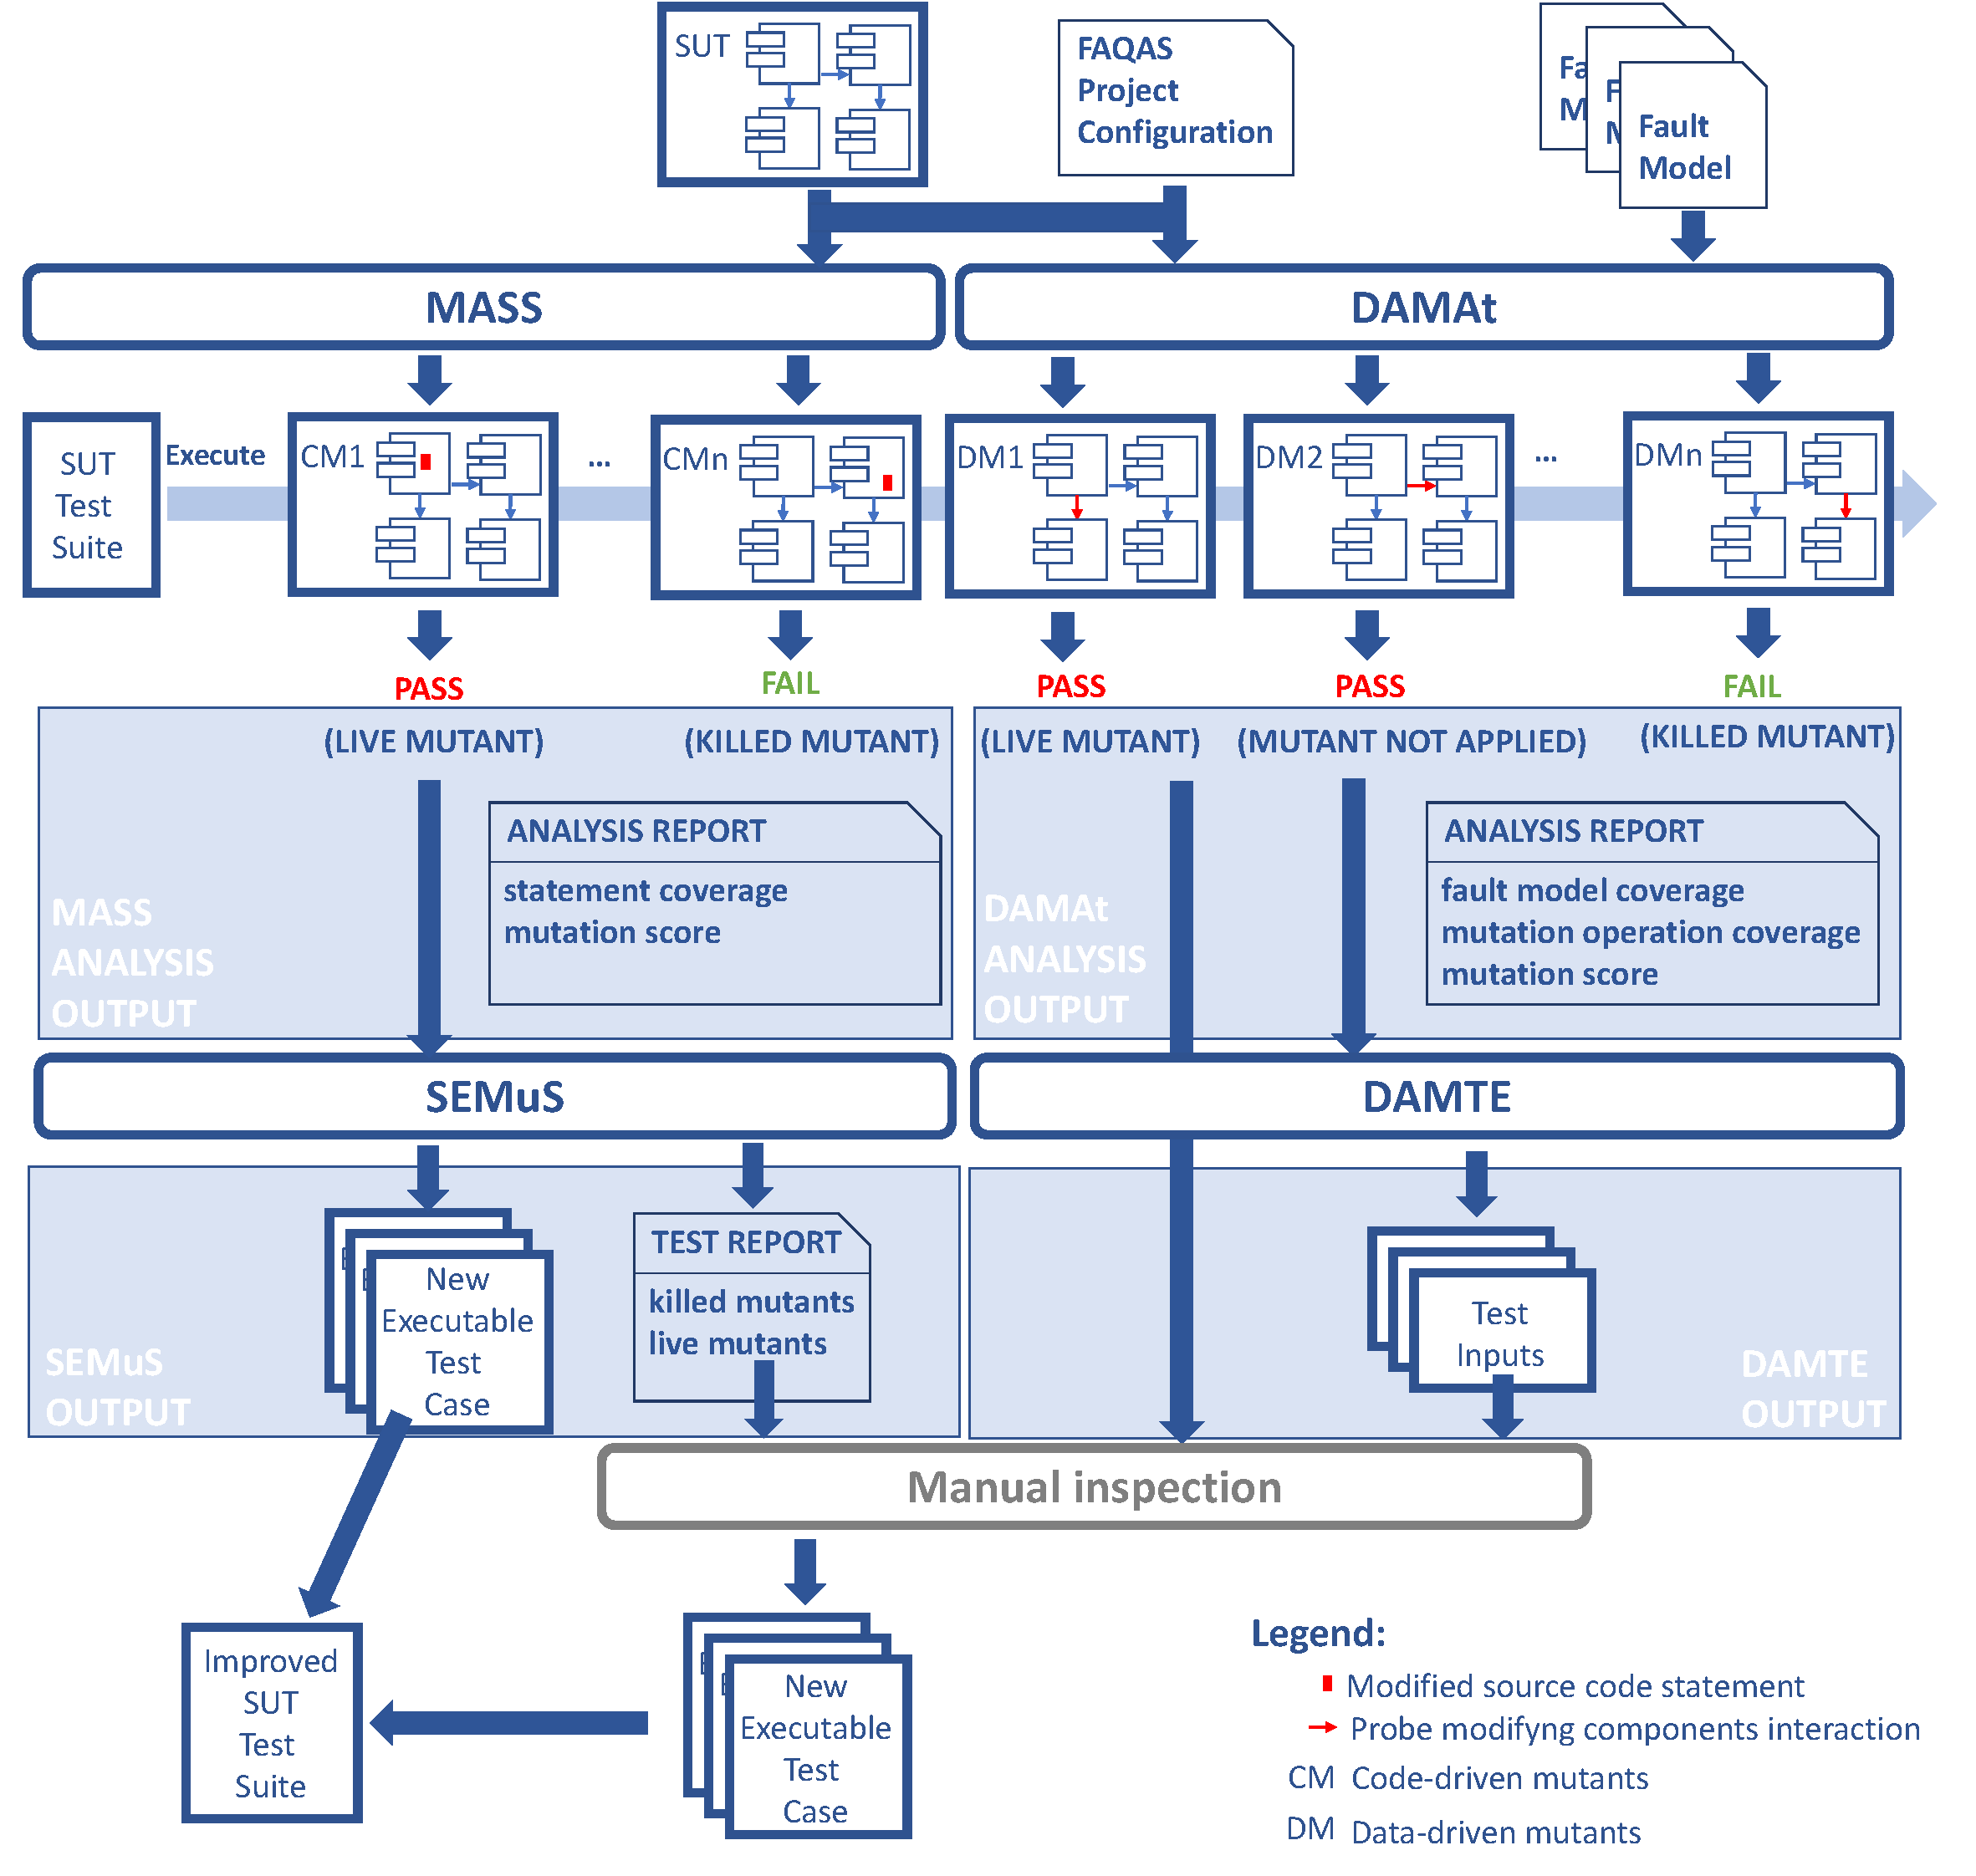
\includegraphics[width=0.7\textwidth]{images/FAQAS-overview.pdf}
\caption{Overview of the FAQAS toolset}
\label{fig:FAQAS:toolset}
\end{center}
\end{figure*}

Figure~\ref{fig:FAQAS:toolset} provides an overview of the input and outputs of the FAQAS toolset. It relies on the idea of generating multiple modified versions of the software system under test (SUT), some are derived by modifying the implementation of the software (code-driven mutants) other by integrating a mutation API that alters the messages exchanged by the software components of the SUT (data-driven mutants). 
The SUT test suite shall be executed with all the mutants, if it is effective then it shall fail with each of them. The mutants for which a failure is not observed are said to be \EMPH{live} and indicate a pitfall in the test suite.
All the FAQAS tools take as input the software under test (SUT), its test suite, and a set of configuration files. 

\EMPH{MASS} generates code-driven mutants. It integrates a pipeline of solutions that make mutation analysis feasible with large SUT. The three main contributions of MASS are (1) the automated identification of trivially equivalent mutants using an ensemble of compiler optimization options, (2) the computation of the mutation score based on mutant sampling with fixed size confidence interval approach (FSCI), (3) the automated identification of equivalent mutants based on coverage. 
MASS reports the set of live mutants, the set of killed mutants (i.e., mutants that are discovered by the test suite), and information useful to draft a verification report, which includes the statement coverage of the SUT test suite and the mutation score (i.e., the percentage of mutants discovered by the test suite).

\EMPH{DAMAt} generates mutants for data-driven mutation analysis. Data-driven mutation analysis is a research contribution of FAQAS. Instead of mutating the implementation of the SUT, it consists of altering the data exchanged by software components. 
DAMAt relies on fault models that specify how to mutate the data exchanged by software components through data-driven mutation operators. DAMAt can automatically alter data that is stored in data buffers (e.g., before serialization on the communication channel).
DAMAt enables the simulation of faults that affect simulated components (e.g., sensors), which is not feasible with traditional, code-driven mutation analysis. 
DAMAt generates as output a set of killed mutants (i.e., mutants that, during testing, successfully alter the data, and lead to test case failures), a set of live mutants (i.e., mutants that, during testing, successfully alter the data, but do not lead to test case failures), and a set of mutants not applied (i.e., mutants that, during testing, could not alter any data because the data they target is never exercised by the SUT); also, it provides information useful to draft a verification report, which includes the fault model coverage (i.e., percentage of fault models with at least one mutant applied), the mutation operation coverage (i.e., percentage of mutants applied), and the mutation score.

\EMPH{SEMuS} automatically generates executable unit test cases based on code-driven mutation analysis results. The generated unit test cases detect mutants not detected by the original test suite. The generated test cases include test oracles that shall be manually validated by engineers, which enables detecting faults. The generated test cases can be integrated into regression test suites.

SEMuS takes as input the list of live mutants detected by MASS. It generates a set of additional test cases that can be integrated into the SUT test suite. Also, it reports the list of killed mutants and the list of mutants that remain live (i.e., for which SEMuS did not generate a test case that kill them). Live mutants shall be manually inspected by engineers to either determine if they are equivalent or to manually derive a test case capable of killing them.

\EMPH{DAMTE} is a manual procedure supported by an automated symbolic execution toolset; it automatically identifies the test inputs that make software components exchange the data targeted by data-driven mutation operators. The derived test inputs can then be manually integrated into the SUT test suite.
 
The activity also included an extensive empirical evaluation demonstrating the feasibility, effectiveness, and scalability of the proposed toolsets in the space context, as described in the following sections.
 
%FAQAS.drawio.pdf

%Sections~\ref{ch:mass:approach} to~\ref{sec:data:test_suite_augmentation} provide an overview of the FAQAS tools: MASS, SEMuS, DAMAt, and DAMTE.
%Section~\ref{chapter:caseStudies} introduces the case study subjects considered for empirical evaluation.
%Section~\ref{sec:summary:results} provides an overview of the empirical results obtained.
%Section~\ref{sec:conclusion} concludes this report.



%% !TEX root = MAIN.tex

\section{Acronyms and Abbreviations}
\label{sec:acronyms}


%@{\extracolsep{\fill}}
\begin{tabular}{|p{1.5cm}|p{14.5cm}|}
%&\TODO{Add acronyms. OSCAR: I've add some...} \\

%ACO & Ant Colony Optimization\\
D1& Deliverable 1 of FAQAS activity, \emph{Analysis and Survey of Mutation Testing}\\
D2& Deliverable 2 of FAQAS activity, \emph{Study of Mutation Testing Applicability to Space Software}\\
FOM & First Order Mutant\\
HOM & Higher-Order Mutant\\
LOC & Lines of Code\\
%SBST & Search Based Software Testing\\
%Fabrizio: we cannot use SE as acronym
%SE & Symbolic Execution\\
SOM & Second Order Mutant\\
SUT & Software Under Test\\
TS & Test Suite\\
UL HPC & University of Luxembourg High Performance Computing

%Comment #2:
%When generating the pdf file, make sure to have the index of the document on the left, so that the document is easier to navigate.
%Author: Pedro Barrios Subject: Sticky Note Date: 28/02/2020, 09:18:06
%Comment #3:
%Try to make the document a bit more friendly to read (e.g. by adding some sentences in bold (see the highlighted ones for this paragraph), making bigger
%separation between paragraphs, ...)
%Author: Pedro Barrios Subject: Sticky Note Date: 28/02/2020, 09:18:11
%Comment #4:
%It is perhaps interesting to add a chapter with some basic definitions?
%e.g. equivalent mutant, redundant mutant, mutation score, killed mutant, live mutant, weak mutation, ...
%Author: Pedro Barrios Subject: Sticky Note Date: 28/02/2020, 09:18:18
%Comment #5:
%Please, consider to add more examples.

                                                           
\end{tabular}
\normalsize

\clearpage

% !TEX root =  Main.tex
\chapter{State-of-the-art}
\label{ch:stateOfTheArt}

%\item The literature on mutation analysis/testing mostly focuses on modifying the code of the software under test (hereafter, code-driven approaches). Some approaches rely on modifying models, but they aim to generate test cases not assessing test suites. There are no approaches that assess test suites by changing the data generated by software components (hereafter, data-driven approaches).
%\item The mutation operators widely adopted to perform code-driven mutation analysis are the sufficient set of operators and the set of deletion operators. Other operators did not receive the same degree of attention in the literature. For example, higher-order mutation operators are reported to be easier to kill than the first-order ones (i.e., they are less effective in assessing test suites limitations); consequently, they had been adopted less in empirical studies.                   
%o	The literature lacks mutation analysis approaches that enable simulating errors in the presence of simulated components (e.g., sensors). 
%o	Scalable approaches targeting mutation testing (i.e., automatically generating test cases that kill mutants) are few. The most promising ones rely on symbolic execution based on LLVM, which might be inapplicable for onboard flight software compiled for specific architectures. 

This chapter briefly discusses the applicability, in the context of space software, of existing solutions related to the four contributions of FAQAS: code-driven mutation analysis, 
code-driven mutation testing, data-driven mutation analysis, 
data-driven mutation testing.

\section{Code-driven mutation analysis}
\label{sec:background}

Mutation analysis can drive the generation of test cases, which is referred to as \INDEX{mutation testing} in the literature.
A detailed overview of mutation testing and analysis solutions and optimizations can be found in recent surveys~\cite{jia2010analysis,papadakis2019mutation}.

\subsection{Mutation Adequacy and Mutation Score computation}
\label{background:adequacy}
A mutant is said to be killed if at least one test case in the test suite fails when exercising the mutant.
Mutants that do not lead to the failure of any test case are said to be live.
Three conditions should hold for a test case to kill a mutant: \emph{reachability} (i.e, the test case should execute the mutated statement), \emph{necessity} (i.e., the test case should reach an incorrect intermediate state after executing the mutated statement), and \emph{sufficiency} (i.e., the final state of the mutated program should differ from that of the original program)~\cite{offutt1997automatically}.

The mutation score, i.e., the percentage of killed mutants, is a quantitative measure of the quality of a test suite. Recent studies have shown that achieving a high mutation score improves significantly the fault detection capability of a test suite
~\cite{papadakis2018mutation},  
\JMR{1.6}{
a result which contrasts with that of structural coverage measures~\cite{Chekam:17}. However, a very high mutation score (e.g., above 75\%) is required to achieve a higher fault detection rate than the one obtained with other coverage criteria, such as statement and branch coverage~\cite{Chekam:17}. In other words, there exists a strong association between a high mutation score and a high fault revelation capability for test suites.}
 

The capability of a test case to kill a mutant also depends on the observability of the program state. To overcome the limitations due to observability, different strategies to identify killed mutants can be adopted; they are known as strong, weak, firm, and flexible mutation coverage~\cite{ammann2016introduction}. 
\JMR{1.11 3.9}{With strong mutation, to kill a mutant, there shall be an observable difference between the outputs of the original and mutated programs.  
With weak mutation, the state (i.e., the valuations of the program variables in scope) of the mutant shall differ from the state of the original program, after the execution of the mutated statement~\cite{Lee1994}. 
With firm mutation, the state of the mutant shall differ from the state of the original program at execution points between the first execution of the mutated statement and the termination of the program~\cite{Woodward88}. 
Flexible mutation coverage consists of checking if the mutated code leads to object corruption~\cite{mateo2012validating}}.
For space software, we suggest to rely on strong mutation because it is the only criterion that truly assesses the fault detection capability of the test suite; indeed, it relies on a mutation score that reflects the percentage of mutants leading to test failures. With the other mutation coverage criteria, a mutant is killed if the state of the mutant after  execution of the mutated statement differs from the one observed with the original code, without any guarantee that either the erroneous values in state variables will propagate or the test oracles will detect them. 




\subsection{Mutation Operators}
\label{sec:related:operators}

%% !TEX root =  ../Main.tex

\newcommand{\op}{\mathit{op}}
\newcommand{\ArithmeticSet}{ \texttt{+}, \texttt{-}, \texttt{*}, \texttt{/}, \texttt{\%} }
\newcommand{\LogicalSet}{ \texttt{&&}, \texttt{||} }
\newcommand{\RelationalSet}{ \texttt{>}, \texttt{>=}, \texttt{<}, \texttt{<=}, \texttt{==}, \texttt{!=} }
\newcommand{\BitWiseSet}{ \texttt{\&}, \texttt{|}, \land }
\newcommand{\ShiftSet}{ \texttt{>>}, \texttt{<<} }


\begin{table}[h]
\caption{Implemented set of mutation operators.}
\label{table:operators} 
\centering
\scriptsize
\begin{tabular}{|@{}p{4mm}@{}|@{}p{2cm}@{\hspace{1pt}}|@{}p{11.1cm}@{}|}
\hline
&\textbf{Operator} & \textbf{Description$^{*}$} \\
\hline
\multirow{7}{*}{\rotatebox{90}{\emph{Sufficient Set}}}&ABS               & $\{(v, -v)\}$	\\
\cline{2-3}
&AOR               & $\{(\op_1, op_2) \,|\, \op_1, \op_2 \in \{ \ArithmeticSet \} \land \op_1 \neq \op_2 \} $       \\
&    			  & $\{(\op_1, \op_2) \,|\, \op_1, \op_2 \in \{\texttt{+=}, \texttt{-=}, \texttt{*=}, \texttt{/=}, \texttt{\%} \texttt{=}\} \land \op_1 \neq \op_2 \} $       \\
\cline{2-3}
&ICR               & $\{i, x) \,|\, x \in \{1, -1, 0, i + 1, i - 1, -i\}\}$           \\
\cline{2-3}
&LCR               & $\{(\op_1, \op_2) \,|\, \op_1, \op_2 \in \{ \texttt{\&\&}, || \} \land \op_1 \neq \op_2 \}$            \\
&				  & $\{(\op_1, \op_2) \,|\, \op_1, \op_2 \in \{ \texttt{\&=}, \texttt{|=}, \texttt{\&=}\} \land \op_1 \neq \op_2 \}$            \\
&				  & $\{(\op_1, \op_2) \,|\, \op_1, \op_2 \in \{ \texttt{\&}, \texttt{|}, \texttt{\&\&}\} \land \op_1 \neq \op_2 \}$            \\
\cline{2-3}
&ROR               & $\{(\op_1, \op_2) \,|\, \op_1, \op_2 \in \{ \RelationalSet \}\}$            \\
&				  & $\{ (e, !(e)) \,|\, e \in \{\texttt{if(e)}, \texttt{while(e)}\} \}$ \\
\cline{2-3}
&SDL               & $\{(s, \texttt{remove}(s))\}$            \\
\cline{2-3}
&UOI               & $\{ (v, \texttt{--}v), (v, v\texttt{--}), (v, \texttt{++}v), (v, v\texttt{++}) \}$            \\   
\hline
\hline
\multirow{5}{*}{\rotatebox{90}{\emph{OODL}}}&AOD               & $\{((t_1\,op\,t_2), t_1), ((t_1\,op\,t_2), t_2) \,|\, op \in \{ \ArithmeticSet \} $       \\ 
\cline{2-3}
&LOD               & $\{((t_1\,op\,t_2), t_1), ((t_1\,op\,t_2), t_2) \,|\, op \in \{  \} \}$       \\ 
\cline{2-3}
&ROD               & $\{((t_1\,op\,t_2), t_1), ((t_1\,op\,t_2), t_2) \,|\, op \in \{ \RelationalSet \} \}$       \\ 
\cline{2-3}
&BOD               & $\{((t_1\,op\,t_2), t_1), ((t_1\,op\,t_2), t_2) \,|\, op \in \{ \BitWiseSet \} \}$       \\ 
\cline{2-3}
&SOD               & $\{((t_1\,op\,t_2), t_1), ((t_1\,op\,t_2), t_2) \,|\, op \in \{ \ShiftSet \} \}$       \\ 
%\hline
%COR               & $\{(\op_1, \op_2) \,|\, \op_1, \op_2 \in \{ \texttt{\&\&}, \texttt{||}, \land \} \land \op_1 \neq \op_2 \}$            \\
\hline
\hline
\multirow{3}{*}{\rotatebox{90}{\emph{Other}}}&LVR			& $\{(l_1, l_2) \,|\, (l_1, l_2) \in \{(0,-1), (l_1,-l_1), (l_1, 0), (\mathit{true}, \mathit{false}), (\mathit{false}, \mathit{true})\}\}$\\
&&\\
&&\\
\hline
\end{tabular}

$^{*}$Each pair in parenthesis shows how a program element is modified by the mutation operator. Th eleft element of the pair is replaced with the right element. We follow standard syntax~\cite{kintis2018effective}. Program elements are literals ($l$), integer literals ($i$), boolean expressions ($e$), operators ($\op$), statements ($s$), variables ($v$), and terms ( $t_i$, which might be either variables or literals).
\end{table}


Mutation analysis introduces small syntactical changes into the code (source code or machine code) of a program through a set of mutation operators that simulate programming mistakes. 



The  \emph{sufficient set of operators} is widely used for conducting empirical evaluations ~\cite{offutt1996experimental,rothermel1996experimental,andrews2005mutation,kintis2017detecting}. 
The original sufficient set, defined by Offutt et al., is composed of the following operators: Absolute Value Insertion (ABS), Arithmetic Operator Replacement (AOR), Integer Constraint Replacement (ICR), Logical Connector Replacement (LCR), Relational Operator Replacement (ROR), and Unary Operator Insertion (UOI)~\cite{offutt1996experimental}.
Andrews et al.~\cite{andrews2005mutation} have also included the 
\emph{statement deletion operator} (SDL)~\cite{delamaro2014designing}, which ensures that every pointer-manipulation and field-assignment statement is tested. 

The sufficient set of operators enables an accurate estimation of the mutation score of a test suite~\cite{siami2008sufficient}; furthermore, the mutation score computed with the sufficient set is a good estimate of the fault detection rate (i.e., the portion of real faults discovered) of a test suite~\cite{andrews2005mutation,Just:RealFaults:2014}. 

However, empirical work has shown that, to maximize the detection of real faults, a set of operators should be used in addition to the sufficient set: Conditional Operator Replacement (COR),
Literal Value Replacement (LVR), and Arithmetic Operator Deletion (AOD)~\cite{Kintis2018}. 


\CHANGED{The SDL operator has inspired the definition of mutation operators (e.g., \emph{OODL operators}) that delete portions of program statements, with the objective of replacing the sufficient set with a simpler set of mutation operators.
The OODL mutation operators include the delete Arithmetic (AOD), Bitwise (BOD), Logical (LOD), Relational (ROD), and Shift (SOD) operators.}
\JMR{3.8}{Empirical results show that deletion operators produce significantly fewer equivalent mutants\footnote{\JMRCHANGE{For example, statement deletion can lead to equivalent mutants only if statements are redundant, which is unlikely~\cite{Offut:2013}.}}}
\cite{delamaro2014designing,delamaro2014experimental} and, furthermore, 
test suites that kill mutants generated with both SDL and OODL operators kill a very high percentage of all mutants (i.e., 97\%)~\cite{delamaro2014experimental}. 

Another alternative to the sufficient set of operators is the generation of \emph{higher order mutants}, which result from the application of multiple mutation operators for each mutation~\cite{jia2009higher,kintis2010evaluating,offutt1992investigations,papadakis2010empirical}. However, higher order mutants are \CHANGED{easier to  kill
than the first order ones (i.e., less effective to assess test suites limitations)}~\cite{papadakis2010mutation,papadakis2019mutation}, and there is 
\CHANGED{limited empirical evidence regarding which mutation operators should be combined to resemble real faults and minimize the number of redundant mutants~\cite{papadakis2019mutation}.}



\subsection{Compile-time Scalability}
\label{sec:compile:time}


\JMR{1.12}{The potentially large size of the software under test, combined with the large number of available mutation operators, may make the compilation of all  mutants infeasible.}

To reduce the number of invocations to the compiler to one, \emph{mutant schemata} include all the mutations into a single executable~\cite{untch1993mutation}. 
With mutant schemata, the mutations to be tested are selected at run-time through configuration parameters. This may lead to a compilation speed-up of 300\% \cite{papadakis2010automatic}. 


Another solution to address compile-time scalability issues consists of \emph{mutating machine code}  (e.g., binary code~\cite{becker2012xemu}, assembly language~\cite{crouzet2006sesame},
Java bytecode~\cite{ma2006mujava}, 
 and
.NET bytecode~\cite{derezinska2011object}), thus avoiding the execution of the compilation process after creating a mutant. 
A common solution consists of mutating the
 LLVM Intermediate Representation (IR) \cite{hariri2016evaluating}, 
which enables the development of mutants that work with multiple programming languages~\cite{hariri2019comparing} and facilitates the integration of optimizations based on dynamic program analysis~\cite{denisov2018mull}.


Unfortunately, the mutation of machine code 
may lead to mutants that are not representative of real faults \JMRCHANGE{(i.e., faults caused by human mistakes at development time)} because they are impossible to generate from the source code\JMR{3.10}{~\cite{denisov2018mull}.
For instance, a function invocation in the source code may lead to hundreds of machine code instructions (e.g., the function call \emph{std::vector::push\_back} leads to 200 LLVM IR instructions) and, consequently, some of the mutants derived from such instructions cannot be derived by mutating the source code.}
In the case of IR mutation, some of these impossible mutants can be automatically identified~\cite{denisov2018mull}; however,
the number of generated mutants tend to be higher at the IR level than at the source code level, which may reduce scalability~\cite{hariri2019comparing}.
 In addition, we have encountered three problems that prevented the application of 
 mutation analysis tools based on LLVM IR to our case study systems.
First, space software relies on compiler pipelines (e.g., RTEMS~\cite{RTEMS}) that include architecture-specific optimizations not supported by LLVM. 
Second, there is no guarantee that the executables generated by LLVM are equivalent to those produced by the original compiler.
 Third, efficient toolsets based on LLVM often perform mutations dynamically~\cite{denisov2018mull}, which is infeasible when the software under test needs to be executed within a dedicated simulator, a common situation with space software and many other types of embedded software in cyber-physical systems.




\subsection{Runtime Scalability}
\label{sec:scalability}

A straightforward mutation analysis process consists of executing the full test suite against every mutant; however, it may lead to scalability problems in the case of a large software under test (SUT) with expensive test executions.
\emph{Simple optimizations} that can be applied to space software consist of (S1) stopping the execution of the test suite when the mutant has been killed, (S2) executing only those test cases that cover the mutated statements~\cite{delamaro1996proteum}, and (S3) rely on timeouts to automatically detect infinite loops introduced by mutation~\cite{papadakis2019mutation}. 

\emph{Split-stream execution} consists of generating a modified version of the SUT that creates multiple processes (one for each mutant) only when the mutated code is reached \cite{king1991fortran,tokumoto2016muvm}, thus saving time and resources. Unfortunately, it cannot be applied in the case of space software that needs to run with simulators because, in general, the hosting simulator cannot be forked by the hosted SUT.

Another feasible solution consists of  \emph{randomly selecting a subset of the generated mutants}~\cite{zhang2010operator,gopinath2015hard,zhang2013operator}. 
Zhang et al. \cite{zhang2013operator} empirically demonstrated that a random selection of 5\% of the mutants is sufficient for 
estimating, with high confidence, the mutation score obtained with the complete mutants set.
Further,
they show that sampling mutants uniformly across different program elements (e.g., functions) 
leads to a more accurate mutation score prediction than sampling mutants globally in a random fashion. 
For large software systems that lead to thousands of mutants, random mutation analysis is the only viable solution. However, for very large systems such as the ones commonly found in industry, randomly selecting 5\% of the mutants may still be too expensive.

\CHANGEDOCT{Gopinath et al. estimate the number of mutants required for an accurate mutation score~\cite{gopinath2015hard}.
They rely on the intuition that, under the assumption of independence between mutants,
mutation analysis can be seen as a Bernoulli experiment in which the outcome of the test for a single mutant is a Bernoulli trial (i.e., mutant successfully killed or not) and, consequently, 
the mutation score should follow a binomial distribution.
They rely on Tchebysheff’s inequality~\cite{Tchebichef1867} to find a theoretical lower bound on the number of mutants required for an accurate mutation score. 
More precisely, they suggest that, with 1,000 mutants, 
the estimated mutation score differs from the real mutation score at most by 7 percentage points.
However, empirical results show that the binomial distribution provides a conservative estimate of the population variance and, consequently, 1,000 mutants enable in practice a more accurate estimate ($> 97\%$) of the mutation score than expected.}

In the statistics literature, the correlated binomial model~\cite{Bahadur}, 
and related models~\cite{Kupper1978,NG:ModifiedBinomialDistributions:1989,VanDerGeest:2005} are used when Bernoulli trials are not independent~\cite{Zhang:CrrelatedFirearm:NIST:2019}. 
In our work, based on the results achieved by Gopinath et al., we assume that the degree of correlation between mutants is limited and the binomial distribution can be used to accurately estimate the mutation score.
%which is supported by our empirical results (see Section~\ref{sec:evaluation}).
%  In Appendix B,
%  %~\ref{appendix:correlation}, 
%  we verify the correctness of our assumptions 
%%based on the analysis of the distribution of the mutation score in our empirical evaluation. 
%%In addition, our assumptions are demonstrated as being true by our empirical results (see Section~\ref{sec:evaluation}).}
%by reporting the degree of association between trials and by comparing the  probability mass function for the binomial and the correlated binomial distributions, for all our subjects.}



The statistics literature also provides a number of approaches for the computation of a sample size (i.e., the number of mutants, in our context) that enables estimates with a given degree of accuracy~\cite{Krejcie,Cochran,Bartlett,Krishnamoorthy07}. 
For binomial distributions, the most recent work is that of Gonçalves et al.~\cite{Goncalves2012}, that
determines the sample size by
relying on heuristics for the computation of confidence intervals for binomial proportions. 
A confidence interval has a probability $p_c$ (the confidence level) of including the estimated parameter (e.g., the mutation score). 
Results show that the largest number of samples required to compute a 95\% confidence interval is 1,568. 

If used to drive the selection of mutants, both the approaches of Gopinath et al. and Gonçalves et al., which suggest sampling at least 1,000 mutants, may be impractical when mutants are tested with large system test suites.


\CHANGED{An alternative to computing the sample size before performing an experiment is provided by sequential analysis approaches, which determine the sample size while conducting a statistical test~\cite{waldSequential}. 
Such approaches do not perform worst-case estimates and may thus lead to smaller sample sizes. For example, the sequential probability ratio test, which can be used to test hypotheses, has been used in mutation analysis as a condition to determine when to stop test case generation (i.e., when the mutation score is above a given threshold)~\cite{Hsu:90}. In our context, we are interested in point estimation, not hypothesis testing; in this case, 
the sample size can be determined through a fixed-width sequential confidence interval (FSCI), i.e., by computing the confidence interval after every new sample and then stop sampling when the interval is within a desired bound~\cite{Frey:FixedWidthSequentialConfidenceIntervals:AmericanStatistician:2010,Chen2013,Yaacoub:OptimalStopping}. 
Concerning the method used to compute the confidence interval in FSCI, the statistics literature~\cite{Frey:FixedWidthSequentialConfidenceIntervals:AmericanStatistician:2010} reports that the Wald method~\cite{WaldMethodVollset} minimizes the sample size but requires an accurate variance estimate. We will therefore resort to a non-parametric alternative, which is Clopper-Pearson~\cite{ClopperPearson}.
Note that FSCI 
has never been applied to determine the number of mutants to consider in mutation analysis.}

Other solutions to address \emph{runtime scalability problems} in mutation analysis  aim to \emph{prioritize test cases} to maximize the likelihood of executing first those that kill the mutants~\cite{just2012using,papadakis2011automatically,zhang2013faster}. The main goal is to save time by preventing the execution of a large subset of the test suite, for each mutant.
Previous work aimed at prioritizing faster test cases~\cite{just2012using} but this 
 may not be adequate with system-level test suites whose test cases have similar, long execution times.
Approaches that rely on data-flow analysis to identify and prioritize the test cases that likely satisfy the killing conditions~\cite{papadakis2011automatically} are prohibitively expensive and are unlikely to scale to large systems.
Other work~\cite{zhang2013faster} combines three coverage criteria:
(1) the number of times the mutated statement is exercised by the test case,
 (2) the proximity of the mutated statement to the end of the test case 
 (closer ones have higher chances of satisfying the sufficiency condition)
 , and (3) 
 the percentage of mutants belonging to the same class file of the mutated statement that were already killed by the test case. 
Criterion (3) is also used to reduce the test suite size, by only selecting the test cases above a given percentage threshold. 
Unfortunately, only criterion (1) seems applicable in our context; indeed, criterion (2) is ineffective with system test cases whose results are checked after long executions, while criterion (3) may be inaccurate when only a random, small subset of mutants is executed, as discussed above. 






%For \INDEX{test case reduction}, the idea is to remove those test cases that are somehow redundant (e.g., test cases that when removed from the test suites do not change the mutation score).
%Usaola et al. \cite{usaola2012reduction} proposed a greedy algorithm that iteratively selects  the test cases that kill most of the mutants that were not killed by the previously selected test cases. 
%%\DONE{No change to do here. However please keep them in mind for the current work.}
%Shi et al. \cite{shi2014balancing} assessed the effects of reducing the size of test suites with an experiment on 18 projects with a total of 261\,235 test cases. Their results show that \emph{it is possible to maintain constant the mutation score and reduce test suite size without loss in the \emph{fault detection rate}}. 
%On the same line, Zhang et al. \cite{zhang2013faster} suggest to define a subset of tests of the original test suite and to run the mutants against the subset, their assumption is that if the mutants cannot be killed by the subset also the original test suite will not be able to kill the mutants.
%
%
%




\subsection{Detection of Equivalent Mutants}
\label{sec:background:equivalent}

\JMR{1.13}{A mutant is equivalent to the original program when they both generate the same outputs for the same inputs.}
Although identifying equivalent mutants is an undecidable problem~\cite{madeyski2013overcoming,Bugg:Correctness:82}, several heuristics have been developed to address it. 

The simplest solution consists of relying on \emph{trivial compiler optimisations}~\cite{papadakis2015trivial, kintis2017detecting,papadakis2019mutation}, i.e., compile both the mutants and the original program with compiler optimisations enabled and then determine whether their executables match. In C programs, compiler optimisations can reduce the total number of mutants by 28\%~\cite{kintis2017detecting}.



Solutions that identify equivalent mutants based on \emph{static program analysis} (e.g., concolic execution~\cite{holling2016nequivack,Chekam2021} and bounded model checking~\cite{riener2011test}) 
show promising results \JMR{2.3}{(e.g., to automatically identify non-equivalent mutants for batch programs~\cite{Chekam2021})} but
they rely on static analysis solutions that cannot work with system-level test cases that execute with hardware and environment simulators in the loop.
Indeed, (1) simulation results cannot be predicted by pure static analysis,  (2) concolic execution tools, which rely on LLVM, cannot be run if the SUT executable should be generated with a specific compiler (see Section~\ref{sec:compile:time}),
\JMR{2.3}{ (3) there are no solutions supporting the concolic execution of large software systems within simulation environments
(state-of-the-art techniques work with small embedded software~\cite{Herdt2019}), and (4) communication among components not based on direct method invocations (e.g., through network or databases) is not supported by existing toolsets.}

Alternative solutions rely on \emph{dynamic analysis} and compare data collected when testing the original software and the mutants~\cite{grun2009impact,schuler2010covering,schuler2013covering,schuler2009efficient}.
The most extensive empirical study on the topic shows that nonequivalent mutants can be detected by counting the number of methods (excluding the mutated method) that, for at least one test case, either (1) have statements that are executed at a different frequency with the mutant, (2) generate at least one different return value, or (3) are invoked at a different frequency~\cite{schuler2013covering}. To determine if a mutant is non-equivalent, it is possible to define a threshold indicating the smallest number of methods with such characteristics. A threshold of one identifies non-equivalent mutants with an average precision above 70\% and an average recall above 60\%. This solution outperforms more sophisticated methods relying on dynamic invariants~\cite{schuler2009efficient}. Also, coverage frequency alone leads to results close to the ones achieved by including all three criteria above~\cite{schuler2013covering}. 
However, such approaches require some tailoring 
because collecting all required data 
(i.e., coverage frequency for every program statement, return values of every method, frequency of invocation of every method) has a computational and memory cost that may break real-time constraints.

\subsection{Detection of Redundant Mutants}
\label{sec:background:redundant}
Redundant mutants are either \emph{duplicates}, i.e., mutants that are equivalent with each other but not equivalent to the original program, or \emph{subsumed}, i.e., mutants that are not equivalent with each other but are killed by the same test cases. 

Duplicate mutants can be detected by relying on the same approaches adopted for equivalent mutants. 

According to Shin et al., subsumed mutants should not be discarded but analyzed to augment the test suite with additional test cases that fail with one mutant only~\cite{Shin:TSE:DCriterion:2018}. 
The augmented test suite has a higher
 fault detection rate than a test suite that simply satisfies mutation coverage; however, with large software systems the approach becomes infeasible because of the lack of scalable test input generation approaches.

% !TEX root = MAIN.tex

\subsection{Benchmark of State-of-the-art, Code-driven Mutation Testing Toolsets}
\label{sec:toolsComparison}

This section summarizes the outcome of an experiment performed to evaluate the applicability of state-of-the-art mutation testing tools in the space context, based on the case study systems of the project. 

To carry out this preliminary evaluation of mutation testing tools, we selected a set of tools presented in the literature based on the following criteria:

\begin{itemize}
	\item \textbf{Availability of source code.} To enable optimizations, the tool under analysis should be provided along with source code.
	\item \textbf{Applicability to C/C++ code.} The tool under analysis should be able to process C and C++ code.
	\item \textbf{Licence compatible with ESA Software Community Licence Permissive (ESA SCLP).} The licence of the tool under analysis, should enable redistributing the tool itself within the FAQAS framework, which is released under ESA SCLP.
	\item \textbf{Age.} To avoid problems due to support for recent libraries, we should prioritize tools that are recent and actively developed.
\end{itemize}


The first three criteria mentioned above constitute mandatory requirements. 
Tools not meeting these requirements are not selected for evaluation in our context because they cannot be integrated into the FAQAS framework.

% !TEX root =  ../MAIN.tex


\setlength\LTleft{0pt}
\setlength\LTright{0pt}
\scriptsize 
\begin{longtable}{@{\extracolsep{\fill}}|p{3.4cm}|p{2.7cm}|p{7cm}|@{}}
\caption{\normalsize Summary of Data-Driven Mutation Testing Benchmarks.}
\label{table:mutationtools} \\
\hline
\textbf{Reference}                   & \textbf{Approach/Tool Name}      & \textbf{Evaluation} \\
\hline
Hariri \& Shi 2018          & SRCIRor                 &
\begin{minipage}[t]{6.5cm}
\textbf{Source code availability.} Yes, https://github.com/TestingResearchIllinois/srciror.\\
\textbf{Applicability to C/C++ code.} Yes.\\
\textbf{ESA SCLP Compatible.} Yes, released under NCSA, https://opensource.org/licenses/NCSA, which allows redistribution and relicensing.\\
\textbf{Age.} Aged, last update in September 2018.\\
\textbf{Outcome. The tool is applicable in space context.} 
\end{minipage}\\
\hline
Wang et al. 2017            & Accmut                  &
\begin{minipage}[t]{6.5cm}
\textbf{Source code availability.} Yes, https://github.com/wangbo15/accmut/\\
\textbf{Applicability to C/C++ code.} Yes.\\
\textbf{ESA SCLP Compatible.} Yes, released under NCSA, https://opensource.org/licenses/NCSA, which allows redistribution and relicensing.\\
\textbf{Age.} Aged, last update in January 2018.\\
\textbf{Outcome. Depends on CLANG/LLVM, which prevents compilations for some sysems.} 
\end{minipage}\\
\hline
Phan et al. 2018            & MUSIC                   &
\begin{minipage}[t]{6.5cm}
\textbf{Source code availability.} Yes, https://github.com/swtv-kaist/MUSIC/\\
\textbf{Applicability to C/C++ code.} Yes.\\
\textbf{ESA SCLP Compatible.} No. The software is licensed with proprietary licence. In private communication via e-mail, authors have shown to be available to relicensing, however this might not fit the budget of the project.\\
\textbf{Age.} Recent, last update in July 2019.\\
\end{minipage}\\
\hline
Denisov \& Pankevich 2018   & Mull                    &
\begin{minipage}[t]{6.5cm}
\textbf{Source code availability.} Yes, https://github.com/mull-project/Mull\\
\textbf{Applicability to C/C++ code.} Yes.\\
\textbf{ESA SCLP Compatible.} Yes. Apache Licence 2.0, https://opensource.org/licenses/Apache-2.0.\\
\textbf{Age.} Ongoing, last update in June 2020.\\
\textbf{Outcome. The tool requires compilation with CLANG/LLVM, which leads to compilation errors with systems depending on RTEMS. Also, natively, Mull performs mutations on the fly through just-in-time compilation features, which is inapplicable if the SUT is executed within a simulator.} 
\end{minipage}\\
\hline
Delgado et al. 2018         & MuCPP                   &
\begin{minipage}[t]{6.5cm}
\textbf{Source code availability.} No, only executables are available https://ucase.uca.es/mucpp/\\
\end{minipage}\\
\hline
Jia \& Harman 2008          & Milu                    &
\begin{minipage}[t]{6.5cm}
\textbf{Source code availability.} Yes, https://github.com/yuejia/Milu/\\
\textbf{Applicability to C/C++ code.} Yes.\\
\textbf{ESA SCLP Compatible.} Yes, released under NCSA licence, https://opensource.org/licenses/NCSA.\\
\textbf{Age.} Aged, last update in April 2018.\\
\textbf{Outcome. The tool generates a preprocessed source code that does not compile.} 
\end{minipage}\\
\hline
Brannstrom et al. 2015      & Dextool                 &
\begin{minipage}[t]{6.5cm}
\textbf{Source code availability.} Yes, https://github.com/joakim- brannstrom/dextool\\
\textbf{Applicability to C/C++ code.} Yes.\\
\textbf{ESA SCLP Compatible.} Yes, released under Mozilla public Licence 2.0, https://opensource.org/licenses/MPL-2.0.\\
\textbf{Age.} Ongoing, last update in June 2020.\\
\textbf{Outcome. Depends on CLANG/LLVM, which prevents compilations for some sysems.} 
\end{minipage}\\
\hline
Delamaro et al. 2001        & Proteum                 &
\begin{minipage}[t]{6.5cm}
\textbf{Source code availability.} Yes, https://github.com/magsilva/proteum.\\
\textbf{Applicability to C/C++ code.} Yes.\\
\textbf{Age.} Aged, last update December 2015.\\
\end{minipage}\\
\hline
Shariar and Zulkernine 2008 & Function Calls Mutation &
\begin{minipage}[t]{6.5cm}
\textbf{Source code availability.} No.\\
\end{minipage}\\
\hline
Dans \& Hierons 2001        & Floating-point Mutation &
\begin{minipage}[t]{6.5cm}
\textbf{Source code availability.} No.\\
\end{minipage}\\  

\hline                                                           
\end{longtable}


\normalsize

Table~\ref{table:mutationtools} provides the list of selected tools along with the evaluation results. We do not evaluate all the criteria when one of the mandatory requirements is not met.
For what it concerns the compatibility with the ESA Software Community Licence Permissive, we consider the licenses NCSA and Apache Licence 2.0 compatible. 
Indeed, both the two licences allow for redistribution of the software, a condition that is sufficient to release a mutation testing tool as component of the FAQAS framework.

For our evaluation we then selected the five most recent tools that fulfill our mandatory requirements: SRCIRor, Mull, Dextool, Accmut, and Milu. Proteum has been discarded because its latest stable version dates back to December 2015; on May 2020 a few changes had been made on Proteum GitHub repository, however, the up to date version is indicated by its developer as not usable.

To evaluate the applicability of existing mutation testing tools to space software, we evaluated each mutation testing tool considered in our study against the same case study system of the project, i.e., the System Test Suite for ESAIL provided by LXS. We selected this case study system, because (1) it is the largest case study system of FAQAS in terms of lines of code, (2) the ESAIL system test suite requires that the full software is compiled and all the required libraries linked (this may complicate the use of tools that cannot parse all the source code), (3) the software under test (SUT) is executed within a system emulator (SVF) that requires the SUT to respect its real-time constraints. ESAIL consists of 924 source files (719 files with extension ``.c'' and 205 with extension ``.h''). In total, it consists of 74,161 LOC. ESAIL is compiled with sparc-rtems4.8-gcc, a tailored version of the gcc compiler for sparc systems, the compiler is provided by Cobham Gaisler\footnote{https://www.gaisler.com/index.php/products/operating-systems/rtems}.

To draw a final outcome for or evaluation (see Table~\ref{table:mutationtools}), we applied each selected tool to ESAIL and verified if the mutation testing tool could successfully create mutated version of ESAIL that can be compiled and executed within the SVF.
Out of all the selected tools, only SRCIRor had been successfully applied to ESAIL.




\subsection{Summary}
\label{sec:back:summary}

We aim to rely on the sufficient set of operators since it has been successfully used to generate a mutation score that accurately estimates the fault detection rate for software written in C and C++, languages commonly used in embedded software.
%Based on recent results, we should however extend the sufficient set with LVR, and all the operators belonging to OODL.
\CHANGED{Further, since recent results have reported on the usefulness of both LVR and OODL operators to support the generation of test suites with high fault revealing power~\cite{Kintis2018}, the sufficient set may be extended to include these two operators as well.}

To speed up mutation analysis by reducing the number of mutants, we should consider the SDL operator alone \CHANGED{or in combination with the OODL operators}. However, such heuristic should be carefully evaluated to determine the level of confidence we can expect.

Among compile time optimizations, only mutant schemata appear to be feasible with space software.
Concerning scalability, simple optimizations (i.e., S1, S2, and S3 in Section~\ref{sec:scalability}) are feasible. Alternative solutions are the ones relying on mutant sampling and coverage metrics. 
However, to be applied in a safety or mission critical context, mutant sampling approaches should provide guarantees about the 
level of confidence one may expect. Currently, this can only be achieved with approaches requiring a large number of sampled mutants (e.g., $1,000$).  Therefore, sequential analysis based on FSCI, which minimizes the number of samples and provides accuracy guarantees, appears to be the most appropriate solution in our context.
Further, test suite selection and prioritization strategies based on code coverage require some tailoring to cope with real time constraints.
% when mutant sampling rates are below 5\% should be evaluated. 
%Furthermore, code coverage metrics that are feasible for space software need to be defined.

Equivalent mutants can be identified through trivial compiler optimizations and the analysis of coverage differences; however, it is necessary to define and evaluate appropriate coverage metrics. The same approach can be adopted to identify duplicate mutants. The generation of test cases that distinguish subsumed mutants is out of the scope of this work.

\JMR{1.1 3.3}{A high-level description of a possible mutation testing pipeline was proposed in a recent survey\footnote{The main objective of such pipeline was to walk the reader through the survey, not to propose a precise and feasible solution.}~\cite{papadakis2019mutation}. It consists of the following sequence of activities: select (sample) mutants, compile mutants, remove equivalent and redundant mutants, generate test inputs that kill mutants, execute mutants, compute mutation score, reduce test suites and prioritize test cases. 
Unfortunately, such pipeline does not enable the integration of many optimizations proposed above, which further motivates our work. For example, it cannot support FSCI-based sampling, which requires mutants sampling to be coupled with mutants execution. Also, it does not envision the detection of equivalent and redundant mutants based on code coverage. Moreover, it only partially addresses scalability issues since test suite reduction and prioritization are performed after mutation analysis. 
Further, it includes a test input generation step that is not feasible in the context of CPS.
Finally, it has never been implemented and therefore its feasibility has not been evaluated.}




% !TEX root = ../MAIN.tex

\section{Data-driven Mutation Analysis}
\label{sec:background}

\INDEX{Data-driven mutation analysis} evaluates the effectiveness of a test suite in detecting \INDEX{interoperability faults}. The CPS literature reports on four different interoperability types~\cite{Givehchi:2017}: technical (which concerns communication protocols and  infrastructure), syntactic (which concerns data format), semantic (which concerns the exchanged information, that is, errors in the processing of exchanged data), and cross-domain interoperability (which concerns interaction through business process languages such as BPEL~\cite{BPEL}).
\REVTOOL{P-1}{For example, a technical interoperability problem may concern two components working with two different network protocols (e.g., TCP VS UDP), a syntactic interoperability problem is that of two components using different keywords to specify a field in a json~\cite{JSON} data file (e.g., "temperature" and "temp"), a semantic interoperability problem is that of a control software that does not take appropriate actions when the voltage of the board is above nominal range, cross domain interoperability is that of a web service not following the expected flow of remote calls.}
Technical and syntactic interoperability are provided by off-the-shelf hardware and libraries
(not tested by CPS developers) 
 while cross-domain interoperability concerns systems integrated in online services (e.g., energy plants) but is out of scope for the type of CPSs we target in this work, which are safety-critical CPSs like flight systems, robots, and automotive systems. In this paper, we thus focus on \INDEX{semantic interoperability} faults,
 that is, faults that affect CPS components integration and are triggered (i.e., lead to failures) in the presence of specific subsets of the data that might be exchanged by CPS components. We thus aim to ensure that a test suite fails when the data exchanged by CPS components is not the one specified by test cases (e.g., through simulator configurations).
%verifies that all the data exchanged by CPS components are correctly processed, that is, it  
Related work includes mutation analysis~\cite{jia2010analysis,papadakis2019mutation} and \INDEX{fault injection}~\cite{natella2016assessing} techniques.

\subsection{Mutation Analysis}


\textbf{Mutation analysis} concerns the automated generation of faulty software versions (i.e., mutants) through automated procedures called mutation operators~\cite{jia2010analysis,papadakis2019mutation}. The effectiveness of a test suite is measured by computing the mutation score, which is the percentage of mutants leading to failures when exercised by the test suite.

\INDEX{Mutation operators} introduce syntactical changes into the code of the \UPDATED{SUT}. The  \INDEX{sufficient set of operators} is implemented by most mutation analysis toolsets~\cite{offutt1996experimental,rothermel1996experimental,andrews2005mutation,kintis2017detecting,offutt1996experimental}. 
Unfortunately, these operators simulate faults concerning the implementation of algorithms (e.g., a wrong logical connector), which is usually tested in unit test suites that, by definition, do not exercise the communication among components, our target in this paper. 
Also, as stated in the Introduction, such operators can't be used to generate faulty data with simulated or off-the-shelf components.
\INDEX{Higher-order} mutation analysis~\cite{harman2010manifesto}, which simply combines multiple operators, has the same limitations.

\UPDATED{\INDEX{Components integration} is targeted by interface~\cite{delamaro2001interface}, integration~\cite{Grechanik:16}, contract-based~\cite{Jiang:ICSM:05}, and system-level mutation analysis~\cite{mateo2010mutation}. The former three assess the quality of integration test suites by introducing changes that concern function invocations 
(e.g., switch function arguments) and inter-procedural data-flow (e.g., alter assignments to variables returned to other components);
they can simulate integration faults in units integrated with API invocations but 
not interoperability problems concerning larger components communicating through channels (e.g., network).
\INDEX{System-level mutation} relies on operators for GUI components, which are out of our scope, and  configuration files, by applying simple mutations, such as deleting a line of text, and are unlikely to lead to interoperability problems.}



\subsection{Fault injection}

\INDEX{Fault injection techniques} simulate the effect of faults by altering, at runtime, the data processed by the \UPDATED{SUT}~\cite{natella2016assessing}. Faults are introduced according to a fault model that describes the type of fault to inject, the timing of the injection, and the part of the system targeted by the injection. Different from data-driven mutation analysis, fault injection techniques aim to stress the robustness of the software,  
%(e.g., determine if out-of-range input values can crash the system) 
not assess the quality of its test suites.
%(e.g., determine if in-range input values lead to test failures).



Faults affecting components' communication, 
CPU, or memory can simulated by performing bit flips 
%setting bits to zero and one, 
%or toggling bits~
\cite{tsai1999stress,barton1990fault,han1995doctor,dawson1996testing}.
\INDEX{Communication faults} are simulated also by duplicating or deleting packets, altering their sequence, or introducing incorrect identifiers, checksums, or counters~\cite{di2015evolutionary,di2015generating}.
Faults affecting \INDEX{signals} can be simulated by shifting the signal or increasing the number of signal segments~\cite{Matinnejad19}.
The largest set of faults affecting data exchanged through files or byte streams is simulated by Peach~\cite{PeachFuzzer}, which includes also protocol-specific fault injection procedures such as replacing host names with randomly generated ones.
In general, although existing techniques may simulate a large set of faults they do not cover all the CPS interoperability faults (see Section~\ref{sec:faultModelStructure}).

Approaches performing fault injections other than bit flips require a model of the data to modify.
The modelling formalisms adopted for this purpose are grammars~\cite{ghosh1998testing,Godefroid:GrammarBasedFuzzying:2008,godefroid2012sage,bounimova2013billions}, UML class diagrams~\cite{di2015evolutionary,di2015generating}, or block models~\cite{pham2016model,PeachFuzzer}.
Grammars are used to model textual data (e.g., XML), which is seldom exchanged by CPS components because of parsing cost. 
Block models enable specifying the representation to be used for consecutive blocks of bytes, which makes them applicable to a large set of systems; however, existing block model formalisms rely on the XML format, which is expensive to process and thus not usable with real-time systems~\cite{pham2016model,PeachFuzzer}.
The \INDEX{UML class diagram} is a formalism that
enables the specification of complex data structures and 
%support the generation of data faults that break complex 
data dependencies 
%(e.g., using the OCL language~\cite{OCL})
\cite{di2015evolutionary,di2015generating}; however, it requires loading the data as UML class diagram instances, which is too expensive for real-time systems. 

\subsection{Summary}

To summarize, the modification of the data exchanged by software components enables the simulation of communication and, therefore, semantic interoperability faults.
Test suites can thus be assessed by relying on fault injection techniques to mutate data. 
However, existing fault injection techniques do not target mutation analysis; consequently, we lack methods for the specification of fault models and metrics for the assessment of test suites. 
Also, a larger set of procedures for the modification of data is needed.
Finally, block models can effectively capture the structure of the data to modify but formalisms not relying on XML are needed. Our paper addresses such limitations.

%\textbf{Mutation testing implements grammar-based testing}
%
%\cite{Offutt2006} The paper discuss the idea that mutation analysis is a way to modify any software artifact such as program specifications, XML and input languages, based on its syntactic description (i.e., a grammar). More abstractly, mutation analysis can be referred to grammar-based testing, and this concept can be used to develop additional applications such as the mutation of finite state machines and use case collaboration diagrams.
%For example, programming languages are described in grammar notation, program behavior is described in finite state machines, and allowable inputs to programs are defined by grammars. With grammar-based testing, tests are created from the grammar.
%
%Instead, grammar-based input testing is based on grammars that formally define the syntax of the inputs to a program, method or software component. For example, a language's grammar defines the inputs of its compiler, and the XML schema defines the inputs of a XML parser. 
%Invalid inputs can be created by mutating input grammars. When mutating grammars, the mutants are the tests and we create valid and invalid strings. There is no ground string, so the notion of killing mutants does not apply to mutating grammars.
%In the paper, four grammar operators are defined (nonterminal replacement, terminal replacement, terminal and nonterminal deletion, and terminal and nonterminal duplication). 
%
%
%\subsection{Data Modeling}
%\label{sec:dataModeling}
%
%Approaches performing data mutation often require a data model to drive mutations (e.g., to decide how to alter a specific chunk of data). 
%However, some of the approaches do not require a data model. 
%These approaches are the ones that perform low level changes (e.g., bit flips) or that combine multiple low level changes driven by the data collected at runtime (e.g., code coverage information~\cite{gutmann2016fuzzing}).
%The main drawback of approaches that do not require a data model is that they can hardly be used in a mutation testing context.
%Indeed, without additional information (e.g., a data model) it is not possible to determine what should be the expected effect of modifying a randomly selected portion of an input, in turn, it is not possible to determine if the mutated data should lead to a test failure, trigger a robustness feature of the SUT, or simply go unnoticed because it does not alter the behaviour of the software (e.g., because it alters bytes that are copied as is by a data processing system).
%
%Three are the main solutions adopted for data modeling, the use of grammars~\cite{ghosh1998testing,Godefroid:GrammarBasedFuzzying:2008,godefroid2012sage,bounimova2013billions}, the use of UML models~\cite{di2015evolutionary}, and the use of block models~\cite{pham2016model,PeachFuzzer}.
%
%\subsubsection{Data modeling with grammars}
%
%Grammar-based approaches rely on a context-free grammar to specify the format of the data to be mutated. 
%Listing~\ref{JSONgrammar} shows an example of a grammar for the JSON format in BNF notation. Listing~\ref{JSONgrammarEBNF} shows the same grammar in EBNF notation. Listing~\ref{JSONfile} shows an example JSON file.
%
%Grammars are used by fuzzing approaches that alter input files to perform robustness testing~\cite{ghosh1998testing} and security testing~\cite{Appelt:SQLI:ISSTA:2014,Jan:ISSTA:2016}. They might be used to perform black-box mutations~\cite{ghosh1998testing} or white-box mutations that leverage code analysis to augment the coverage of the SUT~\cite{Godefroid:GrammarBasedFuzzying:2008}.
%% because of the large space of invalid inputs
%The main limitation of grammars is that they cannot be used to encode integrity constraints such as size-of, offset-of, length-of, and checksums~\cite{pham2016model}. 
%%JSONgrammar
%
%% !TEX root = ../MutationTestingSurvey.tex
\begin{minipage}{10cm}
\footnotesize
\begin{lstlisting}[caption=JSON grammar provided in~\cite{GramTest}., label=JSONgrammar]
<JSON>      ::= <object> | <array>
<array>     ::= "[" <value> {"," <value>} "]"
<object>    ::= "{" <property> {"," <property>} "}"
<property>  ::= <string> ":" <value>
<value>     ::= <object> | <array> | <boolean> | <string> | <number>
<boolean>   ::= true | false
<string>    ::= """ <alphas> """
<alphas>    ::= <alpha> [<alphas>]
<number>    ::= <digit> [<number>]
<alpha>	    ::= a | b | c | d | e | f | g | h | i | j | k | l | m | n | o | 
		p | q | r | s | t | u | v | w | x | y | z | A | B | C | D | 
		E | F | G | H | I | J | K | L | M | N | O | P | Q | R | 
		S | T | U | V | W | X | Y | Z
<digit>     ::= 0 | 1 | 2 | 3 | 4 | 5 | 6 | 7 | 8 | 9
\end{lstlisting}
\end{minipage}

%
%\subsubsection{Data modeling with UML models}
%
%Approaches relying on UML models~\cite{di2015generating,di2015evolutionary} use (i) class diagrams to capture the structure of inputs and outputs, (ii) expressions written with the Object Constraint Language (OCL)~\cite{OCL} to define relationships between the inputs and outputs, and (iii) UML stereotypes to capture a fault model driving the generation of test cases.
%Figure~\ref{fig:dataModel} shows a simplified data model taken from~\cite{di2015evolutionary} that captures the structure of the data transmitted by the Sentinel-1 ESA satellites~\cite{esaSentinel}.
%The model captures the structure of a network transmission; UML classes represent elements that contain multiple fields, while UML attributes model elements that cannot be further decomposed. For example, it shows that each transmission consists of a sequence of \emph{Virtual Channel Data Units (VCDUs)}. Each \emph{VCDU} begins with a \emph{Header}, followed by a \emph{PacketZoneHeader} and a \emph{PacketZone} that may contain a sequence of \emph{Packets} (if the packet zone is active).
%The \emph{VCDUs} in a transmission may belong to different virtual channels.
%Associations are used to represent containment relationships. In Figure~\ref{fig:dataModel}, the classes that model the VCDU and its Header are connected by an association.
%The attributes of a class represent the transmitted binary information. For example, attribute \emph{sequenceCount} of class \emph{Packet} is used to store information about the packet order.
%Figures~\ref{fig:transmissionData} to~\ref{fig:packet}, graphically presents Sentinel-1 transmission data as sequences of bytes.
%Stereotypes are used to capture the fault model of the system and their role is presented in Section~\ref{sec:data_operators}.
%
%\begin{figure}[t!]
%  \centering
%    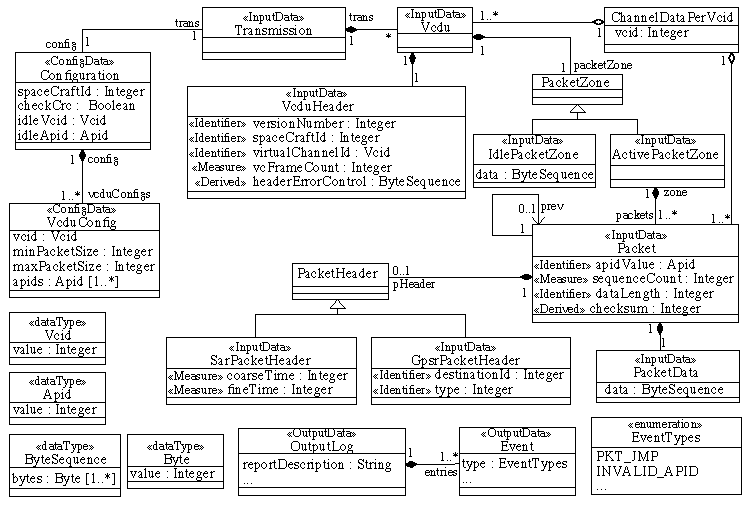
\includegraphics{images/classDiagramSmall}
%      \caption{Simplified input data model taken from~\cite{di2015evolutionary}.}
%      \label{fig:dataModel}
%\end{figure}
%
%\begin{figure}[h]
%  \centering
%    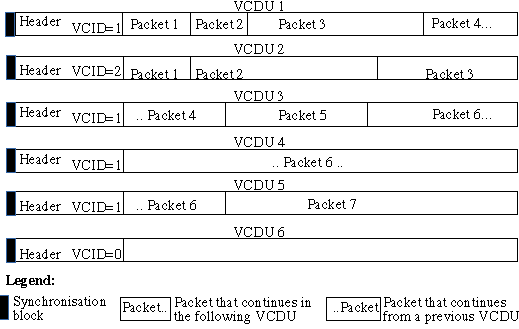
\includegraphics{images/transmissionData}
%      \caption{A simplified example of the transmission data modelled by the class diagram in Figure~\ref{fig:dataModel}.}
%      \label{fig:transmissionData}
%\end{figure}
%
%\begin{figure}[h]
%  \centering
%    \includegraphics{images/CADU}
%      \caption{Header of VCDU 3 followed by a portion of its packet zone.}
%      \label{fig:VCDU}
%\end{figure}
%
%\begin{figure}[h]
%  \centering
%    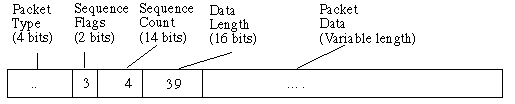
\includegraphics{images/packet}
%      \caption{Structure of a packet.}
%      \label{fig:packet}
%\end{figure}
%
%
%
%
%% An example fault model is described in Table~\ref{table:faultModel:SES}.
%%%and are used to identify the fields that can be mutated to generate new inputs.
%%For example, 
%%the two stereotypes \emph{Identifier} and \emph{Measure} are used to indicate that these attributes should be modified using mutation operators specified for identifiers and measurements.
%
%
%In the presence of UML models, constraints between inputs and outputs can be represented using OCL.
%These constraints are used as an oracle to validate the execution of automatically generated test cases: a violated constraint indicates that the system under test does not produce the expected output. 
%%The use of OCL constraints enable engineers to represent information that cannot be captured with grammars.
%%In the case of SES-DAQ, we use OCL constraints to model the error messages expected in the presence of specific faults in the input data.
%For example, Figure~\ref{fig:costraint:firstHeader} shows an OCL constraint that states that the frame count of a VCDU should be greater by one than the frame count of the previous VCDU on the same virtual channel. Otherwise, an error event \emph{COUNTER\_JUMP} should exist in the system output log file. 
%In the context of data-driven mutation testing they can be used to determine if a mutant had been killed by a test case (e.g., a constraint may capture the presence of a log entry indicting the triggering a redundancy mechanism).
%
%
%
%\begin{figure}[t!]
%\scriptsize
%\begin{tabular}{p{0.1cm}p{8cm}}
%1&\textbf{context} Vcdu \textbf{inv}:\\
%2&\textbf{let}\\
%3&\hspace{0.3cm}frameCount : Integer = self.header.vcFrameCount, \\
%4&\hspace{0.3cm}vdcuIndex : Integer = self.virtualChannel.vcdu$\rightarrow$indexOf( self ), \\
%5&\hspace{0.3cm}previous : Vcdu = self.virtualChannel.vcdu$\rightarrow$at( vcduIndex - 1 ),\\
%6&\hspace{0.3cm}previousFrameCount : Integer = previous.header.vcFrameCount\\
%7&\textbf{in} \\
%8&\hspace{0.3cm}\textbf{if} previousFrameCount $<$ 16777215 \\
%9&\hspace{0.6cm}\textbf{then} frameCount $<>$ previousFrameCount + 1 \\
%10&\hspace{0.3cm}\textbf{else} previousFrameCount $=$ 16777215 and frameCount $<>$ 0 \textbf{endif}\\
%11&\textbf{implies} \\
%12&\hspace{0.3cm}VcduEvents.allInstances()\\
%13&\hspace{1cm}$\rightarrow$exists(e $|$ e.eventType = $COUNTER\_JUMP$) \\
%\end{tabular}
%\caption{Input/output constraint for the \emph{COUNTER\_JUMP} error event.}
%\label{fig:costraint:firstHeader}
%\end{figure}
%
%
% 
%%The stereotype \emph{Derived} is used to tag class attributes that need to be derived from other attributes after every mutation, in order to prevent trivial inconsistencies (e.g. it is used to update the checksum field when other fields are mutated). 
%%The stereotypes \emph{StreamClass} and \emph{StreamAttributes} are used to automate the loading of data from bytestreams.
%% but are out of the scope of this paper (see~\cite{ICST15} for details).
%
%The main limitation of UML-based approaches is the lack of generalistic binary parsers capable of loading data as an instance of a UML class diagram. Existing approaches rely on custom parsers~\cite{di2015generating,di2015evolutionary}.
%
%\subsubsection{Data modeling with Block Models}
%
%Approaches relying on block models~\cite{PeachFuzzer,spike,pham2016model}, require that engineers specify input data according to a specific format that captures the size of specific portions of the input data. 
%For example, Spike~\cite{spike} and Peach~\cite{PeachFuzzer} require input models that specify the format of data chunks and integrity constraints.
%Figure~\ref{fig:pit} shows a portion of an example block model taken from related work~\cite{pham2016model}.
%While being effective in fuzzing programs that process weakly-structured inputs (e.g., images and protocols), these approaches become less effective for highly-structured inputs (e.g., JavaScript).
%Compared to UML-based modeling, block models provide more limited modeling capabilities, for instance, they are less effective for highly-structured inputs; however, they are often integrated into general-purpose tools that can be easily integrated in software projects~\cite{PeachFuzzer}.
%
%
%\begin{figure}[t!]
%  \centering
%    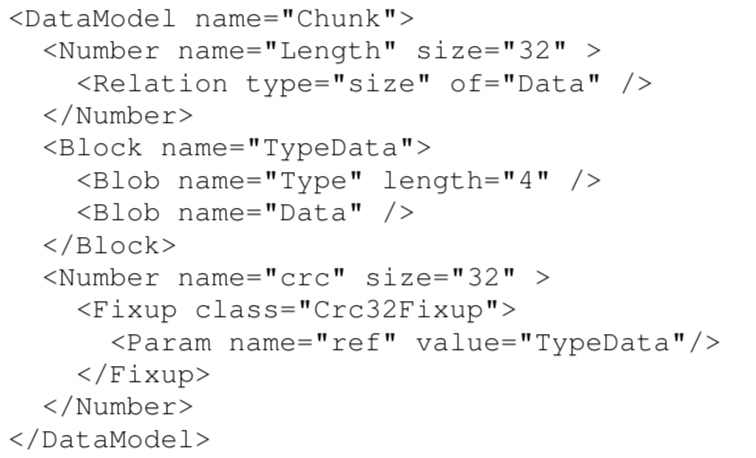
\includegraphics[width=7cm]{images/PeachPit}
%      \caption{Data model with a custom format.}
%      \label{fig:pit}
%\end{figure}
%
%
%%%%%%%%%%%%%%%%%%%%%%%%%%%%%%%%%%
%
%\subsection{Data-driven Mutation Operators}
%\label{sec:data_operators}
%
%%As mentioned in Section~\ref{sec:dataProcess}, the software engineering literature does not include any study on data-driven mutation testing but only testing approaches based on the injection of data faults.
%%For this reason, 
%In this section, we provide an overview of the fault injection techniques that have originally been developed to support software testing and can be used in the context of data-driven mutation testing. 
%More precisely, we focus on the techniques for the modification of data (hereafter, data mutation techniques) that are presented in software testing research papers.
%
%
%Table~\ref{table:dataOperators} provides an overview of groups of data mutation techniques that can be applied to space software and embedded systems. 
%We selected the set of data-driven mutation techniques in Table~\ref{table:dataOperators} based on the different types of faults commonly affecting space and embedded systems.
%Each technique aims to create data faults that might be observed in real systems either because of hardware errors or software errors.
%The data-driven mutation operators, i.e., the specific functions implemented by each technique to alter the type of data they target, are described in separate tables, in the following paragraphs. 
%%Since, for each family of technique, multiple implementations of data-driven mutation operators are available
%
%In Table~\ref{table:dataOperators}, column \emph{Name} provides the name of the specific technique described,  
% column \emph{Type of fault} indicates the type of faults each operator aims to simulate,
% column \emph{Data model} indicates if the technique requires a model of the structure of the data to be mutated,
% column \emph{Definition} provides a brief description of the technique, column \emph{Target} indicates the type of data targeted,
% column \emph{Reference} provides a reference to a research paper or tool describing the technique more in detail.
% 
%%Fabrizio: "First" and "Then" read like a story, which is not good in a Tech Report
%Concerning the type of faults considered, we focus both on hardware and software errors.
%Hardware errors are captured by the categories CPU Faults, Memory Faults, and Signal Faults. 
%Software errors are captured by the category Data Processing Faults.
%Category Communication Faults simulates problems that can be caused either by software or hardware errors.
%
%
%
%\newcommand{\FTAPE}{\cite{tsai1999stress}}
%\newcommand{\FIAT}{\cite{barton1990fault}}
%\newcommand{\GOOFI}{\cite{aidemark2001goofi}}
%\newcommand{\DOCTOR}{\cite{han1995doctor}}
%\newcommand{\ORCHESTRA}{\cite{dawson1996testing}}
%\newcommand{\Fuzz}{\cite{miller1995fuzz}}
%\newcommand{\Ballista}{\cite{koopman2000exception}}
%\newcommand{\RIDDLE}{\cite{ghosh1998testing}}
%\newcommand{\Superion}{\cite{Wang:GrammarAwareFuzzying:ICSE:2019}}
%\newcommand{\AFL}{\cite{gutmann2016fuzzing}}
%\newcommand{\SAGE}{\cite{godefroid2012sage}}
%\newcommand{\pFuzzer}{\cite{mathis2019parser}} 
%\newcommand{\MoWF}{\cite{pham2016model}}
%\newcommand{\DiNardoICST}{\cite{di2015generating}}
%\newcommand{\DiNardoASE}{\cite{di2015evolutionary}}
%\newcommand{\Matinnejad}{\cite{Matinnejad19}}
%\newcommand{\MongoDB}{\cite{Guo:MongoDBFuzzer:CACM:2017}}
%\newcommand{\SOLMI}{\cite{Jan:ISSTA:2016}}
%\newcommand{\MUSQL}{\cite{Appelt:SQLI:ISSTA:2014}}
%
%Table~\ref{table:dataMutation:references} provides the names of the tools and approaches referenced in Table~\ref{table:dataOperators}, along with a URL for the download of the tool, if available.
%
%% !TEX root =  ../MutationTestingSurvey.tex

\begin{table}[ht]
\tiny
\caption{Description of approaches and tools appearing in Table~\ref{table:dataOperators}.}
\begin{center}
\begin{tabular}{|p{1cm}|p{4cm}|p{8cm}|}
\hline
\textbf{Reference} & \textbf{Approach and Tool name} & \textbf{Available} \\
\hline

\cite{di2015evolutionary}	& Di Nardo et al. Search-based Mutation & No \\
\cite{di2015generating} & Di Nardo et al. Model-based Mutation & No \\
\cite{Matinnejad19} & Matinnejad et al. Signal Mutation & No \\

\cite{tsai1999stress} & FTAPE & No\\
\cite{barton1990fault} & FIAT & No \\
\cite{han1995doctor} & DOCTOR & No \\
\cite{dawson1996testing} & ORCHESTRA & No \\

\cite{miller1995fuzz} & Fuzz & Yes, \url{http://pages.cs.wisc.edu/~bart/fuzz/fuzz.html} \\


\cite{koopman2000exception}	&  Ballista & Yes, \url{http://users.ece.cmu.edu/~koopman/ballista/} \\

%\cite{ghosh1998testing}	& RIDDLE & No \\
\cite{Wang:GrammarAwareFuzzying:ICSE:2019} & Superion & \url{https://github.com/zhunki/Superion} \\
\MongoDB	& MongoDB Fuzzer & No \\
\SOLMI	& SOLMI &No \\
\MUSQL	& \emph{$\mu$4SQLi} &No\\
\cite{gutmann2016fuzzing} & American Fuzzy Lop & Yes, \url{https://github.com/google/AFL}\\
\cite{godefroid2012sage} & SAGE & \begin{tabular}[c]{@{}l@{}}Yes, now under Microsoft Security Risk Detection service\\\url{https://www.microsoft.com/en-us/security-risk-detection/}\end{tabular} \\
%\cite{mathis2019parser}	& pFuzzer & Yes, \url{https://github.com/uds-se/pFuzzer}\\
\cite{pham2016model} &	MoWF & No \\
\cite{spike}&SPIKE&\url{https://github.com/guilhermeferreira/spikepp}\\
\cite{PeachFuzzer}&PEACH&\url{https://www.peach.tech}\\
\cite{BooFuzz}&BooFuzz&\url{https://github.com/jtpereyda/boofuzz}\\
\hline
\end{tabular}
\end{center}
\label{table:dataMutation:references}
\end{table}%


%
%% !TEX root =  ../MutationTestingSurvey.tex

\newcommand{\FTAPE}{\cite{tsai1999stress}}
\newcommand{\FIAT}{\cite{barton1990fault}}
\newcommand{\GOOFI}{\cite{aidemark2001goofi}}
\newcommand{\DOCTOR}{\cite{han1995doctor}}
\newcommand{\ORCHESTRA}{\cite{dawson1996testing}}
\newcommand{\Fuzz}{\cite{miller1995fuzz}}
\newcommand{\Ballista}{\cite{koopman2000exception}}
\newcommand{\RIDDLE}{\cite{ghosh1998testing}}
\newcommand{\AFL}{\cite{gutmann2016fuzzing}}
\newcommand{\SAGE}{\cite{godefroid2012sage}}
\newcommand{\pFuzzer}{\cite{mathis2019parser}} 
\newcommand{\MoWF}{\cite{pham2016model}}
\newcommand{\DiNardoICST}{\cite{di2015generating}}
\newcommand{\DiNardoASE}{\cite{di2015evolutionary}}
\newcommand{\Matinnejad}{\cite{Matinnejad19}}

\begin{itemize}
	\item FTAPE tool: \cite{tsai1999stress}
	\item FIAT tool: \cite{barton1990fault}
	\item GOOFI tool: \cite{aidemark2001goofi}
	\item DOCTOR tool: \cite{han1995doctor}
	\item ORCHESTRA tool: \cite{dawson1996testing}
	\item Fuzz tool:\cite{miller1995fuzz}
	\item Ballista tool: \cite{koopman2000exception}
	\item RIDDLE tool: \cite{ghosh1998testing}
	\item American Fuzzy Lop tool: \cite{gutmann2016fuzzing}
	\item SAGE tool: \cite{godefroid2012sage}
	\item pFuzzer tool: \cite{mathis2019parser}
	\item MoWF tool: \cite{pham2016model}
	\item Di Nardo et al. Model-based Mutation tool: \cite{di2015generating}
	\item Di Nardo et al. Search-based Mutation tool: \cite{di2015evolutionary}
	\item Matinnejad et al. Signal Mutation tool: \cite{Matinnejad19}
\end{itemize}

\tiny
\setlength\LTleft{0pt}
\setlength\LTright{0pt}
\begin{longtable}{@{\extracolsep{\fill}}|p{1.5cm}|p{2cm}|p{5cm}|p{3cm}|p{1cm}|@{}}
\toprule
	\textbf{Name}	&	\textbf{Type of Fault}	&	\textbf{Definition}	&	\textbf{Target}	&	\textbf{Reference} \\
	\midrule
stuck-at-0 & CPU Faults; Memory Faults & This operator corrupts data by replacing a bit/byte/word with zero. & CPU registers; Memory registers & \FTAPE, \FIAT, \GOOFI \\
stuck-at-1 & CPU Faults; Memory Faults & This operator corrupts data by replacing a bit/byte/word with one. & CPU registers; Memory registers & \FTAPE, \FIAT, \GOOFI \\
bit flips & CPU Faults; Memory Faults; Data Processing Faults & This operator mutates data by inverting the value of each bit (i.e., replacing 0 with 1 and 1 with 0). & CPU registers: saved registers, floating point registers, the program counter, global pointer, stack pointer; Local memory; Input or output parameters of a software interface. & \FTAPE, \FIAT, \GOOFI \\
disk driver codes & Communication Faults & This operator performs data mutation by modifying the error flags of a disk driver. & I/O disk driver codes. & \FTAPE \\
set & CPU Faults; Communication Faults; Memory Faults & This operator sets the value of a bit/byte by replacing the current value with one or a user-defined bitmap. & Memory: stack, heap, global data, user code, user-defined memory location; Registers: data, stack, address, program counter, status register & \FTAPE, \FIAT, \GOOFI \\
clear & CPU Faults; Communication Faults; Memory Faults & This operator clears the value of a bit/byte by replacing the current value "v" with zero. & Memory: stack, heap, global data, user code, kernel code, user-defined memory location; Registers: data, stack, address, program counter, status register & \FTAPE, \FIAT, \GOOFI \\
toggle & CPU Faults; Communication Faults; Memory Faults & This operator toggles (i.e., sets a bit to its complement state) a bit/byte. & Memory: stack, heap, global data, user code, kernel code, user-defined memory location; Registers: data, stack, address, program counter, status register & \FTAPE, \FIAT, \GOOFI \\
lose message & Communication Faults & This operator causes a message to be lost in between two communicating components. Messages can be lost intermittently, with a probability distribution specified by the users, or alternatively, every message can be lost during a certain period. & Faulty link, Faulty direction, Single message & \DOCTOR, \ORCHESTRA \\
duplicate message & Communication Faults & This operator causes a message to be duplicated in between two communicating components. & Faulty link, Faulty direction, Single message & \DOCTOR, \ORCHESTRA \\
alter message header & Communication Faults & This operator alters a message. The change is performed in a similar manner as for memory faults, i.e., by performing bit flips. The mutation is performed in the message header. & Faulty link, Faulty direction, Single message & \DOCTOR, \ORCHESTRA \\
alter message body & Communication Faults & This operator alters a message. The change is performed in a similar manner as for memory faults, i.e., by performing bit flips. The mutation is performed in the message body. & Faulty link, Faulty direction, Single message & \DOCTOR, \ORCHESTRA \\
delay message & Communication Faults & This operator causes a message to be delayed in between two communicating components. The delay time can either be constant or follow a probability distribution. & Faulty link, Faulty direction, Single message & \DOCTOR, \ORCHESTRA \\
fuzzing & Data Processing Faults & Fuzzing techniques replace values with values (i.e., fuzz values) that are different and, usually, randomly generated. & Structured input data (e.g., files, streams) & \Fuzz, \Ballista \\
grammar-based fuzzing & Data Processing Faults & This fuzzing approach relies on a grammar that describes the format of the data to be altered; new values are generated according to the grammar. The use of the grammar decreases the chances of generating invalid inputs. & Structured input data (e.g., files, streams) & \RIDDLE \\
evolutionary fuzzing & Data Processing Faults & This fuzzing approach relies on evolutionary algorithms (e.g., genetic algorithms) to generate fuzz values. It relies on a fitness function to maximize structural coverage (e.g., branches executed during testing). The fitness is implemented by instrumenting the code of the application to collect code coverage. & Structured input data (e.g., files, streams) & \AFL \\
whitebox fuzzing & Data Processing Faults & This fuzzing approach relies on symbolic execution techniques to cover corners cases on the different execution paths. & Structured input data (e.g., files, streams) & \SAGE \\
parser-directed fuzzing & Data Processing Faults & Fuzzing techniques replace a correct value with a randomly generated one. This fuzzing operator is applied to programs that integrate a parser component to extract information from the provided inputs. It is implemented through a test generator technique that aims to produce valid inputs for the parser, the inputs are produced randomly and then checked using constraint solving techniques. & Structured input data (e.g., files, streams) & \pFuzzer \\
model-based whitebox fuzzing & Data Processing Faults & Fuzzing techniques replace a correct value with a randomly generated one, in this case, the replacement is done using a model-based whitebox fuzzing technique, the technique prunes from the search space those paths that are exercised by invalid, malformed inputs. The model should specify the format of the data chunks and integrity constraints. & Structured input data (e.g., files, streams) & \MoWF \\
data-type based injection & Data Processing Faults & This operator replaces a value with an invalid one, selected on the basis of the type of the parameter being corrupted. & Structured input data (e.g., files, streams) & \Fuzz, \Ballista, \RIDDLE \\
model-based mutation & Data Processing Faults & This approach alters existing inputs by relying on a data model that capture the structure of the data and the constraints among data fields. A predefined set of operators indicating how to alter data based on its structure are provided. & Structured input data (e.g., files, streams) & \DiNardoICST \\
search-based data mutation & Data Processing Faults & This approach alters existing inputs by relying on a data model that captures the structure of the data and the constraints between data fields. A search-based, evolutionary algorithm is used to maximize a number of mutation objectives including the number of constraints being violated and code coverage. & Structured input data (e.g., files, streams) & \DiNardoASE \\
signal mutation & Signal faults & This approach alters signal by either shifting the signal based on a randomly selected value or shifting the signal and increasing the number of signal pieces (i.e., segments).  & Input signals & \Matinnejad \\

	\bottomrule                                                             
\caption{Data-driven Mutation Operators.}
\label{table:dataOperators}
\end{longtable}
\normalsize
%
%To summarize the data in Table~\ref{table:dataOperators}, we observe that:
%\begin{itemize}
%  %Note: always put a comma at the end of a list before "or" "and"
%  \item Category CPU Faults includes techniques that perform mutations in the contents of an individual bit, byte, or word in a CPU register. The mutations in this category can target saved, floating-point, program-counter, global and stack-pointer register locations. 
%  \item Category Memory Faults includes techniques that perform mutations in the contents of an individual bit, byte, or word in a memory register. The mutations in this category can target stack, heap, global-data and user-defined memory locations.
%  \item Category Communication Faults includes techniques that simulate packet corruption faults. The mutations in this category can target channels between components, single messages, and the addresses of the messages to be exchanged.
%  \item Category Data Processing Faults includes techniques that mutate the data being processed by the system. Some of these techniques are white-box, they process the source code of the application to generate inputs more efficiently. Other techniques require a model of the data to be mutated. The mutations in this category can target both the input and the output parameters of the interface of a software component.
%  \item Category Signal Faults includes techniques that alter the shape of the signals received by the software under test.
%\end{itemize}
%
%In the following, we provide an overview of the mutation operators implemented by the most representative techniques.
%We do not present simple fuzzing approaches because they simply perform random mutations and they include a subset of the operators implemented in the more advanced evolutionary fuzzing approaches.
%
%\subsubsection{Blind memory corruption and blind transmission corruption}
%
%The mutation operators implemented by techniques performing blind memory corruption and blind transmission corruption are presented in Tables~\ref{table:operators:blindTransmissions} and ~\ref{table:operators:blindTransmissions}, respectively. These techniques do not require a data model. Unfortunately, they are of little usefulness to simulate subtle errors that affect relations among data (e.g., replacing an identifier with another legal one).
%
%%Among all the data mutation operators reported in Table~\ref{table:dataOperators}, the ones targeting \emph{Data Processing Faults} are more powerful since they concern the modification of complex data structures. %Oscar: not sure that "overviewed" is spelled right %They are briefly overviewed in the following.
%%We provide an overview in the following.
%
%
%\subsubsection{Evolutionary Fuzzing}
%
%
%%\subsubsection{Approaches generating data from scratch}
%AFL is an instrumentation-guided fuzzer~\cite{gutmann2016fuzzing}. It integrates genetic algorithms with a form of branch coverage called state transition coverage,
%which captures the number of times each branch is taken in an execution. 
%AFL aims to generate inputs that exercise all the different code paths.
%%It is implemented by executing for every instruction of the program under test the following lines
%%cur_location = <COMPILE_TIME_RANDOM>;
%%coverage[cur_location ^ prev_location]++; 
%%prev_location = cur_location >> 1;
%It requires one or more starting files that contain input data normally processed by the targeted application. 
%Each provided input is processed in a queue. For each input in the queue, AFL trims the test case to the smallest size that doesn't alter the coverage of the program. Then it repeatedly mutates the file using a set of fuzzing strategies, which are presented in Table~\ref{table:AFL:operators}.
%If any of the generated mutations result in a change of the coverage for the software under test, the mutated input is added to the input queue.
%
%% !TEX root =  ../MutationTestingSurvey.tex

%
%\setlength\LTleft{0pt}
%\setlength\LTright{0pt}
%\begin{longtable}{@{\extracolsep{\fill}}|p{2.5cm}|p{5cm}|p{5cm}|@{}}
%\toprule


\begin{table}[h]
\caption{Mutation Operations performed by AFL~\cite{gutmann2016fuzzing}}
\label{table:AFL:operators}


\tiny
\begin{tabular}{|p{2.5cm}|p{10cm}|}

\hline

\textbf{Walking bit flips}& Sequential, ordered bit flips. The number of bits flipped in a row varies from one to four in steps of two. This strategy is applied till the coverage of the program under test does not change.\\

\hline
\textbf{Walking byte flips}& This method relies on 8-, 16-, or 32-bit wide bitflips with a constant stepover of one byte. \\

\hline
\textbf{Simple arithmetics}& Increment and decrement existing integer values in the input file; this is done considering every byte of the file. The chosen range for the operation is -35 to +35. It is performed in three steps. First, the fuzzer attempts to perform subtraction and addition on individual bytes. The second steps involves looking at 16-bit values, using both endians - but incrementing or decrementing them only if the operation has affected the most significant byte. The final stage follows the same logic, but for 32-bit integers.\\

\hline
\textbf{Known integers}& 
AFL overwrites every byte in the input file with a set of interesting values (e.g., -1, 256, 1024, MAX\_INT-1, MAX\_INT), using both endians (the writes are 8-, 16-, and 32-bit wide).\\

\hline
\textbf{Stacked tweaks}& Sequence of randomly selected mutations among the following: Single-bit flips, Attempts to set "interesting" bytes, words, or dwords (both endians), Addition or subtraction of small integers considering bytes, words, or double words (both endians), Random single-byte sets, Block deletion, Block duplication via overwrite or insertion, Block memset. \\

\hline
\textbf{Test case splicing}& Consists of taking two distinct input files that differ in at least two locations, splicing them at a random location in the middle, and then applying stacked tweaks.\\

\hline
%\bottomrule                                                             

\end{tabular}
\end{table}
%\normalsize



%
%\subsubsection{Grammar-based fuzzing}
%
%Superion~\Superion~ extends \emph{AFL} to drive mutations based on grammars. It takes as input an ANTLR~\cite{ANTLR} grammar. 
%It performs mutations that consist of grammar-aware trimming, dictionary-based mutations, and tree-based mutation.
%Grammar-aware trimming is performed by generating an AST tree from the input and by deleting a randomly-selected subtree. 
%It aims to generate trimmed inputs that do not alter code coverage in the SUT.
%Dictionary-based mutations are performed by building a dictionary using every token in the input file and by inserting the elements of the dictionary in the boundaries of every token in the input file.
%Tree-based mutation is performed by processing two input files and replacing the subtrees of one file with the ones of another.
%Listing~\ref{mutatedJSONfile} shows a JSON file generated by deleting a randomly-selected subtree from Listing~\ref{JSONfile}.
%
%
\begin{minipage}{14cm}
\footnotesize
\begin{lstlisting}[caption=JSON file generated by deleting a subtree from Listing~\ref{JSONfile}., label=mutatedJSONfile]
{
 [
 {
  "firstName": "Fabrizio",
  "lastName": "Pastore",
  "isAlive": true,
  },
  {
  "firstName": "Oscar",
  "lastName": "Cornejo",
  "isAlive": true,
  "address": {
    "streetAddress": "29, Avenue J.F Kennedy",
    "city": "Luxembourg",
    "state": "Luxembourg",
    "postalCode": "L-1855"
  },
  }
  ]
}
\end{lstlisting}
\end{minipage}
%
%%Fabrizio: you had this definition of equivalent: "(i.e., correct fuzzed data, but semantically meaningless)." it is difficult to understand
%
%
%%Fabrizio: I cannot understand the following sentences
%%Although it tackles the problem of redundant mutants by well covering the space of possible inputs, it does not tackle the redundant mutant problem.
%%Cannot handle semantic restrictions imposed by certain nontrivial input languages. The approach has difficulties to handle complex sequences recursion.
%
%%\subsubsection{Approaches altering existing data}
%
%
%\emph{$\mu$4SQLi}~\cite{Appelt:SQLI:ISSTA:2014} relies on a SQL grammar to generate SQL injections. 
%SQL injections are generated by means of a set of mutation operators, shown in Table~\ref{table:Mu4SQLI}, that alter the values of an input according to predefined patterns.
%Similarly, SOLMI~\cite{Jan:ISSTA:2016} relies on the XML grammar to alter XML messages based on a predefined set of mutation operators and introduce potential XML injections. 
%SOLMI implements four operators that (1) introduce XML meta-characters, (2) introduce closing tags, (3) replicate XML elements, (4) replace XML content.
%
%
%\begin{table}[h]
%\caption{Mutation operators implemented by $\mu$4SQLi}
%\label{table:Mu4SQLI}
%\begin{tabular}{|p{2cm}|p{11.5cm}|}
%\hline
%\multicolumn{2}{|c|}{Behaviour-Changing Operators}\\
%\hline
%MO\_or&Adds an OR-clause to the input\\
%MO\_and&Adds an AND-clause to the input\\
%MO\_semi&Adds a semicolon followed by an additional SQL statement\\
%\hline
%\multicolumn{2}{|c|}{Syntax-Repairing Operators}\\
%\hline
%MO\_par&Appends a parenthesis to a valid input\\
%MO\_cmt&Adds a comment command (- - or \#) to an input\\
%MO\_qot&Adds a single or double quote to an input\\
%\hline
%\multicolumn{2}{|c|}{Obfuscation Operators}\\
%\hline
%MO\_wsp&Changes the encoding of whitespaces \\
%MO\_chr&Changes the encoding of a character literal enclosed in quotes\\
%MO\_html&Changes the encoding of an input to HTML entity encoding\\
%MO\_per&Changes the encoding of an input to percentage encoding\\
%MO\_bool&Rewrites a boolean expression while preserving its truth value\\
%MO\_keyw&Obfuscates SQL keywords by randomising the capitalisation and inserting comments\\
%\hline
%\end{tabular}
%\end{table}
%
%
%Tal et al.~\cite{Tal2004} presented a syntax-based vulnerability testing technique based on mutations of ASN.1 grammars. The objective is to detect software vulnerabilities detecting anomalous behavior or crashes in the SUT (e.g., segmentation faults, buffer, heap or stack overflows, etc.) when parsing mutated PDUs. The PDUs are specified by frames (data structures), which explicitly defines the order of data fields in the PDU, as well as the exact length of each field. 
%The proposed approach intercepts OSPF packets and translates it to a TXL readable file, then the mutations are applied to ASN.1 syntax contained in the TXL file. The mutation strategies applied are the following: \textbf{replacement} (replacing one field at a time with boundary and mid-way values), \textbf{removal} (removing one field at a time, and then removing pairs of fields, one pair at a time), and \textbf{permutation} (permutating pairs of fields within each SEQUENCE and SET).
%
%% \textbf{Syntax-based Vulnerability Testing of Frame-based Network Protocols}
%% \cite{Tal2004} The paper presents a syntax-based vulnerability testing technique based on mutations of Protocol Data Units (PDU) performed on the ASN.1 syntax. The objective is to detect software vulnerabilities detecting anomalous behavior or crashes in the SUT (e.g., segmentation faults, buffer, heap or stack overflows, etc.) when parsing mutated PDUs. The PDUs are specified by frames (data structures), which explicitly defines the order of data fields in the PDU, as well as the exact length of each field.
%% Syntax is specified in BNF notation, mutations are then made to the syntactic elements and the grammar is used to produce mutated vectors (PDUs). In the paper, the transferred packets are based on the OSPF protocol. Previously, it has been applied to WAP, HTTP, LDAP and SNMP protocols.
%% The proposed approach intercepts a packet and translates it to a TXL readable file, then the mutations are applied to ASN.1 syntax contained in the TXL file. The mutation strategies applied are the following: replacement (replacing one field at a time with boundary and mid-way values), removal (removing one field at a time, and then removing pairs of fields, one pair at a time), and permutation (permutating pairs of fields within each SEQUENCE and SET).
%
%
%% \textbf{CMM: A combination-based mutation method for SQL injection}
%
%Instead, Zhao et al.~\cite{Zhao2020} presented a mutation-based fuzzing technique for eliminating SQLi vulnerabilities. The technique is called Combinatorial Mutation Method (CMM), which mixes combinatorial testing with fuzzing techniques to generate test sets for SQLi. 
%
%The mutations are based on the mutation methods from sqlmap (open source penetration testing tool that automates the process of detecting and exploiting SQLi flaws). The authors classifies the mutation methods provided by sqlmap in five groups:
%
%
%\begin{table}[h!]
%\begin{center}
%\begin{tabular}{|p{2cm}|p{10cm}|}
%\hline
%\textbf{Fault}&\textbf{Description}\\
%\hline
%comment & attach a sql comment command at the back of an input test case.\\
%stringtamper & changes the appearance of an input, making it look valid but still malicious. \\
%space2 & changes the space character in the input.\\
%apostle& changes the apostle in the input.\\
%encoding& this kind of mutation method changes the encoding of the original statement.\\
%\hline
%\end{tabular}
%\end{center}
%\caption{Fault Model from \cite{Zhao2020}}
%\label{table:faultModel:Zhao2020}
%\end{table}%
%
%The test set is created by using combinatorial testing on the different inputs created by the mutation tool.
%
%
%
%%\textbf{Testing for software vulnerability using environment perturbation}
%
%Du et al.~\cite{Du2002} introduced a fault injection technique to perform environment perturbations for testing a software system for possible security flaws. The paper introduces a fault model called Environment-Application Interaction (EAI).
%
%Given the assumption that a system is composed of an application plus its environment, in the paper faults are injected into the environment thereby perturbing it, the idea is to verify if the program responds and whether there will be a security violation under this perturbation, otherwise the system is considered secure.
%
%The faults are injected at the points where the environment and the application interact. The environment faults becomes faults in the input, which is then inherited by an internal entity of the application. From this point onwards the environment faults propagate through the application via the internal entities. If the application does not handle the faults correctly, a security violation might occur. The direct reason for this violation appears to be faults in the internal entity. 
%Authors classify environment faults in two categories: (1) indirect: affect programs via internal entities (primary sources of program inputs). (2) direct: affect programs via environment faults.
%
%
%\begin{figure}[h]
%  \centering
%    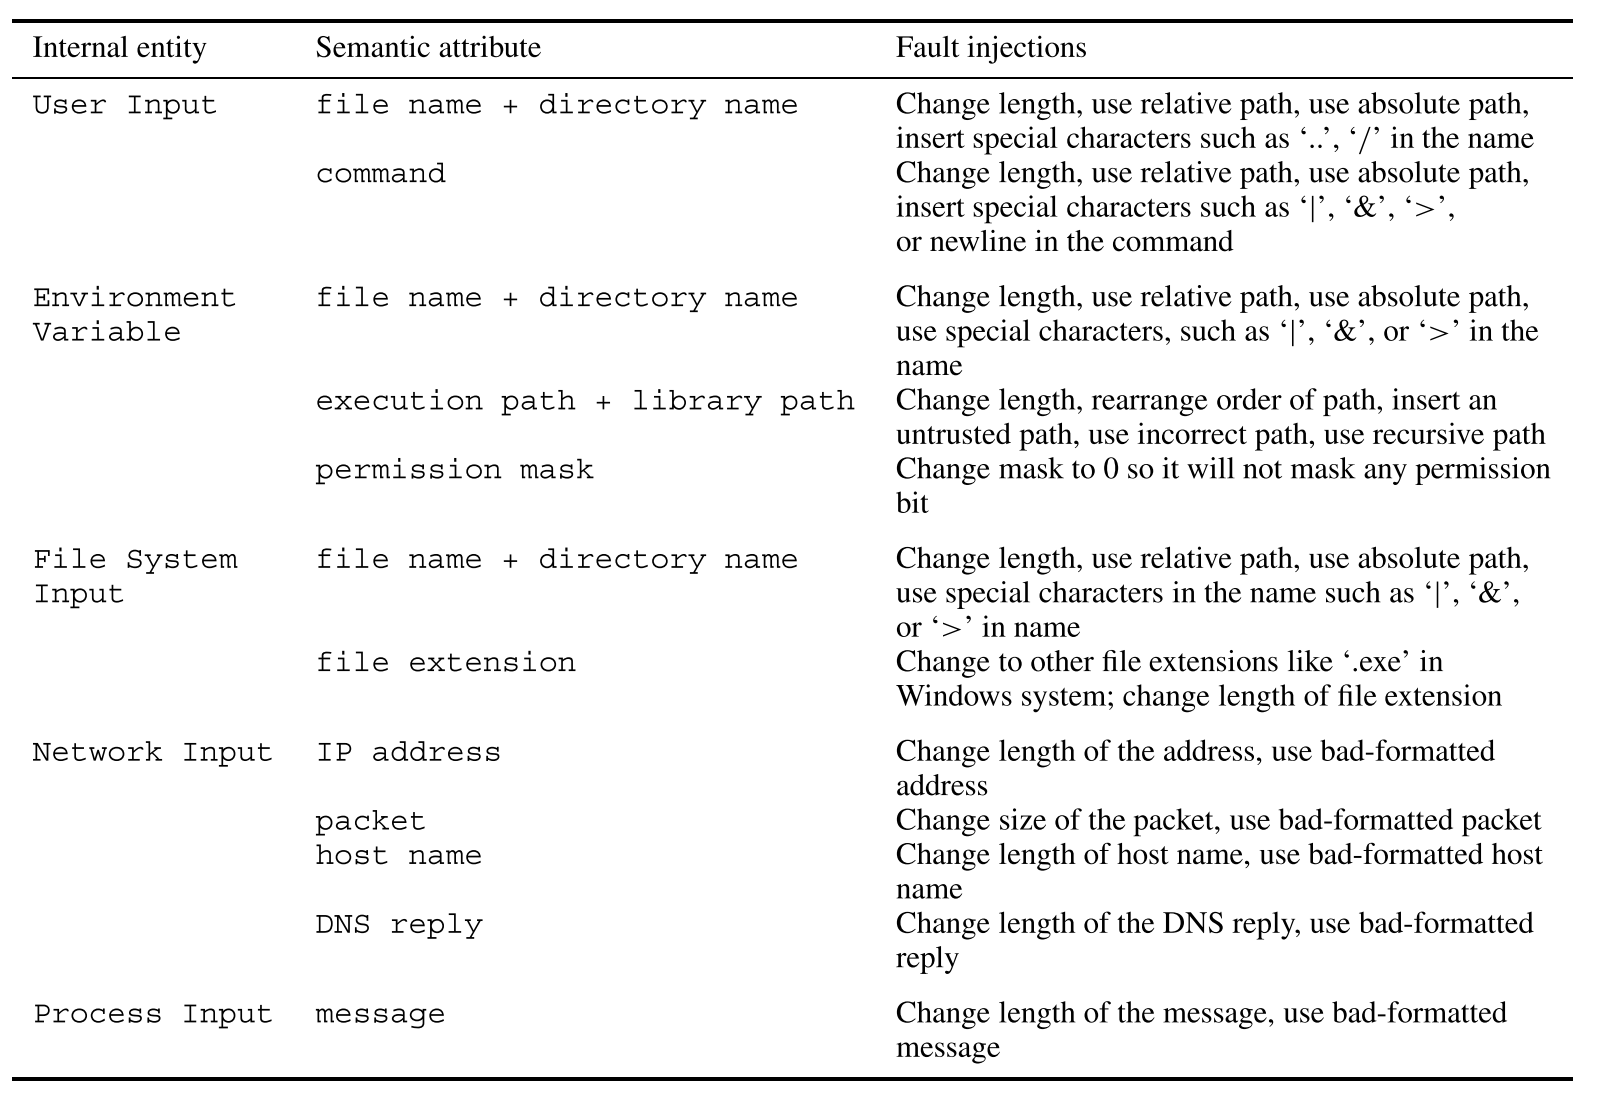
\includegraphics[width=0.8\textwidth]{images/du2002a}
%      \caption{Indirect environment faults and environment perturbations operators.}
%\end{figure}
%
%
%\begin{figure}[h]
%  \centering
%    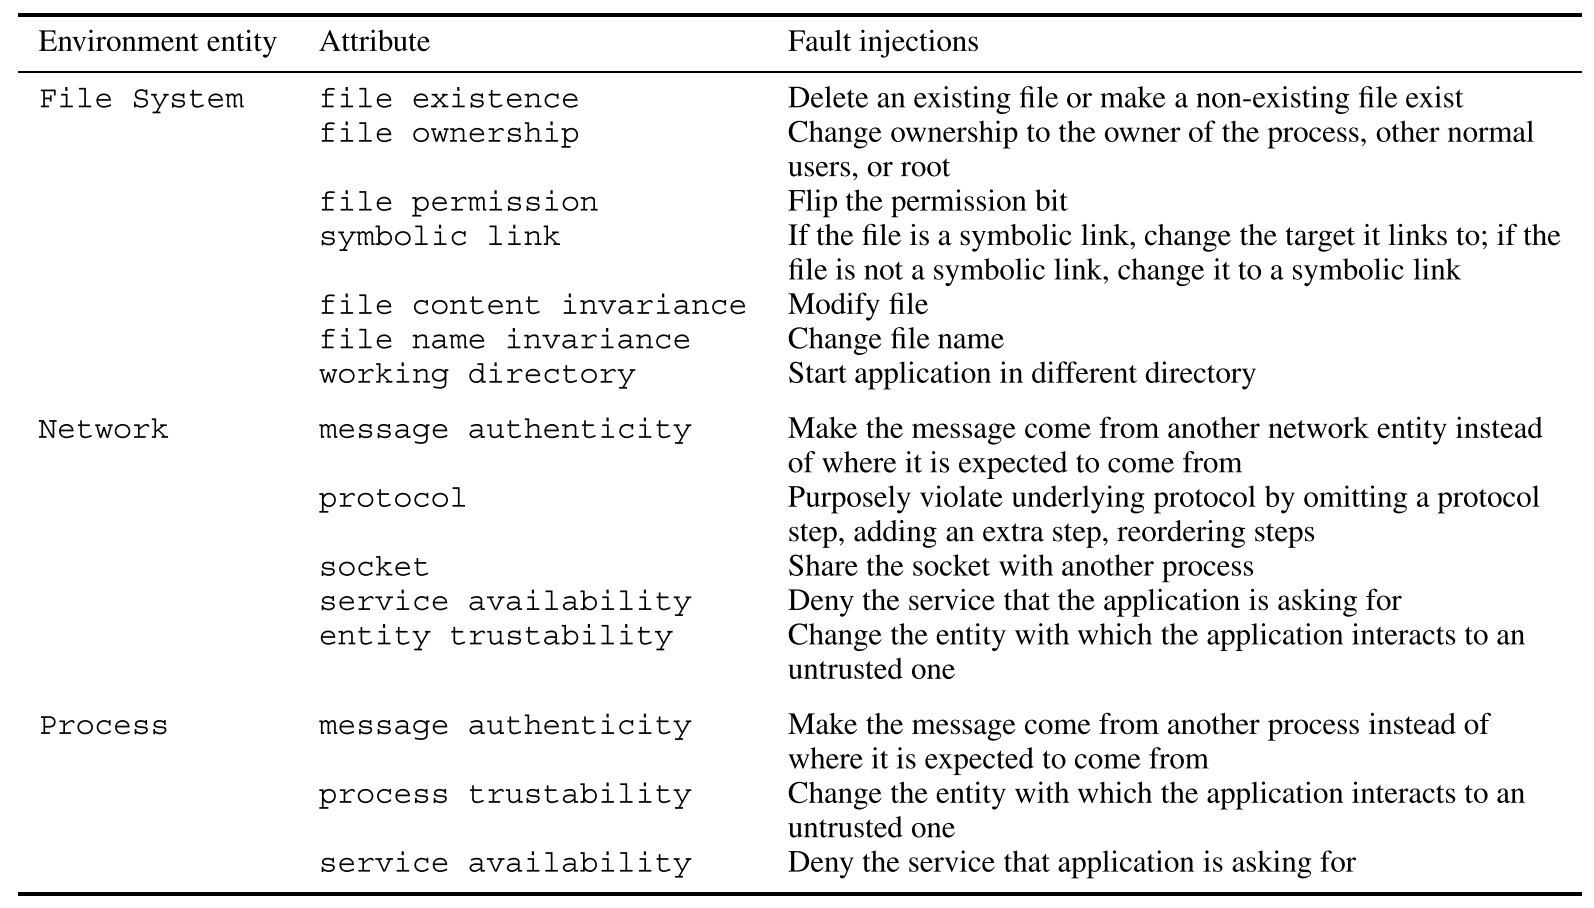
\includegraphics[width=0.8\textwidth]{images/du2002b}
%      \caption{direct environment and environment perturbations operators.}
%\end{figure}
%
%They use fault coverage (percentage of the number of faults tolerated to the faults injected) and interaction coverage (percentage of the number of interaction points where faults are injected w.r.t to total of interaction points) to measure the test adequacy.
%
%
%
%One of the major limitations of grammar-based approaches is the cost of defining an input grammar. MongoDB's javascript fuzzer addresses the problem of grammar-based mutation when a grammar is not available. Instead of mutating input files for the SUT based on the input grammar of  the SUT, it mutates test cases for the SUT (in this case the Javascript test cases)~\MongoDB. It replaces subtrees in the AST tree generated from the test cases either other subtrees belonging to the same input file or with subtrees generated following encoded production rules.
%
%
%
%
%
%\subsubsection{Whitebox fuzzing}
%
%%, also, it requires more knowledge about the target than purely random ones.
%
%SAGE adopts symbolic execution to systematically generate malformed inputs~\cite{godefroid2012sage}. SAGE performs fuzzing on file- and packet-parsing applications. 
%The program is first executed with concrete inputs; in order to identify a set of constraints on inputs, then, one of the constraints in the set is negated, and new malformed inputs are generated to satisfy the new set of constraints. 
%The main benefit of SAGE is that it forces the program to execute corner cases not covered by the initial inputs; for example, 
%%Fabrizio: you wrote the following, which I could not understand please check if my sentence is correct
%%(e.g., reached one-third of all bugs found by fuzz testing in Microsoft projects \cite{bounimova2013billions}).
%%Oscar: yes, what you wrote is correct 
%one-third of all the bugs found by means of fuzz testing are detected thanks to SAGE \cite{bounimova2013billions}.
%Unfortunately, the main limitation of SAGE and symbolic execution-based fuzzers is its limited scalability, due to the high execution time required by symbolic execution.
%
%%Fabrizio: not sure what the following is about, ignoring
%%\emph{Testing of Fault-Tolerant and Real-Time Distributed Systems via Protocol Fault Injection \cite{dawson1996testing}}: The paper introduces a portable fault injection environment for testing implementations of distributed protocols.
%
%\subsubsection{Model-based fuzzing}
%
%%Fabrizio: we miss the pro/cons from the following
%Model-based fuzzing targets program binaries that process structured inputs.
%Model-Based Blackbox Fuzzing (MoBF) is performed using block models that capture the structure of the input data for the SUT. A solution to perform MoBF is Peach~\cite{PeachFuzzer,PeachMozilla}, which alters data of an input files according to a large, predefined set of rules. We provide an overview of the mutation operators implemented by Peach in Table~\ref{table:PeachOperators}.
%Model-Based Whitebox Fuzzing, instead, relies on additional information about code coverage to generates valid inputs that exercise critical target locations~\cite{pham2016model}. This is done through a directed path exploration technique that prunes from the search space those paths that are exercised by invalid, malformed inputs.
%Compared with a Model-Based Blackbox Fuzzer (MoBF) approach, the \emph{MoWF} prototype was able to expose all of 13 vulnerabilities on an empirical evaluation carried on nine subject programs, while the MoBF approach only detected 6 out of 13 vulnerabilities. 
%
%% !TEX root = ../MutationTestingSurvey.tex

\begin{table}[h]
\begin{center}
\footnotesize
\CHANGEDTWO{
\begin{tabular}{|p{5cm}|p{9cm}|}
\hline
\textbf{Operator Name}&\textbf{Description}\\
\hline
ArrayVarianceMutator&Change the length of arrays. Given L the original length of the array, the length is changed in range L-N to L+N.\\
ArrayReverseOrderMutator&Reverse the order of an array.\\
ArrayRandomizeOrderMutator&Put array elements in random order.\\
DWORDSliderMutator&Slides a DWORD through the blob.\\
BitFlipperMutator&Flips a given \% of bits in blob. Default is 20\%.\\
BlobMutator&Randomly grows a Blob block or shrinks it.\\
DataTreeRemoveMutator&Remove nodes from data tree.\\
DataTreeDuplicateMutator&Duplicate a node's value starting at 2x through 50x.\\
DataTreeSwapNearNodesMutator&Swap the data of two nodes that are near each other in the data model.\\
NumericalVarianceMutator&Produce numbers that are defaultValue - N to defaultValue + N.\\
NumericalEdgeCaseMutator&Replace with random numbers of appropriate correct size.\\
FiniteRandomNumbersMutator&Produce a finite number of random numbers for each \emph{Number} element.\\
NumericalEvenDistributionMutator&Generate numbers evenly distributed through the total numerical space of the number range.\\
NullMutator&Does nothing, just test the data produced by the fuzzer.\\
PathValidationMutator&Does not mutate. Used to trace path of each test for path validation.\\
SizedVarianceMutator&Change the length of sizes to count - N to count + N.\\
SizedNumericalEdgeCasesMutator&Change the length of sizes to numerical edge cases.\\
SizedDataVarianceMutator& Change the length of sized data to count - N to count + N. Size indicator will stay the same.\\
SizedDataNumericalEdgeCasesMutator&Change the length of sizes to numerical edge cases.\\
StringCaseMutator&Change the case of a string.\\
UnicodeStringsMutator&Generate unicode strings.\\
ValidValuesMutator&Replace with random values other than the legal ones.\\
UnicodeBomMutator&Injects BOM markers into default value and longer strings.\\
UnicodeBadUtf8Mutator&Generate bad UTF-8 strings.\\
UnicodeUtf8ThreeCharMutator&Generate long UTF-8 three byte strings.\\
StringMutator&Generate a random unicode string, for each string node, one Node at a time.\\
XmlW3CMutator&Replace XML trees with invalid, non-well former, and valid (but random) XML trees.\\
PathMutator&Replace a path with an erroneous path generated according to 20 different rules.\\
HostnameMutator&Replace a hostname with an erroneous hostname generated according to 20 different rules.\\
IpAddressMutator&Replace an IP address with an erroneous IP address generated according to 20 different rules.\\
TimeMutator&Replace a time value with an erroneous value generated according to 3 different rules.\\
DateMutator&Replace a date with 60 predefined erroneous dates.\\ 
FilenameMutator&Replace a file name with an file name generated according to 10 different rules.\\
ArrayNumericalEdgeCasesMutator&This operator is not well documented in the source code of Peach.\\
BlobSpread&This operator is not well documented in the source code of Peach.\\
\hline
\end{tabular}
}
\end{center}
\caption{Mutation Operators for the opensource version of Peach~\cite{PeachMozilla}}
\label{table:PeachOperators}
\end{table}%
%
%\subsubsection{Model-based data mutation}
%
%%\emph{Generating complex and faulty test data through model-based mutation analysis (Research paper) \cite{di2015generating}}: 
%Model-based data mutation testing concerns the automated generation of invalid input data through the mutation of existing data based on a predefined set of mutation operators~\cite{di2015generating}.
%The technique receives two inputs: field data and a data model, i.e., a UML class diagram annotated with stereotypes and OCL constraints. 
%An example data model has been shown in Figure~\ref{fig:dataModel} while an example OCL constraint appears in Figure~\ref{fig:costraint:firstHeader}. 
%The technique relies upon six generic mutation operators to automatically generate faulty data. 
%Table~\ref{table:dataModelMutationOperators} provides an overview of the mutation operators proposed in ~\cite{di2015generating}.
%In model-based data mutation~\cite{di2015generating} stereotypes are used to tailor the behaviour of the generic mutation operators to the fault model for the system under test and the environment in which it is deployed. 
%Table~\ref{table:faultModel:SES} shows a fault model for a satellite system that processes the data presented in Figure~\ref{fig:dataModel}.
%Mutation operators are applied to the data according to the stereotypes used in the data model.
%Table~\ref{table:mapping} shows the mutation operators and the corresponding stereotypes. In~\cite{di2015generating}, the mutation operator \emph{Attribute Bit Flipping} is applied on all the attributes not tagged with other stereotypes. 
%
%\begin{table}[h]
\begin{center}
\begin{tabular}{|p{5cm}|p{5cm}|p{2.5cm}|}
\hline
\textbf{Fault}&\textbf{Mutation Operator}&\textbf{Stereotype}\\
\hline
Duplicate VCDU/Packet& Class Instance Duplication.&InputData\\
Missing VCDU/Packet& Class Instance Removal.&InputData\\
Wrong Sequence& Class Instances Swapping.&InputData\\
Incorrect Identifier& Attribute Replacement with Random.&Identifier\\
Incorrect Checksum& Attribute Replacement with Random.&Identifier\\
Incorrect Counter& Attribute Replacement using Boundary Condition.&Measure\\
Flipped Data Bits& Attribute Bit Flipping.&\\
\hline
\end{tabular}
\end{center}
\caption{Mapping between Fault Data and Mutation Operators in \cite{di2015generating}.}
\label{table:mapping}
\end{table}%
%
%% !TEX root =  ../MutationTestingSurvey.tex

%
%\setlength\LTleft{0pt}
%\setlength\LTright{0pt}
%\begin{longtable}{@{\extracolsep{\fill}}|p{2.5cm}|p{5cm}|p{5cm}|@{}}
%\toprule


\begin{table}[h]
\caption{Mutation Operators for Model-based Data-driven Mutation Testing. Based on~\cite{di2015generating}}
\label{table:dataModelMutationOperators}


\tiny
\begin{tabular}{|p{2.5cm}|p{5cm}|p{7cm}|}

\hline
\textbf{Operator}&\textbf{Description}&\textbf{Example}\\
\hline
\textbf{Class Instance Duplication (CID)}&
The operator \emph{Class Instance Duplication} duplicates an instance of a class belonging to a collection of elements. This operator copies a randomly chosen instance of a class in a collection and then inserts it at a random position in the collection. This operator simulates unexpected data in a collection.
&In Figure~\ref{fig:dataModel}, this operator can be applied to the associations between the classes \emph{Transmission} and \emph{Vcdu}, and between the classes \emph{VirtualChannel} and \emph{Packet}. In both cases the duplicated data generated by this operator simulates a transmission error.\\
\hline
\textbf{Class Instance Removal (CIR)}
&This mutation operator deletes a randomly selected instance of a class from a collection of elements. 
&In Figure~\ref{fig:dataModel}, this operator can be applied to the associations between the classes \emph{Transmission} and \emph{Vcdu}, and between the classes \emph{VirtualChannel} and \emph{Packet}. The removal of an instance of class \emph{Vcdu}, for example, simulates a transmission error that may lead to either missing or broken Packets. When processing erroneous data created with this mutation operator, SES-DAQ should report a \emph{COUNTER\_JUMP} error as indicated by the constraint in Figure~\ref{fig:costraint:firstHeader}. \\
\hline
\textbf{Class Instances Swapping (CIS)}
&Swaps the positions of two randomly chosen instances of a class in a collection of elements. 
&In Figure~\ref{fig:dataModel}, this operator can be applied to the associations between the classes \emph{Transmission} and \emph{Vcdu}, and between the classes \emph{VirtualChannel} and \emph{Packet}. The effect of swapping two packets belonging to the association between the classes \emph{VirtualChannel} and \emph{Packet} simulates the presence of transmission data sequence errors.\\
\hline

\textbf{Attribute Replacement with Random (ARR)}
&This mutation operator replaces the value of an identifier attribute in an instance of a class with a randomly chosen value. In principle all the attributes of a class can be replaced with randomly chosen values, but in the general case a randomly generated value is not necessarily erroneous.
We are interested in mutations that lead to errors, 
for this reason we introduced the UML stereotype $Identifier$ that allows software engineers to indicate which attributes are used as identifiers, and thus can be mutated according to the ARR operator. The $Identifier$ stereotype enables software engineers to specify a numeric range for the random value to generate.
&In Figure~\ref{fig:dataModel}, this mutation operator can be applied to all the attributes tagged with the stereotype \emph{Identifier}. For example a random mutation of the attribute \emph{versionNumber} belonging to an instance of class \emph{Header} simulates an invalid frame version, which should be reported by the software. 
\\
\hline
\textbf{Attribute Replacement using Boundary Condition (ARBC)}
& This mutation operator changes the value of an attribute according to a boundary condition criterion. This operator is particularly useful for mutating attributes that should be bound within a range, these attributes are usually measures. We thus introduced the UML stereotype \emph{Measure} to tag the attributes that belong to this category. This stereotype enables software engineers to indicate the minimum and maximum values allowed for the tagged attribute. The mutation operator generates four values out of range according to traditional boundary testing strategies: minimum value, minimum value minus one, maximum value, and maximum value plus one. The operator ensures that the generated value is in the range representable with the data type (e.g. unsigned bytes cannot represent negative values).
&In Figure~\ref{fig:dataModel}, this operator can be applied to all the attributes tagged with the UML stereotype \emph{Measure}. In the running example this operator can be applied to the attribute \emph{vcFrameCount} of class \emph{Header}. 
\\
\hline
\textbf{Attribute Bit Flipping (ABF)}
&This operator randomly selects an attribute that corresponds to transmitted data and alters the value of a randomly selected bit. This mutation operator is particularly effective for introducing errors in attributes that cannot be tagged as Identifiers or Measures.
The operator works by flipping a single bit of an attribute. 
&In Figure~\ref{fig:dataModel}, this mutation operator can be applied to the attribute \emph{packetData} of class \emph{Packet} of the running example.
The attribute \emph{packetData} is a byte array: the mutation of one of its bits
simulates the presence of a realistic transmission error that should be identified thanks to the presence of a redundancy check code.
\\
\hline



%\bottomrule                                                             

\end{tabular}
\end{table}
%\normalsize
%
%% !TEX root = ../MAIN.tex
\begin{table}[h]
\begin{center}
\scriptsize
\begin{tabular}{|p{2cm}|p{2cm}|p{4cm}|p{6cm}|}
\hline
\textbf{Fault Class}&\textbf{Types}&\textbf{Parameters}&\textbf{Description}\\
\hline
Value above threshold (VAT)&
\begin{minipage}{6cm}
INT\\
LONG INT\\
FLOAT\\
DOUBLE
\end{minipage}
&
\begin{minipage}{6cm}
T: threshold\\
D: delta with respect to threshold\\
\end{minipage}
&
\begin{minipage}{6cm}
The value is above a threshold T for a delta D. 

\EMPH{Data mutation operation:} The mutation is performed by replacing the current value (a number) with a value of the same type that is equal to $(T+D)$.
\end{minipage}
\\

\hline
Value below threshold (VBT)&
\begin{minipage}{6cm}
INT\\
LONG INT\\
FLOAT\\
DOUBLE
\end{minipage}
&
\begin{minipage}{6cm}
T: threshold\\
D: delta with respect to threshold\\
\end{minipage}
&
\begin{minipage}{6cm}
The value is below a threshold T for a delta D. 

\EMPH{Data mutation operation:} The mutation is performed by replacing the current value (a number) with a value of the same type that is equal to $(T-D)$.
\end{minipage}
\\



\hline
Value out of range (VOR)&
\begin{minipage}{4cm}
INT\\
LONG INT\\
FLOAT\\
DOUBLE
\end{minipage}
&
\begin{minipage}{4cm}
MIN: minimum valid value\\
MAX: maximum valid value\\
D: delta with respect to minimum/maximum valid value
\end{minipage}
&
\begin{minipage}{6cm}
The value is out of the valid range MIN-MAX. 

\EMPH{Data mutation operations (2):}  The mutation is performed by replacing the current value (a number) with 
\begin{itemize}
\item a value of the same type that is equal to $(MIN-D)$
\item a value of the same type that is equal to $(MAX+D)$
\end{itemize}
\end{minipage}
\\

\hline
Bit flip (BF)&
BIN
&
\begin{minipage}{4cm}
MIN: lower bit\\
MAX: higher bit\\
STATE: mutate only if the bit is in the given state\\
\TRFOUR{VALUE: integer specifying the number of bits to mutate}\\
\end{minipage}
&
\begin{minipage}{6cm}
A number of bits randomly chosen in the positions between MIN and MAX (included) are flipped.

\EMPH{Data mutation operation:} the operator flips N randomly selected bit.
If STATE is specified, the mutation is applied only if  the bit is in the specified state. Parameter VALUE specifies the number of bits to mutate.
\end{minipage}
\\

\hline
Invalid numeric value (INV)&
\begin{minipage}{6cm}
INT\\
LONG INT\\
FLOAT\\
DOUBLE
\end{minipage}
&
\begin{minipage}{4cm}
MIN: lower valid value\\
MAX: higher valid value\\
\TRFOUR{D: distribution to follow}\\
\TRFOUR{VALUE: mean value for normal distribution}\\
\end{minipage}
&
\begin{minipage}{6cm}
The value is legal (i.e., in the specified range) but different than the current one, which, in this case, is expected to be consistent with the status of the system.

\EMPH{Data mutation operation:} Mutation is performed by replacing the current value with a different value randomly sampled in the specified range. The parameter D specified the distribution to follow when performing the mutation\footnote{In our implementation 0 indicates uniform, 1 indicates normal around the specified value (but in range).}
\end{minipage}
\\

\hline
Illegal Value (IV)
&
\begin{minipage}{6cm}
INT\\
LONG INT\\
FLOAT\\
DOUBLE
\end{minipage}
&
\begin{minipage}{6cm}
VALUE: illegal value that is observed\\
\end{minipage}
&
\begin{minipage}{6cm}
The value is illegal and equal to the provided one (i.e., parameter \emph{VALUE}).

\EMPH{Data mutation operation:} Mutation is performed by replacing the current value with the value \emph{VALUE}, if different than the current one.
\end{minipage}
\\

\hline
\TRFOUR{Anomalous Signal Amplitude (ASA)}
&
\begin{minipage}{6cm}
INT\\
LONG INT\\
FLOAT\\
DOUBLE
\end{minipage}
&
\begin{minipage}{6cm}
T: change point\\
D: delta to add/remove\\
V: value to multiply\\
\end{minipage}
&
\begin{minipage}{6cm}
The value is modified by amplifying/reducing it by a factor V and adding or removing D from the observed value. It is used to "amplify" a signal in a constant manner to simulate unusual signal. T indicates the observed value below which instead of adding  we subtract .

\EMPH{Data mutation operation:} Mutation is performed by replacing the current value ($v$) with the value ($v'$) computed as follows:

\[
v' =  
    \begin{cases}
      T+(  (v-T)*V  ) + D   & \mathit{if}\ v \ge T\\
      T - (  (T-v)*V  ) - D   & \mathit{if}\ v < T
    \end{cases}       
\]
\end{minipage}
\\


\hline
\TRFOUR{Signal Shift (SS)}
&
\begin{minipage}{6cm}
INT\\
LONG INT\\
FLOAT\\
DOUBLE
\end{minipage}
&
\begin{minipage}{6cm}
D: delta by which the signal should be shifted\\
\end{minipage}
&
\begin{minipage}{6cm}
The value is modified by adding a value D. It simulate an anomalous shift in the signal.
\end{minipage}
\\





\hline
\TRFOUR{Hold Value (HV)}
&
\begin{minipage}{6cm}
BIN\\
INT\\
LONG INT\\
FLOAT\\
DOUBLE
\end{minipage}
&
\begin{minipage}{6cm}
V: number of times to repeat the same value\\
\end{minipage}
&
\begin{minipage}{6cm}
This operator keeps repeating an observed value for $V$ times. It emulates a constant signal replacing a signal supposed to vary.
\end{minipage}
\\



\hline
\TRFOUR{Array Swap (AS)}
&
\begin{minipage}{6cm}
ARRAY\_*\\
\end{minipage}
&
\begin{minipage}{6cm}
MIN: position of element A\\
MAX: position of element B\\
VALUE: number of elements to move\\
\end{minipage}
&
\begin{minipage}{6cm}
Replace a number of elements (number specified by VALUE) located starting from position MIN, with a number of elements located starting from position MAX, and viceversa.
\EMPH{Data mutation operation:} Mutation is performed by replacing the two set of elements with each other.
\end{minipage}
\\


\hline
\TRFOUR{Array Random Swap (ARS)}
&
\begin{minipage}{6cm}
ARRAY\_*\\
\end{minipage}
&
\begin{minipage}{6cm}
MIN: min position of element A/B\\
MAX: max position of element A/B\\
VALUE: number of elements to move\\
\end{minipage}
&
\begin{minipage}{6cm}
Replace a number of elements (number specified by VALUE) located in a position between MIN and MAX, with a number of elements located in a position between MIN and MAX. MIN and MAX specify a position with respect to the beginning and end of the array.  For example, MIN=0 indicates the first element of teh array, MIN=-2 indicates the second element of the array.
\EMPH{Data mutation operation:} Mutation is performed by replacing the two set of elements with each other.
\end{minipage}
\\



%Incorrect Identifier& Several transmission data fields have fixed values, for example fields identifying the transmitting satellite. Hardware/software errors may assign incorrect identifiers.\\
%%Incorrect Checksum& Hardware/software errors may result in an incorrect checksum for a Packet or VCDU.\\
%Incorrect Counter& Counters are used to track Packet or VCDU ordering. Hardware/software errors may assign incorrect counter values.\\
%Flipped Data Bits& Physical channel noise may flip one or more bits in the data transmission.\\
\hline
\end{tabular}
\end{center}
\caption{Data Fault Classes}
\label{table:faultModel:FAQAS}
\end{table}%
%
%Data mutation may lead to the generation of inconsistent data containing trivial faults that do not comply with the given fault model (e.g., checksum errors). 
%Inconsistent data might also be caused by mutation operators that target classes. For example the swapping of packets that belong to two different virtual channels may lead to the generation of VCDUs that contain packets with a same id, i.e. inconsistent data. To preserve data consistency the approach in \cite{di2015generating} enables software engineers to configure the behaviour of mutation operators by means of OCL queries and UML stereotypes. OCL queries are used to enable software engineers to further restrict the characteristics of the object instances on which the mutation operators can be applied.   The UML stereotype, \emph{Derived}, instead, enables software engineers to specify which attributes need to be updated after a mutation in order to prevent trivial errors. The stereotype requires that software engineers specify the name of a method that is invoked at runtime by the mutation framework to regenerate the value of the tagged attribute. The implementation of this function should be provided by the software engineer (e.g., a utility function named that recalculates the checksum of a packet). 
%
%Besides Di Nardo's work, there is also Aichernig et al.~\cite{Aichernig2015} tool called MoMuT::UML, which consists of a model-based mutation testing tool for UML, that uses UML state charts, class diagrams, and instance diagrams as input for the test case generation.
%MoMuT::UML produce mutated versions of the UML model by applying a set of mutation operators to a set of name-spaces. The resulting UML-mutants are translated to OOAS (object oriented action system), OASS model parallel processes through non-deterministic choice of actions and their formal semantics are defined using the weakest precondition predicate transformer.
%
%MoMuT::UML offers a combined random and mutation strategy. If selected, the tool will first generate a small set of random tests and use this set to filter the mutants: any mutant that is detected by the random tests is removed from the set and only the ones not detected remain. Next, MoMuT::UML runs the mutation-based strategy on the reduced set of mutants. Past evaluations have shown this strategy to deliver test-suites with the best detection rates.
%
%The mutation engine works directly on the UML model. In the paper, the following mutation operators are introduced:
%
%\begin{figure}[h]
%  \centering
%    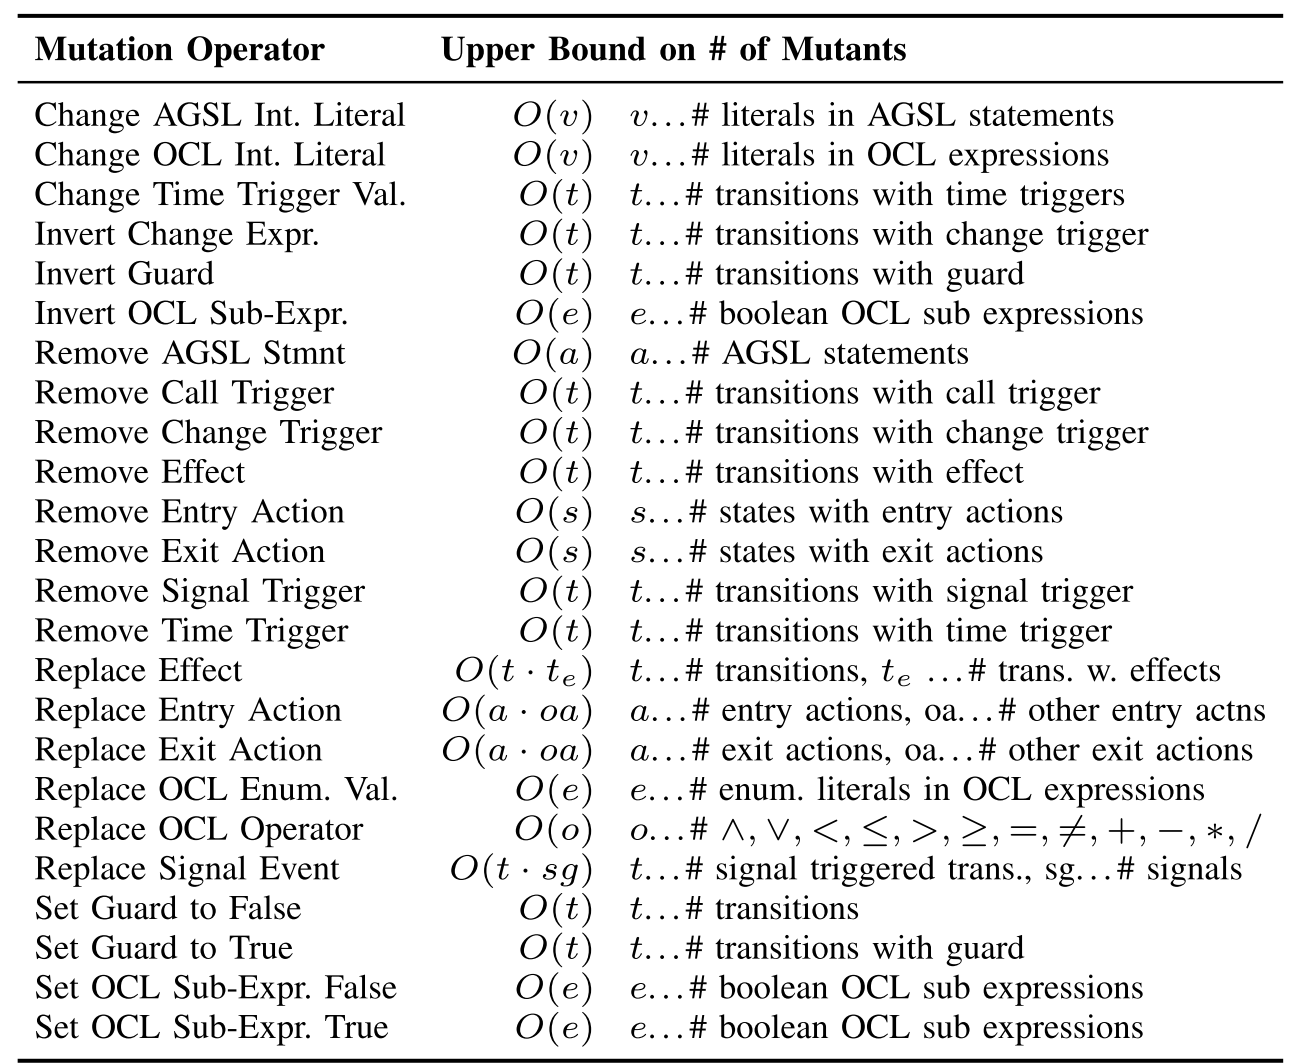
\includegraphics[width=0.6\textwidth]{images/aichernig2015}
%      \caption{Mutation operators introduced in \cite{Aichernig2015}.}
%\end{figure}
%
%%Test cases are generated by choosing a trace within the product graph starting from the initial state and ending at a fail state. Action systems usually describe non-deterministic behaviour, i.e. there can be multiple observable actions enabled at the same time and an implementation is allowed to choose among them. So, whenever there is a branch on observables in the product graph along the chosen trace to the fail state, this branch also is copied into the generated test case, yielding an adaptive test case.
%
%
%
%Model-based data mutation is not only applicable to UML models, in fact, Siavashi et al.~\cite{Siavashi2018} presented a model-based mutation testing approach for evaluating the authentication and authorization of web services in a multi-user context. The modeling of the web service and its security requirements are performed using an UPPAAL timed automata, the model is then mutated to create invalid behavior which is used for test generation to reveal faults in the SUT.
% 
%In model-based mutation testing (MBMT), the original test model is altered systematically by mutation operators creating multiple versions of a model, known as mutant models. The mutants can be used for automatic generation of invalid test inputs that are executed against the SUT. The goal in MBMT is to find whether any invalid tests can pass the testing, thus they can reveal unexpected behavior (i.e., a fault) in the SUT. Hence, MBMT can expose the mistakes that are caused by missing requirements or incorrect implementation.
%
%In the paper, authors model a web service, its users, and their authentication and authorization requirements. The model is then mutated to create invalid test inputs that target faults in the implementation of the web service. 
%
%Mutation testing extends the fault detection capabilities of MBT by exposing more vulnerabilities of systems. It changes a system's program or its specification, to create new versions of the system. 
%Mutation operators are rules that establish the mutants by altering the syntax of the program (or the specification). The generated tests exhibit altered inputs (including faulty inputs) and input sequences against the SUT. Hence the mutants allow testing of the SUT with invalid inputs. 
%
%The paper introduces eight mutation operators for timed automatas, five operators concern to action elements, and three to guard elements of the automata.
%
%\begin{table}[h!]
\begin{center}
\footnotesize
\begin{tabular}{|p{5cm}|p{10cm}|}
\hline
\textbf{Fault}&\textbf{Description}\\
\hline
Change Name of Actions (CN) & Replaces the name of an action with the name of other actions in the model. Thus, the expected sequence of the inputs to the implementation will be different..\\
Change Target of Actions (CT) & Changes the target location of an action to another location in the model. This operator breaks the flow of test inputs and violates the state of the model. Both input and output actions can be mutated by this operator.\\
Change Source of Actions (CS)& Changes the source location of an action to another location. Similar to CT, this operator mutates the sequence of input/outputs. \\
Remove Actions (RA)& randomly deletes one action at a time and creates a mutant. Omitting an action will manipulate the sequence of input/output actions.\\
Duplicate Actions (DA)& randomly copies an action in different parts of a model, thus alternates the sequence of inputs and outputs by repeating actions in unexpected states of the model.\\
Remove Guards (RG)& randomly selects an action and removes its guard. Actions that are mutated by RG will be always enabled.\\
Change Guards Logical Operators (CGL)& changes logical operators (i.e., ==, <=, >=, !=, < and >) in guards.\\
Change Guards Variables (CGV) & alters values of the variables that are used in guards and creates additional mutants that cannot be defined by other mutation operators\\
\hline
\end{tabular}
\end{center}
\caption{Fault Model from \cite{Siavashi2018}}
\label{table:faultModel:Siavashi}
\end{table}%

%
%%\textbf{MutRex: A Mutation-Based Generator of Fault Detecting Strings for Regular Expressions}
%
%Similarly, Arcaini et al.~\cite{Arcaini2017} proposed a model-fault-based approach for generating tests for regexes. The work is based on an automata representation of regexes that generates distinguishing strings exposing the faults introduced in mutated versions of a regex under test. The paper also introduces fault classes representing possible mistakes a user can make when writing a regex.
%
%The proposed tool, MutRex, first produces some mutants from a regex $r$ according to some fault classes representing common mistakes that are made when writing regexes; then, for each mutant $m$, it generates a string $s$ able to distinguish $m$ from $r$, i.e., a string that is evaluated differently in $r$ and $m$ (in terms of mutation testing, $s$ kills $m$). The set of generated strings is a test suite able to detect all the seeded faults.
%
%The authors identified three families of faults: \textit{single character faults}, \textit{character class faults} are respectively related to wrong uses of single characters and character classes, instead \textit{other faults} are related to wrong uses of the multiplicity and of the negation operator.
%
%\begin{table}[h]
%\caption{Mutation operators implemented by MutRex}
%\label{table:MutRex}
%\tiny
%\begin{tabular}{|p{3cm}|p{11cm}|}
%\hline
%\multicolumn{2}{|c|}{Single character faults}\\
%\hline
%Case Change CC & Regexes are case sensitive. However, a user could use them without being aware of this, or she could simply use the wrong case (either upper or lower). This operator mutates a regex r by changing the case of characters appearing in r: a mutant is created for each character of r not used in a character class, and a mutant is created for each character.\\
%Case Addition CA&This operator is similar to CC, but makes both lower and upper cases possible when only one of the two is used: for each character of the regex r not used in a character class it creates a mutant with the other case of the char added as alternative; for each character class, instead, the mutant adds as alternative a new character class having the extremes of the interval in the other case.\\
%Metachar to Char M2C& In a regex, some characters can be interpreted as metachars or chars depending on the context, and there is no mandatory special way to identify metachars. For example, character '-' is interpreted as a metachar only in character classes, otherwise it matches the normal dash character. A user may want to use a char c, but she could wrongly use c as metachar. This operator transforms a regex r containing a char c interpreted as a metachar in a regex r' in which c is interpreted as a char. Note that the way to mutate r depends on the metachar c: for example, M2C applied to '-' removes the character class where '-' is used.\\
%Char To Metachar C2M & In other cases, instead, the designer wants to use a metachar c, but, because of the context, c is interpreted as a simple char. This operator transforms a regex r containing a c interpreted as a char in a regex r' in which c is interpreted as a metachar. Similarly to M2C, the way to mutate r depends on the metachar c.\\
%\hline
%\multicolumn{2}{|c|}{Character class faults}\\
%\hline
%Character Class Creation CCC& Character classes are delimited by square brackets []. A user may want to use a character class and forgets (or ignores) the parentheses. Given a regex $r = c_{1}-c_{2}$, the operator mutates $r$ in $r'= [c_{1} - c_{2}] $.\\
%Character Class Addition CCA&The user could have forgotten a given interval in a set of character classes. Given a regex $r = [cc_1 ... cc_n]$, the operator creates a mutant $r' = [cc_1 ... cc_n cc_{new} ]$ for each $cc_new$ not present in r; $cc_{new}$ can be a-z, A-Z,or 0-9.\\
%Range Modification RM&The user could have specified the operator produces a mutant in which $c_1$ or $c_2$ is increased a too tight or too broad interval. Given a regex $r = [c_1 - c_2]$, or decreased (if it is still a valid char). \\
%Character Class Restriction CCR& The user could have written a regex that is too permissive since it accepts characters that should not. Given a regex $r =[cc_1 ... cc_n]$, the operator creates a mutant $r' = [cc_1 ... cc_{i-1}cc{i+1} ... cc_n]$ for each $cc_i$ (i.e., it removes an interval from the character class).\\
%Prefix Addition PA& Sometimes all the characters of a string $s$ satisfy some constraints, except for the first character in $s$ that must satisfy additional constraints; for example, identifiers in most programming languages cannot start with a number. This mutation operator, given a repeat expression regex $r =[cc_1, ..., cc_n]m$ (being $m$ the multiplicity), introduces a prefix that is one of the different character classes $cc_1, ..., cc_n$ used in $r$. The obtained mutants are as follows: $[cc_1][cc_1, ..., cc_n]m, [cc_2][cc_1, ..., cc_n]m, ..., [cc_n][cc_1, ..., cc_n]m$.\\
%Character Class Negation CCN& Regex [ˆ$cc_1 ... cc_n]$ matches any character that is not listed in the character classes $cc_1, ..., cc_n$. The designer could have forgotten the ˆ symbol and written $[cc_1 ... cc_n]$. CCN introduces symbol ˆ it creates a mutant in which all the character classes are excluded (i.e, [ˆ$cc_1 ... cc_n$]), and a mutant for each character class $cc_i$ in which only $cc_i$ is excluded (i.e, $[cc1] | ...| [$ˆ$cc_i] | ...| [cc_n])$.\\
%
%Negated Character Class to Optional NCCO& Another common error regarding the use of a negated character class [ˆcc] is that it requires 'to match a character that is not listed' and not 'to not match what is listed'. Therefore, a negated character class still requires to match a character. A user could misunderstand the semantics of the operator, thinking that it simply excludes the character; in some cases, for example at the end a word, she could be interested in accepting also no character. Operator NCCO makes ˆ optional, i.e., it mutates [ˆcc]in[ˆcc]?\\
%\hline
%\multicolumn{2}{|c|}{
%Other faults}\\
%\hline
%Negation Addition NA&In a regex $r = r_1r_2 ...r_n$, the user could forget a negation ˆ. The operator creates a mutant adding a negation wherever possible in $r$, i.e., ˆ$r_1r_2 ...rn, r_1$ˆ$r_2r_n, ..., r1r2 ... $ˆ$r_n$. \\
%Quantifier Change QC&The user could have used the wrong cardinality. The operator mutates each simple repeat quantifier in another simple quantifier; moreover, for each user-defined quantifier, it creates a mutant in which $n$ (or $m$) is increased and a mutant in which it is decreased.
%Example\\
%\hline
%\end{tabular}
%\end{table}
%
%
%A mutant $m$ of a regex $r$ can modify the accepted language in four ways: 
%\begin{itemize}
%  \item Arbitrary edit: some words are added to the language and other words are removed.
%  \item Generalization: some words are added to the language and no word is removed.
%  \item Specialization: some words are removed from the language and no word is added.
%  \item Equivalent: the mutant is equivalent and so the two languages are the same.
%\end{itemize}
%
%
%%\textbf{Combinatorial mutation approach to web service vulnerability testing based on SOAP message mutations}
%
%In a different context, Li et al.~\cite{Li2012} proposed a model-based combinatorial mutation approach based on SOAP messages for Web service vulnerability testing.
%The technique presented in the paper consists of (1) analyzing the web service methods and identify all the associated web service methods. (2) Invoke different sets of mutation operators according to the perturbation policy on the SOAP messages (XML documents) by parsing the WSDL files, and then (3) call the appropriate combinatorial testing approach to generate combinatorial test cases.
%
%The XML model-based approach presents the following two perturbation policies: data value and interaction perturbations. Both perturbation policies directly act on the SOAP messages. The former one modifies values in SOAP messages according to their data types while the latter one may consider the data values and data relationships. Part of the mutation operators bear double effects of data value and interaction perturbations.
%
%The following mutation operators were introduced:
%
%\begin{figure}[h]
%  \centering
%    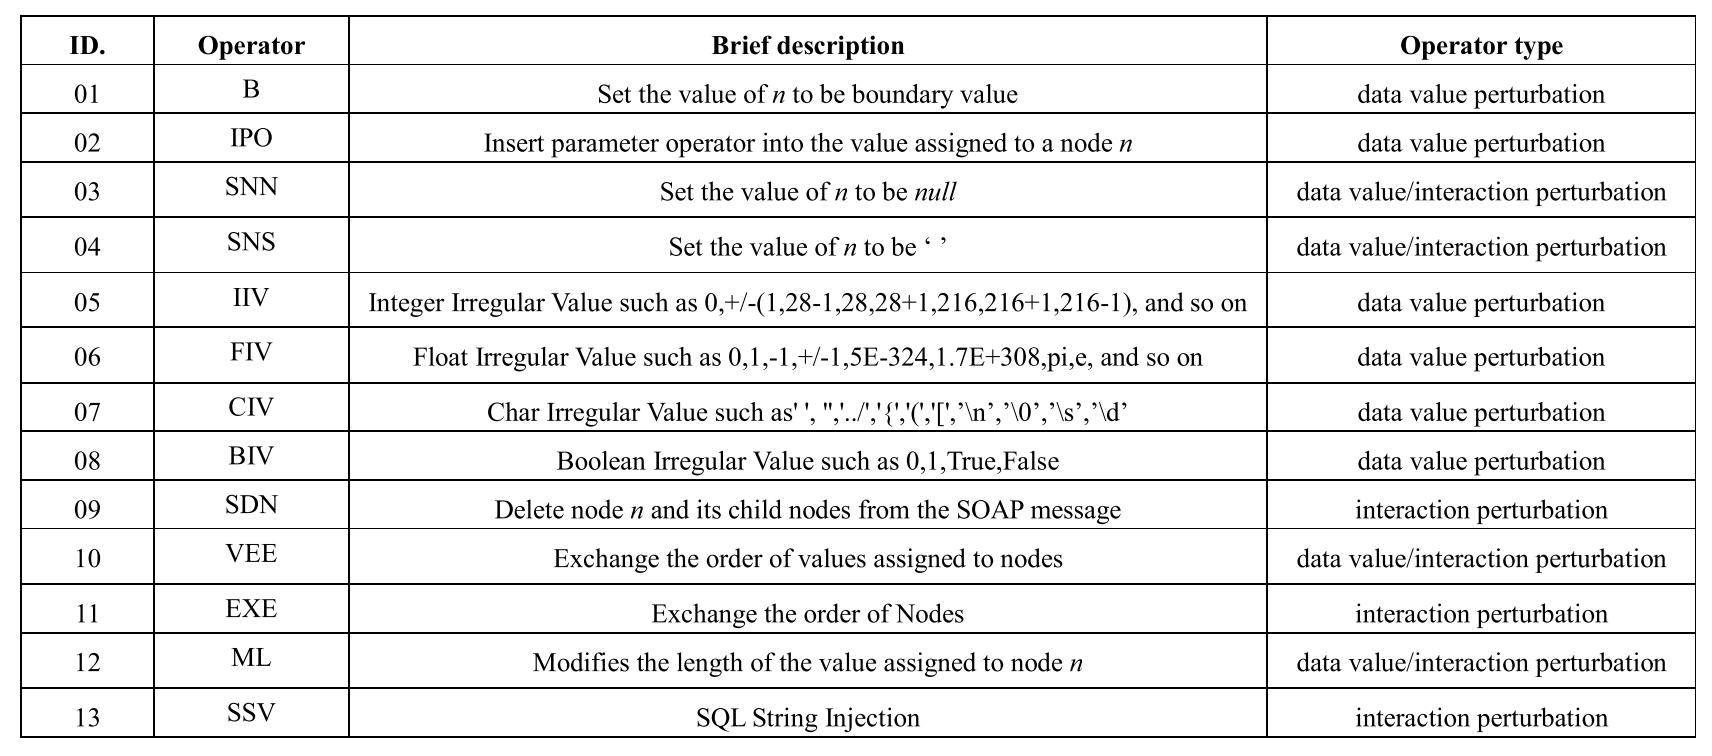
\includegraphics[width=\textwidth]{images/li2012}
%      \caption{Combinatorial mutation approach to web service vulnerability testing based on SOAP message mutations \cite{Li2012}}
%\end{figure}
%
%%\textbf{Worst-input mutation approach to web services vulnerability testing based on SOAP messages}
%
%Similarly, Chen et al.~\cite{Chen2014} introduced a model-based mutation approach for testing web service vulnerability of SOAP messages. 
%
%The method involves partitioning the input domain into sub-domains according to the number and type of SOAP message parameters in the TCFN (test case farthest neighbor) and then selecting the candidate test case whose distance is the farthest from all executed test cases and applying it to test the Web service.
%
%Web service vulnerability refers to flaws in the service that threaten the security of the computer system, for example, memory leaks, buffer overflows, and cross-boundary access (where memory variables access areas outside their defined scope)
%
%SOAP is a message protocol based on an XML document, which forms the basis of the mutation object. The paper introduces 15 mutation operators for SOAP parameters types combined with Web service features.
%
%\begin{figure}[h]
%  \centering
%    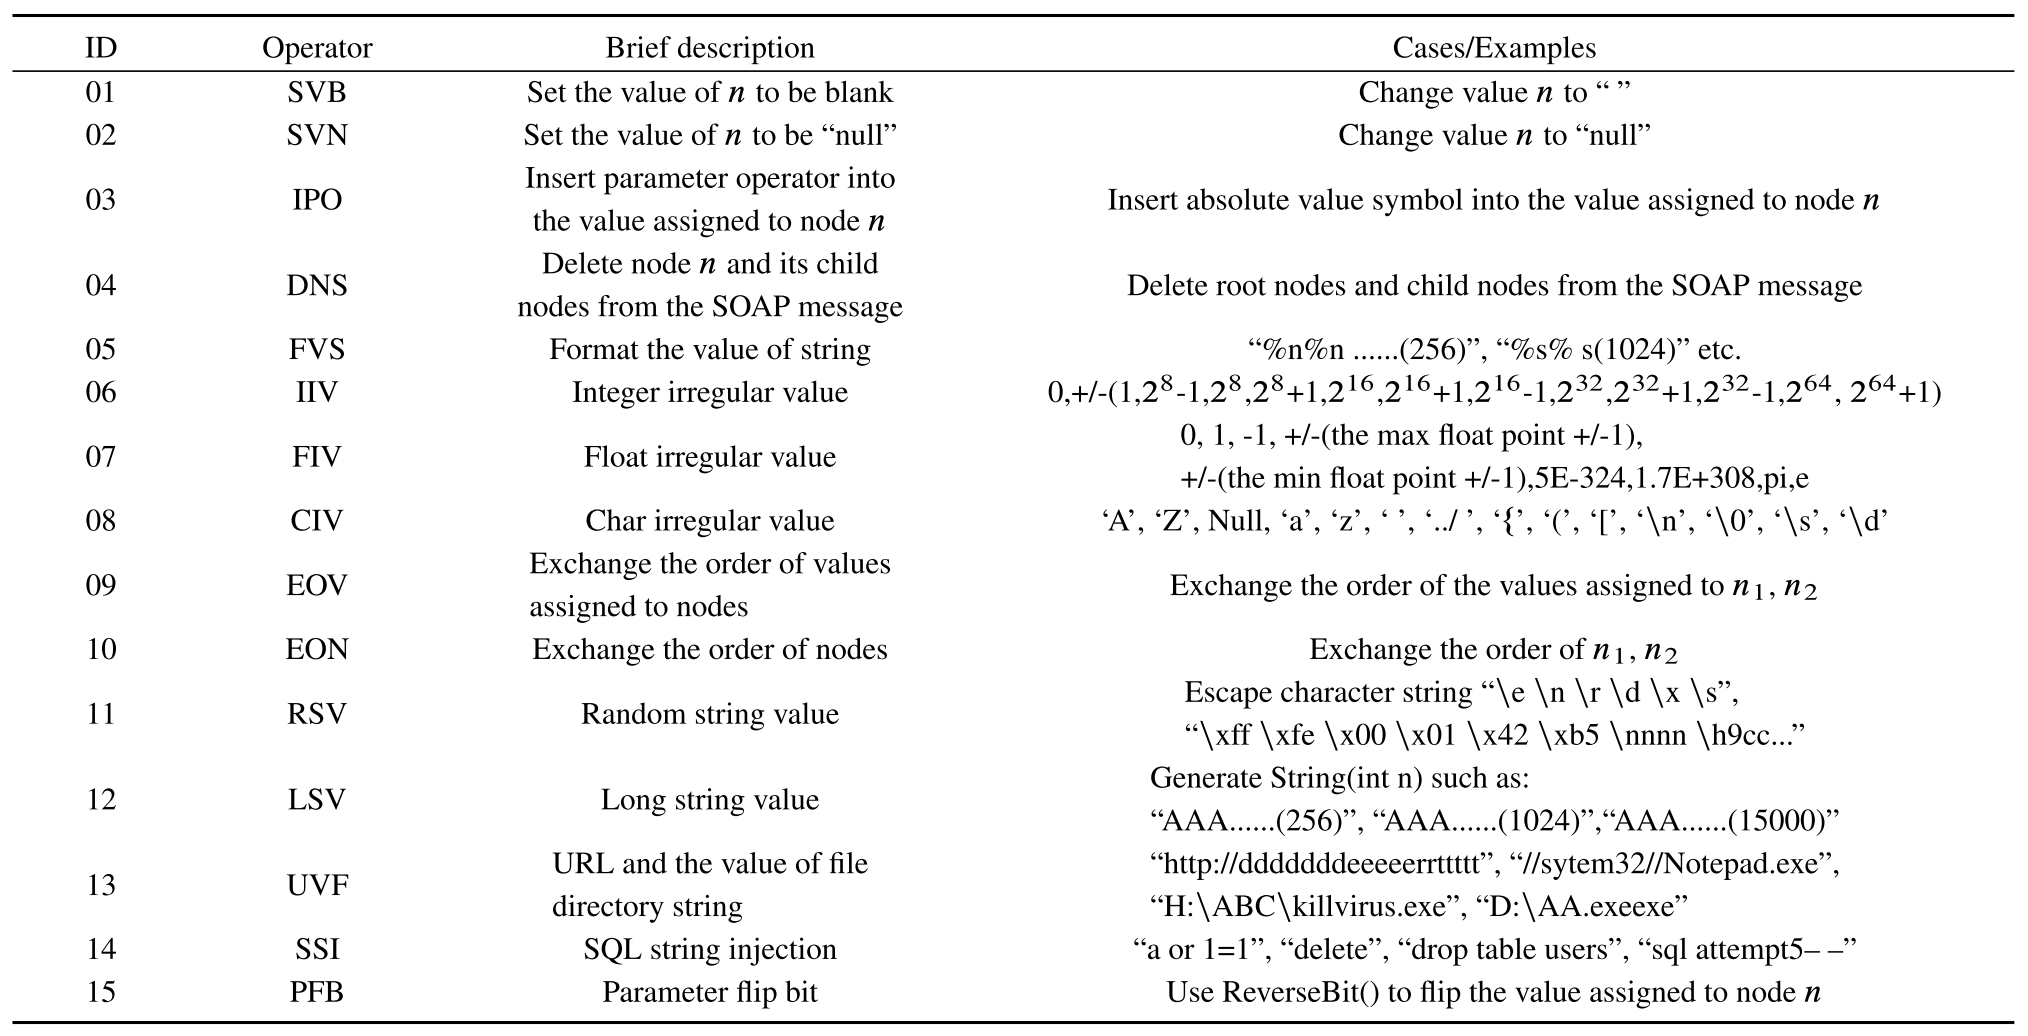
\includegraphics[width=0.8\textwidth]{images/chen2014}
%      \caption{SOAP messages mutation operators.}
%\end{figure}
%
%
%\subsubsection{Search-based data mutation}
%
%Search-based data mutation relies on an evolutionary algorithm to perform model-based data mutation and optimize multiple objectives:  
%cover all the classes of the data-model, cover all the possible faults of the fault model, cover all the clauses of the input/output constraints,
%maximise code coverage~\cite{di2015evolutionary}.
%The coverage of each objective is encoded by means of boolean arrays; this information is used to select a minimal set of inputs that maximize the coverage of the different objectives.
%At every iteration, the evolutionary algorithm keeps only inputs that contribute to increase the coverage of at least one of the objectives (e.g., inputs that cover one instruction not covered by other inputs).
%
%An additional source of information concerning the adoption of fuzzing and grammar-based approaches to perform test input generation is the \emph{Fuzzing Book}~\cite{fuzzingbook2019:GrammarFuzzer}.
%
%
%\subsection{Automated Detection of Equivalent and Redundant Mutants}
%\label{sec:dataequivalent}
%
%Data-driven mutation operators may lead to the generation of both equivalent and redundant mutants.
%In the data-driven context, equivalent mutants consist of modified data (i.e., data altered by means of mutation operators) that do not lead to any noticeable difference in the output of the SUT with respect to the original version of the data.
%Please note that an equivalent mutant differs in content from the original data (i.e., the data chunk has been altered).
%The possible reasons why a mutant may not lead to noticeable differences in the output of the SUT are three. First, changes may go unnoticed because they alter portions of the data that is not read by the SUT. This includes cases in which mutations alter the structure of the input data in such a way that the resulting mutated data is different from the original but still respect the data format. This might happen, for example, when a mutation operator swaps the CDATA section of an XML file and the SUT ignores CDATA content. Second, mutations may alter some of the outputs of the SUT but the test suite oracles ignore that portion of the output. This might happen in a data acquisition system that copies the data payload of network packets in a database; in such a context, a data mutation that alters the message and update the packet checksum might go unnoticed because the SUT would simply copy the message content to the database and the test suite may simply check if the database contains a new message. Third, mutations may alter valid existing data but produce data that is still valid. This often reflect a poor choice of mutation operators; indeed, the selected mutation operators should guarantee to introduce a fault in the data exchanged by the system.
%
%
%Redundant mutants cause the same failures in the test suite. Two are the reasons for redundant mutants. First, the mutations alter different instances of a same data structure in the same way (e.g., delete a message in a sequence). Second, the mutations alter data chunks that are ignored by the oracles of the test suite.
%
%Concrete examples of equivalent and redundant mutants are provided in Figure~\ref{fig:data:quivalent}. In Figure~\ref{fig:data:quivalent}, \emph{Mutation 2} leads to an equivalent mutant since it generates a timestamp that is just one millisecond in the past, which is legal for the system under test. The value 2 for a timestamp, instead, leads to a failure because is considered too much in the past (see \emph{Mutation 1}). To address this problem, engineers should have configured the timestamp field to be mutated by a boundary condition operator (which generates values out of valid range) instead of a bit flipping operator. \emph{Mutation 3}  and \emph{Mutation 4}, instead, are redundant because they both generate a timestamp in the future (under the assumption that \emph{1584889773} captures the current time).
%
%\begin{figure}[h]
%  \centering
%    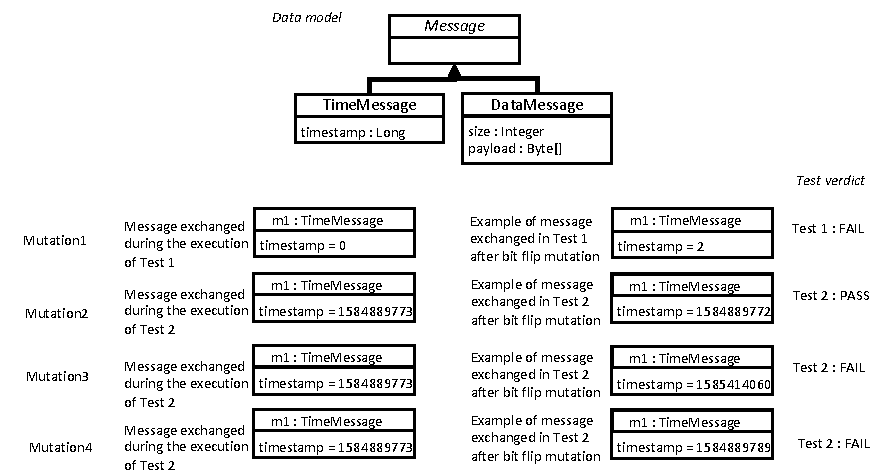
\includegraphics{images/DataDrivenEquivalent}
%      \caption{Examples of data-driven mutations leading to equivalent and redundant mutants.}
%      \label{fig:data:quivalent}
%\end{figure}
%
%Literature lacks approaches to directly target equivalent and redundant mutants. However, some of the solutions implemented in existing data mutation approaches might limit the presence of equivalent and redundant mutants. We observe three main solutions: (1) driving mutations by means of code-coverage, (2) driving mutations by means of coverage of model structure, and (3) use of model-based oracles.
%
%Code-coverage-driven mutations are the ones implemented by many automated fuzzers such as 
%MoWF~\cite{pham2016model} and AFL~\cite{gutmann2016fuzzing}.
%MoWF aims to generate mutated data that triggers the execution of specific code locations. This is done by combining symbolic execution and meta-heuristic search.
%Since each mutated input triggers a different code location, MoWF, in principle, should always lead to mutated inputs that make the software behave differently than with the original input or with other data mutants. However, it does not ensure that the changes in the internal behaviour of the software are reflected in one of its observable outputs.
%Similarly to MoWF, AFL generates inputs that trigger different code locations. The main difference is that it does not target only specific code locations but it aims to exercise all the branches of the program. 
%Similarly to MoWF, AFL does not guarantee that changes in the internal behaviour of the software are reflected in one of its observable outputs.
%Similarly to AFL, any approach relying on meta-heuristic search that include coverage objectives in the fitness function (e.g.,~\cite{di2015evolutionary}) can limit the presence of equivalent and redundant mutants.
%
%
%The coverage of the model structure enables the generation of mutations targeting different portions of a given data model.
%For example, \emph{pFuzzer} generates valid inputs that cover diverse sets of lexical and syntactical features.
%Other approaches~\cite{di2015generating} generate mutants that target different elements of the data structure.
%By targeting different elements of the data, the generated mutants are unlikely to be redundant or equivalent. However, they do not ensure that such differences are reflected in the SUT observable outputs.
%
%
%Model-based oracles, such as OCL constraints capturing expected outputs (e.g., error messages expected in the presence of a specific change of the data) enable the generation of mutants that are not equivalent and not redundant. For example, by ensuring that each mutant affects a model element referenced in a different OCL constraint and that the constraint is evaluated to true, model-based mutation approaches can guarantee that the data mutations lead to observable changes in the SUT output~\cite{di2015generating}.
%
%
%\newcommand{\ONMO}{\mathit{overall}\ \# \mathit{of}\ \mathit{mutation} \ \mathit{operators}}
%\newcommand{\NMOA}{\# \mathit{of}\ \mathit{mutation} \ \mathit{operators} \ \mathit{applied}}
%
%
%\subsection{Analysis of Mutation Testing Results and Mutation Score Calculation}
%\label{sec:data:mutationscore}
%
%In the data-driven mutation testing process, the outcome of the activity \emph{Analyze Results} (see Figure~\ref{fig:data:process}) is a mutation score that is based on
%the percentage of mutants being killed and the percentage of mutation operators applied. 
%The former enables data-driven mutation to achieve objective O1 in Section~\ref{sec:dataProcess}, the latter objective O2. 
%The mutation score can be computed as a weighted average of the percentage of mutants being killed and the percentage of mutation operators applied, according to the following formula
%
%\begin{equation}
%Score=w_{O1} \frac{\# \ \mathit{of}\ \mathit{killed} \ \mathit{mutants}}{\mathit{overall} \# \mathit{of}\ \mathit{mutants}} + w_{O2} \frac{\# \mathit{of}\ \mathit{mutation} \ \mathit{operators} \ \mathit{applied}}{\mathit{overall} \# \mathit{of}\ \mathit{mutation} \ \mathit{operators}}
%\label{f:mutation:score}
%\end{equation}
%
%Where $w_{O1}$ and $w_{O2}$ capture the importance of the objectives O1 and O2, respectively. We assume $w_{O1}$ + $w_{O2} = 1$. In case objective $w_{O1}$ and $w_{O2}$ have the same importance, they should be set to $0.5$. In the case of safety-critical systems, the mutation score should be equal to 1.
%
%In formula \ref{f:mutation:score}, the $\mathit{overall}\ \# \mathit{of}\ \mathit{mutants}$ corresponds to the number of test executions in which at least one data object have been altered through mutation. We refer to such test executions as \emph{mutated test executions}.
%The $\# \ \mathit{of}\ \mathit{killed} \ \mathit{mutants}$ corresponds to the number of \emph{mutated test executions} that either failed or during which a redundancy mechanisms has been activated to handle the mutated data.
%
%The $\ONMO$ corresponds with the number of different mutations that can be applied to the data, according to the data model. It depends on the strategy adopted to select the items to be mutated.
%% and may vary based on the strategy adopted to perform data mutation.
%For approaches relying on \textbf{UML models}, one possibility is to follow the approach of Di Nardo et al.~\cite{di2015generating}, which consists of mutating every model element (e.g., class or class attribute in the class diagram capturing the data model) with every mutation operator that is applicable to the specific model element, according to the fault model captured in the class diagram (see Section~\ref{sec:data_operators}).
%The $\ONMO$ (ONMO) could be thus computed as the sum of the number of applicable mutation operators for ever every model element.
%The $\NMOA$, (NMOA) consequently, should capture the number of mutations that were performed. In the approach of Di Nardo et al.~\cite{di2015generating}, NMOA corresponds to the number of model elements for which at least one instance had been mutated. 
%
%For the computation of ONMO and NMOA, a strategy similar to the one presented by Di Nardo et al. can be used also in the case of approaches relying on \textbf{grammars} or \textbf{block models}. Indeed, also for these two types of approaches, data mutation is performed by means of a set of mutation operators that are applied in the presence of specific data types. 
%These data types correspond to the production rules of the grammar or the blocks defined in the block model. 
%Approaches that do \textbf{not require an input model} typically work at the bit/byte level. In these cases, ONMO might be calculated as the number of available operators, or
%as the number of bit/bytes in the inputs multiplied by the number of applicable mutation operators.
%
%
%Moreover, data njection has been usually used to asses the robustenss of software here we apply to assess the test suite with respct to interoperability faults.
%%this is the first work relying on data fault injection procedures to perform mutation analysis.

% !TEX root = MAIN.tex

\clearpage
\section{Code-driven Mutation Testing}
\label{sec:back:testGeneration}

This section describes the approaches that can be adopted to automatically generate test cases that kill mutants.
To kill a mutant we need test cases that (1) reach the mutation point (i.e., execute the mutated code), (2) cause 
corruptions
in the program state right after the mutated code,
and (3) manifest these corruptions into the program output 
(e.g., by producing an erroneous value in a state variable verified by a test assertion) 
thus leading to a failure~\cite{papadakis2019mutation}. These conditions are also known as the \INDEX{killing conditions} of a mutant.

In the literature, there exist two groups of approaches for 
generating test cases that kill mutants:
approaches based on constraint-programming, and approaches based on evolutionary computation. Below we introduces these two stream of approaches after introducing two well-known solutions for test generation driven by structural coverage, which are the basis for mutation testing solutions based on constraint programming.

\subsection{Test Generation driven by program structure}
\label{sec:back:generation:structure}
Two alternative state-of-the-art solutions to generate test inputs that maximize structural coverage are CBMC, a bounded model checker, and KLEE~\cite{cadar2008klee}, a symbolic execution engine. They are detailed below.

%\subsubsection{CBMC}
%\label{subsec:cbmc}

\INDEX{CBMC} is an approach that implements \INDEX{Bounded Model Checking}~\cite{BiereCCZ:TACAS99,SeryFS:ATVA12} (BMC), an approach for purely static software verification.
The idea in BMC is to represent the software together with the
properties to be verified as an instance of the propositional
satisfiability problem (SAT).  Such a representation captures the
software behavior exactly, assuming that all the loop bodies in the
software are repeated at most a fixed number of times.
This approach has several advantages: the logical formulation is usually
very compact compared to traditional model checking, where verification
is reduced to a reachability problem in a graph representing the program
state space;
%
there are several high-performance SAT
solvers~\cite{MarquesSilva:IEEETRAN99,EenS:SAT2003} that can be used for
solving the instances;
%
and the satisfying assignments of an instance can be directly translated
to meaningful counterexamples for correctness in the form of
fault-inducing executions.
%
Furthermore, it is widely recognized that BMC based approaches are particularly good
at quickly finding short counterexamples when they exist.

%A {\em bounded model checker} takes as input a program $\prog$, a bound $k$
%for loop unrolling, and a set $S$ of properties to be verified against
%$\prog$, and returns for each property ${l}$ in $S$, expressed as a propositional statement over variables of $\prog$ at a location $l$, either \vspace{-0.2cm}
%\begin{itemize}
%    \item \emph{verified}, if the executions of $\prog$  satisfy $\prop{l}$;\vspace{-0.25cm}
%    \item \emph{unreachable}, if no execution of $\prog$ reaches $l$;\vspace{-0.25cm}
%    \item \emph{false}, if there is an execution of $\prog$
%    where the property $l$ is broken; and\vspace{-0.25cm}
%    \item \emph{unknown}, if the checker is unable, due to
%    memory or time limits, to determine whether ${l}$ holds,\vspace{-0.2cm}
%\end{itemize}
%under the assumption that no loop body in the program is repeated more
%than $k$ times.
%
%The approach is naturally a compromise between practicality and
%completeness.
%As the SAT problem is \INDEX{NP-complete}, determining whether $\prop{l}$ holds
%requires in the worst case exponential time with respect to the size of
%the SAT instance for all known algorithms.
%%
%Furthermore, the instances can in some cases grow very large since many
%operations, such as multiplication, have quadratic encodings in SAT and,
%for example, the instance grows exponentially in number of nested loops.
%%
%
%Due to numerous optimizations BMC can nevertheless solve many practical
%problems in reasonable time and memory limits.
%%
%For example, the size of the resulting SAT instance can be dramatically
%reduced by slicing off parts of the program that do not affect the
%validity of the property being checked, and
%%
%extremely efficient SAT solver implementations which learn the instance
%structure and use adaptive heuristics~\cite{MahajanFM:SAT04} rarely
%suffer from the exponential worst-case behavior in problems emerging
%from applications.
%%
%The fact that bounded model checkers only prove correctness of
%properties for executions not exceeding the bound $k$ is also beneficial
%in many ways for detecting regressions.  In addition to obvious
%performance benefits our experiments show that in most cases even a single
%loop iteration is sufficient to indicate a regression between two
%versions, and a small bound guarantees in a natural way that the
%reported counterexamples are short.

%\subsubsection{KLEE}

\INDEX{KLEE}~\cite{cadar2008klee} is an open source tool that implements {\INDEX{Concolic Execution}}, a technique that performs \INDEX{symbolic execution} along a concrete execution path. KLEE was designed to automatically generate test cases that achieve high code coverage. The tool is implemented as a modified LLVM virtual machine that targets LLVM bytecode programs.
KLEE also provides a symbolic POSIX library that enable analysis of programs that uses the system's environment. For example, KLEE can be executed with the flag \texttt{-sym-stdin N} which will make stdin symbolic with size \texttt{N}.  

In FAQAS, we rely on KLEE to automatically produce the inputs that make the mutated version of the program generate a different output than the original version.



\subsection{Test Generation based on Constraint Programming}
\label{sec:testGen:CP}

Techniques based on constraint programming use some form of automated reasoning (e.g., Propositional Satisfiability or Constraint Solving~\cite{SATandCPsurvey:2006}) to derive data that satisfy all the conditions necessary to kill a mutant~\cite{offutt1997automatically}.Existing approaches, differ for the strategy adopted to automatically generate these constraints from the program under test.

Offutt et al.~\cite{offutt1997automatically}, for example, automatically derive such constraints from the program by extracting the predicate expressions on the program's control flow graph.
Then, such constraints are encoded to form a constraint system. In their approach, they propose three strategies for identifying infeasible constraint systems, the contradictions to such systems are the new test cases for the program under analysis.

% !TEX root =  ../MutationTestingSurvey.tex

\begin{lstlisting}[style=CStyle, caption=midval function returns the mid value between three integers., label=midval, mathescape=true]
int midval (int x, int y, int z) {
	int midval;

	midval = z;
	if (y < z) {
		if (x < y) {
			midval = y;
		}
		else if (x < z) 
 $\Delta$ else if (x <= z) {
			midval = x;	
		}
	}
	else 
		if (x > y) {
			midval = y;
		} else if (x > z) {
			midval = x;
		}
	return midval;
}
\end{lstlisting}

In the following, we introduce an example of the application of Offutt's~\cite{offutt1997automatically} approach by using the \texttt{midval} function presented in Listing~\ref{midval}. This function has a mutation on line 9, which has been mutated into line 10. According to their approach, the three killing conditions would be the following:

\begin{itemize}
	\item Reachability $C_R: (y < z) \wedge (x \geq y)$
	\item Necessity $C_N: (x < z) \neq (x \leq z)$
	\item Sufficiency $C_S:$ Output(P) $\neq$ Output(M)
\end{itemize}

$C_R$ defines the condition required to reach the mutated statement, in this case the conjunction between the predicate of the first if condition and the negation of the second if condition. $C_N$ defines the condition required to assure a different program state between the original and mutated version of the program right after the mutation point. Finally, $C_S$ defines the condition necessary to demonstrate that both the original and the mutated program returns different values.

Holling et al.~\cite{holling2016nequivack} proposed to use a \INDEX{symbolic execution} approach to identify new test cases. Their idea is to first execute symbolically both the original and the mutated function, then to check if their return values are equivalent or not. 
Symbolic execution determines what inputs cause each part of a function to be covered during execution. To symbolically execute a function, it is necessary to replace the original inputs (i.e., concrete values) with symbolic ones. The \INDEX{symbolic values} represent a set of possible concrete values that lead to a certain program path (i.e., path condition). 


Holling's approach~\cite{holling2016nequivack} to automatically identify equivalent mutants relies on the observation that 
two mutants are equivalent when there are no concrete values making the mutated function produce an output that is different from the one of the original function.
If a value that makes the two functions generate distinct results can be found, the mutant is non-equivalent.
To automate the generation of inputs, Holling et al. rely on KLEE~\cite{cadar2008klee}.

We introduce an example of Holling's approach in Listing~\ref{function}. The top part of Listing~\ref{function} shows the function \texttt{isPositive}, which checks if an integer number is positive or not. The bottom part of Listing~\ref{function} presents the mutated version of \texttt{isPositive}, where the relational operator $\geq$ has been replaced by the operator $>$.
To automate the generation of inputs using KLEE, all the parameters need to be treated as symbolic values.
%F: "the \texttt{isPositive} parameter \texttt{num}" it's impossible to understand what is the parameter and who owns the parameter
%In Holling's approach, first, the \texttt{isPositive} parameter \texttt{num} needs to be treated as symbolic value, which is done by the function \texttt{make\_symbolic} (see Listing~\ref{example}) which converts concrete variables to symbolic by considering its memory address and size. 
This is achieved by function \texttt{make\_symbolic} (see Listing~\ref{example}) which converts concrete variables to symbolic ones by considering their memory address and size. 
%F: please fix
In Listing~\ref{example}, the parameter \texttt{numSymbolic} is made symbolic in Line 3. Then, the original and mutated functions are called using the symbolic arguments in Lines 5 and 6.
%Finally, the \texttt{assert} function of line 8 verifies if the integer return values of both functions are equal or not.
Finally, we need to introduce an assertion that makes the symbolic execution engine \EMPH{look for inputs that make the output of the two functions different}. 
In Listing~\ref{example}, this is achieved with an assertion that verifies that the return values of the two functions the same (see Line 8). 
Despite being counter-intuitive, this approach is effective because symbolic execution engines aim to identify inputs that falsify the assertions in the program. 
When the equality is falsified, then the two functions can produce a different output for a same input.
The input that falsifies the equality can thus be used to improve the test suite enabling it to kill the mutant.
In the example of Listing~\ref{example}, KLEE will indicate that the return values of the original and mutated function differ when \texttt{num} is equal to zero.
A new test case exercising function \texttt{isPositive} with \texttt{num=0} should thus be added to the test suite in order to kill the mutant.

\begin{lstlisting}[style=CStyle, caption=isPositive and MUT\_isPositive functions, label=function]
int isPositive(int num){
	if (num >= 0){
		return 1;
	} else {
		return 0;
	}
}

int MUT_isPositive(int num){
	if (num > 0){
		return 1;
	} else {
		return 0;
	}
}

\end{lstlisting}

\begin{lstlisting}[style=CStyle, caption=Holling's approach for test case generation., label=example]
void test () { 
	int numSymbolic; 
	make_symbolic(&numSymbolic, sizeof(numSymbolic), "numSymbolic"); 
 	
 	int original_ret = isPositive(numSymbolic); 
	int transformed_ret = MUT_isPositive(numSymbolic); 
 
	assert(original_ret == transformed_ret); 
}
\end{lstlisting}

Similarly to Holling's approach, Riener et al.~\cite{riener2011test} proposed to use \INDEX{bounded model checking} techniques to search for these counter examples.
In their bounded model checking approach, the original program and the mutant are unrolled with respect to a certain maximum bound. In program unrolling, loops are re-written as a repeated sequence of similar independent statements. Then, both unrolled programs are encoded into a logic formula over the same input variables. To ensure that the mutation affects the output of the mutant, a propagation condition is encoded and added to the previous logic formula, the condition asserts that there exist at least one pair of different outputs under the assumption of equal inputs. In the last step, the formula is processed by a SMT-solver, if the solver finds a satisfying assignment, the inputs of the formula are translated into a new test case for the current program under analysis.

%Compared to symbolic execution, one advantage of bounded model checking is that it does not require to execute the whole program but may focus on the mutated functions only.

%To reduce the time required by the symbolic execution process, which needs to be performed against all the mutants of the software, Papadakis et al.~\cite{papadakis2011automatically, papadakis2010towards} propose to combine symbolic execution techniques and \INDEX{mutant schemata} to automatically generate test cases targeting the killing conditions induced by the different mutants embedded into the same executable. The approach targets \INDEX{weak mutation} testing and may not generalize to strong mutation testing. Indeed, ensuring the sufficiency property (i.e., verify that changes are propagated to outputs) for multiple mutants might lead to scalability issues not addressed by the proposed approach.





\INDEX{SEMu}~\cite{chekam2021killing} is a recent mutantion testing  framework based on dynamic symbolic execution that has been built on top of the KLEE Symbolic Virtual Machine~\cite{cadar2008klee}.
SEMu uses a form of \INDEX{differential symbolic execution}~\cite{person2008differential} to generate test inputs that kill mutants. The approach consists of modeling the mutant killing problem as a symbolic execution search in a scalable and cost-effective way. 
The SEMu framework is the building block of 
%act as a baseline for 
the test generation tool developed in FAQAS (i.e., \INDEX{SEMuS}). Different from the approaches presented above, SEMu can generate test inputs that kill mutants without the need of human intervention (e.g., to ad assertions); however, it targets only bash programs, it cannot generate unit test cases, for example.

%To kill a mutant, we need test cases that capture the three killing conditions of a mutant~\cite{offutt1997automatically}: 
%\begin{itemize}
%	\item \INDEX{reachability}: the test case should execute the mutated statement
%	\item \INDEX{necessity}: the test case should cause an incorrect intermediate state, if it reaches the mutated statement
%	\item \INDEX{sufficiency}: the final state of the mutated program should differ from the one of the original program
%\end{itemize}

%\DONE{the concept of "mutation point is not clear"; you do not clarify that the two versions are compiled in the same executable}

In SEMu, the multiple program versions (i.e., the original and the mutated programs) are compiled within the same executable. 
Because mutants differ only slightly from the original program (minor syntactic differences), the technique performs one symbolic execution search for the unchanged source code, and then it forks the symbolic execution search every time it reaches a mutated statement.

The technique follows both the mutated and the original execution and compares the state (i.e., the value of the variables) at each step of the execution.
More precisely,  every time the execution reaches the statement after the mutation, the technique triggers the generation of test inputs for the forked and the original programs by comparing their symbolic states. To generate test inputs that kill the mutant, the technique encodes the three killings conditions, obtained from the symbolic execution search, into a single formula (the $kill$ formula) to be passed to a constraint solver.

%\begin{figure}[tb]
%\begin{center}
%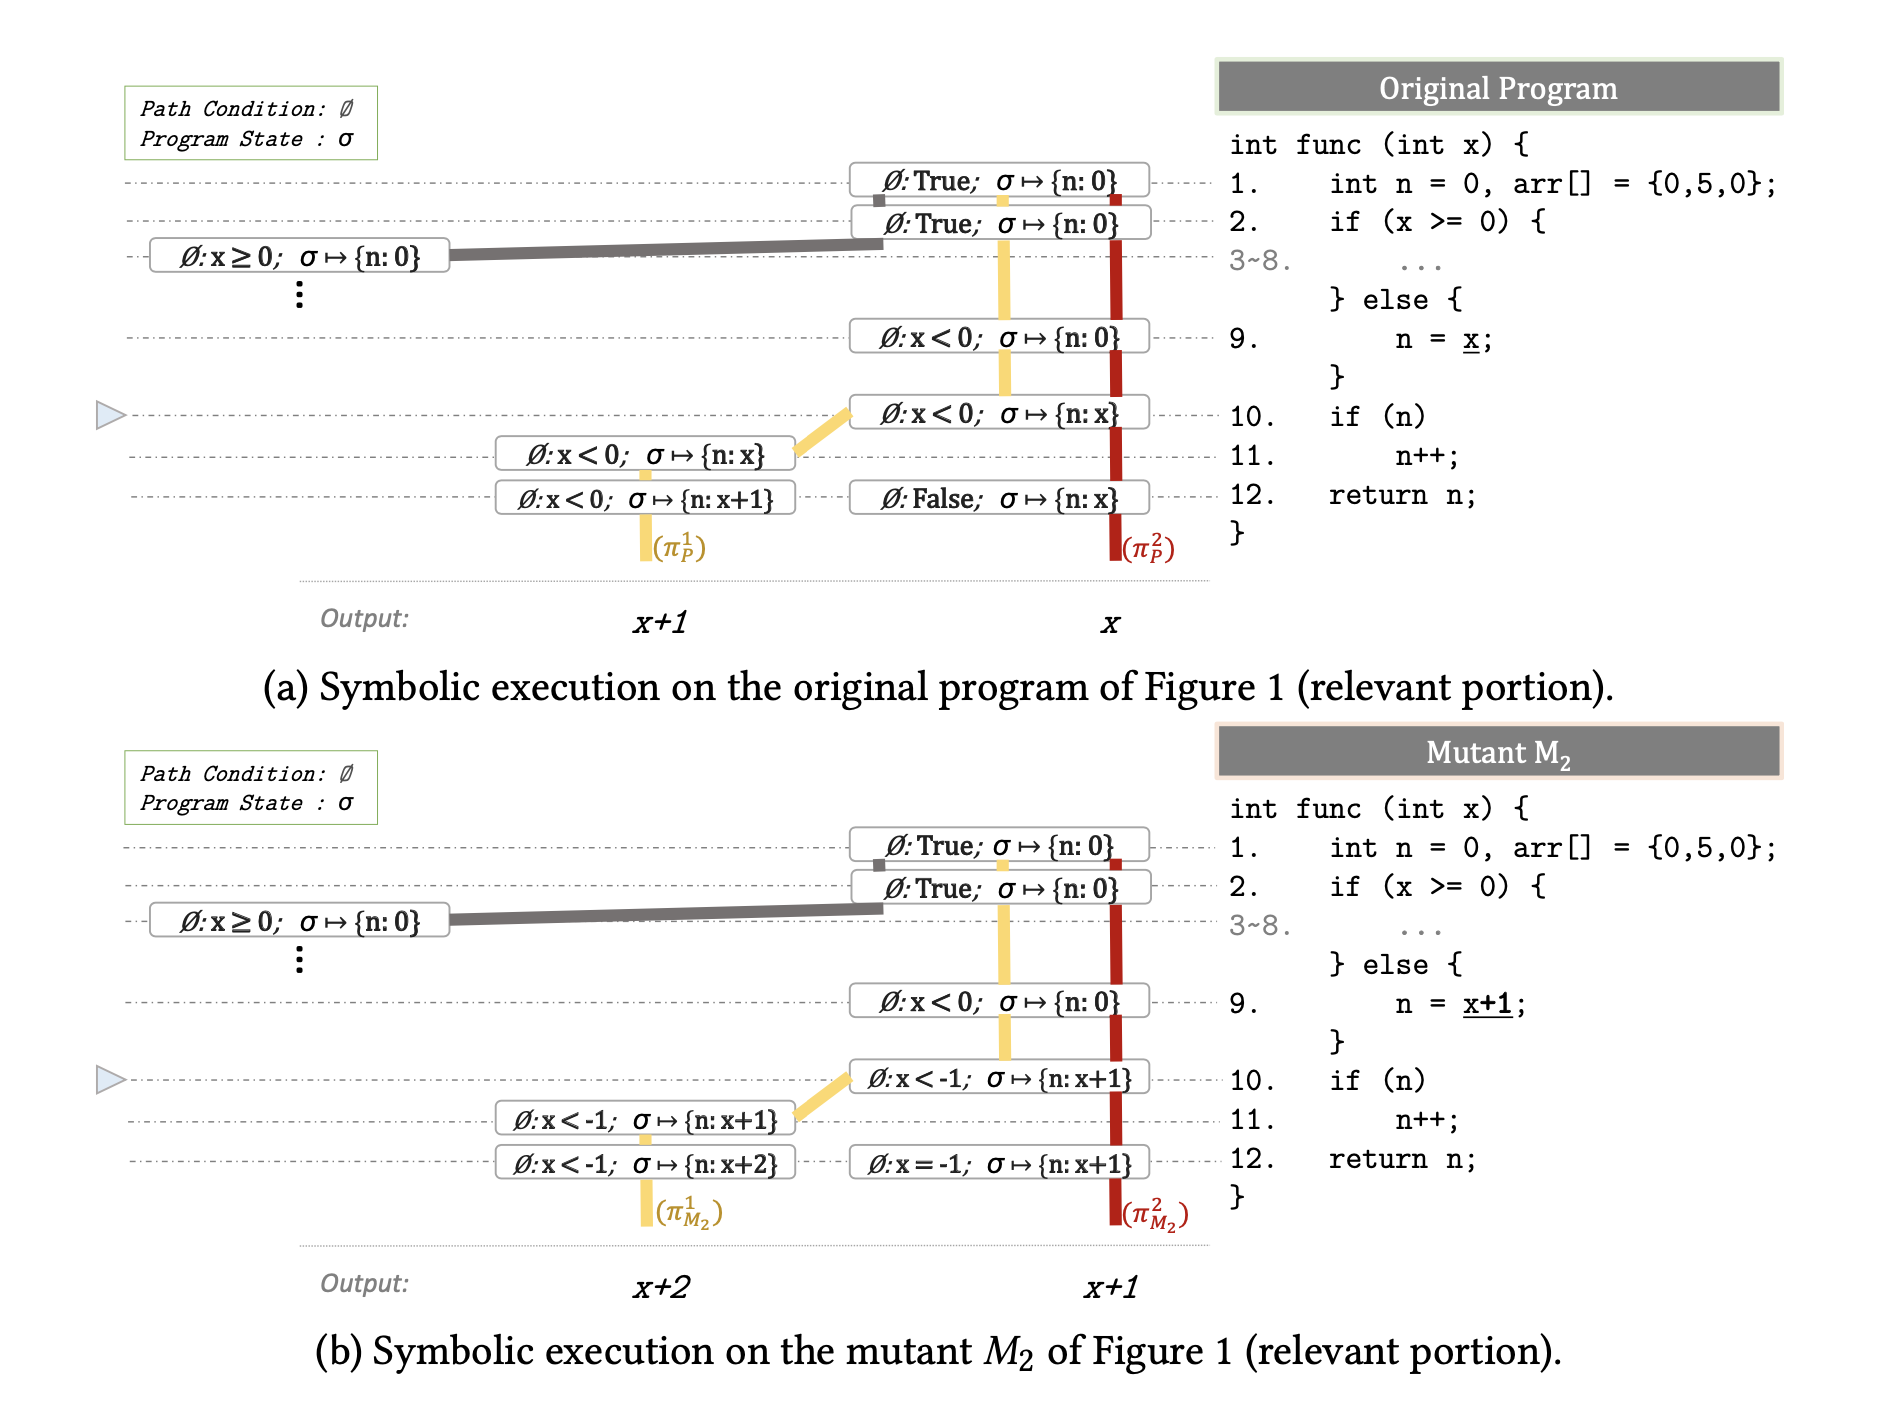
\includegraphics[width=\textwidth]{images/semu-example}
%\caption{SEMu example. Source: Chekam et al.~\cite{chekam2021killing}.}
%\label{fig:semu-example}
%\end{center}
%\end{figure}
%
%Figure~\ref{fig:semu-example} introduces an example of \INDEX{dynamic symbolic execution}, sub-figure (a) shows the symbolic execution for the original program, while (b) shows the symbolic execution process for the mutant version. In order to generate test inputs that kill a mutant, the technique applies symbolic execution to a program $P$ and to its respective mutant $M_2$, to produce their respective symbolic paths. In a second step, the technique solves the formula $kill(\pi_P, \pi_{M_2})$ to generate the test inputs that kills $M_2$ and goes through $\pi_P$ in $P$ and through $\pi_{M_2}$ in $M_2$. 
%As shown in Figure~\ref{fig:semu-example}, symbolic execution on the original program leads to the paths $x < 0$ and $False$, with the respective outputs $x + 1$ and $x$.
%Instead, the symbolic execution on the mutant leads to paths $x < -1$ and $x = -1$, with outputs $x + 2$ and $x + 1$.
%
%Consequently, the only feasible path that targets mutant $M_2$ is the following:
%
%\begin{equation}
%	kill(\pi_{P}^{1}, \pi_{M_2}^{1}) = ((x < 0) \wedge (x + 1 \neq x + 2) )
%\end{equation}
%
%Where the solution to $kill(\pi_{P}^{1}, \pi_{M_2}^{1})$ is $x = -2$.



To speed-up test generation, SEMu integrates a number of optimizations:
\begin{itemize}
	\item \INDEX{Meta-mutation}: all mutants are encoded into a single program called meta-mutant (in FAQAS, we extended it at source code level), the mutant is selected through a branching statement named mutant choice statement.
	\item \textbf{Discarding non-infected mutant paths}: mutant paths failing to infect the program state are discarded immediately.
	\item \textbf{Heuristic search}: stop exploration of a path after $K$ transitions, and solve the kill formula.
	\item \textbf{Infection-only strategy}: Generates test inputs by aiming only at mutant infection.
\end{itemize}

%\DONE{I have the impression that none of the following heuristics are currently used in FAQAS. I would write that we indicate which heuristics are not feasible and which one may be investigated in follow-up activities.}

%To reduce execution time further, SEMu also introduces a list of parametric heuristics that can be controlled by the user; this set of heuristics help to define which paths to explore and in general, the test generation process:

%%\DONE{please use "test cases" not "tests"}
%
%\begin{itemize}
%	\item \textbf{Controlling for reachability} (seeded symbolic execution): This heuristic consists of executing the original program up to a given path using the same inputs provided by existing test cases; the use of concrete inputs helps symbolic execution to quickly prune paths that are infeasible or does not reach the mutant. This feature is inherited from KLEE.
%	%a explore paths in seeded  mode up to a given length. 
%	
%%	\DONE{You are not explained what t does. "This heuristic consists of executing the original program up to a given path using the same inputs provided by existing test cases; it generates symbolic inputs only for...  For its implementation SEMu relies on a feature provided by KLEE"}
%	% This heuristic quickly prunes paths that are infeasible or does not reach the mutant. 
%	
%%	\DONE{Please refine what I wrote in the following. You were not explicitly clrifying hat the problem is.}
%	
%	We do not integrate this feature in the FAQAS framework because of two reasons. 
%	First, SEMu can deal only with test cases for batch programs (i.e., providing arguments to the main function of the software under test), which is different from our context where we either have unit or integration test cases implemented in a specific programming language, or we have complex system test cases simulating communication from ground to orbit through network and a simulator. 
%	Second, in our context, because of the complexity of the SUT we can generate unit test cases but not integration or system level ones. The main difference between such test cases is the entry point, for unit test cases it is the function under test, for integration or system test cases it is a function different than the function under test. Consequently, implementing such solution would require the implementation of additional technology to map the seeds collected for test inputs with different entry points, which is not provided by KLEE.
%
%	\item \textbf{Controlling for propagation}: This heuristic consists of controlling where and how often to verify whether the execution path has propagated the infection (i.e., an erroneous state with respect to the original program) after the execution of the mutated statement; if the mutation does not propagate the infection, the sufficiency killing condition will not be met, and thus it makes sense to prune these paths to decrease the symbolic search space.
%	% sometimes an infected program state fails to propagate the infection to the outputs, these states should be quickly discarded. 
%
%%	\DONE{Rewrite the sentence, unclear}
%	
%	For controlling the propagation of the infected state, SEMu introduces the following four parameters:
%	\begin{itemize}
%%		\item \DONE{(Comments are put above the problematic item) Unclear. Do you want to say that it consider checkpints with a predefined distance? Pleas write complete sentences sbject-verb-object.}
%
%		\item \textbf{Checkpoint Window}: This parameter determines the distance between checkpoints, where checkpoints are program locations with a branching statement. 
%
%		%\DONE{What are the criteria to discard a branch?}
%		At every checkpoint SEMu can (1) discard the branches that failed to propagate the infection, (2) generate tests based on the current states. Not used in FAQAS because we deal with unit testing (i.e., we test the mutated function).
%		
%		%\DONE{There is no more time for investigation, no? Explain why we discard it then.}
%		\item \textbf{Propagating Proportion}: This parameter specifies the percentage of branches that are kept to pursue the exploration. The use of this parameter requires additional investigation, to be investigated in follow-up projects.
%
%
%		%\DONE{You write "these branches", which branches? If all teh heuristics concern finding branches you need to specify above.}
%		%\DONE{To be investigated no}
%		\item \textbf{Propagation Selection Strategy}: While \textbf{Propagating Proportion} specifies the percentage of branches to be selected, this parameter determines how these branches are selected, particularly it can be done (1) randomly, or (2) selecting the branch that is closer to the output. 
%
%		Even though, the random strategy works better with batch programs according to literature~\cite{chekam2021killing}, we deal with unit tests for large programs. 
%
%%		\DONE{Why}
%		\item \textbf{Minimum Propagation Depth (MPD)}: This parameter specifies how many checkpoints should pass before generating the tests. We do not use this parameter in FAQAS (\texttt{MPD = 0}), since this enable SEMu to generate inputs quickly, and thus to save further computation time. 
%	\end{itemize}
%
%%	\DONE{Do not require for dong what? Complete the sentence. Who is the subject?}
%	\item \textbf{Controlling the cost of constraint solving} (no state difference): This heuristic consists of not requiring the state of the original program and the mutant to be different to solve the kill formula. The heuristic is not used in FAQAS, since it lowers the chances of killing a mutant. 
%
%	%\DONE{Unclear. Who is the subject?}
%	\item \textbf{Controlling the number of attempts} (number of tests per mutant): This heuristic specifies the number of tests to be generated for each mutant. Based on the idea that a test can kill multiple mutants. The use of the heuristic in the FAQAS context requires further investigation, to be addressed in follow-up projects. In the meanwhile, we generate only one mutant a time.
%
%\end{itemize}



\subsection{Test Generation based on Evolutionary Computation}

Test generation approaches based on \INDEX{evolutionary computation} typically rely on population-based meta-heuristic optimization algorithms~\cite{harman2011strong}. 
They search for program inputs that could kill mutants under the guidance of a fitness function~\cite{harman2011strong}. 
The main research contribution of these methods is the definition of fitness functions that capture the killing conditions of a mutant and identify test inputs that satisfy those conditions.

The \INDEX{fitness function} captures the killing conditions of a mutant. For instance, Ayari et al.~\cite{ayari2007automatic} proposed to use an evolutionary approach based on \INDEX{ant colony optimization} (ACO) for automatic test input data generation on mutation testing. The ACO is an optimization algorithm inspired by the behavior of ants, it is based on the ants ability to find the shortest path between their nest and the food source. In the study by Ayari et al.~\cite{ayari2007automatic}, the approach takes an existing test case and produces a new test case by slightly modifying its inputs. 
%F: you have to provide more details what does it mean "close"?
The fitness function measures the distance between the mutated statement, and the statement reached by the new test case (e.g., the reachability condition). More precisely, the distance is defined as the number of basic blocks between the two statements in the program's control flow graph.
Papadakis et al.~\cite{papadakis2011automatically}, instead, rely on fitness functions that capture the distance between mutated statement and the statement covering the branches of the different mutations (e.g., the necessity condition).

Fraser and Arcuri~\cite{fraser2015achieving} propose to use distinct distance metrics tailored to the specific operator used to generate the mutants.
%F: we need more examples for multiple operators. Also, you should clarify why distinct metrics are needed
This tailoring is needed because the \EMPH{necessity killing condition} relies on changes in the program state and the execution of a mutated statement does not guarantee that the program state had been changed (i.e., values on the stack are different at the mutation point).
%Fabrizio: it was not comprehensible
%mutation operators change the program state, and in other cases the program state remains unchanged. Because of this, distinct metrics for measuring distance for each operators needs to be defined.
%\DONE{I cannot undertsand the following, we can ignore it.}
%\DONE{In the following, I added a sentence in paranth. Is it correct? YES}
For example, the \textit{deletion operator}, which removes a statement, may or may not change the program state, depending on the semantic of the removed sentence \CHANGEDTWO{(e.g., a logging instruction does not alter the program state)}. In case the mutation effectively changes the program state the distance is set to 0, otherwise the given value is 1.
% For example if the \textit{deletion operator} changes the program state (i.e., values on the stack are different at the mutation point) the distance is 0, otherwise the given value is 1. 
In the case of the \textit{insert unary operator}, which adds or subtracts 1 to a numerical value, the operator always change the program state, so the distance is set to 0 when the statement is reached. 
% For this reason, the mutants produced by this operator always affect the program state, so the distance is always 0 when the statement is reached.

Instead, in the case of the \textit{replace variable operator}, which replaces a specific variable with all other variables of the same type in the program scope, the distance is set to 0 only if the values of the variables being exchanged are different before executing the statement, otherwise it is set to 1.

\subsubsection{\REVTWO{C37}{Generation of test oracles}}
\label{sec:oraclesGeneration:codeDriven}

The automated generation of test oracles is a research topic that goes beyond the specific needs of mutation testing~\cite{Barr:Oracles:15,OLIVEIRA:Oracles:2014}.

Fraser et al. provide an overview of existing approaches for the automated generation of test oracles that have been integrated into existing test case generation tools~\cite{fraser2011mutation}.
A common solution consists of the automated synthesis of assertions for the test case. These assertions reflect the output generated by the function under test when it is exercised with the automatically generated input. 
For example, Line~6 in Listing~\ref{isPositiveOracle} shows the oracle that can be automatically generated for the function analyzed in Listing~\ref{example} (i.e., function \emph{isPositive}). The oracle, in this case, consists of an assertion verifying that the value generated by function \emph{isPositive} matches the value '1', which is the value observed during test generation for the input value '0'. This is the approach implemented by Riener et al.~\cite{riener2011test}, who generate assertions that verify variables that present different values between the original and the mutated executions.

\begin{minipage}{15cm}
\begin{lstlisting}[style=CStyle, caption=Automatically generated oracle for function 'isPositive'., label=isPositiveOracle]
void test () { 
	int numSymbolic = 0;
 	
 	int ret = isPositive(numSymbolic); 
	
	assert( ret == 1 ); 
}
\end{lstlisting}
\end{minipage}

Randoop~\cite{PachecoLEB2007} allows annotation of the source code to identify observer methods to be used for assertion generation. Orstra~\cite{Xie:2006} generates assertions based on observed return values and object states.
DiffGen~\cite{Taneja:2008} extends the Orstra approach to generate assertions from runs on two different program versions.

A well known limitation of automatically generated assertions that reflect the actual values observed during execution is that
they need to be validated. More precisely, we need to ensure that the values expected by the assertions do not reflect a failure triggered by the test case (e.g, an erroneous value being returned). Such validation activity is typically performed manually by the engineers because it should be based on domain knowledge and system specifications. 
Specifications are generally written in natural language because, to reduce development costs, only few components of the system are specified using formal languages. For this reasons the automated verification of such assertions is infeasible.

Approaches that support engineers in the analysis of generated oracles exist and might be considered to speed up the process~\cite{Staats2012,PastoreICSE2015}. For example, 
Staats et al.~\cite{Staats2012} identify the subset of variables to be verified by oracles in order to maximize the fault finding potential of the testing process.
%with respect to the cost of manually verifying the correctness of each generated assertions. 
First, they generate a collection of mutants from the SUT. Second, the test suite (automatically generated) is run against the mutants using the original system as the oracle. Third, they select the variables to verify in test oracles by focussing on those variables that show different values in the original and the mutated version.

ZoomIn.~\cite{PastoreICSE2015} automatically identifies suspicious assertions. These are assertions that verify data that is generated by functions showing anomalies during test cases executions. Anomalies are detected by automatically deriving pre- and post-conditions of the functions of the SUT based on the data recorded during the execution of a manually implemented test suite. Anomalies consist of function executions that violate such pre- and post-conditions. 
%To rank unsafe assertions, ZoomIn takes into consideration the number of violations of pre- and post-conditions produced by the related program variables. However, not all the constraint violations are equally important. Since erroneous behaviors are not frequent in adequately tested software, ZoomIn weights each constraint according to the number of times the constraint has been violated. The frequently violated constraints are likely imprecise constraints that erroneously detect legal values as anomalous values, while constraints that are seldom violated are likely to carry useful information. ZoomIn captures this aspect with the uniqueness score. 
%Also, ZoomIn associates the assertions with a score, the suspiciousness score, that represents the likelihood the assertion is wrong. The suspiciousness score of an assertion depends on both the number and the uniqueness scores of the related constraints that are violated. Intuitively the highly scored assertions, i.e., the most suspicious assertions, are the ones associated with several constraint violations with high uniqueness scores.
%To keep the inspection effort low and the effectiveness high, developers are assumed to inspect only the top assertions in the ranking. Results show that inspecting the top five unsafe assertions is enough to discover several faults without wasting time inspecting too many correct assertions.

% measure how often each variable in the system reveals a fault in a mutant and?based on this information?we rank variable effectiveness in terms of fault finding. Finally, we estimate? based on this ranking?which variables to include in the oracle data for an expected value oracle. The underlying hypothesis is that, as with mutation-based test data selection, oracle data that is likely to reveal faults in the mutants will also be likely to reveal faults in the actual system under test. This oracle data selection process is completely automated and requires no manual intervention. Once this oracle data is selected, the tester defines expected values for each element of the oracle data. Testing then commences with a?hopefully?small and highly effective oracle.


%According to recent survey on the topic, test oracles can be divided in three categories:
%oracles defined though a \INDEX{specification language} (i.e.,  is a notation for defining a specified test oracle, which judges whether the behaviour of a system conforms to a formal specification).

%  test oracles can be derived (Section 5);
%  test oracles can be built from implicit information
%(Section 6); and

%In the context of code-driven metamorphic testing
%
%
%
%Staats2012

\subsection{Summary}

Among all the approaches for test input generation, SEMu is the most advanced one. However, it does not integrate solutions to automatically generate oracles. Solutions for generating oracles are at their infancy and cannot be considered ready for integration into the FAQAS toolset.




% !TEX root = Main.tex

\section{Data-driven Mutation Testing}
\label{sec:testGenerationData}



Although the literature does not address the problem of automatically generating test cases for data mutation testing, in this section we provide references to work that can be reused for this purpose.
We discuss both the generation of \INDEX{test inputs} and \INDEX{test oracles}.
Concerning the generation of test inputs, we group the applicable approaches according to the type of models used to specify the data to be generated: \INDEX{UML models}, \INDEX{grammars}, \INDEX{block models}, and \INDEX{no models}.

Automated test inputs generation aims to automatically generate data that can be altered through a mutation operator.
In the context of system and integration testing, which is the target of data-driven mutation testing, test input data is provided through input interfaces. However, since data-driven mutation is applied to data exchanged different communication layers, including input interfaces and interfaces used for the communication among internal components, we may observe two possible situations. First, the data targeted by mutation testing coincide with the input data (i.e., it was not transformed internally). Second, the data targeted by data mutation is the result of a transformation of the input data. We thus need to consider both the two cases when discussing related work.

\subsection{UML models}
%model-based fuzzying and

%In the case of modelling based on UML models, a data mutation operator may not be applied during mutation testing when the type of data that it is supposed to alter is not observed during the execution of the test cases.
%For example, in the case of the data model in Figure~\ref{fig:dataModel}, we may not be able to apply the operator \emph{Attribute Replacement with Random} to the attribute \emph{destinationId} of class \emph{GpsrPacketHeader} if all the test cases contain messages with \emph{SarPacketHeaders}.



When the data exchanged on the communication layer targeted by mutation testing coincide with the input data, existing approaches based on constraint-solvers can be adopted.
These approaches rely on a formal or semi-formal specification of the structure of the input data and the constraints among data fields.
Some techniques target the generation of inputs whose data structure had been specified using a UML class diagram where the relations among data fields have been captured using OCL constraints. The data structure model is a UML class diagram and resembles the one reported in Figure~\ref{fig:dataModel}. The OCL language is instead used to capture all the constraints among data fields. Existing techniques in this category work by generating class diagram instances that satisfy a set of given OCL constraints by executing appropriate constraint solvers after having transformed the OCL constraints into other formalisms such as \INDEX{Alloy models}~\cite{Uml2alloy}, \INDEX{constraint satisfaction}~\cite{EMFTOCSP}, \INDEX{SMT}~\cite{Przigoda2016}, or \INDEX{SAT} problems~\cite{Soeken2011}.

\begin{figure}[t!]
 \centering
   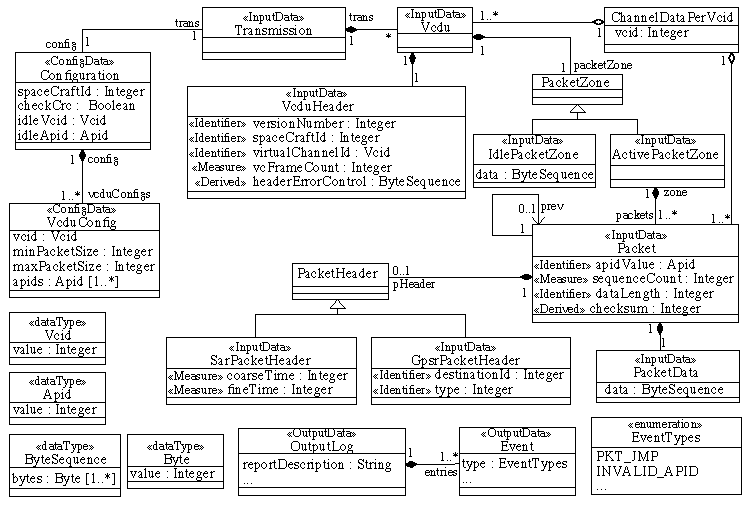
\includegraphics{images/classDiagramSmall}
     \caption{Simplified input data model taken from~\cite{di2015evolutionary}.}
     \label{fig:dataModel}
\end{figure}

Other approaches, instead, work with models specified in formats other than UML class diagrams:
\INDEX{Java classes}~\cite{Boyapati-KORAT-ISSTA-2002,gligoric2010test}, \INDEX{constraint logic}~\cite{Senni-CPLgeneration-TAP-2012}, \INDEX{Alloy}~\cite{Khurshid-SpecificationBasedTesting-ASE-2004}, or \INDEX{Z specifications}~\cite{Horcher-Z-1995}.
These techniques have been proven to be effective for testing software systems that process classical data structures like trees.
Alloy is a modelling language for expressing complex structural constraints~\cite{Jackson:Alloy:2002},
which has been successfully used to generate test inputs for testing object-oriented programs~\cite{Khurshid-SpecificationBasedTesting-ASE-2004}.
Korat, instead, is a technique that enables the generation of data structures to test Java programs~\cite{Boyapati-KORAT-ISSTA-2002}. Given a bound to the input structures (i.e., the maximum number of instances for each class to be used), Korat exhaustively generates all the nonisomorphic structures that are valid.
Some of the limitations of Korat include requiring the definition of an imperative predicate that evaluates the correctness of the generated structure, which could be complex in the case of complex data models, requiring the manual definition of an input bound for each non primitive attribute or association, which might be particularly expensive in case of complex data structure,  not dealing with constraints defined over integers.
A more efficient, black-box test generation approach is UDITA~\cite{gligoric2010test}.
What contributes to the efficiency of UDITA is the combination of both generator methods and predicates.
Generator methods are used to build instances of the data structure, while predicates are used to validate the generated instances. UDITA relies upon the Java Path Finder model checker~\cite{Visser-JPF-2004} to generate all the instances that satisfy the given predicates. However, the implementation of these generator methods that define the complete structure of a complex data model instance and lead to realistic test inputs can be quite expensive.

A common limitation of solutions based on constraint-solvers is their scalability~\cite{di2017augmenting}. In the context of mutation testing, where existing test inputs are available, a possible solution to address the scalability problem may consist of generating new test inputs by \EMPH{regenerating only portions of existing test inputs}.
For example, Di Nardo et al.~\cite{di2017augmenting} automatically generate test inputs for new requirements by adapting existing field data.
This is achieved by combining model transformations with constraint solving.
%% as shown in Fig.~\ref{fig:DiNardo}.
%Model transformations enable the partial reuse of existing field data, while constraint solving allows for the generation of missing data. The approach requires a model of the structure of the data provided by using an UML class diagram with OCL expressions capturing the constraints among data fields. In the case of Di Nardo et al., the missing data correspond to new data types and constraints introduced after updating the requirements of the software under test. In the context of mutation testing, these may correspond to data types not observed during the execution of the test suite.
%In Step 1, a chunk of data is loaded in memory as an instance of the original data model (Original Model Instance).
%A dedicated parser is used for that purpose.
%In Step 2, a model transformation applied to the Original Model Instance is used to generate an instance of the Updated Data Model. The result is an instance of the Updated Data Model that is incomplete (Incomplete Model Instance).
%It contains only the information that can be directly derived from the Original Model Instance:
%instances of classes and attributes that have been introduced in the Updated Data Model are missing from the Incomplete Model Instance (these instances are the ones generated in the next steps of the algorithm).
%In Step 3, UML2Alloy~\cite{Uml2alloy} is used to generate an Alloy model that corresponds to the class diagram and the OCL constraints of the data model; the Alloy Analyzer~\cite{AlloyWeb} is then used to generate  valid instances of the updated data model by means of constraint solving.
%Finally, in Step 4, to generate the concrete test inputs to be processed by the software under test (e.g. a binary file), the content of the Valid Model Instance is written in the format processed by the software under test through a dedicated encoder.
Despite empirical results show a huge performance gain with respect to traditional constraint-based approaches, the need for dedicated parsers to translate existing test inputs into class diagram instances may limit the applicability of the approach. Also, the available test inputs may not enable the generation of all the inputs data needed.

%\begin{figure}[t!]
%  \centering
%    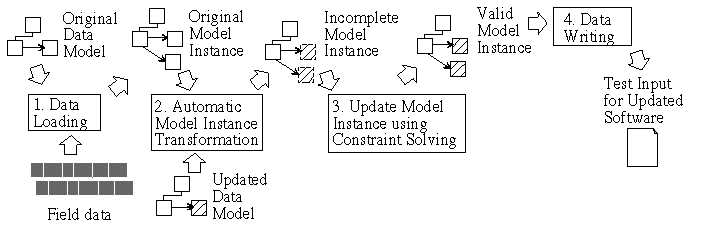
\includegraphics{images/DiNardoTOSEM}
%      \caption{Automatic generation of test inputs for new data requirements proposed by Di Nardo et al~\cite{di2017augmenting}.}
%      \label{fig:DiNardo}
%\end{figure}

Other approaches address the scalability problem by relying on \INDEX{hybrid input generation approaches}~\cite{soltana2019practical}.
For example, PLEDGE~\cite{soltana2019practical} combines metaheuristic search and Satisfiability Modulo Theories (SMT~\cite{SMT:2011}) to generate UML instance models from UML class diagrams annotated with OCL constraints. It  works by using the Negation Normal Form (NNF~\cite{NNF:2001}) to represent all the constraints derived from the UML data model. Different subformulas that build the NNF formula are then solved by combining metaheuristic search and SMT. Metaheuristic search is used to handle subformulas whose satisfaction involves structural tweaks to the instance model, i.e., additions and deletions of objects and links. SMT is used with subformulas involving only primitive attributes, i.e., attributes with primitive types.


When the data exchanged on the communication layer targeted by mutation is the result of a transformation of the input data, the only applicable solution consist in the application of approaches that generate inputs from scratch. By generating a large number of inputs that include instances for all the classes of the data model, these approaches may, in principle, lead to the generation of required data by internal components. However, without means to drive the generation of such data, the application of UML-based test input generation approaches in these situation is likely to be inefficient.

%Despite this approach enables efficient generation of test inputs from scratch, it may still require dedicated parsers for the con

\subsection{Grammars}

When grammars are used to model the input, \INDEX{grammar-based test input generation} approaches relying on the expansion of the production rules of the grammar can be adopted~\cite{fuzzingbook2019:GrammarFuzzer}.
Available tools are shown in Table~\ref{table:grammarGeneration}.

%Listing~\ref{TestJSON} shows the inputs generated by \emph{Coverage-based Fuzzer}~\cite{fuzzingbook2019:GrammarFuzzer} to cover all the production rules and terminals of the grammar (one input per line). Listing~\ref{TestJSON} shows that these automatically generated inputs are difficult to read. For example, for a human, is more difficult to  read Listing~\ref{TestJSON}  than Listing~\ref{JSONfile}.
%
%% !TEX root = ../MutationTestingSurvey.tex
\begin{minipage}{14cm}
\footnotesize
\begin{lstlisting}[caption=Test Cases covering the JSON grammar shown in Listing~\ref{JSONgrammar}, label=TestJSON]
 true 
 null 
 false 
 { "k" : [ "o9*i`BM+Lw^jY7EUyX3e_}(1~$TJS2carZVND@zfh5%qObgu<;K CFW=dm&.[:)xl#'{H8I|]GAQPn,6-v>t0p?s4R!k/tOr" ] } 
 -20.538 
 [ ] 
 { } 
 -7e+9 
 6.13E4 
 90E-008 
 { "" : [ true ] , "" : false , "" : true , "" : true , "" : true } 
 [ [ false ] , true ] 
\end{lstlisting}
\end{minipage}

\begin{table}[h]
\caption{List of tools for grammar-based inputs generation.}
\label{table:grammarGeneration}
\begin{center}
\tiny
\begin{tabular}{|p{2cm}|p{2cm}|p{2cm}|p{7cm}|}
\hline
\textbf{Name}&\textbf{Grammar}&\textbf{Licence}&\textbf{Description}\\
\hline
GramTest~\cite{GramTest}& BNF&Apache 2.0&Java-based tool that allows you to generate test cases based on BNF grammars. It covers all the production rules of the grammar.\\
\hline
Fuzzingbook Grammar Coverage-based Fuzzer~\cite{fuzzingbook2019:GrammarFuzzer}& BNF & MIT &Python tool that implements production rules coverage. It implements the Shortest Path Selection~\cite{Burkhardt:TestFromSyntax} optimization.\\
\hline
GP~\cite{GPlib,Kifetew:GBTest:2017}& Annotated BNF & Proprietary& Tool for the automated generation of inputs from Stochastic Context Free Grammars. Implemented on top of genetic programming algorithms. https://selab.fbk.eu/kifetew/downloads/gplib-607.jar\\
RIDDLE~\cite{ghosh1998testing}&BNF& Proprietary& Tool that adopts a grammar to describe the format of inputs; based on the grammar, random and boundary values are generated for tokens representing input parameters.\\
\hline
\end{tabular}
\end{center}
\end{table}%

Among existing approaches, \INDEX{Parser-Directed Fuzzing} (hereafter, \emph{pFuzzer}) aims at producing valid inputs for input parsers~\cite{mathis2019parser}. The challenge is to cover all the lexical and syntactical features of a certain language. The approach systematically produces inputs for the parser and tracks all the comparisons made; after every rejection, it satisfies the comparisons leading to rejections, effectively covering the input space.
Evaluated on five subjects, from CSV files to JavaScript, the \emph{pFuzzer} prototype covers more tokens than both lexical-based (AFL) and constraint-based approaches (KLEE).


Similarly to the case of UML-based test case generation approaches that generate inputs from scratch, these grammar-based approaches can be adopted when the communication layer targeted by mutation testing is either the input layer or an internal layer.However, they may suffer of inefficiency problems; in additions, grammar can be unlikely used to model the types of data processed by space software.

%\cite{grammar:survey}

\subsection{Block-models}

Among the existing toolsets based on block-models, \INDEX{Peach} is the only one which supports the automated generation of test data. However, it's implementation simply generates random data, the process is referred to as
\INDEX{blind fuzzing}\footnote{https://wiki.mozilla.org/Security/Fuzzing/Peach$\#$Creating\_a\_Data\_Model}.


\subsection{No models}


The generation of test inputs without the need of data model is typically driven by code coverage. A representative solution is given by AFL.
% which has been introduced in Section~\ref{sec:data_operators}.

More in general, approaches that address the problem of automatically testing programs that process structured data can be adopted for this purpose~\cite{Kiran:2008,Braione:2017,Braione:2018}. For example, SUSHI~\cite{Braione:2018} is a tool that aims to cover test objectives that depend on non-trivial data structure instances.
It relies on symbolic execution to generate path conditions that capture the relationship between program paths and input data structures. The path conditions are then translated into fitness functions to enable testing based on meta-heuristic search. A solution for the search problem is a sequence of method invocations that instantiates the structured inputs to exercise the program paths identified by the path condition.

\subsection{Automated Generation of Test Oracles}
\label{sec:oracles:dataMutation}

In the case of data-driven mutation testing, solutions for the \INDEX{automated generation of oracles} that consist of assertions verifying the output of the software under test (see Section~\ref{sec:oraclesGeneration:codeDriven}) might still be applied. However, considering that data-driven mutation testing is more likely adopted in the context of system-level testing, where inputs consist of complex, structured data, the generation of test oracles using techniques built for unit testing is likely infeasible in this context.

Possible solutions may consist of approaches that verify the correctness of the log files generated during the execution of the program~\cite{Pastore:ISSRE:08,Pastore:TKT:17}.
Given a set of log files (or execution traces) generated during valid executions, these approaches can derive \INDEX{finite state automata} (FSAs) that capture the sequences of events and data-flow observed in valid executions. The derived FSAs can be used to verify if new executions match the inferred models. More precisely, they enable the automated detection of invalid sequences of events and data-flows. Despite none of these approaches had been applied in the context of data-driven mutation testing, traces collected from multiple runs of a same test case might be used to derive an FSA that captures the behaviour of a single test case. By relying on multiple traces collected from a same test case we can leverage the generalization power of the inference engines used to generate the FSAs; these inference engines, for example, can automatically recognize and filter out variable elements such as timestamps. The inferred FSAs could thus then be used as oracles for newer executions of the generated test cases. Such approaches have shown to be effective in detecting both functional failures~\cite{Pastore:ISSRE:08} and performance problems~\cite{Pastore:TKT:17}.

% !TEX root = MAIN.tex
\clearpage
\subsection{Benchmark of State-of-the-art Data-driven Mutation Testing Toolsets}
\label{sec:toolsComparisonDataDriven}

This section describes an evaluation we conducted to identify a data-driven mutation testing tool applicable to space context. In particular, we assessed the \INDEX{Peach Fuzzer toolset}.

% description of the toolset

% !TEX root = ../MutationTestingSurvey.tex

\begin{table}[h]
\begin{center}
\footnotesize
\CHANGEDTWO{
\begin{tabular}{|p{5cm}|p{9cm}|}
\hline
\textbf{Operator Name}&\textbf{Description}\\
\hline
ArrayVarianceMutator&Change the length of arrays. Given L the original length of the array, the length is changed in range L-N to L+N.\\
ArrayReverseOrderMutator&Reverse the order of an array.\\
ArrayRandomizeOrderMutator&Put array elements in random order.\\
DWORDSliderMutator&Slides a DWORD through the blob.\\
BitFlipperMutator&Flips a given \% of bits in blob. Default is 20\%.\\
BlobMutator&Randomly grows a Blob block or shrinks it.\\
DataTreeRemoveMutator&Remove nodes from data tree.\\
DataTreeDuplicateMutator&Duplicate a node's value starting at 2x through 50x.\\
DataTreeSwapNearNodesMutator&Swap the data of two nodes that are near each other in the data model.\\
NumericalVarianceMutator&Produce numbers that are defaultValue - N to defaultValue + N.\\
NumericalEdgeCaseMutator&Replace with random numbers of appropriate correct size.\\
FiniteRandomNumbersMutator&Produce a finite number of random numbers for each \emph{Number} element.\\
NumericalEvenDistributionMutator&Generate numbers evenly distributed through the total numerical space of the number range.\\
NullMutator&Does nothing, just test the data produced by the fuzzer.\\
PathValidationMutator&Does not mutate. Used to trace path of each test for path validation.\\
SizedVarianceMutator&Change the length of sizes to count - N to count + N.\\
SizedNumericalEdgeCasesMutator&Change the length of sizes to numerical edge cases.\\
SizedDataVarianceMutator& Change the length of sized data to count - N to count + N. Size indicator will stay the same.\\
SizedDataNumericalEdgeCasesMutator&Change the length of sizes to numerical edge cases.\\
StringCaseMutator&Change the case of a string.\\
UnicodeStringsMutator&Generate unicode strings.\\
ValidValuesMutator&Replace with random values other than the legal ones.\\
UnicodeBomMutator&Injects BOM markers into default value and longer strings.\\
UnicodeBadUtf8Mutator&Generate bad UTF-8 strings.\\
UnicodeUtf8ThreeCharMutator&Generate long UTF-8 three byte strings.\\
StringMutator&Generate a random unicode string, for each string node, one Node at a time.\\
XmlW3CMutator&Replace XML trees with invalid, non-well former, and valid (but random) XML trees.\\
PathMutator&Replace a path with an erroneous path generated according to 20 different rules.\\
HostnameMutator&Replace a hostname with an erroneous hostname generated according to 20 different rules.\\
IpAddressMutator&Replace an IP address with an erroneous IP address generated according to 20 different rules.\\
TimeMutator&Replace a time value with an erroneous value generated according to 3 different rules.\\
DateMutator&Replace a date with 60 predefined erroneous dates.\\ 
FilenameMutator&Replace a file name with an file name generated according to 10 different rules.\\
ArrayNumericalEdgeCasesMutator&This operator is not well documented in the source code of Peach.\\
BlobSpread&This operator is not well documented in the source code of Peach.\\
\hline
\end{tabular}
}
\end{center}
\caption{Mutation Operators for the opensource version of Peach~\cite{PeachMozilla}}
\label{table:PeachOperators}
\end{table}%

% !TEX root =  ../MAIN.tex

\begin{minipage}{15cm}
\begin{lstlisting}[language=XML, caption=Portion of a Peach data model., label=peach, mathescape=true]
<Number name="lfh_CompSize" size="32" endian="little" signed="false"/>
<Number name="lfh_DecompSize" size="32" endian="little" signed="false"/>
<Number name="lfh_FileNameLen" size="16" endian="little" signed="false">
    <Relation type="size" of="lfh_FileName"/>
</Number>
<Number name="lfh_ExtraFldLen" size="16" endian="little" signed="false">
    <Relation type="size" of="lfh_FldName"/>
</Number>
<String name="lfh_FileName"/>
<String name="lfh_ExtraField"/>
\end{lstlisting}
\end{minipage}



Peach~\cite{PeachMozilla,PeachFuzzer} is a fuzzing tool that relies on \INDEX{block models}~\cite{pham2016model,spike} to perform data mutations. In other words, Peach performs mutations by altering the data of an input according to a large, predefined set of rules. For example, Listing~\ref{peach} introduces a portion of a data model describing the properties of the Zip data format~\cite{zipformat}. 

Even though Peach is currently a proprietary software~\cite{PeachFuzzer}, the Mozilla Foundation maintains a community edition of the toolset~\cite{PeachMozilla}, the community edition implements basic features such as the fuzzing capabilities. The proprietary version of Peach instead provides features for automatic generation of test cases and detailed reports about the potential security threats of a software~\cite{PeachFuzzer}. The version we evaluated in this activity was the community edition provided by the Mozilla Foundation. We provide an overview of the mutation operators implemented by the Peach community edition in Table~\ref{table:PeachOperators}.

% what we did

In the assessment of Peach, we defined three criteria to understand its applicability to the space context software. The first criteria concerns assessing if the community edition of Peach does work and if it can be installed properly. The second criteria concerns its portability. Finally, the third criteria concerns assessing its compatibility with FAQAS case study systems.

Regarding the first criteria, we tested Peach by applying it to the \texttt{unzip} program, and zip file mutants with the fuzzing capabilities of Peach. For this objective we reproduced the steps indicated in~\cite{zipexample}. So, first, we generated a Peach Data Model for Zip data files, and then we specified a launcher that enables the complete mutation process.

Peach provides a monitoring infrastructure that enables the execution of the whole mutation process. The process consists of the following steps:
\begin{enumerate}
	\item Specifying the data model for the a data type into an XML file.
	\item Loading the data model into Peach.
	\item Generating a new mutant (i.e, a mutated input).
	\item Running the program taking as an input the generated mutant, and with the monitoring infrastructure enabled.
	\item If the program crashes the process is stopped.
	\item If the program does not crashes, the process goes back to step 3, performing a new mutation.
\end{enumerate}

In particular, we were able to generate mutants for the Zip data format, but we could not run the monitoring infrastructure since it had dependencies with graphical environments that prevent us to execute it properly.

Regarding the second criteria, and specifically its portability. We seek to integrate it into the case studies as a component of their software to mutate data once it is sent, basically the idea would be to intercept the methods that exchange data, and apply Peach directly to the variable containing the data.
During the evaluation, we discovered that Peach -mainly implemented in Python- can be used as a Python library, and that this library can be invoked to generate multiple mutants in a off-line mode.

% why it was discarded

Regarding the third criteria and its compatibility with our case studies, we conclude that its integration with embedded systems is unlikely to work, mainly because of the characteristics of our case study systems.
For example, the ESAIL case study system runs within a real-time operative system (i.e., RTEMS by Edisoft) that does not possess a filesystem. Therefore, integrating Peach into ESAIL is not feasible because it might affect the real-time performance of the application, and also because it will be necessary to implement a solution to port the Peach toolset into the ESAIL infrastructure.





% !TEX root = MAIN.tex

\chapter{The FAQAS approach}
\label{chapter:approach}

This chapter presents the theory and the methodology behind the toolset implemented by FAQAS.




% !TEX root =  Main.tex
\section{Code-driven Mutation Analysis: MASS}
\label{ch:mass:approach}

\subsection{Overview}
\label{sec:approach}

\begin{figure}[tb]
\begin{center}
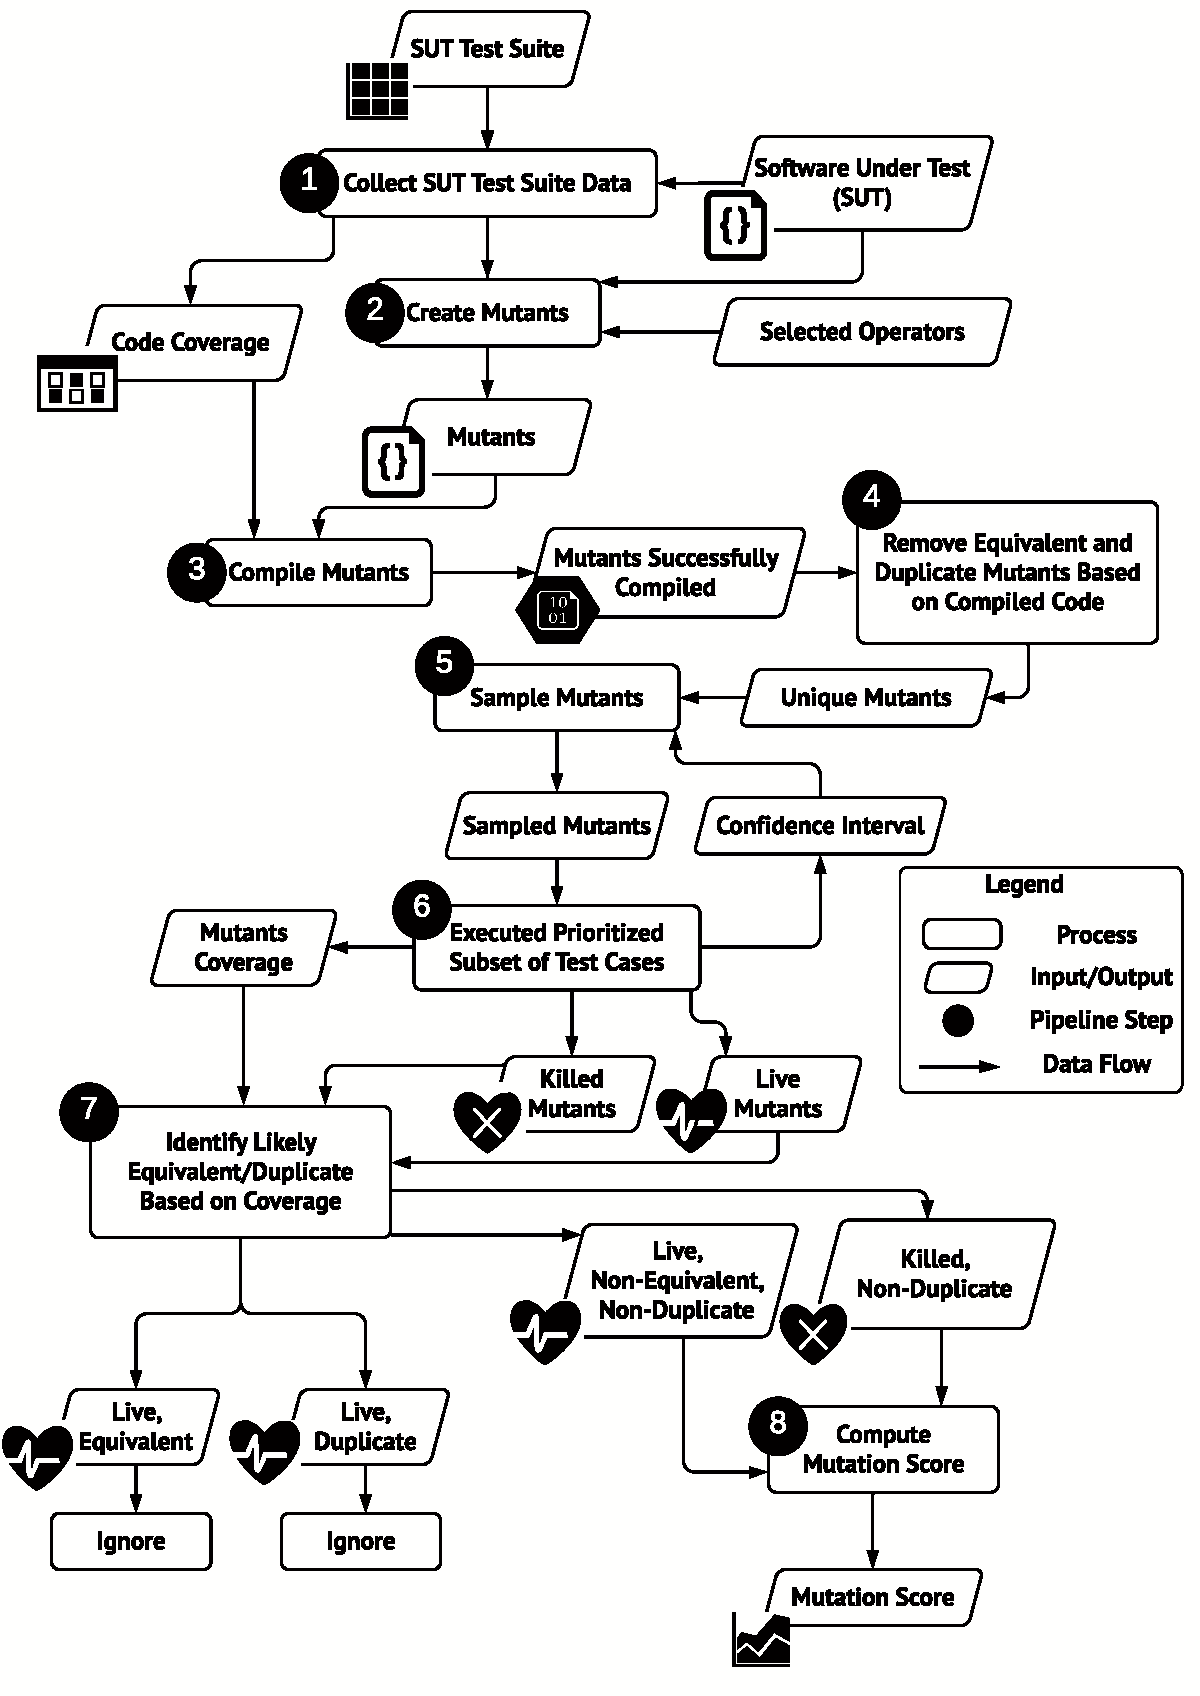
\includegraphics[width=0.6\textwidth]{images/Approach}
\caption{Overview of MASS}
\label{fig:approach}
\end{center}
\end{figure}

Figure~\ref{fig:approach} provides an overview of the mutation analysis process that we propose, \emph{Mutation Analysis for Space Software (\APPR)}. Its goal is to propose a comprehensive solution for making mutation analysis applicable to embedded software in industrial cyber-physical systems. \JMR{3.4}{The ultimate goal of \APPR is to assess the effectiveness of test suites with respect to detecting violations of functional requirements.}
 
\JMR{3.3}{Different from the mutation analysis pipeline presented in related work~\cite{papadakis2019mutation}, \APPR enables the integration of all mutation analysis optimization techniques that are feasible in our context to address scalability and pertinence problems (see Section~\ref{sec:back:summary}). 
\APPR consists of eight steps: (Step 1) Collect SUT Test Suite Data, (Step 2) Create Mutants, (Step 3) Compile Mutants, (Step 4) Remove Equivalent and Duplicate Mutants Based on Compiled Code, (Step 5) Sample Mutants,  (Step 6) Execute Prioritized Subset of Test Cases, 
(Step 7) Identify Likely Equivalent / Duplicate mutants Based on Coverage, and
(Step 8) Compute the Mutation Score. Different from related work, \APPR enables FSCI-based sampling by iterating between mutants sampling (Step 5) and test cases execution (Step 6). 
Also, it integrates test suite prioritization and reduction (Step 6) before the computation of the mutation score.
Finally, it includes methods to identify likely equivalent and duplicate mutants based on code coverage (Step 7).}
We describe each step in the following paragraphs. 

\clearpage
\subsection{Step 1: Collect SUT Test Data}

In Step 1, the test suite is executed against the SUT 
%software under test (SUT) 
and code coverage information is collected. 
More precisely, we rely on the combination of gcov~\cite{GCOV}
and GDB~\cite{GDB}, enabling the collection of coverage information for embedded systems without a file system~\cite{THANASSIS}.
% and Vector CAST~\cite{VectorCAST} 
%to record the number of times each line of code of the SUT has been exercised by a test case.

\subsection{Step 2: Create Mutants}

In Step 2, we automatically generate mutants for the SUT by relying on a set of selected mutation operators.
In \APPR, we rely on an extended sufficient set of mutation operators, which are listed in Table~\ref{table:operators}.
%In addition, in our experiments, we also evaluate the feasibility of relying only on the SDL operator, combined or not with OODL operators, instead of the entire sufficient set of operators.

% !TEX root =  ../Main.tex

\newcommand{\op}{\mathit{op}}
\newcommand{\ArithmeticSet}{ \texttt{+}, \texttt{-}, \texttt{*}, \texttt{/}, \texttt{\%} }
\newcommand{\LogicalSet}{ \texttt{&&}, \texttt{||} }
\newcommand{\RelationalSet}{ \texttt{>}, \texttt{>=}, \texttt{<}, \texttt{<=}, \texttt{==}, \texttt{!=} }
\newcommand{\BitWiseSet}{ \texttt{\&}, \texttt{|}, \land }
\newcommand{\ShiftSet}{ \texttt{>>}, \texttt{<<} }


\begin{table}[h]
\caption{Implemented set of mutation operators.}
\label{table:operators} 
\centering
\scriptsize
\begin{tabular}{|@{}p{4mm}@{}|@{}p{2cm}@{\hspace{1pt}}|@{}p{11.1cm}@{}|}
\hline
&\textbf{Operator} & \textbf{Description$^{*}$} \\
\hline
\multirow{7}{*}{\rotatebox{90}{\emph{Sufficient Set}}}&ABS               & $\{(v, -v)\}$	\\
\cline{2-3}
&AOR               & $\{(\op_1, op_2) \,|\, \op_1, \op_2 \in \{ \ArithmeticSet \} \land \op_1 \neq \op_2 \} $       \\
&    			  & $\{(\op_1, \op_2) \,|\, \op_1, \op_2 \in \{\texttt{+=}, \texttt{-=}, \texttt{*=}, \texttt{/=}, \texttt{\%} \texttt{=}\} \land \op_1 \neq \op_2 \} $       \\
\cline{2-3}
&ICR               & $\{i, x) \,|\, x \in \{1, -1, 0, i + 1, i - 1, -i\}\}$           \\
\cline{2-3}
&LCR               & $\{(\op_1, \op_2) \,|\, \op_1, \op_2 \in \{ \texttt{\&\&}, || \} \land \op_1 \neq \op_2 \}$            \\
&				  & $\{(\op_1, \op_2) \,|\, \op_1, \op_2 \in \{ \texttt{\&=}, \texttt{|=}, \texttt{\&=}\} \land \op_1 \neq \op_2 \}$            \\
&				  & $\{(\op_1, \op_2) \,|\, \op_1, \op_2 \in \{ \texttt{\&}, \texttt{|}, \texttt{\&\&}\} \land \op_1 \neq \op_2 \}$            \\
\cline{2-3}
&ROR               & $\{(\op_1, \op_2) \,|\, \op_1, \op_2 \in \{ \RelationalSet \}\}$            \\
&				  & $\{ (e, !(e)) \,|\, e \in \{\texttt{if(e)}, \texttt{while(e)}\} \}$ \\
\cline{2-3}
&SDL               & $\{(s, \texttt{remove}(s))\}$            \\
\cline{2-3}
&UOI               & $\{ (v, \texttt{--}v), (v, v\texttt{--}), (v, \texttt{++}v), (v, v\texttt{++}) \}$            \\   
\hline
\hline
\multirow{5}{*}{\rotatebox{90}{\emph{OODL}}}&AOD               & $\{((t_1\,op\,t_2), t_1), ((t_1\,op\,t_2), t_2) \,|\, op \in \{ \ArithmeticSet \} $       \\ 
\cline{2-3}
&LOD               & $\{((t_1\,op\,t_2), t_1), ((t_1\,op\,t_2), t_2) \,|\, op \in \{  \} \}$       \\ 
\cline{2-3}
&ROD               & $\{((t_1\,op\,t_2), t_1), ((t_1\,op\,t_2), t_2) \,|\, op \in \{ \RelationalSet \} \}$       \\ 
\cline{2-3}
&BOD               & $\{((t_1\,op\,t_2), t_1), ((t_1\,op\,t_2), t_2) \,|\, op \in \{ \BitWiseSet \} \}$       \\ 
\cline{2-3}
&SOD               & $\{((t_1\,op\,t_2), t_1), ((t_1\,op\,t_2), t_2) \,|\, op \in \{ \ShiftSet \} \}$       \\ 
%\hline
%COR               & $\{(\op_1, \op_2) \,|\, \op_1, \op_2 \in \{ \texttt{\&\&}, \texttt{||}, \land \} \land \op_1 \neq \op_2 \}$            \\
\hline
\hline
\multirow{3}{*}{\rotatebox{90}{\emph{Other}}}&LVR			& $\{(l_1, l_2) \,|\, (l_1, l_2) \in \{(0,-1), (l_1,-l_1), (l_1, 0), (\mathit{true}, \mathit{false}), (\mathit{false}, \mathit{true})\}\}$\\
&&\\
&&\\
\hline
\end{tabular}

$^{*}$Each pair in parenthesis shows how a program element is modified by the mutation operator. Th eleft element of the pair is replaced with the right element. We follow standard syntax~\cite{kintis2018effective}. Program elements are literals ($l$), integer literals ($i$), boolean expressions ($e$), operators ($\op$), statements ($s$), variables ($v$), and terms ( $t_i$, which might be either variables or literals).
\end{table}

%To automatically generate mutants, we have extended SRCIRor~\cite{hariri2018srciror} to include all the 
%operators in Table~\ref{table:operators}. 
%After mutating the original source file, our extension saves the mutated source file and keeps track of the mutation applied. Our toolset is available under the ESA Software Community Licence Permissive~\cite{ESAlicence} at the following URL \textbf{https://faqas.uni.lu/}.

\subsection{Step 3: Compile mutants}
\label{sec:appr:compile}

In Step 3, we 
compile mutants by relying on an optimized compilation procedure that leverages the build system of the SUT. To this end, we have developed a toolset that, for each mutated source file: (1) backs-up the original source file, (2) renames the mutated source file as the original source file, (3) runs the build system (e.g., executes the command \texttt{make}), (4) copies the generated executable mutant in a dedicated folder, (5) restores the original source file. Mutants that lead to compilation errors are discarded.

%Build systems \JMR{1.15}{(e.g., GNU make~\cite{MAKE} driving the GCC~\cite{GCC} compiler)} create one object file for each source file to be compiled and then link these object files together into the final executable. 
%\CHANGED{After the first build, in subsequent builds, 
%build systems
%%they 
%recompile only the modified files and link them to the rest.}
%For this reason, our optimized compilation procedure, which modifies at most two source files for each mutant (i.e., the mutated file and the file restored to eliminate the previous mutation), can reuse almost all the compiled object files in subsequent compilation runs, thus speeding up the compilation of multiple mutants. The experiments conducted with our subjects have shown that 
%%additional optimizations are not necessary to make the compilation of mutants feasible.
%\CHANGED{our optimization is sufficient to make the compilation of mutants feasible for large projects. Other state-of-the-art solutions introduce additional complexity (e.g., change the structure of the software under test~\cite{untch1993mutation}) that does not appear to be justified by scalability needs.}
 
% Concerning compilation warnings, we assume the build system of the SUT has been properly configured; more precisely, if the system should compile without warnings, the compiler is expected to be configured to treat warnings as errors otherwise mutants that lead to warning are retained.}

\subsection{Step 4: Remove equivalent and redundant mutants based on compiled code}

In Step 4, we rely on trivial compiler optimizations to identify and remove equivalent and redundant mutants. 
\REVNOV{C-P-15}{We compile the original software and every mutant multiple times once for each every available optimization option (i.e., \texttt{-O0}, \texttt{-O1}, \texttt{-O2}, \texttt{-O3}, \texttt{-Os}, \texttt{-Ofast} in GCC) or a subset of them.
After each execution of the compiler, we compute the SHA-512 hash summary of the generated executable.}To detect equivalent mutants, \APPR compares the hash summaries of the mutants with that of the original executable. To detect duplicate mutants but avoid combinatorial explosion, \APPR focuses its comparison of hash summaries on pairs of mutants belonging to the same source file (restricting the scope of the comparison is common practice~\cite{kintis2017detecting}).
Hash comparison allows us to (1) determine the presence of equivalent mutants (i.e., mutants having the same hash as the original executable), and (2) identify duplicate mutants (i.e., mutants with the same hash). %Mutants that are identified as being either equivalent and duplicate mutants are ignored in the following steps of \APPR. 
Equivalent and duplicate mutants are then discarded. 

%We compare hash summaries rather than executable files because it is much faster, an important consideration when dealing with a large number of mutants.
%The outcome of Step 4 is a set of \INDEX{unique mutants}, i.e., mutants with compiled code that differs from the original software and any other mutant.


\subsection{Step 5: Sample Mutants}
\label{sec:codeDriven:samplingStep}
\STARTCHANGEDNOV


In Step 5, \APPR samples the mutants to be executed to compute the mutation score. 
\JMR{1.8 3.3}{\APPR does not selectively generate mutants but samples them from the whole set of successfully compiled, nonequivalent, and nonduplicated mutants (result of Steps 2 to 4). This choice aims to avoid sampling bias which may result from the presence of such mutants; indeed, there is no guarantee that these mutants, if they were discarded after being sampled, would be uniformly distributed across program statements. Our choice does not affect the feasibility of \APPR since Steps 2 to 4 have negligible cost.}

Our pipeline supports different sampling strategies: \INDEX{proportional uniform sampling}, \INDEX{proportional method-based sampling},  \INDEX{uniform fixed-size sampling}, and \INDEX{uniform FSCI sampling}, which is an innovative contribution of the FAQAS actvity~\cite{Oscar:MASS:TSE}. 

%The strategies \INDEX{proportional uniform sampling} and \INDEX{proportional method-based sampling} were selected based on the results of Zhang et al.~\cite{zhang2013operator}, who compared eight strategies for sampling mutants. 
%The former was the best performing strategy and consists of sampling mutants evenly across all functions of the SUT, i.e., sampling $r\%$ mutants from each set of mutants generated inside the same function.
%The latter consists of randomly selecting $r\%$ mutants from the complete mutants set. This is included in our study because it is simpler to implement and showed to be equivalent to stratified sampling strategies, based on recent work~\cite{gopinath2015hard}.
%
%The \INDEX{uniform fixed-size sampling} strategy stems from the work of Gopinath et al.~\cite{gopinath2015hard} and consists of selecting a fixed number $N_M$ of mutants for the computation of the mutation score. Based their work, with 1,000 mutants, one can guarantee an accurate estimation of the mutation score.
%% In our empirical evaluation, we assess the accuracy obtained for $N_M$ values across the range [100;1000].}
%
%In this paper, we introduce the \INDEX{uniform FSCI sampling} strategy that determines the sample size dynamically, while exercising mutants, based on a fixed-width sequential confidence interval approach.
%With \INDEX{uniform FSCI sampling}, we introduce a cycle between Step 6 and Step 5, such that a new mutant is sampled only if deemed necessary.
%% of the mutation testing results collected so far. 
% More precisely, \APPR iteratively selects a random mutant from the set of unique mutants and exercises it using the SUT test suite. 
%% The result of each mutant execution (i.e., killed or live) is treated as a Bernoulli trial that is used to compute the confidence interval according to the FSCI method. 
%Based on related work, we assume that the mutation score computed with a sample of mutants follows a binomial distribution (see Section~\ref{sec:scalability}).
%For this reason, to compute the confidence interval for the FSCI analysis, we rely on the Clopper-Pearson method since it is reported to provide the best results (see Section~\ref{sec:scalability}).
%Mutation analysis (i.e., sampling and testing a mutant) stops when the confidence interval is below a given threshold $T_{\mathit{CI}}$ (we use $T_{\mathit{CI}}=0.10$ in our experiments). More formally, given a confidence interval 
%$[\mathit{L}_{S};\mathit{U}_{S}]$, with $\mathit{L}_{S}$ and $\mathit{U}_{S}$ indicating the lower and upper bound of the interval, mutation analysis stops when the following condition holds:
%\begin{equation}
%\label{eq:CI:T}
%(\mathit{U}_{S}-\mathit{L}_{S})<T_{\mathit{CI}}.
%\end{equation}
%
%Unfortunately, the assumption about the estimated mutation score following a binomial distribution may not hold when a subset of the test suite is executed for every mutant (which could happen in Step 6). Without going into the details behind the implementation of Step 6, which is described in Section~\ref{sec:step:prioritize}, 
%we can expect that a reduced test suite may not be able to kill all the mutants killed by the entire test suite, i.e., the estimated mutation score may be affected by negative bias. Consequently, over multiple runs, the mean of the estimated mutation score may not be close to the \INDEX{actual mutation score} (i.e., the mutation score computed with the entire test suite exercising all the mutants for the SUT)
% but may converge to a lower value. 
%To compute a correct confidence interval that includes the actual mutation score of the SUT, we thus need to take into account this negative bias.
%
%To study the effect of negative bias on the confidence interval, we address first the relation between the actual mutation score and the mutation score computed with the reduced test suite when the entire set of mutants for the SUT is executed. 
%A mutant killed by the entire test suite has a probability $P_{\mathit{KErr}}$ of not being killed by the reduced test suite.
%The probability $P_{\mathit{KErr}}$  can be estimated as the proportion of mutants (erroneously) not killed by the reduced test suite 
%\begin{equation}
%P_{\mathit{KErr}} = \frac{|E_R|}{|M|}
%\end{equation}
%with 
%$E_R$ being the subset of mutants that are killed by the entire test suite but not by the reduced test suite, and $M$ being the full set of mutants for the SUT.
%
%The mutation score for the reduced test suite ($\mathit{MS}_R$) can be computed as
%
%\begin{equation}
%\small
%\mathit{MS}_R=\frac{|K|-|E_R|}{|M|}=\frac{|K|}{|M|}-\frac{|E_R|}{|M|}=\mathit{MS}-\frac{|E_R|}{|M|}=\mathit{MS}-P_{\mathit{KErr}}
%\end{equation}
%
%where $K$ is the set of mutants killed by the whole test suite, $M$ is the set of all the mutants of the SUT,  and $\mathit{MS}$ is the actual mutation score. Consequently, the actual mutation score can be computed as 
%\begin{equation}
%\label{eq:MS}
%\mathit{MS}=\mathit{MS}_R+P_{\mathit{Err}_R}
%\end{equation}
%
%We now discuss the effect of a reduced test suite on the confidence interval for a mutation score estimated with mutants sampling. When mutants are sampled and tested with the entire test suite, the actual mutation score is expected to lie in the confidence interval $[\mathit{L}_{S};\mathit{U}_{S}]$. 
%\CHANGED{In the presence of a reduced test suite, we can still rely on the Clopper-Pearson method to compute the confidence interval $\mathit{CI}_R=[\mathit{L}_{R};\mathit{U}_{R}]$.
%However, }
%%in the presence of a reduced test suite,
%we have to take into account the probability of an error in the computation of the mutation score $\mathit{MS}_R$;  $\mathit{MS}_R$ can be lower than $\mathit{MS}$ and, based on Equation~\ref{eq:MS}, we expect the actual mutation score to lie in 
%%the interval.
%\JMR{NEW}{an interval that is shifted with respect to the interval for $\mathit{MS}_R$:}
%
%\begin{equation}
%\label{eq:CI}
%\mathit{CI}=[\mathit{L}_{R}+P_\mathit{KErr};\mathit{U}_{R}+P_{\mathit{KErr}}]
%\end{equation}
%
%We can only estimate  $P_{\mathit{KErr}}$ since computing it would require the execution of all the mutants with the complete test suite, thus undermining our objective of reducing test executions. 
%To do so, we can randomly select a subset $M_R$ of mutants, on which to execute the entire test suite and identify the mutants killed by the reduced test suite. %\footnote{In our implementation, we record the outcome of each test case of the whole suite and then simulate the execution of the reduced test suite, thus saving time.} 
%The size of the set $M_R$ should be lower than the number of mutants we expect FSCI sampling to return, 
%%(e.g., we use $M_R=100$ in our experiments\footnote{Though it would be possible to also estimate $P_{\mathit{KErr}}$ with FSCI, we leave it for future work.}), 
%otherwise sampling would not provide any cost reduction benefit.
%Since, for every mutant in $M_R$, we can determine if it is erroneously reported as not killed by the reduced test suite R,
%we can 
%%end up with a vector of boolean evaluations $E=e_1, ..., e_n$ where each evaluation $e_i$ is equal to \emph{true} if the $i^{th}$ mutant has been erroneously indicated as not killed by the reduced test suite.
%%This population of evaluations enable us to 
%estimate the probability $P_{\mathit{KErr}}$ as the percentage of such mutants.
%As for the case of the mutation score, 
%%these mutants tend to be positively  correlated\footnote{If a line of code contains a mutant that is not killed by the reduced test suite, it may contain another such mutant.} and, for this reason,
%we assume that the binomial distribution provides a conservative estimate of the variance for $P_{\mathit{KErr}}$. 
%
%We can estimate the confidence interval for $P_{\mathit{KErr}}$ using one of the methods for binomial distributions.
%We rely on the Wilson score method because it is known to perform well with small samples~\cite{Newcombe:Wilson:1998}. 
%The value of $P_{\mathit{KErr}}$ will thus lie within $\mathit{CI}_E=[\mathit{L}_{E};\mathit{U}_{E}]$,  with $\mathit{L}_{E}$ and $\mathit{U}_{E}$ indicating the lower and upper bounds of the interval.
%
%
%
%\NEWFSCI{Based on Equation~\ref{eq:CI}, 
%%to ensure that the actual mutation score lies in the computed confidence interval, we should assume the worst case, i.e., $P_{\mathit{KErr}}=\mathit{U}_{E}$.
%the confidence interval to be used with FSCI sampling in the presence of a reduced test suite should thus be }
%\begin{equation}
%\label{eq:CI:FSCI}
%\mathit{CI}=[\mathit{L}_{R}+\mathit{L}_{E};\mathit{U}_{R}+\mathit{U}_{E}]
%\end{equation}
%
%\JMRCHANGE{The estimated mutation score is the value lying in the middle of the interval.}
%
%\UPDATE{Since the width of the confidence interval CI (hereafter, $|CI|$) results from the sum of $|\mathit{CI}_R|$ and $|\mathit{CI}_E|$,
%%Also, from a practical perspective, \JMRCHANGE{the terms $+\mathit{L}_{E}$ and} $+\mathit{U}_{E}$ may augment the size of the interval returned by the Clopper-Pearson method; consequently, 
%mutation sampling with a reduced test suite may lead to the execution of a larger set of mutants.}
%
%\UPDATE{Based on Equations~\ref{eq:CI:T} and~\ref{eq:CI:FSCI}, $|\mathit{CI}_R| \le T_{\mathit{CI}} - |\mathit{CI}_E|$.
%Consequently, when $|\mathit{CI}_E|>T_{\mathit{CI}}$, the reduced test suite cannot lead to sufficiently accurate results. 
%Also, a large $|\mathit{CI}_E|$ may prevent the identification of accurate results with a feasible number of mutants. For example, Clopper-pearson may require up to 1568 samples for a confidence interval below 0.05~\cite{Goncalves2012}}. 
%%the interval is 3.5, you will need a $[\mathit{L}_{R};\mathit{U}_{R}]$ of 7.5, which may require XXXX samples in the worst case).
%%https://select-statistics.co.uk/calculators/sample-size-calculator-population-proportion/
%%Basic Business Statistics, Global Edition, 13th Edition
%\UPDATE{
%We shall thus identify a threshold ($T_{\mathit{CE}}$) for the confidence interval $|\mathit{CI}_E|$ that enables 
%%$|\mathit{CI}_R| \le (T_{\mathit{CI}} - |\mathit{CI}_E|)$ 
%accurate estimates 
%with a small sample size (e.g., in the worst case, with less than 1000 samples, the sample size for related work).
%For this reason, starting from a minimal number of samples to estimate $P_{\mathit{KErr}}$ (150 in our experiments), \APPR keeps estimating $P_{\mathit{KErr}}$ until it yields $|\mathit{CI}_E| \le T_{\mathit{CE}}$. 
%In our experiments we set $T_{\mathit{CE}} = 0.035$.
%To select $T_{\mathit{CE}}$, we have identified a reasonable minimal mutation score to be expected in space software (i.e., 65\%) and identified, based on confidence interval estimation methods with finite population correction factor~\cite{BasicBusinessStatistics}, 
%the minimal value for $|\mathit{CI}_E|$ that requires a number of samples below 850 (i.e., $1000-150$).
%%Indeed, for a binomial proportion with a probability of success above 65\% (the minimal mutation score), a confidence interval width of 0.065 (i.e., $0.1-0.035$) shall be achieved with a sample size of 821.}
%}
%
%When it is not possible to estimate $|\mathit{CI}_E| \le T_{\mathit{CE}}$ \UPDATE{or when the number of samples required to estimate $|\mathit{CI}_E| \le T_{\mathit{CE}}$ is sufficient to accurately estimate the mutation score,} the test suite can be prioritized but not reduced and the confidence interval is computed using the traditional Clopper-Pearson method, i.e., $[\mathit{L}_{S};\mathit{U}_{S}]$.
%
%
%\ENDCHANGEDNOV

\subsection{Step 6: Execute prioritized subset of test cases}
\label{sec:step:prioritize}

In Step 6, we execute a prioritized subset of test cases. 
We select only the test cases that satisfy 
the reachability condition (i.e., cover the mutated statement) and  execute them in sequence.
Similarly to the approach of Zhang et al. \cite{zhang2013faster}, we define the order of execution of test cases based on their estimated likelihood of killing a mutant.
\CHANGED{However, in our work, this likelihood is estimated differently since, as discussed above, the measurements they rely on are not applicable in the context of system-level testing and complex cyber-physical systems 
(see Section~\ref{sec:scalability}).} \CHANGEDNOV{In contrast, to minimize the impact of measurements on real-time constraints, we only collect code coverage information for a small part of the system.}
%However, we redefined the criteria for the prioritization and selection of test cases because of the inapplicability of the ones proposed by Zhang et al. (see Section~\ref{sec:scalability}).

%However, we notice that such optimization may not be sufficient when test suites are particularly large; indeed, prioritizing test cases may not be sufficient to reduce execution time. For example, live mutants may lead to the execution of a large number of test cases when almost all the test cases of the test suite exercise the mutated statement. 
\REVNOV{C-P-46}{We execute only covered statements assuming that the test suite is optimal with respect to code coverage. More precisely, we addume that if a statement is not covered there is a good reason for it (e.g., it depends on hardware). 
If a statement is not covered by the test suite, there is no chance that a mutant generated in the non-covered statement can be possibly detected by any test case. 
If the test suite does not reach the required coverage there is no reason to perform mutation testing, because is already known that the test suite is not good.}

%To reduce the number of test cases to be executed with a mutant, 
%we should first execute the ones that more likely satisfy the necessity condition. 
%This might be achieved by executing a test case that exercises the mutated statement with variable values not observed before. 
%Unfortunately, in our context, the size of the SUT and its real-time constraints prevent us from recording all the variable values processed during testing. 
%
%Therefore, we rely on code coverage to determine if two test case executions exercise the mutated statement with diverse variable values. Such coverage is collected by efficient procedures provided by compilers, thus having lower impact on execution performance than other types of dynamic analysis solutions (e.g., tracing variable values).
%% as a surrogate indicator of  variable values diversity.
%%diversity in values assigned to the variables used in a statement. 
%Since, because of control- and data-flow dependencies, a different set of input values may lead to differences in code coverage, 
%the latter helps determine if two or more test cases likely exercise a mutated statement with different variable values. %Indeed, a difference in the set of 
%%statements covered by two test cases depends on the values reaching some of the program statements, including the mutated one.
%%Indeed, a difference in the set of 
%%statements covered by two or more test cases that exercise a same mutated statement may depend on the values used in such statement. 
%%For example, the definition of a variable may lead to the execution of different branches when different values are assigned across distinct executions.
%To increase the likelihood that the observed differences in code coverage are due to the use of different variable values to exercise the mutated statement, we restrict the scope of code coverage analysis 
%to the functions belonging to the component (i.e., the source file) that contains the mutated statement.
%%However, two test case executions may also present coverage differences 
%%because of a diverse set of variable values used by statements other than the mutated one. 
%%For this reason, we restrict the scope of code coverage analysis 
%%to the functions belonging to a same component (i.e., a same source file).
%Indeed, such functions typically present several control- and data-flow dependencies, thus 
%augmenting the likelihood that a coverage difference is due to the execution of the mutated statement with a diverse set of values. Also, collecting code coverage for a small part of the system further reduces the impact of our analysis on system performance.
%
%%to the mutated function, its callers, and its callees.
%%to maximize the chances that a change in the behaviour of the software depends on the values used in a mutated statement, we determine that two executions likely exercise a mutated statement with diverse values by focussing on the coverage of 
%%the mutated function, its callers, and its callees.
%%A reduced scope is effective in determining behavioural differences based on the analysis of variable valuations~\cite{Pastore:VART:2014}.
%
%%Since related work focuses on either statement coverage or the frequency of execution of a statement, 
%Based on related work, we have identified two possible strategies to characterize test case executions based on code coverage:
%\begin{itemize}
%\item[S1] Compare the sets of source code statements that have been covered by test cases~\cite{grun2009impact}.
%%\item[C2] Identify the set of unique pairs $\langle\mathit{statement},\mathit{arity}\rangle$, where $\mathit{statement}$ is a unique identifier for the source code statement, and $\mathit{arity}$ is a symbol (i.e., $1$ or $*$) indicating if the statement has been covered one or more times.
%\item[S2] Compare the number of times each statement has been covered by test cases~\cite{schuler2013covering}.
%\end{itemize}
%
%
%To determine how dissimilar two test cases are and, consequently, how likely they exercise the mutated statement with different values, we rely on widely adopted distance metrics. 
%In the case of S1, we rely on the Jaccard and Ochiai index, which are two similarity indices for binary data and have successfully been used to compare program executions based on code coverage~\cite{Zou:Ochiai:2019,Keller:Jaccard:2017,Briand:2019}. 
%\REVNOV{C-P-18}{The Jaccard index is also known as \INDEX{intersection over union} 
%it measures similarity between sets, and is defined as the size of the intersection divided by the size of the union.
%The Jaccard distance measures dissimilarity between sample sets and results from subtracting the Jaccard coefficient from 1.
%The Ochiai index calculates cosine similarity with binary data, it is used in molecular biology and software engineering.}
%Given two test cases $T_A$ and $T_B$, the Jaccard  ($D_J$) and Ochiai ($D_O$) distances are computed as follows:
%
%$D_J(T_a,T_b)=1-\frac{|C_a \cap C_b|}{|C_a \cup C_b|}$ \hspace{2mm} $D_O(T_a,T_b)=1-\frac{|C_a \cap C_b|}{\sqrt{|C_a| * |C_b|}}$, 
%where $C_a$ and $C_b$ are the set of covered statements exercised by $T_a$ and $T_b$, respectively.
%
%In the case of S2, we compute the distance between two test cases by relying on the euclidean distance ($D_E$) and the cosine similarity distance ($D_C$), two popular distance metrics used in machine learning.
%\REVNOV{C-P-18}{Euclidean distance is the straight-line distance between two points in Euclidean space; precisely, the Euclidean distance between two points is the length of the line segment connecting them. In our context, the two vectors consist of the number of times the program statements had been exercised by a test. Cosine similarity measures similarity between two vectors of an inner product space. It results from the inner product of the same vectors normalized to both have length 1, which matches the the cosine of the angle between them. It is widely adopted to measure cohesion within clusters in data mining.}
%Given two vectors $V_A$ and $V_B$, whose elements capture the number of times a statement has been covered by test cases $T_A$ and $T_B$, the distances $D_E$ and $D_C$ can be computed as follows:
%
%$D_E=\sqrt{\sum_{i=1}^{n}(A_i-B_i)^2}$
%
%$D_C= 1-\frac{\sum_{i=1}^{n}A_i*B_i}{\sqrt{\sum_{i=1}^{n}{A_i}^2}*\sqrt{\sum_{i=1}^{n}{B_i}^2}}$,
%%Their main difference is that cosine similarity is used when the magnitude of the vectors should not matter.
%where $A_i$ and $B_i$ refer to the number of times the i-th statement had been covered by $T_A$ and $T_B$, respectively.
%
%Figure~\ref{alg:prioritize} shows the pseudocode of our algorithm for selecting and prioritizing test cases. It generates as output
%a prioritized test suite (\INDEX{PTS}).
%Based on the findings of Zhang et al. \cite{zhang2013faster}, we first select the test case that exercises the mutated statement the highest number of times (Line~\ref{alg:prioritize:first}) \CHANGED{ and add it to the prioritized test suite (Line~\ref{alg:prioritize:add}).}
%Then, in the next iterations, the test case selected is the one with the largest distance from the closest test case already selected (Lines~\ref{alg:prioritize:selectStart} to~\ref{alg:prioritize:selectEnd}). 
%When two or more test cases have the same distance, we select randomly among the test cases that exercise the mutated statement the most.
%%is most different than any other test case already included in the prioritized test suite.
%
%%Then, since we aim to maximize test cases diversity, the next selected test case should be the one that is most different than any other test case already included in the prioritized test suite.
%%For this reason, for each test case $n$ not selected yet (Line~\ref{alg:prioritize:notSel}), we identify the test case $t$ showing the most similar coverage (i.e., the one with the minimal distance $d$, Line~\ref{alg:prioritize:minD}). We then select the test case $n$ with the highest distance from its closest test case (Lines~\ref{alg:prioritize:selectStart} to~\ref{alg:prioritize:selectEnd}). 
%
%The algorithm iterates as long as it identifies a test case
%showing a difference in code coverage from the 
%%that exercises 
%%the program statements differently than 
%already selected test cases (Line~\ref{alg:prioritize:until}).
%
%Test cases are then executed in the selected order. During  execution, we collect code coverage information and identify killed and live mutants.
%
%
%% !TEX root =  ../Main.tex

\newcommand{\INDA}{10}
\newcommand{\INDB}{15}
\newcommand{\INDC}{5}

%\vspace{-3mm}
\begin{figure}[tb]

\begin{algorithmic}[1]

%\footnotesize
\scriptsize
\Require \emph{TS}, the test suite of the software under test
\Require \emph{Cov}, coverage information, for each test case
\Require \emph{ms}, the mutated statement
\Ensure \emph{PTS}, a list of test cases to be executed, sorted by priority
% (source inputs, follow-up inputs, output data).

\State $\mathit{TS}_m \gets$ subset of $\mathit{TS}$ that cover the mutated statement $\mathit{ms}$, based on \emph{Cov} \label{alg:prioritize:select}
\State $\mathit{PTS} \gets \mathit{new} \mathit{list}$ \textcolor{darkgray}{//this list is initially empty}
\State $\mathit{PTS} \gets$ based on \emph{Cov} select from $\mathit{TS_m}$ the test case $t$ that exercises $\mathit{ms}$ more times \label{alg:prioritize:first}
\State $\mathit{PTS} \gets \mathit{PTS} \cup t$ \textcolor{darkgray}{//include first the test case selected above}  \label{alg:prioritize:add}

\State \textbf{repeat} \label{alg:prioritize:repeat}
\State \hspace{\INDC mm} \textbf{for each} $n$ in the set ($\mathit{TS}_m$ - $\mathit{PTS}$) \textcolor{darkgray}{, which is the set of test cases not already added to $\mathit{PTS}$} \label{alg:prioritize:notSel}
\State \hspace{\INDA mm} \textbf{for each} $t$ in $\mathit{PTS}$
\State \hspace{\INDB mm} compute the distance between $t$ and $n$
\State \hspace{\INDA mm} identify $t_n$ i.e., the test case $t$ with the minimal $d$ \label{alg:prioritize:minD}
\State \hspace{\INDC mm} among all the $t_n$ identified, select the one with the highest distance $d$ \label{alg:prioritize:selectStart}
\State \hspace{\INDC mm} \textbf{if} $d > 0$ \textcolor{darkgray}{//there is at least a test case with a different coverage}
\State \hspace{\INDA mm} \textcolor{darkgray}{//note: $n$ is the test case in the set ($\mathit{TS}_m$ - $\mathit{PTS}$) closer to $t_n$}
\State \hspace{\INDA mm} $\mathit{PTS} \gets \mathit{PTS} \cup n$ \label{alg:prioritize:selectEnd}
\State \textbf{until} $d > 0$ \label{alg:prioritize:until}


\end{algorithmic}
\vspace{-3mm}
\caption{Algorithm for prioritizing test cases}
%\vspace{-0.2cm}
\label{alg:prioritize}
\end{figure}




\subsection{Step 7: Discard Mutants}
\label{sec:algostepSeven}


In this step, we identify likely nonequivalent and likely nonduplicate mutants by relying on code coverage information \CHANGED{collected in the previous step}.

Similarly to related work~\cite{schuler2013covering}, 
%since the size of a program may determine the degree of non-determinism in statement coverage, 
we identify nonequivalent and nonduplicate mutants based on a threshold.

In our case, consistently with previous steps of \APPR,
we compute normalized distances based on the distance metrics $D_J$, $D_O$, $D_E$, and $D_C$. A mutant is considered nonequivalent when the distance from the original program is above the threshold $T_E$, for at least one test case.
Similarly, a mutant is considered nonduplicate when the distance from every other mutant is above the threshold $T_D$, for at least one test case. For the identification of nonequivalent mutants, we consider live mutants only. To identify nonduplicate mutants, we consider both live and killed mutants; however, to avoid combinatorial explosion, we compare only mutants belonging to the same source file (indeed, mutants belonging to different files are unlikely to be redundant). 
Killed mutants that lead to the failure of different test cases are not duplicate, regardless of their distance.

Thresholds $T_E$ and $T_D$ should enable the identification of mutants that are guaranteed to be nonequivalent and nonduplicate. In particular, we are interested in the set of \emph{live, nonequivalent, nonduplicate mutants} (hereafter, $\mathit{LNEND}$) and the set of \emph{killed, nonduplicate mutants} (hereafter, $\mathit{KND}$). With such guarantees, the mutation score can be adopted as an adequacy criterion in safety certification processes. For example, certification agencies may require safety-critical software to reach a mutation score of 100\%, which is feasible in the presence of nonequivalent mutants. 
%This will enable the adoption of mutation score as an adequacy criterion, 

%\REVNOV{C-P-19}{Figure~\ref{alg:nonEquivalent:nonRedeundat} shows the algorithm for detecting nonequivalent and nonduplicate mutants.
%It first identify among the list of killed mutants all the non-duplicate ones (Line~\ref{alg:equivalent:KND}).
%Then it identifies the non-equivalent mutants among the list of live mutants (Line~\ref{alg:equivalent:LNE}).
%Finally, it further filters the list of non-equivalent mutants to keep only the ones that appear to be nonduplicate (Line~\ref{alg:equivalent:LNEND}).}
%
%% !TEX root =  ../Main.tex

\renewcommand{\INDA}{5}
\renewcommand{\INDB}{10}
\renewcommand{\INDC}{15}
\newcommand{\INDD}{20}
\newcommand{\INDE}{25}

\renewcommand{\Comment}[1]{\textcolor{darkgray}{\textit{//#1}}}

%\vspace{-3mm}
\begin{figure}[tb]

\begin{algorithmic}[1]

%\footnotesize
\scriptsize
\Require \emph{D}, the distance function to use to identify equivalent/duplicate mutants
\Require \emph{KM}, list of killed mutants
\Require \emph{LM}, list of live mutants
\Require $\mathit{Cov}_O$, coverage information for all the test cases, for the original program
\Require $\mathit{Cov}_M$, coverage information for all the executed test cases, for every mutant
\Require \emph{TS}, list of test cases
\Require \emph{TR}, test results, for all the executions
\Ensure \emph{KNR}, a list of killed, non-duplicate  mutants
\Ensure \emph{LNENR}, a list of live, non-equivalent, non-duplicate mutants
% (source inputs, follow-up inputs, output data).

%\State $\mathit{TS}_m \gets$ subset of $\mathit{TS}$ that cover the mutated statement $\mathit{ms}$, based on \emph{Cov} \label{alg:equivalent:select}
%\State $\mathit{PTS} \gets \mathit{new} \mathit{list}$ \textcolor{darkgray}{//this list is initially empty}
%\State $\mathit{PTS} \gets$ based on \emph{Cov} select from $\mathit{TS_m}$ the test case $t$ that exercises $\mathit{ms}$ more times \label{alg:equivalent:first}
\State $\mathit{KNR} \gets \mathit{identifyNonDuplicateMutants(} \mathit{KM}, \mathit{TS}, \mathit{TR}, \mathit{Cov}_M)$ \label{alg:equivalent:KNR}
\State $\mathit{LNE} \gets \mathit{identifyNonEquivalentMutants(} \mathit{LNR}, \mathit{TS}, \mathit{Cov}_M, \mathit{Cov}_O)$ \label{alg:equivalent:LNE}
\State $\mathit{LNENR} \gets \mathit{identifyDuplicateMutants(} \mathit{LNE}, \mathit{TS}, \mathit{Cov}_M)$ \label{alg:equivalent:LNENR}


\Procedure{identifyNonDuplicateMutants}{$\mathit{M},\mathit{TS},\mathit{TR},\mathit{Cov}_M$}\Comment{$M$ is a  list of mutants, $\mathit{TS}$, $\mathit{TR}$, and $\mathit{Cov}_M$ are defined above}
\State $\mathit{NR} \gets \mathit{empty} \mathit{set}$
\State $\mathit{k1} \gets $ extract and remove first element of M
\State $\mathit{NR} \gets \mathit{NR} \cup \mathit{k1}$
\While {$\mathit{M}$ not empty}
\State $\mathit{k2} \gets $ extract and remove first element of M
\For {mutant $k1$ in $\mathit{NR}$}
\State $\mathit{duplicate}=\mathit{TRUE}$
\For {test case $t$ in $\mathit{TS}$}
\If {$t$ has different result in $k1$ and $k2$ }
\State $\mathit{duplicate}=\mathit{FALSE}$
\State \textbf{break}
\Else
\State $\mathit{cov}_{k1t} \gets $ extract coverage information for test case $t$ executed with mutant $k1$
\State $\mathit{cov}_{\mathit{k2}t} \gets $ extract coverage information for test case $t$ executed with mutant $k2$
\If {$D(\mathit{cov}_{k1t},\mathit{cov}_{\mathit{k2}t}) > T_R$ }
\State $\mathit{duplicate}=\mathit{FALSE}$
\State \textbf{break}
\EndIf
\EndIf
\EndFor
\If {$\mathit{duplicate}==\mathit{FALSE}$}
\State \textbf{break} \Comment{No need to compare with all the mutants if we know that it is not duplicate}
\EndIf
\EndFor
\If {$\mathit{duplicate}==\mathit{FALSE}$}
\State $\mathit{NR} \gets \mathit{NR} \cup \mathit{k2}$
\EndIf
\EndWhile
\State \textbf{return} $\mathit{NR}$
\EndProcedure


\Procedure{identifyNonEquivalentMutants}{$\mathit{M},\mathit{TS},\mathit{Cov}_M,\mathit{Cov}_O$}\Comment{$M$ is a  list of mutants, $\mathit{TS}$, and $\mathit{Cov}_M$, and $\mathit{Cov}_O$ are defined above}
\State $\mathit{NE} \gets \mathit{empty} \mathit{set}$
\While {$\mathit{M}$ not empty}
\State $\mathit{m} \gets $ extract and remove first element of M

\For {test case $t$ in $\mathit{TS}$}
\State $\mathit{cov}_{m} \gets $ extract coverage information for test case $t$ executed with mutant $m$
\State $\mathit{cov}_{o} \gets $ extract coverage information for test case $t$ executed with original program

\If {$D(\mathit{cov}_{m},\mathit{cov}_{o}) > T_E$ }
\State $\mathit{equivalent}=\mathit{FALSE}$
\State \textbf{break}
\EndIf

\EndFor

\If {$\mathit{equivalent}==\mathit{FALSE}$}
\State $\mathit{NE} \gets \mathit{NE} \cup \mathit{m}$
\EndIf

\EndWhile

\State \textbf{return} $\mathit{NE}$
\EndProcedure



%
%
%\State \hspace{\INDA mm} \textbf{if} $\mathit{KM}$ not empty
%\State \hspace{\INDB mm} compute the distance between $t$ and $n$
%\State \hspace{\INDA mm} identify $t_n$ i.e., the test case $t$ with the minimal $d$ \label{alg:equivalent:minD}
%\State \hspace{\INDC mm} among all the $t_n$ identified, select the one with the highest distance $d$ \label{alg:equivalent:selectStart}
%\State \hspace{\INDC mm} \textbf{if} $d > 0$ \textcolor{darkgray}{//there is at least a test case with a different coverage}
%\State \hspace{\INDA mm} \textcolor{darkgray}{//note: $n$ is the test case in the set ($\mathit{TS}_m$ - $\mathit{PTS}$) closer to $t_n$}
%\State \hspace{\INDA mm} $\mathit{PTS} \gets \mathit{PTS} \cup n$ \label{alg:equivalent:selectEnd}
%\State \textbf{until} $d > 0$ \label{alg:equivalent:until}


\end{algorithmic}
\vspace{-3mm}
\caption{Algorithm for identifying non-equivalent and non-duplicate mutants}
%\vspace{-0.2cm}
\label{alg:nonEquivalent:nonRedeundat}
\end{figure}



\subsection{Step 8: Compute Mutation Score}
\label{sec:appr:score}


The \INDEX{mutation score} (MS) is computed as the percentage of killed nonduplicate mutants 
%(hereafter, \emph{KND}) 
over the number of nonequivalent, nonduplicate mutants identified in Step 7):

\begin{equation}
\label{equation:ms}
\mathit{MS} = \frac{|\mathit{KND}|}{|\mathit{LNEND}|+|\mathit{KND}|}
\end{equation}
%Similarly,
%
%obof at lest one test case with respect
%
%
%The code coverage difference between the mutant and the original program is represented by a \textit{threshold T\%}, a difference of code coverage over a certain T\% indicates that both versions are not equivalent.


% !TEX root =  MAIN.tex

\newpage

\section{Code-driven Mutation Testing: SEMuS}

\subsection{Overview}
\label{sec:semus}





To achieve \INDEX{test suite augmentation} (i.e., automatically generate test cases that kill mutants), in FAQAS, we have implemented an extension of SEMu that we call SEMu for Space Software (\INDEX{SEMuS}).

%Symbolic Execution-based Mutant analysis for Space software (FAQAS-SEMuS), is an extension of SEMu that implements test generation for space software. 

% \TODO{I've extended the following paragraph; please check}

In the FAQAS context, we cannot use SEMu as it is, since it requires mutants to be compiled with the \INDEX{LLVM compiler} in LLVM-IR format. As demonstrated with our preliminary evaluation of existing mutation analysis tools, any analysis requiring compilation into LLVM format is unlikely applicable to space software because of two reasons:  (1) our case studies rely on compiler pipelines (e.g., RTEMS) that include architecture-specific optimizations that are not supported by LLVM, and (2) there is no guarantee that the compiled objects produced by LLVM are equivalent to those produced by the original compiler (e.g., memory allocation). 

To overcome the limitations above and \EMPH{apply the test generation approach of SEMu in FAQAS} we have implemented three solutions. 
First, to avoid mutants to behave differently than the original software because of LLVM specificities (case 2 above), we rely on  MASS to identify killed and live mutants, and then compile only the live mutants into LLVM-IR format. 
Second, to increase the likelihood of successfully compiling the SUT with LLVM (case 1 above),  instead of compiling the whole software, we compile only the mutated function and its dependencies, which enables the generation of unit test cases and shall be sufficient to ensure the quality of the system under test in this context (e.g., unit test cases are normally used to ensure high code coverage). Third, to enable the generation of the meta-mutants, which is necessary to apply SEMu, we have extended MASS to (1) generate, for each source file of the SUT, both a meta-mutant processed by SEMu and the mutants processed by MASS, and (2) trace each mutant, after mutation analysis, to each mutant contained into the meta-mutant. 





% \TODO{Please add an example of a meta-mutant and single mutants generated by MASS; also, add an sentence above to refer to such listings}





Figure~\ref{fig:semus_architecture} shows the architecture of SEMuS and how it interacts with MASS. SEMuS consists of five components, which are \INDEX{Test Template Generator},  \INDEX{Pre-SEMu},  \INDEX{KLEE-SEMu},  \INDEX{KTest to Unit Test}, and \INDEX{LLVM}.
They are detailed in the following paragraphs.

\begin{figure}[h]
\begin{center}
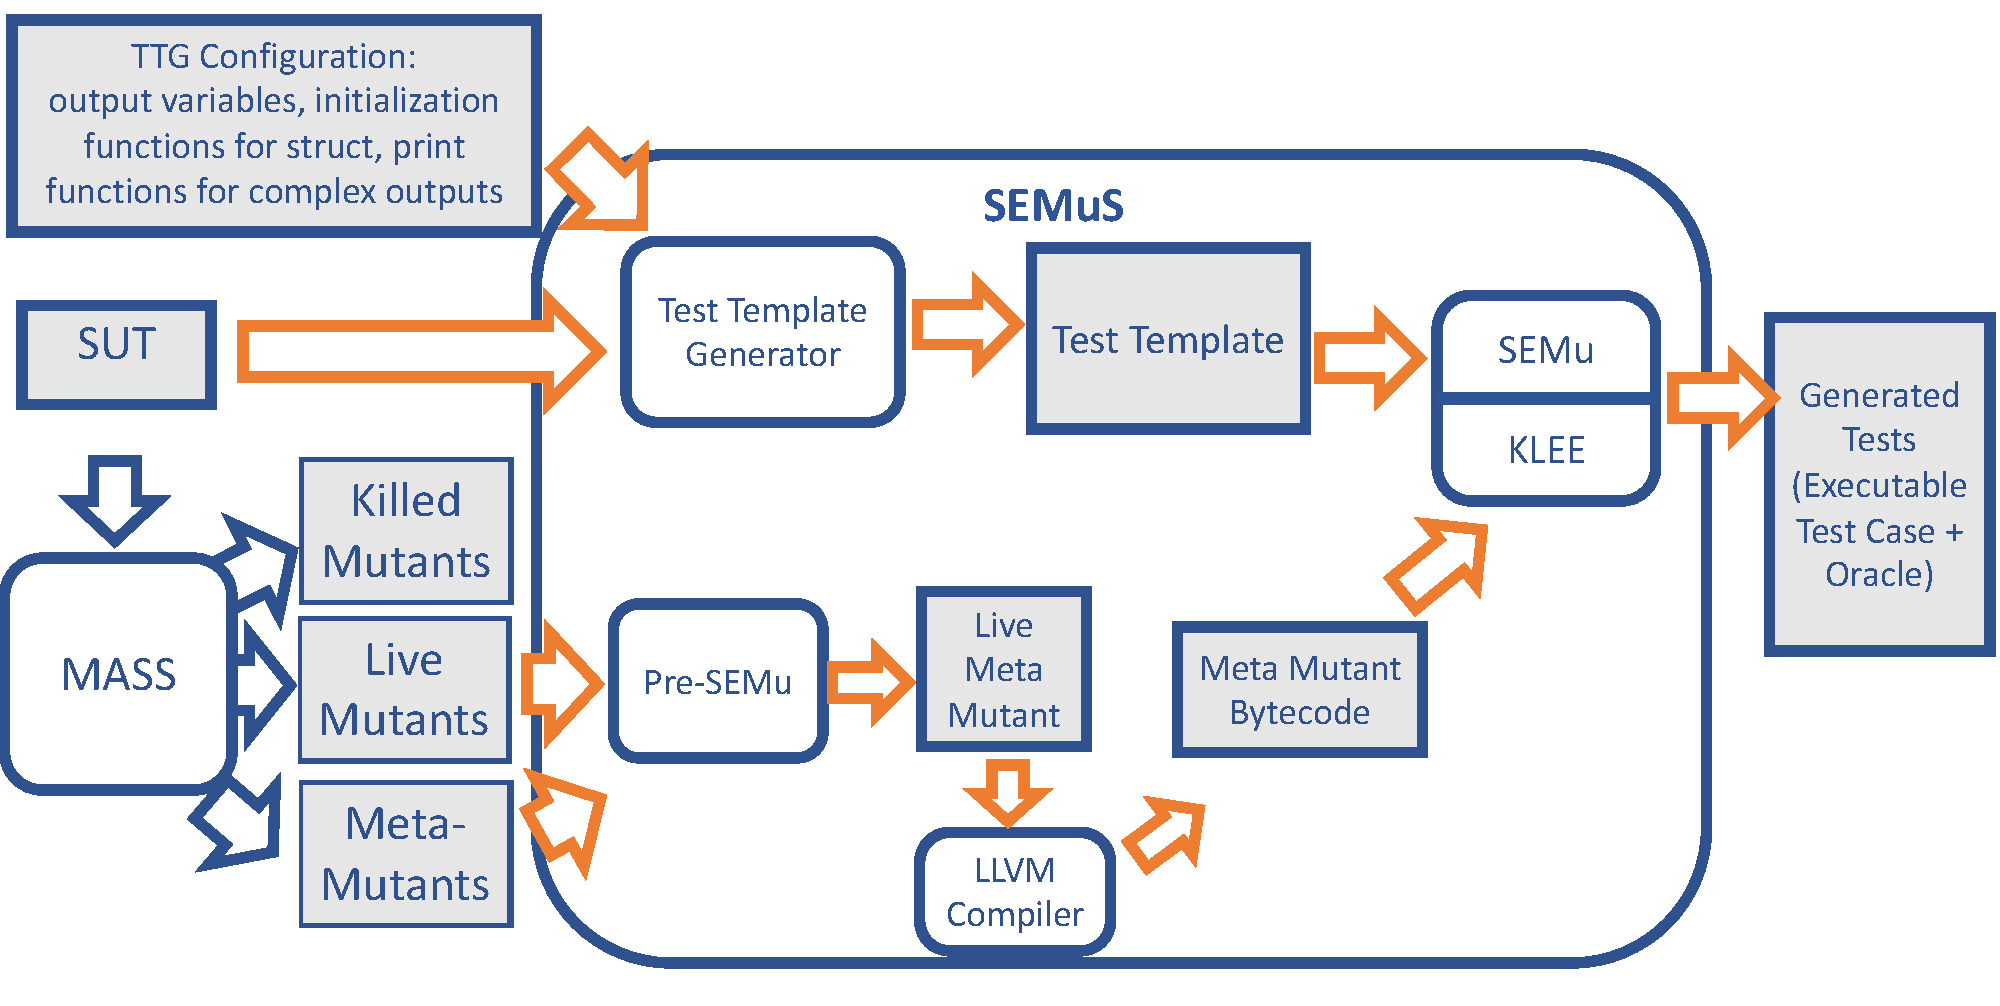
\includegraphics[width=0.8\textwidth]{images/semus-architecture2}
\caption{FAQAS-SEMuS Architecture and Workflow}
\label{fig:semus_architecture}
\end{center}
\end{figure}

%enable the adoption of SEMu in the space context. In particular, SEMuS (1) automates the generation of a test template including symbolic variables that guides the generation of test inputs, and (2) compiles the test template and the mutant into the format required by SEMu (i.e., LLVM-IR). 

\subsection{Test Template Generator}

The \INDEX{Test Template Generator} (TTG) component automates the generation of templates for the symbolic execution search. The component receives as inputs the SUT source code and the list of SUT functions. 

Listing~\ref{test_template} shows an example of a test template generated by the TTG. The TTG generates a template for every SUT function. The TTG parses the function arguments and declares them symbolic through use of the KLEE function \texttt{klee\_make\_symbolic}. Then, it adds a call to the function under analysis with symbolic values, and it saves the return value into a support variable (i.e., \texttt{result\_faqas\_semu} in Listing~\ref{test_template}). Finally, it generates a number of invocations of the \emph{printf} function that print the value of the software outputs and adds a return statement with the value returned by the function under test (e.g., \texttt{result\_faqas\_semu} in Listing~\ref{test_template}). 
Such \emph{printf} invocations are necessary because of the way SEMu determines that a mutant is killed; two are the cases in which the mutant is considered killed: (1) the main function returns a different return value, (2) different values are printed to the standard output. Consequently, it is necessary to print out all the values of the software outputs.
To select which variables to print, for every source file under test, the engineer can specify, in the SEMuS configuration file, the arguments (typically pointers) that should be either considered output or considered both input and outputs. By default, the TTG considers all the function arguments as inputs, in case some argument (e.g., a pointer to a memory buffer) is used both as input and as output the engineer shall specify it as such; similarly, in case some some argument (e.g., a pointer to a struct) is used to store outputs, the engineer shall indicate that it is an output. Moreover, since, in  the C language, the function \emph{printf} cannot automatically determine how to print the different fields specified in a data structure (i.e., it prints only the memory address of the pointer), the engineer can also specify how to printout the different fields of a data structure.

Listing~\ref{test_config} shows an example configuration file for SEMuS. In addition to output arguments (i.e., \emph{OUT\_\-ARGS\_NAMES}), input/output arguments (i.e., \emph{IN\_OUT\_ARGS\_NAMES}), and customized printf instructions (i.e., \emph{TYPES\_TO\_PRINTCODE}), the SEMuS configuration file enables the engineer to customize the generation of the test template further. Indeed, engineers can specify input argument types that should not be treated symbolically but that shall be initialized using a specific function of the SUT (i.e., \emph{TYPE\_TO\_INITIALIZATION\-CODE}); also, engineers can specify the fields, within such types (e.g., the attributes of a struct), that shall be treated symbolically.
Moreover, since the template returns the value of the function under test, the engineer can specify how to convert the returned value to int, if necessary (see parameter \emph{TYPES\_TO\_INTCONVERT}). Finally, in case the function under test receives a pointer to an array (which is typically passed as a pointer), the engineer can specify the size of such array (see parameter \emph{ARG\_TYPE\_TO\_ITS\_POINTER\_ELEM\_NUM}); by default, SEMuS assumes that a pointer refers to a single element (i.e., it is a pointer to a variable not an array).  


% !TEX root =  ../MAIN.tex

\begin{lstlisting}[style=CStyle, caption=SEMuS test template., label=test_template]
int main(int argc, char** argv) {
    // Declare variable to hold function returned value
    _Bool result_faqas_semu; 
    // Declare arguments and make input ones symbolic
    unsigned long pVal;
    int pErrCode;
    klee_make_symbolic(&pVal, sizeof(pVal), "pVal"); // Call function under test
    result_faqas_semu = T_INT_IsConstraintValid(&pVal, &pErrCode); // Make some output
    printf("FAQAS-SEMU-TEST_OUTPUT: %d\n", pErrCode);
    printf("FAQAS-SEMU-TEST_OUTPUT: %d\n", result_faqas_semu);
    return (int)result_faqas_semu;
}

\end{lstlisting}


\begin{lstlisting}[language={}, caption=Klee-test output, label=ktest]
ktest file : 'test000001.ktest'
args       : ['/MakeSym-TestGen-Input/direct/T_INT_IsConstraintValid/test.MetaMu.bc']
num objects: 2
object    0: name: b'model_version'
object    0: size: 4
object    0: data: b'\x01\x00\x00\x00'
object    1: name: b'pVal'
object    1: size: 8
object    1: data: b'\x00\x00\x00\x00\x00\x00\x00\x00'
\end{lstlisting}

% !TEX root =  ../MAIN.tex

\begin{lstlisting}[float=h, style=CStyle, caption=SEMuS configuration example., label=test_config]
{
"TYPES_TO_INTCONVERT": {},
"TYPES_TO_PRINTCODE": {"gs_timestamp_t": "printf(\"FAQAS-SEMU-TEST-OUTPUT: result_faqas_semu = tv_sec: %u, tv_nsec: %u\\n\", {}.tv_sec, {}.tv_nsec);"},
"OUT_ARGS_NAMES": ["pErrCode"],
"IN_OUT_ARGS_NAMES": ["base"],
"TYPE_TO_INITIALIZATIONCODE": {},
"TYPE_TO_SYMBOLIC_FIELDS_ACCESS": {},
"VOID_ARG_SUBSTITUTE_TYPE": "",
"ARG_TYPE_TO_ITS_POINTER_ELEM_NUM": {"char *": 6}
}
\end{lstlisting}


\subsection{Pre-SEMu}

The \INDEX{Pre-SEMu} component generates \INDEX{mutant schemata}; specifically, the component includes and compiles all the live mutants (i.e., MASS output) into a single bytecode file named the \emph{Meta Mutant}. SEMu will select which mutant to consider for test generation based on a parameter. The compilation of the Meta Mutant into LLVM bitcode is supported by the \emph{LLVM} compiler infrastructure. 

% !TEX root =  ../MAIN.tex



\begin{lstlisting}[style=CStyle, float=h, caption=Function T\_INT\_IsConstraintValid., label=original_meta]
flag T_INT_IsConstraintValid(const T_INT* pVal, int* pErrCode)
{
    flag ret = TRUE;
    (void)pVal;

    ret = ((*(pVal)) <= 50UL);
    *pErrCode = ret ? 0 :  ERR_T_INT;

    return ret;
}
\end{lstlisting}

\begin{lstlisting}[style=CStyle, float=h, caption=Mutant 1 of function T\_INT\_IsConstraintValid., label=meta_mutant_1]
flag T_INT_IsConstraintValid(const T_INT* pVal, int* pErrCode)
{
    flag ret = TRUE;
    (void)pVal;

    ret = ((*(pVal)) <= 50UL);
    *pErrCode = ret ? 1 :  ERR_T_INT;

    return ret;
}
\end{lstlisting}

\begin{lstlisting}[style=CStyle, float=h, caption=Mutant 2 of function T\_INT\_IsConstraintValid., label=meta_mutant_2]
flag T_INT_IsConstraintValid(const T_INT* pVal, int* pErrCode)
{
    flag ret = TRUE;
    (void)pVal;

    ret = ((*(pVal)) <= 50UL);
    *pErrCode = ret ? (-1) :  ERR_T_INT;

    return ret;
}
\end{lstlisting}

\begin{lstlisting}[style=CStyle, float=h, caption=Meta-Mutant for function T\_INT\_IsConstraintValid., label=meta_mutant_example]
flag T_INT_IsConstraintValid(const T_INT* pVal, int* pErrCode)
{
    flag ret = TRUE;
    (void)pVal;

    ret = ((*(pVal)) <= 50UL);

    klee_semu_GenMu_Mutant_ID_Selector_Func(1,2);
    *pErrCode = ret ? 
    	( klee_semu_GenMu_Mutant_ID_Selector==2 ?
    		((-1)):
		    (klee_semu_GenMu_Mutant_ID_Selector==1?
			    (1):
			    (0))) 
			    :  ERR_T_INT;
    klee_semu_GenMu_Post_Mutation_Point_Func(0,0);
    klee_semu_GenMu_Post_Mutation_Point_Func(1,2);

    return ret;
}
\end{lstlisting}

Listings~\ref{original_meta} provides the source code of function \emph{T\_INT\_IsConstraintValid}, while Listings~\ref{meta_mutant_1} and~\ref{meta_mutant_2} provide two example mutants generated by MASS.
Listing~\ref{meta_mutant_example} provides an example \INDEX{meta-mutant} including the same two mutants of Listings~\ref{meta_mutant_1} and~\ref{meta_mutant_2}. 
To select the mutants to analyze at runtime, SEMu relies on three support functions that shall be invoked within the eta-mutant:

\begin{itemize}
	\item \texttt{klee\_semu\_GenMu\_Mutant\_ID\_Selector\_Func}: function that takes two mutant IDs as arguments, representing a range of mutant IDs. It specifies where a portion of code containing mutants start.
    \item \texttt{klee\_semu\_GenMu\_Mutant\_ID\_Selector}: global variable that contains the ID of the mutant to be activated durng the analysis with SEMu.
	\item \texttt{klee\_semu\_GenMu\_Post\_Mutation\_Poin\_Func}: 
	function that takes two mutant IDs as arguments, it specifies where a portion of code containing mutants ends.
	It is used by SEMu to identify the portion of the code where to compare the state of the original and the mutated program and determine if the mutation has affected the program state (i.e., the \INDEX{necessity} condition to kill a mutant). In other words, it enables SEMu to perform conservative pruning and remove the mutant states that are not infected.
\end{itemize}

In Listing~\ref{meta_mutant_example}, mutant 2 from Listing~\ref{meta_mutant_2} appears on line 11 (indeed, the value \emph{-1} is selected when the mutant ID is equal to 2). Mutant 1 from Listing~\ref{meta_mutant_1} appears on line 12 (indeed, the value \emph{1} is selected when the mutant ID is equal to 1). The original software is represented by the mutant ID zero; indeed the value \emph{0} (i.e., what appears in line 7 of the Listing~\ref{original_meta}) is selected on line 14 (i.e., when the mutant ID is neither \emph{2} nor \emph{1}).

\subsection{KLEE-SEMu}



\INDEX{KLEE-SEMu} is the underlying test generation component, previously described in Section~\ref{sec:testGen:CP}. This component receives as inputs the \emph{LLVM bitcode} of the \emph{Meta Mutant} and the \emph{Test Template} for the function under test, and proceeds to apply dynamic symbolic execution to generate test inputs to kill the mutants. The output of this component are the \emph{KLEE tests}.

% \TODO{you need to list what are "the parameters of the execution"}
A \INDEX{KLEE test} is a binary file that contains information about the execution of KLEE such as the entry point of the analysis, and the generated test inputs.


An example of a KLEE test is presented in Listing~\ref{ktest}. The field \emph{args} report the entry point of the analysis; in this case, the test generation was performed for live mutants present in the function \texttt{T\_INT\_Is\-Constraint\-Valid}, which SEMuS stores in a dedicated folder. The fields named \emph{object} provide information about the outputs generated by KLEE (e.g., the generated test inputs). 
For each object, the KLEE test provides a \emph{name} (usually the name of the symbolic variable), its \emph{size}, and the actual \emph{value} generated by KLEE through constraint solving (usually this is reported in binary form).
Objects are numbered. Object number \emph{0} reports information about the data structure used by KLEE, that is, the version of the structure. The other objects report information about the generated test inputs.
Our example shows that one value of size 8 was generated for the variable \texttt{pVal}, the data field shows the binary representation of the \texttt{pVal} variable, in this case \texttt{pVal=0}.

% !TEX root =  ../MAIN.tex
\begin{lstlisting}[float=t, language={}, caption=Klee-test output, label=ktest]
ktest file : 'test000001.ktest'
args       : ['/MakeSym-TestGen-Input/direct/T_INT_IsConstraintValid/test.MetaMu.bc']
num objects: 2
object    0: name: b'model_version'
object    0: size: 4
object    0: data: b'\x01\x00\x00\x00'
object    1: name: b'pVal'
object    1: size: 8
object    1: data: b'\x00\x00\x00\x00\x00\x00\x00\x00'
\end{lstlisting}

\subsection{KTest to Unit Test}

% !TEX root =  ../MAIN.tex

\begin{lstlisting}[float=t, style=CStyle,  caption=Generated test case, label=gen_test_case]
#include <stdio.h>
#include <string.h>

#include "asn1crt.c"
#include "asn1crt_encoding.c"
#include "asn1crt_encoding_uper.c"


int main(int argc, char** argv)
{
    (void)argc;
    (void)argv;

    // Declare variable to hold function returned value
    _Bool result_faqas_semu;

    // Declare arguments and make input ones symbolic
    unsigned long pVal;
    int pErrCode;
    memset(&pVal, 0, sizeof(pVal));
    const unsigned char pVal_faqas_semu_test_data[] = {0x00, 0x00, 0x00, 0x00, 0x00, 0x00, 0x00, 0x00};
    memcpy(&pVal, pVal_faqas_semu_test_data, sizeof(pVal)); // Unsigned val is 0

    // Call function under test
    result_faqas_semu = T_INT_IsConstraintValid(&pVal, &pErrCode);

    // Make some output
    printf("FAQAS-SEMU-TEST_OUTPUT: pErrCode = %d\n", pErrCode);
    printf("FAQAS-SEMU-TEST_OUTPUT: result_faqas_semu = %d\n", result_faqas_semu);
    return (int)result_faqas_semu;
}
\end{lstlisting}



The component \INDEX{KTest to Unit Test} (KTU) converts a KLEE test into a human readable, compilable, and executable C test case. The unit test case generated by KTU, match the test template generated by TTG except for the declaration of variables where symbolic variables are replaced with concrete variables initialized with the values stored in the KTest file.
 
Listing~\ref{gen_test_case} shows an example of a test case generated for a mutant present in the function \texttt{T\_INT\_Is\-ConstraintValid}. For instance, line 20 shows that the variable \texttt{pVal} is initially filled with zeros, then in line 21, it is filled with the value stored in the variable \texttt{pVal\_faqas\_semu\_test\_data}, which holds the binary output produced by KLEE. In line 25, the function under test is invoked with the concrete value of \texttt{pVal}. 

The test case generated by the KTU prints the function return value and the value of every variable passed by reference, using the same instructions of the test template.
KTU cannot generate test assertions because only engineers can know, based on specifications, what are the values to be expected at the end of the test case execution.
However, the generated printf invocations still play the role of an oracle for regression testing, as explained in the next sections.

\subsection{Test suite augmentation} 
\label{sec:Semus:augment}
The procedure for testing with SEMuS is shown in Figure~\ref{fig:semus:test:example}.
In Step 1, the engineer executes SEMuS, which generates an output folder for every live mutant that is killed by the generated test cases.
Every folder contains: a script (i.e., \emph{runTest.sh}) that can be used to execute the generated test case, (2) the test case itself (i.e., test1.c), and (3) a text file with extension \emph{.expected} that contains the output that is observed when executing the test case with the SUT.
In Step 2, the engineer visually inspects every file with extension \emph{.expected} to determine if the observed output matches the specifications; if not, the software is faulty and needs to be fixed. In this case mutation testing enables detecting a fault. 
After verifying all the generated files with extension \emph{.expected} the engineer can reuse the test cases generated by SEMuS for regression testing in future versions of the SUT. Basically, the output folders generated by SEMuS become part of the test suite of the SUT.

When there is a new version of the SUT (Step 3, in Figure~\ref{fig:semus:test:example}), the folder with the source code of the SUT is replaced with the new version of the SUT (this can be done automatically with version control software).
The engineer can then trigger test execution by simply re-executing all the scripts \emph{runTest.sh} generated by SEMuS.
The script \emph{runTest.sh} first executes the test case (Step 4.1), then it stores the test outputs into a text file with extension \emph{.got}, finally if compares the observed output with the output generated for the previous version. If the function under test was not modified, differences may indicate that the test case FAILED.

\begin{figure}[h]
\begin{center}
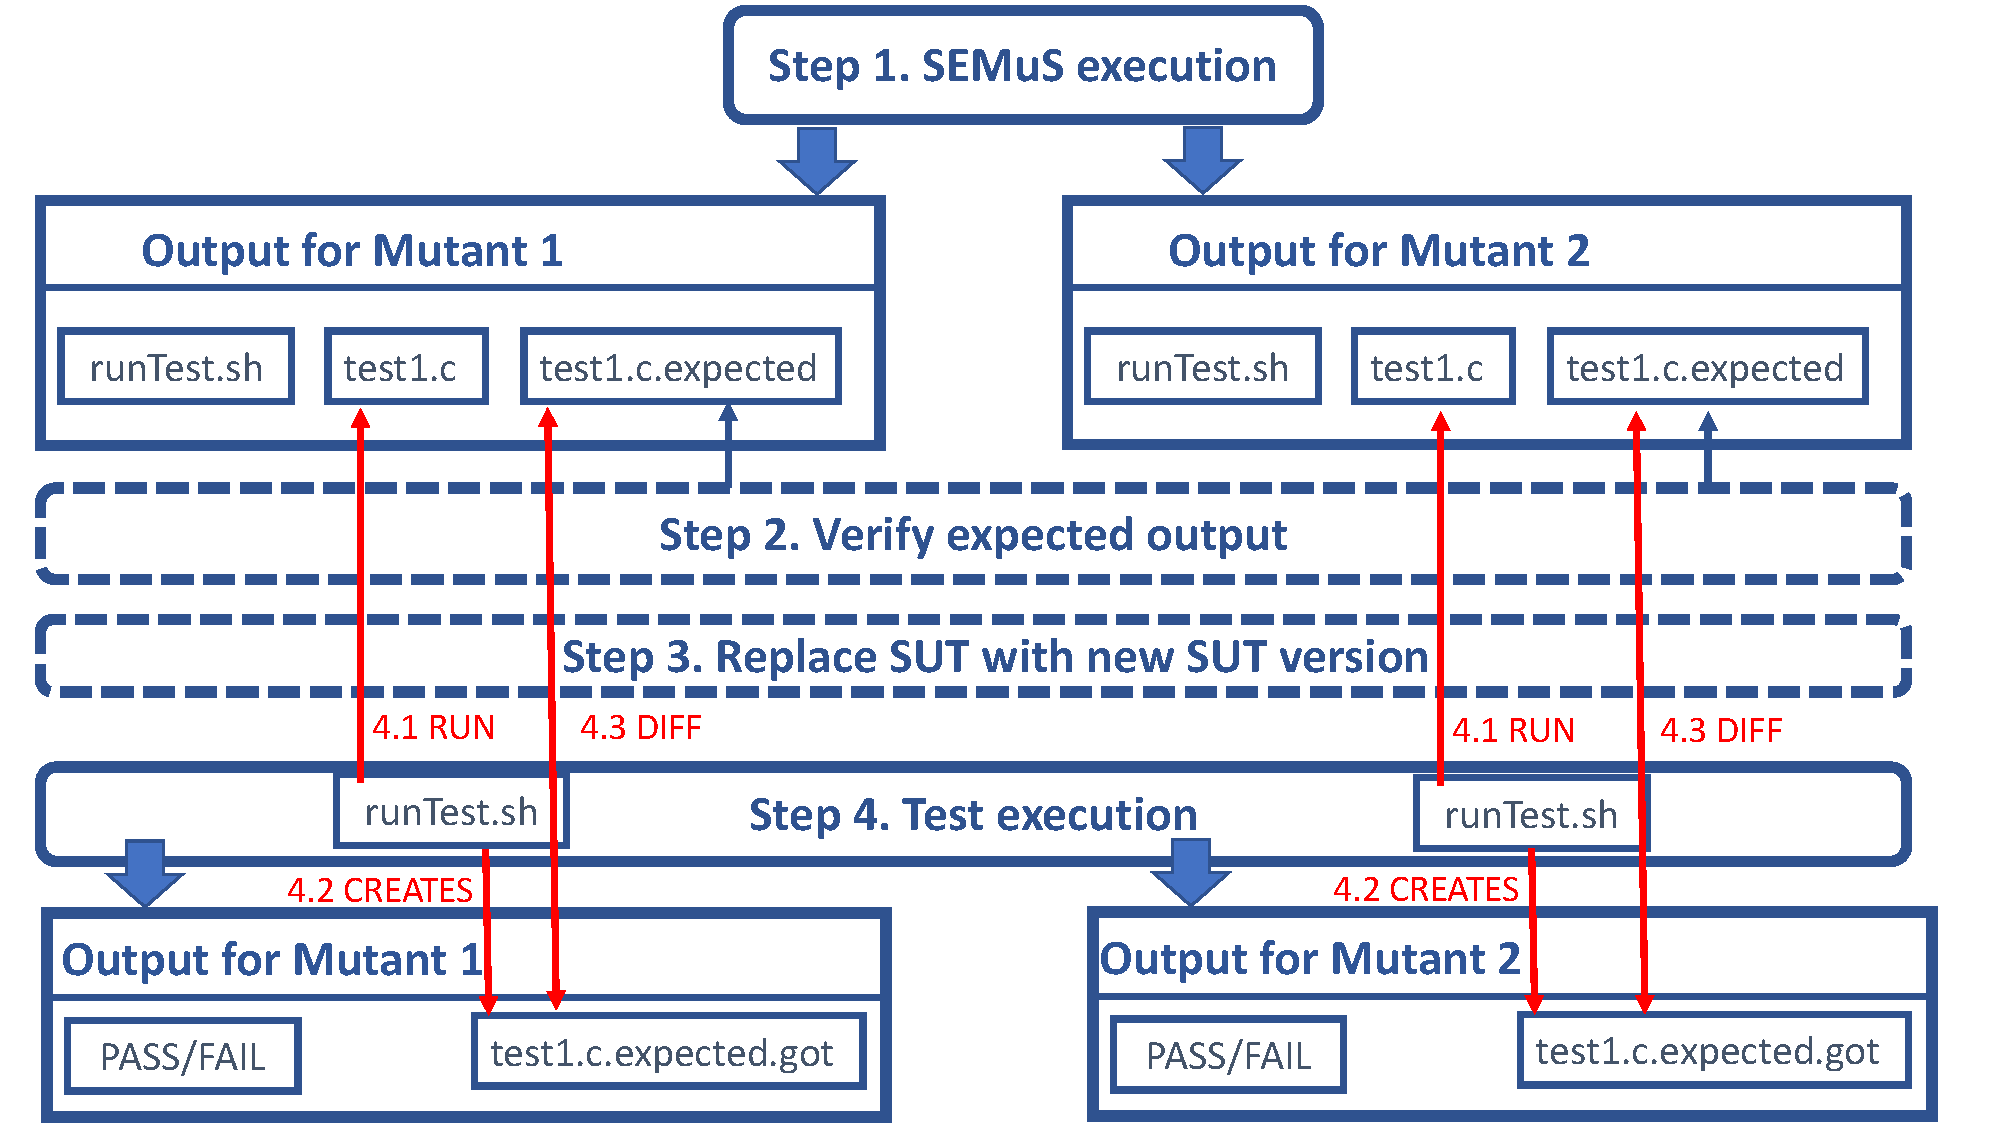
\includegraphics[width=0.8\textwidth]{images/semus-out}
\caption{Workflow for test suite augmentation with SEMuS}
\label{fig:semus:test:example}
\end{center}
\end{figure}

\subsection{Live mutants}

SEMuS may not be capable of selecting test inputs that kill the mutant under analysis. We may distinguish two cases:
\begin{itemize}
\item SEMuS execution terminates and no test case is generated.
\item SEMuS execution does terminate (i.e., it is killed after a timeout configured by the end-user, usually 15 minutes are sufficient to generate test cases).
\end{itemize}

In the first case, SEMuS has successfully exercised all the execution paths covering the mutated statements but did not identify inputs that satisfy the killing conditions. This may case indicate that the mutant is equivalent and may be discarded (however, the engineer shall verify that the test template is configured correctly). Also, we may be in such situations when some of the functions under test belong to libraries not compiled with LLVM that, consequently are not correctly processed by KLEE-SEMu; to detect these cases the engineer shall look for errors in the output generated by KLEE.

In the second case, SEMuS did not complete the analysis of the possible execution paths covering the mutated statement. Such cases may indicate that test generation is complex and probably an engineer may more efficiently select test inputs than the underlying constraint solving solution implemented by KLEE-SEMu.

% !TEX root =  ../MAIN.tex
\clearpage
\section{Data-driven Mutation Analysis: DAMAt}

\renewcommand{\APPR}{DAMAt\xspace{} }


\subsection{Overview}

In this Section, we propose \INDEX{data-driven mutation analysis}, 
a new mutation analysis paradigm
that alters the data exchanged by software components to evaluate the capability of a test suite to detect interoperability faults. Also, we present a technique, \INDEX{data-driven mutation analysis with tables} (\APPR),
to automate data-driven mutation analysis by relying on
a fault model that captures, for a specific set of components, both the characteristics of the data to mutate (e.g., the size and structure of the messages generated by the ADCS) and the types of fault that may affect such data (e.g., a  value out of the nominal range). The latter is formalized as a set of parameterizable mutation operators. 
To simplify adoption, we rely on fault models in tabular form where each row specifies, for a given data item, what mutation operator (along with its corresponding parameter values) to apply to which elements of the data item.
At runtime, \APPR modifies the data exchanged by components according to the provided fault model (e.g., replaces a nominal voltage value with a value out of the nominal range).






\INDEX{Data-driven mutation analysis} aims to evaluate the effectiveness of a test suite in detecting \INDEX{semantic interoperability \UPDATED{faults}}. 
It is achieved by modifying (i.e., mutating) the data exchanged by CPS components. It generates \INDEX{mutated data} that is representative of data that might be observed at runtime in the presence of a component that behaves differently than expected in the test case; also, it mutates  data that is not automatically corrected by the software 
(e.g., through cyclic redundancy check codes)
%(e.g., through CRC mechanisms, which aim to correct technical interoperability problems) 
and thus causes software failures (i.e., the mutated data shall have a different semantic than the original data). For these reasons, data mutation is driven by a fault model specified by the engineers based on domain knowledge.

Although different types of fault models might be envisioned,
%see background
we propose a technique (\INDEX{data-driven mutation analysis with tables}, \APPR),
which automates data-driven mutation analysis by relying on
a tabular \CHANGED{block model}, itself tailored to the \UPDATED{SUT} through predefined mutation operators.
To concretely perform data mutation at runtime, \APPR relies on a set of \INDEX{mutation probes} that shall be integrated by software engineers into the software layer that handles the communication between components. The runtime behaviour of mutation probes (i.e, what data shall be mutated and how) is driven by the fault model. Thus, \APPR can automatically generate the implementation of mutation probes from the provided fault model.
Depending on the CPS, probes might be inserted either into the \UPDATED{SUT}, into the simulator infrastructure, or both.
For example, Figure~\ref{fig:appr:mutateProbesInserted} shows the architecture of the \ESAIL satellite system with mutation probes integrated into the SVF
%\footnote{Software Validation Facility~\cite{Isasi2019}; it usually includes one or more simulators, an emulator to run the code compiled for the target hardware, and test harnesses.} 
functions that handle communication with external components (PDHU, GPS, and ADCS in this case). 






\APPR works in six steps, which are shown in Figure~\ref{fig:appr:approach}. 
In Step 1, based on the provided methodology and predefined mutation operators, the engineer prepares a fault model specification tailored to the SUT.
% capturing the data format and the types of faults that shall be injected for every data item exchanged by the system components.
In Step 2, \APPR generates a mutation API with the functions that modify the data according to the provided fault model.
In Step 3, the engineer modifies the \UPDATED{SUT} by introducing mutation probes (i.e., invocations to the mutation API) into it.
\REVTOOL{P-2}{Instead of modifying the SUT the engineer may modify the test harness (e.g., the SVF simulator); such choice depends on the software under test, if the test cases are executed through a simulator, such choice prevents introducing damaging changes into the SUT (e.g., delay task execution and break strict real-time requirements).}
In Step 4, \APPR generates and compiles mutants. 
Since the \APPR mutation operators may generate mutated data by applying multiple mutation procedures, \APPR may generate several mutants, one for each \UPDATED{mutation operation (i.e., a mutation procedure configured for a data item, according to our terminology, see Section~\ref{sec:mutantsGeneration})}.
In Step 5, \APPR executes the test suite with all the mutants including a mutant (i.e., the coverage mutant) which does not  modify the data but traces the coverage of the fault model.
In Step 6, \APPR generates mutation analysis results.

%\UPDATED{
%In our context, the \emph{software under test (SUT)} is the CPS embedded software that is verified by a test suite, which is the target of data-driven mutation analysis. Therefore, we refer to the software developed by the engineers as the \emph{original SUT}. An \emph{SUT mutant} (simply, a \emph{mutant}) is a version of the SUT that integrates a \emph{mutation probe} and shall make test cases fail. 
%%A mutation operator simulates one specific interoperability error (a specific type of that automatically alters data by applying one specific \emph{mutation operation}.
%}

In the following sections we describe the structure of our fault model and each step of \APPR.

\begin{figure}[h]
	\centering
		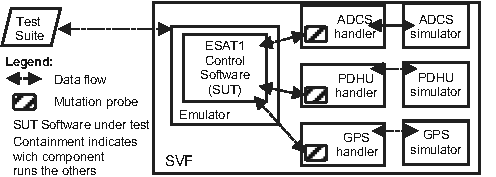
\includegraphics[width=8.4cm]{damat/images/dataMutationExample}
		\caption{\CHANGED{Data mutation probes integrated into \ESAIL.}}
		\label{fig:appr:mutateProbesInserted}
	\end{figure}

\begin{figure}[h]
	\centering
		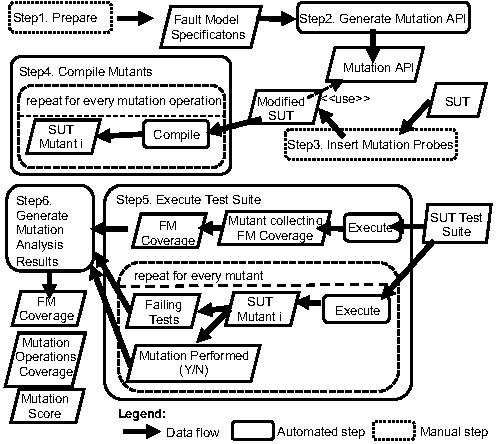
\includegraphics[width=8cm]{damat/images/dataDrivenBufferProcess}
		\caption{The \APPR process.}
		\label{fig:appr:approach}
	\end{figure}


\subsubsection{Fault Model Structure}
\label{sec:faultModelStructure}





The \APPR fault model enables the specification of the format of the data exchanged between components along with the type of faults that may affect such data. 
In this paper, we refer to the data exchanged by two components as \INDEX{message}; also, each CPS component may generate or receive different \INDEX{message types}.
For a single CPS, more than one fault model can be specified. For example, in the case of \ESAIL{} we have defined one fault model for every message type that could be exchanged by the three components under test (i.e., ADCS, PDHU, and GPS). In total, for \ESAIL, we have 14 fault models, 10 for the communication concerning ADCS (we have 10 different message types), 3 for PDHU, and 1 for GPS.

The \APPR fault model enables the modelling of data that is exchanged through a specific data structure: the data buffer. This was decided because it is a simple and widely adopted data structure for data exchanges between components in CPS. Also, more complex data structures (e.g., hierarchical ones like trees) are often flattened into data buffers in order to be exchanged by different components (e.g., through the network). When the CPS software is implemented in C or C++ (common CPS development languages) data buffers are implemented as arrays. Figure~\ref{fig:appr:bufferStructure} shows three block diagrams representing (part of) the buffer structure used to exchange messages of type InterfaceHouseKeeping and InterfaceStatus in \ESAIL.

A data buffer is characterized by a \INDEX{unit size} that specifies the dimension, in bytes, of the single cell of the underlying array and a \INDEX{buffer size}, which specifies the total number of units belonging to the buffer. Each data buffer can contain one or more \INDEX{data items}; the size of data items may vary as they may span over multiple units. Also, each data item is interpreted by the CPS software according to a specific \INDEX{representation} (e.g., integer, double, etc.). 
In \ESAIL, the unit size is one byte and the data items may span over one or two buffer units (see Figure~\ref{fig:appr:bufferStructure}). 
%Figure~\ref{} provides an example buffer instance for a \emph{Magnetorquer Set PWM RSP message}.

The \APPR fault model enables engineers to specify (1) the \emph{position} of each data item in the buffer, (2) their \emph{span}, and (3) their \emph{representation type}. Our current implementation supports six data representation types: int, long int, float, double, bin (i.e., data that should be treated in its binary form), hex (i.e., data that should be treated as hexadecimal).
Further, for each data item, \APPR enables engineers to specify one or more data faults using the mutation operator identifiers. For each operator, the engineer 
shall provide values for the required configuration parameters.

Table~\ref{table:operators} provides the list of mutation operators included in \APPR along with their description. The \APPR mutation operators generate \INDEX{mutated data item instances} through one or more \INDEX{mutation procedures}, which are the functions that generate a mutated data item instance given a correct data item instance observed at runtime. For example, the \emph{VAT} operator includes only one mutation procedure (i.e., setting the current value above the threshold) while the \emph{VOR} operator includes two mutation procedures, which are
(1) replacing the current value with a value above the specified valid range and (2) replacing the current value with a value below the valid range.
The operators VOR, BF, INV, and SS have been inspired by related work~\cite{di2015generating,PeachFuzzer,Matinnejad19}; the operators VAT, VBT, FVAT, FVBT, FVOR, IV, ASA,  and HV
are a contribution of this paper and were derived and conceptualised as a result of discussion with domain experts.
Although other data representation types (e.g., null terminated strings) and operators (e.g., replacement of a random char in a string) might be envisioned, in this paper, we focus on operators that are necessary in the CPS context, based on our experience.
For example, CPS components are unlikely to exchange strings.
%are a contribution of this paper, based on discussion with domain experts. 

\begin{figure}
	\centering
		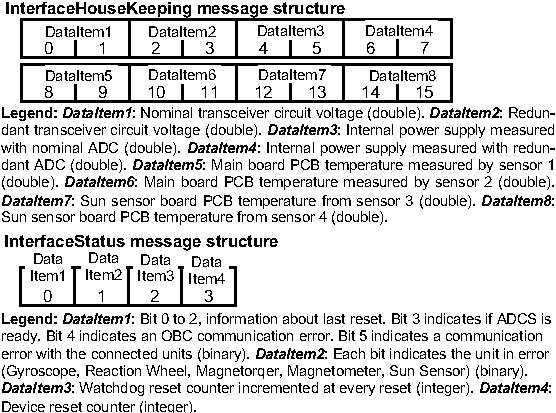
\includegraphics[width=8.4cm]{damat/images/BufferStructuresSmall}
		\caption{Structure of data buffers in \ESAIL.}
		\label{fig:appr:bufferStructure}
	\end{figure}
	
	% !TEX root = ../MAIN-DataDrivenMutationAnalysis.tex


\begin{table*}[tb]
\caption{Data-driven mutation operators}
\label{table:operators}
\scriptsize
\begin{tabular}{|p{40mm}|p{90mm}|}
\hline
\textbf{Fault Class}&\textbf{Description}\\
\hline
Value above threshold (VAT)&
Replaces the current value with a value above the threshold T for a delta (\D). 
\\
\hline
Value below threshold (VBT)&
Replaces the current value with a value below the threshold T for a delta (\D). 
\\
\hline
Value out of range (VOR)&
Replaces the current value with a value out of the range $[MIN;MAX]$.\\
\hline
Bit flip (BF)&
A number of bits randomly chosen in the positions between MIN and MAX are flipped.
\\
\hline
Invalid numeric value (INV)&
Replace the current value with a mutated value that is legal (i.e., in the specified range) but different than current value. 
\\
\hline
Illegal Value (IV)
&
Replace the current value with a value that is equal to the parameter \emph{VALUE}. 
\\
\hline
Anomalous Signal Amplitude (ASA)
&
The mutated value is derived by amplifying the observed value by a factor \emph{V} and by adding/removing a constant value \D from it. 
\\
\hline
Signal Shift (SS)
&
The mutated value is derived by adding a value \D to the observed value. 
\\
\hline
Hold Value (HV)
&
This operator keeps repeating an observed value for $V$ times. It emulates a constant signal replacing a signal supposed to vary.
\\
\hline
Fix value above threshold (FVAT)&
In the presence of a value above the threshold, it replaces the current value with a value below the threshold T for a delta \D. 
\\
\hline
Fix value below threshold (FVBT)&
It is the counterpart of FVAT for the operator VBT.
\\
\hline
Fix value out of range (FVOR)&
In the presence of a value out of the range  $[MIN;MAX]$ it replaces the current value with a random value within the range. 
\\
\hline
\end{tabular}
\end{table*}%

\clearpage

%\begin{figure}
%	\centering
%		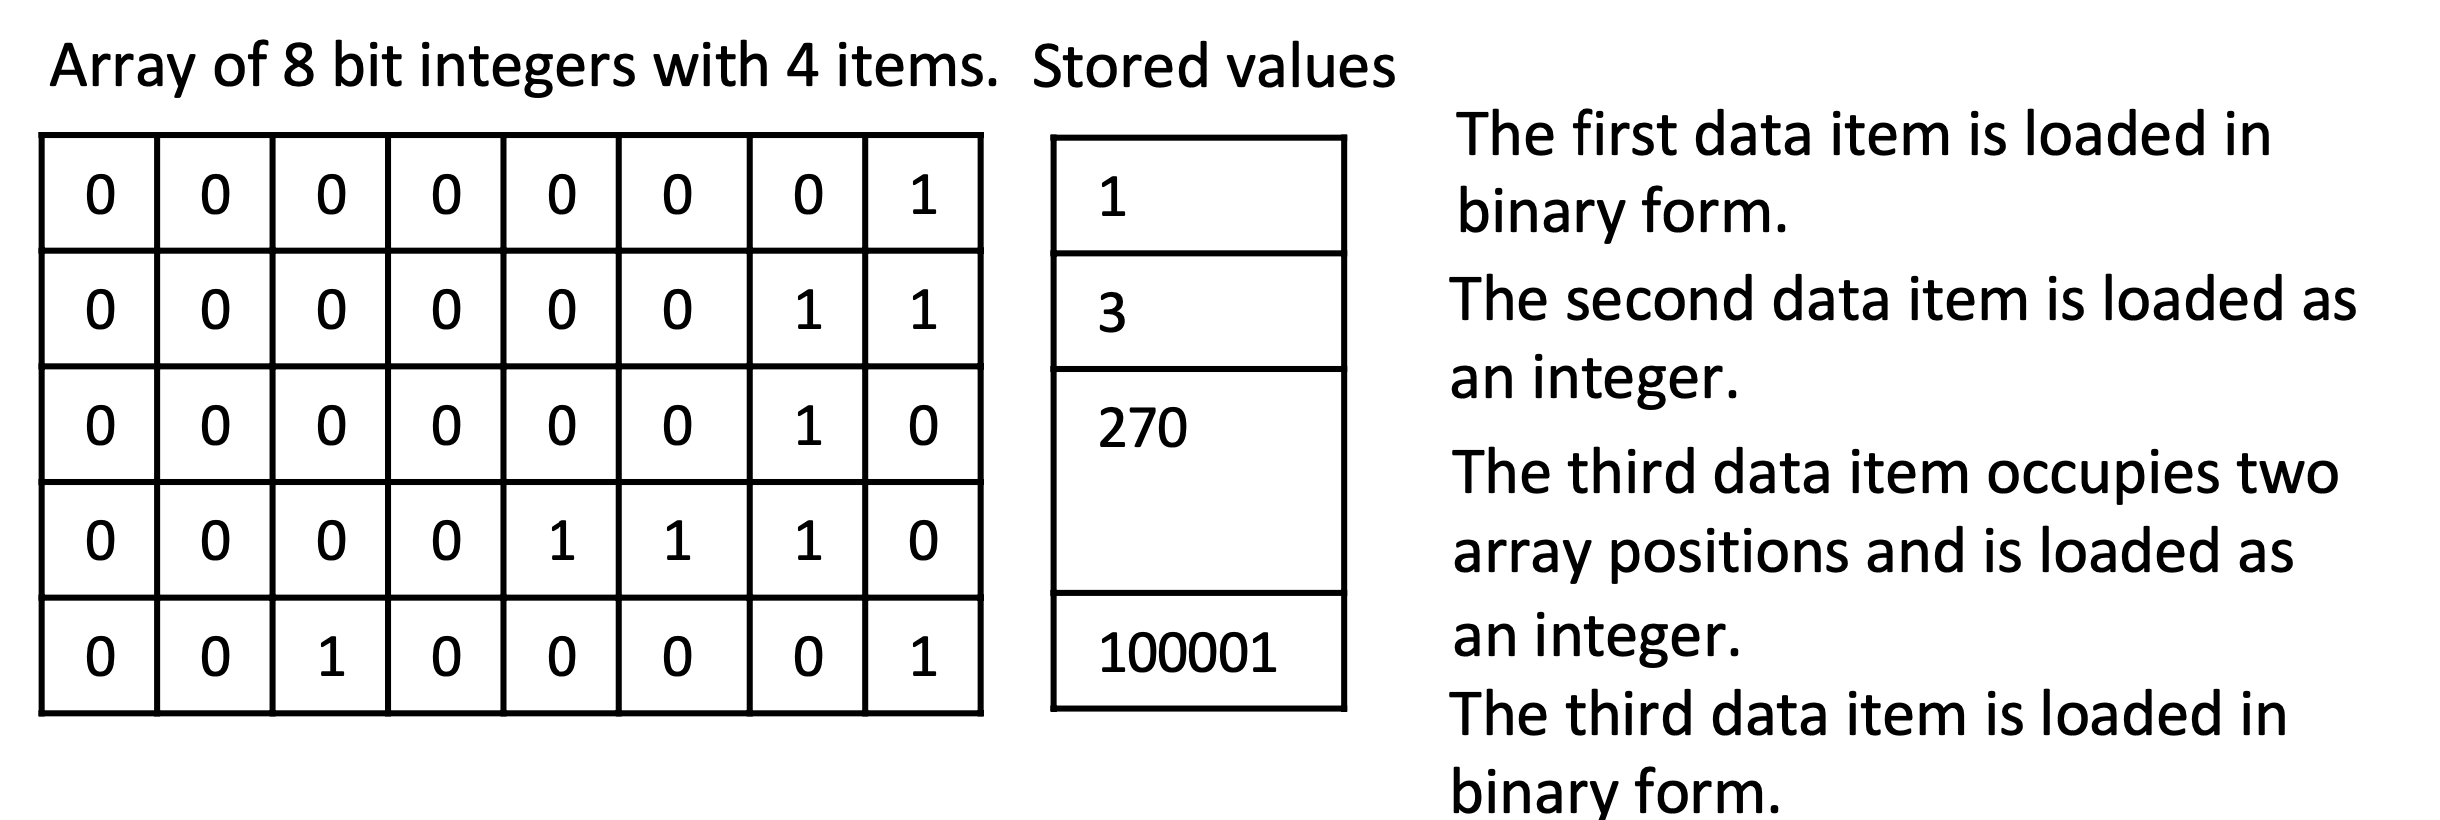
\includegraphics[width=8cm]{damat/images/bufferExample}
%		\caption{Example of a data buffer. \TODO{UPDATE PICTURE}}
%		\label{fig:appr:buffer}
%	\end{figure}

\subsubsection{Fault Modelling Methodology (Step 1)}
\label{sec:methodology}

% !TEX root =  ../MAIN-DataDrivenMutationAnalysis.tex

%
%\setlength\LTleft{0pt}
%\setlength\LTright{0pt}
%\begin{longtable}{@{\extracolsep{\fill}}|p{2.5cm}|p{5cm}|p{5cm}|@{}}
%\toprule


\begin{table}[tb]
\caption{\APPR fault modelling methodology}
\label{table:method}
\center
\scriptsize
\begin{tabular}{|
@{\hspace{1pt}}>{\raggedleft\arraybackslash}p{10mm}@{\hspace{1pt}}|
@{\hspace{1pt}}>{\raggedleft\arraybackslash}p{15mm}@{\hspace{1pt}}|
@{\hspace{1pt}}>{\raggedleft\arraybackslash}p{15mm}@{\hspace{1pt}}|
@{\hspace{1pt}}>{\raggedleft\arraybackslash}p{10mm}@{\hspace{1pt}}|
@{\hspace{1pt}}>{\raggedleft\arraybackslash}p{13mm}@{\hspace{1pt}}|
@{\hspace{1pt}}>{\raggedleft\arraybackslash}p{17mm}@{\hspace{1pt}}|
}
\hline
\textbf{Data} \textbf{nature}&\textbf{Representation} \textbf{type}&\textbf{Dependencies}&\textbf{\# of input} \textbf{partitions}&\textbf{Operators}&\textbf{Comments}\\
\hline
numerical&I, L, F, D&stateless/stateful&2&[VAT,FVAT]&Nominal below T\\
&&&&or [VBT,FVBT]&Nominal above T\\
\cline{4-6}
&&&3 or more&[VOR,FVOR]&\\
\cline{3-6}
&&stateful&&INV&For valid range\\
\cline{4-6}
&& &&[VOR,FVOR]&For out of range\\
\cline{3-6}
&&signal&&ASA, SS, HV&\\
\hline
categorical&I, H&N/A&N/A&IV&\\
\cline{2-6}
%&string&N/A&N/A&BF\\
%\cline{2-5}
&B&N/A&N/A&BF&\\
\hline
ordinal&I, H&N/A&N/A&ASA&\\
\hline
other&B&N/A&N/A&BF&\\
\hline
\end{tabular}\\
\textbf{Legend:} N/A not applicable.
\end{table}
%\normalsize

The fault model shall enable the specification of 
all possible interoperability problems in the SUT while minimizing equivalent and redundant mutants.
Equivalent mutants have the same observable output as the original SUT. 
Instead, redundant mutants have the same observable output as other mutants.
We use the term \INDEX{observable output} to refer to any output that can be verified by the test suite.
The equivalent or redundant nature of a mutant depends
on the equivalence relation for observable outputs
(i.e., how to determine if two outputs are the same).
In a testing context, such equivalence relation depends on the type of testing being performed. For example, system test cases, different than unit test cases,  are unlikely to verify the values of all the state variables of the system and thus mutants that are nonequivalent for unit test suites might be considered equivalent for system test suites. 
For example, in satellite systems, the correctness of the GPS triangulation algorithm output is verified by unit test cases; system test cases, instead, verify 
if the software takes appropriate actions when the satellite is out of orbit. Consequently, slight changes in the coordinates communicated by the GPS component may not lead to any change in the observable output verified by the test suite.
%When defining a fault model, engineers shall thus select and configure mutation operators in such a way that the mutations performed trigger changes in the observable output of the SUT (to avoid equivalent mutants) and (2) distinct mutations do not lead to the same observable outputs (to avoid redundant mutants).


We provide a set of guidelines for the definition of fault models that 
are summarized in Table~\ref{table:method}. 
For guidance,
% are based on the characteristics of the data being exchanged by CPS components.
we account for the nature of the data (i.e., numerical, categorical, ordinal, or binary) and their representation type.
Also, for numerical data, 
we consider 
%the type of measurement, that is, if the data is counted (i.e., it is discrete) or measured (i.e., it is continuous) and
%For numerical data, mutations shall be defined taking into consideration
the data dependencies, that is how data values depend on the previously observed values; we identified three categories: stateless (i.e., there are no dependencies between consecutive values), stateful (i.e, values depend on previous ones), and signal (i.e., values derive from a function of independent variables like time).
\CHANGED{Data dependencies determine the granularity of the mutation (i.e., with data dependencies, small differences shall be noticed); for non numerical data, we do not provide mutation operators with different granularities and data dependencies can be ignored.}
%on previous values and the time in which they are observed).

 

For \INDEX{stateless numerical data}, our guidelines are driven by input space partitioning concepts~\cite{Ammann:Offutt:2008}.
Indeed, given equivalence relations among outputs, it is unlikely that every change in \INDEX{stateless numerical data} will result into nonequivalent mutants; however, we can partition the input domain into regions with equivalent values (partitions).
Precisely, we rely on the  
\INDEX{interface-based input domain modeling} approach~\cite{Ammann:Offutt:2008}:
%Within data-driven mutation analysis, 
for each data item we identify a number of input partitions (set of values or value ranges) according to the interface specifications of the interacting components.
%each data item represents an input partition that shall be split into sets of values (or value ranges) identified according to the interface specifications of the interacting components.
%an input partition corresponds to a single data item and it shall be split into a set of blocks defined according to the interface specifications of the interacting components. 
In our methodology, the number and type of mutation operators selected for stateless numerical data depend on the number of input partitions identified.
With \emph{two input partitions} (e.g., nominal and exceptional data values), engineers can rely either on the pair [VBT,FVBT] or the pair [VAT,FVAT]. 
%Engineers shall select the pair of operators that simplifies the reading of the fault model.
%FABRIZIO: initially, I have explained what I mean with simplyfiy the reading (see below), however, these are details that may not be that necessary in a 10 pages conference paper.
%Engineers shall select the pair of operators that simplifies the reading of the data model; precisely, when the two input partitions capture  ranges for nominal and exceptional data values, the selection depends on how exceptional cases are identified (i.e., below or above the threshold). For other cases (i.e., two input partitions not related to exceptional cases), engineers can select any of the two pairs.
With \emph{three partitions}, engineers must configure one VOR and one FVOR operator. If a different delta (\D) is considered for the upper and lower bounds, engineers may configure two pairs [VBT,FVBT] and [VAT,FVAT], for the lower and upper bound, respectively. In the presence of \emph{more than three} partitions, engineers shall configure one [VOR,FVOR] pair for each extra partition above three (e.g., two pairs in the case of five partitions). The parameter \D{} is used to determine the partition to which the mutated data belongs. 
%Please note that mutants belonging to each pair shall not lead to redundant mutants.
%Engineers can configure multiple [VOR,FVOR] pairs in case several combinations needs to be tested.


In the presence of \INDEX{stateful data}, replacement with random values in the valid range (i.e., the INV operator) will lead to nonequivalent mutants (e.g., because it leads to data values that are systematically different than the values expected for the current system state). Alternatively, the valid data range might be partitioned as for stateless data. However, to avoid redundant mutants, engineers should rely either on the INV operator or the partitioning of the valid data range. 
The effect of data outside the valid data range should instead be verified by means of the [VOR, FVOR] pair.

For \INDEX{signal values}, depending on the shape of the expected signal, engineers should configure one operator among the ASA, SS, and HV. The configuration of more than one of these operators may lead to redundant mutants (e.g., because each of them triggers the same warning in the SUT).

With \INDEX{categorical data} represented using \emph{integers and hexadecimals}, engineers must configure one IV operator for each possible value; indeed, a change in the observed category shall trigger a different behaviour in the SUT. 
%With categorical data represented using labels (e.g., strings), engineers shall configure one BF operator with the MAX parameter set to the minimum number of characters taken by the string; indeed, such a bit flip mutation ensures to alter the transmitted label (e.g., change a characater of the string label) and thus introduce a nonequivalent mutant.
With categorical data in \emph{binary form}, each bit indicates a specific class (e.g., the unit in error for the DataItem2 in the IFStatus message of Figure~\ref{fig:appr:bufferStructure}).  
To verify that the test suite can detect any possible category change, engineers must configure two BF operators for every bit (both MIN and MAX must coincide with the bit position), one operator must flip a bit when it is set (i.e., $\mathit{STATE}=1$), and the last one when it is unset (i.e., $\mathit{STATE}=0$). 
%If only two categories are represented by the data item (i.e., only one bit is used), it is sufficient to configure one BF operator.

For \INDEX{ordinal data}, which is represented by means of either integers or hexadecimals, we suggest to apply the ASA operator with \emph{T} being set to the middle point of the ordinal scale and \D set to the step distance between consecutive data (usually $1$). For data in binary form (e.g., pictures), engineers must configure a BF operator to flip a number of bits  that is sufficient to alter the semantics of the data (e.g., introduce sufficient noise in images).

%, and values are selected from each region.
%
%==> the structure of the input domain in terms of input characteristics. The test engineer creates a partition for each characteristic. The partition is a set of blocks, each of which contains a set of values. From the perspective of that particular characteristic, the values in each block are considered equivalent.



%observable output difference.
%For stateless data, changes in the observable output of the SUT shall be expected when a data item value is replaced with a data item value that belongs to a differ
%
%For visible output we refer to any (e.g., two mutants causing the same failures in the test suite).
%
%We have an equivalent mutant..
%In system and integration test suites (i.e., the ones exercising components interoperability) it is unlikely that any change in the data exchanged by components result in a test case failure. 
% 
%
%Somehow, to make a system test case fail, the granularity of the error observed the data shall be coarser than the one require to make a unit test case fail. In a mutation analysis context this means that, to avoid equivalent mutants (that is 
%
%targeting functional correctness of the results computed after processing
%
%and thus make test cases fail.

% !TEX root = ../MAIN.tex
\begin{table}[h]
\begin{center}
\scriptsize
\begin{tabular}{|p{2cm}|p{2cm}|p{4cm}|p{6cm}|}
\hline
\textbf{Fault Class}&\textbf{Types}&\textbf{Parameters}&\textbf{Description}\\
\hline
Value above threshold (VAT)&
\begin{minipage}{6cm}
INT\\
LONG INT\\
FLOAT\\
DOUBLE
\end{minipage}
&
\begin{minipage}{6cm}
T: threshold\\
D: delta with respect to threshold\\
\end{minipage}
&
\begin{minipage}{6cm}
The value is above a threshold T for a delta D. 

\EMPH{Data mutation operation:} The mutation is performed by replacing the current value (a number) with a value of the same type that is equal to $(T+D)$.
\end{minipage}
\\

\hline
Value below threshold (VBT)&
\begin{minipage}{6cm}
INT\\
LONG INT\\
FLOAT\\
DOUBLE
\end{minipage}
&
\begin{minipage}{6cm}
T: threshold\\
D: delta with respect to threshold\\
\end{minipage}
&
\begin{minipage}{6cm}
The value is below a threshold T for a delta D. 

\EMPH{Data mutation operation:} The mutation is performed by replacing the current value (a number) with a value of the same type that is equal to $(T-D)$.
\end{minipage}
\\



\hline
Value out of range (VOR)&
\begin{minipage}{4cm}
INT\\
LONG INT\\
FLOAT\\
DOUBLE
\end{minipage}
&
\begin{minipage}{4cm}
MIN: minimum valid value\\
MAX: maximum valid value\\
D: delta with respect to minimum/maximum valid value
\end{minipage}
&
\begin{minipage}{6cm}
The value is out of the valid range MIN-MAX. 

\EMPH{Data mutation operations (2):}  The mutation is performed by replacing the current value (a number) with 
\begin{itemize}
\item a value of the same type that is equal to $(MIN-D)$
\item a value of the same type that is equal to $(MAX+D)$
\end{itemize}
\end{minipage}
\\

\hline
Bit flip (BF)&
BIN
&
\begin{minipage}{4cm}
MIN: lower bit\\
MAX: higher bit\\
STATE: mutate only if the bit is in the given state\\
\TRFOUR{VALUE: integer specifying the number of bits to mutate}\\
\end{minipage}
&
\begin{minipage}{6cm}
A number of bits randomly chosen in the positions between MIN and MAX (included) are flipped.

\EMPH{Data mutation operation:} the operator flips N randomly selected bit.
If STATE is specified, the mutation is applied only if  the bit is in the specified state. Parameter VALUE specifies the number of bits to mutate.
\end{minipage}
\\

\hline
Invalid numeric value (INV)&
\begin{minipage}{6cm}
INT\\
LONG INT\\
FLOAT\\
DOUBLE
\end{minipage}
&
\begin{minipage}{4cm}
MIN: lower valid value\\
MAX: higher valid value\\
\TRFOUR{D: distribution to follow}\\
\TRFOUR{VALUE: mean value for normal distribution}\\
\end{minipage}
&
\begin{minipage}{6cm}
The value is legal (i.e., in the specified range) but different than the current one, which, in this case, is expected to be consistent with the status of the system.

\EMPH{Data mutation operation:} Mutation is performed by replacing the current value with a different value randomly sampled in the specified range. The parameter D specified the distribution to follow when performing the mutation\footnote{In our implementation 0 indicates uniform, 1 indicates normal around the specified value (but in range).}
\end{minipage}
\\

\hline
Illegal Value (IV)
&
\begin{minipage}{6cm}
INT\\
LONG INT\\
FLOAT\\
DOUBLE
\end{minipage}
&
\begin{minipage}{6cm}
VALUE: illegal value that is observed\\
\end{minipage}
&
\begin{minipage}{6cm}
The value is illegal and equal to the provided one (i.e., parameter \emph{VALUE}).

\EMPH{Data mutation operation:} Mutation is performed by replacing the current value with the value \emph{VALUE}, if different than the current one.
\end{minipage}
\\

\hline
\TRFOUR{Anomalous Signal Amplitude (ASA)}
&
\begin{minipage}{6cm}
INT\\
LONG INT\\
FLOAT\\
DOUBLE
\end{minipage}
&
\begin{minipage}{6cm}
T: change point\\
D: delta to add/remove\\
V: value to multiply\\
\end{minipage}
&
\begin{minipage}{6cm}
The value is modified by amplifying/reducing it by a factor V and adding or removing D from the observed value. It is used to "amplify" a signal in a constant manner to simulate unusual signal. T indicates the observed value below which instead of adding  we subtract .

\EMPH{Data mutation operation:} Mutation is performed by replacing the current value ($v$) with the value ($v'$) computed as follows:

\[
v' =  
    \begin{cases}
      T+(  (v-T)*V  ) + D   & \mathit{if}\ v \ge T\\
      T - (  (T-v)*V  ) - D   & \mathit{if}\ v < T
    \end{cases}       
\]
\end{minipage}
\\


\hline
\TRFOUR{Signal Shift (SS)}
&
\begin{minipage}{6cm}
INT\\
LONG INT\\
FLOAT\\
DOUBLE
\end{minipage}
&
\begin{minipage}{6cm}
D: delta by which the signal should be shifted\\
\end{minipage}
&
\begin{minipage}{6cm}
The value is modified by adding a value D. It simulate an anomalous shift in the signal.
\end{minipage}
\\





\hline
\TRFOUR{Hold Value (HV)}
&
\begin{minipage}{6cm}
BIN\\
INT\\
LONG INT\\
FLOAT\\
DOUBLE
\end{minipage}
&
\begin{minipage}{6cm}
V: number of times to repeat the same value\\
\end{minipage}
&
\begin{minipage}{6cm}
This operator keeps repeating an observed value for $V$ times. It emulates a constant signal replacing a signal supposed to vary.
\end{minipage}
\\



\hline
\TRFOUR{Array Swap (AS)}
&
\begin{minipage}{6cm}
ARRAY\_*\\
\end{minipage}
&
\begin{minipage}{6cm}
MIN: position of element A\\
MAX: position of element B\\
VALUE: number of elements to move\\
\end{minipage}
&
\begin{minipage}{6cm}
Replace a number of elements (number specified by VALUE) located starting from position MIN, with a number of elements located starting from position MAX, and viceversa.
\EMPH{Data mutation operation:} Mutation is performed by replacing the two set of elements with each other.
\end{minipage}
\\


\hline
\TRFOUR{Array Random Swap (ARS)}
&
\begin{minipage}{6cm}
ARRAY\_*\\
\end{minipage}
&
\begin{minipage}{6cm}
MIN: min position of element A/B\\
MAX: max position of element A/B\\
VALUE: number of elements to move\\
\end{minipage}
&
\begin{minipage}{6cm}
Replace a number of elements (number specified by VALUE) located in a position between MIN and MAX, with a number of elements located in a position between MIN and MAX. MIN and MAX specify a position with respect to the beginning and end of the array.  For example, MIN=0 indicates the first element of teh array, MIN=-2 indicates the second element of the array.
\EMPH{Data mutation operation:} Mutation is performed by replacing the two set of elements with each other.
\end{minipage}
\\



%Incorrect Identifier& Several transmission data fields have fixed values, for example fields identifying the transmitting satellite. Hardware/software errors may assign incorrect identifiers.\\
%%Incorrect Checksum& Hardware/software errors may result in an incorrect checksum for a Packet or VCDU.\\
%Incorrect Counter& Counters are used to track Packet or VCDU ordering. Hardware/software errors may assign incorrect counter values.\\
%Flipped Data Bits& Physical channel noise may flip one or more bits in the data transmission.\\
\hline
\end{tabular}
\end{center}
\caption{Data Fault Classes}
\label{table:faultModel:FAQAS}
\end{table}%

Table~\ref{table:faultModel} provides a specification in tabular form (i.e, the format processed by \APPR) of two fault models configured for the IfKH (i.e., Interface House Keeping) and IfStatus (i.e, Interface Status) messages. In the fault models, each row captures the configuration of a mutation operator for a specific data item. For example, row number 5 indicates that \APPR interprets as double the data inside the two buffer units starting at position 10 (units 10 and 11) and applies the VAT operator. Rows 1 and 2 show that, for a same numerical data item (i.e., the one covering units 8 and 9), we can apply both the VAT and VBT operators, using a different delta for each. 
Rows 2 and 4 show the FVAT and FVBT operators complementing the VAT and VBT operators in rows 1 and 3. They simulate the case in which data for the nominal cases is observed instead of data for exceptional cases, as visible in Table~\ref{table:operators}.
Rows 8 to 23 show that different bits of a same data item can be targeted by different BF operators. %Rows 12 to 14 concern binary categorical data with two categories each, which is the reason why we configured one BF with no STATE setting, according to our methodology. 
\UPDATED{Rows 8 to 13 concern binary categorical data with two categories each, thus we configured two BF each}. 
Rows 14 to 23 concern binary categorical data with five categories; consequently, they present ten BF operators configured for the five categories.
%of DataItem 1.




Figure~\ref{fig:dataMutationFMExamples} provides a visual representation of an array of 8 bit unsigned integers (i.e., unsigned chars) that is modelled using the \EMPH{FMExample} fault model in Table~\ref{table:faultModel:example}. It also provides an example of the mutated data generated by the six mutation operation instances derived from the fault model in Table~\ref{table:faultModel:example}.


% !TEX root = ../MAIN.tex
\begin{table}[h]
\begin{center}
\small
\begin{tabular}{|p{1cm}|p{2cm}|p{1cm}|p{1cm}|p{1cm}|p{1cm}|p{1cm}|p{2cm}|p{1cm}|p{1cm}|}
\hline
\textbf{Fault Model Name}&\textbf{DataItem}&\textbf{Span}&\textbf{Type}&\textbf{Fault Class}&\textbf{Min}&\textbf{Max}&\textbf{Threshold}&\textbf{Delta}&\textbf{State}\\
\hline
IfHK&0&1&BIN&BF&0&0&-&-&-\\
IfHK&1&1&INT&VOR&0&5&-&1&-\\
IfHK&2&2&BIN&BF&0&63&-&-&-\\
IfHK&4&1&BIN&BF&0&0&-&-&-\\
\hline
IfStatus&0&1&BIN&BF&0&0&-&-&-\\
\hline
\end{tabular}
\end{center}
\caption{Driven Fault Model Buffer}
\label{table:faultModel:example}
\end{table}%

\begin{figure}[h]
  \centering
    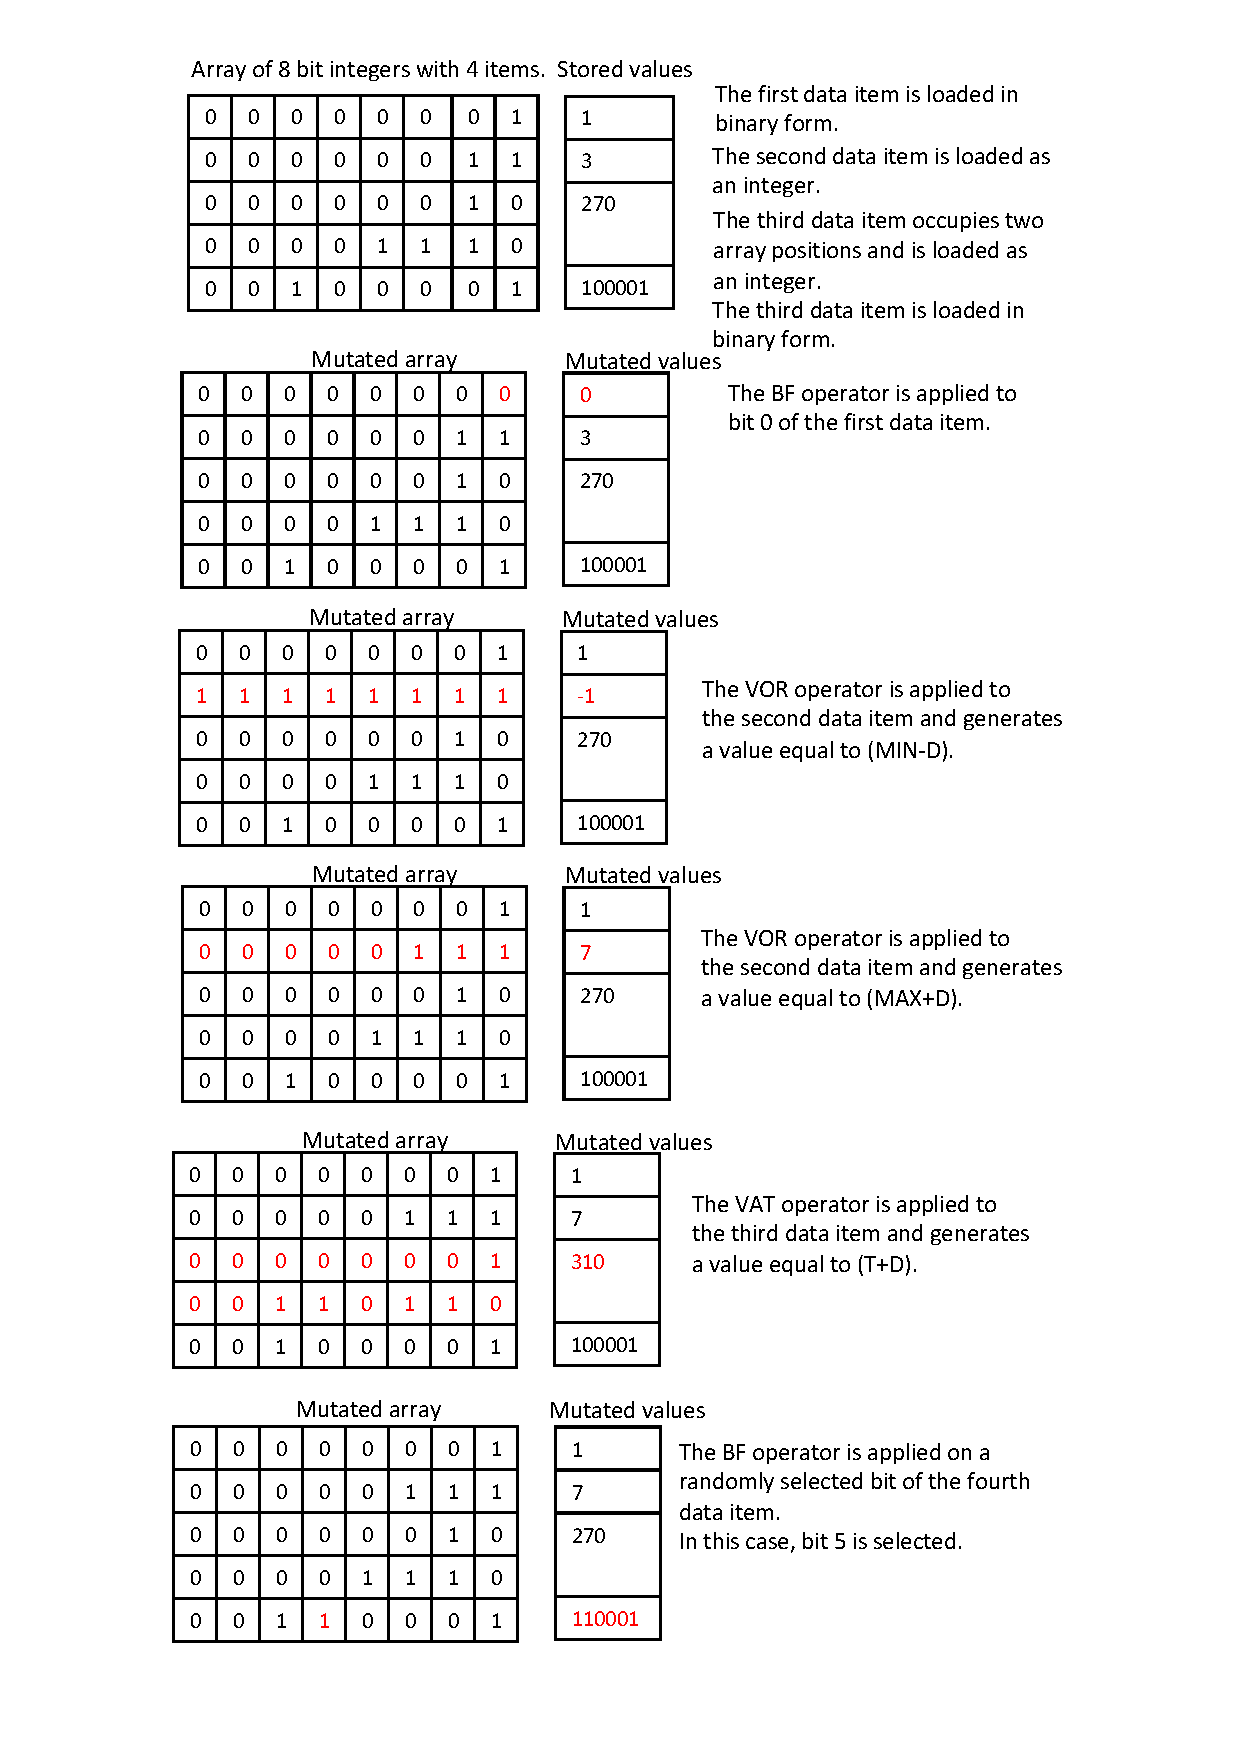
\includegraphics[width=12cm]{images/dataMutationFMExample.pdf}
      \caption{Example of original data and  data mutated according to the fault model in Table~\ref{table:faultModel:example}.}
      \label{fig:dataMutationFMExamples}
\end{figure}





\clearpage


\subsubsection{Automated Generation of Mutation API (Step 2) and Probe Insertion (Step 3)}
\label{sec:generateAPI}

\begin{figure}[tb]
\centering
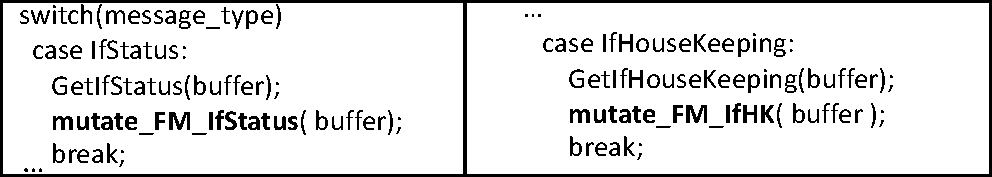
\includegraphics[width=7cm]{damat/images/ProbesExample}
\caption{Example of \APPR mutation probes (in bold).}
\label{fig:appr:ProbesExample}
\end{figure}

\APPR automatically generates a \INDEX{mutation API} to perform mutations at runtime. The API implements a set of functions (called \INDEX{mutate\_FM\_<name>}) that mutate a data buffer according to the given fault model. 
These functions select the data item to mutate and the mutation procedure to apply based on the mutant under test (see Section~\ref{sec:mutantsGeneration}). 

The \APPR mutation API works with C/C++ code; however it may be extended to deal with other programming languages.
Since it is not possible to automatically determine which data buffer to mutate, \APPR requires engineers to modify the source code of the CPS under test by introducing a mutation probe which consists of an invocation of the \APPR function that mutates the data buffer according to a specific fault model.
Note that the effort required by the engineer is minimal; indeed, the exchange of data between components is usually managed in a single location (e.g, the function that serializes the data buffer on the network) and thus it is usually sufficient to introduce one function call for each message type to mutate.
Figure~\ref{fig:appr:ProbesExample} shows how the implementation of \ESAIL has been modified to add the mutation probes. 
The SVF function was modified to handle the message requests sent to the ADCS by inserting one mutation probe for each message type to mutate, e.g., IfStatus and IfHouseKeeping in~Figure~\ref{fig:appr:ProbesExample}. 
Function \emph{mutate\_FM\_IfStatus} is part of the generated mutation API; it loads the fault model \emph{IfStatus} into memory (\UPDATED{our API relies on a tree data structure}) and then invokes the function \emph{mutate}. The function \emph{mutate} performs data-driven mutation according to the provided fault model; the implementation of \emph{mutate} is part of the \APPR toolset.



% At a high-level,
%function \emph{mutate} taking into account the size of the data item; it  checks if the 


The behavior of function \emph{mutate} depends on the value of a unique identifier (i.e., the \emph{MutantID}) associated at compile time to the mutant; the \emph{Mutant ID} univocally identifies the performed mutation operation (each mutant executes one mutation operation, see Section~\ref{sec:mutantsGeneration}).
At a high level, \emph{mutate} performs four activities. First, it checks if the mutation should be performed (i.e., if the data buffer is targeted by the mutation operation identified with the \emph{Mutant ID}). Second, it casts the data item instance targeted by the mutant to a support variable of the type specified in the fault model. Third, it mutates the data stored in the support variable; for each mutation operator, we have implemented a distinct set of instructions for each data representation type. Fourth, before terminating, the function \emph{mutate} writes the mutated data back to the data buffer.





\subsubsection{Automated Generation of Mutants (Step 4)}
\label{sec:mutantsGeneration}



Consistent with code-driven mutation analysis, \APPR generates one mutant for each mutation procedure of the mutation operators configured in the fault model. Each mutant performs exactly one \INDEX{data mutation operation} (i.e., a data mutation procedure configured for a specific data item). For example, the specification in row 6 of Table~\ref{table:faultModel} makes \APPR generate two mutants: each mutant modifies the value of the data item starting at position 12 but one mutant replaces the current value with the value 51 (i.e., $50+1$) while the other replaces the current value with the value $-21$ (i.e., $-20 -1$).

The mutant generation is invisible to the end-user who does not need to modify the source code further; indeed, we rely on a C macro to specify, at compile time, which mutation operation must be performed by every mutant. Mutants are generated by compiling the \UPDATED{SUT} multiple times, once for each mutation operation. At runtime, the mutate function executes only the mutation operation selected for the mutant under test.

\subsubsection{Mutants Execution (Step 5)}
\label{sec:mutantsExecution}

As for \INDEX{code-driven mutation analysis}, the test suite under analysis is executed iteratively with every data-driven mutant. 
At runtime, all the data items targeted by a mutant are mutated whenever the mutation preconditions hold (e.g., the STATE of the BF operator); we leave the mutation of a sampled subset of \UPDATED{data item instances to future work~\cite{zhang2013operator,gopinath2015hard}.}

To speed up the mutation analysis process, the test suite under analysis is first executed with a special mutant that, instead of mutating data items, keeps trace of the fault models loaded by each test case; in other words, it traces what are the data types covered by each test case. The collected information enables the execution, for every mutant, of the subset of test cases that cover the 
message type
%type of data 
targeted by the mutant, thus speeding up mutation analysis.


\subsubsection{Mutation Analysis Results (Step 6)}
\label{sec:mutationAnalysisResults}

Inspired by work on \INDEX{abstract mutation analysis}~\cite{Offutt2006}, we have defined three metrics to evaluate test suites with data-driven mutation analysis: \INDEX{fault model coverage}, \INDEX{mutation operation coverage}, and \INDEX{mutation score}. 
%The first two provide information about the quality of test inputs, whereas the latter provides information about the quality of test oracles \CHANGED{and the test process}. Different from code-driven mutation analysis, data-driven mutation analysis thus enables engineers to distinguish between these two distinct problems affecting test suite effectiveness.
These metrics measure the frequency of the following scenarios: (case 1) the message type targeted by a mutant is never exercised, (case 2) the message type is covered by the test suite but it is not possible to perform some of the mutation operations (e.g., because the test suite does not exercise out-of-range cases), (case 3) the mutation is performed but the test suite does not fail.
\CHANGED{Different from code-driven mutation analysis, these three metrics enable engineers to distinguish between possible test suite shortcomings, including untested message types, uncovered input partitions, poor oracle quality, 
%faulty software, 
and lack of test inputs.}

\INDEX{Fault model coverage (FMC)} is the percentage of fault models covered by the test suite. Since we define a fault model for every 
message type exchanged by two components,
%different data buffer (i.e., type of data exchanged by two components), 
it provides information about the extent to which the message types actually exchanged by the SUT are exercised and verified by the test suites. 
%In other words, low fault model coverage indicates that many test scenarios (e.g., a specific sequence of test inputs being sent to the CPS when the environment is in a specific state) are not exercised by a test suite. 
\CHANGED{Since different component functionalities often require different message types, low fault model coverage may indicate that only a small portion of the integrated functionalities have been tested.}

\INDEX{Mutation operation coverage (MOC)} is the percentage of data items that have been mutated at least once, considering only those that belong to the data buffers covered by the test suite. It provides information about the input partitions covered for each data item; for example, the FVOR operator leads to two mutation operations, which are applied only if the observed value is outside range. Otherwise the two mutation operations will not be covered, thus enabling the engineer to identify such shortcoming in the test suite.
%TODO: add example

The \INDEX{mutation score (MS)} is the percentage of mutants killed by the test suite \UPDATED{(i.e., leading to at least one test case failure)} among the mutants that target a fault model and for which at least one mutation operation was successfully performed. It provides information about the quality of test oracles; indeed, a mutant that performs a mutation operation and is not killed (i.e., is \emph{live}) indicates that the test suite cannot detect the effect of the mutation (e.g., the presence of warnings in logs).
% or an unexpected output from the system). 
\CHANGED{Also, a low mutation score may indicate missing test input sequences. Indeed, live mutants may be due to either software faults (e.g., the SUT does not provide the correct output for the mutated data item instance) or the software not being in the required state (e.g., input partitions for data items are covered when the software is paused); in such cases, with appropriate input sequences, the  test suite would have discovered the fault or brought the SUT into the required state. Both poor oracles and lack of inputs indicate flaws in the test case definition process (e.g., the stateful nature of the software was ignored).}

\clearpage
\subsection{Running Examples}
\label{sec:dataDriven:example}

In this Section, we provide a set of running examples that show the results achieved by \APPR in the presence of test suites affected by different problems. More precisely we aim to demonstrate, for representative cases, the absence of false alarms due to equivalent mutants and the usefulness of the mutation analysis metrics computed. 
\REVTOOL{P-3}{Each running example is an artificial but realistic definition of test suites to illustrate the methodology.}
We consider the following representative scenarios:
\begin{enumerate}
\item The test suite exercises only one message exchange between the ADCS and the SUT; each test case covers a distinct input partition.
\item The test suite exercises only one message exchange between the ADCS and the SUT; multiple test cases cover a same input partition.
\item The test suite exercises multiple message exchanges between the ADCS and the SUT; each test case covers a distinct combination of input partitions.
\end{enumerate}


\subsubsection{Example set 1: One message exchange, distinct input partitions}
\label{sec:dataDriven:example:1}

\begin{figure}[tb]
\centering
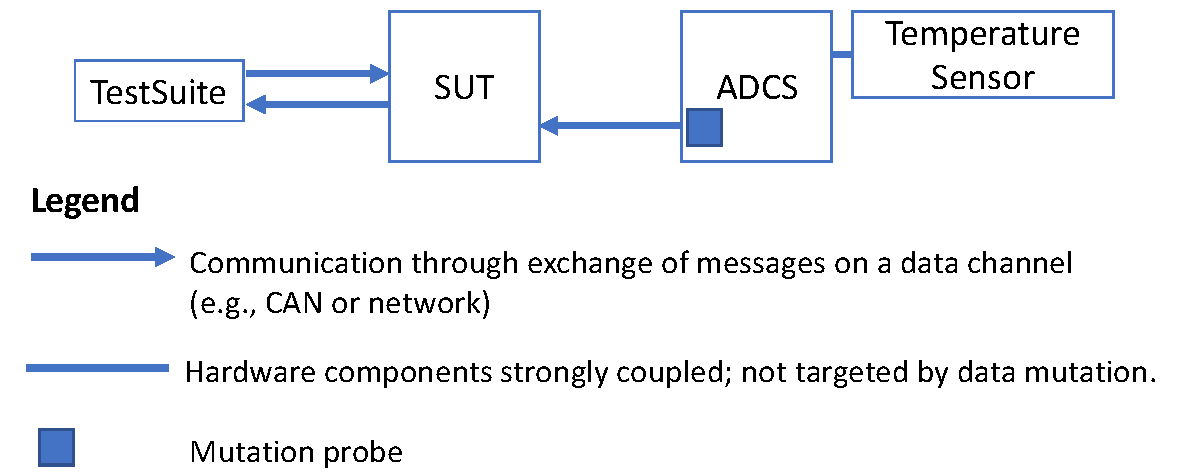
\includegraphics[width=8cm]{damat/RunningExampleArch}
\caption{Architecture of the running example system.}
\label{fig:damat:RunningExampleArch}
\end{figure}

Our first set of running examples concerns the presence of a single message exchange and test cases covering distinct input partitions.

Our examples concern an SUT that exchanges with the ADCS component one type of message. More precisely, the ADCS sends a message (hereafter, \emph{TempMessage}) with the temperature collected by its sensor. The architecture of such system is shown in Figure~\ref{fig:damat:RunningExampleArch}. For simplicity, we assume that the ADCS periodically sends a TempMessage to the SUT. The ADCS is connected to the TemperatureSensor. The communication between the ADCS and the TemperatureSensor is not affected by data-driven mutation. We may assume the ADCS and the TemepratureSensor are simulated during the execution of the test suite. The SUT and the ADCS communicate through a channel 
(e.g., a CAN bus). The data mutation probe is inserted in the ADCS simulator; in practice we mutate the data generated by the ADCS. The test suite exercises the software under test by communicating through a data channel; the type of communication channel used by the test suite is not relevant for the purpose of the running example.

For our running example, the SUT has two state variables that are observable by the test suite, \emph{temperature} and \emph{temperature\_alarm}. The state variable \emph{temperature} reports the temperature returned by the sensor in the last message. 
The state variable \emph{temperature\_alarm} is set to 1 if the temperature returned by the sensor is above 100.

The test suite is comprised of two test cases. \emph{Test 1} exercises the SUT with a temperature in the nominal case (i.e., temperature below 100), \emph{Test 2} concerns the non nominal case (i.e., temperature above 100). The two test cases of the test suite exercise the same sequence of interactions, which are depicted in the UML Sequence diagram of Figure~\ref{fig:damat:RunningExample1Sequence}. The sequence diagram shows that the test case first starts the ADCS simulator and the SUT; then, it waits for the ADCS to send the TempMessage before requesting the values of the variables \emph{temperature} and \emph{temperature\_alarm}. Figure~\ref{fig:damat:RunningExample1Sequence} also shows that, in this case, the mutation is performed within the ADCS simulator.

\begin{figure}[tb]
\centering
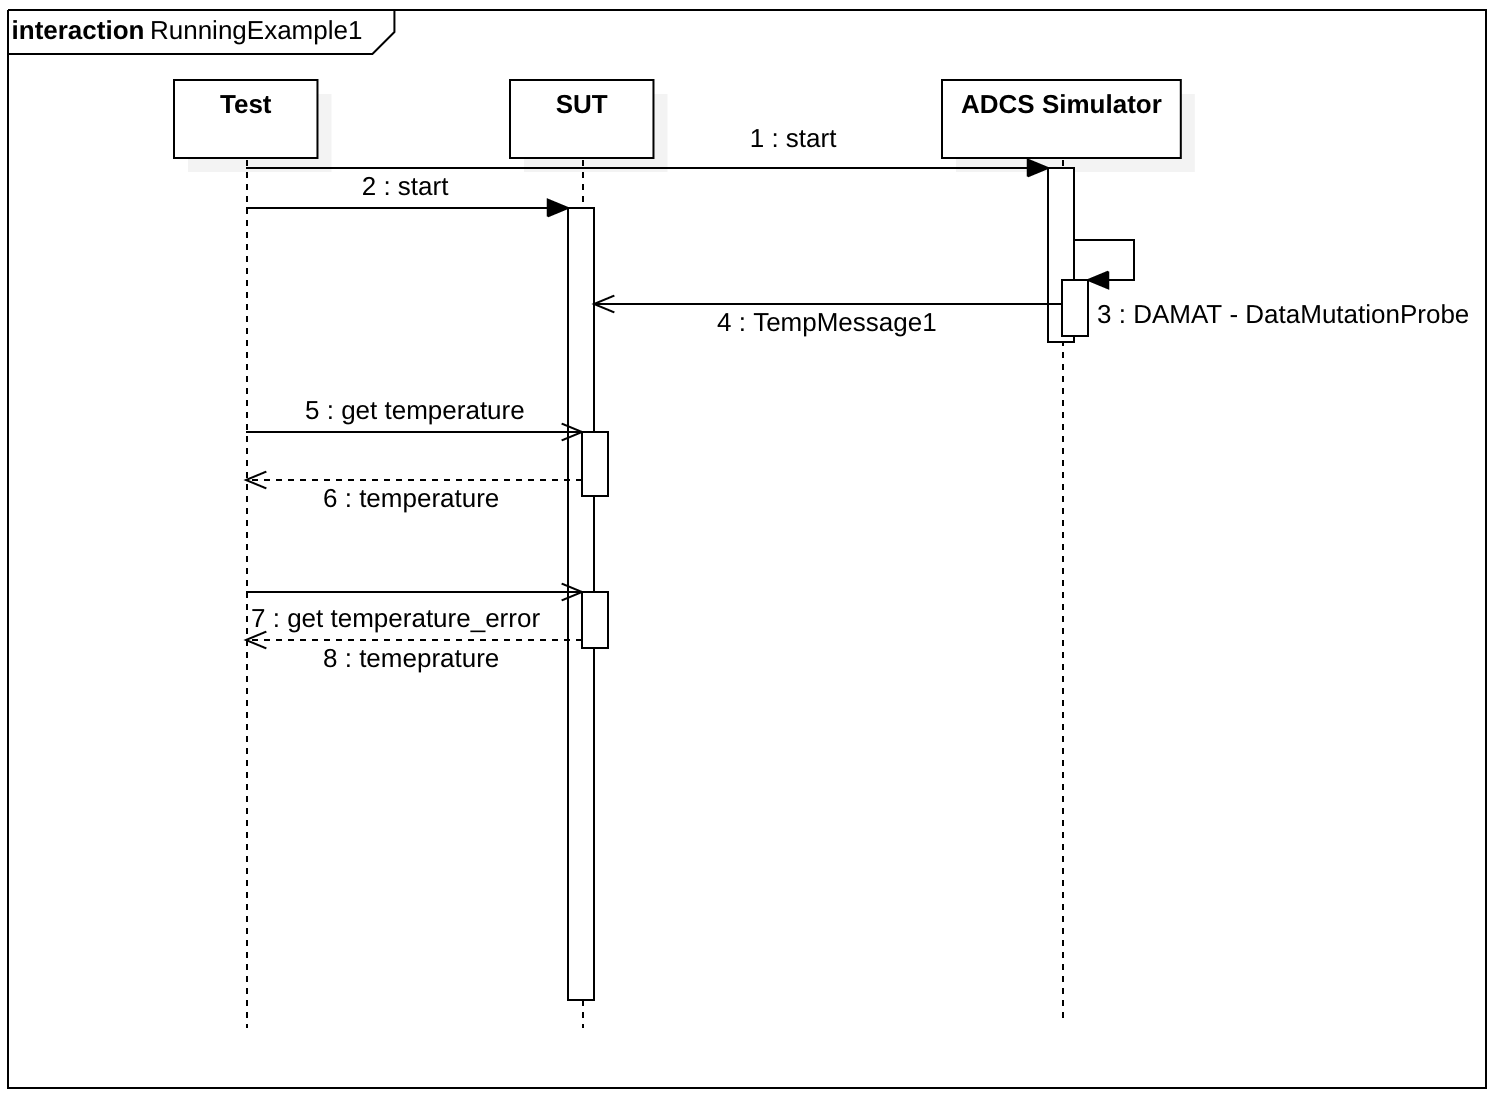
\includegraphics[width=8cm]{damat/images/runningExamplesSequence1.png}
\caption{Interactions exercised by the test cases belonging to the running example set 1.}
\label{fig:damat:RunningExample1Sequence}
\end{figure}


Figures~\ref{fig:damat:RunningExample1A} to~\ref{fig:damat:RunningExample1C} show our running examples. On the top, we report the fault model. In this case the fault model applies the operators VAT (value above threshold) and FVAT (fix value above threshold). The VAT operator is configured with a threshold of 100 and a delta of 10 (i.e., it replaces values below the threshold with the value 110). The FVAT operator is configured in the same manner (i.e., it replaces values above threshold with the value 90). The operator VAT leads to \emph{MUTANT 1}, the operator FVAT leads to \emph{MUTANT 2}; \REVTOOL{P-5}{to summarize, in this example we have two mutants, each implements one distinct mutation operator.}

In Figure~\ref{fig:damat:RunningExample1A}, under \emph{Exchanged data}, we report the sequence of data messages exchanged by the test cases of the test suite (one column for each test case).
In the following rows, we report the oracles. For each oracle we indicate how it verifies if a state variable has been assigned with a correct value; we indicate $"=="$ if it verifies the exact value taken by the state variable (e.g., \emph{temperature == 50)}, "$>=$" if it verifies that the value is above a threshold (e.g., \emph{temperature $>=$ 50}). Please note that, according to standard practice, test cases for non nominal cases verify that state variables contain the expected alarm and anomalous values (i.e., the test case passes only if the SUT report the anomaly). 

For each mutant, we report the value of the data exchanged during the execution and the data of the state variables read by the oracle. In red we indicate data that has been mutated according to the fault model. 
If an oracle does not read the value of a variable we leave the cell empty.
Failing oracles are highlighted in yellow.
\REVTOOL{P-5}{Note that for each mutant we provide multiple columns (named \emph{Test 1} and \emph{Test 2}), each provides the data exchanged during the execution of the test case.}
Finally, for each mutant, for each oracle, we report the test cases that detect the anomalous value (if any); also, we report if the mutant had been killed.


Please note that, following the \APPR procedures, MUTANT 1 does not mutate the data exchanged by Test 2 because it is already above the threshold. MUTANT 2 does not mutate the data exchanged by Test 1 because it is already below the threshold.

TestSuite1 is an optimal test suite that verifies the expected value of all the state variables. For MUTANT 1, Test 1 fails because the assertion about temperature fails (expected 50 observed 110).
For MUTANT 2, Test 2 fails because the assertion about temperature fails (expected 120 observed 90).
\REVTOOL{P-6}{We have a fault model coverage (\emph{FMC}) of 100\% because we have only one fault model and it is covered (i.e., the test suite exchanged the data message under analysis). We have a mutation operator coverage (\emph{MOC}) of 100\% because all the mutation operations associated with the configured mutation operators are applied (in other words, all the mutants perform at least one mutation of a data item instance). We have a mutation score (\emph{MS}) of 100\% because, for each mutant, at least one test case fails.}

TestSuite2 verifies the expected value of the temperature for the nominal case and the presence of a temperature error for the non nominal case. For MUTANT 1, Test 1 fails because the assertion on temperature fails (expected 50 observed 110).
For MUTANT 2, Test 2 fails because the assertion on temperature errors fail (expected 1 observed 0).
\REVTOOL{P-6}{Concerning FMC, MOC, and MS, the same considerations made for TestSuite1 hold.}

TestSuite3 verifies only temperature values while TestSuite4 verifies only temperature alarms. They all kill the mutants for the same reasons reported in the cases above. \REVTOOL{P-6}{Concerning FMC, MOC, and MS, the same considerations made for TestSuite1 hold.}


TestSuite5 is a copy of TestSuite2 having an imprecise oracle (i.e., it verifies that temperature is above 50 instead of equal to 50). Consequently the test suite does not fail for MUTANT 1 and the mutation score is not 100\%; consequently, \APPR enables an engineer to detect the limitation of the test suite.

\REVTOOL{P-6}{TestSuite6} is a copy of TestSuite2 without an oracle for Test2 (i.e., it does not verify the presence of temperature alarms). Consequently, the test suite does not fail for MUTANT 2 and the mutation score is not 100\%; consequently, \APPR enables an engineer to detect the limitation of the test suite.

TestSuite7 is a copy of TestSuite2 with multiple test cases covering the same input partitions; indeed, Test3 covers the same input partition of Test1 (i.e., it exercises the value 0, which is a nominal value like 50), Test4 covers the same input partition of Test2 (i.e., it exercises the value 101, which is a non nominal value like 120). All the mutants are killed by the test suite and we do not observe equivalent mutants.

TestSuite8 is a copy of TestSuite7 with the same limitations of TestSuite6 (i.e., Test2 does not contain an oracle).
In this case, the mutation score is 100\% because Test 4 contains an appropriate oracle and covers the same input partition not appropriately verified by Test 2. We do not observe equivalent mutants.

TestSuite9 is a copy of TestSuite7 without oracles for both Test2 and Test4; similarly to the case of TestSuite6, since the non-nominal partition is not appropriately verified, the mutation score is not 100\%; consequently, \APPR enables an engineer to detect the limitation of the test suite.

TestSuite10 covers the case of a test suite that does not exercise an input partition; precisely, it does not exercise non nominal values. 
In this case, \APPR can detect that MUTANT 2 is never applied (to exemplify it, we do not report any red value for MUTANT 2 in Figure~\ref{fig:damat:RunningExample1C}); consequently, the MOC is not 100\% and the engineer can determine what is the limitation of the test suite. Indeed, since the mutant not covered is FVAT, the engineer can know that the test suite does not exercise the value above threshold for the temperature (FVAT applies the mutation only if a value above threshold is observed).

\begin{figure}[tb]
\centering
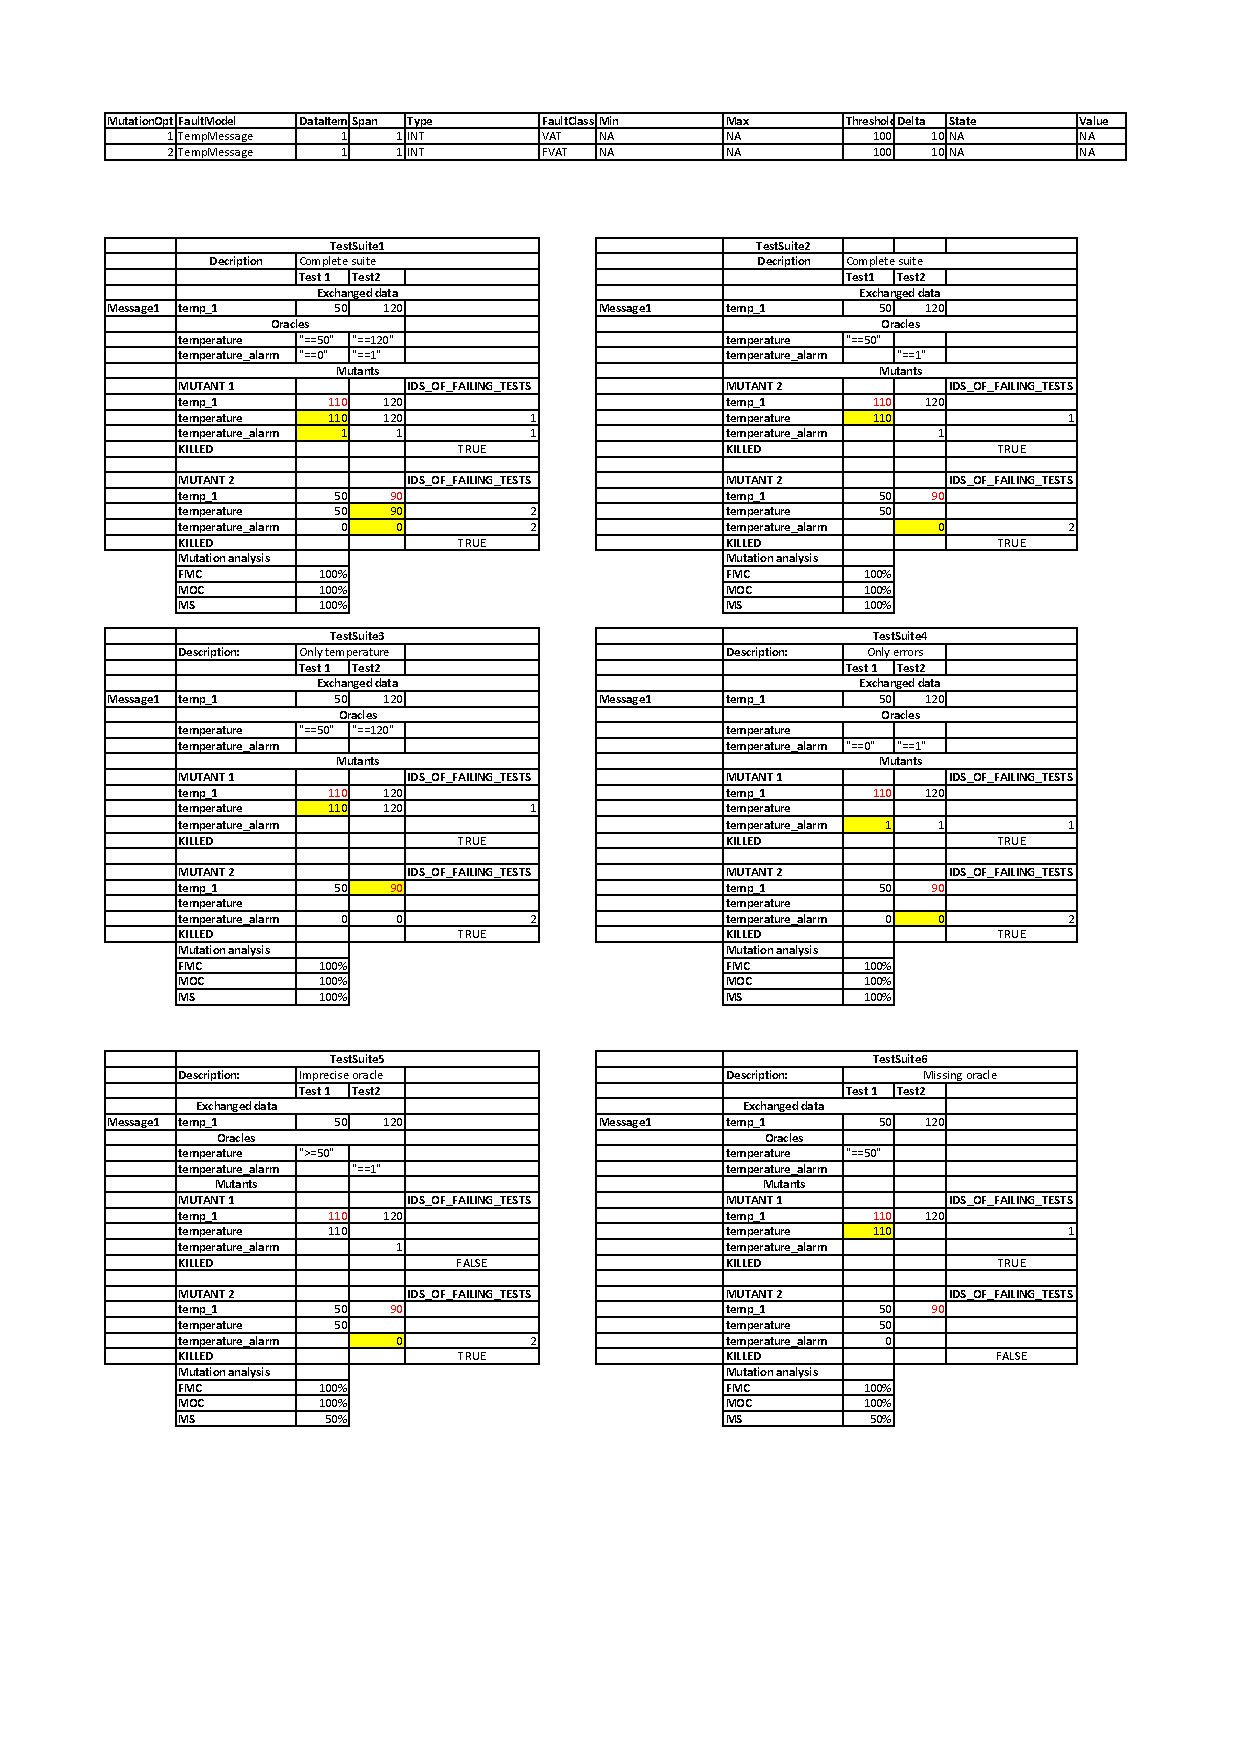
\includegraphics[width=18cm]{damat/DataDrivenExample1A}
\caption{Running example set 1 - Part A.}
\label{fig:damat:RunningExample1A}
\end{figure}

\begin{figure}[tb]
\centering
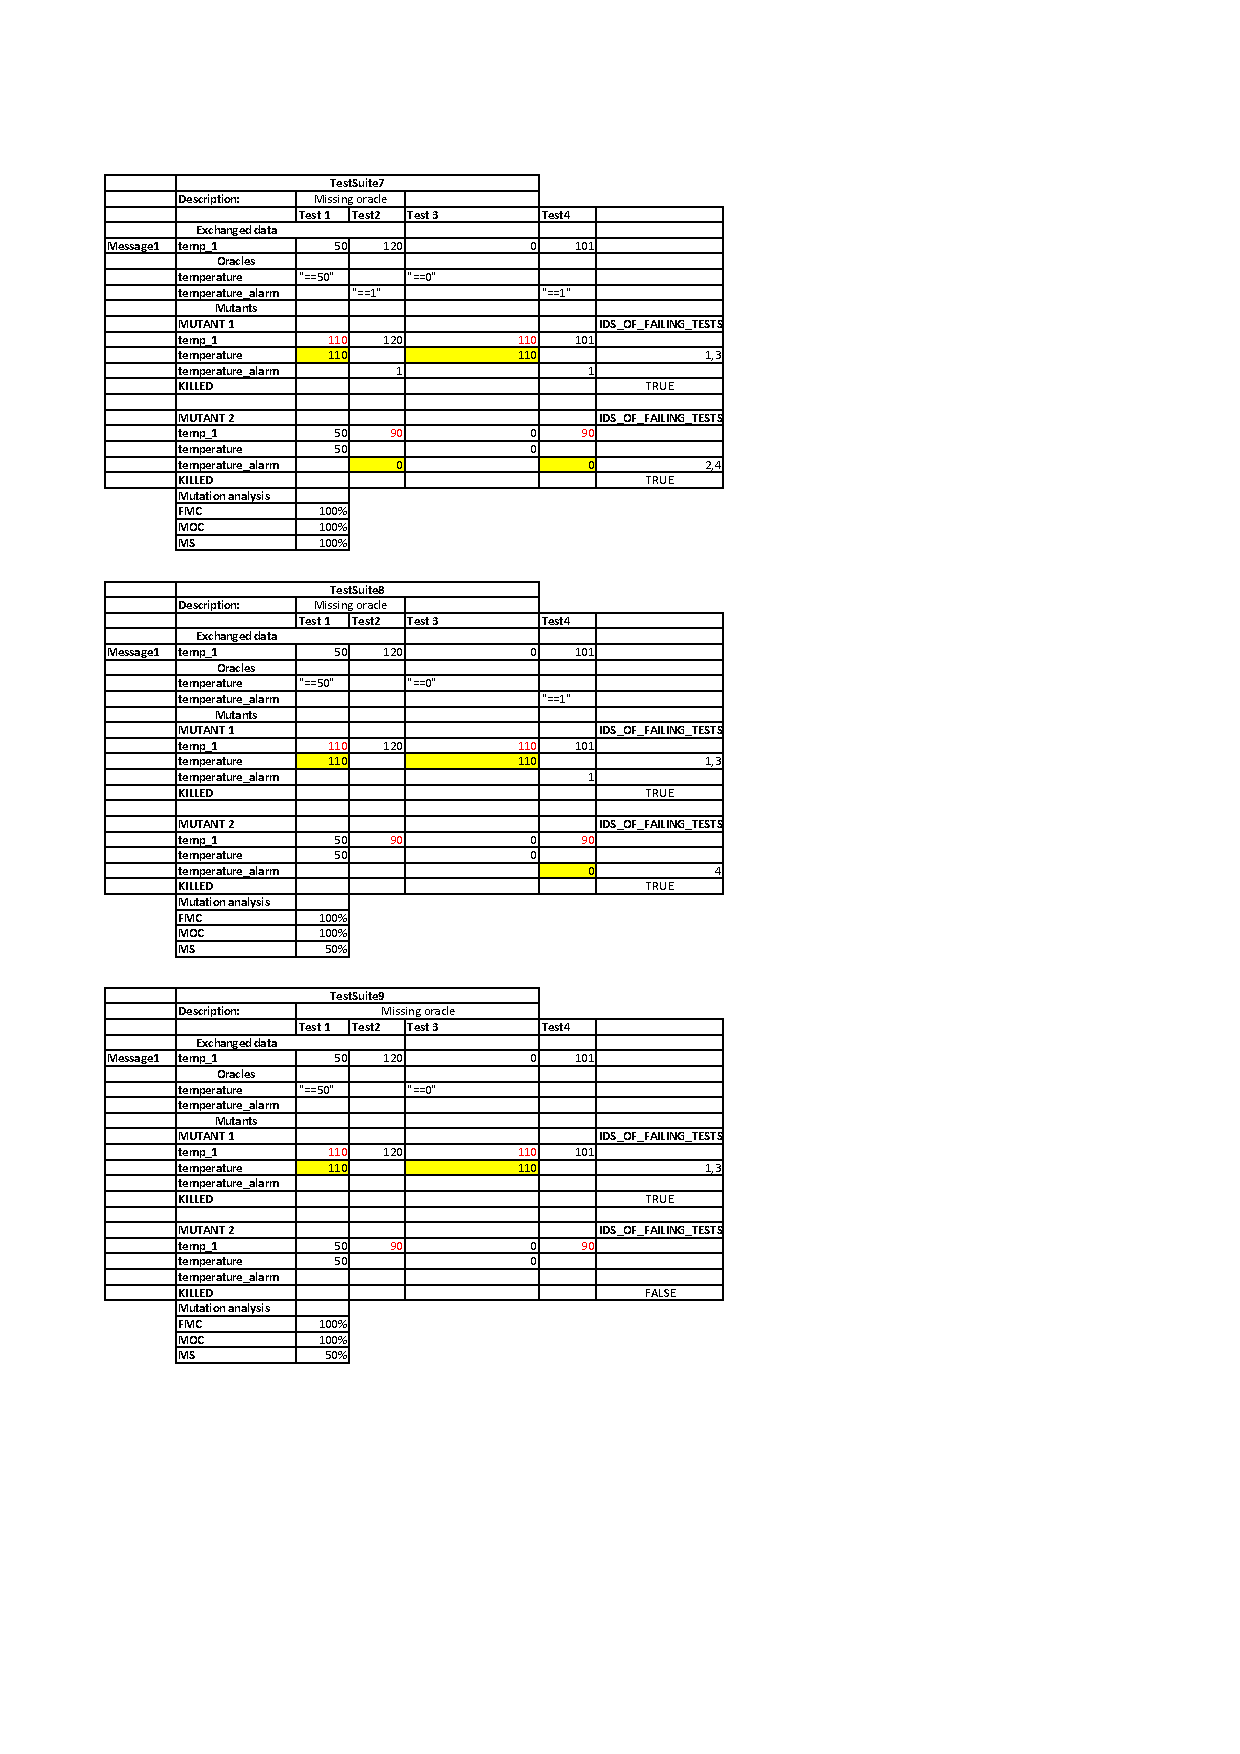
\includegraphics[width=18cm]{damat/DataDrivenExample1B}
\caption{Running example set 1 - Part B.}
\label{fig:damat:RunningExample1B}
\end{figure}

\begin{figure}[tb]
\centering
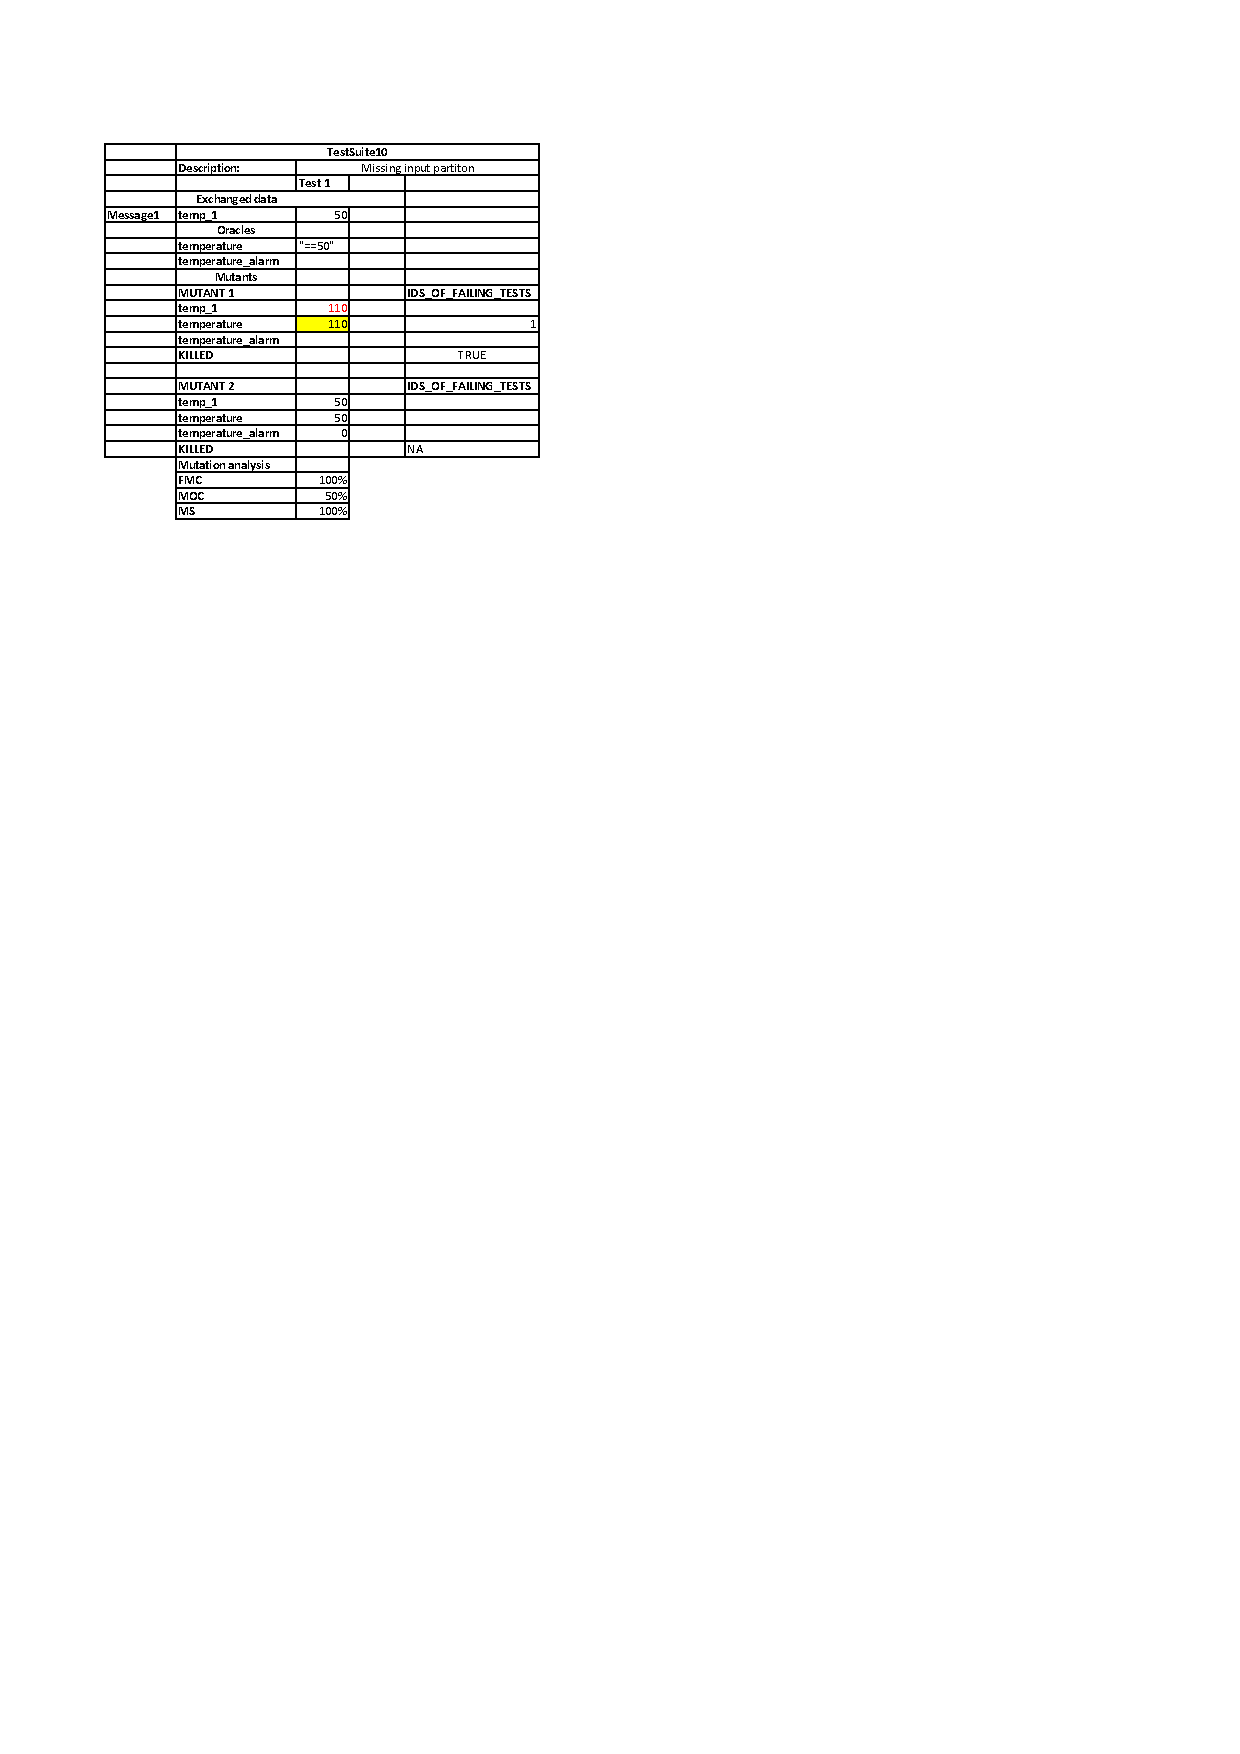
\includegraphics[width=18cm]{damat/DataDrivenExample1C}
\caption{Running example set 1 - Part C.}
\label{fig:damat:RunningExample1C}
\end{figure}

%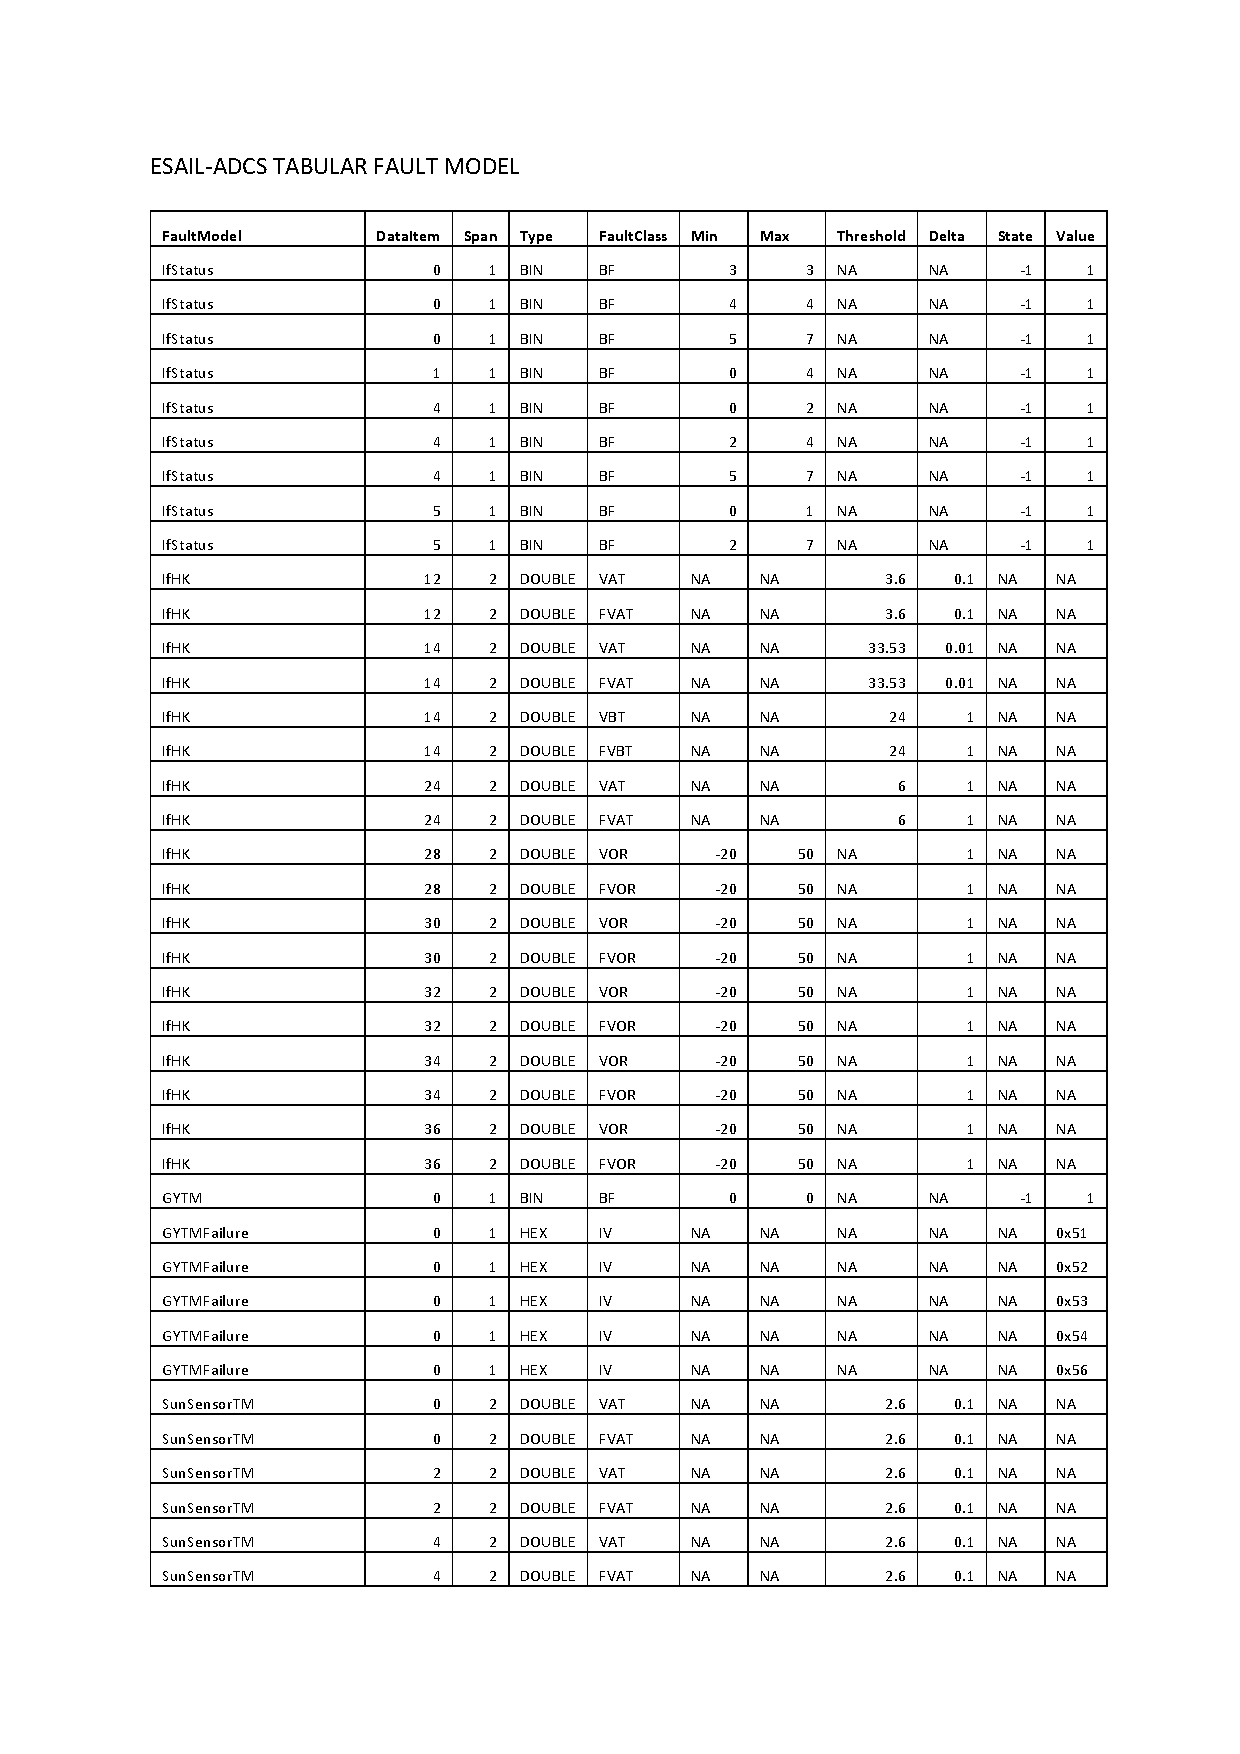
\includepdf[pages=-,scale=0.9,offset=0mm -75]{faultModels/FaultModels.pdf}

\clearpage

\subsubsection{Example set 2: One message exchange, distinct input partitions, faulty software}
\label{sec:dataDriven:example:2}

This running example (see Figure~\ref{fig:damat:RunningExample2}) covers the same case of Section~\ref{sec:dataDriven:example:1}, with the difference that we assume the software to be faulty. More precisely, we assume that the value of \emph{temperature alarm} is always set to 0. We ignore the test suites number 1, 2, 4, 5, 6, 7, 8 because they would detect the presence of the fault before mutation analysis (i.e., the oracles "==1" would fail). For completeness, in Figure~\ref{fig:damat:RunningExample2}, we report the values of state variables also when they are not verified by oracles. We highlight failing oracles in yellow.

For TestSuite6 and TestSuite9, which do not detect the fault because they lack an oracle for the faulty variable, \APPR would indicate that MUTANT 2 is not killed thus enabling the engineer to introduce an appropriate oracle (i.e., "temperature\_alarm == 1") and thus discover the fault. 

For TestSuite3, \APPR would not help the engineer in detecting the fault because the test suite kills the mutant. What we observe in this case is a sort of masking effect due to the fact that two outputs are affected by the same data; indeed, \APPR ensures that the effect of data mutation is propagated to at least one software output but it cannot verify that the effects of data mutation are propagated to all the software outputs that depend on the mutated data. 
%In this specific case, we would like to highlight that a correct test case would have verified first the presence of temperature_alarms. 
%For the detection of algorithmic faults, code-driven mutation analysis might be more appropriate.

\begin{figure}[tb]
\centering
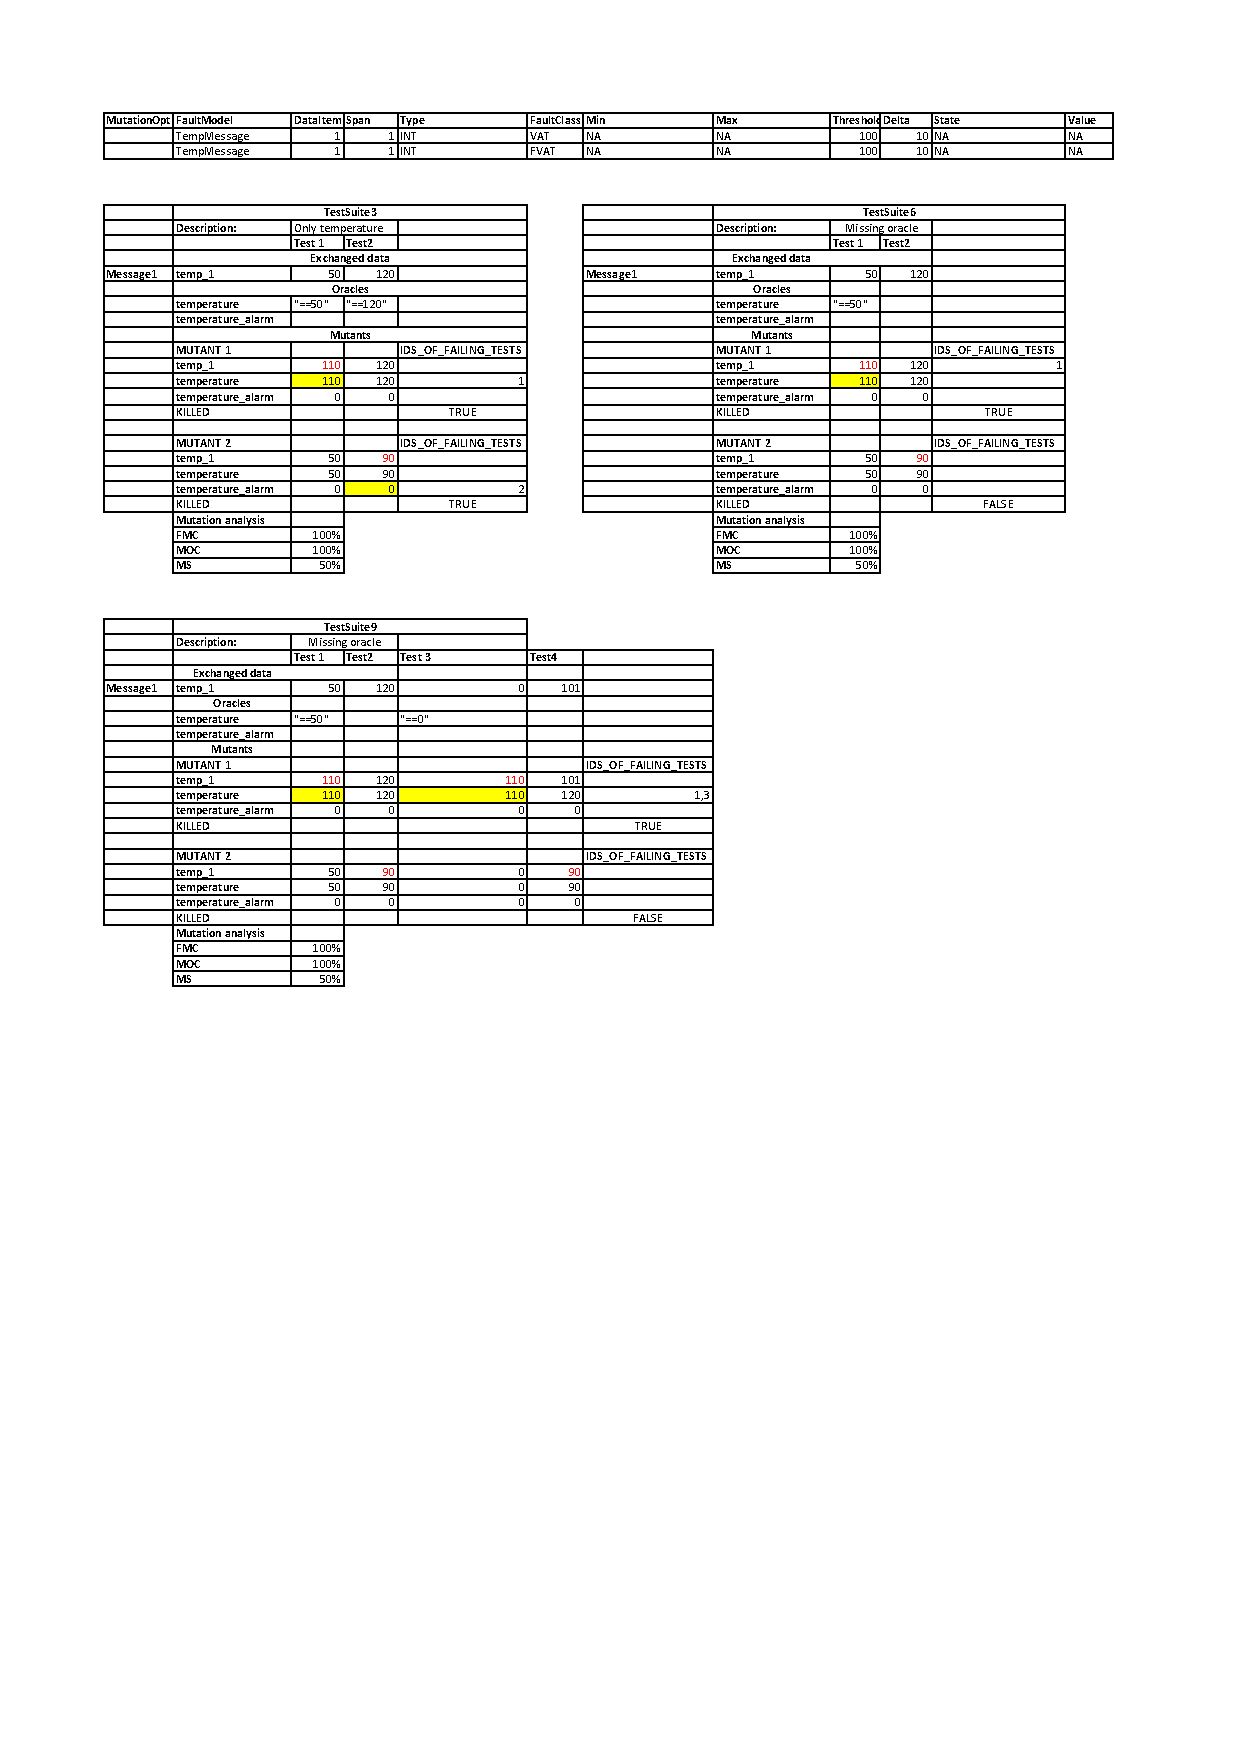
\includegraphics[width=14cm]{damat/DataDrivenExample2}
\caption{Running example set 2.}
\label{fig:damat:RunningExample2}
\end{figure}

\clearpage 
\subsubsection{Example set 3: Multiple message exchanges, distinct input partitions}
\label{sec:dataDriven:example:3}

For the third running example set, we consider a system that has the same architecture of  Figure~\ref{fig:damat:RunningExampleArch} but exchanges also messages of type \emph{BoardStatus}. We assume that \emph{BoardStatus} messages indicate the voltage of the board and the sensors. The SUT has an additional output state variable called \emph{voltage\_error}. A voltage error occurs when the voltage is out of the range (10;14). In the presence of a voltage error, the software shall not update the value of the \emph{temperature} state variable.

Below we discuss two possible test suites, TestSuite1 and TestSuite2, which are affected by different type of limitations.
More precisely, we rely on TestSuite1 to (1) show how \APPR spot a test suite shortcoming difficult to determine manually and (2) demonstrate that \APPR may unlikely lead to equivalent mutants (i.e., by showing that if a mutant is not killed it's because relevant assertions are missing). We rely on TestSuite2 to exemplify the case of lack of coverage of a fault model.

\paragraph{TestSuite1}

Figure~\ref{fig:damat:RunningExample3Sequence} shows the interactions exercised by the test cases in the test suite named TestSuite1 for the running example set 3. Each test case, after starting the ADCS simulator and SUT, waits till the ADCS has sent the following sequence of messages: one BoardStatus message, one TempMessage, one BoardStatus message, and one TempMessage. Then it requests and verifies the values of the state variables \emph{temperature}, \emph{temperature\_alarm}, and \emph{voltage\_error}.

\begin{figure}[tb]
\centering
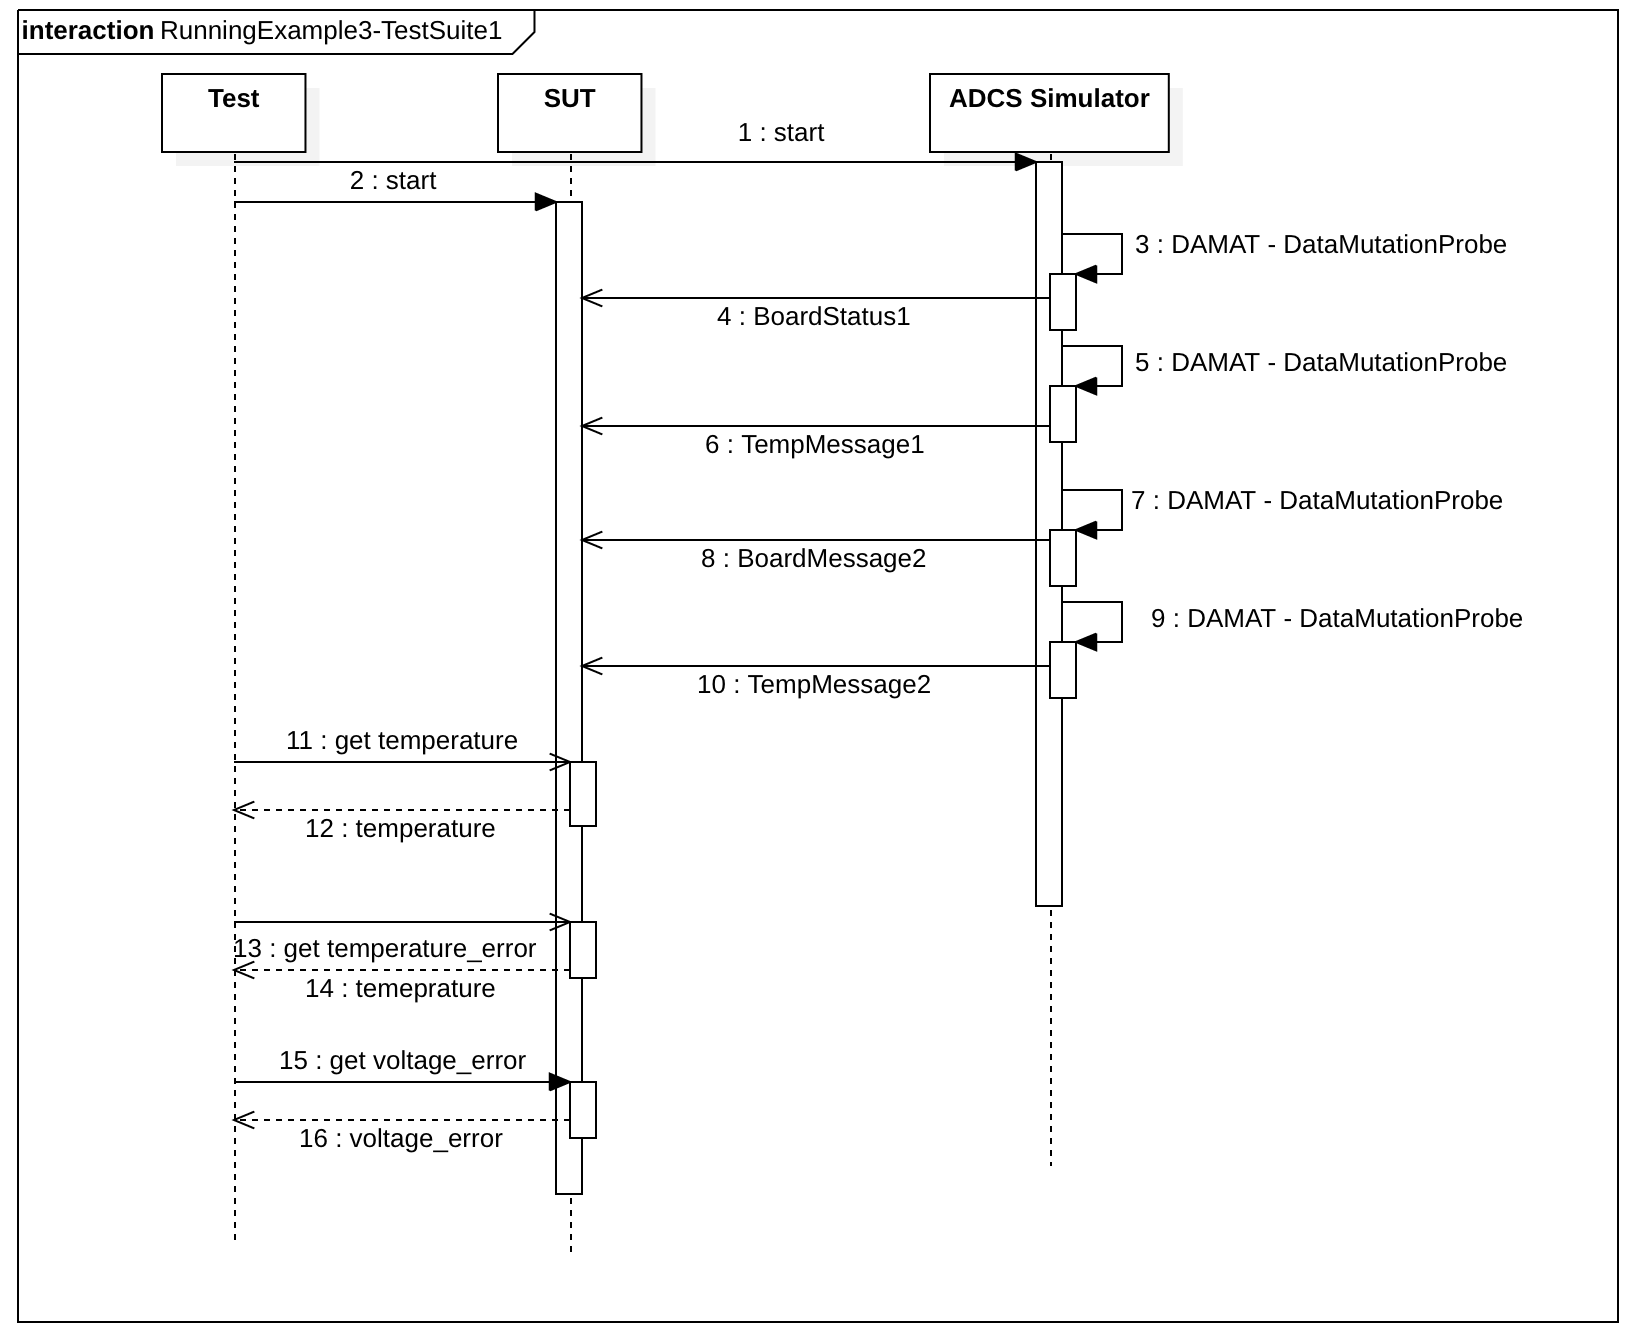
\includegraphics[width=8cm]{damat/images/RunningExampleSequence3.png}
\caption{Interactions exercised by the test cases of TestSuite1 in the running example set 3.}
\label{fig:damat:RunningExample3Sequence}
\end{figure}

Figures~\ref{fig:damat:RunningExample3A} and~\ref{fig:damat:RunningExample3B} show the data exchanged in our running example. With respect to the example set 1, the fault model includes also one VOR and FVOR operator to mutate the BoardStatus message. In Figures~\ref{fig:damat:RunningExample3A} and~\ref{fig:damat:RunningExample3B}, in the row named \emph{PASS}, we explicitly indicate the result of each test case (i.e., PASS or FAIL).

TestSuite1 covers all the possible combinations of values for the sequence of messages reporting about messages voltage error absent (true or false), temperature alarm absent (true or false), voltage error absent (true or false), temperature alarm absent (true or false); indeed, in total, we have 16 test cases.

TestSuite1 kills MUTANT 1. MUTANT 1 applies VAT, that is, it sets the temperature value above the threshold when it is below the threshold. To not kill MUTANT 1, the test suite should not include any failing oracle. Since the failing oracles include the complete set of oracles that either verify the temperature being in the nominal range or verify the absence of a temperature alarm, we conclude that whenever MUTANT 1 is not killed, we cannot be in the presence of an equivalent mutant but in the presence of a test suite limitation.

TestSuite1 kills MUTANT 2. MUTANT 2 applies FVAT, that is, it sets the temperature value below the threshold when it is above the threshold. To not kill MUTANT 2, the test suite shall not include any of the failing oracles. Since the failing oracles include the complete set of oracles that either verify the temperature being out of the nominal range or verify the presence of a temperature alarm, we conclude that whenever MUTANT 2 is not killed, we cannot be in the presence of an equivalent mutant but in the presence of a test suite limitation.

TestSuite1 kills MUTANT 3. MUTANT 3 applies the first mutation procedure of VOR, that is, it sets the value above range if it is within range. To not kill MUTANT 2, the test suite shall not include any of the failing oracles. Since the failing oracles include the complete set of oracles that either verify the temperature being in the nominal range or verify the absence of a temperature alarm, we conclude that whenever MUTANT 3 is not killed, we cannot be in the presence of an equivalent mutant but in the presence of a test suite limitation.

TestSuite1 kills MUTANT 4. MUTANT 4 applies the second mutation procedure of VOR, that is, it sets the value below range if it is in range. MUTANT 4 leads to the same system outputs as MUTANT 3 thus we can make the same conclusion (no equivalent mutant possible).

TestSuite1 kills MUTANT 5. MUTANT 5 applies the first mutation procedure of FVOR, that is, it sets the value within range if it is above range. 
To not kill MUTANT 5, the test suite shall not include any of the failing oracles. All the failing oracles belong to test cases that verify a scenario in which a voltage error is present just before the last temperature message is collected; consequently, the lack of such oracles would indicate a major limitation of the test suites (i.e., it would not test if the software identifies the error condition simulated by the scenario under test). Similarly, MUTANT 5 is killed if all such test cases would be missing; even in this case we would be in the presence of a major test suite limitation (i.e., the test suite does not simulate an important error condition). We thus conclude that MUTANT 5 cannot lead to equivalent mutants. 

TestSuite1 does not kill MUTANT 6. MUTANT 6 applies the second mutation procedure of FVOR, that is, it sets the value in range if it is below range. Since no values below range are observed during the execution of the test cases, \APPR never applies this mutation operation. For this reason the mutation operation for the test suite is 83\% (i.e., five out of six mutation operation are covered). Although TestSuite1 seems complete because it tests all the pairwise combinations of the conditions \emph{voltage error absent} and \emph{temperature alarm absent}, \APPR enables us to determine that when defining the test suite we did not consider the fact that the input partitions for voltage error are three (i.e., voltage within range, voltage above range, and voltage below range) not two (i.e., voltage error absent, voltage error present).




\begin{figure}[tb]
\centering
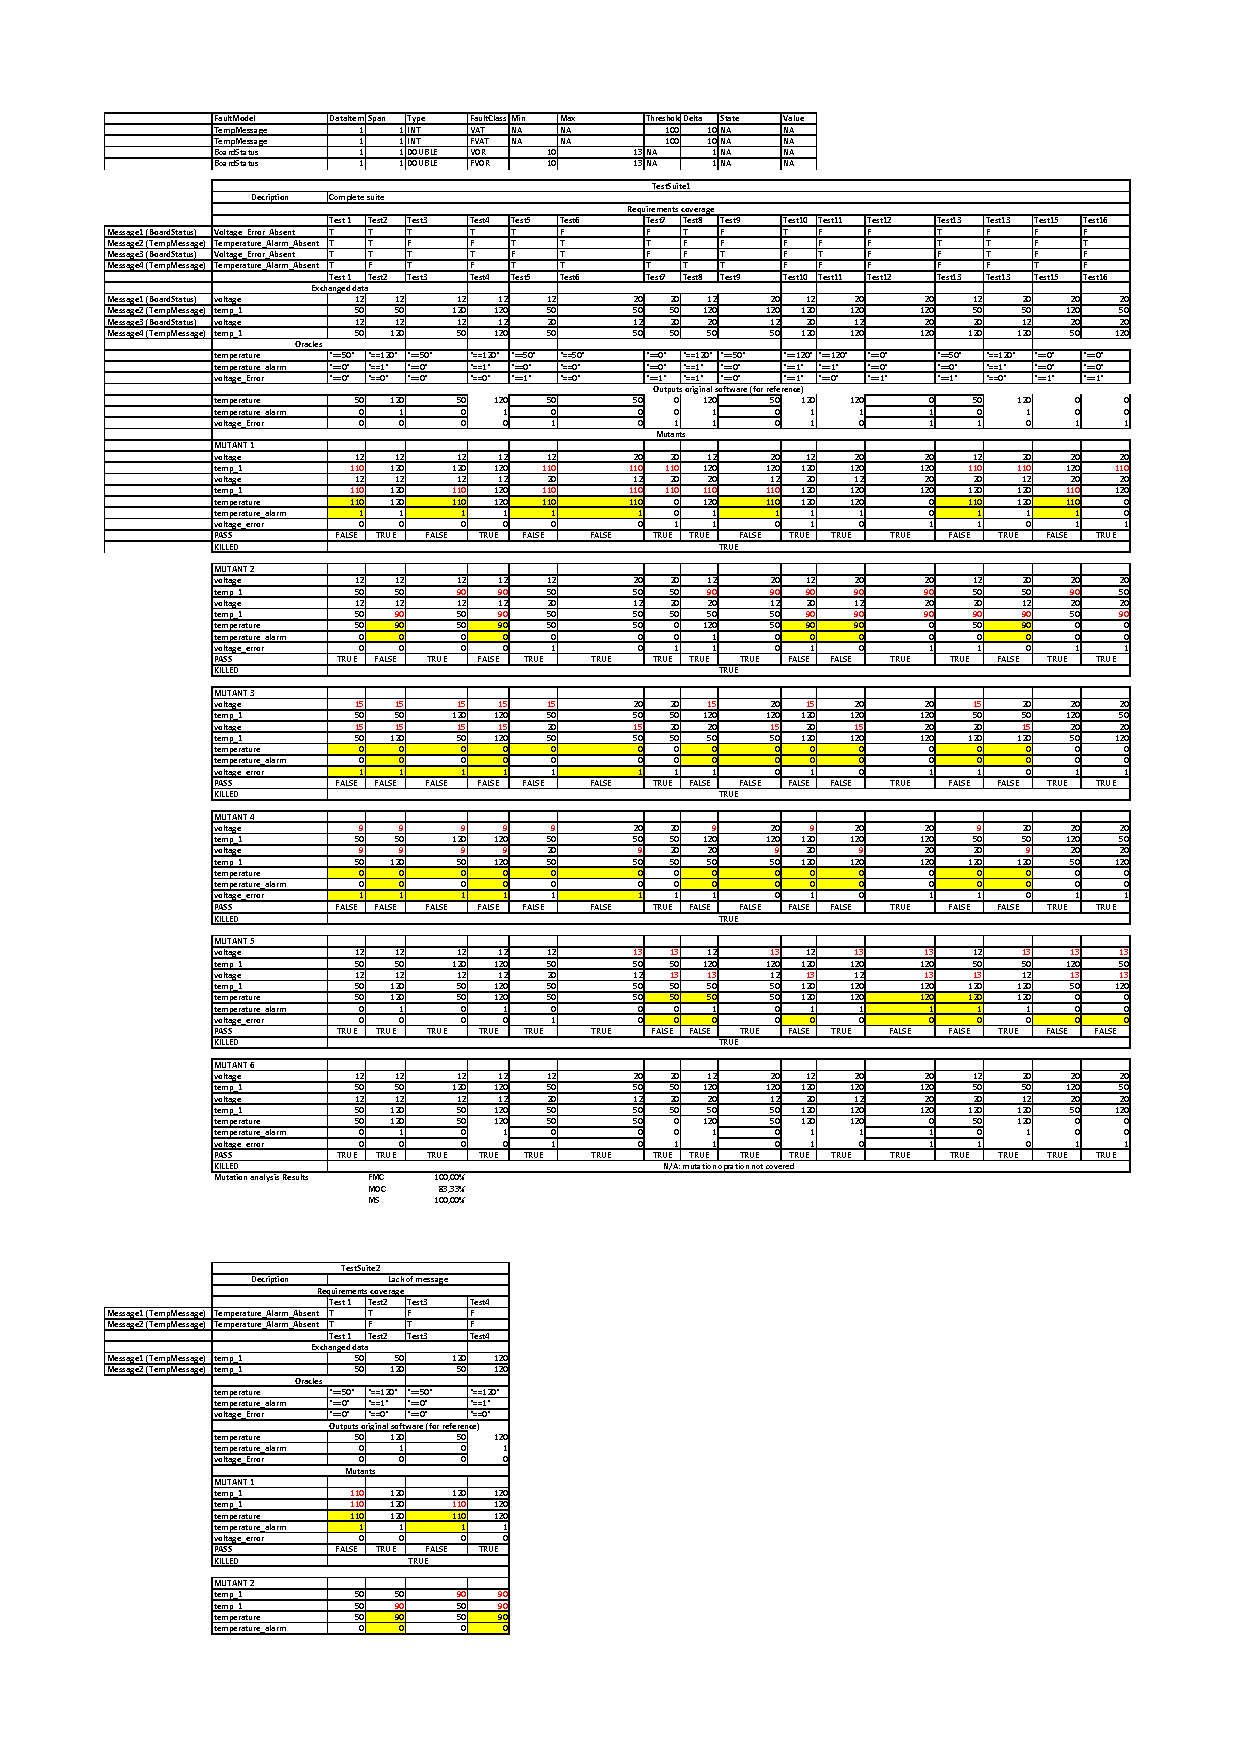
\includegraphics[width=18cm]{damat/DataDrivenExample3A}
\caption{Running example set 3 - Part A.}
\label{fig:damat:RunningExample3A}
\end{figure}

\begin{figure}[tb]
\centering
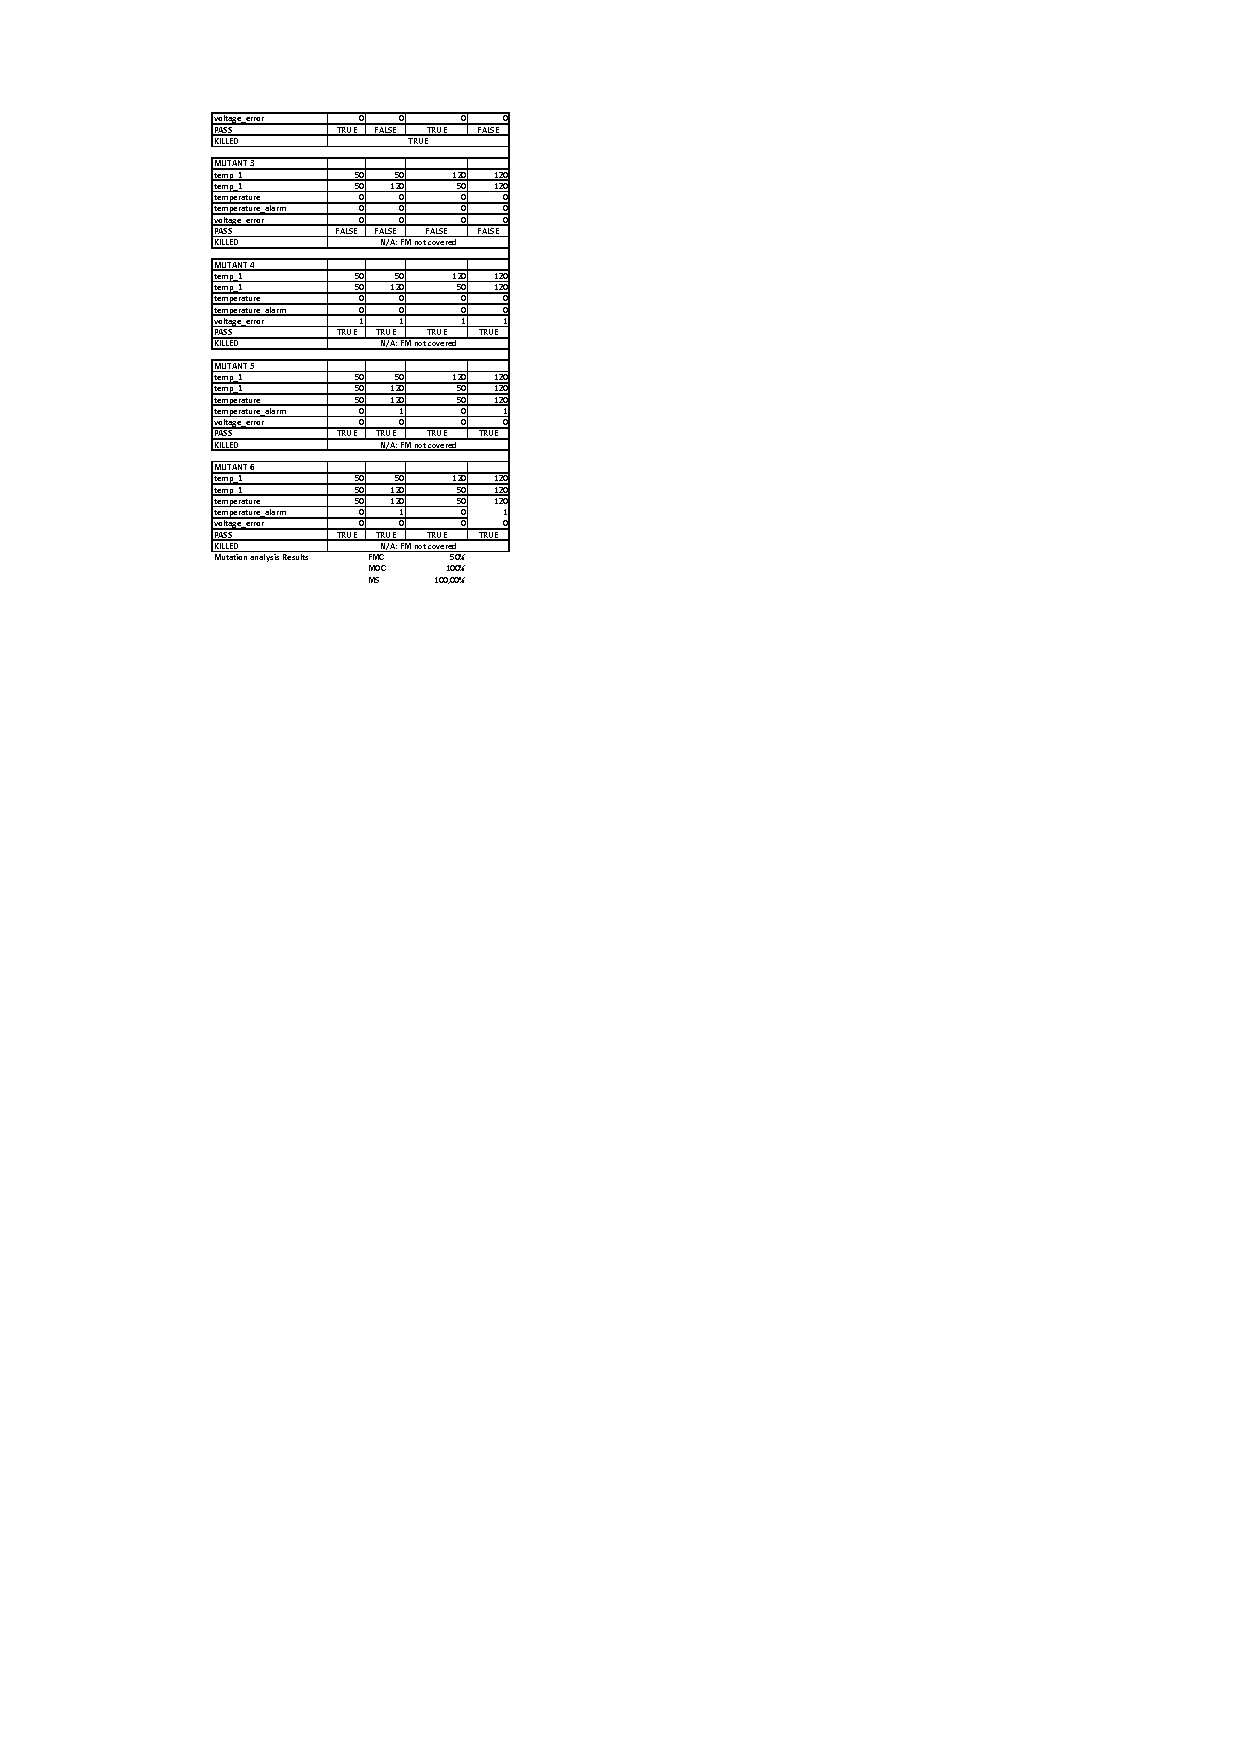
\includegraphics[width=18cm]{damat/DataDrivenExample3B}
\caption{Running example set 3 - Part B.}
\label{fig:damat:RunningExample3B}
\end{figure}


\paragraph{TestSuite2}



\begin{figure}[tb]
\centering
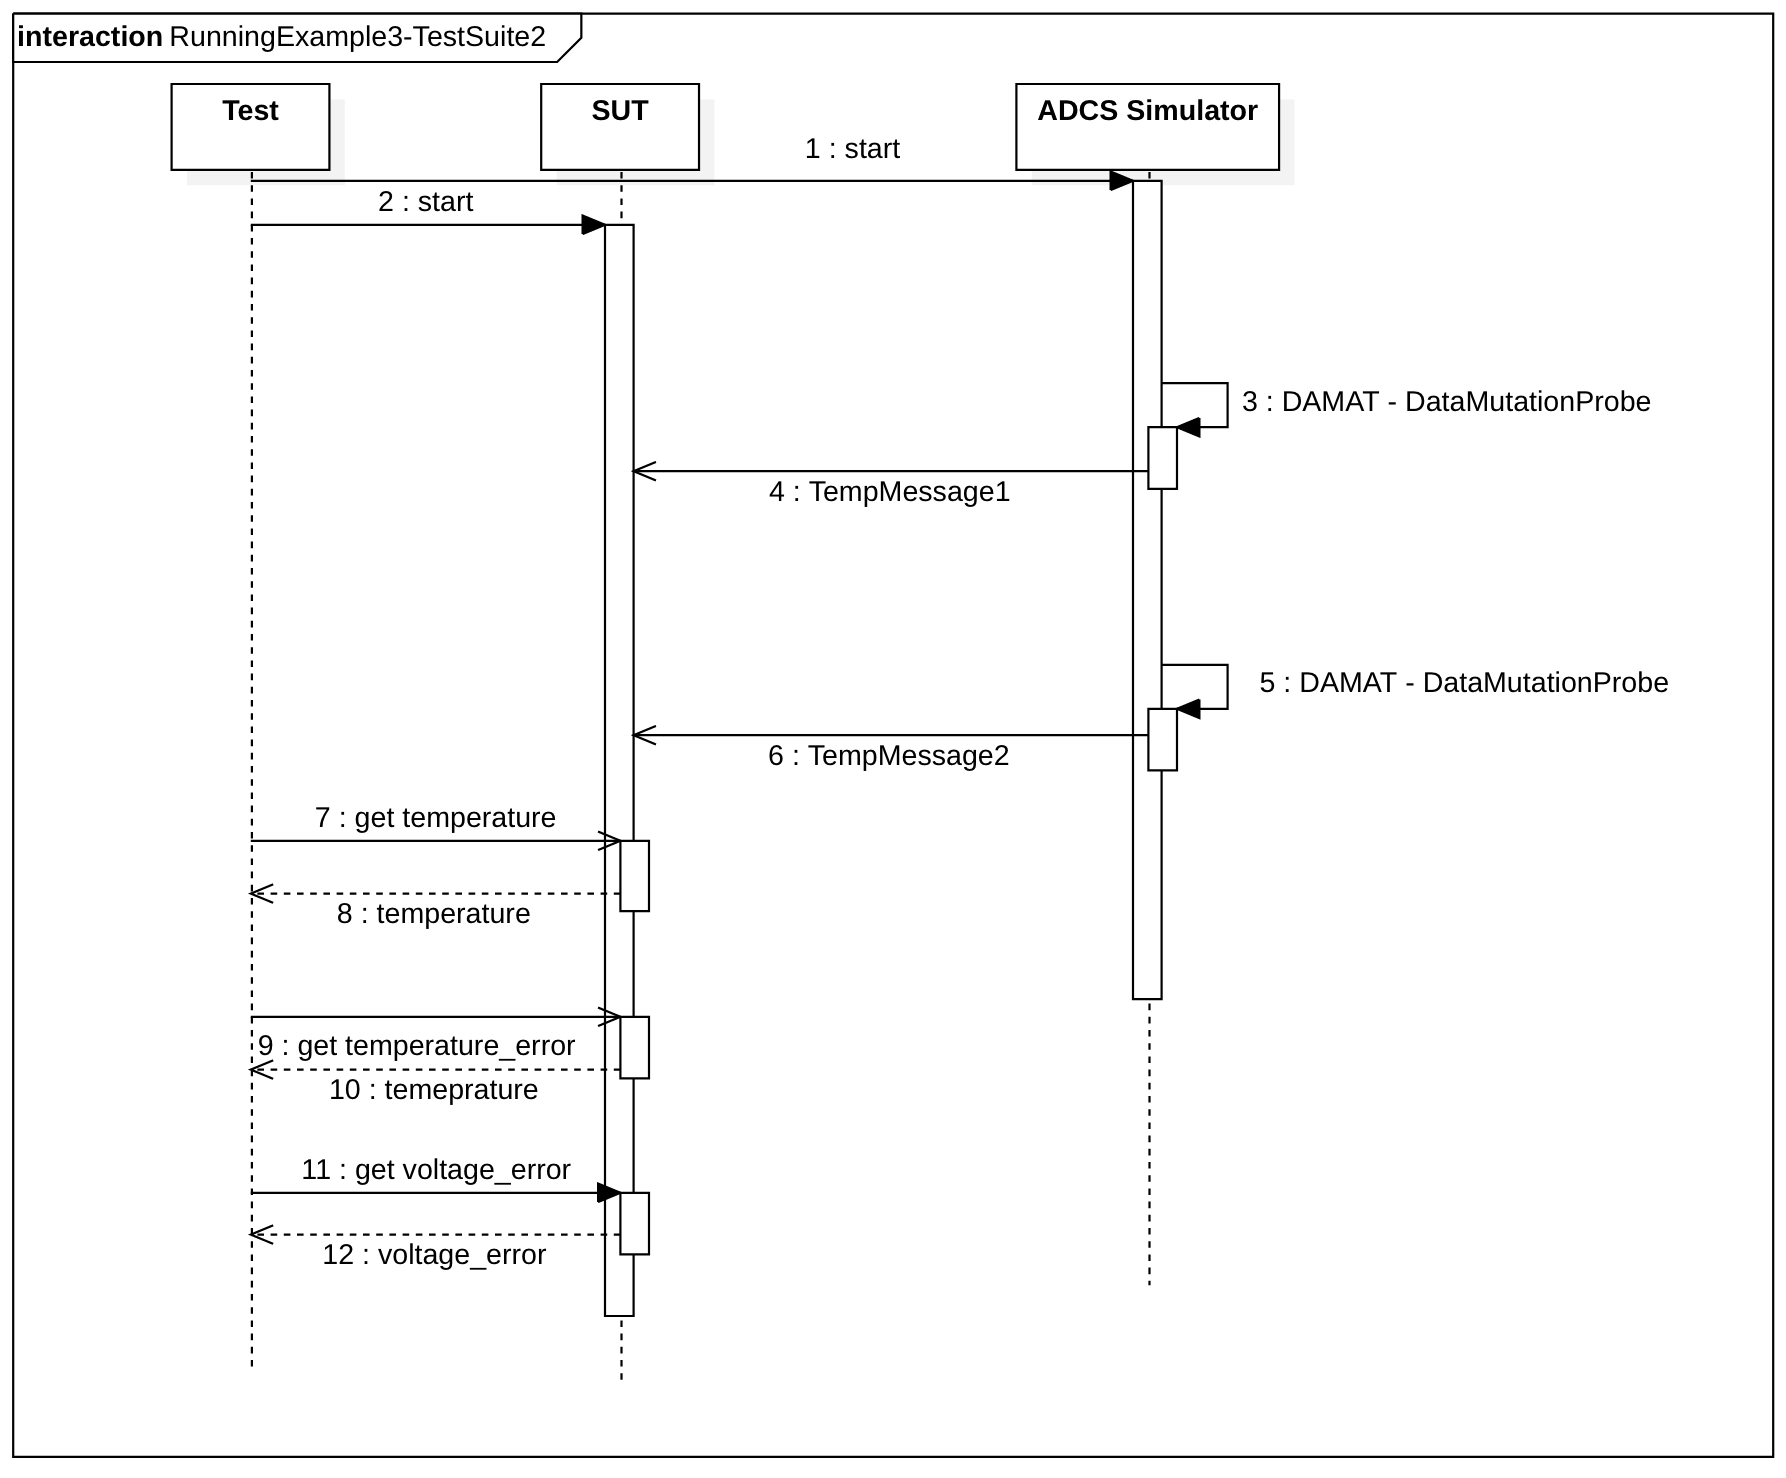
\includegraphics[width=8cm]{damat/images/runningExamplesSequence3_2.png}
\caption{Interactions exercised by the test cases of TestSuite2 in the running example set 3.}
\label{fig:damat:RunningExample3Sequence2}
\end{figure}

TestSuite 2 does not trigger messages of type BoardStatus; its interactions are depicted in Figure~\ref{fig:damat:RunningExample3Sequence2}. For the remaining message type (i.e., TempMessage) it covers all the possible combinations of temperature alarms being present/absent for two TempMessages sent in sequence; in total, we have 4 test cases.

The fault model BoardStatus is not covered; therefore the fault model coverage (FMC) is 50\%. Since MUTANTS 3 to 6 belong to BoardStatus they are not considered in the computation of the other mutation analysis metrics. MOC and MS are thus 100\%; indeed all the mutants not belonging to BoardStatus are killed by the test suite.

MUTANT 1 could be live only if relevant oracles are missing; more precisely, only if oracles concerning the nominal temperature value are missing. MUTANT 1 is killed by TestSuite2.

MUTANT 2 could be live only if relevant oracles are missing; indeed, only if oracles concerning the non nominal temperature value are missing. MUTANT 2 is killed by TestSuite2.
% !TEX root = MAIN.tex




\section{Data-driven Mutation Testing: DAMTE} % (fold)
\label{sec:data:test_suite_augmentation}



The \INDEX{test suite augmentation process} it consists of four activities \INDEX{Identify Test Inputs}, \INDEX{Generate Test Oracles}, \INDEX{Execute the SUT}, \INDEX{Fix the SUT}. It has the objective of increasing the score generated by the mutation analysis process.

FAQAS focussed on a methodology (i.e., data-driven mutation testing, \INDEX{DAMTE}) that specifies how to rely on KLEE to generate test inputs that increase the fault model coverage and the mutation operation coverage.
FAQAS does not address increasing the mutation score because infeasible in automated manner.
We recall that two might be the reasons for a low MS: poor oracle quality and missing test input sequences.
If the low mutation score is due to poor oracle quality, manual work is needed because automated approaches to automatically generate test oracles in the presence of system or integration test suites are not available. 
If the low mutation score is due to missing test input sequences (i.e., the software does not reach the state in which it could kill the mutant), manual work is required because existing test generation approaches (e.g., KLEE) might suffer from scalability problem that prevent bringing the system into a desired state; also, they cannot deal with systems whose components communicate through channels. 

For the cases targeted by FAQAS (i.e.,
in the presence of fault model coverage and mutation operation coverage below 100\%), test generation has the objective of generating test inputs that enable the application of all the mutation operators. 
We thus rely on an  \INDEX{extended data mutation probe} that
invokes a version of the data mutation API that instead of mutating the data targeted by the mutation operator not covered by the fault model, includes a reachability assertion that is used to make KLEE find a test input that reaches the mutant code. The test input shall then be inspected by the engineer, who will need then to integrate it into his test suite.
%Figure~\ref{fig:dataDrivenTestSuiteAugmentationB} exemplifies how data driven mutation testing works, for the producer consumer and client-server cases.
%
%
%
%
%\begin{figure}[h]
%  \centering
%    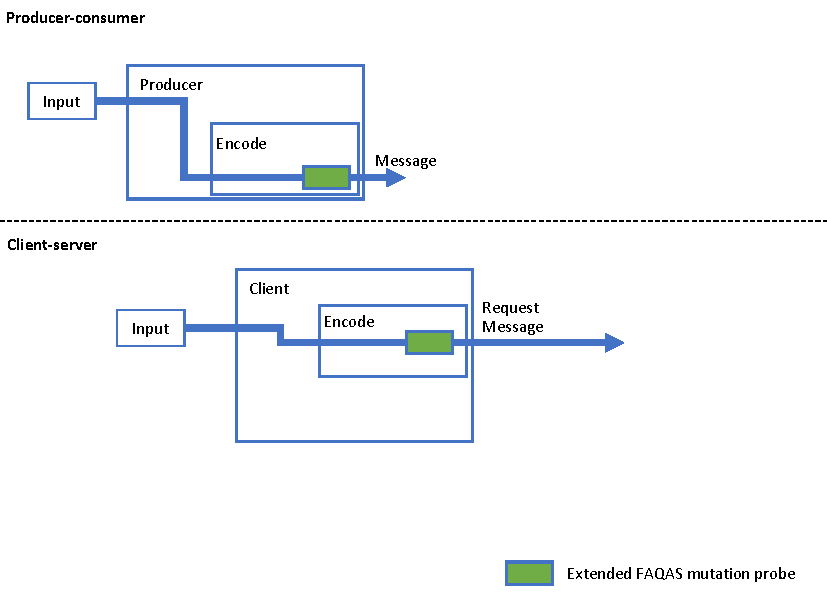
\includegraphics[width=14cm]{images/dataDrivenTestSuiteAugmentationB}
%      \caption{Data-driven mutation analysis for different architectures.}
%      \label{fig:dataDrivenTestSuiteAugmentationB}
%\end{figure}









% !TEX root = MAIN.tex

\chapter{FAQAS case studies}
\label{chapter:caseStudies}

The FAQAS toolset has been applied to \MREVISION{C-P-40}{six} case study systems. Table~\ref{tab:caseStudies} provides the list of case studies along with an indication of the type of mutation analysis/testing (i.e., code-driven or data-driven) and the tools they are targeted for. 

\STARTCHANGEDWPT
For the validation of each tool, we selected case studies presenting characteristics compatible with the requirements of the tool under test. \emph{Code-driven mutation analysis} (implemented by MASS) does not present any specific requirement except the availability of source code; for this reason, it has been validated with all the available case studies systems.
\emph{Code-driven mutation testing} (implemented by SEMuS), instead, requires the software under test to be comprised of components communicating through function calls (e.g., not network channels); for this reason, for SEMuS, we selected unit test suites.
\emph{Data-driven mutation analysis} (implemented by DAMAt) targets components communicating through channels, which are usually tested with integration and system test suites. For this reason we selected systems tested with such types of test suites.
\emph{Data-driven mutation testing} (implemented by DAMTE) aims to generate test cases that improve data-driven mutation analysis; however, since it is performed with symbolic execution tools, it presents the same limitations of SEMuS, that is, the analyzed part of the software under test should be comprised of components communicating through function calls. For this reason, it can target only libGCSP and libParam.

The following sections describe each case study subject. 

\begin{table}[htp]
\caption{Case studies for the FAQAS activity.}
\label{tab:caseStudies}
\begin{center}
\begin{tabular}{|p{1.2cm}|p{6cm}|p{1.5cm}|p{1.5cm}|p{1.5cm}|p{1.5cm}|}
\hline
\textbf{}&\textbf{}&\multicolumn{2}{c}{\textbf{Code-driven}}&\multicolumn{2}{c|}{\textbf{Data-driven}}\\
\textbf{Partner}&\textbf{Case study}&\textbf{MASS}&\textbf{SEMuS}&\textbf{DAMAt}&\textbf{DaMTe}\\
\hline
LXS&System Test Suite for ESAIL&Y&N&Y&N\\
LXS&Unit Test Suite for ESAIL&Y&N&N&N\\
GSL&Unit Test Suite for libUtil&Y&Y*&N&N\\
GSL&Integration Test Suite for libgscsp&Y&N&Y*&N\\
GSL&System Test Suite for libparam&Y&N&Y&Y*\\
ESA&MLFS mathematical library&Y&Y&N&N\\
ESA&ASN1 Compiler&Y&Y&N&N\\
\hline
\end{tabular}
\end{center}
An asterisk (*) is used to indicate validation cases that will be finalized in WP4.
\end{table}

\ENDCHANGEDWPT

\clearpage

% !TEX root = MAIN.tex

\section{LXS - ESAIL System Test Suite}
\label{chapter:caseStudies:LXS}

\subsection{Overview of the case study}

ESAIL is a microsatellite developed by LXS in a PPP with ESA and ExactEarth. 
The Payload is an AIS Receiver for ship- and vessel-detection from space, and the satellite weight at launch will be approximately 115kg. The satellite payload also enables advanced raw data handling and RF-Spectrum sampling for Ground processing.

\begin{figure}[h]
	\centering
    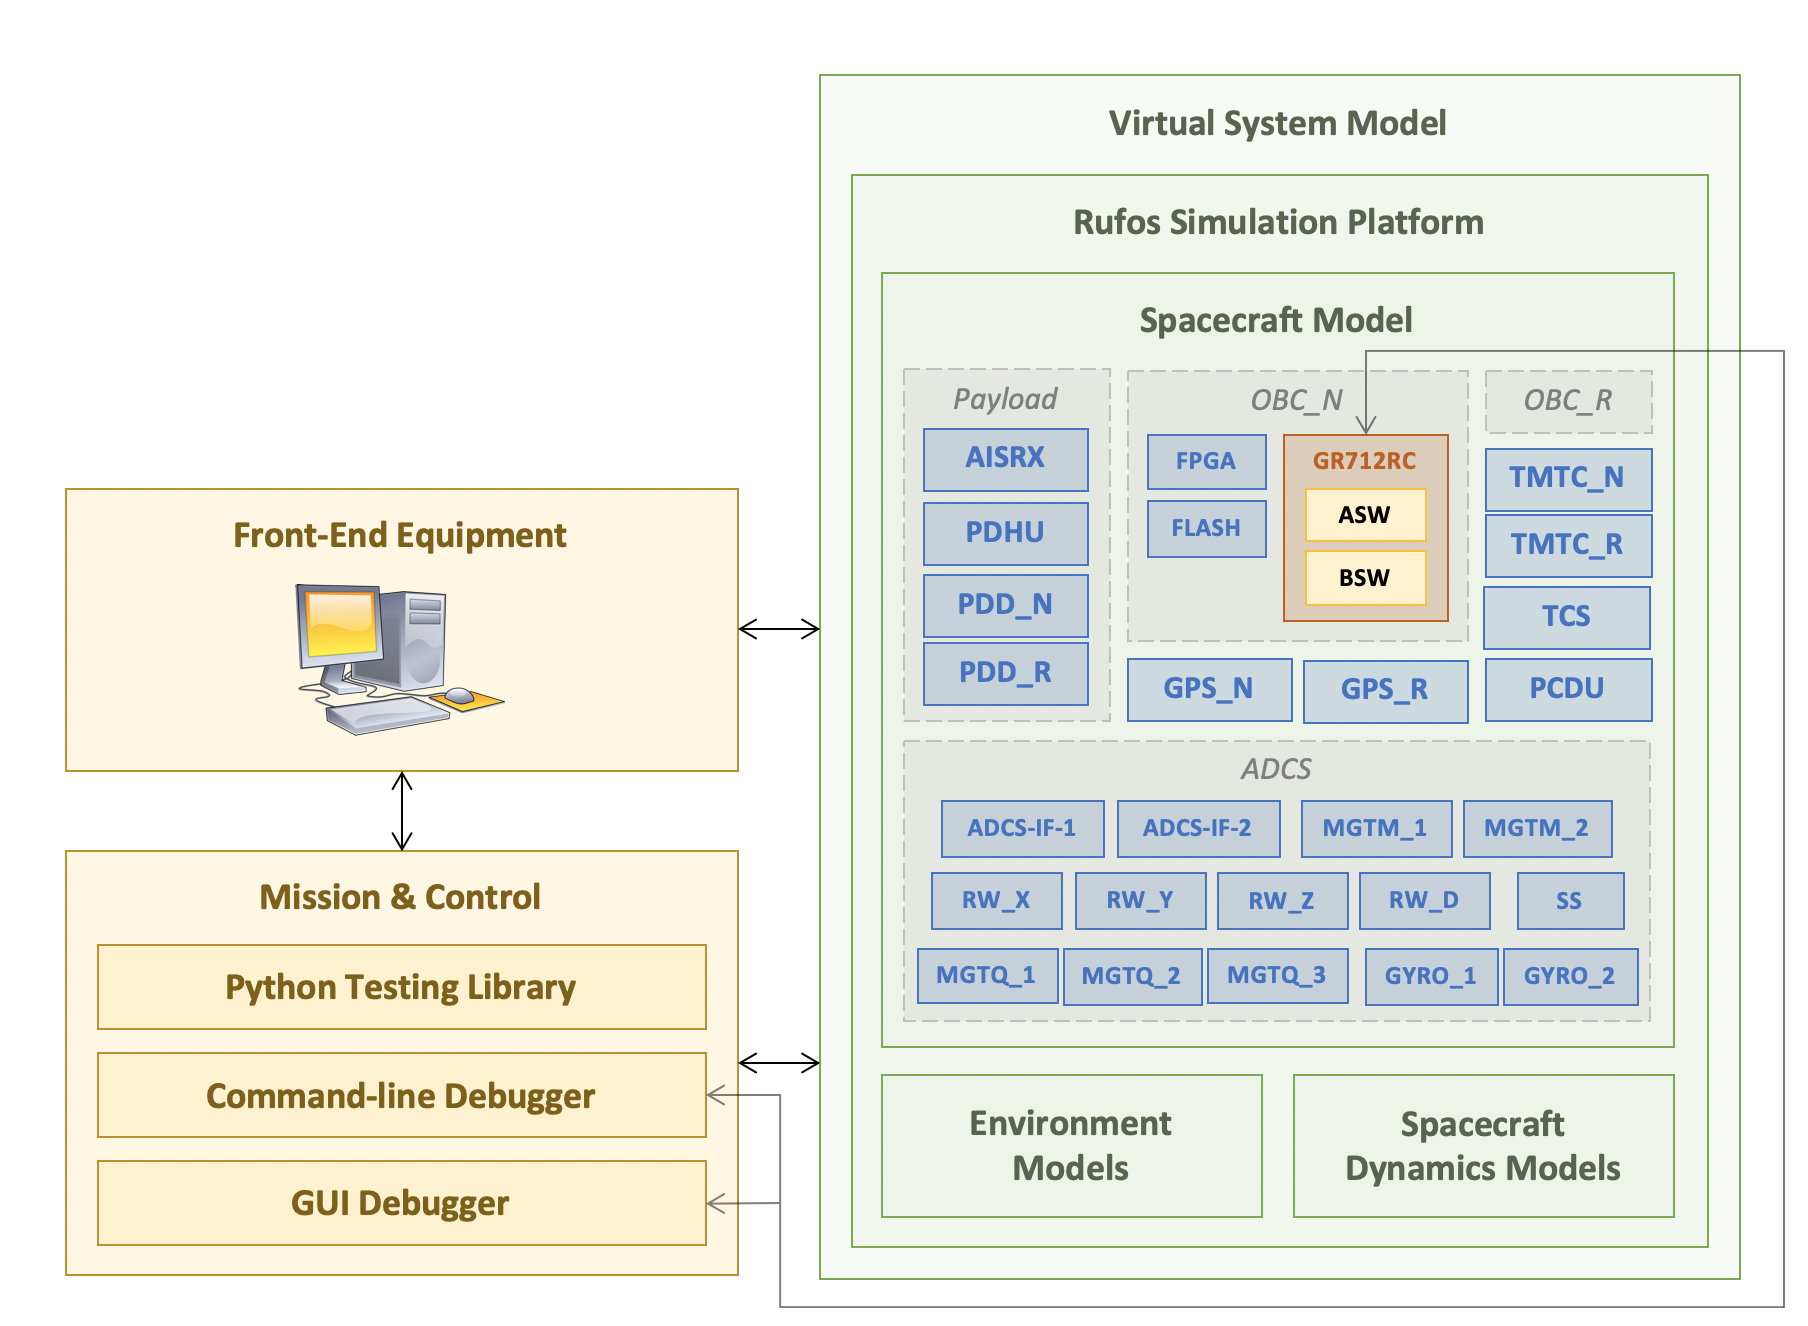
\includegraphics[width=0.7\textwidth]{images/esail}
    \caption{ESAIL system testing environment.}
    \label{fig:esail_case_study}
\end{figure}
 
The SVF simulator has been used for functional validation of the ESAIL CSW (see Figure~\ref{fig:esail_case_study}). The SVF is indeed one of the main testing tools used in satellite projects. The SVF simulator can be seen as a testing facility that presents also its own dedicated test suite to ensure the correctness of the SVF models and assembly to avoid later misunderstanding of the expected behaviours of the satellite CSW. 
In the context of the FAQAS project we consider the system test suite for the validation of the CSW, which are implemented using the SVF as the driving tool.
%Therefore, the SVF Simulator enables the evaluation of the FAQAS framework against two test suites: (1) the Test Suite of the SVF Simulator that validates the Simulator itself, (2) the system tests for the validation of CSW, which are implemented using the SVF as the driving tool.

Details about ESAIL are provided in the document \emph{FAQAS-LXS-MAN-001\_1- SVF Software Installation and User Manual} uploaded on Alfresco.

ESAIL is the largest case study system in FAQAS, the software consists of 924 source files with a total size of 187\,116 LOC. The system test suite consists of 121 python test scripts with a total of 384 sub-test cases. 
\MREVISION{C-P-22}{The system test suite takes up to 10 hours to finish its execution; the total execution time may be different and depends on the processing power of the computer where the SVF is being executed.}

\subsubsection{ESAIL System Test Suite Environment}

Because of the objectives of the project, we will need to execute a large number of mutants. Even if strategies for simplifying and reducing the number of mutants are designed (see Section~\ref{sec:approach}), there is a need for an infrastructure for running several mutant executions on parallel, which particularly applies for the ESAIL System Test Suite (e.g., the test suite execution time is high).

The University of Luxembourg provides a High-Performance Computing platform for academic purposes\footnote{https://hpc.uni.lu}.
The HPC has a computing capacity of 690 nodes, totaling 11\,280 computing cores, and a storage capacity of 8\,742 TB.

Given that ESAIL runs on a simulator (i.e., SVF), which is compute-intensive, and that resources of the UL HPC are shared between multiple jobs, non-deterministic behaviors are seldom observed (e.g., test cases fail because of lack of resources).

In view of the code-driven mutation testing process, where the quality of a test suite is assessed by checking if an injected fault is detected by the existing test cases, we need a test suite with a deterministic behavior, that is, if a test case fails it exclusively depends if we have introduced an artificial fault (i.e., a code mutation), and not because of the running environment.

To ensure that a mutant has been actually killed when executing the ESAIL System Suite on the UL HPC, we propose to execute a test case up to 10 times. If for any of this 10 executions the mutant is not killed, we consider it a live mutant. Otherwise, if it fails 10 times, we consider it a killed mutant.


Detailed information about the ESAIL system is provided in the following documents shared on Alfresco:

\begin{itemize}
	\item \emph{FAQAS-LXS-MAN-001\_1- SVF Software Installation and User Manual.pdf}, installation and testing instructions of the virtual machine containing ESAIL
	\item \emph{ESAIL-LXS-SDD-P-0105\_1B On-board Application Software Design Document.docx}, specifications document for the on-board system.
	\item \emph{ESAIL-LXS-ICD-P-0184\_2A ADCS IF SW External ICD.docx}, specifications document for the ADCS software.
	\item \emph{MOC-applicable MIB egos-mcs-s2k-icd-0001-version7.0-FINAL.pdf},  interface control document of the data import into SCOS-2000 run-time database, which is used to specify  the nominal value ranges for ESAIL ADCS parameters.
	\item \emph{ocp.dat}, text file for the SCOS-2000 Database Import ICD, containing the specifications of the nominal value ranges for ESAIL ADCS parameters.
\end{itemize}	


\subsection{Code-driven mutation testing}
\label{lxs:esail:system:codeDriven}

%\TODO{Code coverage information: we need Yago to produce a new code coverage report with VCAST.}

\REVNOV{PTCR-34}{The code-driven mutation testing process in ESAIL will be performed in two stages. First we will use a subset of ESAIL ($\mathit{ESAIL}_S$) to evaluate the accuracy of the estimated mutation score (see Section~\ref{sec:evaluation}). Then, in later stages, we will apply the approach (including mutants sampling, which is necessary for scalability purposes) to the whole ESAIL in order to (1) compare the mutation score obtained with the whole system with the mutation score obtained with $\mathit{ESAIL}_S$, (2) evaluate the accuracy of our strategy for removing equivalent/redundant mutants when applied to the whole ESAIL, (3) compare the mutation score obtained for the whole $ESAIL$ and for $\mathit{ESAIL}_S$ after removing likely equivalent and likely redundant mutants.}

\REVNOV{PTCR-34}{$\mathit{ESAIL}_S$ had been selected by LXS engineers by identifying representative source files that belong to the following categories: (1) source files that are used almost all the time by the test cases (i.e., files implementing service/protocol layer functions), (2) critical functions of the satellite implemented in high-level drivers, (3)  higher level application level functions.}

\STARTCHANGEDNOV
The files included in $\mathit{ESAIL}_S$ are:
\begin{itemize}
\item \emph{HighLevelDriverLayer/TMTC\_SYS\_Handler/Source/tmtchdl\_TmTcSysHandlerTask.c}
\item \emph{ProtocolLayer/TCFrameReader/Source/TCFrameReader.c}
\item \emph{ProtocolLayer/TMFrameBuilder/Source/TMFrameBuilder.c}
\item \emph{ServiceLayer/PUS\_1/Source/pus1\_GenerateReport.c}
\item \emph{ServiceLayer/PUS\_3/Source/pus3\_GenerateHkGroupReport.c}
\item \emph{ServiceLayer/PUS\_3/Source/pus3\_ExecuteTc\_3\_129.c}
\item \emph{ServiceLayer/PUS\_128/Source/pus128\_ExecuteTc\_128\_1.c}
\item \emph{ServiceLayer/PUS\_130/Source/pus130\_ExecuteTc\_130\_1.c}
\item \emph{ApplicationLayer/Operational\_Sequences/Source/SpacecraftConfigurationVector.c}
\item \emph{ApplicationLayer/Operational\_Sequences/Source/Transition\_To\_OPM.c}
\end{itemize}
\ENDCHANGEDNOV

Concerning the experiments conducted on the whole ESAIL, they will target all the components of the ESAIL on-board software, these components are:

\begin{itemize}
	\item ADCS
	\item CAN
	\item EPS
	\item FDIR
	\item OPSE
	\item SERVICES
	\item TCS
	\item TMTC
\end{itemize}

Code coverage information concerning the system-level test suite used for FAQAS is reported in \emph{FAQAS-LXS-MAN-001\_1- SVF Software Installation and User Manual.pdf}.


\subsection{Data-driven mutation testing}

A detailed description of the application of data-driven mutation testing to ESAIL is provided in APPENDIX~\ref{appendix:FMS}.

\section{LXS - ESAIL Unit Test Suite}
\label{chapter:caseStudies:LXS:Unit}



The unit test suite of ESAIL will be considered for the evaluation of the final FAQAS toolset. 
%For example, it is a possible case to be used for an independent use of the FAQAS framework by LXS engineers. The ESAIL unit test suite is used mainly to test critical functionalities of ESAIL components. The ESAIL unit test suite has been provided to ESA; however, the mutation testing activity might concern a subset of them. Indeed, evaluating with mutation testing a set of test cases that are known for covering only a subset of the features of the system might be of little usefulness. 
%%The set of test cases and functions to be tested will be provided along with the description of the achieved results at the end of WP3.
To assess the quality of the ESAIL unit test suite we will analyze the same ESAIL sub-system defined in Section~\ref{lxs:esail:system:codeDriven}, and thus, we will target the same set of mutants. Since the ESAIL Unit Test Suite has been implemented by LXS to cover scenarios hard to cover with a full simulation (consequently, it cover a limited portion of the code), we will use the ESAIL Unit Test Suite to provide a complementary analysis to the one given by the system test suite.



% !TEX root = MAIN.tex

\clearpage

\section{GSL - libgcsp}
\label{sec:caseStudies:GSL:libgcsp}

\subsection{Overview of the case study}

The GomSpace CSP library (libgscsp) is a GomSpace extension to the open source CubeSat Space Protocol library.
The GomSpace CSP library provides:
\begin{itemize}
\item convenience wrapping of CSP functionality, primarily initialization.
\item definition of standard CSP ports (used by other GomSpace products).
\item connecting low-level drivers (e.g. CAN, I2C from Embed library) with CSP interfaces 
\item generic CSP service dispatcher, forwards incoming connections to service handlers.
\end{itemize}

The libgscsp contains a GomSpace branch (https://github.com/GomSpace/libcsp) of the open source libcsp (https://github.com/libcsp/libcsp), located in the subfolder lib/libcsp. The two libcsp branches are kept as identical as possible, as features specific to GomSpace are placed in libgscsp.

Details about libgscsp are provided in the document \emph{gs-man-nanosoft-ms100-command-and-management-sdk-3.6.2-1-g67fe6e1.pdf} uploaded on Alfresco.


The size of libgscsp is 1\,497 LOC, %include 306, src 1776+15 = total = 1497
while libcsp (GSL branch) is 8\,339 LOC. % 6789 + 1550
Instead, the libgscsp unit test suite consists of 89 test cases, compiled and executed through the WAF meta-build system.

\subsection{Code-driven mutation testing}

\DONE{Can we provide separate information about the code coverage for libgscsp (no libcsp branch) and for libcsp branch?}

\DONE{Clarify which components we mutate}

We have seen that a mutant can be killed only if it is covered by at least one test case. For this reason, the code-driven mutation testing process in libgscsp will target all the components covered by the libgscsp unit test suite.

% !TEX root = ../MAIN.tex

\begin{table}[h]

\footnotesize
\parbox{.45\linewidth}{
\centering
\begin{tabular}{|l|l|}
\hline
\textbf{Coverage Type} & \textbf{Coverage Rate} \\
\hline
Statement     & 58.4\% (390 of 668 statements)\\
Functions     & 71.4\% (50 of 70 functions)\\
Branches      & 41.2\% (165 of 400 branches)\\
\hline
\end{tabular}
\caption{libgscsp code coverage.}
\label{table:libgscsp_coverage}
}
\hfill
\parbox{.45\linewidth}{
\centering
\begin{tabular}{|l|l|}
\hline
\textbf{Coverage Type} & \textbf{Coverage Rate} \\
\hline
Statement     & 64.1\% (2112 of 3297 statements)\\
Functions     & 72.5\% (248 of 342 functions)\\
Branches      & 44.9\% (989 of 2201 branches)\\
\hline
\end{tabular}
\caption{libcsp code coverage.}
\label{table:libcsp_coverage}
}
\end{table}	

\begin{enumerate}
	\item \textbf{libgscsp}

	Table~\ref{table:libgscsp_coverage} provides code coverage information of the libgscsp unit test suite for the GSL extension to the CSP library. Given the code coverage, we focus our analysis to the following subset of components (i.e., components with code coverage greater than 0\%):

	\begin{itemize}
	 	\item src/clock.c
	 	\item src/commands.c
	 	\item src/conn.c
	 	\item src/csp.c
	 	\item src/error.c
	 	\item src/log.c
	 	\item src/router.c
	 	\item src/service\_dispatcher.c
	 	\item src/service\_handler.c
	 	\item src/linux/command\_line.c

	 \end{itemize} 

	\item \textbf{libcsp (GSL branch)}

	Table~\ref{table:libcsp_coverage} presents the code coverage of the libgscsp unit test suite for the GSL branch of the CSP library.  Given the code coverage, we focus our mutation analysis on the following subset of components (i.e., components with code coverage greater than 0\%):

	\begin{itemize}
		\item src/arch/csp\_time.c
		\item src/arch/csp\_system.c
		\item src/arch/posix/csp\_thread.c
		\item src/arch/posix/csp\_semaphore.c
		\item src/arch/posix/csp\_malloc.c
		\item src/arch/posix/csp\_queue.c
		\item src/arch/posix/csp\_time.c
		\item src/arch/posix/pthread\_queue.c
		\item src/arch/posix/csp\_system.c
		\item src/crypto/csp\_sha1.c
		\item src/crypto/csp\_hmac.c
		\item src/crypto/csp\_xtea.c
		\item src/interfaces/csp\_if\_lo.c
		\item src/rtable/csp\_rtable.c
		\item src/rtable/csp\_rtable\_cidr.c
		\item src/rtable/csp\_rtable\_static.c
		\item src/transport/csp\_rdp.c
		\item src/transport/csp\_udp.c
		\item src/csp\_sfp.c
		\item src/csp\_debug.c
		\item src/csp\_service\_handler.c
		\item src/csp\_crc32.c
		\item src/csp\_io.c
		\item src/csp\_qfifo.c
		\item src/csp\_iflist.c
		\item src/csp\_endian.c
		\item src/csp\_route.c
		\item src/csp\_buffer.c
		\item src/csp\_port.c
		\item src/csp\_conn.c
		\item src/csp\_init.c
		\item src/csp\_services.c
	\end{itemize}


\end{enumerate}

\subsubsection{Mutation Testing Preliminary Results}

\DONE{We can add some preliminary results}

% !TEX root = ../MAIN.tex

\begin{table}[h]
\small
\centering
\caption{Code-driven mutation testing preliminary results for the libgscsp case study.}
\label{table:libgscsp_preliminary}
\begin{tabular}{|l|l|l|l|l|l|l|}
\hline
        & \multicolumn{5}{c|}{Mutants}                                                                      & \multirow{3}{*}{\begin{tabular}[c]{@{}l@{}}Mutation Score\\ (K/K+L)\end{tabular}} \\ \cline{1-6}
        &     &                                                        &      & \multicolumn{2}{c|}{Killed} &                                                                                   \\ \cline{1-6}
Mutants & All & \begin{tabular}[c]{@{}l@{}}Not\\ Compiled\end{tabular} & Live & Test Failure    & Timeout   &                                                                                   \\ \hline
Total   &  6\,196   &  1\,700 & 1\,708      & 2\,495                & 277          & 61.88\%                                                                           \\ \hline
\end{tabular}
\end{table}    
             

In order to analyze the feasibility of the code-driven mutation testing for libgscsp, we conducted a preliminary experimentation using the mutation operators AOR, ROR, ICR, LCR, ABS, UOI and SDL we generated 6\,196 mutants. For the experimentation we consider only the libcsp (GSL branch) source code. Preliminary results can be found in Table~\ref{table:libgscsp_preliminary}.
Particularly, we observe that from the 6\,196 generated mutants, we had 1\,700 mutants that were not compiled by the compilation toolset of libgscsp, most probably because the mutation introduced a syntactical error that was detected by the toolset.
Then, we identified 1\,708 live mutants that were not detected by the test suite. Instead, we had 2\,495 killed mutants detected by the test suite, and 277 mutants that produced libutil to go into an infinite loop, and thus were killed by timeout. The final mutation score was of 61.88\%.

The identification of equivalent mutants still needs to be assessed.


\subsection{Data-driven mutation testing}

\DONE{We should indicate the functions we mutate.}

The data-driven mutation testing process in libgscsp will target the data packet transferred between the server and the client using the CSP protocol. Specifically, the mutations will affect the header of the packet, in general the routing information (see Figure~\ref{fig:csp_packet}), and the payload of the packet.

\begin{figure}[h]
  \centering
    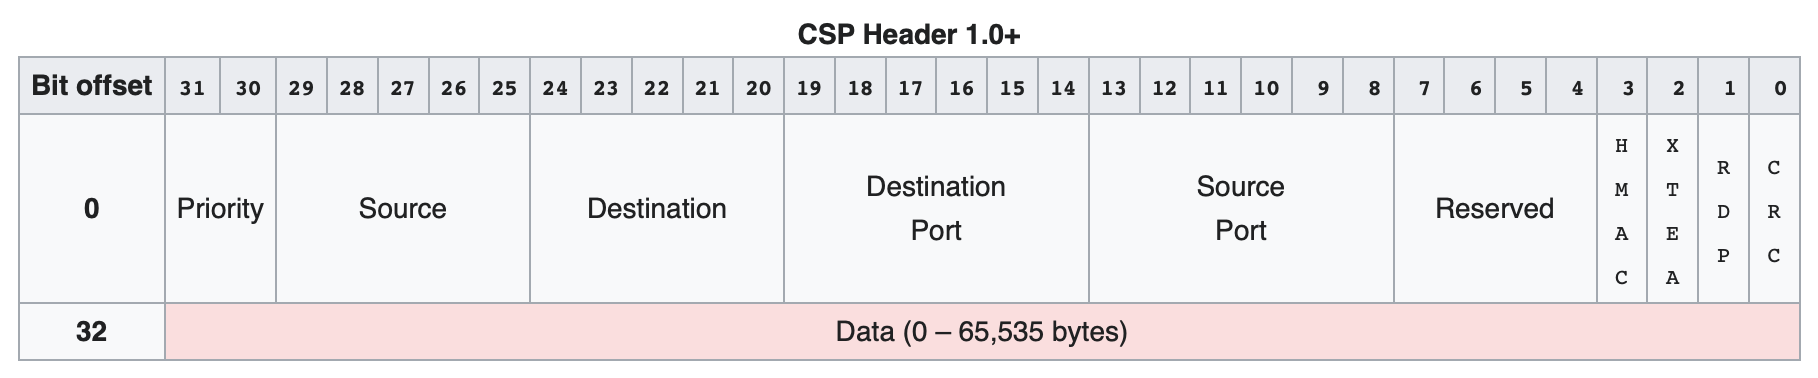
\includegraphics[width=0.9\textwidth]{images/csp_packet}
      \caption{CSP protocol header.}
      \label{fig:csp_packet}
\end{figure}


% !TEX root =  ../MAIN.tex

\begin{minipage}{16cm}
\begin{lstlisting}[style=CStyle, caption=Data-driven mutation example on libgscsp (csp\_io.c excerpt)., label=csp_integration]
unsigned int v[6] = {packet->id.flags, packet->id.sport, packet->id.dport, 
                    packet->id.dst, packet->id.src, packet->id.pri};

FaultModel *fm = _FAQAS_Identifier_FM();                                                                                          
mutate(v, fm);
_FAQAS_delete_FM(fm);

packet->id.flags = v[0];
packet->id.sport = v[1];
packet->id.dport = v[2]; 
packet->id.dst = v[3]; 
packet->id.src = v[4]; 
packet->id.pri = v[5]; 
\end{lstlisting}
\end{minipage}


Both mutations (i.e, header and payload) will be performed before the message is serialized. 
For example, the mutations to the header will affect the csp\_send\_direct function of the csp\_io component. Listing~\ref{csp_integration} shows an example of our data-driven mutator prototype within the csp\_io component. Particularly, the packet header is translated into an unsigned int vector, which is then passed to the FAQAS mutate function, here a fault model could be applied to all six items of the header. After the mutation is applied the vector is translated back again to the original representation.
 

\section{GSL - libparam}
\label{sec:caseStudies:GSL:libparam}

\subsection{Overview of the case study}

The Parameter System (i.e., libparam) is a light-weight parameter system designed for GomSpace satellite subsystems. It is based around a logical memory architecture, where every parameter is referenced directly by its logical address. A backend system takes care of translating addresses into physical addresses.
The features of this system include:
\begin{itemize}
\item Direct memory access for quick parameter reads.
\item Simple data types: uint, int, float, double, string.
\item Arrays of simple data types.
\item Supports multiple stores per table, e.g. FRAM, MCU flash, file (binary or text).
\item Remote client with support for most features (rparam).
\item Packed GET, SET queries, supporting multiple parameter set/get in a single request. Data serialization and deserialization.
\item Supports both little and big-endian systems.
\item Commands for both local (param) and remote access (rparam).
\item Parameter server for remote access over CSP.
\item Compile-time configuration of parameter system
\end{itemize}

Details about libparam are provided in the document \emph{gs-man-nanosoft-ms100-command-and-management-sdk-3.6.2-1-g67fe6e1.pdf} uploaded on Alfresco.

\subsection{Code-driven mutation testing}

\TODO{We do it or not?}

\subsection{Data-driven mutation testing}

\TODO{We should indicate the functions we mutate}


\section{GSL - libutil}
\label{sec:caseStudies:GSL:libutil}

\subsection{Overview of the case study}

The Utility library provides cross-platform APIs for common functionality, for use in both embedded systems and standard PCs running Linux. 

Details about libutil are provided in the document \emph{gs-man-nanosoft-ms100-command-and-management-sdk-3.6.2-1-g67fe6e1.pdf} uploaded on Alfresco.

The size of libutil is 10\,576 LOC, while the unit test suite consists of 201 test cases written in C.

\subsection{Code-driven mutation testing}

\DONE{Add some details about what we mutated}

The code-driven mutation testing process in libutil will target all the components covered by the libutil unit test suite. 

% !TEX root = ../MAIN.tex

\begin{table}[h]

\centering
\begin{tabular}{|l|l|}
\hline
\textbf{Coverage Type} & \textbf{Coverage Rate} \\
\hline
Statement     & 83.2\% (8\,817 of 10\,596 statements)\\
Functions     & 82.1\% (725 of 883 functions)\\
Branches      & 56.6\% (2\,618 of 4\,627 branches)\\
\hline
\end{tabular}
\caption{libutil code coverage.}
\label{table:gslibutil_coverage}

\end{table}

Table~\ref{table:gslibutil_coverage} provides the code coverage information of the unit test suite for the GSL libutil library. Given the code coverage, we focus our analysis to the following subset of components (i.e., components with code coverage greater than 0\%):

\begin{itemize}
	\item src/base16.c
	\item src/bytebuffer.c
	\item src/byteorder.c
	\item src/clock.c
	\item src/crc32.c
	\item src/crc8.c
	\item src/error.c
	\item src/fletcher.c
	\item src/function\_scheduler.c
	\item src/hexdump.c
	\item src/lock.c
	\item src/rtc.c
	\item src/string.c
	\item src/strtoint.c
	\item src/time.c
	\item src/timestamp.c
	\item src/cmd/command.c
	\item src/cmd/log.c
	\item src/cmd/vmem.c
	\item src/drivers/sys/memory.c
	\item src/gosh/command.c
	\item src/gosh/console.c
	\item src/gosh/default\_commands.c
	\item src/linux/clock.c
	\item src/linux/command\_line.c
	\item src/linux/cwd.c
	\item src/linux/delay.c
	\item src/linux/function.c
	\item src/linux/mutex.c
	\item src/linux/queue.c
	\item src/linux/rtc.c
	\item src/linux/sem.c
	\item src/linux/signal.c
	\item src/linux/stdio.c
	\item src/linux/thread.c
	\item src/linux/time.c
	\item src/linux/drivers/gpio/gpio.c
	\item src/linux/drivers/gpio/gpio\_sysfs.c
	\item src/linux/drivers/gpio/gpio\_virtual.c
	\item src/linux/drivers/i2c/i2c.c
	\item src/linux/drivers/spi/spi.c
	\item src/linux/drivers/sys/memory.c
	\item src/log/commands.c
	\item src/log/log.c
	\item src/log/appender/console.c
	\item src/log/appender/simple\_file.c
	\item src/test/cmocka.c
	\item src/test/command.c
	\item src/test/log.c
	\item src/vmem/commands.c
	\item src/vmem/vmem.c
	\item src/watchdog/monitor\_task.c
	\item src/watchdog/watchdog.c
	\item src/zip/zip.c
	\item src/zip/miniz/miniz.c
\end{itemize}

\subsubsection{Mutation Testing Preliminary Results}

\DONE{We can add some preliminary results}

% !TEX root = ../MAIN.tex

\begin{table}[h]
\small
\centering
\caption{Code-driven mutation testing preliminary results for the libutil case study.}
\label{table:libutil_preliminary}
\begin{tabular}{|l|l|l|l|l|l|l|}
\hline
        & \multicolumn{5}{c|}{Mutants}                                                                      & \multirow{3}{*}{\begin{tabular}[c]{@{}l@{}}Mutation Score\\ (K/K+L)\end{tabular}} \\ \cline{1-6}
        &     &                                                        &      & \multicolumn{2}{c|}{Killed} &                                                                                   \\ \cline{1-6}
Mutants & All & \begin{tabular}[c]{@{}l@{}}Not\\ Compiled\end{tabular} & Live & Test Failure    & Timeout   &                                                                                   \\ \hline
Total   &  16\,886   &  2\,561                                                      & 3\,402      & 10\,634                & 289          & 76.25\%                                                                           \\ \hline
\end{tabular}
\end{table}    
             

In order to analyze the feasibility of the code-driven mutation testing, we conducted a preliminary experimentation using the mutation operators AOR, ROR, ICR, LCR, and SDL we generated 16\,886 mutants. Preliminary results can be found in Table~\ref{table:libutil_preliminary}.
Particularly, we observe that from the 16\,886 generated mutants, we had 2\,561 mutants that were not compiled by the compilation toolset of libutil, most probably because the mutation introduced a syntactical error that was detected by the toolset.
Then, we identified 3\,402 live mutants that were not detected by the test suite. Instead, we had 10\,634 killed mutants detected by the test suite, and 289 mutants that produced libutil to go into an infinite loop, and thus were killed by timeout. The final mutation score was of 76.25\%.

The identification of equivalent mutants still needs to be assessed.


\subsection{Data-driven mutation testing}

We do not plan to apply data drive mutation testing to this case study because is a standalone library; it does not integrate communicating components.



% !TEX root = MAIN.tex
\clearpage

\section{MLFS}
\label{sec:caseStudies:GSL:MLSF}

\subsection{Overview of the case study}

The \INDEX{Mathematical Library for Flight Software} (MLFS) implements mathematical functions ready for qualification. 
%\DONE{Please rewrite the following sentence}
MLFS is born from the need of having a mathematical library ready for qualification for flight software. Well known mathematical libraries such as \texttt{libm}~\cite{libm} and \texttt{newlib}~\cite{newlib} are not completely validated with respect to specific input ranges, errors and performance, and so, they do not comply with ECSS criticality category B.
The set of functions provided by MLFS are limited to the functions typically needed in flight software. 


The source code size is 5\,402 LOC, while the unit test suite consists of 4\,042 tests for 92 functions.



% !TEX root = MAIN.tex

\clearpage

\section{ASN1SCC}
\label{sec:caseStudies:GSL:ASN1}

\subsection{Overview of the case study}

ASN1SCC is an open source ASN.1 compiler that generates C/C++ and SPARK/Ada code suitable for low resource environments such as space systems. Moreover, the compiler can produce a test harness that provides full statement coverage in the generated code, and therefore significantly improves its quality.

Details about ASN.1 compiler are provided in the document \emph{taste-documentation-current.pdf} uploaded on Alfresco.

In the context of FAQAS, we focus our analysis on the auto-generated source code by the ASN.1 compiler, rather than in ASN1SCC software itself.

For the definition of the ASN.1 compiler case study, we introduce the example of a specific grammar. An excerpt of such grammar is shown in Listing~\ref{asn_excerpt}. 
The excerpt of the grammar introduces the definition of six data types, each data type also specifies the expected constraint, for example, the data type \texttt{MyInt} is an INTEGER which can have values from 0 to 20. The full source code of the grammar can be found in the file \emph{test.asn} uploaded on Alfresco.

For the given grammar, the size of the auto-generated source code is 4\,338 LOC. While the unit test suite consists of 107 auto-generated test cases.

% !TEX root =  ../MAIN.tex

\begin{minipage}{15cm}
\begin{lstlisting}[style=CStyle, caption=Excerpt of the tested ASN1 grammar., label=asn_excerpt, mathescape=true]
MyInt ::= INTEGER (0 .. 20)

My2ndInt ::= MyInt ( 1 .. 18)

AType ::= SEQUENCE {
    blArray SEQUENCE (SIZE(10)) OF BOOLEAN
}

My2ndAType ::= AType

TypeNested ::= SEQUENCE {
    intVal  INTEGER(0..10),
    int2Val INTEGER(-10..10),
    int3Val MyInt (10..12),
    intArray    SEQUENCE (SIZE (10)) OF INTEGER (0..3),
    realArray   SEQUENCE (SIZE (10)) OF REAL (0.1 .. 3.14),
    octStrArray SEQUENCE (SIZE (10)) OF OCTET STRING (SIZE(1..10)),
    boolArray   SEQUENCE (SIZE (10)) OF T-BOOL,
    label   OCTET STRING (SIZE(10..40)),
    bAlpha  T-BOOL,
    bBeta   BOOLEAN,
    sString T-STRING,
    arr     T-ARR,
    arr2    T-ARR2
}

E ::= INTEGER (0..255|1299)(5)
\end{lstlisting}
\end{minipage}



\subsection{Code-driven mutation testing}

% !TEX root = ../MAIN.tex

\begin{table}[h]

\centering
\begin{tabular}{|l|l|}
\hline
\textbf{Coverage Type} & \textbf{Coverage Rate} \\
\hline
Statement     & 83.7\% (2\,718 of 3\,246 statements)\\
Functions     & 87.4\% (285 of 326 functions)\\
Branches      & 51.2\% (1\,233 of 2\,407 branches)\\
\hline
\end{tabular}
\caption{ASN.1 grammar code coverage.}
\label{table:asn1grammar_coverage}

\end{table}



The objective of this case study is to provide ASN1SCC engineers tangible evidence on how to improve the auto-generated test cases, by reporting detailed information of live mutants and possible candidates of new test cases. In this manner, the quality of test suites of embedded systems that includes the auto-generated source code from ASN.1, can also be improved.

Table~\ref{table:asn1grammar_coverage} provides the code coverage information of the auto-generated source code of the \emph{test.asn} grammar. Given the code coverage, we focus our code-driven mutation testing analysis to the following subset of components (i.e., components with code coverage greater than 0\%):

\begin{itemize}
	\item asn1crt\_encoding.c: implementation of the ASN.1 constraints encoding/decoding procedures.
	\item test.c: implementation of the grammar data types encoding/decoding procedures.
	\item test\_auto\_tcs.c: wrapper of the grammar data types encoding/decoding procedures used in the test cases.
\end{itemize}

\subsubsection{Mutation Testing Preliminary Results}

% !TEX root = ../MAIN.tex

\begin{table}[h]
\small
\centering
\caption{Code-driven mutation testing preliminary results for the ASN.1 case study.}
\label{table:asn1_preliminary}
\begin{tabular}{|l|l|l|l|l|l|l|}
\hline
        & \multicolumn{5}{c|}{Mutants}                                                                      & \multirow{3}{*}{\begin{tabular}[c]{@{}l@{}}Mutation Score\\ (K/K+L)\end{tabular}} \\ \cline{1-6}
        &     &                                                        &      & \multicolumn{2}{c|}{Killed} &                                                                                   \\ \cline{1-6}
Mutants & All & \begin{tabular}[c]{@{}l@{}}Not\\ Compiled\end{tabular} & Live & Test Failure    & Timeout   &                                                                                   \\ \hline
Total   &  9\,174   &  1\,215   & 4\,263      & 3\,009                & 687          & 53.56\%                                                                           \\ \hline
\end{tabular}
\end{table}    
             

In order to analyze the feasibility of the code-driven mutation testing for ASN.1, we conducted a preliminary experimentation using the mutation operators AOR, ROR, ICR, LCR, ABS, UOI and SDL we generated 9\,174 mutants. Preliminary results can be found in Table~\ref{table:asn1_preliminary}.
Particularly, we observe that from the 9\,174 generated mutants, we had 1\,215 mutants that were not compiled by the compilation toolset of ASN.1, most probably because the mutation introduced a syntactical error that was detected by the toolset.
Then, we identified 4\,263 live mutants that were not detected by the test suite. Instead, we had 3\,009 killed mutants detected by the test suite, and 687 mutants that produced libutil to go into an infinite loop, and thus were killed by timeout. The final mutation score was of 53.56\%.

The identification of equivalent mutants still needs to be performed.


\subsection{Data-driven mutation testing}

In the context of this project, we foresee two scenarios on how to apply the data-driven mutation testing approach to the ASN.1 case study system. 

\subsubsection{Scenario 1: Testing the ASN.1 Compiler}

The first scenario simply automates robustness testing for ASN.1; we aim to rely on the automatically generated configuration parameters for mutation operators to generate data values that do not respect such constraints. This enables to verify the capability of the ASN.1 code to verifies the constraints of the data types defined in ASN.1 grammars.





%In the first scenario, we focus on the robustness of the auto-generated test cases of an ASN.1 grammar through the ASN.1 compiler.
%Particularly, we aim to apply a fault model that enables different mutations on the data types automatically generated by the ASN.1 compiler. Consequently, for every data type defined in the ASN.1 grammar, we automatically generate a set of probes that stresses all the data types constraints, where each probe contains a single instance of the defined fault model.
%
%The full description of the fault model can be found in Section~\ref{subsub:asn1model}.

\subsubsection{Scenario 2: Testing Case Study Systems using ASN.1}

%The second scenario aims to stress test suites from software systems that uses the encoding and decoding procedures derived from the ASN.1 compiler.
%
%More details about each scenario is provided in the following.

In this second scenario, we aim to assess the adequacy of test suites from software systems that embed the decoding and decoding auto-generated source code from ASN.1 grammar through the ASN.1 compiler.

For this task, we will ask engineers to specify fault models to decide what mutation operator to apply for each data type defined in the ASN.1 grammar.
Additionally, the engineer will be asked to specify in the fault model the nominal ranges for each data type; after applying a specific mutation operator, we will assess if the existing test suite is able to detect the corresponding mutated value by killing the introduced mutant.

For this scenario, further discussions with ESA are required in order to identify case study systems using the ASN.1 compiler. 






% !TEX root = MAIN.tex

\chapter{Empirical Evaluation}

% !TEX root =  Main.tex


\section{Code-driven mutation analysis: MASS}

\subsection{Overview}
\label{sec:evaluation}

\renewcommand{\APPR}{\textit{MASS}\xspace}

\STARTCHANGEDNOV

Our empirical evaluation aims to assess the effectiveness of the techniques integrated into \INDEX{\APPR} to address scalability and pertinence problems (i.e., Steps 2, 4, 5, 6, 7, and 8 of \APPR). Our objectives include (RQ1) confirming, in our context, trivial compiler optimization results observed in related work (Step 4), (RQ2) identifying the most effective solution for mutants sampling (Step 5), (RQ3) comparing mutants generation strategies implemented by \APPR (Step 2), evaluating the (RQ4) accuracy and (RQ5) effectiveness of the strategies proposed  for test suite prioritization (Step 6), and (RQ6) evaluating the accuracy of the strategy for the identification of likely equivalent/duplicate mutants (Step 7). Finally, we aim to (RQ7) compare the mutation score computed by \APPR (Step 8) with the mutation score computed without \APPR optimizations.
\REVNOV{C-P-11}{The project will include continuous empirical evaluation sessions with the case study systems that aim to address the following research questions:}

%Our empirical evaluation aims to address the following research questions, in the context of embedded space software:

\begin{itemize}

    \item[RQ1] \JMRCHANGE{(Step 4)} What are the cost savings provided by compiler optimization techniques detecting equivalent and duplicate mutants?
    We wish to determine what is the percentage of mutants reported as being equivalent and duplicate by compiler optimization techniques. After accounting for the additional compilation time entailed by such techniques, we want to identify the optimal subset of compilation options to be used in Step 4 of \APPR.

    \item[RQ2] \JMRCHANGE{(Step 5)} Can a randomly selected subset of mutants be used to accurately estimate the mutation score obtained from the entire set of mutants? 
    \CHANGED{We attempt to evaluate four mutants sampling strategies: \INDEX{proportional uniform sampling}, \INDEX{proportional method-based sampling},  \INDEX{uniform fixed-size sampling}, and \INDEX{uniform FSCI sampling}. More precisely, we aim to determine the best configuration for each sampling strategy (i.e., sampling ratio, sample size, and confidence interval). Furthermore, we need to identify which strategy offers the best trade-off between the number of mutants to be tested and accuracy.}
%    We attempt to replicate the findings reported by Zhang et al.~\cite{zhang2013operator} and determine the optimal sampling ratio to be used in \APPR Step 5.

    %Additionally we may ask, do these results generalize for mutants that are generated with mutation operators that are others than the sufficient set?

   % \item[RQ3] Can we identify the minimal number of randomly selected mutants enabling the accurate estimation of the mutation score for the entire set of mutants? RQ3 aims to replicate the findings reported in~\cite{gopinath2015hard}. 

    \item[RQ3]  {Do mutants generated with deletion operators (i.e., SDL and OODL) lead to a mutation score that accurately estimates the mutation score of the entire set of mutants?  
    \REVNOV{PTCR-P-13}{Recall from Section 1.2.1.2 from D2 that SDL and \INDEX{OODL operators} present the following advantages (1) the set of SDL and OODL operators is smaller than the sufficient set thus they lead to less mutants, (2) they are simpler to implement, (3) they produce significantly less equivalent mutants, and (4) test suites that kill mutants generated with both the SDL and the \INDEX{OODL operators} kill a very high percentage of all mutants~\cite{delamaro2014experimental}.}
   We want to determine if we can minimize the number of selected mutants by only relying on deletion operators. To do so, we compare the mutation score generated with SDL and OODL operators with the mutation score based on all available mutation operators. }
    %The results from RQ2, RQ3, and RQ4 will help us determine the best sampling strategy to adopt in \APPR Step 5.
    
    
    \item[RQ4] \JMRCHANGE{(Step 6)} Can a prioritized subset of test cases that maximizes test suite diversity be used to accurately estimate the mutation score of the entire test suite?
    We investigate how the various distance metrics used in the PrioritizeAndReduce algorithm implemented by \APPR  (Step 6) compare in terms of accuracy. 
    
    %Results from RQ2 and RQ3 will guide the selection of the distance metric to be used with \APPR.

    \item[RQ5] \JMRCHANGE{(Step 6)} To what extent different test suite prioritization strategies can speed up the mutation analysis process? We investigate the execution time reduction achieved by different distance metrics used in the PrioritizeAndReduce algorithm. 
    

    \item[RQ6] \JMRCHANGE{(Step 7)} Is it possible to identify thresholds, based on code coverage information, that enable the detection of nonequivalent and nonduplicate mutants? We investigate 
    the accuracy of our strategy 
    %for identifying nonequivalent and nonduplicate mutants
    %how accurate are the equivalent and duplicate mutants detected 
    based on threshold values for the best distance metric  (\APPR  Step 7).
    
    % \item[RQ9] Do mutants generated with operators that modify the control-flow produce less equivalent mutants? This research questions aims to replicate the findings reported in~\cite{schuler2013covering}.

    \item[RQ7] \JMRCHANGE{(Step 8)} How does the mutation score computed by \APPR relate to the mutation score of the original test suite based on the complete set of mutants? In other words, is there any tradeoff between the gains in scalability due to \APPR and  mutation score accuracy? We therefore analyze the difference between the \APPR mutation score, which is obtained with a subset of the test suite and excludes likely equivalent and duplicate mutants, and the mutation score obtained with the entire set of mutants tested with the full test suite.
    
    \item[RQ8] \REVNOV{C-P-5}{Is it possible to identify a threshold for the mutation score that ensures that the fault revealing power of a test suite is greater than the one of a test suite that simply achieves statement coverage adequacy (i.e., all the statements are covered)?}
    
    \item[RQ9] Can mutation analysis results be computed by combining results obtained with different test suites?


    
\end{itemize}

%In principle we should use the same metrics used in those papers or justify why we use different ones.

%For RQ1 - RQ5, Can we execute all the mutants? Should we select a subset of the components? Does this choice introduce a bias?

\subsection{Subjects of the study}
\label{sec:empirical:subjects}

To perform our experiments, we considered five software artifacts (hereafter, \emph{subjects}), each one developed by one of the aforementioned industry partners for different satellites: \INDEX{\SAIL{}\emph{-CSW}} (central software), \INDEX{\UTIL{}}, \INDEX{\GCSP{}}, \INDEX{\PARAM{}}, and \INDEX{\MLFS{}}.
\CHANGED{They are representative of common types of flight software--- that are also typically present in other \INDEX{cyber-physical systems}---including on-board controllers (\SAIL{}\emph{-CSW}), libraries providing features related to the application layer (\PARAM{}), as well as networking (\GCSP{}), utility (\UTIL{}), and mathematical functions (\MLFS{}{}).}
\REVNOV{PTCR-P-14}{The \INDEX{ASN1SCC} case study has not been considered for this initial evaluation because it represents an atypical use case for mutation testing. In this empirical evaluation we want to evaluate test suites that representative of typical space software systems test suites (i.e., manually developed with the objective of developing a high quality test suite that is traceable to requirements). In the case of ASN1SCC the test suite is automatically generated with an approach that aims to maximize the boundary conditions of the input domain being covered. Any observation made for ASN1SCC is unlikely to generalize to a typical usage scenario of the mutation testing approach. Also, for its simplicity, the test suite generated by ASN1SCC cannot be compared with a test suite generated with a more complex test generation tool that aims to maximize branch coverage. ASN1SCC will anyway considered for later stages.}
%, and ASN1CC.

\emph{\SAIL{}} is a microsatellite developed by \TWO{}  in a Public-Private-Partnership with ESA and \ExaE{}. The Payload is an AIS Receiver for ship and vessel detection from space. 
%and the satellite weight at launch will be approximately 115kg. 
For our empirical evaluation, we considered the onboard central control software of \SAIL{} (hereafter, simply \SAIL{}\emph{-CSW}), which consists of 924 source files with a total size of 187,116 LOC. 
\SAIL{}\emph{-CSW} is verified by unit test suites and system test suites that run in different facilities (e.g., Software Validation Facility~\cite{Isasi2019}, FlatSat~\cite{Eickhoff:Simulate}, Protoflight Model~\cite{ecssHB10A}). 
Except for the test suite running in the \INDEX{Software Validation Facility} (SVF), which is a simulator for the onboard hardware~\cite{Isasi2019}, the other test suites require dedicated hardware.
The SVF simulates both the target hardware and the satellite units (e.g., a magnetometer connected to the Attitude Determination And Control Subsystem unit).
For this study, we considered the SVF test suite, which
consists of a total of 384 carefully selected test cases targeting mainly functional and interface requirements of the system. 
Other requirements (e.g., timing, robustness, and performance requirements) are verified by the other system test suites.
Unit test suites are used for preliminary development stages and later to ensure 
higher level of code coverage for critical modules on the target hardware.
For this study, we could not consider all the available test suites because of hardware availability; also, our evaluation required repeated executions of the provided test suites, which would not have been practically feasible with dedicated hardware devices in the loop (see Section~\ref{experimnt:setup}).
%As this is typically the case for many embedded systems, because of the criticality of both timing constraints and functions that process sensor data, most of the testing is performed by a system test suite that requires interactions with a dedicated simulation engine~\cite{Isasi2019}. 
The SVF test suite already takes 10 hours to execute.


\GCSP{}, \PARAM{}, and \UTIL{}  are utility libraries developed by \ONE.
\emph{\GCSP{}} is a network protocol library including low-level drivers (e.g., CAN, I2C).
%an extension of \OPENCSP{}; it provides convenience wrapping of \CSP functionality,
%definition of standard \CSP ports, and low-level drivers (e.g., CAN, I2C).
{\PARAM{}} is a light-weight parameter system designed for \ONE satellite subsystems. 
{\UTIL{}} is a utility library providing cross-platform APIs for use in both embedded systems and Linux development environments.

%It is based around a logical memory architecture, where every parameter is referenced directly by its logical address.
 
The \INDEX{Mathematical Library for Flight Software} (\MLFS{}{})
implements mathematical functions qualified for flight software (it complies with ECSS criticality category B).

The first four columns of Table~\ref{table:caseStudies} provide additional details.  
These software components differ in size and complexity; they range from 3,179 (\PARAM{}) to 74,155 (\SAIL{}\emph{-CSW}) LOC (see column \emph{LOC} in Table~\ref{table:caseStudies}). We also provide information concerning a subset of \SAIL{}\emph{-CSW} (i.e., \SAIL{}$_S$) that is introduced in the following paragraphs.

All the test suites considered in our study are characterized by high statement coverage as required by space software standards (e.g., category C software requires statement adequacy according to ECSS standards~\cite{ecss80C}). 
%We do not report coverage for industrial case studies because of non-disclosure agreements.
However, in our study, we do not consider dedicated test suites that require the target hardware to be executed \CHANGED{because of scalability issues, costs, and hardware safety. Indeed, our experiments imply the execution of a large number of test cases (see Section~\ref{experimnt:setup}) that cannot be parallelized when real hardware is required, as only one or few hardware components are available because of their high cost. Also, hardware often needs to be manually set-up, which would make our experiments prohibitively expensive. Finally, the automatically generated mutants may damage the hardware}.
\CHANGED{In the case of \GCSP{}, \PARAM{}, and \UTIL{}, we considered unit and integration test suites that exercise the SUT in the development environment (a Linux-based system).
For \MLFS{}{}, we considered a unit test suite achieving modified condition/decision coverage (MC/DC) coverage~\cite{chilenski1994applicability}.
Since we exclude test cases that must be executed with hardware in the loop, the test suites considered in our study do not achieve 100\% statement coverage, except for \MLFS{}{}. Working with test suites that do not achieve statement adequacy should not affect the validity of our findings because we apply mutation only to statements that are covered by the test suite.
%A validation test suite verifying the accuracy of the implemented library by exercising the implemented functions with 70 million values. We report mutation testing results obtained when executing the unit test suite only (we refer to these results with the case study identifier \MLFS{}{}) or when combining both the unit and the validation test suite (hereafter, \MLFS{}{}$_V$).
%In the case of \MLFS{}{}, we considered two test suites provided with the software. A unit test suite derived to achieves statement, branch, and MC/DC coverage.
%A validation test suite verifying the accuracy of the implemented library by exercising the implemented functions with 70 million values. We report mutation testing results obtained when executing the unit test suite only (we refer to these results with the case study identifier \MLFS{}{}) or when combining both the unit and the validation test suite (hereafter, \MLFS{}{}$_V$).
}
%The statements not covered by the test suites considered in our study are covered by the excluded test suites.

\NEWFSCI{The test suites considered in our experiments differ 
regarding  
the distribution of test cases exercising each statement (see Figure~\ref{fig:tastCaseDist}). 
%This may lead to different results across subjects concerning the scalability of \APPR and the accuracy and effectiveness of the test suite prioritization and reduction steps.
For unit and integration test suites, test cases focus on a subset of functionalities and input ranges, as a result, the number of test cases exercising a same statement is expectedly low, between one and 18.
For the \SAIL{}$_S$ system test suite, whose test cases exercise multiple functionalities (e.g., periodic tasks), the number of test cases exercising a same statement is much higher, between one and 121, with a median equal to 58.
These numbers further highlight the diversity across our subjects. 
%We discuss their impact on \APPR test suite prioritization and reduction step in Section~\ref{exp:accuracy:prioritize}.
}

\begin{figure}[tb]
\begin{center}
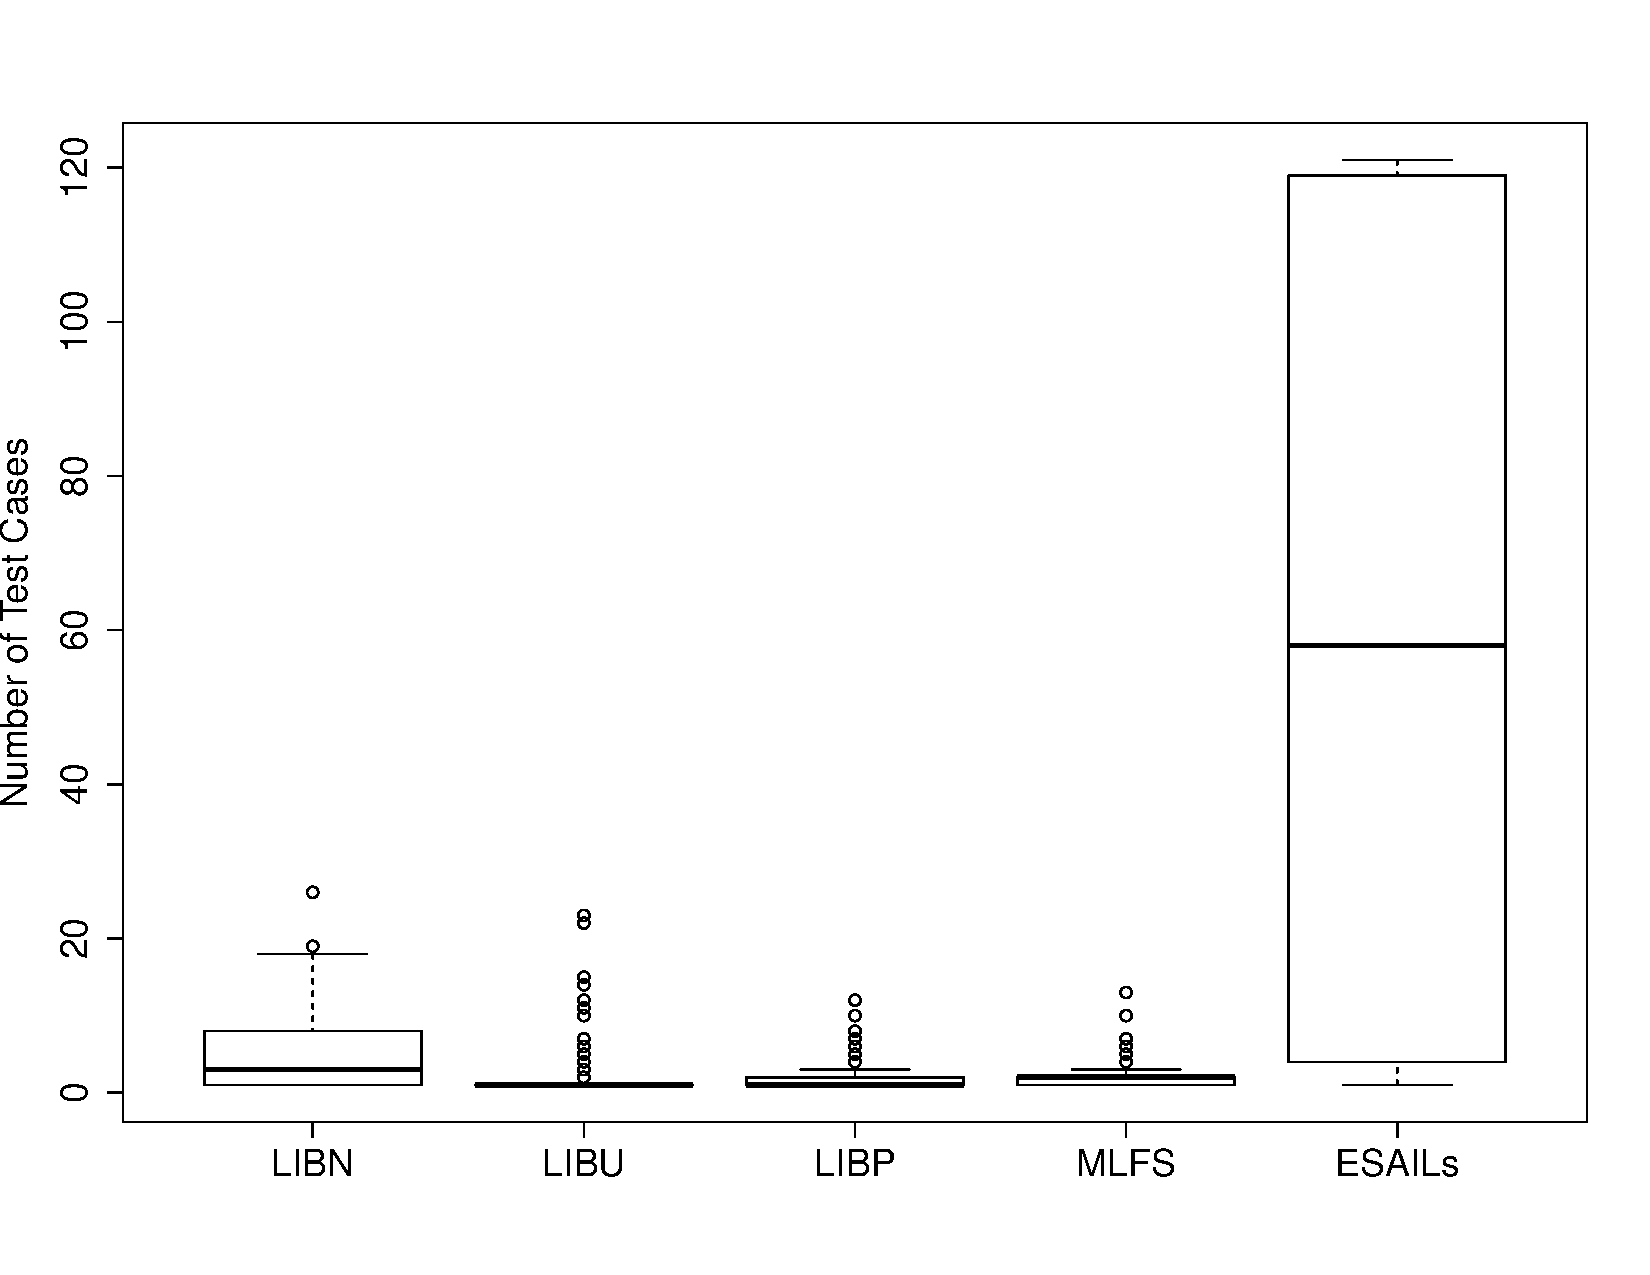
\includegraphics[width=0.8\columnwidth]{images/st_testcases}
\caption{Distribution of test cases exercising each statement.}
\label{fig:tastCaseDist}
\end{center}
\end{figure}

%> min(csp$V1)
%[1] 1
%> min(util$V1)
%[1] 1
%> min(param$V1)
%[1] 1
%> min(mlfs$V1)
%[1] 1
%> min(esail$V1)
%[1] 1
%> max(csp$V1)
%[1] 26
%> max(util$V1)
%[1] 23
%> max(param$V1)
%[1] 12
%> max(mlfs$V1)
%[1] 13
%> max(esail$V1)
%[1] 121
%> mean(csp$V1)
%[1] 4.493617
%> mean(util$V1)
%[1] 1.745416
%> mean(param$V1)
%[1] 2.760691
%> mean(mlfs$V1)
%[1] 2.524808
%> mean(esail$V1)
%[1] 60.96341
%> median(csp$V1)
%[1] 3
%> median(util$V1)
%[1] 1
%> median(param$V1)
%[1] 1
%> median(mlfs$V1)
%[1] 2
%> median(esail$V1)
%[1] 58
%                   [,csp] [,uti] [,para] [,mlf] [,esa]
%[lower whisker,]    1    1    1    1    1
%[lower hinge,]       1    1    1    1    4
%[median,]              3    1    1    2   58
%[upper hinge,]      8    1    2     2   119
%[upper whisker,]   18    1    3    3  121


To address some of our research questions, all the mutants must be executed against the test suite, which is not feasible for the case of \SAIL{}\emph{-CSW} due to its large size and test suite. For this reason, we have identified a subsystem of \SAIL{}\emph{-CSW} (hereafter, \emph{\SAIL{}}$_{S}$) that consists of a set of files, selected by \TWO engineers, that are representative of the different functionalities in \SAIL{}\emph{-CSW}: service/protocol layer functions, critical functions of the satellite implemented in high-level drivers, application layer functions.
Details about $\mathit{\SAIL{}}_{S}$ are reported in Table~\ref{table:caseStudies}.
% \FIXME{note that statement coverage is in line with the whole system.}


Except for \SAIL{}\emph{-CSW}, all subjects
are compiled to generate executables for the development environment OS (Linux); we rely on the Gnu Compiler Collection (GCC)  for Linux X86~\cite{GCC} versions 5.3 and 6.3 for \MLFS{}{} and ONE, respectively. \SAIL{}\emph{-CSW} is compiled with the
LEON/ERC32 RTEMS Cross Compilation System, which includes the GCC C/C++ compiler version 4.4.6 for  RTEMS-4.8 (Sparc architecture)~\cite{RTEMS}.

It is important to note that the technical and test suite characteristics described above are very common in embedded software across many industry domains and cyber-physical systems, thus suggesting our results can be generalizable beyond space software. 

% !TEX root =  ../Main.tex

\begin{table}[tb]
\caption{Descriptions of software components.}
\label{table:caseStudies} 
\scriptsize
\centering
\begin{tabular}{|
@{\hspace{1pt}}p{12mm}
@{\hspace{2pt}}|
@{\hspace{1pt}}>{\raggedleft\arraybackslash}p{8mm}@{\hspace{1pt}}|
@{\hspace{1pt}}>{\raggedleft\arraybackslash}p{18mm}@{\hspace{1pt}}|
@{\hspace{1pt}}>{\raggedleft\arraybackslash}p{20mm}@{\hspace{1pt}}|
@{\hspace{1pt}}>{\raggedleft\arraybackslash}p{24mm}@{\hspace{1pt}}|
p{20mm}|}
\hline
\textbf{Component}&\textbf{LOC}&\textbf{Test suite type}&\textbf{\# Test cases}&\textbf{Statements} \textbf{coverage}\\
\hline
ESAIL& 74155 & System& 384 & 90.38\% \\
ESAIL$_S$& 2235 & System& 384 & 95.36\%\\
LIBGSCSP& 9836 & Integration& 89 & 63.10\%\\
LIBPARAM& 3179 & Integration& 170 & 77.60\%\\
LIBUTIL& 10576 & Unit& 201 & 83.20\%\\
MLFS& 5402 & Unit& 4042 & 100.00\%\\
%MLFS$_V$& 5402 & 4042 & 100.00\%\\
\hline
\end{tabular}

\end{table}

% !TEX root =  ../Main.tex

\begin{table}[tb]
\caption{Generated and compiled mutants per component.}
\label{table:mutants} 
\scriptsize
\begin{tabular}{|
@{\hspace{1pt}}p{12mm}
@{\hspace{2pt}}|
>{\raggedleft\arraybackslash}p{8mm}@{\hspace{1pt}}|
>{\raggedleft\arraybackslash}p{12mm}@{\hspace{1pt}}|
>{\raggedleft\arraybackslash}p{12mm}@{\hspace{1pt}}|
>{\raggedleft\arraybackslash}p{12mm}@{\hspace{1pt}}|
>{\raggedleft\arraybackslash}p{12mm}|}
\hline
\textbf{Component}&\multicolumn{1}{c|}{\textbf{Mutants}}&\multicolumn{1}{c|}{\textbf{Mutants}}&\multicolumn{1}{c|}{\textbf{Mutants}}&\multicolumn{1}{c|}{\textbf{\% of}}&\multicolumn{1}{c|}{\textbf{Mutants}}\\
\textbf{}&\multicolumn{1}{c|}{\textbf{generated}}&\multicolumn{1}{c|}{\textbf{generation}}&\multicolumn{1}{c|}{\textbf{compiled}}&\multicolumn{1}{c|}{\textbf{compiled}}&\multicolumn{1}{c|}{\textbf{compilation}}\\ 
&&\textbf{time} \textbf{(sec)}&&\multicolumn{1}{c|}{\textbf{mutants}}&\multicolumn{1}{c|}{\textbf{time} \textbf{(sec)}}\\ 
\hline
ESAIL& 142763 & 182 &121848& 85.35\% & 151234\\
ESAIL$_S$& & & & &\\
LIBGSCSP& 8666 & 12 &7878&90.91\% & 11425\\
LIBPARAM& 7252 & 7 &6440&88.80\% & 9392\\
LIBUTIL& 22295 & 28 &20268&90.91\% & 30624\\
MLFS& 31526 & 20 &28069&89.03\% &3157\\
%MLFS$_V$& 31526 &T &28069&89.03\% &X\\
\hline
\textbf{Total*}& 212502 & 249 & 184503 &86.82\% &205832\\ 
\hline
\end{tabular}

* We ignore ESAIL$_S$ from the total counting because it is a subset of ESAIL.
\end{table}



\subsection{Setup}
\label{experimnt:setup}

%We should describe the operators used. Potentially could be the superset that is the union of all the operators used in the papers indicated above.
To perform the empirical evaluation, 
%we have implemented the \APPR pipeline in a toolset that is available under the ESA Software Community Licence Permissive~\cite{ESAlicence} at the following URL \textbf{https://faqas.uni.lu/}.
%%\footnote{Prior to acceptance, files are shared at {https://dropit.uni.lu/invitations?share=18629a285f6aceacd026}}.
%For the implementation of mutation operators, we extended the SRCiror toolset~\cite{hariri2018srciror}.
%In our analysis, 
we consider all the operators reported in Table 1.2 from D2.
Related studies~\cite{zhang2010operator,zhang2013operator} are performed by relying on mutation adequate test suites (i.e., test suites that kill all non-equivalent mutants). 
Such test suites are typically automatically generated using static analysis~\cite{papadakis2012mutation}.
%Since our subject artifacts, as it is common in cyber-physical domains, either require dedicated simulators or include network components, we cannot rely on static analysis to generate mutation adequate test suites. 
%We thus rely on the original test suites provided with the subjects. 
\JMR{3.13}{Since we cannot leverage static analysis to generate mutation adequate test suites (see Section~1.2.1.5 from D2), 
we rely on the original test suites provided with the subjects.}
As a result, to perform our study, we mutate only the statements that are covered by the considered test suites.

\CHANGED{For every subject, we generated mutants by executing the \APPR toolset on Linux OS running on a MacBook Pro with 2,3 GHz 8-Core Intel Core i9. 
Table~\ref{table:mutants} reports, for every subject, the total number of mutants that were generated, their generation time, the number of mutants successfully compiled, the proportion of compiled mutants with respect to the overall number of mutants generated, and the time required to compile mutants using one compiler optimization level only (i.e., the one originally selected by engineers for each subject).
%the default compiler optimization options of the subject.
The generation of mutants is fast, it takes at most {182} seconds on the largest subject (\SAIL{}\emph{-CSW}). On average, across subjects, it takes {11} milliseconds to generate a single mutant. 
The proportion of successfully compiled mutants is large (i.e., 86.82\% overall), though it varies from 85.35\% for \SAIL{}\emph{-CSW} to 90.91\% for \GCSP{} and \UTIL{}.
This proportion is in line with the ones reported in related work, though there is variation. For example, industrial systems 
%that likely contain complex instructions, 
have shown lower success rates (e.g., 81.13\% for safety-critical software components~\cite{Baker2013}) than open source, batch utilities (e.g., 96.30\% for Coreutils~\cite{hariri2016evaluating}).} \REVNOV{PTCR-17}{In the case of compiler warnings, we simply follow the policy configured for the case study. More precisely., in the case of ESAIl and MLFS all the warnings from the compiler lead to a compilation failure. In the case of GSL the compilation process proceeds.}
 
{As shown in Table~\ref{table:mutants}, the time required to compile all the mutants ranges from 3,157 to 151,234 seconds, for an average of 0.96 seconds required to compile a single mutant, across subjects. Because of our selective compilation strategy (see Section~1.2.7 from D2), the time required by our pipeline to compile a single mutant is significantly lower than the one required by state-of-the-art approaches, which is around 4.6 seconds per mutant, even when software components have a lower number of LOC %(i.e., 22,827 LOC)  
than our subjects~\cite{kintis2017detecting}.}

% {The last three columns of Table~\ref{table:mutants} present the number and percentage of mutants successfully compiled, along with the time required to compile all the mutants using the proposed incremental compilation process (Step 3 of \APPR). 
%In total, 86.82\% of the mutants generated among the four case study systems are successfully compiled. 
 



%According to previous research on mutant operator selection, we consider the superset, that is, the union of all the operators defined in the work by Offutt et al.~\cite{offutt1996experimental}, Andrews et al.~\cite{andrews2005mutation} and Kintis et al.~\cite{kintis2017detecting}. The superset consist of the AOR, LCR, ICR, ROR, SDL, UOI, and ABS.
%
%To asses our research questions with the different set of operators considered in the literature, we consider four interleaving subsets of the : the sufficient set (i.e., AOR, LCR, ICR, ROR, SDL, UOI, and ABS),
%the deletion set (i.e., SDL, AOD, LOD, ROD, BOD, and SOD), the extended sufficient set (i.e., all the operators in Table~\ref{table:operators}), and the statement deletion set (i.e., the SDL operator only).  



{To collect the data required to address research questions RQ2 to RQ8, for every subject and unique mutant generated by Step 3, we have executed all the test cases covering the mutated statement. Table~\ref{table:magnitude} provides, for every subject, the overall number of executed test cases and the total execution time required for our experiments. In total, the entire experiment took 1,912,662 minutes (31,878 hours or more than 1300 days). Test  execution time depends on the number of mutants, the number of executed test cases, and the test suite level (e.g., system test suites exercise more complex scenarios than unit or integration test suites).}  
%In our experiments, the execution times of the components tested with unit test suites \FIXME{have the same order of magnitude; indeed, they take between X and Y seconds to execute.}
%In the case of ESAIL, instead, \FIXME{....}}

\CHANGED{To be able to execute test cases for 31,878 hours, we performed our experiments using the HPC cluster of the University of Luxembourg~\cite{HPC}.
The HPC cluster consists of Intel Xeon E5-2680 v4 (2.4 GHz) nodes. To perform our experiments, we tested 100 mutants in parallel, each one on a dedicated node.}

% !TEX root =  ../Main.tex

\begin{table}[tb]
\caption{Experiments magnitude.}
\label{table:magnitude} 
\scriptsize
\centering
\begin{tabular}{|
@{\hspace{1pt}}p{12mm}
@{\hspace{2pt}}|
@{\hspace{1pt}}>{\raggedleft\arraybackslash}p{30mm}@{\hspace{1pt}}|
@{\hspace{1pt}}>{\raggedleft\arraybackslash}p{35mm}@{\hspace{1pt}}|
p{20mm}|}
\hline
\textbf{Case Study}&\textbf{Total test cases executed}&\textbf{Total execution time (minutes)}\\
\hline
%Fabrizio: after removing tests that do not cover the mutants, we should have lower numbers
ESAIL$_S$&  302\,158 & 1\,624\,336\\
LIBGSCSP&  771\,274 & 33\,756\\
LIBPARAM&  1\,094\,800 & 7\,205\\
LIBUTIL&  4\,481\,295 & 57\,732\\
MLFS&  170\,303\,452 & 189\,633\\
%MLFS$_V$& 5402 & 4042 & 100.00\%\\
\hline
\textbf{Total}&  176\,952\,979 & 1\,912\,662\\
\hline
\end{tabular}

\end{table}

In the following sections, we 
%analyze differences in results 
\JMR{3.11}{discuss statistical significance}
using a non-parametric Mann Whitney U-test (with $\alpha$ = 0.05)~\cite{Arcuri:practicalGuide:ICSE:2015}.  We discuss effect size based on Vargha and Delaney’s $A_{12}$ statistics, a non-parametric effect size measure~\cite{VDA,Arcuri:practicalGuide:ICSE:2015}. Based on $A_{12}$, effect size is considered small when $0.56 \le A_{12} < 0.64$, medium when $0.64 \le A_{12} < 0.71$, large when $A_{12} \ge 0.71$. Otherwise the compared samples are considered equivalent, that is to be drawn from the same population~\cite{VDA}.


% % !TEX root =  ../Main.tex

\newcommand{\op}{\mathit{op}}
\newcommand{\ArithmeticSet}{ \texttt{+}, \texttt{-}, \texttt{*}, \texttt{/}, \texttt{\%} }
\newcommand{\LogicalSet}{ \texttt{&&}, \texttt{||} }
\newcommand{\RelationalSet}{ \texttt{>}, \texttt{>=}, \texttt{<}, \texttt{<=}, \texttt{==}, \texttt{!=} }
\newcommand{\BitWiseSet}{ \texttt{\&}, \texttt{|}, \land }
\newcommand{\ShiftSet}{ \texttt{>>}, \texttt{<<} }


\begin{table}[h]
\caption{Implemented set of mutation operators.}
\label{table:operators} 
\centering
\scriptsize
\begin{tabular}{|@{}p{4mm}@{}|@{}p{2cm}@{\hspace{1pt}}|@{}p{11.1cm}@{}|}
\hline
&\textbf{Operator} & \textbf{Description$^{*}$} \\
\hline
\multirow{7}{*}{\rotatebox{90}{\emph{Sufficient Set}}}&ABS               & $\{(v, -v)\}$	\\
\cline{2-3}
&AOR               & $\{(\op_1, op_2) \,|\, \op_1, \op_2 \in \{ \ArithmeticSet \} \land \op_1 \neq \op_2 \} $       \\
&    			  & $\{(\op_1, \op_2) \,|\, \op_1, \op_2 \in \{\texttt{+=}, \texttt{-=}, \texttt{*=}, \texttt{/=}, \texttt{\%} \texttt{=}\} \land \op_1 \neq \op_2 \} $       \\
\cline{2-3}
&ICR               & $\{i, x) \,|\, x \in \{1, -1, 0, i + 1, i - 1, -i\}\}$           \\
\cline{2-3}
&LCR               & $\{(\op_1, \op_2) \,|\, \op_1, \op_2 \in \{ \texttt{\&\&}, || \} \land \op_1 \neq \op_2 \}$            \\
&				  & $\{(\op_1, \op_2) \,|\, \op_1, \op_2 \in \{ \texttt{\&=}, \texttt{|=}, \texttt{\&=}\} \land \op_1 \neq \op_2 \}$            \\
&				  & $\{(\op_1, \op_2) \,|\, \op_1, \op_2 \in \{ \texttt{\&}, \texttt{|}, \texttt{\&\&}\} \land \op_1 \neq \op_2 \}$            \\
\cline{2-3}
&ROR               & $\{(\op_1, \op_2) \,|\, \op_1, \op_2 \in \{ \RelationalSet \}\}$            \\
&				  & $\{ (e, !(e)) \,|\, e \in \{\texttt{if(e)}, \texttt{while(e)}\} \}$ \\
\cline{2-3}
&SDL               & $\{(s, \texttt{remove}(s))\}$            \\
\cline{2-3}
&UOI               & $\{ (v, \texttt{--}v), (v, v\texttt{--}), (v, \texttt{++}v), (v, v\texttt{++}) \}$            \\   
\hline
\hline
\multirow{5}{*}{\rotatebox{90}{\emph{OODL}}}&AOD               & $\{((t_1\,op\,t_2), t_1), ((t_1\,op\,t_2), t_2) \,|\, op \in \{ \ArithmeticSet \} $       \\ 
\cline{2-3}
&LOD               & $\{((t_1\,op\,t_2), t_1), ((t_1\,op\,t_2), t_2) \,|\, op \in \{  \} \}$       \\ 
\cline{2-3}
&ROD               & $\{((t_1\,op\,t_2), t_1), ((t_1\,op\,t_2), t_2) \,|\, op \in \{ \RelationalSet \} \}$       \\ 
\cline{2-3}
&BOD               & $\{((t_1\,op\,t_2), t_1), ((t_1\,op\,t_2), t_2) \,|\, op \in \{ \BitWiseSet \} \}$       \\ 
\cline{2-3}
&SOD               & $\{((t_1\,op\,t_2), t_1), ((t_1\,op\,t_2), t_2) \,|\, op \in \{ \ShiftSet \} \}$       \\ 
%\hline
%COR               & $\{(\op_1, \op_2) \,|\, \op_1, \op_2 \in \{ \texttt{\&\&}, \texttt{||}, \land \} \land \op_1 \neq \op_2 \}$            \\
\hline
\hline
\multirow{3}{*}{\rotatebox{90}{\emph{Other}}}&LVR			& $\{(l_1, l_2) \,|\, (l_1, l_2) \in \{(0,-1), (l_1,-l_1), (l_1, 0), (\mathit{true}, \mathit{false}), (\mathit{false}, \mathit{true})\}\}$\\
&&\\
&&\\
\hline
\end{tabular}

$^{*}$Each pair in parenthesis shows how a program element is modified by the mutation operator. Th eleft element of the pair is replaced with the right element. We follow standard syntax~\cite{kintis2018effective}. Program elements are literals ($l$), integer literals ($i$), boolean expressions ($e$), operators ($\op$), statements ($s$), variables ($v$), and terms ( $t_i$, which might be either variables or literals).
\end{table}

%To generate the mutants, we have extended the SRCIRor mutation testing tool~\cite{hariri2018srciror}. since the original version only implemented the set of operators AOR, LCR, ICR and ROR.

%For each subject of the study we generated mutants by applying the sufficient set of operators. We call this set of mutants complete mutants set.

%We executed the test suites of the case study systems against the complete mutants set. Test execution results let us compute the mutation score of the case study. For each case study, we kept track of the mutants killed by each test case.




%
%To address our research questions considering test suites with different mutation scores for the complete mutants set, for each case study, we derived subsets of the original test suites with different mutation scores. The test suites were randomly derived by randomly selecting test cases till a specific mutation score is reached. We consider test suites with the following mutation scores...

\subsection{RQ1}

% !TEX root =  ../Main.tex
\begin{table*}[htb]
\caption{RQ1. Proportion (\%) of Trivially-Equivalent and Trivially-Redundant Mutants Detected by Compiler Optimizations.}
\label{table:results:compilerOptimizations} 
\tiny
\centering
%\begin{tabular}{|
%p{11mm}|p{6mm}|p{10mm}|
%@{\hspace{2mm}}p{5mm}|p{5mm}|p{5mm}|p{5mm}|p{5mm}|p{5mm}|
%p{6mm}|p{6mm}|p{6mm}|p{6mm}|p{6mm}|p{6mm}|
%}
%\hline
%\textbf{Case} & \textbf{All} & \textbf{Compiled} & \multicolumn{6}{c|}{Equivalent} & \multicolumn{6}{c|}{Redundant} \\
%\textbf{Study}& & 
%&\textbf{O0}&\textbf{O1} & \textbf{O2} & \textbf{O3} & \textbf{Os} & \textbf{Of} 
%&\textbf{O0}&\textbf{O1} & \textbf{O2} & \textbf{O3} & \textbf{Os} & \textbf{Of}
%\\
%\hline
%ESAIL & 142763 & 121848 & 3029 & 8440 & 8520 & 8472 & 8634 & - & 14032 & 21011 & 21768 & 21613 & 21943 & - \\
% &  &  & 2.49  & 6.93  & 6.70  & 6.95  & 7.09  & - & 11.52  & 17.25  & 17.86  & 17.74  & 18.01  & - \\
%LIBUTIL & 22295 & 20268 & 394 & 1277 & 1233 & 1255 & 1247 & 1255 & 2093 & 3092 & 3320 & 3369 & 3383 & 3369 \\
% &  &  & 1.94  & 6.30  & 6.08  & 6.19  & 6.15  & 6.19  & 10.33  & 15.26  & 16.38  & 16.62  & 16.69  & 16.62  \\
%LIBPARAM & 7252 & 6440 & 151 & 428 & 423 & 425 & 436 & 425 & 909 & 1310 & 1346 & 1346 & 1348 & 1346 \\
% &  &  & 2.34  & 6.65  & 6.57  & 6.60  & 6.77  & 6.60 & 14.11  & 20.34  & 20.90  & 20.90  & 20.93  & 20.90  \\
%LIBGSCSP & 8666 & 7878 & 176 & 683 & 511 & 519 & 315 & 336 & 997 & 1756 & 1332 & 1528 & 1690 & 1672 \\
% &  &  & 2.23  & 8.67  & 6.49  & 6.59  & 4.00  & 4.27  & 12.66  & 22.29  & 16.91  & 19.40  & 21.45  & 21.22  \\
%MLFS & 31526 & 28069 & 115 & 230 & 281 & 282 & 307 & 293 & 2386 & 3244 & 3620 & 3628 & 3732 & 3895 \\
% &  &  & 0.41  & 0.82  & 1.00  & 1.00  & 1.09  & 1.04  & 8.50  & 11.55  & 12.90  & 12.93  & 13.30  & 13.88  \\
%\hline
%\textbf{Total}  & 212502 & 184503 & 3773 & 10559 & 10963 & 10557 & 11211 & 2096 & 20479 & 30414 & 31568 & 31800 & 31867 & 10458\\
%&  &  & 2.04  & 5.72  & 5.94  & 5.72  & 6.08  & 1.14  & 11.10  & 16.48  & 17.11  & 17.24  & 17.27  & 5.67  \\
%\hline
%
%\end{tabular}

\begin{tabular}{|
p{11mm}|
@{\hspace{1pt}} >{\raggedleft\arraybackslash}p{9mm}@{\hspace{1pt}}|
@{\hspace{1pt}}>{\raggedleft\arraybackslash}p{10mm}@{\hspace{1pt}}|
@{\hspace{1pt}}>{\raggedleft\arraybackslash}p{8mm}@{\hspace{1pt}}|
>{\raggedleft\arraybackslash}p{5mm}@{\hspace{1pt}}|
>{\raggedleft\arraybackslash}p{8mm}@{\hspace{1pt}}|
 >{\raggedleft\arraybackslash}p{5mm}@{\hspace{1pt}}|
 >{\raggedleft\arraybackslash}p{5mm}@{\hspace{1pt}}|
 >{\raggedleft\arraybackslash}p{5mm}@{\hspace{1pt}}|
 >{\raggedleft\arraybackslash}p{5mm}@{\hspace{1pt}}|
>{\raggedleft\arraybackslash}p{7mm}@{\hspace{1pt}}|
@{\hspace{1pt}} >{\raggedleft\arraybackslash}p{10mm}@{\hspace{1pt}}|
@{\hspace{1pt}} >{\raggedleft\arraybackslash}p{8mm}@{\hspace{1pt}}|
 >{\raggedleft\arraybackslash}p{8mm}@{\hspace{1pt}}|
 >{\raggedleft\arraybackslash}p{6mm}@{\hspace{1pt}}|
 >{\raggedleft\arraybackslash}p{6mm}@{\hspace{1pt}}|
 >{\raggedleft\arraybackslash}p{6mm}@{\hspace{1pt}}|
 >{\raggedleft\arraybackslash}p{6mm}@{\hspace{1pt}}|
 >{\raggedleft\arraybackslash}p{6mm}@{\hspace{1pt}}|
}







\hline
\textbf{Case} & \multicolumn{9}{c|}{\textbf{Equivalent}} & \multicolumn{9}{c|}{\textbf{Redundant}} \\
\textbf{Study}
&\textbf{All}&\textbf{Overall}\textbf{\%}&\textbf{-O0-3}&\textbf{-O0}&\textbf{-O1} & \textbf{-O2} & \textbf{-O3} & \textbf{-Os} & \textbf{-Of} 
&\textbf{All}&\textbf{Overall}\textbf{\%}&\textbf{-O0-3}&\textbf{-O0}&\textbf{-O1} & \textbf{-O2} & \textbf{-O3} & \textbf{-Os} & \textbf{-Of}
\\
\hline
ESAIL &8861&7.27 &7.13&34.18 &95.25 &96.15 &95.61 &97.44 &-&35133&28.83&27.74&39.94 &59.80 &61.96 &61.52 &62.46 &-\\
LIBUTIL &1366&6,74 &6.65&28.84 &93.48 &90.26 &91.87 &91.29 &91.87 &4392&21.67&21.26&47.65 &70.40 &75.59 &76.71 &77.03 &76.71 \\
LIBPARAM &450& 6.99 &6.89&33.56 &95.11 &94.00 &94.44 &96.89 &94.44 &2076&32.24&31.44&43.79 &63.10 &64.84 &64.84 &64.93 &64.84 \\
LIBGSCSP &701&8.90 &8.90&25.11 &97.43 &72.90 &74.04 &44.94 &47.93 &2655&33.70&27.63&37.55 &66.14 &50.17 &57.55 &63.65 &62.98 \\
MLFS &361 &1.29 &1.04&31.86 &63.71 &77.84 &78.12 &85.04 &81.16 &6356&22.64&20.13&37.54 &51.04 &56.95 &57.08 &58.72 &61.28 \\
\hline
\textbf{Total}  &11739&6.36 &6.22&32.14 &89.95 &93.39 &89.93 &95.50 &17.86 &50612&27.43&25.99&40.46 &60.09 &62.37 &62.83 &62.96 &20.66 \\
\hline

\end{tabular}


\end{table*}

\begin{table*}[htb]
\caption{RQ1.  Proportion (\%) of Univocal-Trivially-Equivalent and Univocal-Trivially-Redundant Mutants Detected by Compiler Optimizations.}
\label{table:results:compilerOptimizationsUnivocal} 
\tiny
%\centering
%\begin{tabular}{|
%p{11mm}|p{6mm}|p{10mm}|
%@{\hspace{2mm}}p{6mm}|p{6mm}|p{6mm}|p{6mm}|p{6mm}|p{6mm}|
%p{6mm}|p{6mm}|p{6mm}|p{6mm}|p{6mm}|p{6mm}|
%}
%\hline
%\textbf{Case} & \textbf{All} & \textbf{Compiled} & \multicolumn{6}{c|}{Univocal-Equivalent} & \multicolumn{6}{c|}{Univocal-Redundant} \\
%\textbf{Study}& & 
%&\textbf{O0}&\textbf{O1} & \textbf{O2} & \textbf{O3} & \textbf{Os} & \textbf{Of} 
%&\textbf{O0}&\textbf{O1} & \textbf{O2} & \textbf{O3} & \textbf{Os} & \textbf{Of}
%\\
%\hline
%
%ESAIL & 142763 & 121848 & 0 & 11 & 2 & 47 & 177 & - & 516 & 999 & 1033 & 1175 & 1334 & - \\
%  & & & 0.000  & 0.009  & 0.001  & 0.039  & 0.145  & - & 0.423  & 0.819  & 0.850  & 0.964  & 1.094  & - \\
%LIBUTIL & 22295 & 20268 & 1 & 74 & 2 & 0 & 19 & 0 & 818 & 48 & 4 & 0 & 79 & 4\\
% & & & 0.005  & 0.365  & 0.010  & 0.000  & 0.094  & 0.000  & 4.036  & 0.237  & 0.019  & 0.000  & 0.389  & 0.019  \\
%LIBPARAM & 7252 & 6440 & 0 & 5 & 0 & 0 & 6 & 0 & 20 & 55 & 54 & 0 & 51 & 0\\
% & & & 0.000  & 0.078  & 0.000  & 0.000  & 0.093  & 0.000   & 0.311  & 0.854  & 0.839  & 0.000  & 0.791  & 0.000  \\
%LIBGSCSP & 8666 & 7878 & 0 & 0 & 7 & 0 & 23 & 0 & 1 & 58 & 89 & 0 & 98 & 0\\
% & & & 0.000  & 0.000  & 0.089  & 0.000  & 0.292  & 0.000  & 0.013  & 0.736  & 1.130  & 0.000  & 1.244  & 0.000  \\
%MLFS & 31526 & 28069 & 0 & 6 & 0 & 0 & 39 & 20 & 6 & 60 & 340 & 2 & 443 & 256\\
% & & & 0.000  & 0.021  & 0.000  & 0.000  & 0.139  & 0.071  & 0.021  & 0.214  & 1.211  & 0.007  & 1.578  & 0.912  \\
%\hline
%\textbf{Total}  & 212502 & 184503 & 1 & 96 & 11 & 47 & 264 & 20 & 1046 & 2113 & 529 & 277 & 3114 & 318 \\
% & & & 0.001  & 0.052  & 0.001  & 0.025  & 0.143  & 0.011  & 0.567  & 1.145  & 0.287  & 0.150  & 1.689  & 0.172  \\
%\hline
%
%\end{tabular}

\begin{tabular}{|
p{11mm}|
@{\hspace{1pt}} >{\raggedleft\arraybackslash}p{9mm}@{\hspace{1pt}}|
@{\hspace{1pt}}>{\raggedleft\arraybackslash}p{19mm}@{\hspace{1pt}}|
>{\raggedleft\arraybackslash}p{5mm}@{\hspace{1pt}}|
>{\raggedleft\arraybackslash}p{8mm}@{\hspace{1pt}}|
 >{\raggedleft\arraybackslash}p{5mm}@{\hspace{1pt}}|
 >{\raggedleft\arraybackslash}p{5mm}@{\hspace{1pt}}|
 >{\raggedleft\arraybackslash}p{5mm}@{\hspace{1pt}}|
 >{\raggedleft\arraybackslash}p{5mm}@{\hspace{1pt}}|
>{\raggedleft\arraybackslash}p{7mm}@{\hspace{1pt}}|
@{\hspace{1pt}} >{\raggedleft\arraybackslash}p{19mm}@{\hspace{1pt}}|
 >{\raggedleft\arraybackslash}p{8mm}@{\hspace{1pt}}|
 >{\raggedleft\arraybackslash}p{6mm}@{\hspace{1pt}}|
 >{\raggedleft\arraybackslash}p{6mm}@{\hspace{1pt}}|
 >{\raggedleft\arraybackslash}p{6mm}@{\hspace{1pt}}|
 >{\raggedleft\arraybackslash}p{6mm}@{\hspace{1pt}}|
 >{\raggedleft\arraybackslash}p{6mm}@{\hspace{1pt}}|
}







\hline
\textbf{Case} & \multicolumn{8}{c|}{\textbf{Univocal-Equivalent}} & \multicolumn{8}{c|}{\textbf{Univocal-Redundant}} \\
\textbf{Study}
&\textbf{All}&\textbf{\%} \textbf{of} \textbf{Equivalent}&\textbf{-O0}&\textbf{-O1} & \textbf{-O2} & \textbf{-O3} & \textbf{-Os} & \textbf{-Of} 
&\textbf{All}&\textbf{\%} \textbf{of} \textbf{Redundant}&\textbf{-O0}&\textbf{-O1} & \textbf{-O2} & \textbf{-O3} & \textbf{-Os} & \textbf{-Of}
\\
\hline
ESAIL &237& 2.67&0.00 &4.64 &0.84 &19.83 &\textbf{74.68} &0.00 &5057&14.39&10.20 &19.75 &20.43 &23.24 &\textbf{26.38} &0.00  \\
LIBUTIL &96& 7.03&1.04 &77.08 &2.08 &0.00 &\textbf{19.79} &0.00 &953& 21.70&\textbf{85.83} &5.04 &0.42 &0.00 &8.29 &0.42  \\
LIBPARAM &11 & 2.44&0.00 &45.45 &0.00 &0.00 &\textbf{54.55} &0.00 &180& 8.67&11.11 &\textbf{30.56} &30.00 &0.00 &28.33 &0.00  \\
LIBGSCSP &112 & 15.98&25.11 &\textbf{97.43} &72.90 &74.04 &44.94 &47.93 &429& 16.16&37.55 &\textbf{66.14} &50.17 &57.55 &63.65 &62.98  \\
MLFS &65& 18.01&0.00 &9.23 &0.00 &0.00 &60.00 &\textbf{30.77} &1107& 17.42&0.54 &5.42 &30.71 &0.18 &\textbf{40.02} &23.13 \\
\hline
\textbf{Total}  &521& 4.44&0.19 &18.43 &2.11 &9.02 &\textbf{50.67} &3.84 &7726& 15.27&13.54 &27.35 &6.85 &3.59 &\textbf{40.31} &4.12 \\
\hline

\end{tabular}


\end{table*}


% \begin{table*}[htb]
% \caption{RQ1. Equivalent and Redundant Mutants Detected by Compiler Optimizations.}
% \label{table:results:compilerOptimizations} 
% \tiny
% \begin{tabular}{|
% p{7mm}|p{5mm}|p{7mm}|
% @{\hspace{1mm}}p{4mm}|p{2mm}|p{2mm}|p{2mm}|p{2mm}|p{2mm}|p{2mm}|
% p{2mm}|p{2mm}|p{2mm}|p{2mm}|p{2mm}|p{2mm}|
% p{2mm}|p{2mm}|p{2mm}|p{2mm}|p{2mm}|p{2mm}|
% p{2mm}|p{2mm}|p{2mm}|p{2mm}|p{2mm}|p{2mm}|
% }
% \hline
% \textbf{Case} & \textbf{All} & \textbf{Compiled} & \multicolumn{6}{c|}{Equivalent} & \multicolumn{6}{c|}{Redundant} 
% & \multicolumn{6}{c|}{Univocal-Equivalent}  & \multicolumn{6}{c|}{Univocal-Redundant} \\
% \textbf{Study}&&
% &\textbf{O0}&\textbf{O1} & \textbf{O2} & \textbf{O3} & \textbf{Os} & \textbf{Of} 
% &\textbf{O0}&\textbf{O1} & \textbf{O2} & \textbf{O3} & \textbf{Os} & \textbf{Of}
% &\textbf{O0}&\textbf{O1} & \textbf{O2} & \textbf{O3} & \textbf{Os} & \textbf{Of} 
% &\textbf{O0}&\textbf{O1} & \textbf{O2} & \textbf{O3} & \textbf{Os} & \textbf{Of}
% \\
% ESAIL & 142763 & 121848 & 3029 & 8440 & 8520 & 8472 & 8634 &  & 14032 & 21013 & 21768 & 21613 & 21944 & & 0 & 11 & 2 & 47 & 177 & & 1032 & 1923 & 90 & 240 & 2463 & \\
%  &  &  & 2.49  & 6.93  & 6.70  & 6.95  & 7.09  &  & 11.52  & 17.25  & 17.86  & 17.74  & 18.01  & & 0.00  & 9e-03  & 1.6e-03  & 0.04  & 0.15  &  & 0.85  & 1.58  & 0.07   & 0.2  & 2.02  & \\
% LIBUTIL & 22295 & 20268 & 394 & 1277 & 1233 & 1255 & 1247 & 1255 & 2093 & 3092 & 3319 & 3364 & 3381 & 3368 & 1 & 74 & 2 & 0 & 19 & 0 & 7 & 56 & 7 & 35 & 87 & 62\\
% LIBPARAM & 7252 & 6440 & 151 & 428 & 423 & 425 & 436 & 425 & 909 & 1309 & 1346 & 1346 & 1347 & 1346 & 0 & 5 & 0 & 0 & 6 & 0 & 0 & 16 & 3 & 0 & 23 & 0\\
% LIBGSCSP & 8666 & 7878 & 84 & 184 & 506 & 123 & 587 & 123 & 1059 & 1756 & 1515 & 1849 & 1463 & 1849 & 0 & 0 & 7 & 0 & 23 & 0 & 1 & 58 & 89 & 0 & 98 & 0\\
% MLFS & 31526 & 28069 & 115 & 230 & 281 & 282 & 307 & 293 & 2386 & 3244 & 3620 & 3628 & 3732 & 3895 & 0 & 6 & 0 & 0 & 39 & 20 & 6 & 60 & 340 & 2 & 443 & 256\\
% \hline
% \textbf{Total}  & 212502 & 184503 & 3773 & 10559 & 10963 & 10557 & 11211 & 2096 & 20479 & 30414 & 31568 & 31800 & 31867 & 10458 & 1 & 96 & 11 & 47 & 264 & 20 & 1046 & 2113 & 529 & 277 & 3114 & 318 \\

% %\hline
% %ES\\
% %\hline
% \end{tabular}

% \end{table*}

\begin{table*}[htb]
\caption{RQ1.  Proportion (\%) of Trivially Equivalent/Redundant Mutants Detected per Mutation Operator.}
\label{table:results:compilerOptimizationsProportionOperators} 
\scriptsize
\begin{tabular}{|
p{11mm}|
>{\raggedleft\arraybackslash}p{5mm}@{\hspace{1pt}}|
@{\hspace{1pt}}>{\raggedleft\arraybackslash}p{5mm}@{\hspace{1pt}}|
@{\hspace{1pt}} >{\raggedleft\arraybackslash}p{5mm}@{\hspace{1pt}}|
@{\hspace{1pt}} >{\raggedleft\arraybackslash}p{5mm}@{\hspace{1pt}}|
@{\hspace{1pt}} >{\raggedleft\arraybackslash}p{5mm}@{\hspace{1pt}}|
@{\hspace{1pt}} >{\raggedleft\arraybackslash}p{5mm}@{\hspace{1pt}}|
@{\hspace{1pt}} >{\raggedleft\arraybackslash}p{5mm}@{\hspace{1pt}}|
@{\hspace{1pt}} >{\raggedleft\arraybackslash}p{5mm}@{\hspace{1pt}}|
@{\hspace{1pt}} >{\raggedleft\arraybackslash}p{5mm}@{\hspace{1pt}}|
@{\hspace{1pt}} >{\raggedleft\arraybackslash}p{5mm}@{\hspace{1pt}}|
@{\hspace{1pt}} >{\raggedleft\arraybackslash}p{5mm}@{\hspace{1pt}}|
@{\hspace{1pt}} >{\raggedleft\arraybackslash}p{5mm}@{\hspace{1pt}}|
@{\hspace{1pt}} >{\raggedleft\arraybackslash}p{5mm}@{\hspace{1pt}}|
 >{\raggedleft\arraybackslash}p{5mm}@{\hspace{1pt}}|
@{\hspace{1pt}}>{\raggedleft\arraybackslash}p{5mm}@{\hspace{1pt}}|
@{\hspace{1pt}} >{\raggedleft\arraybackslash}p{5mm}@{\hspace{1pt}}|
@{\hspace{1pt}} >{\raggedleft\arraybackslash}p{5mm}@{\hspace{1pt}}|
@{\hspace{1pt}} >{\raggedleft\arraybackslash}p{5mm}@{\hspace{1pt}}|
@{\hspace{1pt}} >{\raggedleft\arraybackslash}p{5mm}@{\hspace{1pt}}|
@{\hspace{1pt}} >{\raggedleft\arraybackslash}p{5mm}@{\hspace{1pt}}|
@{\hspace{1pt}} >{\raggedleft\arraybackslash}p{5mm}@{\hspace{1pt}}|
@{\hspace{1pt}} >{\raggedleft\arraybackslash}p{5mm}@{\hspace{1pt}}|
@{\hspace{1pt}} >{\raggedleft\arraybackslash}p{5mm}@{\hspace{1pt}}|
@{\hspace{1pt}} >{\raggedleft\arraybackslash}p{5mm}@{\hspace{1pt}}|
@{\hspace{1pt}} >{\raggedleft\arraybackslash}p{5mm}@{\hspace{1pt}}|
@{\hspace{1pt}} >{\raggedleft\arraybackslash}p{5mm}@{\hspace{1pt}}|
}

\hline
\textbf{Case}& \multicolumn{13}{c|}{\textbf{Trivially Equivalent}} &\multicolumn{13}{c|}{\textbf{Trivially Redundant}}\\
\textbf{Study}&
\textbf{ABS}&	\textbf{AOR}&	\textbf{ICR}&	\textbf{LCR}&	\textbf{ROR}&	\textbf{SDL}&	\textbf{UOI}&	\textbf{AOD}&	\textbf{LOD}&	\textbf{ROD}&	\textbf{BOD}&	\textbf{SOD}&	\textbf{LVR}&
\textbf{ABS}&	\textbf{AOR}&	\textbf{ICR}&	\textbf{LCR}&	\textbf{ROR}&	\textbf{SDL}&	\textbf{UOI}&	\textbf{AOD}&	\textbf{LOD}&	\textbf{ROD}&	\textbf{BOD}&	\textbf{SOD}&	\textbf{LVR}\\
\hline
ESAIL&3.65&1.85&6.74&2.09&18.00&1.60&52.34&1.53&0.05&7.64&3.42&0.51&0.59&1.52&6.20&18.79&1.05&23.89&8.04&20.23&4.83&1.06&8.86&2.20&1.96&1.39\\
LIBUTIL&6.66&0.07&3.95&1.24&15.96&7.91&58.86&0.00&0.37&3.81&0.95&0.00&0.22&0.34&7.38&15.64&0.87&30.35&12.61&13.52&1.66&2.66&12.77&0.89&0.52&0.77\\
LIBPARAM&8.89&0.00&0.00&0.22&25.56&6.22&55.33&0.00&0.00&3.56&0.22&0.00&0.00&0.96&3.47&7.95&1.01&36.71&13.58&12.52&1.49&2.46&18.45&0.92&0.00&0.48\\
LIBGSCSP&8.84&0.00&2.28&1.14&17.40&3.14&56.35&0.00&0.14&9.84&0.86&0.00&0.00&2.11&2.37&10.77&1.24&31.45&9.04&23.92&1.69&1.36&13.48&1.58&0.79&0.19\\
MLFS&6.37&0.55&11.63&0.28&27.98&2.77&39.61&0.00&0.00&9.42&1.39&0.00&0.00&5.03&10.12&25.36&0.87&23.77&4.14&6.73&8.51&0.88&9.44&2.33&1.90&0.91\\
\hline
\textbf{Total}&4.59&1.42&6.04&1.81&18.32&2.64&\textbf{53.06}&1.16&0.09&7.22&2.79&0.38&0.47&1.87&6.48&18.47&1.02&25.36&8.23&\textbf{17.83}&4.72&1.25&9.91&2.02&1.68&1.17\\
\hline
\end{tabular}


\end{table*}
% !TEX root =  ../Main.tex

\begin{table}[h]
\caption{RQ1. Compilation Time Required by Compiler Optimization Techniques.}
\label{table:results:compilerOptimizationsTime} 
\tiny
\centering
\begin{tabular}{|
@{\hspace{1pt}}p{11mm}|
@{\hspace{1pt}}>{\raggedleft\arraybackslash}p{7mm}@{\hspace{1pt}}|
>{\raggedleft\arraybackslash}p{7mm}@{\hspace{1pt}}|
>{\raggedleft\arraybackslash}p{7mm}@{\hspace{1pt}}|
>{\raggedleft\arraybackslash}p{7mm}@{\hspace{1pt}}|
>{\raggedleft\arraybackslash}p{7mm}@{\hspace{1pt}}|
>{\raggedleft\arraybackslash}p{7mm}@{\hspace{1pt}}|
 >{\raggedleft\arraybackslash}p{16mm}@{\hspace{1pt}}|
}
\hline
\textbf{Case} & 
\multicolumn{7}{c|}{\textbf{Time required to compile all the mutants(sec)}}\\
\textbf{Study}&
\textbf{O0}&\textbf{O1} & \textbf{O2} & \textbf{O3} & \textbf{Os} & \textbf{Of}
&\textbf{All O* (hours)} 
\\
\hline
ESAIL & 135455 & 132528 & 149088 & 145620 & 151234 & N/A&198\\
LIBUTIL & 25228 & 26914 & 28564 & 30624 & 26845 & 29583 &47\\
LIBPARAM & 9036 & 9246 & 9352 & 9392 & 8794 & 9442 &16\\
LIBGSCSP & 11053 & 11256 & 11079 & 11425 & 10299 & 11424 &18\\
MLFS & 2176 & 2509 & 3157 & 3167 & 3052 & 3164 &5\\
\hline
\textbf{Total}&182948	&182453	&201240	&200228	&200224	&53613 & 284\\
\hline
\end{tabular}

\end{table}

\subsubsection{Design and measurements}

RQ1 aims to determine the cost savings provided by 
trivial compiler optimization techniques~\cite{papadakis2015trivial,kintis2017detecting}. To do so, we assess the number of equivalent and duplicate mutants discarded by these techniques and the additional costs introduced by the augmented compilation process. Since the mutants detected by these techniques 
are a subset of 
the overall set of equivalent and duplicate mutants, we refer to them as \INDEX{trivially equivalent} and \INDEX{trivially duplicate} mutants.

For every subject, we compile every mutant six times, each time with a different optimization level enabled. We consider all the available \INDEX{optimization levels} for the GCC compiler, which are \emph{-O0}, \emph{-O1}, \emph{-O2}, \emph{-O3}, \emph{-Os},
% (O2 it includes all O2 optimizations except those increasing executable size), 
and \emph{-Ofast}~\cite{GCCopt}. Level \emph{-O0} indicates that no optimization is applied. Levels \emph{-O1}, \emph{-O2}, \emph{-O3}, and \emph{-Ofast}, in this order, enable an increasing number of optimization options (e.g., level \emph{-Ofast} includes all the optimizations of level \emph{-O3} plus two additional ones, which are \emph{-ffast-math} and \emph{-fallow-store-data-races}). Level \emph{-Os} enables all \emph{-O2} optimizations except those that increase code size. This is the first reported experiment including options \emph{-Os} and \emph{-Ofast} in such an analysis.
 

To identify the most effective compiler optimization level, we consider the percentage of trivially equivalent and trivially duplicate mutants they detect. Also, to discuss how complementary different optimization levels  are and, therefore, whether they should be combined, we report the number of mutants identified as equivalent and duplicate by each compiler optimization only (hereafter called \INDEX{univocal-trivially-equivalent mutants} and \INDEX{univocal-trivially-duplicate mutants}). 

\CHANGED{To further assess the different optimization levels, we analyze the distribution of trivially equivalent and duplicate mutants across the different mutation operators considered in our study.}
% and, furthermore, we manually inspect a randomly selected sample of univocal-equivalent and univocal-duplicate mutants.} 
Last, we compare our results with the ones reported in related work~\cite{papadakis2015trivial}.

\CHANGED{By default, subjects are compiled with  different compiler optimization options, \emph{-Os} for \SAIL{}\emph{-CSW}, \emph{-O2} for \MLFS{}{}, \emph{-O3} for \GCSP{}, \PARAM{}, and \UTIL{}.}
To estimate the costs entailed by the augmented compilation process, we collect, for every subject, the time required for compiling all their mutants with each of the five optimization levels enabled. To compile mutants, we rely on the optimized compilation process implemented in Step 3 of \APPR (see Section~1.2.7 from D2).



\subsubsection{Results}

Table~\ref{table:results:compilerOptimizations} provides the results concerning the detection of trivially equivalent and trivially duplicate mutants. We report the total number of such mutants detected for each subject (column \emph{All}), their percentage with respect to the set of mutants successfully compiled (column \emph{Overall \%}), and the percentages obtained with the options included in related work (i.e., by discarding the equivalent and duplicate mutants detected by \emph{-O0}, \emph{-O1}, \emph{-O2}, and \emph{-O3}, reported in column \emph{-O0-3}). 
 The proportion of trivially equivalent mutants detected with optimization levels O0-O3 (6.22\%) is in line with related work~\cite{papadakis2015trivial} (7\%) and the range observed for the different subjects (i.e., 1.04\% to 8.90\%) largely overlaps with the range observed in related work (2\%-10\%). 
 %However, the difference in means with related work is statistically significant and effect size is medium. 
 %Such results can be explained by the fact that, in our context, domain-specific functionalities and code adhering to coding standards are less likely to lead to the generation of trivially equivalent mutants (i.e., any small change in the code tends to impact software behaviour).
 For trivially duplicate mutants, instead, we observe a slightly larger set of duplicate mutants when compared to related work. Optimization levels O0-O3 determine that 25.99\% of the mutants are trivially duplicate, while in related work the average is around 21\%. Finally,  
 optimization levels \emph{-Os} and \emph{-Of} enable the detection of additional trivially equivalent and duplicate mutants, thus leading to an average of \JMR{3.12}{6.36\% and 27.43\% of the mutants being discarded, respectively (see column \emph{Overall \%})}. In particular, \textbf{we observe that the optimization level \emph{-Os}, not evaluated by related work, is the most effective}. Our results confirm the effectiveness of compiler optimizations for removing a significant percentage of equivalent and duplicate mutants.
 
Table~\ref{table:results:compilerOptimizationsUnivocal} provides additional details about the trivially equivalent and duplicate mutants univocally detected by the different optimization options. In total, 4.44\% and 3.34\% of these mutants are univocally detected  by one optimization level (see columns \emph{\% of Equivalent} and \emph{\% of Duplicate}); moreover, since all optimization options contribute to the univocal detection of equivalent and redundant mutants, \textbf{it is preferable to rely on all the available compiler optimization options}. 
\UPDATE{Overall, the most effective optimization option is \emph{-Os}, which detects 50.67\% and 46.34\% of univocal-equivalent and univocal-duplicate mutants, respectively. It is followed by \emph{-O1}, detecting 18.43\% and 10.82\% of such mutants, respectively}. These results suggest that, when the number of compilation runs must be limited, then \emph{-Os} and \emph{-O1} should be prioritized over the other options. This is interesting since \textbf{stronger optimization levels such as \emph{-Ofast} and \emph{-O3} do not contribute more than \emph{-Os} to the detection trivially equivalent and duplicate mutants}. Surprisingly, the optimization level \emph{-O0}, which does not enable any compiler optimization option, can detect trivially equivalent and trivially redundant mutants not detected by other optimization levels. However, this seems to highly depend on the code surrounding the mutated statement. 
\JMR{3.14}{For example, in one \UTIL mutant the optimization level \emph{-O0} detected that \texttt{if ( ptr )} is equivalent to \texttt{if( ptr > NULL )}, with \texttt{ptr} being a pointer, which was not detected with other optimization levels; however, the same instructions are detected as equivalent by other optimization levels when they belong to other functions (i.e., when the code surrounding them is different than the one appearing in the \UTIL mutant).}


To enable further comparison with related work~\cite{kintis2017detecting},
in Table~\ref{table:results:compilerOptimizationsProportionOperators}, we report the proportion of trivially equivalent and  duplicate mutants per mutation operator. The mutation operator causing the largest number of trivially equivalent mutants is UOI (e.g., 
it applies a post-increment operator to the last use of a variable),
%it post-increments the last use of a variable), 
followed by ROR, 
%(e.g., \FIXME{it ... }), 
ROD, 
%(e.g., \FIXME{it ...}), 
and ICR. 
%(e.g., because \FIXME{it ...}). 
Related studies are conducted with a smaller set of operators~\cite{kintis2017detecting}; however, the operators causing the largest numbers of trivially equivalent and duplicate mutants are the same. The main difference with related work~\cite{kintis2017detecting} concerns the ABS operator, which leads to a small set of equivalent mutants in our case, the main reason being that we rely on a definition of the ABS operator that minimizes the number of equivalent mutants by simply inverting the sign of the value instead of using the \emph{abs} function~\cite{Kintis2018}. Indeed, in functions with a positive integer domain, the replacement of a value with its absolute value trivially leads to equivalent mutants. Except for the ABS operator, \textbf{our study confirms the ranking observed in related work} despite different showing proportions. In addition, our results show that \textbf{the nature of the software affects the distribution of equivalent and duplicate mutants across operators}. Indeed, \MLFS{}{}, which focuses on mathematical functions, includes larger proportions of equivalent and duplicate mutants caused by ICR and AOR. In \PARAM{}, which does not deal with mathematical functions, the number of equivalent and duplicate mutants caused by these operators is much smaller. Finally, we notice that the \textbf{SDL and OODL operators lead to a minimal set of trivially equivalent and duplicate mutants, except for ROD}.

% !TEX root =  ../Main.tex

\begin{table*}[htb]
\caption{RQ1.  Proportion (\%) of Trivially Equivalent/Duplicate Mutants Detected per Mutation Operator.}
\label{table:results:compilerOptimizationsProportionOperators} 
\scriptsize
\centering
\begin{tabular}{|
@{\hspace{1pt}}p{9mm}|
@{\hspace{1pt}}>{\raggedleft\arraybackslash}p{5mm}@{\hspace{1pt}}|
@{\hspace{1pt}}>{\raggedleft\arraybackslash}p{5mm}@{\hspace{1pt}}|
@{\hspace{1pt}} >{\raggedleft\arraybackslash}p{5mm}@{\hspace{1pt}}|
@{\hspace{1pt}} >{\raggedleft\arraybackslash}p{5mm}@{\hspace{1pt}}|
@{\hspace{1pt}} >{\raggedleft\arraybackslash}p{5mm}@{\hspace{1pt}}|
@{\hspace{1pt}} >{\raggedleft\arraybackslash}p{5mm}@{\hspace{1pt}}|
@{\hspace{1pt}} >{\raggedleft\arraybackslash}p{5mm}@{\hspace{1pt}}|
@{\hspace{1pt}} >{\raggedleft\arraybackslash}p{5mm}@{\hspace{1pt}}|
@{\hspace{1pt}} >{\raggedleft\arraybackslash}p{5mm}@{\hspace{1pt}}|
@{\hspace{1pt}} >{\raggedleft\arraybackslash}p{5mm}@{\hspace{1pt}}|
@{\hspace{1pt}} >{\raggedleft\arraybackslash}p{5mm}@{\hspace{1pt}}|
@{\hspace{1pt}} >{\raggedleft\arraybackslash}p{5mm}@{\hspace{1pt}}|
@{\hspace{1pt}} >{\raggedleft\arraybackslash}p{5mm}@{\hspace{1pt}}|
 >{\raggedleft\arraybackslash}p{5mm}@{\hspace{1pt}}|
@{\hspace{1pt}}>{\raggedleft\arraybackslash}p{5mm}@{\hspace{1pt}}|
@{\hspace{1pt}} >{\raggedleft\arraybackslash}p{5mm}@{\hspace{1pt}}|
@{\hspace{1pt}} >{\raggedleft\arraybackslash}p{5mm}@{\hspace{1pt}}|
@{\hspace{1pt}} >{\raggedleft\arraybackslash}p{5mm}@{\hspace{1pt}}|
@{\hspace{1pt}} >{\raggedleft\arraybackslash}p{5mm}@{\hspace{1pt}}|
@{\hspace{1pt}} >{\raggedleft\arraybackslash}p{5mm}@{\hspace{1pt}}|
@{\hspace{1pt}} >{\raggedleft\arraybackslash}p{5mm}@{\hspace{1pt}}|
@{\hspace{1pt}} >{\raggedleft\arraybackslash}p{5mm}@{\hspace{1pt}}|
@{\hspace{1pt}} >{\raggedleft\arraybackslash}p{5mm}@{\hspace{1pt}}|
@{\hspace{1pt}} >{\raggedleft\arraybackslash}p{5mm}@{\hspace{1pt}}|
@{\hspace{1pt}} >{\raggedleft\arraybackslash}p{5mm}@{\hspace{1pt}}|
@{\hspace{1pt}} >{\raggedleft\arraybackslash}p{5mm}@{\hspace{1pt}}|
}

\hline
\textbf{}& \multicolumn{13}{c|}{\textbf{Trivially Equivalent}} &\multicolumn{13}{c|}{\textbf{Trivially Duplicate}}\\
\textbf{Subject}&
\textbf{ABS}&	\textbf{AOR}&	\textbf{ICR}&	\textbf{LCR}&	\textbf{ROR}&	\textbf{SDL}&	\textbf{UOI}&	\textbf{AOD}&	\textbf{LOD}&	\textbf{ROD}&	\textbf{BOD}&	\textbf{SOD}&	\textbf{LVR}&
\textbf{ABS}&	\textbf{AOR}&	\textbf{ICR}&	\textbf{LCR}&	\textbf{ROR}&	\textbf{SDL}&	\textbf{UOI}&	\textbf{AOD}&	\textbf{LOD}&	\textbf{ROD}&	\textbf{BOD}&	\textbf{SOD}&	\textbf{LVR}\\
\hline
\mbox{\SAIL{}\emph{-CSW}}
&3.65&1.85&6.74&2.09&18.00&1.60&52.34&1.53&0.05&7.64&3.42&0.51&0.59&1.52&6.20&18.79&1.05&23.89&8.04&20.23&4.83&1.06&8.86&2.20&1.96&1.39\\
\GCSP{}&8.84&0.00&2.28&1.14&17.40&3.14&56.35&0.00&0.14&9.84&0.86&0.00&0.00&2.11&2.37&10.77&1.24&31.45&9.04&23.92&1.69&1.36&13.48&1.58&0.79&0.19\\
\PARAM{}&8.89&0.00&0.00&0.22&25.56&6.22&55.33&0.00&0.00&3.56&0.22&0.00&0.00&0.96&3.47&7.95&1.01&36.71&13.58&12.52&1.49&2.46&18.45&0.92&0.00&0.48\\
\UTIL{}&6.66&0.07&3.95&1.24&15.96&7.91&58.86&0.00&0.37&3.81&0.95&0.00&0.22&0.34&7.38&15.64&0.87&30.35&12.61&13.52&1.66&2.66&12.77&0.89&0.52&0.77\\
\MLFS{}{}&6.37&0.55&11.63&0.28&27.98&2.77&39.61&0.00&0.00&9.42&1.39&0.00&0.00&5.03&10.12&25.36&0.87&23.77&4.14&6.73&8.51&0.88&9.44&2.33&1.90&0.91\\
\hline
\textbf{Total}&4.59&1.42&6.04&1.81&18.32&2.64&\textbf{53.06}&1.16&0.09&7.22&2.79&0.38&0.47&1.87&6.48&18.47&1.02&25.36&8.23&\textbf{17.83}&4.72&1.25&9.91&2.02&1.68&1.17\\
\hline
\end{tabular}


\end{table*}


Finally, to further characterize  the differences across different compiler optimization levels, we provide in Figures~\ref{fig:results:univeq} and~\ref{fig:results:univred}, for each compiler optimization level, the distribution of univocal, trivially equivalent and duplicate mutants across mutation operators. The optimization level \emph{-Os} is more effective in detecting trivially equivalent mutants caused by the ROR operator (a larger number of ROR mutants is associated to \emph{-Os} as captured by the length of the orange bar), while the option \emph{-O1} is more effective in detecting trivially equivalent mutants caused by the UOI operator. Concerning the detection of trivially duplicate mutants (Figure~\ref{fig:results:univred}), \emph{-Os} performs better in detecting the duplicate mutants caused by almost all the operators, except for the ones caused by operators affecting math expressions (i.e., AOR, AOD, and LVR), which are better detected by optimization level \emph{-Ofast}, probably because it includes additional math optimization options.
%  UOI and ROR operators, \FIXME{while \emph{-O0} performs better in detecting duplicate mutants caused by the ROR operator.}

\begin{figure}[tb]
\begin{center}
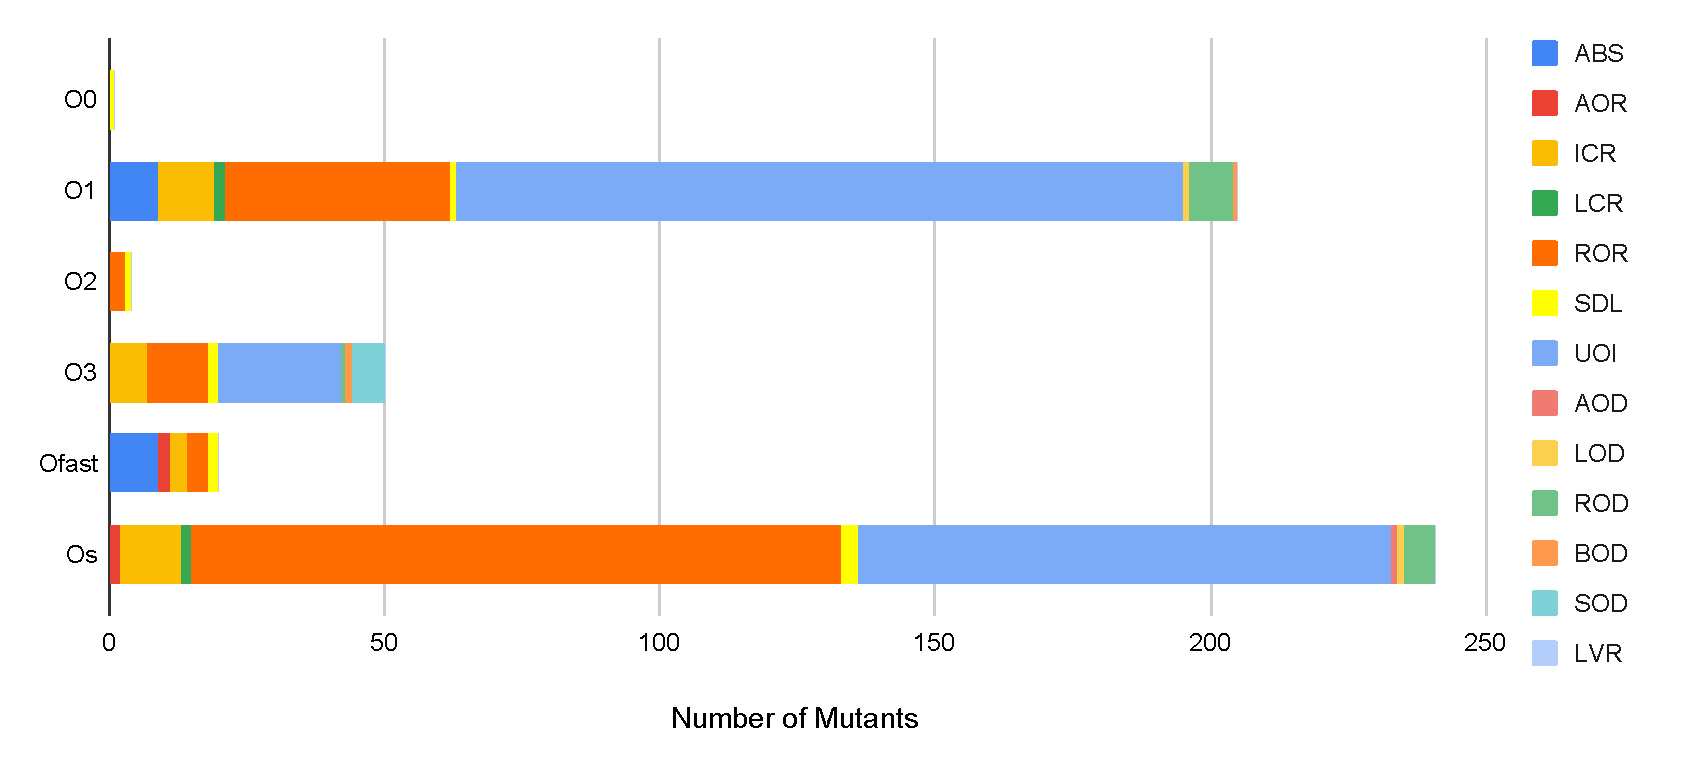
\includegraphics[width=9cm]{images/univ-eq}
\caption{Univocal, Trivially Equivalent Mutants detected by Compiler Optimizations.}
\label{fig:results:univeq}
\end{center}
\end{figure}

\begin{figure}[tb]
\begin{center}
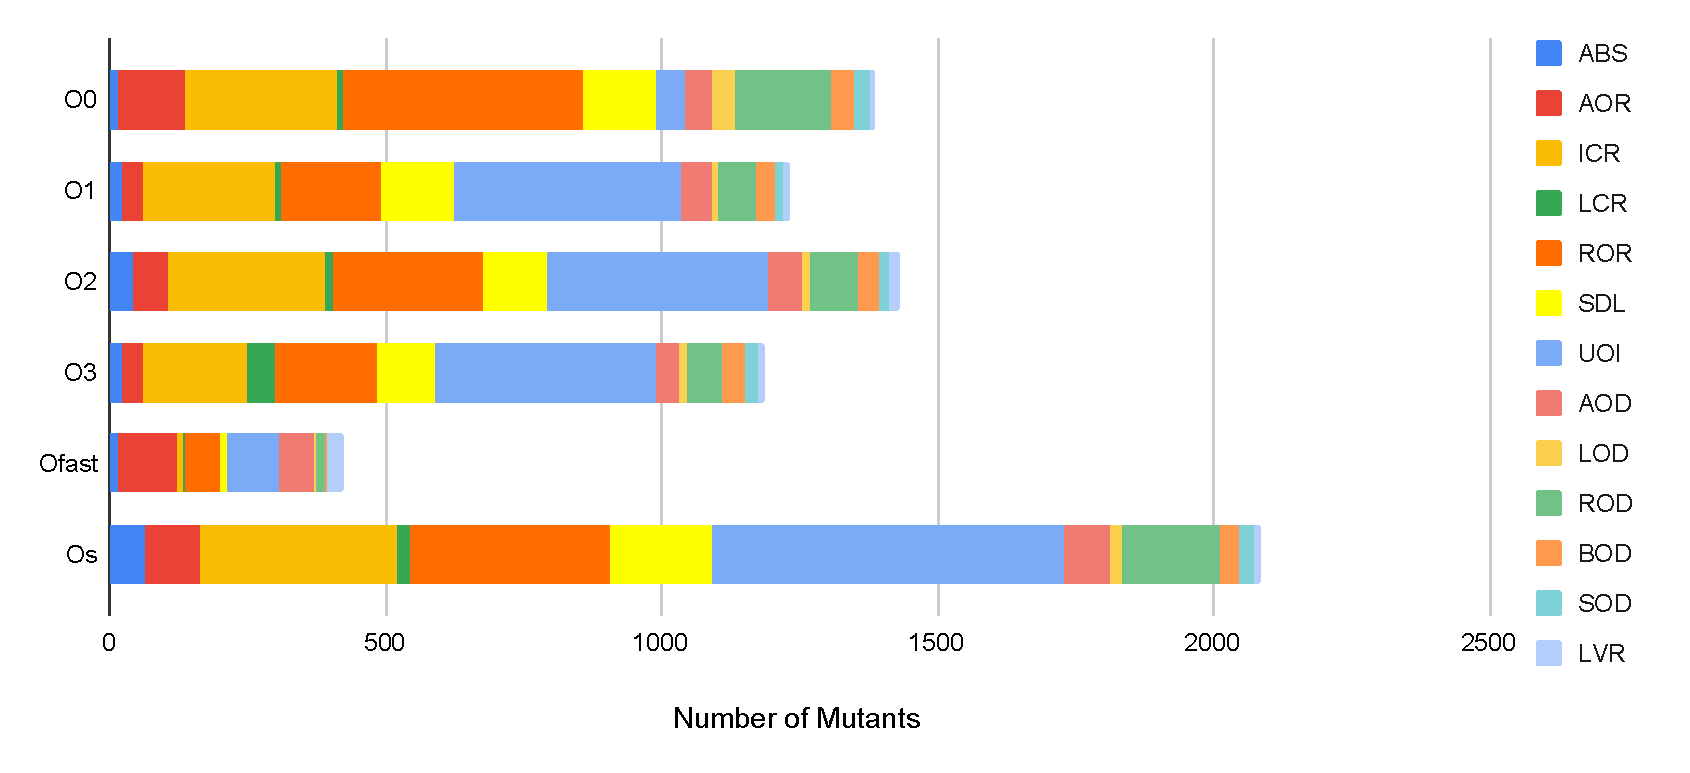
\includegraphics[width=9cm]{images/univ-red}
\caption{Univocal, Trivially Duplicate Mutants detected by Compiler Optimizations.}
\label{fig:results:univred}
\end{center}
\end{figure}




Table~\ref{table:results:compilerOptimizationsTime} provides the time required to compile the artifacts with the different optimization levels. Different from related work, which reports that optimization levels, in the worst case, lead an increase in compilation time by a factor of 5, \textbf{we do not observe a large difference in compilation time among the different optimization levels}. Indeed, in the worst case (i.e., option \emph{-Os}) this factor is $1.1$, an increase of 10\%. This directly results from the \APPR compilation pipeline, which minimizes the number of source files that need to be compiled. If developers can accept a compilation time increased by a factor of 5, as suggested in related work, all the compilation optimization levels can be applied, thus maximizing the number of equivalent and duplicate mutants being detected. In three out of five subjects, it takes less than a day to compile all the mutants with all the available optimization levels, which is acceptable, given the cost saved in subsequent steps. For the cases in which it may take multiple days, our practical solution consists in executing the compilation of the various mutants in parallel (e.g., on Cloud systems); for example, our toolset includes scripts to parallelize mutants compilation on HPC and cloud platforms. In the case of \SAIL{}\emph{-CSW}, the parallel compilation of 142,763 mutants, with the four available compilation options, can be performed in ~90 minutes using 100 nodes.



\subsection{RQ2 - Accuracy of Mutant Sampling Methods}
\label{sec:RQ2}
\subsubsection{Design and measurements}


RQ2 aims to investigate  
%the validity of the findings reported by Zhang et al.~\cite{zhang2013operator} and, which concluded that 
to what extent the mutation score computed from a sample of mutants (hereafter, \INDEX{estimated mutation score}) accurately estimates the mutation score of the complete set of mutants (hereafter, \INDEX{actual mutation score}).

In our study, we consider the sampling strategies which are part of \APPR, as justified earlier: \INDEX{proportional uniform sampling}, \INDEX{proportional method-based sampling},  \INDEX{uniform fixed-size sampling}, and \INDEX{uniform FSCI sampling}. 


Because of the complexity and size of space software, combined with its high test execution cost, we are interested in selecting a very small subset of mutants. 
For this reason, 
to evaluate  \INDEX{proportional uniform sampling} and \INDEX{proportional method-based sampling},
we consider sampling ratios ranging from $1\%$ to $10\%$, in steps of $1\%$. Further,
 %to compare our results with those of Zhang et al., 
 we also cover the range 10\% to 100\%, in steps of $10\%$. To evaluate  \INDEX{uniform fixed-size sampling}, consistent with our earlier discussion, we consider a number of mutants in the range 100 to 1000, in steps of $100$.
Finally, to evaluate \INDEX{proportional method-based sampling}, we consider a threshold for the confidence interval (i.e., $T_{\mathit{CI}}$) that ranges from $0.05$ to $0.10$, in steps of $0.01$, with a confidence level of $95\%$, which is a common choice. The experiments conducted to address RQ2 entail the execution of the entire test suite for every sampled mutant. Executions with a prioritized and reduced test suite are addressed in Section~\ref{exp:accuracy:prioritize}. The evaluation of different values for $T_{\mathit{CI}}$ enable us to determine the costs associated with a more accurate estimation of the mutation score, in order to better understand the trade-offs.


We compute the actual mutation score of each system by executing the test suite against all the mutants that were successfully compiled, excluding mutants detected as being equivalent or duplicate by simple compiler optimization techniques (see RQ1). 
For each sampling ratio, to account for randomness,
we repeat the analysis 100 times, i.e., we compute the mutation score 100 times, based on 100 randomly selected subsets of mutants.
%we randomly select 100 subsets of mutants and compute their mutation score. 
Since it is not feasible to test all the mutants generated for \SAIL{}\emph{-CSW}, as discussed above, we focus on $\mathit{\SAIL{}}_{S}$.



%
%Computation in R: 
%X = set of 100 mutation scores
%quantile(X, c(.025, .975))

% s = standard deviation = sd(X)
% true_score = true mutation score
%z.test(X, sigma.x=s, mu=true_score)
%t.test(X, mu=true_score)
%
Our goal is to determine if the estimated mutation score is an accurate estimate of the actual mutation score.
This happens when the estimated mutation score differs from the actual mutation score for less than a small delta (hereafter, accuracy delta, $\delta_{acc}$) for a large percentage of the runs (e.g., 95\%).
We thus study the distribution of the difference between the estimated and actual mutation scores across all runs. More precisely, we estimate the 2.5\% and 97.5\% quantiles\footnote{We rely on linear interpolation using the type 8 
algorithm suggested in Hyndman and Fan~\cite{Hyndman1996}. It does not make assumptions about the underlying distribution.}.
Since these two quantiles delimit 95\% of the population,
we consider the mutation scores to be accurately estimated when they are within a pre-defined small range of the actual score [$-\delta_{acc}$;$+\delta_{acc}$].
In other words, we consider the estimated mutation score to be accurate when 
%the largest absolute value for the two quantiles is below $\delta_{acc}$.
the absolute value of the largest difference between quantiles and the actual score is below $\delta_{acc}$.
Since the range of acceptable mutation score values is small (75\%-100\%, see Section~1.2.1.1 from D2), we decided to use a threshold of 5\%, which is more conservative than that reported in related work ~\cite{gopinath2015hard}. 

Below, we analyze $\delta_{acc}$ for varying sampling rates. To improve readability, we discuss the results concerning the different sampling strategies separately.
% \emph{proportional uniform sampling} and \emph{proportional method-based sampling}.

% (i.e., the max difference between the actual mutation score and either the 2.5\% quantile or the 97.5\% quantile is below 0.01).

%%Since mutants are selected in random order and their result do not depend on the order in which they are executed, they can be treated as  independent from each other. 
%%We thus perform a t-test (alpha = 0.05) to test if the null hypothesis \emph{the mean mutation score of the sampled subset of mutants is equal to the true mutation score}, is rejected.


\subsubsection{Results - proportional uniform sampling}

%\begin{figure}[tb]
%\begin{center}
%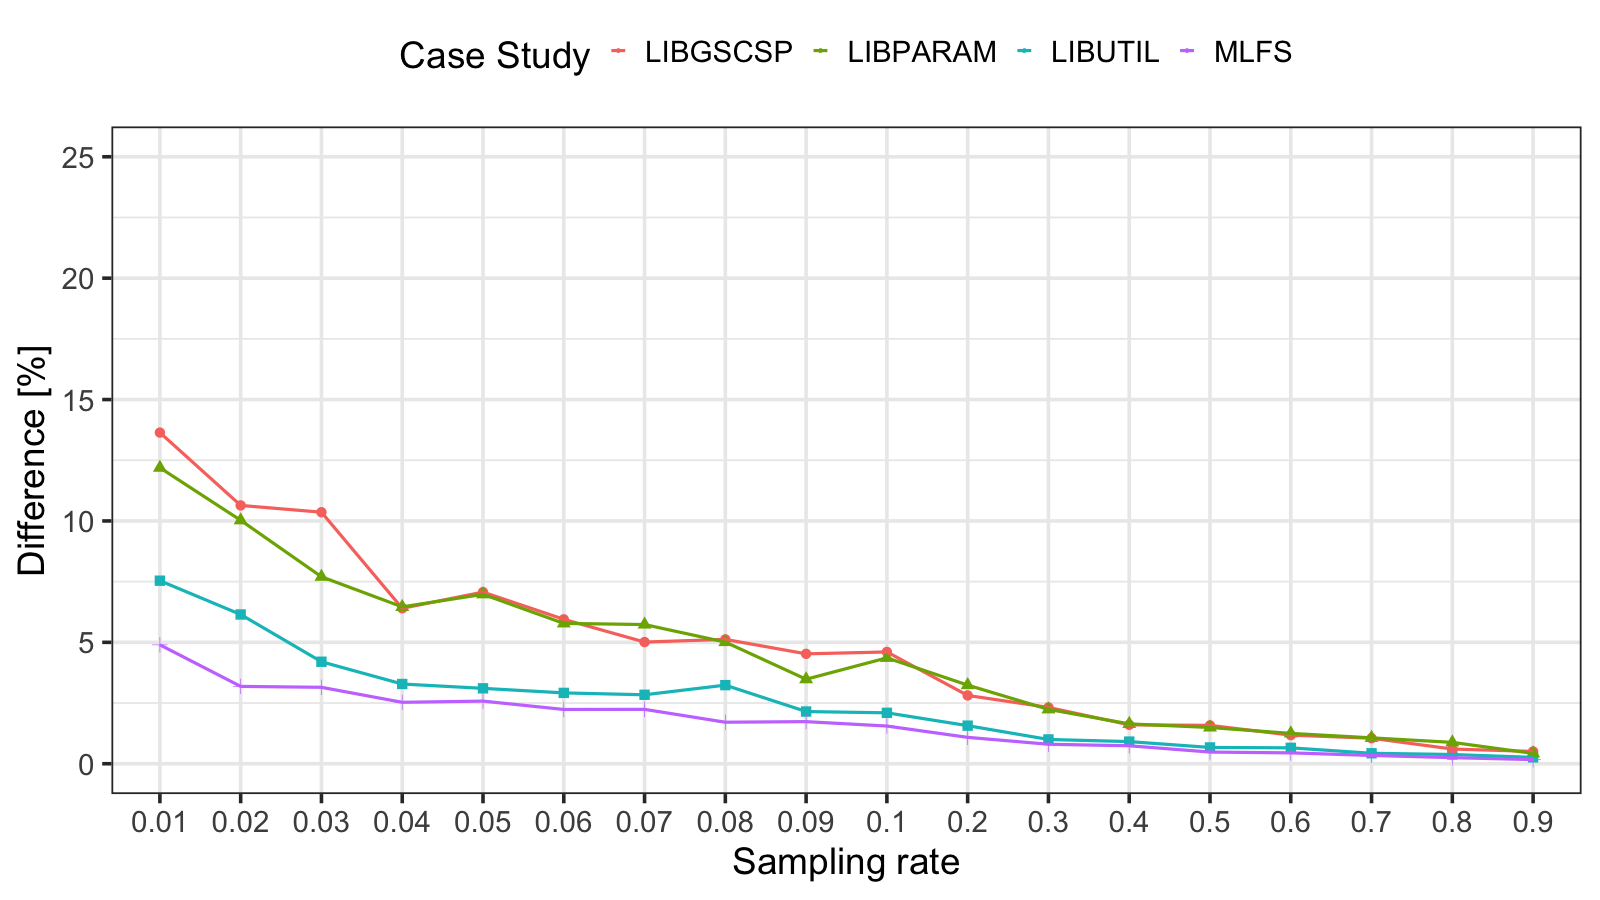
\includegraphics[width=9cm]{images/sampling_regular}
%\caption{Difference between estimated and actual mutation score (i.e., $\delta_{acc}$) for random sampling with different sampling rates.}
%\label{fig:approach}
%\end{center}
%\end{figure}
%
%\begin{figure}[tb]
%\begin{center}
%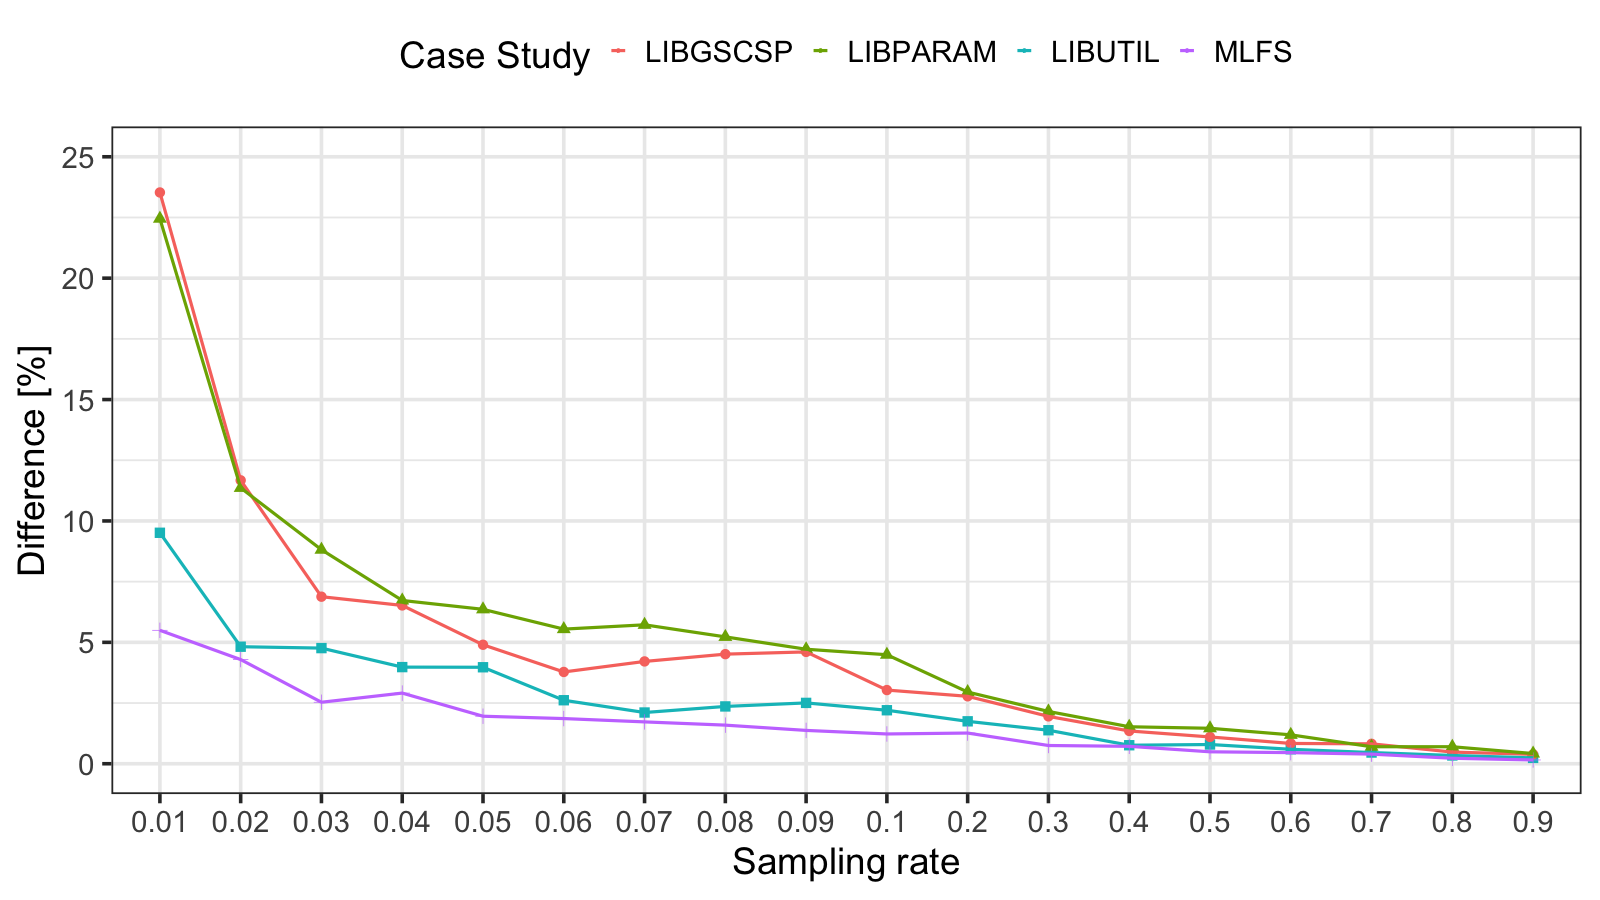
\includegraphics[width=9cm]{images/sampling_func}
%\caption{}
%\label{fig:results:sampling_func}
%\end{center}
%\end{figure}

% !TEX root =  ../Main.tex

\begin{table}[htb]
\caption{Actual mutation scores for artifacts.}
\label{table:results:accuracy:full} 
\scriptsize
\centering
\begin{tabular}{|
@{\hspace{1pt}}p{15mm}|
@{\hspace{1pt}}>{\raggedleft\arraybackslash}p{10mm}@{\hspace{1pt}}|
>{\raggedleft\arraybackslash}p{7mm}@{\hspace{1pt}}|
>{\raggedleft\arraybackslash}p{7mm}@{\hspace{1pt}}|
 >{\raggedleft\arraybackslash}p{25mm}@{\hspace{1pt}}|
}
\hline
\textbf{Case Study}&\textbf{Mutants}&\textbf{Killed}&\textbf{Live}&\textbf{Mutation Score (\%)}\\ 
\hline
$\mathit{ESAIL}_{S}$ &  &  &  &\\
$\mathit{LIBUTIL}$ &20261 & 13590 & 6671 & 71.20 \\
$\mathit{LIBPARAM}$&6435&4291&2144&69.12 \\
$\mathit{LIBGSCSP}$&7878&4905&2973&65.64 \\
$\mathit{MLFS}$&28069&22523&5546&81.80 \\
\hline
\end{tabular}

\end{table}
% !TEX root =  ../Main.tex

\begin{table}[htb]
\caption{RQ2. Accuracy of proportional uniform sampling.}
\label{table:results:accuracy:regSampling} 
\scriptsize
\centering
\begin{tabular}{|
@{\hspace{1pt}}p{5mm}|
@{\hspace{1pt}}>{\raggedleft\arraybackslash}p{7mm}@{\hspace{1pt}}|
>{\raggedleft\arraybackslash}p{5mm}@{\hspace{1pt}}|
>{\raggedleft\arraybackslash}p{6mm}@{\hspace{1pt}}|
 >{\raggedleft\arraybackslash}p{5mm}@{\hspace{1pt}}|
  >{\raggedleft\arraybackslash}p{6mm}@{\hspace{1pt}}|
@{\hspace{1pt}}>{\raggedleft\arraybackslash}p{5mm}@{\hspace{1pt}}|
@{\hspace{1pt}}>{\raggedleft\arraybackslash}p{7mm}@{\hspace{1pt}}|
>{\raggedleft\arraybackslash}p{5mm}@{\hspace{1pt}}|
 >{\raggedleft\arraybackslash}p{8mm}@{\hspace{1pt}}|
  >{\raggedleft\arraybackslash}p{5mm}@{\hspace{1pt}}|
}
\hline
     & \multicolumn{2}{c|}{\textbf{LIBGSCSP}} & \multicolumn{2}{c|}{\textbf{LIBPARAM}} & \multicolumn{2}{c|}{\textbf{LIBUTIL}} & \multicolumn{2}{c|}{\textbf{MLFS}} & \multicolumn{2}{c|}{\textbf{ESAIL}} \\
\hline
\textbf{r=} & \textbf{\#M}&\textbf{$\delta_{acc}$}& \textbf{\#M}&\textbf{$\delta_{acc}$}& \textbf{\#M}&\textbf{$\delta_{acc}$}& \textbf{\#M}&\textbf{$\delta_{acc}$}& \textbf{\#M}&\textbf{$\delta_{acc}$}               \\
\hline
0.01 & 50 & 13.64    			 & 40 & 12.19    			& 146 & 7.54    		& 214 & \textbf{4.90} &   36    & 14.04\\
0.02 & 100 & 10.64    			 & 79 & 10.03    			& 292 & 6.15    		& 428 & \textbf{3.19} &   71    & 11.84\\
0.03 & 150 & 10.36   			 & 118 & 7.70     			& 438 & \textbf{4.20}    & 642 & \textbf{3.15} &   107    & 8.84\\
0.04 & 200 & 6.40     			 & 158 & 6.46     			& 583 & \textbf{3.28}    & 855 & \textbf{2.53} &   142    & 7.92 \\
0.05 & 250 & 7.07     			 & 197 & 6.98     			& 729 & \textbf{3.11}    & 1069 & \textbf{2.58} &  177 & 6.39 \\
0.06 & 299 & 5.95    		 	 & 236 & 5.78     			& 875 & \textbf{2.92}    & 1283 & \textbf{2.24} & 213      &  6.25\\
0.07 & 349 & 5.01     			 & 276 & 5.73     		    & 1021 & \textbf{2.84}    & 1497 & \textbf{2.24} &  248     & 5.20 \\
0.08 & 399 & 5.12    		     & 315 & 5.01 		    	& 1166 & \textbf{3.24}    & 1710 & \textbf{1.71} &  283     & 5.68\\
0.09 & 449 & \textbf{4.53}     	 & 354 & \textbf{3.48}      & 1312 & \textbf{2.15}    & 1924 & \textbf{1.73} &  319     & \textbf{4.55}\\
0.10  & 499 & \textbf{4.61}      & 394 & \textbf{4.36}      & 1458 & \textbf{2.10}    & 2138 & \textbf{1.55} &  354     & \textbf{5.26}\\
0.20  & 997 & \textbf{2.81}      & 787 & \textbf{3.24}      & 2915 & \textbf{1.57}    & 4275 & \textbf{1.09} &    708   & \textbf{3.52}\\
0.30  & 1495 & \textbf{2.32}     & 1180 & \textbf{2.24}     & 4373 & \textbf{1.00}    & 6413 & \textbf{0.80} &  1061 & \textbf{2.56}\\
0.40  & 1993 & \textbf{1.60}     & 1573 & \textbf{1.64}     & 5830 & \textbf{0.91}    & 8550 & \textbf{0.74} &  1415 & \textbf{2.04}\\
0.50  & 2491 & \textbf{1.58}     & 1965 & \textbf{1.49}     & 7287 & \textbf{0.67}    & 10688 & \textbf{0.48} & 1768  & \textbf{1.50}\\
0.60  & 2990 & \textbf{1.18}     & 2358 & \textbf{1.25}     & 8745 & \textbf{0.66}    & 12825 & \textbf{0.45} & 2122  & \textbf{1.28}\\
0.70  & 3488 & \textbf{1.05}     & 2750 & \textbf{1.07}     & 10202 & \textbf{0.43}    & 14963 & \textbf{0.34} & 2476   & \textbf{1.16}\\
0.80  & 3986 & \textbf{0.61}     & 3143 & \textbf{0.88}     & 11660 & \textbf{0.38}    & 17100 & \textbf{0.25} & 2829   & \textbf{0.92}\\
0.90  & 4484 & \textbf{0.51}     & 3534 & \textbf{0.43}     & 13117 & \textbf{0.26}   & 19238 & \textbf{0.17} & 3183& \textbf{0.55}\\
\hline 
\end{tabular}

Note: \#M, number of mutants. Accurate results (i.e., $\delta_{acc} \le 5\%$) are in bold.
\end{table}

\begin{table}[htb]
\caption{RQ2. Accuracy of proportional method-based sampling.}
\label{table:results:accuracy:methodBased} 
\scriptsize
\centering
\begin{tabular}{|
@{\hspace{1pt}}p{5mm}|
@{\hspace{1pt}}>{\raggedleft\arraybackslash}p{7mm}@{\hspace{1pt}}|
>{\raggedleft\arraybackslash}p{5mm}@{\hspace{1pt}}|
>{\raggedleft\arraybackslash}p{6mm}@{\hspace{1pt}}|
 >{\raggedleft\arraybackslash}p{5mm}@{\hspace{1pt}}|
  >{\raggedleft\arraybackslash}p{6mm}@{\hspace{1pt}}|
@{\hspace{1pt}}>{\raggedleft\arraybackslash}p{5mm}@{\hspace{1pt}}|
@{\hspace{1pt}}>{\raggedleft\arraybackslash}p{7mm}@{\hspace{1pt}}|
>{\raggedleft\arraybackslash}p{5mm}@{\hspace{1pt}}|
 >{\raggedleft\arraybackslash}p{8mm}@{\hspace{1pt}}|
  >{\raggedleft\arraybackslash}p{5mm}@{\hspace{1pt}}|
}
\hline
     & \multicolumn{2}{c|}{\textbf{LIBGSCSP}} & \multicolumn{2}{c|}{\textbf{LIBPARAM}} & \multicolumn{2}{c|}{\textbf{LIBUTIL}} & \multicolumn{2}{c|}{\textbf{MLFS}} & \multicolumn{2}{c|}{\textbf{ESAIL}} \\
\hline
\textbf{r=} & \textbf{\#M}&\textbf{$\delta_{acc}$}& \textbf{\#M}&\textbf{$\delta_{acc}$}& \textbf{\#M}&\textbf{$\delta_{acc}$}& \textbf{\#M}&\textbf{$\delta_{acc}$}& \textbf{\#M}&\textbf{$\delta_{acc}$}               \\
\hline
0.01 & 19 & 23.53    			 & 15 & 22.45    			& 111 & 9.51    		 & 232 & 5.50 &  33& 13.84\\
0.02 & 75 & 11.67    			 & 77 & 11.36    			& 250 & \textbf{4.82}    & 447 & \textbf{4.29} &64& 16.18\\
0.03 & 131 & 6.88    			 & 120 & 8.82    			 & 422 & \textbf{4.76}   & 661 & \textbf{2.53} &104   &8.63\\
0.04 & 194 & 6.52    			 & 165 & 6.73    			 & 564 & \textbf{3.98}   & 881 & \textbf{2.91} &137 &9.93\\
0.05 & 258 & \textbf{4.90}     & 208 & 6.36     			& 731 & \textbf{3.97}    & 1094 & \textbf{1.96} &178   &6.84\\
0.06 & 312 & \textbf{3.78}     & 254 & 5.54     			& 905 & \textbf{2.62}    & 1306 & \textbf{1.86} &223& 6.18\\
0.07 & 368 & \textbf{4.21}     & 290 & 5.72     			& 1045 & \textbf{2.11}    & 1517 & \textbf{1.72} &254& 5.72\\
0.08 & 417 & \textbf{4.51}     & 335 & 5.22     			& 1197 & \textbf{2.36}    & 1733 & \textbf{1.59} & 287&\textbf{4.67}\\
0.09 & 466 & \textbf{4.61}     & 378 & \textbf{4.72}    	 & 1353 & \textbf{2.51}    & 1942 & \textbf{1.37} & 331      &\textbf{4.59}\\
0.1  & 515 & \textbf{3.03}     & 413 & \textbf{4.49}     	& 1512 & \textbf{2.20}    & 2159 & \textbf{1.23} &364&\textbf{3.87}\\
0.2  & 1030 & \textbf{2.78}     & 811 & \textbf{2.95}     	& 2963 & \textbf{1.75}    & 4295 & \textbf{1.26} & 721  & \textbf{2.95}\\
0.3  & 1523 & \textbf{1.95}     & 1210 & \textbf{2.15}     & 4446 & \textbf{1.38}    & 6430 & \textbf{0.75} & 1079&\textbf{2.76}\\
0.4  & 2045 & \textbf{1.35}     & 1605 & \textbf{1.52}     & 5942 & \textbf{0.76}    & 8576 & \textbf{0.72} & 1432&\textbf{1.81}\\
0.5  & 2518 & \textbf{1.10}     & 1985 & \textbf{1.46}     & 7361 & \textbf{0.79}    & 10702 & \textbf{0.49} & 1779&\textbf{1.42}\\
0.6  & 3035 & \textbf{0.84}     & 2395 & \textbf{1.19}     & 8853 & \textbf{0.60}    & 12863 & \textbf{0.46} & 2139&\textbf{1.22}\\
0.7  & 3550 & \textbf{0.82}     & 2791 & \textbf{0.70}     & 10334 & \textbf{0.46}    & 15007 & \textbf{0.40} & 2494&\textbf{1.03}\\
0.8  & 4027 & \textbf{0.48}     & 3178 & \textbf{0.70}     & 11779 & \textbf{0.34}    & 17134 & \textbf{0.23} & 2849&\textbf{0.86}\\
0.9  & 4527 & \textbf{0.39}     & 3574 & \textbf{0.42}     & 13228 & \textbf{0.24}    & 19272 & \textbf{0.16} & 3202&\textbf{0.62}\\
\hline
\end{tabular}

Note: \#M, number of mutants. Accurate results (i.e., $\delta_{acc} \le 5\%$) are in bold.
\end{table}




Table~\ref{table:results:accuracy:full} reports on the mutation scores obtained with the entire test suite for all subjects. 
As expected, the best mutation score is obtained for \MLFS{}{}, whose test suite achieves MC/DC coverage. \REVNOV{PTCR-20}{In this project, based on related work, we assume a good quality test suite to have a mutation score above 75\%. However, the objective of this report is not to evaluate the quality of the provided test suites based on the observed mutation score but to evaluate the approach for estimating the mutation score. A discussion of of the quality of the provided test suites based on the mutation score is an activity that might be left for later stages when the mutation testing approach is completed and partners had time to inspect live mutants. Indeed,
 there are a number of factors that affect the computed mutation score; for example, the presence of equivalent mutants lead to live mutants and, consequently, make the mutation score (erroneously) low. The inspection of equivalent mutants for the case studies is till ongoing, at this stage. Also, the reasons for not achieving a high mutation score may vary from case study to case study and needs an in depth investigation. For example, for GSL case studies, this seems to be related to a number of off-the-shelf components integrated in the source of the system. Such off-the-shelf-components are not expected to be tested by the test suite. A mutation score based on only non off-the-shelf-components will be computed in later stages of the project.}

%Figure~\ref{fig:results:accuracy:sampling}  reports a plot with the maximum absolute value of the difference...
Table~\ref{table:results:accuracy:regSampling} provides accuracy results (column $\delta_{acc}$) for proportional uniform sampling for a range of sampling rates~($r$). 
To enable comparisons across sampling methods, Column \emph{\#M} reports the number of mutants sampled for each sampling rate.
As expected, a larger sampling rate leads to more accurate results (i.e., low $\delta_{acc}$). 
We notice that for test suites that ensure MC/DC coverage (i.e., \MLFS{}{}), even a very small sampling ratio (i.e., 0.01) guarantees a $\delta_{acc}$ below 5\%. However, to achieve an accurate mutation score estimate across all subjects, a minimum sampling rate of 0.09 is required.

%Table~\ref{table:results:accuracy:sampling} reports, for every case study system, sampling strategy, and sampling ratio, the max difference between the actual mutation score and either the 2.5\%/97.5\% quantile.

%\FIXME{... We cannot go much below 5\%, but in certain systems 5\% is still a lot.}

In addition, we observe that, for $r=0.09$, the worst results (highest deltas) are observed for smaller projects, which indicates that \textbf{the estimation accuracy may not depend on the percentage of sampled mutants but on the size of the sample}; indeed, for most of the subjects, accurate results \CHANGED{(i.e., $\delta_{acc} < 5\%$)} are obtained with a number of mutants between 350 and 450. This aspect is further studied when considering  \INDEX{uniform fixed-size sampling} and \INDEX{uniform FSCI sampling}.

\subsubsection{Results - proportional method-based sampling}

Table~\ref{table:results:accuracy:methodBased} shows the accuracy results for proportional method-based sampling. 
Interestingly, for two subjects (i.e., \GCSP{} and \UTIL{}), proportional method-based sampling leads to accurate estimates of the mutation score with a lower number of mutants than proportional uniform sampling (i.e., around 250).
However, to achieve accurate results with all subjects, we need a minimal sampling rate of $r=0.09$, as for proportional uniform sampling, which, in the case of method-based sampling, leads to a slightly higher number of mutants. For this reason, we do not see any benefit in using method-based sampling.




\subsubsection{Results - uniform fixed-size sampling, uniform FSCI sampling}

%\begin{figure}[tb]
%\begin{center}
%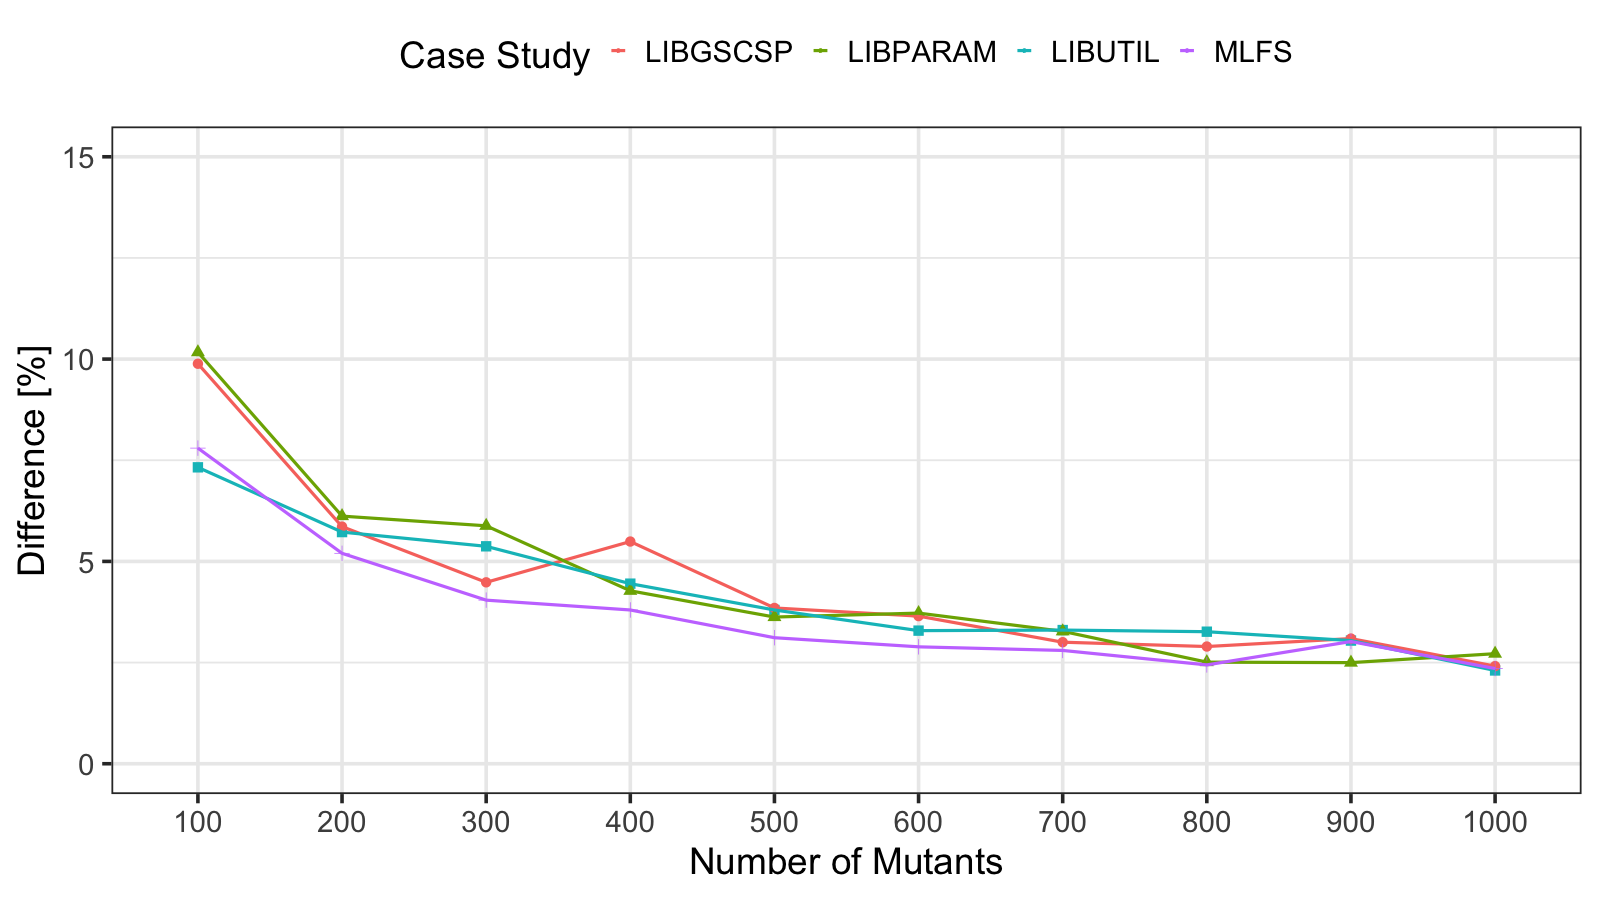
\includegraphics[width=6cm]{images/sampling_fixed}
%\caption{}
%\label{fig:results:fixedNumberOfMutants}
%\end{center}
%\end{figure}
% !TEX root =  ../Main.tex

\begin{table*}[htb]
\caption{RQ2. Accuracy with uniform fixed-size sampling and uniform FSCI sampling. }
\label{table:results:accuracy:FSCI:sampling} 
\scriptsize
\centering
\begin{tabular}{|
>{\raggedleft\arraybackslash}p{10mm}@{\hspace{1pt}}|
>{\raggedleft\arraybackslash}p{5mm}@{\hspace{1pt}}|
p{12mm}@{\hspace{1pt}}|
>{\raggedleft\arraybackslash}p{10mm}@{\hspace{1pt}}|
>{\raggedleft\arraybackslash}p{5mm}@{\hspace{1pt}}|
p{12mm}@{\hspace{1pt}}|
>{\raggedleft\arraybackslash}p{10mm}@{\hspace{1pt}}|
>{\raggedleft\arraybackslash}p{5mm}@{\hspace{1pt}}|
p{12mm}@{\hspace{1pt}}|
>{\raggedleft\arraybackslash}p{10mm}@{\hspace{1pt}}|
>{\raggedleft\arraybackslash}p{5mm}@{\hspace{1pt}}|
p{12mm}@{\hspace{1pt}}|
>{\raggedleft\arraybackslash}p{10mm}@{\hspace{1pt}}|
>{\raggedleft\arraybackslash}p{5mm}@{\hspace{1pt}}|
p{12mm}@{\hspace{1pt}}|
}
\hline
\multicolumn{3}{|c|}{\textbf{LIBGSCSP}}      & \multicolumn{3}{c|}{\textbf{LIBPARAM}}      & \multicolumn{3}{c|}{\textbf{LIBUTIL}}       & \multicolumn{3}{c|}{\textbf{MLFS}}          & \multicolumn{3}{c|}{\textbf{ESAIL}}       \\
\hline
\textbf{\#Mutants} & $\delta_{acc}$ & \textbf{Method}   & \textbf{\#Mutants} & $\delta_{acc}$ & \textbf{Method}   & \textbf{\#Mutants} & $\delta_{acc}$ & \textbf{Method}   & \textbf{\#Mutants} & $\delta_{acc}$ & \textbf{Method}   & \textbf{\#Mutants} & $\delta_{acc}$ & \textbf{Method} \\
\hline
100       & 9.88       & FIXED    & 100       & 10.17      & FIXED    & 100       & 7.32       & FIXED    & 100       & 7.80       & FIXED    &  100         &     8.89       &   FIXED     \\
200       & 5.86       & FIXED    & 200       & 6.12       & FIXED    & 200       & 5.73       & FIXED    & 200       & 5.20       & FIXED    &   200        &      6.14      &   FIXED     \\
300       & \textbf{4.48}       & FIXED    & 300       & 5.88       & FIXED    & 300       & 5.37       & FIXED    & 248       & \textbf{4.56}       & CI 0.1  &    300       &      5.53      &    FIXED    \\
364       & \textbf{4.42}       & FSCI 0.1  & 346       & \textbf{4.26}       & FSCI 0.1  & 333       & \textbf{4.73}       & FSCI 0.1  & 300       & \textbf{4.04}       & FIXED    &   366        &     \textbf{3.92}       &    FSCI 0.1    \\
400       & \textbf{5.49}       & FIXED    & 400       & \textbf{4.27}       & FIXED    & 400       & \textbf{4.45}       & FIXED    & 302       & \textbf{4.64}       & FSCI 0.09 &     400      &     \textbf{4.52}       &    FIXED    \\
447       & \textbf{3.70}       & FSCI 0.09 & 425       & \textbf{3.79}       & FSCI 0.09 & 409       & \textbf{4.08}       & FSCI 0.09 & 379       & \textbf{4.01}       & FSCI 0.08 &   449        &    \textbf{3.66}     &   FSCI 0.09    \\
500       & \textbf{3.85}       & FIXED    & 500       & \textbf{3.63}       & FIXED    & 500       & \textbf{3.80}       & FIXED    & 400       & \textbf{3.80}       & FIXED    &   500      &      \textbf{4.08}      &   FIXED     \\
564       & \textbf{3.53}       & FSCI 0.08 & 536       & \textbf{3.75}       & FSCI 0.08 & 514       & \textbf{3.94}       & FSCI 0.08 & 490       & \textbf{3.90}       & FSCI 0.07 &    567       &  \textbf{3.03}   &  FSCI 0.08      \\
600       & \textbf{3.65}       & FIXED    & 600       & \textbf{3.72}       & FIXED    & 600       & \textbf{3.29}       & FIXED    & 500       & \textbf{3.11}       & FIXED    &     600      &  \textbf{3.73}          &     FIXED   \\
700       & \textbf{3.00}       & FIXED    & 696       & \textbf{2.89}       & FSCI 0.07 & 668       & \textbf{3.99}       & FSCI 0.07 & 600       & \textbf{2.89}       & FIXED    &     700      &      \textbf{3.01}      &    FIXED    \\
734       & \textbf{3.62}       & FSCI 0.07 & 700       & \textbf{3.27}       & FIXED    & 700       & \textbf{3.30}       & FIXED    & 667       & \textbf{2.78}       & FSCI 0.06 &     738      &      \textbf{2.77}      &    FSCI 0.07    \\
800       & \textbf{2.90}       & FIXED    & 800       & \textbf{2.51}       & FIXED    & 800       & \textbf{3.26}       & FIXED    & 700       & \textbf{2.80}       & FIXED    &     800      &  \textbf{2.55}          &    FIXED    \\
900       & \textbf{3.09}       & FIXED    & 900       & \textbf{2.50}       & FIXED    & 900       & \textbf{3.04}       & FIXED    & 800       & \textbf{2.44}       & FIXED    &     900      &  \textbf{2.37}          &    FIXED    \\
994       & \textbf{3.00}       & FSCI 0.06 & 945       & \textbf{2.42}       & FSCI 0.06 & 906       & \textbf{3.28}       & FSCI 0.06 & 900       & \textbf{3.02}       & FIXED    &  998         &  \textbf{2.65}         &   FSCI 0.06     \\
1000      & \textbf{2.41}       & FIXED    & 1000      & \textbf{2.72}       & FIXED    & 1000      & \textbf{2.31}       & FIXED    & 960       & \textbf{2.31}       & FSCI 0.05 & 1000     &  \textbf{2.96}          &   FIXED     \\
1422      & \textbf{2.44}       & FSCI 0.05 & 1352      & \textbf{1.93}       & FSCI 0.05 & 1298      & \textbf{2.72}       & FSCI 0.05 & 1000      & \textbf{2.35}       & FIXED    &    1429     &    \textbf{1.70}        &  FSCI 0.05 \\
\hline
\end{tabular}

Accurate results (i.e., $\delta_{acc} \le 5\%$) are in bold.
\end{table*}

Table~\ref{table:results:accuracy:FSCI:sampling} shows the accuracy results for uniform fixed-size sampling and uniform FSCI sampling. For each subject, we sort results according to the number of mutants. For FSCI sampling, we report the confidence interval threshold $T_\mathit{CI}$. 

The best results (i.e., lowest number of mutants with $\delta_{acc} \le 5\%$) are obtained using  FSCI sampling with $T_\mathit{CI}=0.10$. Predictably, FSCI sampling with $T_\mathit{CI}=0.10$ guarantees $\delta_{acc} \le 5\%$ (half of $T_\mathit{CI}$); indeed, by construction, if our assumptions 
on the limited correlation between mutants and the mutation score following a  binomial distribution hold (see Section~1.2.1.4 from D2),
FSCI sampling with $T_\mathit{CI}=0.10$ is expected to guarantee $\delta_{acc} \le 5\%$ (see Appendix
B
%~\ref{appendix:correlation} 
for further details on the distribution of the mutation score across subjects).

In addition, our results suggest that a limited number of mutants (between 300 and 400) is required to achieve the desired $\delta_{acc}$. This sample size is much lower than the (worst case) sample size proposed by Gopinath et al., which is 1,000~\cite{gopinath2015hard}. Also, our sample size is smaller 
than the one estimated, for a mutation score between 60\% and 80\%, by 
approaches
%a priori approaches 
based on confidence-interval estimation, which is still around 1,000~\cite{Goncalves2012}. 
%that could be estimated a priori for a mutation score between 60\% and 80\%, which is around 1,000~\cite{Goncalves2012}. 
However, we confirm the finding of Gopinath et al., who demonstrated that the binomial distribution %provides a conservative estimation of the
accurately estimates the mutation score~\cite{gopinath2015hard}.

To summarize, this is the first study demonstrating that \textbf{FSCI sampling is the 
best approach for obtaining the smallest sample size
%optimal approach for determining sample size 
while providing guarantees on the accuracy of mutation score estimates.} 
We therefore propose a better solution than that of Gopinath et al., who provide an upper bound for the number of mutants to be considered in uniform fixed-size sampling, since we have evidence suggesting that FSCI sampling helps to select a significantly smaller sample size for a desired confidence interval.





\subsection{RQ3 - SDL accuracy}



\subsubsection{Design and measurements}


RQ3 assesses if mutants generated using only deletion operators can accurately estimate the mutation score of the complete mutants set.

To this end, we study the difference between the mutation score obtained by executing the entire test suite on the mutants generated with all the operators (i.e., the actual mutation score) and the mutation score obtained with either (1) the mutants generated with the SDL operator only, or (2) the mutants generated with both the SDL and OODL operators.
As for RQ2, to be accurate, the mutation score obtained with a subset of operators should differ by at most 5\%.


\subsubsection{Results}

% !TEX root =  ../Main.tex

\begin{table}[htb]
\caption{Comparison of mutation scores obtained with mutants generated using all operators, the SDL operator only, and the SDL + OODL operators.}
\label{table:results:score:sdl:oodl} 
\scriptsize
\centering
\begin{tabular}{|
@{\hspace{1pt}}p{15mm}|
 >{\raggedleft\arraybackslash}p{8mm}@{\hspace{1pt}}|
  >{\raggedleft\arraybackslash}p{13mm}@{\hspace{1pt}}|
 >{\raggedleft\arraybackslash}p{6mm}@{\hspace{1pt}}|
  >{\raggedleft\arraybackslash}p{15mm}@{\hspace{1pt}}|
   >{\raggedleft\arraybackslash}p{15mm}@{\hspace{1pt}}|
}
\hline
\textbf{Case Study}&\multicolumn{2}{c|}{\textbf{\# Mutants}}&\multicolumn{3}{c|}{\textbf{Mutation score}}\\ 
&SDL&SDL+OODL&ALL&SDL&SDL+OODL\\
\hline
$\mathit{ESAIL}_{S}$ &	701&	974& 65.36 & 61.91 (-3.45) & 63.45 (-1.91) \\
$\mathit{LIBGSCSP}$ & 912	&1546	&65.64 &70.72 (+5.08) &71.35 (+5.71)\\
$\mathit{LIBPARAM}$ & 731&1324	&69.12 &64.84 (-4.28) &66.39 (+2.73)\\
$\mathit{LIBUTIL}$ 	 &2341	&3811	&71.20 & 73.26 (+2.06) &72.63 (+1.43)\\
$\mathit{MLFS}$ &1729	&	5971	&81.80 &85.71 (3.91)& 88.03 (+6.23)\\
\hline
\end{tabular}

\end{table}

In Table~\ref{table:results:score:sdl:oodl}, column \emph{\# Mutants} shows, for each subject, the number of mutants generated with either the SDL operator or both the SDL and OODL operators. 
Column \emph{Mutation score} shows the mutation score obtained when using the entire test suite to exercise the mutants generated with either all the operators, the SDL operator only, or both the SDL and OODL operators. Between parentheses, we also report the difference between the mutation score obtained with all the operators and that obtained with a subset of operators. Results show that, for some of our subjects, the mutation score obtained with the SDL operator does not accurately estimate the mutation score obtained with a broader set of operators. Though these results do not invalidate related work~\cite{delamaro2014experimental}, whose focus is on the evaluation of the strength of SDL and OODL operators, it shows that \textbf{SDL and OODL operators should not be adopted to estimate the mutation score computed with a larger set of operators}. We leave the evaluation of the strength of SDL and OODL operators to future work.




%is always accurate; instead, the mutation score obtained with both the SDL and OODL operators is not accurate in the case of MLFS.}

%Tables~\ref{table:results:accuracy:regSamplingSDL} to~\ref{table:results:accuracy:funcSamplingSDLOODL} show the accuracy of proportional uniform and method-based sampling applied to select mutants generated either with the SDL operator only or with the SDL and OODL operators. 
%Tables~\ref{table:results:accuracy:sampling_sdl} and~\ref{table:results:accuracy:sampling_sdl_oodl} show the accuracy of uniform fixed-size sampling and uniform FSCI sampling applied to select mutants generated either with the SDL operator only or with both the SDL and OODL operators. In all the cases, it is not possible to identify any sampling rate that enable an accurate  (i.e., $\delta_{acc} \le 5\%$) estimation of the mutation score. \FIXME{This is mostly due which might be partially due to the overall number of mutants being generated being low.}
%
%
%\FIXME{We suggest to rely on SDL/SLD+OODL...}

%% !TEX root =  ../Main.tex
\begin{table}[htb]
\caption{RQ3. 
Accuracy of proportional uniform sampling applied to select SDL mutants only.}
\label{table:results:accuracy:regSamplingSDL} 
\scriptsize
\centering
\begin{tabular}{|
@{\hspace{1pt}}p{5mm}|
@{\hspace{1pt}}>{\raggedleft\arraybackslash}p{7mm}@{\hspace{1pt}}|
>{\raggedleft\arraybackslash}p{5mm}@{\hspace{1pt}}|
>{\raggedleft\arraybackslash}p{6mm}@{\hspace{1pt}}|
 >{\raggedleft\arraybackslash}p{5mm}@{\hspace{1pt}}|
  >{\raggedleft\arraybackslash}p{6mm}@{\hspace{1pt}}|
@{\hspace{1pt}}>{\raggedleft\arraybackslash}p{5mm}@{\hspace{1pt}}|
@{\hspace{1pt}}>{\raggedleft\arraybackslash}p{7mm}@{\hspace{1pt}}|
>{\raggedleft\arraybackslash}p{5mm}@{\hspace{1pt}}|
 >{\raggedleft\arraybackslash}p{8mm}@{\hspace{1pt}}|
  >{\raggedleft\arraybackslash}p{5mm}@{\hspace{1pt}}|
}
\hline
     & \multicolumn{2}{c|}{\textbf{LIBGSCSP}} & \multicolumn{2}{c|}{\textbf{LIBPARAM}} & \multicolumn{2}{c|}{\textbf{LIBUTIL}} & \multicolumn{2}{c|}{\textbf{MLFS}} & \multicolumn{2}{c|}{\textbf{ESAIL}} \\
\hline
\textbf{r=} & \textbf{\#M}&\textbf{$\delta_{acc}$}& \textbf{\#M}&\textbf{$\delta_{acc}$}& \textbf{\#M}&\textbf{$\delta_{acc}$}& \textbf{\#M}&\textbf{$\delta_{acc}$}& \textbf{\#M}&\textbf{$\delta_{acc}$}               \\
\hline           
0.01 & 10 & 34.36    & 8 & 38.18     & 24 & 16.30   & 18 & 20.69 &       \\
0.02 & 19 & 23.83    & 15 & 29.12    & 47 & 13.91   & 35 & 15.34 &       \\
0.03 & 28 & 20.07    & 22 & 23.67    & 71 & 14.72   & 52 & 12.43 &       \\
0.04 & 37 & 19.56    & 30 & 20.87    & 94 & 11.27   & 70 & 11.06 &       \\
0.05 & 46 & 18.11    & 37 & 17.77    & 118 & 9.31    & 87 & 10.15 &       \\
0.06 & 55 & 15.32    & 44 & 21.39    & 141 & 9.31    & 104 & 9.09  &       \\
0.07 & 64 & 15.61    & 52 & 16.28    & 164 & 9.64    & 122 & 9.18  &       \\
0.08 & 73 & 13.81    & 59 & 16.58    & 188 & 6.99    & 139 & 9.57  &       \\
0.09 & 83 & 11.53    & 66 & 16.16    & 211 & 8.20    & 156 & 8.28  &       \\
0.1  & 92 & 13.19    & 74 & 15.07    & 235 & 7.97    & 173 & 9.25  &       \\
0.2  & 183 & 10.32    & 147 & 9.94     & 469 & 5.25    & 346 & 6.64  &       \\
0.3  & 274 & 9.91     & 220 & 9.12     & 703 & \textbf{4.91}    & 519 & 7.13  &       \\
0.4  & 365 & 8.48     & 292 & 8.73     & 937 & \textbf{4.43}    & 692 & 6.06  &       \\
0.5  & 456 & 8.07     & 364 & 7.38     & 1171 & \textbf{3.61}    & 865 & 5.60  &       \\
0.6  & 548 & 7.17     & 438 & 7.28     & 1405 & \textbf{3.50}    & 1038 & 5.25  &       \\
0.7  & 639 & 6.90     & 510 & 5.86     & 1639 & \textbf{3.27}    & 1211 & \textbf{4.91}  &       \\
0.8  & 730 & 6.56     & 582 & 5.79     & 1873 & \textbf{2.80}    & 1384 & \textbf{4.87}  &       \\
0.9  & 821 & 5.86     & 655 & 5.22     & 2107 & \textbf{2.58}    & 1557 & \textbf{4.49}  &   \\
\hline   
\end{tabular}
Note: \#M, number of mutants. Accurate results (i.e., $\delta_{acc} \le 5\%$) are in bold.
\end{table}


\begin{table}[htb]
\caption{RQ3. 
Accuracy of proportional method-based sampling applied to select SDL mutants only.}
\label{table:results:accuracy:funcSamplingSDL} 
\scriptsize
\centering
\begin{tabular}{|
@{\hspace{1pt}}p{5mm}|
@{\hspace{1pt}}>{\raggedleft\arraybackslash}p{7mm}@{\hspace{1pt}}|
>{\raggedleft\arraybackslash}p{5mm}@{\hspace{1pt}}|
>{\raggedleft\arraybackslash}p{6mm}@{\hspace{1pt}}|
 >{\raggedleft\arraybackslash}p{5mm}@{\hspace{1pt}}|
  >{\raggedleft\arraybackslash}p{6mm}@{\hspace{1pt}}|
@{\hspace{1pt}}>{\raggedleft\arraybackslash}p{5mm}@{\hspace{1pt}}|
@{\hspace{1pt}}>{\raggedleft\arraybackslash}p{7mm}@{\hspace{1pt}}|
>{\raggedleft\arraybackslash}p{5mm}@{\hspace{1pt}}|
 >{\raggedleft\arraybackslash}p{8mm}@{\hspace{1pt}}|
  >{\raggedleft\arraybackslash}p{5mm}@{\hspace{1pt}}|
}
\hline
     & \multicolumn{2}{c|}{\textbf{LIBGSCSP}} & \multicolumn{2}{c|}{\textbf{LIBPARAM}} & \multicolumn{2}{c|}{\textbf{LIBUTIL}} & \multicolumn{2}{c|}{\textbf{MLFS}} & \multicolumn{2}{c|}{\textbf{ESAIL}} \\
\hline
\textbf{r=} & \textbf{\#M}&\textbf{$\delta_{acc}$}& \textbf{\#M}&\textbf{$\delta_{acc}$}& \textbf{\#M}&\textbf{$\delta_{acc}$}& \textbf{\#M}&\textbf{$\delta_{acc}$}& \textbf{\#M}&\textbf{$\delta_{acc}$}               \\
\hline
0.01 & NA       			& NA       		& 4 & 28.80   			& 4 & 31.80 &       \\
0.02 & NA       			& 2 & 69.12    & 15 & 28.80   			& 20 & 18.20 &       \\
0.03 & 2 & 34.36    		& 8 & 44.12    & 28 & 18.09   			& 35 & 15.34 &       \\
0.04 & 10 & 34.36    		& 9 & 35.79    & 44 & 15.16   			& 76 & 12.94 &       \\
0.05 & 12 & 26.03    		& 9 & 35.79    & 64 & 14.00   			& 88 & 11.98 &       \\
0.06 & 15 & 21.03    		& 19 & 24.51    & 88 & 10.62  			 & 109 & 9.94  &       \\
0.07 & 19 & 18.57    		& 25 & 21.12    & 108 & 10.33  			 & 132 & 8.35  &       \\
0.08 & 25 & 22.36    		& 42 & 19.12    & 135 & 6.97   			 & 146 & 8.61  &       \\
0.09 & 40 & 14.36   		 & 46 & 19.12    & 155 & 8.19   			 & 161 & 8.88  &       \\
0.1  & 56- 11.15     		& 57 & 15.67    & 174 & 8.41    			& 176 & 8.54  &       \\
0.2  & 169 & 7.45     		& 153 & 10.68    & 438 & 5.97    			& 348 & 7.43  &       \\
0.3  & 268 & 7.12     		& 238 & 9.46     & 706 & \textbf{3.17}    & 528 & 6.18  &       \\
0.4  & 370 & 7.60     		& 307 & 8.25     & 948 & \textbf{2.85}    & 703 & 5.40  &       \\
0.5  & 446 & 6.78     		& 377 & 8.01     & 1171 & \textbf{3.57}    & 872 & 5.53  &       \\
0.6  & 559 & 5.38     		& 460 & 6.76     & 1445 & \textbf{2.86}    & 1053 & 5.05  &       \\
0.7  & 653 & 5.26     		& 534 & 6.37     & 1686 & \textbf{2.67}    & 1225 & \textbf{4.45}  &       \\
0.8  & 726 & 5.43     		& 599 & 5.86     & 1899 & \textbf{2.08}    & 1396 & \textbf{4.30}  &       \\
0.9  & 808 & \textbf{4.47}     & 675 & 5.35     & 2120 & \textbf{2.03}    & 1567 & \textbf{4.07}  &   \\
\hline     
\end{tabular}
Note: \#M, number of mutants. Accurate results (i.e., $\delta_{acc} \le 5\%$) are in bold.
\end{table}


\begin{table}[htb]
\caption{RQ3. 
Accuracy of proportional uniform sampling applied to select SDL+OODL mutants only.}
\label{table:results:accuracy:regSamplingSDLOODL} 
\scriptsize
\centering
\begin{tabular}{|
@{\hspace{1pt}}p{5mm}|
@{\hspace{1pt}}>{\raggedleft\arraybackslash}p{7mm}@{\hspace{1pt}}|
>{\raggedleft\arraybackslash}p{5mm}@{\hspace{1pt}}|
>{\raggedleft\arraybackslash}p{6mm}@{\hspace{1pt}}|
 >{\raggedleft\arraybackslash}p{5mm}@{\hspace{1pt}}|
  >{\raggedleft\arraybackslash}p{6mm}@{\hspace{1pt}}|
@{\hspace{1pt}}>{\raggedleft\arraybackslash}p{5mm}@{\hspace{1pt}}|
@{\hspace{1pt}}>{\raggedleft\arraybackslash}p{7mm}@{\hspace{1pt}}|
>{\raggedleft\arraybackslash}p{5mm}@{\hspace{1pt}}|
 >{\raggedleft\arraybackslash}p{8mm}@{\hspace{1pt}}|
  >{\raggedleft\arraybackslash}p{5mm}@{\hspace{1pt}}|
}
\hline
     & \multicolumn{2}{c|}{\textbf{LIBGSCSP}} & \multicolumn{2}{c|}{\textbf{LIBPARAM}} & \multicolumn{2}{c|}{\textbf{LIBUTIL}} & \multicolumn{2}{c|}{\textbf{MLFS}} & \multicolumn{2}{c|}{\textbf{ESAIL}} \\
\hline
\textbf{r=} & \textbf{\#M}&\textbf{$\delta_{acc}$}& \textbf{\#M}&\textbf{$\delta_{acc}$}& \textbf{\#M}&\textbf{$\delta_{acc}$}& \textbf{\#M}&\textbf{$\delta_{acc}$}& \textbf{\#M}&\textbf{$\delta_{acc}$}               \\
\hline
0.01 & 16 & 28.11    & 14 & 26.26    & 39 & 12.23   & 60 & 12.41 &       \\
0.02 & 31 & 21.46    & 27 & 19.21    & 77 & 12.60   & 120 & 10.70 &       \\
0.03 & 47 & 16.33    & 40 & 16.62    & 115 & 10.54   & 180 & 10.42 &       \\
0.04 & 62 & 13.39    & 53 & 11.62    & 153 & 7.88    & 239 & 10.47 &       \\
0.05 & 78 & 14.52    & 67 & 12.40    & 191 & 6.81    & 299 & 9.34  &       \\
0.06 & 93 & 13.93    & 80 & 11.03    & 229 & 6.53    & 359 & 9.71  &       \\
0.07 & 109 & 13.26    & 92 & 9.98     & 267 & 5.97    & 418 & 9.00  &       \\
0.08 & 124 & 11.78    & 106 & 13.01    & 305 & 6.02    & 478 & 8.48  &       \\
0.09 & 140 & 13.68    & 120 & 8.29     & 343 & 5.78    & 538 & 9.00  &       \\
0.1  & 155 & 11.13    & 133 & 9.72     & 382 & 5.38    & 598 & 8.67  &       \\
0.2  & 310 & 10.34    & 265 & 7.99     & 763 & \textbf{3.58}    & 1195 & 7.99  &       \\
0.3  & 464 & 9.04     & 398 & 6.31     & 1144 & \textbf{3.59}    & 1792 & 7.52  &       \\
0.4  & 619 & 8.03     & 529 & 5.54     & 1525 & \textbf{3.26}    & 2389 & 7.03  &       \\
0.5  & 773 & 7.65     & 659 & 5.45     & 1906 & \textbf{2.97}    & 2986 & 7.11  &       \\
0.6  & 928 & 7.48     & 795 & \textbf{4.53}     & 2287 & \textbf{2.41}    & 3583 & 6.90  &       \\
0.7  & 1083 & 7.08     & 926 & \textbf{4.24}     & 2668 & \textbf{2.31}    & 4180 & 6.76  &       \\
0.8  & 1237 & 6.79     & 1058 & \textbf{3.75}     & 3049 & \textbf{2.10}    & 4777 & 6.70  &       \\
0.9  & 1392 & 6.38     & 1189 & \textbf{3.56}     & 3430 & \textbf{1.97}    & 5374 & 6.50  &      \\
\hline 
\end{tabular}
Note: \#M, number of mutants. Accurate results (i.e., $\delta_{acc} \le 5\%$) are in bold.
\end{table}


\begin{table}[htb]
\caption{RQ3. 
Accuracy of proportional method-based sampling applied to select SDL+OODL mutants.}
\label{table:results:accuracy:funcSamplingSDLOODL} 
\scriptsize
\centering
\begin{tabular}{|
@{\hspace{1pt}}p{5mm}|
@{\hspace{1pt}}>{\raggedleft\arraybackslash}p{7mm}@{\hspace{1pt}}|
>{\raggedleft\arraybackslash}p{5mm}@{\hspace{1pt}}|
>{\raggedleft\arraybackslash}p{6mm}@{\hspace{1pt}}|
 >{\raggedleft\arraybackslash}p{5mm}@{\hspace{1pt}}|
  >{\raggedleft\arraybackslash}p{6mm}@{\hspace{1pt}}|
@{\hspace{1pt}}>{\raggedleft\arraybackslash}p{5mm}@{\hspace{1pt}}|
@{\hspace{1pt}}>{\raggedleft\arraybackslash}p{7mm}@{\hspace{1pt}}|
>{\raggedleft\arraybackslash}p{5mm}@{\hspace{1pt}}|
 >{\raggedleft\arraybackslash}p{8mm}@{\hspace{1pt}}|
  >{\raggedleft\arraybackslash}p{5mm}@{\hspace{1pt}}|
}
\hline
     & \multicolumn{2}{c|}{\textbf{LIBGSCSP}} & \multicolumn{2}{c|}{\textbf{LIBPARAM}} & \multicolumn{2}{c|}{\textbf{LIBUTIL}} & \multicolumn{2}{c|}{\textbf{MLFS}} & \multicolumn{2}{c|}{\textbf{ESAIL}} \\
\hline
\textbf{r=} & \textbf{\#M}&\textbf{$\delta_{acc}$}& \textbf{\#M}&\textbf{$\delta_{acc}$}& \textbf{\#M}&\textbf{$\delta_{acc}$}& \textbf{\#M}&\textbf{$\delta_{acc}$}& \textbf{\#M}&\textbf{$\delta_{acc}$}               \\
\hline
0.01 & NA 	   	    & NA       & 9 & 28.80   & 59 & 14.81 &       \\
0.02 & 2 & 65.64    & 7 & 40.55    & 34 & 19.98   & 122 & 11.64 &       \\
0.03 & 18 & 17.69    & 14 & 26.26    & 67 & 10.89   & 195 & 11.02 &       \\
0.04 & 23 & 17.81    & 39 & 14.05    & 97 & 9.21    & 249 & 10.00 &       \\
0.05 & 45 & 16.58    & 55 & 11.84    & 132 & 7.59    & 308 & 9.28  &       \\
0.06 & 66 & 12.43    & 77 & 11.36    & 176 & 6.37    & 379 & 8.84  &       \\
0.07 & 86 & 13.49    & 89 & 10.69    & 230 & 7.93    & 436 & 8.69  &       \\
0.08 & 104 & 11.28    & 102 & 10.30    & 272 & 7.86    & 498 & 8.87  &       \\
0.09 & 120 & 10.19    & 120 & 9.95     & 310 & 6.22    & 552 & 8.70  &       \\
0.1  & 138 & 11.21    & 134 & 9.06     & 354 & 6.21    & 609 & 8.10  &       \\
0.2  & 312 & 7.76     & 283 & 7.11     & 776 & \textbf{3.35}    & 1212 & 8.05  &       \\
0.3  & 471 & 6.56     & 416 & 6.57     & 1166 & \textbf{2.95}    & 1812 & 7.44  &       \\
0.4  & 627 & 7.33     & 548 & 5.90     & 1563 & \textbf{2.47}    & 2411 & 6.88  &       \\
0.5  & 771 & 7.25     & 675 & 5.22     & 1935 & \textbf{2.24}    & 2993 & 6.93  &       \\
0.6  & 943 & 6.63     & 826 & \textbf{4.63}     & 2353 & \textbf{2.03}    & 3598 & 6.73  &       \\
0.7  & 1101 & 6.20     & 958 & \textbf{4.11}     & 2753 & \textbf{1.91}    & 4197 & 6.61  &       \\
0.8  & 1238 & 6.01     & 1082 & \textbf{3.92}     & 3098 & \textbf{1.56}    & 4793 & 6.56  &       \\
0.9  & 1389 & 5.67     & 1217 & \textbf{3.64}     & 3481 & \textbf{1.44}    & 5391 & 6.42  &      \\
\hline 
\end{tabular}
\end{table}




\begin{table*}[htb]
\caption{RQ3. Accuracy with uniform fixed-size sampling and uniform FSCI sampling applied to select SDL mutants. }
\label{table:results:accuracy:sampling_sdl} 
\scriptsize
\centering
\begin{tabular}{|
>{\raggedleft\arraybackslash}p{10mm}@{\hspace{1pt}}|
>{\raggedleft\arraybackslash}p{5mm}@{\hspace{1pt}}|
p{12mm}@{\hspace{1pt}}|
>{\raggedleft\arraybackslash}p{10mm}@{\hspace{1pt}}|
>{\raggedleft\arraybackslash}p{5mm}@{\hspace{1pt}}|
p{12mm}@{\hspace{1pt}}|
>{\raggedleft\arraybackslash}p{10mm}@{\hspace{1pt}}|
>{\raggedleft\arraybackslash}p{5mm}@{\hspace{1pt}}|
p{12mm}@{\hspace{1pt}}|
>{\raggedleft\arraybackslash}p{10mm}@{\hspace{1pt}}|
>{\raggedleft\arraybackslash}p{5mm}@{\hspace{1pt}}|
p{12mm}@{\hspace{1pt}}|
>{\raggedleft\arraybackslash}p{10mm}@{\hspace{1pt}}|
>{\raggedleft\arraybackslash}p{5mm}@{\hspace{1pt}}|
p{12mm}@{\hspace{1pt}}|
}
\hline
\multicolumn{3}{|c|}{\textbf{LIBGSCSP}}      & \multicolumn{3}{c|}{\textbf{LIBPARAM}}      & \multicolumn{3}{c|}{\textbf{LIBUTIL}}       & \multicolumn{3}{c|}{\textbf{MLFS}}          & \multicolumn{3}{c|}{\textbf{ESAIL}}       \\
\hline
\textbf{\#Mutants} & $\delta_{acc}$ & \textbf{Method}   & \textbf{\#Mutants} & $\delta_{acc}$ & \textbf{Method}   & \textbf{\#Mutants} & $\delta_{acc}$ & \textbf{Method}   & \textbf{\#Mutants} & $\delta_{acc}$ & \textbf{Method}   & \textbf{\#Mutants} & $\delta_{acc}$ & \textbf{Method} \\
\hline
100       & 12.36      & FIXED    & 100       & 12.65      & FIXED    & 100       & 9.32       & FIXED    & 100       & 9.20       & FIXED    &           &            &        \\
200       & 9.36       & FIXED    & 200       & 9.65       & FIXED    & 200       & 7.80       & FIXED    & 199       & 11.44      & CI 0.1  &           &            &        \\
300       & 9.53       & FIXED    & 300       & 7.63       & FIXED    & 300       & 6.97       & FIXED    & 200       & 8.46       & FIXED    &           &            &        \\
335       & 8.88       & CI 0.1  & 367       & 7.15       & CI 0.1  & 317       & 6.81       & CI 0.1  & 244       & 9.38       & CI 0.09 &           &            &        \\
400       & 7.36       & FIXED    & 400       & 7.25       & FIXED    & 390       & 5.91       & CI 0.09 & 300       & 7.04       & FIXED    &           &            &        \\
412       & 8.33       & CI 0.09 & 452       & 6.48       & CI 0.09 & 400       & 5.55       & FIXED    & 310       & 8.82       & CI 0.08 &           &            &        \\
500       & 7.57       & FIXED    & 500       & 6.43       & FIXED    & 492       & 5.05       & CI 0.08 & 400       & 6.20       & FIXED    &           &            &        \\
520       & 7.50       & CI 0.08 & 569       & 5.51       & CI 0.08 & 500       & 5.50       & FIXED    & 405       & 8.04       & CI 0.07 &           &            &        \\
600       & 7.53       & FIXED    & 600       & 5.87       & FIXED    & 600       & 5.47       & FIXED    & 500       & 6.41       & FIXED    &           &            &        \\
676       & 7.09       & CI 0.07 & 700       & \textbf{4.98}       & FIXED    & 639       & \textbf{4.42}       & CI 0.07 & 551       & 6.74       & CI 0.06 &           &            &        \\
700       & 6.79       & FIXED    & NA        & NA         & CI 0.07 & 700       & \textbf{4.73}       & FIXED    & 600       & 5.70       & FIXED    &           &            &        \\
800       & 6.11       & FIXED    & NA        & NA         & CI 0.06 & 800       & \textbf{4.42}       & FIXED    & 700       & 6.06       & FIXED    &           &            &        \\
900       & 5.42       & FIXED    & NA        & NA         & CI 0.05 & 865       & \textbf{4.32}       & CI 0.06 & 791       & 5.78       & CI 0.05 &           &            &        \\
NA        & NA         & CI 0.06 &           &            &          & 900       & \textbf{4.25}       & FIXED    & 800       & 5.70       & FIXED    &           &            &        \\
NA        & NA         & CI 0.05 &           &            &          & 1000      & \textbf{4.65}       & FIXED    & 900       & 5.59       & FIXED    &           &            &        \\
          &            &          &           &            &          & 1242      & \textbf{3.73}       & CI 0.05 & 1000      & \textbf{4.80}       & FIXED    &           &            & \\
\hline       
\end{tabular}
\end{table*}



\begin{table*}[htb]
\caption{RQ4. Accuracy with uniform fixed-size / FSCI sampling applied to select SDL+OODL mutants.}
\label{table:results:accuracy:sampling_sdl_oodl} 
\scriptsize
\centering
\begin{tabular}{|
>{\raggedleft\arraybackslash}p{10mm}@{\hspace{1pt}}|
>{\raggedleft\arraybackslash}p{5mm}@{\hspace{1pt}}|
p{12mm}@{\hspace{1pt}}|
>{\raggedleft\arraybackslash}p{10mm}@{\hspace{1pt}}|
>{\raggedleft\arraybackslash}p{5mm}@{\hspace{1pt}}|
p{12mm}@{\hspace{1pt}}|
>{\raggedleft\arraybackslash}p{10mm}@{\hspace{1pt}}|
>{\raggedleft\arraybackslash}p{5mm}@{\hspace{1pt}}|
p{12mm}@{\hspace{1pt}}|
>{\raggedleft\arraybackslash}p{10mm}@{\hspace{1pt}}|
>{\raggedleft\arraybackslash}p{5mm}@{\hspace{1pt}}|
p{12mm}@{\hspace{1pt}}|
>{\raggedleft\arraybackslash}p{10mm}@{\hspace{1pt}}|
>{\raggedleft\arraybackslash}p{5mm}@{\hspace{1pt}}|
p{12mm}@{\hspace{1pt}}|
}
\hline
\multicolumn{3}{|c|}{\textbf{LIBGSCSP}}      & \multicolumn{3}{c|}{\textbf{LIBPARAM}}      & \multicolumn{3}{c|}{\textbf{LIBUTIL}}       & \multicolumn{3}{c|}{\textbf{MLFS}}          & \multicolumn{3}{c|}{\textbf{ESAIL}}       \\
\hline
\textbf{\#Mutants} & $\delta_{acc}$ & \textbf{Method}   & \textbf{\#Mutants} & $\delta_{acc}$ & \textbf{Method}   & \textbf{\#Mutants} & $\delta_{acc}$ & \textbf{Method}   & \textbf{\#Mutants} & $\delta_{acc}$ & \textbf{Method}   & \textbf{\#Mutants} & $\delta_{acc}$ & \textbf{Method} \\
\hline
100       & 14.89      & FIXED    & 100       & 12.22      & FIXED    & 100       & 9.80       & FIXED    & 100       & 12.20      & FIXED    &           &            &        \\
200       & 12.39      & FIXED    & 200       & 8.15       & FIXED    & 200       & 5.56       & FIXED    & 173       & 16.35      & CI 0.1  &           &            &        \\
300       & 9.53       & FIXED    & 300       & 6.80       & FIXED    & 300       & 5.64       & FIXED    & 200       & 10.20      & FIXED    &           &            &        \\
330       & 9.75       & CI 0.1  & 361       & 7.36       & CI 0.1  & 323       & 6.20       & CI 0.1  & 213       & 16.53      & CI 0.09 &           &            &        \\
400       & 9.13       & FIXED    & 400       & 6.87       & FIXED    & 397       & 6.42       & CI 0.09 & 267       & 12.27      & CI 0.08 &           &            &        \\
406       & 9.36       & CI 0.09 & 443       & 6.03       & CI 0.09 & 400       & 6.05       & FIXED    & 300       & 9.37       & FIXED    &           &            &        \\
500       & 8.67       & FIXED    & 500       & 5.92       & FIXED    & 500       & 5.11       & FIXED    & 343       & 11.41      & CI 0.07 &           &            &        \\
512       & 8.77       & CI 0.08 & 558       & 5.62       & CI 0.08 & 502       & \textbf{4.97}       & CI 0.08 & 400       & 9.09       & FIXED    &           &            &        \\
600       & 8.95       & FIXED    & 600       & 4.96       & FIXED    & 600       & \textbf{4.63}       & FIXED    & 477       & 9.22       & CI 0.06 &           &            &        \\
664       & 8.45       & CI 0.07 & 700       & 5.35       & FIXED    & 651       & 5.09       & CI 0.07 & 500       & 8.91       & FIXED    &           &            &        \\
700       & 8.43       & FIXED    & 725       & 5.11       & CI 0.07 & 700       & \textbf{4.02}       & FIXED    & 600       & 8.45       & FIXED    &           &            &        \\
800       & 7.36       & FIXED    & 800       & \textbf{4.74}       & FIXED    & 800       & \textbf{3.42}       & FIXED    & 680       & 8.90       & CI 0.05 &           &            &        \\
900       & 7.48       & FIXED    & 900       & \textbf{4.12}       & FIXED    & 879       & \textbf{4.33}       & CI 0.06 & 700       & 8.20       & FIXED    &           &            &        \\
900       & 7.76       & CI 0.06 & 983       & \textbf{4.17}       & CI 0.06 & 900       & \textbf{3.80}       & FIXED    & 800       & 7.95       & FIXED    &           &            &        \\
1000      & 7.27       & FIXED    & 1000      & \textbf{4.13}       & FIXED    & 1000      & \textbf{3.70}       & FIXED    & 900       & 8.04       & FIXED    &           &            &        \\
1295      & 6.71       & CI 0.05 & NA        & NA         & CI 0.05 & 1261      & \textbf{3.84}       & CI 0.05 & 1000      & 8.11       & FIXED    &           &            &       \\
\hline       
\end{tabular}
\end{table*}




%\begin{figure*}[ht]
%\begin{subfigure}{.33\textwidth}
%  \centering
%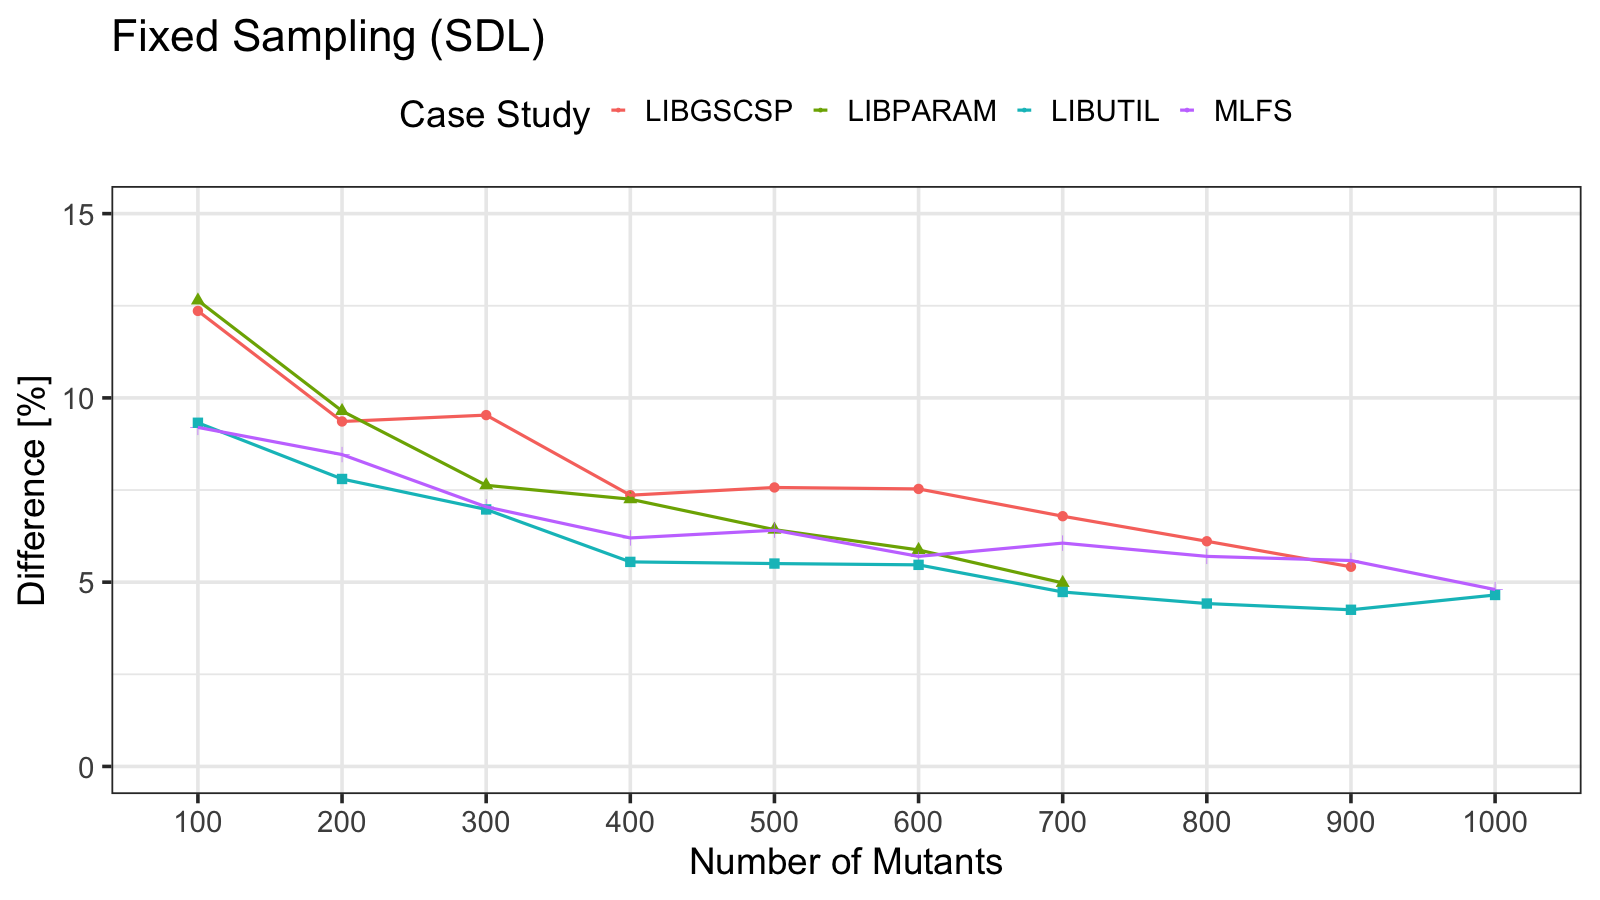
\includegraphics[width=6cm]{images/sampling_fixed_sdl}
%\caption{}
%\label{fig:results:fixedNumberOfMutantsSDL}
%\end{subfigure}
%\begin{subfigure}{.33\textwidth}
%  \centering
%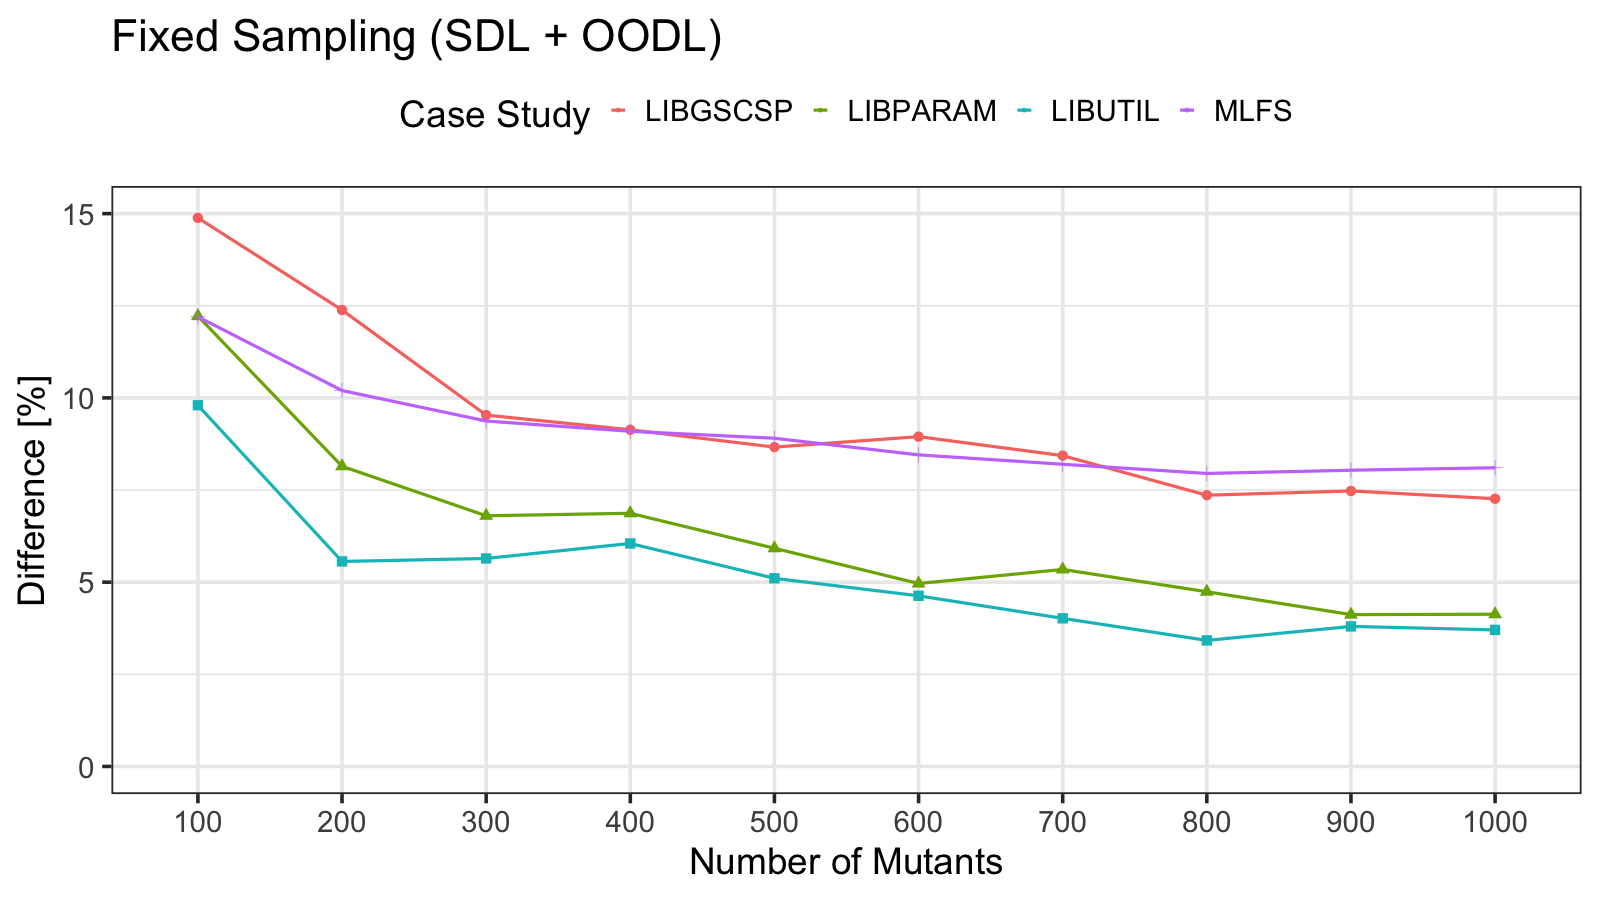
\includegraphics[width=6cm]{images/sampling_fixed_sdl_oodl}
%\caption{}
%\label{fig:results:fixedNumberOfMutantsSDLOODL}
%\end{subfigure}
%\begin{subfigure}{.33\textwidth}
%  \centering
%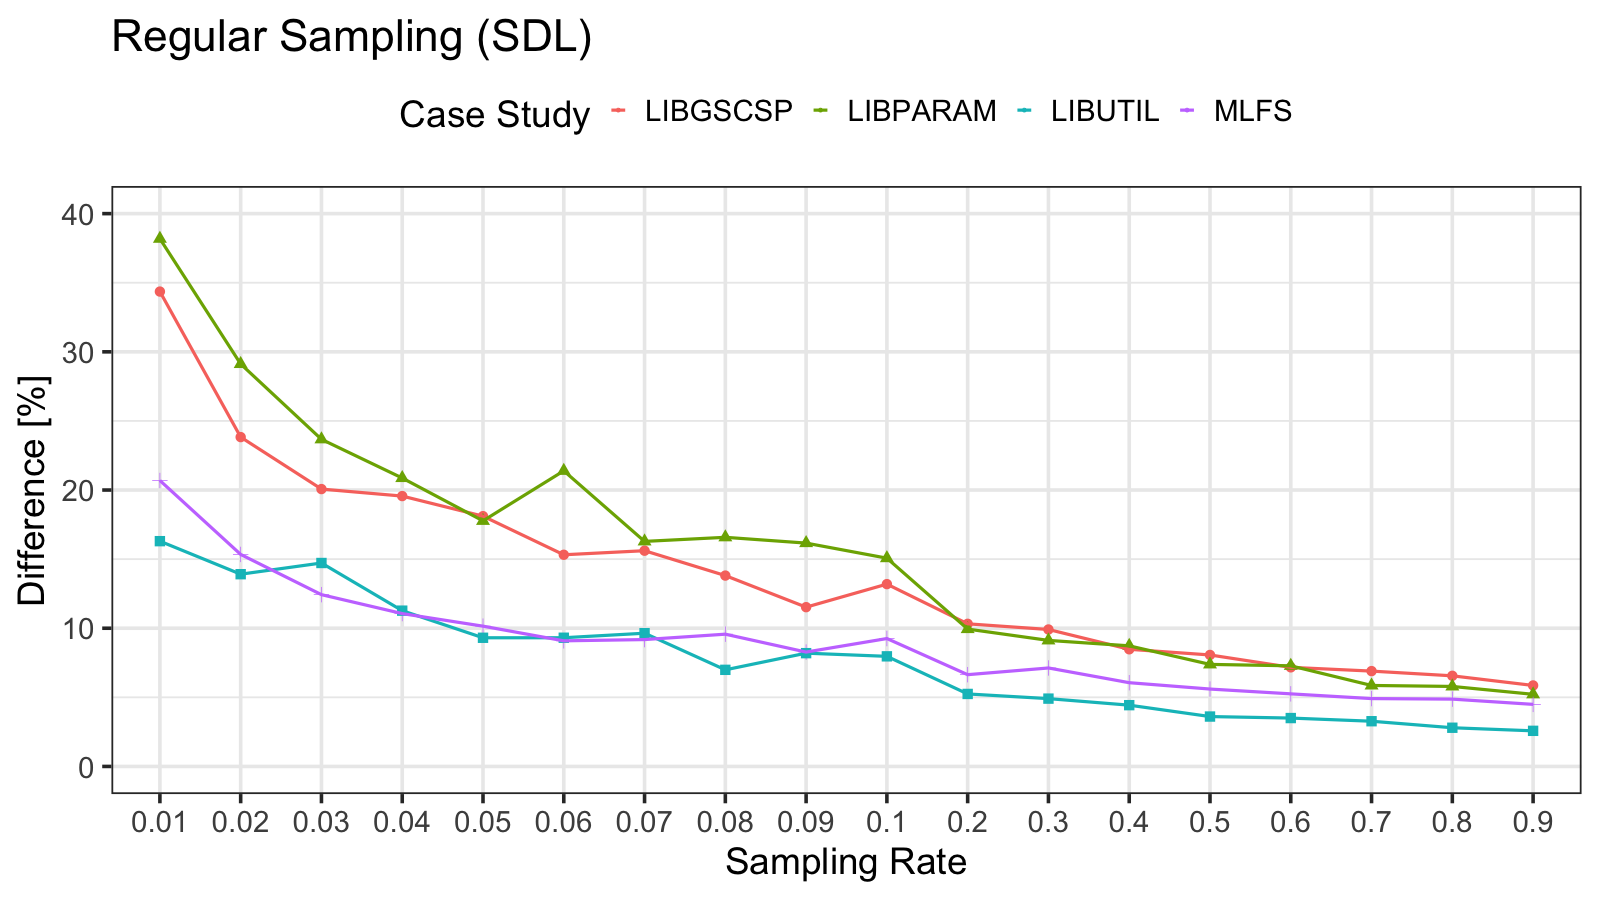
\includegraphics[width=6cm]{images/sampling_reg_sdl}
%\caption{}
%\label{fig:results:regNumberOfMutantsSDL}
%\end{subfigure}
%\begin{subfigure}{.33\textwidth}
%  \centering
%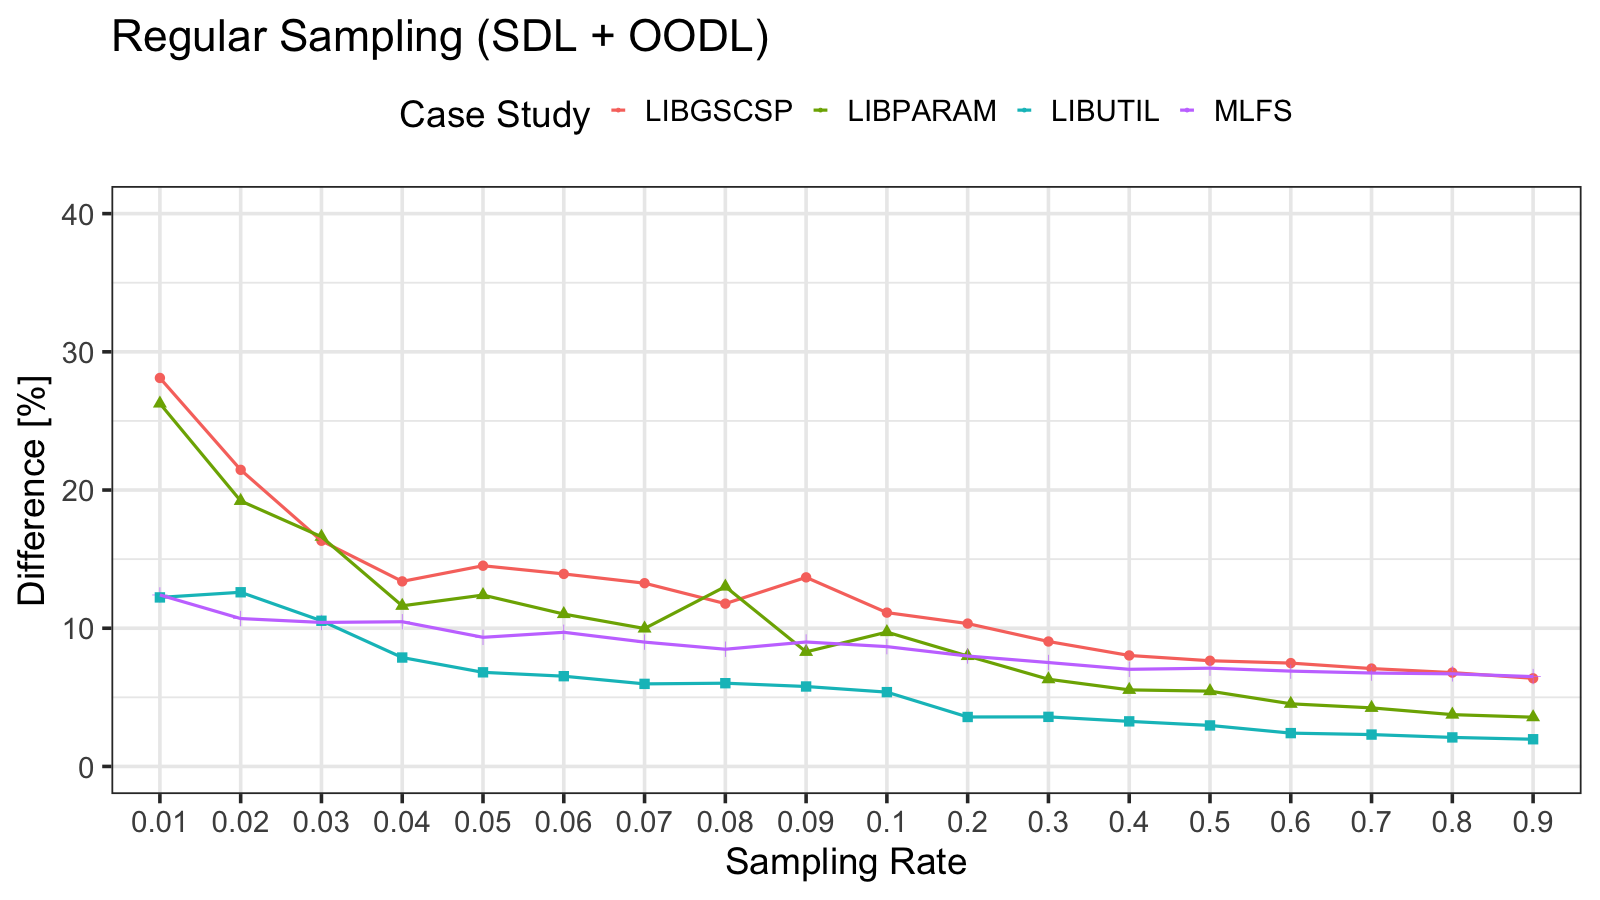
\includegraphics[width=6cm]{images/sampling_reg_sdl_oodl}
%\caption{}
%\label{fig:results:regNumberOfMutantsSDLOODL}
%
%\end{subfigure}
%\begin{subfigure}{.33\textwidth}
%  \centering
%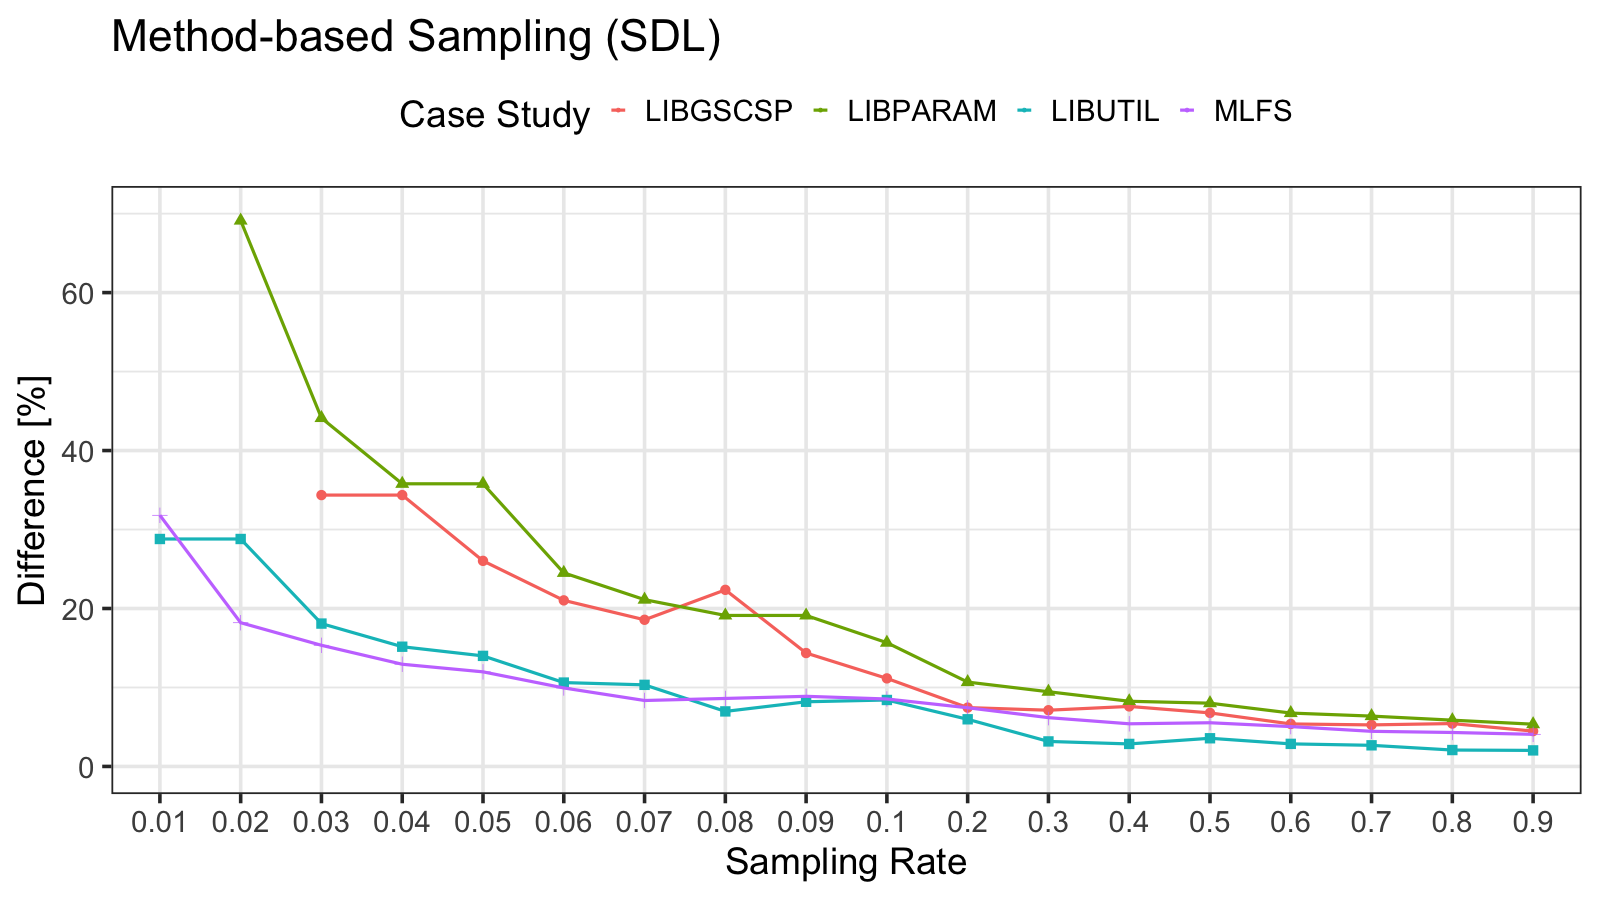
\includegraphics[width=6cm]{images/sampling_func_sdl}
%\caption{}
%\label{fig:results:funcNumberOfMutantsSDL}
%
%\end{subfigure}
%\begin{subfigure}{.33\textwidth}
%  \centering
%\includegraphics[width=6cm]{images/sampling_func_sdl_oodl}
%\caption{}
%\label{fig:results:funcNumberOfMutantsSDLOODL}
%
%\end{subfigure}
%\caption{}
%\label{fig:}
%\end{figure*}


\subsection{RQ4 - Mutation Score Accuracy with PrioritizeAndReduce}
\label{exp:accuracy:prioritize}

\subsubsection{Design and measurements}

RQ4 assesses whether the mutation score obtained with the reduced and prioritized test suite generated by \APPR (hereafter, the \MPTS) accurately estimates the actual mutation  score.
%speeds up the mutation testing process.
To this end, we compare the accuracy obtained with the four distance metrics (i.e., $D_J$, $D_O$, $D_E$, and $D_C$) used by the proposed \INDEX{PrioritizeAndReduce} algorithm (Figure 1.6 from D2). In addition, to determine to what extent our prioritization strategy based on code coverage contributes to the selection of test cases that kill mutants, we also compare the results obtained with a simple baseline that, for each mutant, randomly selects one test case among the ones that cover the mutant. 


For all subjects, we consider (a) the complete set of mutants, (b) the reduced subset of mutants providing accurate results (i.e., the one obtained with FSCI sampling with $T_{\mathit{CI}}=0.10$). 
Based on RQ3 results, we exclude mutants generated with the SDL and SDL+OODL operators only. 
%Since, based on related work, engineers may still be interested in evaluating the mutation score obtained with SDL operators only, we study to what extent the test suite derived by the \emph{PrioritizeAndReduce} algorithm enable us to estimate the mutation score computed with the SDL operator.
For FSCI sampling, since we evaluate the accuracy of a reduced test suite, we derive the confidence interval using Equation 1.5 from D2. 
%Details about the estimated accuracy and number of mutants \ref{appendix:FSCI:reduced}.

%To the end of this research question, we study if the proposed reduction/prioritization strategies can produce a mutation score that is \textit{representative} with respect to the true mutation score obtained with no test suite reduction/prioritization strategies.

%We consider the same set of mutants as for RQ2.
For each subject and each distance metric, and for each of the two sets of mutants considered, we generated ten different \MPTSs. In the case of FSCI, since it randomly selects mutants, we considered ten different sets of mutants derived with distinct executions of the FSCI algorithm. For each \MPTS, we computed the mutation score obtained. 
Then, to determine if the mutation score of the \MPTS is accurate, we follow the same procedure adopted for RQ2, i.e., we rely on the 2.5/97.5 percentile distance from the actual mutation score. 
%In the case of the SDL set, we rely on the 2.5/97.5 percentile distance from the mutation score obtained with all the SDL mutants.



\subsubsection{Results}

% !TEX root =  ../Main.tex

\begin{table}[]
\centering
\scriptsize
\caption{RQ4. Mutation score accuracy for the different strategies implemented by \emph{PrioritizeAndReduce}}
\label{table:results:PriritizeAndReduce} 
\begin{tabular}{|
p{15mm}@{\hspace{1pt}}|
p{15mm}@{\hspace{1pt}}|
>{\raggedleft\arraybackslash}p{15mm}@{\hspace{1pt}}|
>{\raggedleft\arraybackslash}p{15mm}@{\hspace{1pt}}|
>{\raggedleft\arraybackslash}p{15mm}@{\hspace{1pt}}|
}
\hline
           &          &\multicolumn{3}{c}{\textbf{$\delta_{acc}$}}\\
\hline
\textbf{Case Study} & \textbf{Strategy} & \textbf{ALL} & \textbf{FSCI (C=10)} & \textbf{SDL}  \\
\hline
\multirow{5}{*}{LIBUTIL}    
    & Random & 3.1400 & 5.87 & 3.5500  \\
           & $D_J$                    & 0.0300  & 2.54 & 0.0900  \\
           & $D_O$                    & 0.0300  & 2.54 & 0.0900  \\
           & $D_E$                    & 0.0199  & 2.51 & 0.0900  \\
           & $D_C$                    & 0.0199  & 2.57 & 0.0900 \\
\hline
\multirow{5}{*}{LIBGSCSP}   & Random & 7.2055 &  $>$5\% & 8.0605   \\
           & $D_J$                    & 1.3455  & 3.55 &1.5300 \\
           & $D_O$                    & 1.3100  & 3.55  &1.4200 \\
           & $D_E$                    & 0.7300  & 3.75  &0.6500 \\
           & $D_C$                    & 0.7300  & 3.75 &0.6500  \\
\hline
\multirow{5}{*}{LIBPARAM}   & Random & 7.7927 & $>$5\%  & 6.0892  \\
           & $D_J$                    & 0     &3.62& 0  \\
           & $D_O$                    & 0     &3.62& 0    \\
           & $D_E$                    & 0     &3.62& 0     \\
           & $D_C$                    & 0     &3.62& 0     \\
\hline
\multirow{5}{*}{MLFS}       & Random &  6.721  & $>$5\%   &    7.3999 \\
           & $D_J$                      &   0.3299   & 4.07&    0.2299    \\
           & $D_O$                      &   0.3299   & 4.07&     0.2299   \\
           & $D_E$                      &   0.0199   & 4.33&     0  \\
           & $D_C$                      &    0.0300  & 4.27&     0   \\
\hline
\multirow{5}{*}{ESAIL}      & Random & 38.8885      &   $>$5\%    &   39.1765\\
                                                & $D_J$      & 24.1688      &   $>$5\%     &  21.6800\\
                                                & $D_O$     & 24.3650      &  $>$5\%     &   21.7570\\
                                                & $D_E$     &  4.0800     &  4.7794     &   4.1400\\
                                                & $D_C$     &  3.9833    &   4.8825    &  4.5600\\
\hline
\end{tabular}
\end{table}


% \begin{table}[h]
% \centering
% \tiny
% \caption{RQ6. MS Comparison with respect to Random approach.}
% \label{table:results:msReducedRandomPVals} 
% \begin{tabular}{|llll|}
% \hline
% \textbf{Case Study}                & \textbf{\begin{tabular}[c]{@{}l@{}}MS Comparison\\w.r.t. Random\end{tabular}} & \textbf{ALL P-value} & \textbf{SDL P-value} \\
% \hline
% \multirow{4}{*}{LIBGSCSP} & $D_J$    & 1.47E-04     & 1.37E-04 \\
%                           & $D_O$    & 1.40E-04     & 1.19E-04  \\
%                           & $D_E$    & 5.18E-05     & 5.30E-05  \\
%                           & $D_C$    & 1.17E-04     & 1.08E-04  \\
% \hline
% \multirow{4}{*}{LIBUTIL}  & $D_J$    & 1.27E-04      & 1.23E-04 \\
%                           & $D_O$    & 1.20E-04      & 1.15E-04 \\
%                           & $D_E$    & 1.20E-04      & 1.15E-04  \\
%                           & $D_C$    & 1.31E-04      & 1.26E-04 \\
% \hline
% \multirow{4}{*}{LIBPARAM} & $D_J$    & 5.38E-05      & 4.96E-05 \\
%                           & $D_O$    & 5.38E-05      & 4.96E-05 \\
%                           & $D_E$    & 5.38E-05      & 4.96E-05 \\
%                           & $D_C$    & 5.38E-05      & 4.96E-05 \\
% \hline
% \multirow{4}{*}{MLFS}     & $D_J$    &  1.40E-04    &  5.30E-05\\
%                           & $D_O$    &  1.40E-04      & 5.30E-05 \\
%                           & $D_E$    &  1.36E-04      &5.30E-05 \\
%                           & $D_C$    &  1.48E-04      & 5.30E-05 \\
% \hline
% \multirow{4}{*}{ESAIL}    & $D_J$    &                \\
%                           & $D_O$    &                \\
%                           & $D_E$    &                \\
%                           & $D_C$    &               \\
% \hline
% \end{tabular}
% \end{table}



%\begin{table*}
%\tiny
%\centering
%\caption{RQ6. P-value comparison between test suite reduction approaches.}
%\label{table:results:pValComparisonTSredPrior} 
%\begin{tabular}{|l|l|lllll|l|lllll|}
%\hline
%           &          & ALL      &                       &                       &          &      &          & SDL      &                       &                       &                       &       \\
%\hline           
%Case Study &          & Random & $D_J$                  & $D_O$                  & $D_E$     & $D_C$ &          & Random & $D_J$                  & $D_O$                  & $D_E$                  & $D_C$  \\
%\hline
%LIBGSCSP   & Random &          &                       &                       &          &      & Random &          &                       &                       &                       &       \\
%           & $D_J$     & 1.47E-04 &                       &                       &          &      & $D_J$     & 1.37E-04 &                       &                       &                       &       \\
%           & $D_O$     & 1.40E-04 & 2.50E-01              &                       &          &      & $D_O$     & 1.18E-04 & 7.88E-02              &                       &                       &       \\
%           & $D_E$     & 5.18E-05 & 5.15E-05              & 4.81E-05              &          &      & $D_E$     & 5.30E-04 & 4.56E-04              & 3.80E-05              &                       &       \\
%           & $D_C$     & 1.17E-04 & 1.16E-04              & 1.10E-04              & 2.93E-02 &      & $D_C$     & 1.08E-04 & 9.55E-05              & 8.21E-05              & 6.71E-02              &       \\
%\hline
%LIBUTIL    & Random &          &                       &                       &          &      & Random &          &                       &                       &                       &       \\
%           & $D_J$     & 1.27E-04 &                       &                       &          &      & $D_J$     & 1.23E-04 &                       &                       &                       &       \\
%           & $D_O$     & 1.20E-04 & 8.31E-01              &                       &          &      & $D_O$     & 1.15E-04 & 8.31E-01              &                       &                       &       \\
%           & $D_E$     & 1.20E-04 & 8.38E-03              & 2.05E-03              &          &      & $D_E$     & 1.15E-04 & 8.31E-01              & \multicolumn{1}{r}{1} &                       &       \\
%           & $D_C$     & 1.31E-04 & 6.40E-03              & 2.20E-03              & 5.34E-01 &      & $D_C$     & 1.26E-04 & 6.80E-01              & 5.34E-01              & 5.34E-01              &       \\
%\hline
%LIBPARAM   & Random &          &                       &                       &          &      & Random &          &                       &                       &                       &       \\
%           & $D_J$     & 5.38E-05 &                       &                       &          &      & $D_J$     & 4.96E-05 &                       &                       &                       &       \\
%           & $D_O$     & 5.38E-05 & \multicolumn{1}{r}{1} &                       &          &      & $D_O$     & 4.96E-05 & \multicolumn{1}{r}{1} &                       &                       &       \\
%           & $D_E$     & 5.38E-05 & \multicolumn{1}{r}{1} & \multicolumn{1}{r}{1} &          &      & $D_E$     & 4.96E-05 & \multicolumn{1}{r}{1} & \multicolumn{1}{r}{1} &                       &       \\
%           & $D_C$     & 5.38E-05 & \multicolumn{1}{r}{1} & \multicolumn{1}{r}{1} &    \multicolumn{1}{r}{1}   &      & $D_C$     & 4.96E-05 & \multicolumn{1}{r}{1} & \multicolumn{1}{r}{1} & \multicolumn{1}{r}{1} &       \\
%\hline
%MLFS       & Random &          &                       &                       &          &      & Random &          &                       &                       &                       &       \\
%           & $D_J$     & 1.40E-04 &                       &                       &          &      & $D_J$     & 5.30E-05 &                       &                       &                       &       \\
%           & $D_O$     & 1.40E-04 & \multicolumn{1}{r}{1} &                       &          &      & $D_O$     & 5.30E-05 & \multicolumn{1}{r}{1} &                       &                       &       \\
%           & $D_E$     & 1.36E-04 & 1.20E-04              & 1.20E-04              &          &      & $D_E$     & 5.30E-05 & 1.31E-05              & 1.31E-05              &                       &       \\
%           & $D_C$     & 1.48E-04 & 1.31E-04              & 1.31E-04              & 1.61E-02 &      & $D_C$     & 5.30E-05 & 1.31E-05              & 1.31E-05              & \multicolumn{1}{r}{1} &       \\
%\hline
%ESAIL      & Random &          &                       &                       &          &      & Random &          &                       &                       &                       &       \\
%           & $D_J$     &          &                       &                       &          &      & $D_J$     &          &                       &                       &                       &       \\
%           & $D_O$     &          &                       &                       &          &      & $D_O$     &          &                       &                       &                       &       \\
%           & $D_E$     &          &                       &                       &          &      & $D_E$     &          &                       &                       &                       &       \\
%           & $D_C$     &          &                       &                       &          &      & $D_C$     &          &                       &                       &                       &      \\
%\hline           
%\end{tabular}
%\end{table*}




Table~\ref{table:results:PriritizeAndReduce} provides the values of $\delta_{acc}$ obtained for the different subjects and distance metrics (i.e., the random baseline and the four distance metrics supported by \APPR). Rows named \emph{ALL} report the results obtained when executing the entire set of mutants, rows named \emph{FSCI}  report the results obtained  with the FSCI strategy. 
%column \emph{SDL} reports the results for the mutants generated with the SDL operator only.



\NEWFSCI{Unsurprisingly, for all the subjects except \SAIL{}$_S$, the mutation score computed with the entire set of mutants tested with the \MPTS (i.e., row ALL) is more accurate than the mutation score computed with a subset of the mutants tested with the same test suite (i.e., row FSCI). 
%However, the distance metrics $D_E$ and $D_C$ enable the accurate estimation (i.e, $\delta_{acc}  < 5$) of the actual mutation score with FSCI.
However, the mutation score estimated with FSCI is always accurate (i.e, $\delta_{acc}  < 5$).
In the case of \SAIL{}$_S$, where each statement is covered by a large number of test cases (see Section~\ref{sec:empirical:subjects}),
%\footnote{\UPDATE{In $ESAIL_S$, each statement is covered on average by 61 test cases. In the other cases, each statement is covered by 2 test cases, on average (see Section~\ref{sec:empirical:subjects}).}}, 
test suite reduction has a higher probability of retaining a test case that does not kill a mutant.
For this reason, executing a reduced test suite with a subset of mutants selected with FSCI, which estimates the error due to test suite reduction, 
leads to a more accurate mutation score than executing a reduced test suite with the entire set of mutants without estimating such error (i.e., row ALL).
%For this reason, FSCI, which estimates the error due to test suite reduction, 
%performs better.
% than the execution of the entire set of mutants without estimating such error (i.e., row ALL).
%FSCI enables a more accurate computation of the mutation score for the \MPTS. 
%\FIXME{It happens because estimation errors due to test suite reduction are minimal
%\footnote{Figure~\ref{} shows that the number of test cases executed by FSCI with the whole test suite is similar to the one with the reduced test suite}, consequently 
%enforcing $|\mathit{CI}_E| \le T_{\mathit{CE}}$ simply augment the sample size thus improving the accuracy of the estimation.}
}

%enforcing PKErr, which is used to compute a corrected confidence interval and consequently the mutation score. The corrected confidence interval, which takes into account PKErr enable us to obtain a more accurate mutation score than the one computed with the whole test suite. Which is an additional reason for adopting FSCI.}}
 

%% Comment 25/02/2021:
%% In the case of ESAIL, the higher delta is likely due to the large number of test cases covering each mutant, which increases the likelihood of removing  test cases that kill the mutant. Consequently, the mutation score may be affected. In the case of FSCI, such error in the computation score is estimated with the initial tuning to estimate PKErr, which is used to compute a corrected confidence interval and consequently the mutation score. The corrected confidence interval, which takes into account PKErr enable us to obtain a more accurate mutation score than the one computed with the whole test suite. Which is an additional reason for adopting FSCI.
%% For reviewer: we realized with additional experiments, that the updated procedure lead to a mutation score that is more accurate than the mutation score computed with the whole set of mutants.


The only distance metric that consistently leads to inaccurate estimates of the mutation score (i.e., $\delta_{acc}  > 5$) across subjects is the random baseline.
Based on a non-parametric Mann Whitney test, the difference between the random baseline (i.e., Random) and the four distance metrics implemented by \APPR (i.e., $D_*$) is always significant with a \textit{p}-value $< 0.05$. This indicates that \textbf{the \APPR distance metrics are necessary to accurately estimate the mutation score while reducing the number of test cases to  execute}.

Among the proposed distance metrics, 
$D_J$ and $D_O$ provide inaccurate results with \SAIL{}$_S$.
%and less accurate results for other subjects than alternatives. 
We conjecture the main reason is their inability to account for the number of times a statement is exercised by a test case. 
We believe this is an important factor as system test cases that repeatedly exercise mutated statements, with different variable values, are more likely to kill mutants than test cases exercising such statements only once (e.g., because of the uncertainty regarding the 
\JMR{3.16}{incorrect intermediate state
%infected program state
propagating to the state variables verified by test oracles, see Section~1.2.1.1 from D2}). On the other hand, unit and integration test cases, which exercise much simpler scenarios in other subjects, are more likely to kill a mutant when the mutated statement is executed only once (e.g., because the oracle is closer to the mutated statement). This is why $D_J$ and $D_O$ fare similarly to the other distance metrics for these subjects. 
%Almost every system test case exercises certain components (e.g., the handler of telecommands, which is the main entry point of the system) but only the ones executing such components repeatedly (e.g., to verify multiple combination of input values for a same telecommand) carefully exercise mutated statements. Regarding the other subjects, each unit and integration test case rather tends to focus on simple test scenarios that exercise mutated statements once or a few times.
In contrast, $D_C$ and $D_E$ are distance metrics ensuring an accurate estimate of the mutation score and providing the lowest $\delta_{acc}$. The differences between $D_E$ and $D_C$ are always statistically significant, \UPDATE{except for \MLFS{}{}}. However, there are no practically significant differences between them. 
Since $D_C$ provides a normalized score, which is required by Step 8, we select $D_C$ as the preferred metric to be used in \APPR.
%the Based on $\delta_{acc}$, the metric that perform slightly better is $D_E$ (the sum of the $\delta_{acc}$ across all the case studies for all the configurations is lower than for $D_E$. \textbf{We thus select $D_E$ as the best metric to be used with \APPR}.


\subsection{RQ5 - Time Savings with PrioritizeAndReduce}

\subsubsection{Design and measurements}

RQ5 assesses to what extent  the \MPTS speeds up the mutation analysis process.


For each subject considered for RQ4, we measure the execution time taken by the \MPTS to execute on the mutants.
We compute time saving as the ratio of the difference in execution time from the original test suite over the time it requires to execute, for the set of mutants selected.
In particular, as in RQ4, we consider three scenarios (1) all the mutants are selected, (2) mutants are selected with FSCI sampling, (3) mutants are selected with FSCI sampling but we execute the entire test suite, as opposed to the \MPTS. By considering scenario (3), we can estimate both the time saved thanks to mutant sampling and the additional time saved when combining it with the \MPTS.
For the original test suite, to emulate a realistic mutation analysis process according to state-of-the-art solutions, we measure the time required to execute test cases until the mutant is killed (for live mutants it means that we execute the entire test suite). Also, we set a test case timeout equal to three times the duration of the original test case.

Since the execution time of test cases depends on multiple factors such as the underlying test harness, the development practices in place (e.g., verifying multiple scenarios in a single test case), and the type of testing conducted (e.g., unit, integration, system), we also compute 
the ratio of the number of test cases not executed by the \MPTS over the total number of test cases.

\subsubsection{Results}

Table~\ref{table:time:original} reports, for every subject, the time required to test all the mutants with the entire test suite, in seconds. It also reports  the total number of test cases executed. 
We observe that mutation analysis requires a large amount of time. It takes between 13 and 73 hours for subjects tested with unit and integration test suites (which are faster to execute). When a system test suite needs to be executed (i.e., $\mathit{\SAIL{}_S}$), traditional mutation analysis becomes infeasible as shown by the 11,000 hours required to perform mutation analysis with $\mathit{\SAIL{}_S}$.

Figures~\ref{fig:results:time:saving} and~\ref{fig:results:test:saving} provide boxplots depicting 
the saving achieved when the \MPTS is executed with all the mutants and with the FSCI-selected mutants, in terms of execution time and test cases, respectively. Each observation corresponds to the saving obtained with one of the ten executions performed on each subject, for a specific configuration (i.e., distance $D_*$ and strategy adopted for selecting mutants). In Figures~\ref{fig:results:time:saving} and~\ref{fig:results:test:saving}, horizontal dashed lines show the average across all subjects, whiskers are used to identify outliers (i.e., they are placed below/above 1.5*Inter Quartile Range of the upper quartile/lower quartile). A detailed table including min, max, mean, and median values for each subject is provided in Appendix C.
%~\ref{appendix:details:rq5}.

%Table~\ref{table:results:reduction:prioritize} reports the saving achieved when the \APPR test suite is executed with all the mutants, with the FSCI selected mutants, with the SDL mutants. For both time savings and test savings, we report the min, max, median, and mean values. Values are reported for all the case studies, for all the distance metrics, and for the three strategies considered to select mutants (i.e., selecting all the available mutants, selecting all the mutants generated with the SDL operator, and selecting mutants with the FSCI strategy).

Unsurprisingly, the smallest reduction in execution time and number of executed test cases is achieved when executing the \MPTS with all the mutants. 
Measuring such time reduction allows us to evaluate the benefits of test suite prioritization and selection when it is not combined with mutant selection.
Excluding outliers, execution time reduction goes from  \UPDATE{-0.52\%} % -0.11\% was the 1st quantile not the whisker
to 16.82\% and appears to be correlated with the reduction in number of test cases to execute, which varies from 4.80\% to 33.17\%.
The largest reductions are obtained with $D_J$ and $D_O$ (the median is 13.36 and 13.40, respectively), which do not consider differences in coverage frequency, thus removing the largest number of test cases; however, $D_J$ and $D_O$ also lead to the worst accuracy results according to RQ4. Metrics $D_C$ and $D_E$, instead, lead to limited benefits in terms of time reduction.

A negative reduction indicates that the reduced and prioritized test suite increases the execution time of the mutation analysis process. This happens when (1) test cases are sorted in such a way that test cases that kill the mutants are executed later with respect to the original test suite, (2) test cases that kill the mutants but have long execution times (e.g., because they trigger a timeout) are executed before test cases with shorter execution times that kill the mutants. Negative reduction, however, affects only a few executions, thus showing that a reduced and prioritized test suite tends overall to be beneficial to the mutation analysis process.



%With our subject artifacts, in terms of execution time, test suite prioritization is thus not always beneficial; however, it always lead to a reduction the number of test cases between 4.82 and 33.15. The distance metrics leading to the highest reduction in the number of test cases are $D_J$ and $D_O$, i.e., the ones with the lowest accuracy computed for RQ 4.

Mutant sampling alone contributes to a high reduction in execution time; indeed, in Figure~\ref{fig:results:time:saving}, the boxplot \emph{FSCI 0.1-Full TS}, depicting the time saving for FSCI mutants tested with the entire test suite, shows minimum, median, and maximum values of 65.76\%, 75.10\%, and 84.72\%. Indeed, by reducing the number of mutants to execute, FSCI sampling significantly reduced the total number of test cases to execute within a [\JMRCHANGE{49.98\%} - 80.54\%] range (as shown by the boxplot in Figure~\ref{fig:results:test:saving}).

The highest reduction in execution time is achieved when combining the \MPTS with FSCI sampling. It ranges from 72.09\% to 90.83\%. $D_C$ and $D_E$, which are the approaches that guarantee accurate results, lead to an execution time reduction in the ranges \JMRCHANGE{[75.25\% - 90.83\%]} and \JMRCHANGE{[73.53\% - 90.83\%]}, respectively, an impressive achievement. 
Test case savings, 
%show similar ranges, 
\JMRCHANGE{as well, are above 65\%, [68.28\% - 83.45\%]} and \JMRCHANGE{[68.08\% - 82.70\%]} for $D_C$ and $D_E$, respectively. Based on savings results, there is no practical difference between $D_C$ and $D_E$.

%The number of test cases being executed is reduced by 84.50\% for $D_J$ and $D_O$ and by 84.08\% for $D_E$ and $D_C$. When combined with FSCI sampling the differences between the different distance metrics are thus not practically significant (27 minutes, in total, across all the case studies), the selection of the coverage distance metric $D_*$ can thus rely on RQ4 results.

To conclude, \textbf{we suggest to combine FSCI sampling with the \MPTS to minimize the time required by mutation analysis}. 
For $\mathit{\SAIL{}}_S$, 
\NEWFSCI{on average, when combining the \MPTS with FSCI sampling, mutation analysis time goes from 11,000 hours to 1,531 hours, which makes mutation analysis feasible in one week with 10 computing nodes.} Note that for safety or mission critical systems, such as satellites software, the cost of using computing nodes is minimal compared to the development cost of the entire system. Indeed, to test such systems, even paying for the computational power of 100 HPC nodes to make mutation analysis feasible in half a day, is economically justifiable. \JMR{2.2}{Otherwise, without \APPR, mutation analysis leads to 11,000 hours of test cases execution, thus being practically infeasible since it would require more than 100 days to be completed, even with 100 HPC nodes.}

Our results also show that when it is not feasible to collect coverage data for the mutants under test (a requirement to generate the \MPTS), \textbf{FSCI sampling alone, without a reduced test suite, may still provide a high reduction in execution time}. In the case of $\mathit{\SAIL{}}_S$, this leads to 2,920 mutation analysis hours, which require less than two days with 100 HPC nodes.

% !TEX root =  ../Main.tex

\begin{table}[tb]
\caption{Execution time and number of test cases executed when mutation testing is based on the original test suite.}
\label{table:time:original} 
\scriptsize
\begin{tabular}{|
p{12mm}@{\hspace{2pt}}|
>{\raggedleft\arraybackslash}p{44mm}@{\hspace{1pt}}|
>{\raggedleft\arraybackslash}p{12mm}@{\hspace{1pt}}|
}
\hline
\textbf{Component}&\multicolumn{1}{c|}{\textbf{Execution time}}&\multicolumn{1}{c|}{\textbf{\# Test cases}}\\
\hline
\multirow{1}{*}{ESAIL$_S$}& 39\,604\,457 seconds (~ 11\,000 hours) & 155\,751 \\
%& SDL& & \\
\hline
\multirow{1}{*}{LIBGSCSP}&  252776 seconds (~70 hours)& 10250\\
%& SDL& 53074& 2103\\
\hline
\multirow{1}{*}{LIBPARAM}&  47949 seconds (~13 hours)& 6629\\
%& SDL& 7321& 1269\\
\hline
\multirow{1}{*}{LIBUTIL}&  214016 seconds (~59 hours)& 17672\\
%& SDL& 37603& 3030\\
\hline
\multirow{1}{*}{MLFS}&  171790 seconds (~48 hours)& 28159\\
%& SDL& 13492& 2220\\
%MLFS$_V$& 31526 &T &28069&89.03\% &X\\
\hline
\textbf{Total}&   & \\ 
\hline
\end{tabular}
\end{table}

\begin{figure}[tb]
\begin{center}
\includegraphics[width=0.8\columnwidth]{images/times.pdf}
\caption{Time savings for different sets of mutants, with the \MPTS being generated based on different distance measures.}
\label{fig:results:time:saving}
\end{center}
\end{figure}

\begin{figure}[tb]
\begin{center}
\includegraphics[width=0.8\columnwidth]{images/tests.pdf}
\caption{Test case savings for different sets of mutants, with the \MPTS being generated based on different distance measures.}
\label{fig:results:test:saving}
\end{center}
\end{figure}




\subsection{RQ6 - Precise Detection of Equivalent and Duplicate Mutants}
\label{sec:empirical:thrshold}
\subsubsection{Design and measurements}
RQ6 investigates if it is possible to identify thresholds that enable the accurate identification of mutants that are nonequivalent ($T_E$) and nonduplicate ($T_D$), following the procedure described in Section 1.2.3.7 from D2.

To determine $T_E$ and $T_D$, 
we rely on the optimal distance metric identified in RQ4 ($D_C$).
%for each normalized distance metric ($D_J$, $D_O$, $D_E$, $D_C$), 
We analyze  precision and recall of the results obtained for  different values of $T_E$ and $T_D$.
%being equal to $0.0$, between $0.0$ and $0.4$,  between $0.4$ and $0.8$, between $0.8$ and $1$.
%\CHANGED{We do not discuss recall (i.e., the percentage of equivalent mutants detected by our approach) since it is not feasible to compute the overall number of equivalent, live mutants. Indeed, it would imply manually inspecting all the live mutants, 12,330 in total, across all subjects (see Table~\ref{table:results:accuracy:full}).}
%being equal to $0.0$, $0.4$, and $0.8$.
To determine $T_E$, we measure
precision as the percentage of mutants with a distance above $T_E$ that are nonequivalent, recall as the percentage of nonequivalent mutants with a distance above $T_E$.
To determine $T_D$, we measure
precision as the percentage of mutant pairs with a distance above $T_D$ that are duplicate, recall as the percentage of duplicate mutant pairs that have a distance above $T_D$.
%\CHANGED{We do not discuss recall (i.e., the percentage of equivalent mutants detected by our approach) since it is not feasible to compute the overall number of equivalent, live mutants. Indeed, it would imply manually inspecting all the live mutants, 12,330 in total, across all subjects (see Table~\ref{table:results:accuracy:full}).}

Since the quality of results might be affected by both test suite reduction (i.e., less coverage data may be available) and mutants sampling (e.g., less mutants might be sampled), consistent with the finding of previous RQs, we consider the following two configurations: 
\begin{itemize}
\item Execution of the original test suite with all the generated mutants (ALL)
%\item Execution of the original test suite against a random selection of x\% mutants
%\item Execution of the original test suite against a random selection of x\% SDL mutants
%the following might become model-based
%\item Execution of the \APPR test suite with a random selection of x\% mutants
\item Execution of the \MPTS with FSCI sampling (\APPR)
\end{itemize}

\begin{figure}[tb]
\begin{center}
\includegraphics[width=0.6\columnwidth]{data/distanceFequency_Equivalent.pdf}
\caption{Cumulative distribution of mutants over distance values computed to determine equivalent mutants.}
\label{fig:results:test:dde}
\end{center}
\end{figure}

\begin{figure}[tb]
\begin{center}
\includegraphics[width=0.6\columnwidth]{data/distanceFequency_Redundant.pdf}
\caption{Cumulative distribution of mutant pairs over distance values computed to determine duplicate mutants.}
\label{fig:results:test:ddd}
\end{center}
\end{figure}



We determine the values of $T_E$ and $T_D$ based on the analysis of the 
cumulative distribution of the distance values computed to determine equivalent and duplicate mutants, for the two configurations listed above.
Figures~\ref{fig:results:test:dde} and
~\ref{fig:results:test:ddd}
show the cumulative distribution --- the Y-axis shows the percentage of mutants and mutant pairs with a distance lower or equal to the value in the X-axis.
For both Figures~\ref{fig:results:test:dde} and
~\ref{fig:results:test:ddd} we can observe that the distribution of mutants is not uniform in the range 0-1 (otherwise we would have straight lines with 45 degree angle) but we observe a large proportion of mutants (Figures~\ref{fig:results:test:dde}) and mutant pairs (Figures~\ref{fig:results:test:ddd}) having small distances. For example,
Figure~\ref{fig:results:test:dde} shows that, across all subjects, more than 60\% of the mutants have a distance below 0.05 (i.e., with $x$ equal to $0.05$, the value of $y$ is above $60$). 
%Also, for \PARAM{}, \UTIL{}, and \MLFS{}{} more than half of the mutants have a distance equal to zero (i.e., all the test cases show the same coverage of the original program). 
%This observation, i.e., a large percentage of mutants with a small distance from the original program, should be expected since mutation operators introduce small changes into the source code which unlikely lead to big changes to the program behaviour.
%Figure~\ref{fig:results:test:ddd} shows a similar distribution for the distances computed for duplicate mutants.

To evaluate precision and recall, we thus select values for $T_D$ and $T_E$ that 
either largely differ (i.e., $0.0$, $0.4$, and $0.8$) or delimit ranges including a large proportion of the mutants (i.e., $0$, $0.01$, and $0.05$). Table~\ref{table:results:proportion:mutants} reports the percentage of mutants and mutant pairs belonging to the ranges delimited by the selected values, for the two configurations considered in our study; the distribution of mutants in Table~\ref{table:results:proportion:mutants} is consistent with Figures~\ref{fig:results:test:dde} and
~\ref{fig:results:test:ddd}.

% !TEX root =  ../Main.tex

% \begin{table}[h]
% \caption{RQ7. Precision of Coverage-Based Detection of Equivalent Mutants.}
% \label{table:results:precision:equivalent} 
% \tiny
% \begin{tabular}{|
% p{10mm}|p{10mm}|p{10mm}|
% p{3mm}|p{3mm}|p{3mm}|p{3mm}|p{3mm}|p{3mm}|p{3mm}|p{3mm}|p{3mm}|p{3mm}|
% p{3mm}|p{3mm}|p{3mm}|p{3mm}|p{3mm}|p{3mm}|p{3mm}|p{3mm}|p{3mm}|p{3mm}|
% |}
% \hline
% \textbf{Case Study}&\textbf{Operators}&\textbf{Sampling}&\multicolumn{9}{c|}{\textbf{Precision of equivalent mutants detection when distance $< T_E$.}}&\multicolumn{9}{c|}{\textbf{Precision of redundant mutants detection when distance $< T_R$.}}\\ 
% &&
% &\textbf{0.0}&\textbf{0.0}&\textbf{0.30}&\textbf{0.40}&\textbf{0.50}&\textbf{0.60}&\textbf{0.70}&\textbf{0.80}&\textbf{0.90}
% &\textbf{0.10}&\textbf{020}&\textbf{0.30}&\textbf{0.40}&\textbf{0.50}&\textbf{0.60}&\textbf{0.70}&\textbf{0.80}&\textbf{0.90}\\
% \hline
% \\
% $\mathit{\SAIL{}}_{S}$
% &All
% &None
% &0.01
% \\
% ..
% \\
% $\mathit{\SAIL{}}_{S}$
% &All
% &\FIXME{Random 1\%}
% &0.01
% \\
% ..
% \\
% $\mathit{\SAIL{}}_{S}$
% &SDL
% &\FIXME{Random 1\%}
% &0.01
% \\
% ..
% \\

% \end{tabular}

% \end{table}
% $(0-0.40]$,  $(0.40-0.80]$, and $(0.80-1.0]$



\begin{table}[h]
\caption{Distribution (\%) of mutants in distance ranges.}
\label{table:results:proportion:mutants} 
\scriptsize
\centering
\begin{tabular}{|
@{\hspace{1pt}}p{14mm}@{\hspace{1pt}}|
@{\hspace{1pt}}p{5mm}@{\hspace{1pt}}|
@{\hspace{1pt}}>{\raggedleft\arraybackslash}p{5mm}@{\hspace{1pt}}|
@{\hspace{1pt}}>{\raggedleft\arraybackslash}p{5mm}@{\hspace{1pt}}|
@{\hspace{1pt}}>{\raggedleft\arraybackslash}p{5mm}@{\hspace{1pt}}|
@{\hspace{1pt}}>{\raggedleft\arraybackslash}p{5mm}@{\hspace{1pt}}|
@{\hspace{1pt}}>{\raggedleft\arraybackslash}p{5mm}@{\hspace{1pt}}|
>{\raggedleft\arraybackslash}p{5mm}@{\hspace{1pt}}|
@{\hspace{1pt}}>{\raggedleft\arraybackslash}p{5mm}@{\hspace{1pt}}|
@{\hspace{1pt}}>{\raggedleft\arraybackslash}p{5mm}@{\hspace{1pt}}|
@{\hspace{1pt}}>{\raggedleft\arraybackslash}p{5mm}@{\hspace{1pt}}|
@{\hspace{1pt}}>{\raggedleft\arraybackslash}p{5mm}@{\hspace{1pt}}|
@{\hspace{1pt}}>{\raggedleft\arraybackslash}p{5mm}@{\hspace{1pt}}|
}
\hline
& \multicolumn{6}{c|}{\textbf{Distance for nonequivalent}}  & \multicolumn{6}{c|}{\textbf{Distance for nonduplicate}}  \\
\cline{2-13}
\textbf{}& (0.00 & (0.00 & (0.01& (0.05 & (0.4 & (0.8
& (0.00 & (0.00 & (0.01& (0.05 & (0.4 & (0.8\\
\textbf{Config.}& 0.00] & 0.01] & 0.05]& 0.40] & 0.8] & 1.0] 
& 0.00] & 0.01] & 0.05]& 0.40] & 0.8] & 1.0] \\
\hline
ALL   
& 53.9  & 29.8  & 10.1 & 5.5  & 0.5  & 0.2  
& 39.2  & 40.5  & 7.3 & 7.6  & 2.6  & 2.8  
\\
\APPR  
% & 25.3  & 47.7  &18.0  & 8.4 & 0.6  & 0.0 
% & 36.9  & 40.2  & 7.4 & 9.5  & 3.5  & 2.5 
& 39.7  & 36.7  & 16.4  & 6.6 & 0.4  & 0.1 
& 33.7  & 37.9  & 10.5 & 10.5  & 3.8  & 3.3 
\\
\hline
\end{tabular}
\end{table}




%\begin{table}[h]
%\caption{RQ7. Precision of Coverage-Based Detection of Nonequivalent/Nonduplicate Mutants (all mutants tested with the whole test suite).}
%\label{table:results:precision:equivalent} 
%\scriptsize
%\centering
%\begin{tabular}{|
%@{\hspace{1pt}}p{12mm}@{\hspace{1pt}}|
%@{\hspace{1pt}}p{5mm}@{\hspace{1pt}}|
%@{\hspace{1pt}}>{\raggedleft\arraybackslash}p{9mm}@{\hspace{1pt}}|
%@{\hspace{1pt}}>{\raggedleft\arraybackslash}p{9mm}@{\hspace{1pt}}|
%@{\hspace{1pt}}>{\raggedleft\arraybackslash}p{10mm}@{\hspace{1pt}}|
%>{\raggedleft\arraybackslash}p{5mm}@{\hspace{1pt}}|
%@{\hspace{1pt}}>{\raggedleft\arraybackslash}p{10mm}@{\hspace{1pt}}|
%@{\hspace{1pt}}>{\raggedleft\arraybackslash}p{10mm}@{\hspace{1pt}}|
%@{\hspace{1pt}}>{\raggedleft\arraybackslash}p{10mm}@{\hspace{1pt}}|
%}
%\hline
%& \multicolumn{4}{c|}{\textbf{Nonequivalent mutants ratio}}  & \multicolumn{4}{c|}{\textbf{Nonduplicate mutants ratio}}  \\
%\textbf{Distance} & 0.0 & 0-0.4 & 0.4-0.8 & 0.8-1.0 & 0.0 & 0-0.4 & 0.4-0.8 & 0.8-1.0 \\
%  \cline{0-0}
%  \textbf{Subject} &&&&&&&&\\
%\hline
%\PARAM{}   & 0.75 & 1& 1 & 1& 0.75& 1 & 1 & 1\\
%\GCSP{}   & 0.25 & 1& 1 & 1& 1   & 1& 1 & 1\\
%\UTIL{}    & 0.25 & 1& 1 & 1& 1   & 1& 1 & 1\\
%\MLFS{}{}	   & 0.25 & 1& 1 & -& 1   & 1& 1 & 1\\
%\SAIL{}$_S$  & 0.5  & 1& 1 & -& 1   & 1& 1 & 1\\
%\hline
%\textbf{Overall}      & 0.4 & 1& 1 & 1& 0.95& 1& 1 & 1 \\
%\hline
%\end{tabular}
%\end{table}
%
%\begin{table}[h]
%\caption{RQ7. RQ7. Precision of Coverage-Based Detection of Nonequivalent/Nonduplicate Mutants (mutants sampled with FSCI, tested with \APPR test suite).}
%\label{table:results:precision:equivalent:reduced} 
%\scriptsize
%\centering
%\begin{tabular}{|
%@{\hspace{1pt}}p{12mm}@{\hspace{1pt}}|
%@{\hspace{1pt}}p{5mm}@{\hspace{1pt}}|
%@{\hspace{1pt}}>{\raggedleft\arraybackslash}p{9mm}@{\hspace{1pt}}|
%@{\hspace{1pt}}>{\raggedleft\arraybackslash}p{9mm}@{\hspace{1pt}}|
%@{\hspace{1pt}}>{\raggedleft\arraybackslash}p{10mm}@{\hspace{1pt}}|
%>{\raggedleft\arraybackslash}p{5mm}@{\hspace{1pt}}|
%@{\hspace{1pt}}>{\raggedleft\arraybackslash}p{10mm}@{\hspace{1pt}}|
%@{\hspace{1pt}}>{\raggedleft\arraybackslash}p{10mm}@{\hspace{1pt}}|
%@{\hspace{1pt}}>{\raggedleft\arraybackslash}p{10mm}@{\hspace{1pt}}|
%}
%\hline
%& \multicolumn{4}{c|}{\textbf{Nonequivalent mutants ratio}}  & \multicolumn{4}{c|}{\textbf{Nonduplicate mutants ratio}}  \\
%\textbf{Distance} & 0.0 & 0-0.4 & 0.4-0.8 & 0.8-1.0 & 0.0 & 0-0.4 & 0.4-0.8 & 0.8-1.0 \\
%  \cline{0-0}
%  \textbf{Subject} &&&&&&&&\\
%\hline
%\PARAM{}   & 0.5  & 1   & 1 & -& 1   & 1 & 1 & 1\\
%\GCSP{}   & 0.0  & 0.75& - & -& 1   & 1& 1 & 1\\
%\UTIL{}    & 0.5   & 1   & 1 & -& 1   & 1& 1 & 1\\
%\MLFS{}{}	   & 0.0   & 1   & - & -& 1   & 1& 1 & -\\
%\SAIL{}$_S$  & 0.75     & 1   & 1 & -& 1   & 1& 1 & 1\\
%\hline
%Total      & 0.35   & 0.95& 1 & -& 1   & 1& 1 & 1 \\
%\hline
%\end{tabular}
%\end{table}
%



%, $0.4$,  and $0.8$.

%Indeed, in case the distance for mutants and mutant pairs is not uniformly distributed in the range [0;1], we would like to study values for $T_E$ and $T_D$ ha.





%To determine $T_E$, for each configuration listed above (i.e., ALL and FSCI/SMTS), we manually inspect a randomly selected subset of the mutants. However, 
To compute precision and recall for different values of $T_E$, since the distribution of mutants is not uniform, we rely on stratified sampling, as follows. 
%More precisely, we estimate precision and recall based on the number of nonequivalent mutants estimated for sets of mutants selected based on their distance, 
We divide all the live mutants into six buckets, based on their distance from the original program, according to the ranges reported in Table~\ref{table:results:proportion:mutants}. 
%More precisely, we considered mutants with a distance of 0 (i.e., having the same coverage as the original program), and within the ranges $(0-0.01]$, $(0.01-0.05]$, $(0.05-0.40]$,  $(0.40-0.80]$, and $(0.80-1.0]$.  
We determine the ratio ($r_R$) of nonequivalent mutants in a specific range $R$ by randomly selecting 20 mutants (four for each subject) and inspecting them with the help of the engineers who developed the software. 
We rely on $r_R$ to estimate $e_{R}$, that is, the number of nonequivalent mutants in the entire set of mutants with a distance within the specific  range $R$
$$e_R = r_R * n_R$$
with $n_R$ being the number of mutants observed in the range $R$ for all the subjects\footnote{$n_R$ can be derived from Table~\ref{table:results:proportion:mutants}}.
Based on $e_R$, we estimate the number of nonequivalent mutants above a threshold and, consequently, compute precision and recall. We perform the analysis for both selected configurations,  ALL and \APPR.

%Our aim is to identify a threshold value above which  we observe a high precision and recall; 
Our aim is to identify a threshold value above which  we
maximize the number of nonequivalent mutants being selected (high recall) and maximize the number of equivalent mutants being discarded (high precision); since both precision and recall are equally important, we look for a threshold value that maximizes the harmonic mean of precision and recall (F-value).
%90\% of the mutants are nonequivalent. 
%Note: In case a mutant is shared by multiple configurations we may assume it is resampled
%In total, we therefore manually inspected 240 mutants (20 mutants x 6 buckets x 2 configurations)
%In total, we manually inspected 240 mutants (20 mutants x 6 buckets x 2 configurations), a larger number than that considered in related studies~\cite{schuler2013covering}.

To determine $T_D$, we repeated the same procedure as for $T_E$, except that we considered both killed and live mutants according to the procedure indicated in Section 1.2.3.7 from D2.

In total, we manually inspected 410 mutants (186 mutants to detect equivalent mutants and 224 mutant pairs to detect duplicate ones), a larger number than that considered in related studies~\cite{schuler2013covering}. The number of inspected mutants is lower than the maximum of 480 (\{20 mutants + 20 mutant pairs\} x 6 buckets x 2 configurations) because the mutant distribution across ranges is not perfectly uniform (see Table~\ref{table:results:ratio:equivalent} for the number of observations per bucket).

%duplicate
%               [,1]         [,2]        [,3]        [,4]         [,5]
%  [1,] 36.496664796 59.844728918 56.30110509 36.88708075 39.133748088
%  [2,] 48.377106531 21.876953376 20.26347083 43.87784519 38.779706252
%  [3,]  2.501076925  3.528421173  2.43483919  2.17803086  4.725099324
%  [4,]  1.225083870  1.195644418  1.67758329  1.33416054  2.223305809
%  [5,]  0.633101414  0.625080276  1.17171310  1.34543443  1.680639400
%  [6,]  0.719581761  0.551726106  1.43394443  1.09352273  1.063168534
%  [7,]  0.351142846  0.663327197  1.18294605  0.27075425  0.919557014
%  [8,]  0.687600350  0.300837722  0.96874528  0.45398330  0.804628685
%  [9,]  0.164802172  0.250317535  0.53298421  0.32920228  0.754954614
% [10,]  0.229417677  0.338228368  0.54654122  0.44697948  0.515221811
% [11,]  0.244103019  0.576558063  0.41716860  0.13338894  0.572327436
% [12,]  0.136736852  0.341368041  0.26184399  0.14314911  0.591786373
% [13,]  0.065268187  0.291704129  0.31917078  0.10236878  0.317405579
% [14,]  0.175897764  0.475232264  0.19560830  0.30028327  0.397164406
% [15,]  0.069836960  0.413865936  0.18747410  0.18478797  0.326955778
% [16,]  0.201026016  0.470665468  0.24635026  0.12335766  0.303226957
% [17,]  0.058741368  0.241754792  0.28857066  0.26521897  0.214504633
% [18,]  0.425548579  0.292274978  0.25603384  0.14945255  0.295567241
% [19,]  0.093333507  0.331378174  0.29438081  0.19095585  0.383865836
% [20,]  0.067878914  0.269726420  0.17159303  0.15175703  0.260071793
% [21,]  2.014828932  0.206362118  0.24635026  0.11615050  0.404661149
% [22,]  0.143916352  0.168971472  0.22814513  0.52813345  0.149217780
% [23,]  0.158928035  0.178105065  0.12549919  0.05575947  0.245925765
% [24,]  0.258788361  0.167829773  0.12782325  0.05381647  0.188168249
% [25,]  0.357669665  0.251744659  0.15881070  0.10058394  0.228357310
% [26,]  0.077016461  0.122447232  0.14254229  0.07618352  0.212027449
% [27,]  0.017948751  0.129297427  0.20994000  0.08169621  0.125684526
% [28,]  0.049277481  0.256026031  0.13518277  0.23986965  0.164602400
% [29,]  0.062983800  0.228339827  0.29089472  0.16522245  0.212842312
% [30,]  0.025780934  0.158981604  0.19870705  0.10410844  0.170143471
% [31,]  0.037855548  0.251744659  0.30522642  0.04862009  0.187353386
% [32,]  0.015011683  0.112171940  0.15106384  0.04416927  0.194393805
% [33,]  0.035571162  0.145281215  0.12743590  0.39867569  0.135886615
% [34,]  0.031655071  0.093619329  0.07669395  0.02835419  0.202900979
% [35,]  0.010116569  0.129868276  0.11039280  0.11461418  0.141688443
% [36,]  0.019580456  0.071927045  0.10148391  0.08296142  0.148565889
% [37,]  0.035571162  0.111315666  0.08366613  0.04832638  0.203944004
% [38,]  0.017622410  0.125016055  0.04260775  0.04502781  0.098402900
% [39,]  0.060373073  0.106748869  0.03795963  0.03056830  0.048239911
% [40,]  0.029697025  0.090765081  0.08792690  0.04053180  0.069426359
% [41,]  0.187972379  0.103894621  0.09180033  0.04166145  0.088005244
% [42,]  0.077669143  0.109888542  0.06778506  0.07550573  0.069002630
% [43,]  0.183403605  0.107034294  0.06197491  0.03515467  0.077509804
% [44,]  0.206573812  0.142997817  0.06158756  0.07997914  0.064080855
% [45,]  0.351142846  0.070499922  0.22465904  0.02227668  0.112222983
% [46,]  0.440560262  0.055372408  0.05384070  0.09934132  0.078259478
% [47,]  0.497343585  0.041386594  0.07436989  0.06583594  0.119328592
% [48,]  0.080606211  0.047095089  0.04803055  0.08921967  0.130117383
% [49,]  0.081585234  0.031682151  0.07746863  0.11944907  0.075325970
% [50,]  0.058741368  0.036248947  0.06584834  0.05115050  0.076206022
% [51,]  0.014032660  0.045097116  0.05035461  0.05853841  0.102477217
% [52,]  0.011095592  0.044526266  0.03912166  0.09742092  0.073924405
% [53,]  0.021212161  0.035392673  0.35945447  0.05318387  0.051140825
% [54,]  0.006526819  0.033680124  0.05267867  0.06974452  0.038722307
% [55,]  0.010769251  0.017696337  0.15571196  0.02263816  0.110691040
% [56,]  0.002937068  0.062222603  0.02478996  0.04080292  0.046870941
% [57,]  0.014032660  0.064220576  0.05848882  0.06649113  0.047588021
% [58,]  0.025780934  0.125301480  0.03602292  0.10182655  0.030312917
% [59,]  0.002284387  0.060510054  0.06623568  0.06933785  0.034485018
% [60,]  0.002937068  0.026829930  0.03757229  0.04762600  0.022620607
% [61,]  0.037202867  0.044811691  0.10303328  0.03016163  0.050195584
% [62,]  0.011421933  0.027971629  0.24983635  0.14312652  0.015482404
% [63,]  0.017622410  0.039959470  0.04415712  0.03562913  0.015938727
% [64,]  0.009790228  0.056514107  0.07591926  0.07878171  0.027868327
% [65,]  0.003916091  0.167829773  0.05771413  0.05311609  0.019719694
% [66,]  0.025780934  0.082773187  0.04957993  0.03840806  0.019687099
% [67,]  0.003263409  0.035392673  0.05112930  0.09484532  0.019882666
% [68,]  0.008158523  0.105607170  0.04183306  0.10715849  0.009908739
% [69,]  0.041118958  0.067645674  0.07398255  0.12918665  0.015677971
% [70,]  0.011421933  0.093619329  0.05384070  0.19563260  0.006518907
% [71,]  0.003916091  0.063078877  0.05151664  0.02977755  0.007985661
% [72,]  0.012074615  0.040244894  0.05887616  0.04405631  0.029139514
% [73,]  0.026107275  0.039103195  0.03447354  0.05291275  0.009126470
% [74,]  0.004568773  0.059939205  0.06274959  0.03400243  0.019100397
% [75,]  0.005221455  0.031111301  0.12162576  0.28677267  0.018024778
% [76,]  0.020559479  0.136147622  0.02517731  0.06179179  0.016003917
% [77,]  0.002610727  0.063649727  0.01200764  0.03264685  0.035560637
% [78,]  0.014032660  0.017410912  0.11813967  0.11585679  0.019263370
% [79,]  0.006853160  0.027115354  0.11116749  0.05621133  0.012842247
% [80,]  0.017622410  0.029398753  0.06429897  0.01509211  0.028878758
% [81,]  0.016317047  0.081631488  0.08250410  0.11739311  0.047653210
% [82,]  0.007179501  0.090765081  0.12975996  0.14073166  0.008441984
% [83,]  0.022191184  0.023404832  0.42723952  0.31569168  0.031290753
% [84,]  0.012074615  0.070785346  0.48185491  0.06590372  0.041949166
% [85,]  0.115198350  0.030825877  0.29360613  0.04071255  0.019132992
% [86,]  0.041771640  0.013414965  0.11504092  0.01671880  0.019230775
% [87,]  0.028065320  0.018838036  0.13402074  0.05124087  0.017112131
% [88,]  0.029044343  0.009704443  1.06325701  0.03063608  0.018872236
% [89,]  0.051561868  0.025973655  0.29980362  0.08592110  0.024022172
% [90,]  0.029370684  0.021121434  0.21303875  0.05467501  0.014048244
% [91,]  0.023496547  0.011987841  0.10729406  0.03404762  0.004791397
% [92,]  0.044382367  0.016554637  0.12007638  0.03904067  0.003715777
% [93,]  0.029697025  0.021121434  0.04493181  0.09552311  0.014700135
% [94,]  0.027086298  0.007135620  0.21497546  0.09762426  0.002542374
% [95,]  0.020559479  0.025973655  0.22349701  0.09613312  0.003846155
% [96,]  0.055151618  0.118736710  0.09373705  0.02125999  0.002086050
% [97,]  0.031002389  0.067360249  0.13944354  0.06610705  0.004041722
% [98,]  0.228112313  0.072783320  0.12704856  0.02128259  0.045730132
% [99,]  0.066573551  0.140714418  0.16036007  0.02659194  0.013103003
%[100,]  0.014359001  0.373906466  0.03950900  0.21958115  0.013363759
%[101,]  0.162191445  0.280001713  0.17972723  3.05574546  0.009289442


%
% precision repeat the experiment 10 times for a total of 1000 mutants inspected. Finally we compute the percentage of equivalent mutants among the selected live mutants with difference above T\%, for values of T that var between 10\% and 90\%.
%
%We repeat the experiments considering two set of mutants, the complete set, and the set derived with SDL.

%schuler2013covering says: Coverage impact—the number of methods that have at least one statement that is executed at a different frequency in the mutated run than in the normal run—while leaving out the method that contains the mutation

% Oscar: We might study T as an element of experimentation, see how different thresholds impact on the correct classification of non-equivalent mutants.

%To answer this research question, for all live mutants we estimate the code coverage difference T\% with respect to the original version, those mutants with code coverage difference lower than T\% are then classified as equivalent mutants and get discarded.

%Then, for the X\% of the mutants with code coverage difference higher than T\% we try to generate inputs using the constraint solving tool KLEE. For each of these mutants, for which we are able to generate inputs, we classify them as a \textit{correct} non-equivalent, otherwise is classified as an \textit{incorrect} non-equivalent.

%To measure the \textit{effectiveness} of our approach, we estimate the precision and recall of our technique. The \textit{precision} is the percentage of mutants that are correctly classified as non-equivalent, that is, the mutant has a code coverage difference higher than T\% and is non-equivalent. The \textit{recall} is the percentage of non-equivalent mutations that are correctly classified as such.

\subsubsection{Results}


The ratio ($r_R$) of nonequivalent mutants, for the distance ranges reported in Table~\ref{table:results:ratio:equivalent}, shows
similar results for both configurations (ALL and \APPR). 
The differences in distribution between mutants (Table~\ref{table:results:proportion:mutants}) and equivalent mutants  (Table~\ref{table:results:ratio:equivalent}), for both  configurations, is indeed not statistically significant and effect size is negligible.
%The differences between the two configurations is not statistically significant and effect size is negligible.
Such similarity suggests that nonequivalent and nonduplicate mutants follow the same distribution for both configurations. This can be explained since 
FSCI sampling uniformly selects 
%the mutants selected for \APPR using FSCI sampling are 
a subset of the mutants considered by the ALL configuration, which includes all mutants. 



The 14 nonequivalent mutants leading to $d=0$ across the two configurations (seven for ALL, seven for \APPR) have the following characteristics.
Four mutants (29\%) invalidate data buffers' preconditions (e.g., an array size is indicated as larger than it should be). Since such faults are typically detected through profiling (e.g., by using Valgrind~\cite{Valgrind}), not detecting such mutants cannot be considered a major weakness of the approach. Seven mutants (50\%) affect variables that are not used in the mutated source file (i.e., the one for which we collect code coverage). 
%Lightweight static analysis (e.g., searching for a keyword within the source code) should enable the identification of these mutants as nonequivalent. 
Static analysis should, in principle, enable the identification of these mutants as nonequivalent. 
Three mutants (21\%) concern the deletion of clauses that are not tested by our test suites; these cases might be detected by our approach after combining statement coverage with additional coverage measures (e.g., clause coverage) to compute distances, but this is left to future work. Based on the above, the percentage of nonequivalent mutants that
may potentially indicate limitations of the test suite, cannot easily be detected by other means, 
and are ignored with $T_E$, when set to zero, is very low 
 (i.e., three out of 160, or 1.88\%). For this reason, \textbf{we consider the proposed $T_E$ threshold precise enough to be used for test suite evaluation in a safety context}.
 
Table~\ref{table:results:precision:equivalent} provides precision and recall obtained for different $T_E$ values; more precisely, we report the results obtained when all mutants are considered nonequivalent (i.e., $d\ge0$), along with the results obtained for $T_E$ being set to $0$, $0.01$, $0.05$, $0.4$, and $0.8$. 

% !TEX root =  ../Main.tex

% \begin{table}[h]
% \caption{RQ7. Precision of Coverage-Based Detection of Equivalent Mutants.}
% \label{table:results:precision:equivalent} 
% \tiny
% \begin{tabular}{|
% p{10mm}|p{10mm}|p{10mm}|
% p{3mm}|p{3mm}|p{3mm}|p{3mm}|p{3mm}|p{3mm}|p{3mm}|p{3mm}|p{3mm}|p{3mm}|
% p{3mm}|p{3mm}|p{3mm}|p{3mm}|p{3mm}|p{3mm}|p{3mm}|p{3mm}|p{3mm}|p{3mm}|
% |}
% \hline
% \textbf{Case Study}&\textbf{Operators}&\textbf{Sampling}&\multicolumn{9}{c|}{\textbf{Precision of equivalent mutants detection when distance $< T_E$.}}&\multicolumn{9}{c|}{\textbf{Precision of redundant mutants detection when distance $< T_R$.}}\\ 
% &&
% &\textbf{0.0}&\textbf{0.0}&\textbf{0.30}&\textbf{0.40}&\textbf{0.50}&\textbf{0.60}&\textbf{0.70}&\textbf{0.80}&\textbf{0.90}
% &\textbf{0.10}&\textbf{020}&\textbf{0.30}&\textbf{0.40}&\textbf{0.50}&\textbf{0.60}&\textbf{0.70}&\textbf{0.80}&\textbf{0.90}\\
% \hline
% \\
% $\mathit{\SAIL{}}_{S}$
% &All
% &None
% &0.01
% \\
% ..
% \\
% $\mathit{\SAIL{}}_{S}$
% &All
% &\FIXME{Random 1\%}
% &0.01
% \\
% ..
% \\
% $\mathit{\SAIL{}}_{S}$
% &SDL
% &\FIXME{Random 1\%}
% &0.01
% \\
% ..
% \\

% \end{tabular}

% \end{table}
% $(0-0.40]$,  $(0.40-0.80]$, and $(0.80-1.0]$

\begin{table}[tb]
\caption{RQ6. Ratio ($r_R$) of Nonequivalent/Nonduplicate Mutants per Distance Range.}
\label{table:results:ratio:equivalent} 
\scriptsize
\centering
\begin{tabular}{|
@{\hspace{1pt}}p{10mm}@{\hspace{1pt}}|
@{\hspace{1pt}}p{5mm}@{\hspace{1pt}}|
@{\hspace{1pt}}>{\raggedleft\arraybackslash}p{5mm}@{\hspace{1pt}}|
@{\hspace{1pt}}>{\raggedleft\arraybackslash}p{5mm}@{\hspace{1pt}}|
@{\hspace{1pt}}>{\raggedleft\arraybackslash}p{5mm}@{\hspace{1pt}}|
@{\hspace{1pt}}>{\raggedleft\arraybackslash}p{5mm}@{\hspace{1pt}}|
@{\hspace{1pt}}>{\raggedleft\arraybackslash}p{5mm}@{\hspace{1pt}}|
>{\raggedleft\arraybackslash}p{5mm}@{\hspace{1pt}}|
@{\hspace{1pt}}>{\raggedleft\arraybackslash}p{5mm}@{\hspace{1pt}}|
@{\hspace{1pt}}>{\raggedleft\arraybackslash}p{5mm}@{\hspace{1pt}}|
@{\hspace{1pt}}>{\raggedleft\arraybackslash}p{5mm}@{\hspace{1pt}}|
@{\hspace{1pt}}>{\raggedleft\arraybackslash}p{5mm}@{\hspace{1pt}}|
@{\hspace{1pt}}>{\raggedleft\arraybackslash}p{4mm}@{\hspace{1pt}}|
}
\hline
& \multicolumn{6}{c|}{\textbf{Distance range (nonequivalent)}}  & \multicolumn{6}{c|}{\textbf{Distance range (nonduplicate)}}  \\
\textbf{}& (0.00 & (0.00 & (0.01& (0.05 & (0.4 & (0.8
& (0.00 & (0.00 & (0.01& (0.05 & (0.4 & (0.8\\
\textbf{Config.}& 0.00] & 0.01] & 0.05]& 0.40] & 0.8] & 1.0] 
& 0.00] & 0.01] & 0.05]& 0.40] & 0.8] & 1.0] \\
\hline
ALL   
& 0.35  & 0.85  & 1.00 & 1.00  & 1.00  & 1.00  
& 0.95  & 1.00  & 1.00 & 1.00  & 1.00  & 1.00  
\\
& (20)  & (20)  & (20) & (20)  & (18)  & (12)  
& (20)  & (20)  & (20) & (20)  & (20)  & (20)  
\\
\APPR  
& 0.35  & 0.95  & 1.00  & 1.00 & 1.00  & N/A
& 1.00  & 1.00 & 1.00 & 1.00  & 1.00  & 1.00
\\
& (20)  & (20)  & (20) & (10)  & (6)  & (0)  
& (20)  & (20)  & (20) & (20)  & (18)  & (16)  
\\
\hline
\end{tabular}

\textbf{Note}: We report the number of observations in parenthesis.
\end{table}


\begin{table}[tb]
\caption{RQ6. Precision (P), Recall (R), and their harmonic mean (F) obtained for the Coverage-Based Detection of Nonequivalent/Nonduplicate Mutants.}
\label{table:results:precision:equivalent} 
\scriptsize
\centering
\begin{tabular}{|
@{\hspace{1pt}}p{6mm}@{\hspace{1pt}}|
@{\hspace{1pt}}p{2mm}@{\hspace{1pt}}|
@{\hspace{1pt}}p{5mm}@{\hspace{1pt}}|
@{\hspace{1pt}}>{\raggedleft\arraybackslash}p{5mm}@{\hspace{1pt}}|
@{\hspace{1pt}}>{\raggedleft\arraybackslash}p{6mm}@{\hspace{1pt}}|
@{\hspace{1pt}}>{\raggedleft\arraybackslash}p{6mm}@{\hspace{1pt}}|
@{\hspace{1pt}}>{\raggedleft\arraybackslash}p{6mm}@{\hspace{1pt}}|
@{\hspace{1pt}}>{\raggedleft\arraybackslash}p{6mm}@{\hspace{1pt}}|
>{\raggedleft\arraybackslash}p{5mm}@{\hspace{1pt}}|
@{\hspace{1pt}}>{\raggedleft\arraybackslash}p{5mm}@{\hspace{1pt}}|
@{\hspace{1pt}}>{\raggedleft\arraybackslash}p{6mm}@{\hspace{1pt}}|
@{\hspace{1pt}}>{\raggedleft\arraybackslash}p{6mm}@{\hspace{1pt}}|
@{\hspace{1pt}}>{\raggedleft\arraybackslash}p{6mm}@{\hspace{1pt}}|
@{\hspace{1pt}}>{\raggedleft\arraybackslash}p{6mm}@{\hspace{1pt}}|
}
\hline
&& \multicolumn{6}{c|}{\textbf{Threshold (nonequivalent)}}  & 
\multicolumn{6}{c|}{\textbf{Threshold (nonduplicate)}}  \\
\cline{3-14}
\textbf{Conf.}&&\tiny{d $\ge$ 0}& \tiny{d\textgreater0} &\tiny{d\textgreater0.01}& \tiny{d\textgreater0.05}& \tiny{d\textgreater0.4} & \tiny{d\textgreater0.8}
&\tiny{d $\ge$ 0}& \tiny{d\textgreater0} &\tiny{d\textgreater0.01}& \tiny{d\textgreater0.05}& \tiny{d\textgreater0.4} & \tiny{d\textgreater0.8}
\\

\hline
\multirow{2}{*}{ALL}&P   
& 0.62  & 0.90  & 1.00 & 1.00  & 1.00  & 1.00  
& 0.98  & 1.00  & 1.00 & 1.00  & 1.00  & 1.00  \\
&R   
& 1.00  & 0.71  & 0.28 & 0.10  & 0.01  & 0.01
& 1.00  & 0.62  & 0.21 & 0.13  & 0.05  & 0.03  
\\
&F   
& 0.77  & \underline{0.80}  & 0.44 & 0.19  & 0.03  & 0.01
& \underline{0.99}  & 0.77  & 0.34 & 0.23  & 0.10  & 0.05  
\\
\hline
\multirow{1}{*}{\emph{MA}}&P 
& 0.81  & 0.97  & 1.00  & 1.00 & 1.00 & N/A 
& 1.00  & 1.00 & 1.00 & 1.00  & 1.00  & 1.00
\\
\multirow{1}{*}{\emph{SS}}&R
& 1.00  & 0.89  & 0.33  & 0.11 & 0.01  & N/A
& 1.00  & 0.63 & 0.22 & 0.16  & 0.06  & 0.02
\\
&F   
& 0.90  & \underline{0.93}  & 0.50 & 0.20  & 0.02  & N/A
& \underline{1.00}  & 0.77  & 0.37 & 0.27  & 0.11  & 0.05  
\\
\hline
\end{tabular}
\end{table}



%
%
%
%
%
%
%\begin{table}[h]
%\caption{RQ6. Precision (P) and Recall (R) of Coverage-Based Detection of Nonequivalent/Nonduplicate Mutants.}
%\label{table:results:precision:equivalent} 
%\scriptsize
%\centering
%\begin{tabular}{|
%@{\hspace{1pt}}p{5mm}@{\hspace{1pt}}|
%@{\hspace{1pt}}p{10mm}@{\hspace{1pt}}|
%@{\hspace{1pt}}p{5mm}@{\hspace{1pt}}|
%@{\hspace{1pt}}>{\raggedleft\arraybackslash}p{5mm}@{\hspace{1pt}}|
%@{\hspace{1pt}}>{\raggedleft\arraybackslash}p{5mm}@{\hspace{1pt}}|
%@{\hspace{1pt}}>{\raggedleft\arraybackslash}p{5mm}@{\hspace{1pt}}|
%@{\hspace{1pt}}>{\raggedleft\arraybackslash}p{5mm}@{\hspace{1pt}}|
%@{\hspace{1pt}}>{\raggedleft\arraybackslash}p{5mm}@{\hspace{1pt}}|
%>{\raggedleft\arraybackslash}p{5mm}@{\hspace{1pt}}|
%@{\hspace{1pt}}>{\raggedleft\arraybackslash}p{5mm}@{\hspace{1pt}}|
%@{\hspace{1pt}}>{\raggedleft\arraybackslash}p{5mm}@{\hspace{1pt}}|
%@{\hspace{1pt}}>{\raggedleft\arraybackslash}p{5mm}@{\hspace{1pt}}|
%@{\hspace{1pt}}>{\raggedleft\arraybackslash}p{5mm}@{\hspace{1pt}}|
%@{\hspace{1pt}}>{\raggedleft\arraybackslash}p{5mm}@{\hspace{1pt}}|
%}
%\hline
%&& \multicolumn{6}{c|}{\textbf{Nonequivalent mutants ratio}}  & \multicolumn{6}{c|}{\textbf{Nonduplicate mutants ratio}}  \\
%\cline{2-14}
%&\textbf{Distance}& 0.00 & 0.00 & 0.01& 0.05 & 0.4 & 0.8
%& 0.00 & 0.00 & 0.01& 0.05 & 0.4 & 0.8\\
%&\textbf{range}& 0.00 & 0.01 & 0.05& 0.40 & 0.8 & 1.0 
%& 0.00 & 0.01 & 0.05& 0.40 & 0.8 & 1.0 \\
%\hline
%\multirow{2}{*}{$r_R$}&ALL   
%& 0.35  & ?  & ? & 1  & 1  & 1  
%& 0.95  & ?  & ? & 1  & 1  & 1  
%\\
%&SMTS  
%& 0.35  & ?  & ?  & 0.95 & 1  & 1
%& 0.35  & ? & ? & 1  & 1  & 1
%\\
%\hline
%\multirow{2}{*}{P}&ALL   
%& 0.35  & ?  & ? & 1  & 1  & 1  
%& 0.95  & ?  & ? & 1  & 1  & 1  
%\\
%&SMTS  
%& 0.35  & ?  & ?  & 0.95 & 1  & 1
%& 0.35  & ? & ? & 1  & 1  & 1
%\\
%\hline
%\multirow{2}{*}{R}&ALL   
%& 0.35  & ?  & ? & 1  & 1  & 1  
%& 0.95  & ?  & ? & 1  & 1  & 1  
%\\
%&SMTS  
%& 0.35  & ?  & ?  & 0.95 & 1  & 1
%& 0.35  & ? & ? & 1  & 1  & 1
%\\
%\hline
%\end{tabular}
%\end{table}



%\begin{table}[h]
%\caption{RQ7. Precision of Coverage-Based Detection of Nonequivalent/Nonduplicate Mutants (all mutants tested with the whole test suite).}
%\label{table:results:precision:equivalent} 
%\scriptsize
%\centering
%\begin{tabular}{|
%@{\hspace{1pt}}p{12mm}@{\hspace{1pt}}|
%@{\hspace{1pt}}p{5mm}@{\hspace{1pt}}|
%@{\hspace{1pt}}>{\raggedleft\arraybackslash}p{9mm}@{\hspace{1pt}}|
%@{\hspace{1pt}}>{\raggedleft\arraybackslash}p{9mm}@{\hspace{1pt}}|
%@{\hspace{1pt}}>{\raggedleft\arraybackslash}p{10mm}@{\hspace{1pt}}|
%>{\raggedleft\arraybackslash}p{5mm}@{\hspace{1pt}}|
%@{\hspace{1pt}}>{\raggedleft\arraybackslash}p{10mm}@{\hspace{1pt}}|
%@{\hspace{1pt}}>{\raggedleft\arraybackslash}p{10mm}@{\hspace{1pt}}|
%@{\hspace{1pt}}>{\raggedleft\arraybackslash}p{10mm}@{\hspace{1pt}}|
%}
%\hline
%& \multicolumn{4}{c|}{\textbf{Nonequivalent mutants ratio}}  & \multicolumn{4}{c|}{\textbf{Nonduplicate mutants ratio}}  \\
%\textbf{Distance} & 0.0 & 0-0.4 & 0.4-0.8 & 0.8-1.0 & 0.0 & 0-0.4 & 0.4-0.8 & 0.8-1.0 \\
%  \cline{0-0}
%  \textbf{Subject} &&&&&&&&\\
%\hline
%\PARAM{}   & 0.75 & 1& 1 & 1& 0.75& 1 & 1 & 1\\
%\GCSP{}   & 0.25 & 1& 1 & 1& 1   & 1& 1 & 1\\
%\UTIL{}    & 0.25 & 1& 1 & 1& 1   & 1& 1 & 1\\
%\MLFS{}{}	   & 0.25 & 1& 1 & -& 1   & 1& 1 & 1\\
%\SAIL{}$_S$  & 0.5  & 1& 1 & -& 1   & 1& 1 & 1\\
%\hline
%\textbf{Overall}      & 0.4 & 1& 1 & 1& 0.95& 1& 1 & 1 \\
%\hline
%\end{tabular}
%\end{table}
%
%\begin{table}[h]
%\caption{RQ7. RQ7. Precision of Coverage-Based Detection of Nonequivalent/Nonduplicate Mutants (mutants sampled with FSCI, tested with \APPR test suite).}
%\label{table:results:precision:equivalent:reduced} 
%\scriptsize
%\centering
%\begin{tabular}{|
%@{\hspace{1pt}}p{12mm}@{\hspace{1pt}}|
%@{\hspace{1pt}}p{5mm}@{\hspace{1pt}}|
%@{\hspace{1pt}}>{\raggedleft\arraybackslash}p{9mm}@{\hspace{1pt}}|
%@{\hspace{1pt}}>{\raggedleft\arraybackslash}p{9mm}@{\hspace{1pt}}|
%@{\hspace{1pt}}>{\raggedleft\arraybackslash}p{10mm}@{\hspace{1pt}}|
%>{\raggedleft\arraybackslash}p{5mm}@{\hspace{1pt}}|
%@{\hspace{1pt}}>{\raggedleft\arraybackslash}p{10mm}@{\hspace{1pt}}|
%@{\hspace{1pt}}>{\raggedleft\arraybackslash}p{10mm}@{\hspace{1pt}}|
%@{\hspace{1pt}}>{\raggedleft\arraybackslash}p{10mm}@{\hspace{1pt}}|
%}
%\hline
%& \multicolumn{4}{c|}{\textbf{Nonequivalent mutants ratio}}  & \multicolumn{4}{c|}{\textbf{Nonduplicate mutants ratio}}  \\
%\textbf{Distance} & 0.0 & 0-0.4 & 0.4-0.8 & 0.8-1.0 & 0.0 & 0-0.4 & 0.4-0.8 & 0.8-1.0 \\
%  \cline{0-0}
%  \textbf{Subject} &&&&&&&&\\
%\hline
%\PARAM{}   & 0.5  & 1   & 1 & -& 1   & 1 & 1 & 1\\
%\GCSP{}   & 0.0  & 0.75& - & -& 1   & 1& 1 & 1\\
%\UTIL{}    & 0.5   & 1   & 1 & -& 1   & 1& 1 & 1\\
%\MLFS{}{}	   & 0.0   & 1   & - & -& 1   & 1& 1 & -\\
%\SAIL{}$_S$  & 0.75     & 1   & 1 & -& 1   & 1& 1 & 1\\
%\hline
%Total      & 0.35   & 0.95& 1 & -& 1   & 1& 1 & 1 \\
%\hline
%\end{tabular}
%\end{table}
%



 We can observe that \textbf{$T_E$ set to zero enables the accurate detection of nonequivalent mutants}. Indeed, 
for $d>0$, we achieve the highest F-value, and the highest precision and recall, given that a value of $1.00$ cannot be achieved simultaneously for precision and recall.
These results are in line with related work~\cite{zhang2013faster} reporting that a difference in the frequency of execution of a single line of code (i.e., $d>0$) is indicative of a mutant not being equivalent to the original software.
Moreover, these results also indicate that \textbf{FSCI mutants sampling and \MPTS selection enable the accurate identification of nonequivalent mutants based on $T_E$}.



As for duplicate mutants, based on Table~\ref{table:results:precision:equivalent}, 
mutants are highly likely to be nonduplicate and thus \textbf{it is not possible to determine a threshold to identify duplicate mutants}. Indeed, among all the considered threshold values, the highest F-value is obtained when all the mutants are considered nonduplicate (i.e., $d\ge0$). These results are in line with related work~\cite{shin2017theoretical} showing that test suites are unlikely to distinguish nonredundant mutants (i.e., many nonduplicate and nonsubsumed mutants yield the same test results). 
%SHin et al show that 60,043 out of 242,437 mutants are detected as nonredundant.
With test suites that do not distinguish nonredundant mutants, it is very likely that nonduplicate mutants show the same coverage in addition to showing the same results. This is the reason why in Table~\ref{table:results:ratio:equivalent}, we observe a large percentage of nonduplicate mutants having the same coverage (i.e., $d=0$). For this reason, when no methods are available to automatically generate test cases that distinguish subsumed mutants (see Section~1.2.2 from D2), we suggest that all mutants should be considered as nonduplicate when computing the mutation score:

\begin{equation}
\label{equation:ms:exp}
\mathit{MS} = \frac{\mathit{KND}}{\mathit{LNE}+\mathit{KND}}
\end{equation}

where $\mathit{LNE}$ is the number of live, nonequivalent mutants.







\subsection{RQ7 - \APPR Mutation Score}

\subsubsection{Design and measurements}

% Describe what it the purpose of the RQ
\JMR{3.16}{RQ7 investigates the extent to which  the mutation score estimated by MASS with Equation~\ref{equation:ms:exp}},
%RQ7 investigates the extent to which \APPR's mutation score estimate (i.e., the mutation score computed with Equation~\ref{equation:ms:exp}), 
%when relying on FSCI and a reduced and prioritized test suite, 
can accurately predict
the actual mutation score of the system.

% an over- or under- approximation of the mutation score computed with a  non-optimized mutation testing process (i.e., no mutants sampling and no test suite reduction/prioritization). 

To this end, we apply \APPR to the five subjects  described in Section~\ref{sec:empirical:subjects} and compute the mutation score according to equation~\ref{equation:ms:exp}.
\REVOCT{C-P-11}{We compare the resulting mutation scores with those obtained with a traditional, non-optimized mutation analysis process that tests all the mutants with the entire test suite and do not discard likely equivalent mutants.}
Since we have already demonstrated that FSCI, applied to a reduced and prioritized test suite, accurately estimates the mutation score (see RQ4), 
we discuss the percentage of live mutants that are discarded by means of $T_E$ and the effect it has on the mutation score.
\REVOCT{C-P-11}{We aim to discuss deviations between the two approaches; in particular, given that \APPR filters out equivalent mutants, we expect the \APPR mutation score to be higher than the one of the traditional approach. Unfortunately, in our context, it is still not feasible to automatically identify equivalent and redundant mutants; for this reason, comparison of the \APPR mutation score with a ground truth mutation score is not possible. A manual investigation of the equivalent and redundant mutants reported by \APPR has been performed to address RQ6.}
%If the percentage of equivalent mutant discarded matches the one observed for RQ6 (i.e., 65\%), whose correctness was manually verified, we can conclude that \APPR enables the accurate estimation of the mutation score.



% Describe what we measure (ideally the same measurement of the referred papers)

\subsubsection{Results}
From Table~\ref{table:results:mutationScore}, one can see that, on average, the percentage of live mutants that are discarded because considered equivalent is 42.28\%, which is in line with related work (i.e., 45\%~\cite{zhang2013faster}). Across our subjects, such percentage varies from 2.61\% (\SAIL{}$_S$) to 69.37\% (\MLFS{}{}), because of nondeterminism.
%based on the nondeterministic nature of the system. 
Indeed, complex embedded software, even when generating consistent functional results across multiple runs, may show nondeterminism 
in their nonfunctional properties (e.g., number of tasks started) 
%when the test environment is not well isolated (e.g., multiple test suites are run in parallel thus affecting performance).
when it is not possible to control the resources provisioned by the test environment.
For example, in our environment, \SAIL{}$_S$, which is a system including real-time tasks, show different code coverage for multiple executions of a same test case. The same happens for \GCSP{}, a network library, which may execute 
a different set of instructions
%different number of functions 
based on the current network usage (e.g., ports available on the host OS). 
%For such systems, the removal of equivalent mutants based on code coverage appears to be less effective. 
Unsurprisingly, in our experiments, the subject having the largest number of predicted equivalent mutants removed is the mathematical library \MLFS{}{}, which should not be affected by nondeterministic behaviour due to real-time constraints or networking. 

To maximize the number of equivalent mutants detected by \APPR, it is therefore advisable to minimize the sources of nondeterminism. It can be achieved, for example, by executing test cases in a dedicated testing environment, which is standard practice for space software. However, since our analysis concerned the execution of a large, entire set of mutants, not only a sampled subset, we relied on a shared HPC environment. This may have introduced unexpected delays in the execution of the simulator and altered the number of available ports, thus exacerbating nondeterminism.

As expected, the removal of equivalent mutants results in the \APPR mutation score being higher than that computed with a traditional approach. On average, the score increased by 10.52 percentage points (i.e., from $70.62\%$ to $81.14\%$). 

To provide some additional insights about the software features that, according to \APPR mutation analysis results, 
warrant to be verified with additional test cases, we report on the characteristics of
manually inspected mutants having $d > 0$ in Table~\ref{table:results:ratio:equivalent}.
%56 in total, I do want explain why, thus I do not put the number
According to our analysis, live mutants concern (1) logging functions (11\%),  (2) code developed by third parties (5\%), (3) time operations (e.g., timeouts, 4\%), (4) thread synchronisations (e.g., mutex locks, 5\%), (5) memory operations (e.g., malloc and free operations, 20\%), and (6) the application logic (55\%). Most of these categories either do not need to be tested (cases 1 and 2), or concern operations that are difficult to test (cases 3, 4, and 5) and often verified by other means, e.g., test suites including hardware in the loop or through manual inspection. However, most of the live mutants concerning the application logic have enabled engineers to identify weaknesses  in test suites
(e.g., corner cases not being tested, scenarios testable with simulators but verified only by test suites with hardware in the loop), 
which further stresses the importance of mutation analysis in this context.
Furthermore, the manual inspection of these live mutants led to the identification of 
one previously undetected bug
\JMR{3.15} {since the test suite was not covering a specific combination of boolean clauses in a function, a problem that may occur even when MC/DC adequacy is achieved by test suites~\cite{Gay2016}.}


% enable us to characterize the type of functions presenting live, nonequivalent mutants.
%based on the characteristics of the mutated source code: 
%(1) code that is executed with nondeterministic frequency (e.g., port opening closing), \FIXME{(2) functionalities writing to standard output,
%The main reasons for these mutants to not be killed are the following: 
%(1) the mutants are covered by other test suites (e.g., Unit test suite for $\SAIL{}\emph{-CSW}$ or hardware in the loop test suite for ONE case studies), 
%(2) \FIXME{return values of functions not propagated through the code, 
%(3) missing verification of corner cases and specific inputs, 
%(4) missing verification of final variables and final array’s values, 
%(5) missing verification of the negated condition on if and while closures, 
%(6) missing verification of variable values after iteration loops, and 
%(7) missing verification of time deltas between specific instructions}.
%
%These results indicate that, to be used as an acceptance criterion the mutation score should be computed by relying on all the software test suites.
 
% !TEX root =  ../Main.tex

\begin{table}[htb]
\caption{RQ7. \APPR Mutation Score.}
\label{table:results:mutationScore} 
\small
\centering
\begin{tabular}{|
>{\raggedleft\arraybackslash}p{24mm}@{\hspace{1pt}}|
>{\raggedleft\arraybackslash}p{46mm}@{\hspace{1pt}}|
>{\raggedleft\arraybackslash}p{25mm}@{\hspace{1pt}}|
>{\raggedleft\arraybackslash}p{25mm}@{\hspace{1pt}}|
}
\hline
\textbf{Subject}&\textbf{Predicted Equivalent}&\multicolumn{2}{c|}{\textbf{Mutation Score (\%)}}\\
&\textbf{Mutants Removed (\%)}&\textbf{Traditional}&\textbf{\APPR}\\ 
\hline
% 1225-32=1193; 2311/(2311+1193)
\SAIL{}$_{S}$&2.61&65.36&65.95\\
%$\mathit{\SAIL{}}$&&\\
% 4198-2281=1917; 10376/(10376+1917)


% 1214-770=444; 2717/(2717+444)

% 1712-371=1341; 3270/(3270+1341)
\GCSP{}&21.67&65.64&70.92\\
\PARAM{}&63.43&69.12&85.95\\
% 3981-2699=1282; 17484/(17484+1282)
\UTIL{}&54.34&71.20&84.41\\
\MLFS{}{}&69.37&81.80&93.49\\
\hline
$\textbf{Average}$&42.28&70.62&81.14\\
\hline
\end{tabular}

\end{table}

%2021-06-14
%Average MS with reduced test suite, above is with the whole TS
% 
%CSP 70.92
%LIBUTIL 84.41
%PARAM 85.95
%MLFS 93.49
%ESAIL 65.95





\clearpage
\subsection{RQ8 - Threshold for the mutation score}
\label{sec:exp:thr}
\subsubsection{Design and measurements}


RQ8 aims to determine if it is possible to identify a threshold for the mutation score that ensures that the fault revealing power of a test suite is greater than the one of a test suite that simply achieves statement coverage adequacy (i.e., all the statements are covered).


We may perform an experiment in line with the one performed in reference [78]. The objective of the experiment would be to identify a mutation score that ensures that the fault revealing power of a test suite is greater than the one of a test suite that simply achieves statement coverage adequacy (i.e., all the statements are covered). 

Related work~\cite{CChekam:17} identify a threshold for the mutation score that ensures that a test suite with a mutation score above the given threshold detects all the mutants detected by a test suite that achieves statements coverage adequacy. 
We may perform an experiment in line with the one performed in reference~\cite{CChekam:17}.
To replicate such study, for every case study system, we may consider the original test suite, $\mathit{TS}_o$, which achieves 100\% coverage of non dead code, and an extended test suite, $\mathit{TS}_e$, that consists of the same test cases of $\mathit{TS}_o$ plus a set of test cases automatically generated to kill the mutants. The extended test suite achieves a mutation score $ms_e$ that is greater than the mutation score $\mathit{ms}_o$ of the original test suite. For example, we may have $\mathit{ms}_o=0.7$ and $\mathit{ms}_e=0.9$.

The experiment can be conducted by dividing the interval between $m_o$ and $m_i$ into $n$ ranges (e.g., 4 ranges), such that we can define $\delta = (\mathit{ms}_e - \mathit{ms}_o)/n$ and have each of the $n$ ranges defined as the interval between $\mathit{ms}_o+(n-1)*\delta$ and $\mathit{ms}_o+n*\delta$.
For every case study, for each of the $n$ ranges, we can generate $M$ test suites  (e.g., 10) by randomly selecting test cases belonging to $\mathit{TS}_i$ till we achieve a mutation score in the given range.
For each i-th test suite belonging to the range $n$ (i.e., $\mathit{TS}_{n,i}$), we compute the mutation score (i.e., $ms_{n,i}$).
Also, we compute the \INDEX{mutation score delta} as $msd_{n,i}=ms_{n,i}-ms_o$. Each test suite in the range $n$ enable us to study the fault revealing power of a test suite with a mutation score above the threshold $T=(n-1)*\delta$.

For each range $n$ we can perform a one sample t-test to reject the null hypothesis $msd_{n} = 0$ in favor of the alternate hypothesis $msd_{n} > 0$, at a 5\% alpha level.
If the null hypothesis is rejected in favor of the alternate hypothesis then the threshold $T=(n-1)*\delta$ ensures to achieve better fault detection than statement coverage adequacy.
Alternatively, we may perform a one sample wilcoxon-signed-rank test, which evaluates whether the median of the sample is greater than zero.

\REVNOV{PTCR-7}{Unfortunately, contrary to what we wrote in the previous version of report D2, such experiment would be of little value in our context because \APPR require the test suite to achieve a maximal statements coverage. Consequently, any test suite $\mathit{TS}_e$ would have a better mutation score than $\mathit{TS}_o$. Also, based on our assumption, it makes no sense to select a test suite $\mathit{TS}_e$ that does not achieve the same statement coverage of $\mathit{TS}_o$.}

\REVNOV{PTCR-7}{For this reason, the experiment should be performed with a set of real faults affecting the case study system not mutants. 
More precisely, for each i-th test suite belonging to the range $n$ (i.e., $\mathit{TS}_{n,i}$), we should compute the fault detection rate (i.e., $fdr_{n,i}$) as the proportion of real faults detected by the test suite. Similarly to what indicated above, we may compute the \INDEX{fault detection rate delta} as $fdrd_{n,i}=fdr_{n,i}-fdr_o$. Each test suite in the range $n$ enable us to study the fault revealing power of a test suite with a mutation score above the threshold $T=(n-1)*\delta$.}

\REVNOV{PTCR-7}{For each range $n$ we can perform a one sample t-test to reject the null hypothesis $fdr_{n} = 0$ in favor of the alternate hypothesis $fdr_{n} > 0$, at a 5\% alpha level.
If the null hypothesis is rejected in favor of the alternate hypothesis then the threshold $T=(n-1)*\delta$ ensures to achieve better fault detection than statement coverage adequacy.
Alternatively, we may perform a one sample wilcoxon-signed-rank test, which evaluates whether the median of the sample is greater than zero.}

\REVNOV{PTCR-7}{Despite such experiment would be of great value, the required information is not currently available and thus it is not possible at this stage of the project to commit for addressing this research question.}
\REVOCT{C-P-12}{To address this research question, a dedicated activity, with tasks planned for this purpose, might be needed.}

\clearpage
\subsection{RQ9 - Combined mutation analysis results}
\label{sec:exp:thr}

\STARTCHANGEDWPT
\subsubsection{Design and measurements}


RQ9 aims to determine whether is possible to combine results of mutation analysis for different test suites targeting the same system.

In CPSs, it is a common practice to verify and validate a system with different types of test suites. For example, it might be common to have a unit test suite verifying isolated components of a system, and then having a system test suite verifying complex use case scenarios of certain functionalities.

To answer this research question, we verify whether the mutation analysis results of an additional test suite can further improve the existing mutation score. We say that if the additional test suite is able to kill additional mutants, with respect to the existing test suite, then we conclude that mutation results from two test suites can be actually be combined.

In our experiments, in addition to the assessment of the ESAIL$_s$ system test suite, we also analyzed the ESAIL$_s$ unit test suite with the 3\,536 mutants previously generated.

\subsubsection{Results}

The mutation score of the unit test suite is 26.78\%; there are 947 killed mutants, and 2\,589 live mutants. 

In addition to the set of 2\,311 mutants killed by the system test suite, we observe that the unit test suite kills 184 additional mutants. 
The result of mutation analysis combined for both test suites produce a mutation score of 70.56\% (an improvement of +4,8\%), which indicates that mutation analysis results can effectively be combined for different test suites (e.g., system and units).

\ENDCHANGEDWPT

\subsection{Discussion}
\label{sec:emp:discussion}

\JMR{2.3}{Our results show that the \APPR pipeline helps to overcome mutation analysis limitations caused by common  characteristics of embedded software, present in space systems and, more generally, in similar CPS (e.g., avionics, automotive, and industry 4.0).}

\JMRCHANGE{Although the need for dedicated hardware and simulators prevent the applicability of optimizations that make use of multi-threading or other OS functions to minimize mutants compilation time~\cite{untch1993mutation}, we have shown that our selective compilation strategy (see Section~1.2.7 from D2) is sufficient to achieve an efficient mutant compilation process (see Section~\ref{experimnt:setup}).}

\REVNOV{PTCR-PABG-27}{Trivial compiler optimization approaches are useful to eliminate a large proportion of mutants that are equivalent or duplicate. Based on our results, the presence of functions to deal with signals and data transformation does not limit the effectiveness of trivial compiler optimization approaches, which, across our subjects, enable the removal of 33,38\% of the mutants (62,351 out of 184,503). Our results are in line with empirical studies in the literature~\cite{papadakis2015trivial}. However, we show that for pure mathematical software (i.e., \MLFS{}{}), their effectiveness is significantly lower (i.e., 21\%, 6,717 out of 31,526).}

\REVNOV{PTCR-PABG-27}{The FSCI sampling approach with a confidence interval of 10\% is the most accurate approach for the estimation of the mutation score.} 
\REVNOV{PTCR-PABG-26}{We rely on a confidence interval of 10\% because it ensures that the deviation between the estimated and the actual mutation score is within +/- 5\%, in line with the choice made in related work (i.e., +/- 7\%~\cite{gopinath2015hard}). Comparison with other work is complicated by the use of a different evaluation strategy and statistics (for each case study, they consider subset of mutation adequate test suites, which is not feasible in our context)~\cite{zhang2013operator}.}
\REVNOV{PTCR-PABG-27}{Also, combined with test suite reduction and prioritization it saves, on average more than 80\% of the execution time; in other words, the mutation testing process takes only 20\% of the time required if all the mutants are executed with all the test cases that cover them. Similarly, the number of test cases being executed is reduced by more than 80\%.}

\REVNOV{PTCR-PABG-27}{The proposed approach for test suite reduction and prioritization reduces the time required for executing a test suite (e.g., when all the mutants are tested, in our case studies it reduce execution time up to 16.81\%). However, it contributes to a minimal reduction of execution time of compared with mutant sampling. Since test suite reduction and prioritization requires the monitoring of code coverage during mutation testing, which might be complicate for some systems, it might be avoided it practice without much loss in terms of performance.}

\REVNOV{PTCR-PABG-27}{When test suite reduction and prioritization is in place, the distance measures to be adopted are either $D_C$ and $D_E$.}

\JMRCHANGE{The time required to perform a traditional mutation analysis process that does not rely on mutants sampling (Step 5 of \APPR) is particularly high. Indeed it takes between 13 and 70 hours for unit and integration test suites and 11,001 hours for the system level test suite of \SAIL{}$_S$. These numbers confirm that the thorough testing required by critical CPS software, combined with long test execution times, may exacerbate the scalability problems of mutation analysis. 
\APPR applies FSCI-based mutation sampling and executes a prioritized subset of the test suite to address scalability issues. Our results show that such an optimized solution helps address scalability problems to a significant extent by reducing mutation analysis time by more than 70\% across subjects. In practice, for large software systems like \SAIL{}\emph{-CSW}, such reduction can make mutation analysis practically feasible; indeed, with 100 HPC nodes available for computation, \APPR can perform the mutation analysis of \SAIL{}\emph{-CSW} in half a day. In contrast, a traditional mutation analysis approach would take more than 100 days, thus largely delaying the development and quality assurance processes. Last, we demonstrated that FSCI-based sampling, a contribution of this paper, outperforms state-of-the-art mutants sampling strategies~\cite{zhang2013operator,gopinath2015hard} both in terms of mutation score accuracy and size of the selected mutant set.}

\JMRCHANGE{Finally, we confirm that a coverage-based approach (\APPR Step 7) enables the accurate identification of equivalent mutants, thus confirming related work's results~\cite{zhang2013faster} in our context. In addition, we demonstrate that such an approach still provides accurate results  
in the presence of optimizations (i.e., test suite reduction) that may affect the code coverage achieved by mutants. 
Coverage-based approaches, instead, are not effective in detecting likely duplicate mutants.}

%\JMR{3.1}{This evaluation focused on investigating and identifying practical solutions to address the scalability of mutation analysis and the pertinence of mutation scores as an adequacy criterion in the context of embedded software for CPS. Important work remains concerning specific subjects in embedded software. For example, our work does not aim to assess if test suites can detect faults concerning the communication between heterogeneous components or the interoperability of different technologies and tools, two typical CPS problems. To address such issues, our future work includes the definition of mutation operators that alter the data exchanged by software components instead of their implementation.}
%Table~\ref{table:results:mutationScore} provides the results...
%
%% !TEX root =  ../Main.tex

\begin{table}[htb]
\caption{RQ7. \APPR Mutation Score.}
\label{table:results:mutationScore} 
\small
\centering
\begin{tabular}{|
>{\raggedleft\arraybackslash}p{24mm}@{\hspace{1pt}}|
>{\raggedleft\arraybackslash}p{46mm}@{\hspace{1pt}}|
>{\raggedleft\arraybackslash}p{25mm}@{\hspace{1pt}}|
>{\raggedleft\arraybackslash}p{25mm}@{\hspace{1pt}}|
}
\hline
\textbf{Subject}&\textbf{Predicted Equivalent}&\multicolumn{2}{c|}{\textbf{Mutation Score (\%)}}\\
&\textbf{Mutants Removed (\%)}&\textbf{Traditional}&\textbf{\APPR}\\ 
\hline
% 1225-32=1193; 2311/(2311+1193)
\SAIL{}$_{S}$&2.61&65.36&65.95\\
%$\mathit{\SAIL{}}$&&\\
% 4198-2281=1917; 10376/(10376+1917)


% 1214-770=444; 2717/(2717+444)

% 1712-371=1341; 3270/(3270+1341)
\GCSP{}&21.67&65.64&70.92\\
\PARAM{}&63.43&69.12&85.95\\
% 3981-2699=1282; 17484/(17484+1282)
\UTIL{}&54.34&71.20&84.41\\
\MLFS{}{}&69.37&81.80&93.49\\
\hline
$\textbf{Average}$&42.28&70.62&81.14\\
\hline
\end{tabular}

\end{table}

%2021-06-14
%Average MS with reduced test suite, above is with the whole TS
% 
%CSP 70.92
%LIBUTIL 84.41
%PARAM 85.95
%MLFS 93.49
%ESAIL 65.95

%
%\FIXME{Points to discuss}
%\begin{itemize}
%\item the portion of killed mutants that are removed because of redundancy is on average 13\%~\cite{gopinath2016limits}
%\item 40\% of mutants are equivalent~\cite{grun2009impact}
%\item the mutation score of a reduced test suite is an under-approximation of the real mutation score~\cite{Kurtz2016}
%\end{itemize}


\clearpage

%%NOTES
%In their study, Zhang et al. \cite{zhang2013operator} consider eight strategies for sampling mutants. In this paper, we consider two strategies. The first is the baseline sampling strategy, which consists of randomly selecting $r\%$ mutants from the complete mutants set. The second is the method-based sampling strategy, which is the best strategy according to Zhang et al. and consists of sampling mutants \textit{evenly across all functions of the SUT}, i.e., to sample $r\%$ mutants from each set of mutants generated inside a same function. Consider the set of mutants generated from the set of functions in the SUT as $M_{f_1}, M_{f_2}, ..., M_{f_n}$, then the set of sampled mutants can be defined as:
%
%\begin{equation}
% 	 M_{functions} = \cup_{i=1}^n Sample (M_{f_i}, r\%)
% \end{equation}
%
%%Similarly to Zhang et al., we rely on the sufficient set of mutation operators for generating the complete set of mutants. 
%
%%\TODO{In the background section we have to explain what "the sufficient set of mutation operators" is. To me it is not clear if you are referring to the original or the updated one.}
%
%%Fabrizio: can we reduce the min and max based on their results?
%
%%Similarly to Zhang et al. we consider different sampling ratios, between $5\%$ and $95\%$, in steps of $5\%$. 
%Differently from Zhang et al. we only consider sampling ratios ranging from $1\%$ to $10\%$, in steps of $1\%$. The reason is because for some of the software under analysis (e.g., the ESAIL system test suite), even considering a sampling ratio of $10\%$ means executing 6\,000 mutants for a test suite that finishes in 10 hours, which is more than 60\,000 hours of computation, a clearly infeasible scenario. 
%
%%More precisely, we consider $5\%, 10\%, 15\%, \ldots, 95\%$ of all the mutants generated.
%%F: 10 è il minimo per mann withnes
%
%
%
%
%To this end we study the confidence interval of the difference between the reduced set of mutants and the one for all the mutants.
%%To this end we study the confidence interval of the mean of the two population of mutants.
%Particularly, a confidence interval indicates that the estimated parameter (i.e., the mutation score for the sampled mutants), has a probability of $p_c$ (confidence level) of lying in it. We use a confidence level $p_c = 95\%$ in our experiments. 
%We compute the confidence interval using the Student's t method.
%
%%Here we should describe the mothod used to compute the CI. See my TOSEM'19 paper as a reference. 
%%Ideally, the two confidence intervals should be small and overlap.
%Ideally, the margin of error of the confidence interval should be small. In a previous study \cite{gopinath2015hard}, a pessimistic expected margin of error for the mutation score of sampled mutants has been statistically demonstrated to be $\pm 7\%$, thus, we expect the experimental error to be lower than this value.
%
%% In previous research~\cite{offutt1996experimental} it has been empirically demonstrated that the margin of error should be less than 1\%, to assure that a mutation score for the sampled mutants correctly estimates the one obtained with all the mutation operators.
%
%We repeat our comparison for the different sets of mutants generated with different p\% of mutants.
%
% %\TODO{Clopper-Pearson exact method, which I believe has to be used when using samples greater than 5\%, I need to study a bit more how to calculate the confidence interval}. 
%
%In addition, to compare with Zhang et al., we also use a linear regression model to determine how well the sampling mutation score predicts the selected mutation score for varying mutation score values. More precisely, we calculate the adjusted coefficient of determination $R^2$ to determine.
%
%%Our null hypothesis is that the mean is the same between mutation scores obtained with p\% of mutants and mutation scores obtained with all the available mutants.
%
%
%\TODO{(1) They calculate the $R^2$ coefficient for each triple ($P$, $S$, $r$), where P is the subject program, S the sampling strategy, and r the sampling ratio. For each triple, they generate a test suite, which is then used to calculate the mutation score of the sampled mutants and the selected mutants. This is repeated 20 times to obtain sampling and selected mutation scores for multiple samples. The $R^2$ coefficient is then estimated for all the generated test suites. A value close to 1, means that the sampled mutation score was a good predictor of the selected mutation score.}
%
%\TODO{(2) Also, they want to assess whether sampling mutation can be used for comparison of testing techniques and test suites, i.e., if a test suite T has a higher sampling mutation score than another test suite T', does T have a higher selected mutation score than T'? For this, they use the Kendall's $\tau$ and Spearman's $\rho$ rank correlation coefficients, which measure the strength of the agreement between two rankings.}




%\TODO{Oscar: i.e., for large software, running the 5\% of all the generated mutants can mean analyzing over 100\,000 for a 2MLOC program --which is still a very high number-- considering complex systems with test suites employing several hours to finish (e.g., ESAIL system test suite can take up to 10 hours).}

%Describe what we measure (ideally the same measurement of the referred papers)


%Consistently with RQ1 we adopt the strategy that sample mutants \textit{evenly across all functions of the SUT.} Also, similar to the work done by Gopinath et al.~\cite{gopinath2015hard} we also generate mutants with the \textit{sufficient} set of operators.

%Since the idea is to demonstrate that the representativeness of the mutation score obtained with random sampling does not depend from the proportion of mutants, but from a fixed number of mutants, we sample our subjects with both 100 and 1\,000 randomly sampled mutants independently from the size of the SUT. For each fixed number, we repeat the experiment 100 times to account for randomness (similar to the design by Gopinath et al.~\cite{gopinath2015hard}).
%
%Similar to RQ1, we again account for studying the \textit{representativeness} of the mutation score by means of a confidence interval. 
%More precisely, we study the confidence interval of the difference between the mutation score generated by the reduced set of mutants (i.e., generated with 100 and 1\,000 sampled mutants) and the mutation score generated with all the mutants. 
%As stated before, to account for representativeness of these sampling approaches, the margin of error should be kept lower than 1\%.
%
%\TODO{Oscar: First experiment, for one program, they sampled 1\,000 mutants and calculate the mutation score (repeated 100\,000 times), then the mean distribution was plotted along with the 2.5\% and 97.5\% quantiles. The idea is that theoretically the error should not be higher than 7\% when mutation sampling is used (experimentally was 3.1\%).
%In the second experiment they considered our procedure, that is, the mean absolute difference between the true mutation score and the sampled one (100 and 1\,000 mutants), were the mean and the error was estimated as a confidence interval at 95\%.}

%Describe what it the purpose of the RQ

%This research questions assesses if generating mutants with the statement deletion operator can lead to a mutation score that is representative of the mutation score of the whole suite.

%Describe what we measure (ideally the same measurement of the referred papers)

%Delamaro et al.~\cite{delamaro2014experimental} in his \textit{one-operator mutation experiment} studied the effectiveness of mutation testing by using a single operator, in terms of the mutation score and cost of the operator. Their results show that the statement deletion (SDL) operator presents the best trade-off between mutation score achieved, number of generated mutants, number of equivalent mutants and test cases necessary to kill all the mutants.

%Our goal is to determine if the mutants generated through the SDL operator enable us to compute a mutation score that is close to the one computed with all the available mutation operators.
%Similarly to previous research questions, the true mutation score is estimated by considering all the mutants generated by the \textit{sufficient} set of operators.

%We assess the \textit{representativeness} of one-operator mutation by comparing how close is the mutation score obtained with the SDL operator to the true mutation score, and how it compares to the mutation scores obtained with the random mutant selection approaches studied in RQ1 and RQ2.

% test suite prioritization strategy.
%The first strategy ($S_1$) consists of prioritizing test cases based on the number of times they cover the mutated statement~\cite{zhang2013faster}.
%The second strategy ($S_2$) matches the first strategy but, in addition, for every mutant, executes first those test cases that killed other mutants on the same line.
%The third strategy ($S_3$) consists of selecting and prioritizing test cases to maximize coverage diversity, 
%more specifically this strategy first select the single test case that cover the mutation more,
%and then iteratively, select test cases with the most different coverage profile (see Section~\ref{}).
%
%%presented above, in terms of execution time with respect to a non-prioritized test suite.
%
%%Describe what we measure (ideally the same measurement of the referred papers)

%For each subject $P$, strategy $S_i$ ($S_1, S_2$) and sampling ratio $r\%$ we estimate the mutation score and compare it to the true mutation score. For each 3-tuple (i.e., $P, S, r$), we repeat the experiment 10 times to account for randomness.
%Then, to assess for \textit{representativeness}, we study the confidence interval of the difference between the mutation score obtained through a reduced/prioritized test suite (e.g., for each 3-tuple $P, S, r$), and the one obtained using a non-optimized version of the test suite. 
%Ideally, the error margin of the confidence interval should be kept small to account for representativeness.


\ENDCHANGEDNOV

% !TEX root = MAIN.tex
\clearpage
\section{Code-driven Mutation Testing (Test Suite Augmentation)}
\label{sec:testGeneration:codeDriven}

\subsection{Overview}

We address the following research questions:

\emph{RQ1. Does SEMuS scale in the context of space software?}

\emph{RQ2. Does SEMuS improve the mutation score of test suites?}

\subsection{Subjects of the Study}

\REVFINAL{A8/A9}{To perform our experiments, we considered the project case study subjects having unit test suites: ASN1SCC (or ASN.1),  MLFS, \ESAIL, and \UTIL.}
In the case of ASN.1, the test suite is automatically generated with an approach that aims to maximize the boundary conditions of the input domain being covered. 
The Mathematical Library for Flight Software (MLFS) implements mathematical functions qualified for flight software (it complies with ECSS criticality category B).
The ASN.1 and MLFS test suites are characterized by high statement coverage as required by space software standards (e.g., category C software requires statement adequacy according to ECSS). MLFS test suite achieves MC/DC coverage (i.e., 100\% coverage), while ASN.1 case study achieves 99\% statement coverage. \REVFINAL{A9}{The \ESAIL and \UTIL test suites are instead characterized by lower statements coverage, 46.5\% and 83.2\%, respectively.}

% \TODO{to be fixed}
% \REVOCT{C-P-19}{We did not considered ESAIL in our empirical evaluation, because of the known incompatibility of clang (i.e., the compiler required by SEMuS) and ESAIL specific compilation libraries (i.e., RTEMS). More details can be found in Section~\ref{}.}

\subsection{Setup}



To address our research questions, we consider mutation analysis a precondition for our subjects; this is necessary since test generation only requires the list of live mutants (i.e., generating test inputs for all possible mutants would be far too expensive). Table~\ref{table:results:semus:ms} reports the mutation analysis results (i.e., MASS output); for \ESAIL, we consider the results obtained when combining the unit and system test suite.

\begin{table}[htb]
\caption{Mutation scores for artifacts.}
\label{table:results:semus:ms} 
\centering
\begin{tabular}{|
@{\hspace{1pt}}p{20mm}|
@{\hspace{1pt}}>{\raggedleft\arraybackslash}p{20mm}@{\hspace{1pt}}|
>{\raggedleft\arraybackslash}p{15mm}@{\hspace{1pt}}|
>{\raggedleft\arraybackslash}p{15mm}@{\hspace{1pt}}|
 >{\raggedleft\arraybackslash}p{35mm}@{\hspace{1pt}}|
}
\hline
\textbf{Subject}&\textbf{Mutants}&\textbf{Killed}&\textbf{Live}&\textbf{Mutation Score (\%)}\\ 
\hline
$\mathit{MLFS}$&21\,375&17\,484&3\,891&81.80 \\
$\mathit{ASN.1}$&5\,323&3\,104&2\,219&58.31 \\
$\mathit{ESAIL_S}$ (S+U)&3\,536&2\,495&1\,041&70.56 \\
$\mathit{Libutil}$&21\,375&17\,484&4\,198&81.80 \\ %35
\hline
\end{tabular}

\end{table}


We applied SEMuS to generate test cases for the 3\,891 live mutants of MLFS, and for the 2\,219 live mutants of the ASN.1 subject.
\REVFINAL{A8/A9}{For \UTIL and \ESAIL, instead, we could not apply test generation to all the mutants. 
For \UTIL, we excluded source files with functions performing input/output operations. The reason is that the version of KLEE integrated into SEMuS does not support test generation for functions performing input/output operations (handling I/O with symbolic execution is an open problem). Also, we excluded   source files presenting dependencies from other source files. Indeed, to minimize the likelihood of incurring into LLVM compilation problems, SEMuS compiles only the source file including the mutant under test instead of the whole project. However, the consequence is that in case the mutated function (i.e., the function under test) uses functions defined in other source files instead of standard library functions, SEMuS cannot perform test generation. In practice, SEMuS can perform only the generation of test cases for single units.
For \UTIL, we considered four source files (i.e., clock.c, memory.c, error.c, and timestamp.c); these files includes 79 live mutants for clock, 22 for memory, 4 for error, and 8 for timestamp.
%Then, we generated 2 tests for clock, 55 for memory, 16 for error, and 9 for timestamp.
For \ESAIL we considered only one source file (i.e., \emph{TMFrameBuilder.c}). Within \emph{ESAIL}$_S$, this source file was the one with the least number of dependencies from other components. We considered 5 mutants from two functions. However, the selected mutants were already killed by the test suites, thus, for \ESAIL, we could simply evaluate the feasibility of applying SEMuS, not its actual usefulness.} 
%We generated a total of 9 test cases for the source under test.}

For every subject, we applied the SEMuS toolset on Linux OS running on the HPC cluster of the University of Luxembourg. The HPC cluster consists of Intel Xeon E5-2680 v4 (2.4 GHz) nodes. To make our experiments feasible we executed 14 SEMuS parallel instances running on a dedicated node.

\subsection{RQ1 - Approach scalability}
\label{sec:rq1:semus}

To assess \INDEX{SEMuS} scalability we measure the execution time of each SEMuS instance. Table~\ref{table:results:semus:times} shows statistics about execution times for MLFS and the ASN.1 subjects.
Firstly, we notice is that median time taken by SEMuS to generate test inputs is the same for both case studies (i.e., 0.4 minutes). While, the mean differs for both case studies, 8.5 minutes for MLFS, and 33.4 for ASN.1 case study. Secondly, we notice that the maximum execution time is limited by the configuration we imposed in SEMuS for the symbolic search, that is, two hours.
Lastly, we notice that the total execution time of MLFS is approximately 556 hours, which can be executed on only 5.5 hours if executed with 100 HPC nodes. Similarly, the ASN.1 subject can be executed in approximately 1\,161 hours, or 11.6 hours if executed with 100 HPC nodes. In this context, even paying for the computational power of 100 HPC nodes for making test generation feasible in half a day is economically justifiable in the space software context.



\REVOCT{TDR-SUM-PABG-01}{Furthermore, we report in Figure~\ref{fig:semus:histogram_time} the histogram of the execution time of all test cases generated for both ASN.1 and MLFS. Particularly, we can see that for 5\,068 mutants (89.11\%) the test case generation time was approximately 5 minutes, and that only 545 mutants took 2 hours approximately (the maximum time configured for our experiments, which leads to test cases not being generated). In line with these results, we conclude that test generation with SEMuS scale.}


\begin{table}[htb]
\caption{SEMuS execution times.}
\label{table:results:semus:times} 
\centering
\footnotesize
\begin{tabular}{|
@{\hspace{1pt}}p{10mm}|
@{\hspace{1pt}}>{\raggedleft\arraybackslash}p{10mm}@{\hspace{1pt}}|
>{\raggedleft\arraybackslash}p{15mm}@{\hspace{1pt}}|
>{\raggedleft\arraybackslash}p{20mm}@{\hspace{1pt}}|
 >{\raggedleft\arraybackslash}p{15mm}@{\hspace{1pt}}|
 >{\raggedleft\arraybackslash}p{25mm}@{\hspace{1pt}}|
 >{\raggedleft\arraybackslash}p{15mm}@{\hspace{1pt}}|
}
\hline
\textbf{Subject}&\textbf{Min [m]}&\textbf{Max [m]}&\textbf{Median [m]}&\textbf{Mean [m]}&\textbf{Std. Deviation [m]}&\textbf{Total [m]}\\ 
\hline
$\mathit{MLFS}$&0.2&122.5&0.4&8.5&30.2&33\,348.4\\
$\mathit{ASN.1}$&0.2&121.3&0.4&33.4&54.6&69\,696.2\\
$\mathit{ESAIL_S}$&0.3&0.5&0.4&0.4&0.1&2.0\\
$\mathit{Libutil}$&0.3&0.6&0.4&0.4&0.1&41.8\\
\hline
\end{tabular}

\end{table}

    \begin{figure}[h]
    \centering
        \includegraphics[width=0.7\textwidth]{images/execution_time}
        \caption{SEMuS execution time histogram.}
        \label{fig:semus:histogram_time}
    \end{figure}

\subsection{RQ2 - Approach effectiveness}


To assess the approach effectiveness, we verify whether SEMuS succeeds to generate test inputs that kills non detected mutants from our subjects. We consider SEMuS effective, if the approach improves the subject mutation score.

Table~\ref{table:results:semus:testgen} shows the variations we observed in the subjects' mutation scores, the table presents the number of live mutants, the additionally killed mutants by SEMuS, the original mutation score, and the updated mutation score.
Particularly, we observe that SEMuS kills  1\,729 additional mutants for the ASN.1 subject, increasing the mutation score from 58.31\% to 90.79\%, an impressive improvement of 32,48\%.
Instead, we observe that SEMuS kills  697 additional mutants for the MLFS subject, increasing the mutation score from 81.80\% to 85.06\%, an improvement of 3,26\%.
\REVFINAL{A9}{For \UTIL, SEMuS kills  35 additional mutants, increasing the mutation score from 81.80\% to 81.96\%. For \ESAIL, we simply demonstrated that SEMuS can generate test cases that kill mutants (the considered mutants were already killed by the SUT test suite).}


\REVFINAL{A9}{The lower increase in mutation score is observed with \UTIL; the main reason is that we selected only a subset of the source files for our analysis. Concerning, MLFS the lower increase in mutation score with respect to ASN.1 could be explained by the fact that the mutation score of MLFS was higher (i.e., it is more complicate to find inputs that kills mutants)} and by the following reasons: (1) possible presence of many equivalent mutants, (2) bugs in SEMuS fixed recently, and (3) known limitations of KLEE (i.e., the underlying test generation tool) concerning floating-point analysis. These limitations can be assessed in a follow-up project.

\REVTOOL{C-P-20}{Concering ASN.1CC, SEMuS enabled us to identify a fault in the software; precisely, the ASN.1 test cases did not verify the value of the variable \emph{pErrCode} for functions \emph{\_IsConstraintValid}. The bug was fixed in commit 0917424187be2288c59ac04c804e991aed11a3fe\footnote{{https://github.com/ttsiodras/asn1scc/commit/0917424187be2288c59ac04c804e991aed11a3fe}} ). We also identified another limitation in the test suite; more precisely, the test cases for the function\emph{\_Encode} did not verify that, for the higher-level structure, the return code is zero when the parameter  \emph{bCheckConstraints} is set \emph{false} (basically, an input partition was not covered).}



\REVFINAL{A9}{Also in the case of \UTIL, SEMuS enabled us to identify a fault in the software (buffer underflow); therefore, despite the low increase in the mutation score, SEMuS has demonstrated to be useful in practice.}

\REVTOOL{C-P-20}{The quality of the test cases generated by SEMuS shall be high, by definition, because they kill mutants not killed by the test suite. However, such quality might be diminished by two factors (1) SEMuS erroneously determine that a mutant is killed (this shall be a sort of implementation errors that we never encountered), (2) the mutants are not representative of realistic problems. Concerning (2) we refer the reader to literature indicating that (A) achieving a high mutation score improves significantly the fault detection capability of a test suite~\cite{papadakis2018mutation}, and (B) a very high mutation score (i.e., above 0.75) ensures a higher fault detection rate than the one obtained with other coverage criteria, such as statement and branch coverage~\cite{Chekam:17}.
Based on our observations, we can claim that the generated test cases are of high quality because they (1) cover input partitions not covered by the test suite of the SUT (i.e., the second ASN.1CC case above), (2) enables us to determine  the lack of oracles in the test suite, and (3) enabled the detection of defects (i.e., the ASN.1CC bug reported above).}

For the reasons discussed above, we consider SEMuS an effective solution for test suite improvement in the context of space software.



\begin{table}[htb]
\caption{Subjects' mutation scores after test generation.}
\label{table:results:semus:testgen} 
\centering
\footnotesize
\begin{tabular}{|
@{\hspace{1pt}}p{10mm}|
@{\hspace{1pt}}>{\raggedleft\arraybackslash}p{18mm}@{\hspace{1pt}}|
>{\raggedleft\arraybackslash}p{35mm}@{\hspace{1pt}}|
>{\raggedleft\arraybackslash}p{25mm}@{\hspace{1pt}}|
 >{\raggedleft\arraybackslash}p{25mm}@{\hspace{1pt}}|
}
\hline
\textbf{Subject}&\textbf{Live Mutants}&\textbf{Additionally Killed Mutants}&\textbf{Original MS (\%)}&\textbf{Updated MS (\%)}\\ 
\hline
$\mathit{MLFS}$&3\,891&697&81.80&85.06\\
$\mathit{ASN.1}$&2\,219&1\,729&58.31&90.79\\
$\mathit{ESAIL_S}$&1\,041&NA&70.56&NA\\
% additionally killed: clock 2 error 4 timestamp 6 memory 21
$\mathit{Libutil}$&4\,198&35&81.80&81.96\\
\hline
\end{tabular}

\end{table}


\subsection{Identifying test suite shortcomings with SEMuS}
\label{sec:shortcoming:semus}

\REVFINAL{A9}{To further analyze SEMuS results for RQ2, we inspected manually some of the test inputs generated for the ASN.1 and the \UTIL case study. This activity enabled us to identify two faults, which are described below.}

\subsection{ASN.1}

For the case of ASN.1, when analying the mutant \texttt{test.mut.1298.2\_1\_23.ICR.T\_INT\_IsConstraintValid}, we discovered one shortcoming of the ASN.1 test suite. We introduce below detailed information about the mutant under analysis.

The original code of the mutated function, \texttt{T\_INT\_IsConstraintValid}, is shown in Listing~\ref{original_asn_code}.

\begin{lstlisting}[style=CStyle, float=t, caption=Original code for T\_INT\_IsConstraintValid., label=original_asn_code]
flag T_INT_IsConstraintValid(const T_INT* pVal, int* pErrCode) {
    flag ret = TRUE;
    (void)pVal;

    ret = ((*(pVal)) <= 50UL);
    *pErrCode = ret ? 0 : ERR_T_INT; 

    return ret;
}
\end{lstlisting}

Listing~\ref{mutant_asn_code} shows the mutated version of the function \texttt{T\_INT\_IsConstraintValid}. Particularly, the mutation operator ICR has replaced the $0$ value on line 6 with a $-1$ value.

\begin{lstlisting}[style=CStyle, float=t, caption=Mutant code for T\_INT\_IsConstraintValid., label=mutant_asn_code]
flag T_INT_IsConstraintValid(const T_INT* pVal, int* pErrCode) {
    flag ret = TRUE;
    (void)pVal;

    ret = ((*(pVal)) <= 50UL);
    *pErrCode = ret ? -1 : ERR_T_INT;

    return ret;
}
\end{lstlisting}


Listing~\ref{ktest} shows the KLEE test produced by SEMuS; we observe that SEMuS generated an input for the \texttt{pVal} argument of the function (i.e., an integer of 8 bytes).

\begin{lstlisting}[language={}, float=t, caption=Klee-test output, label=ktest]
ktest file : 'test000001.ktest'
args       : ['/MakeSym-TestGen-Input/direct/T_INT_IsConstraintValid/test.MetaMu.bc']
num objects: 2
object    0: name: b'model_version'
object    0: size: 4
object    0: data: b'\x01\x00\x00\x00'
object    1: name: b'pVal'
object    1: size: 8
object    1: data: b'\x00\x00\x00\x00\x00\x00\x00\x00'
\end{lstlisting}

SEMuS output shows that a \texttt{pVal} value equal to 0 kills the mutant. 
However, we noticed that the ASN.1 test suite already contains test cases with invocations to the \texttt{T\_INT\_IsConstraintValid} function with \texttt{pVal = 0}, in addition to \texttt{pVal = 50}.

Listing~\ref{test_code} shows an excerpt of the ASN.1 test suite, and in particular, the function that verifies the output of \texttt{T\_INT\_IsConstraintValid}. 
We manually verified the reason of \texttt{pVal=0} not being detected by the test suite. Particularly, we notice that after the invocation of the function under test, the value of \texttt{pErrCode} is never checked and it is further re-written on line 10. 

\begin{lstlisting}[style=CStyle, caption=ASN.1 test code., label=test_code]
flag T_INT_enc_dec(const T_INT* pVal, int* pErrCode, const char* filename)
{
    static T_INT decodedPDU;
    flag ret = TRUE;
    ...
            // validate decoded data
            ret = T_INT_IsConstraintValid(&decodedPDU, pErrCode); 
            if (ret) {
                ret = T_INT_Equal(pVal, &decodedPDU);
                *pErrCode = ret ? 0 : 4;
                if (ret) {
                    char buf[1024];
                    strcpy(buf, filename);
                    FILE* fp = fopen(strcat(buf,".dat"), "wb");
                    fwrite(bitStrm.buf, 1, bitStrm.count, fp);
                    fclose(fp);
                }
            }
    ...
}
\end{lstlisting}

We confirmed this shortcoming with ASN.1 engineers, who provided a solution to fix this issue.

\subsection{LibUtil}



\REVFINAL{A9}{Listing~\ref{semus:testUtil}, shows the test case generated for a mutant of function \emph{timestamp\_diff} in \UTIL.
This function receives as input two parameters, \emph{base} and \emph{diff}; it subtracts \emph{diff} from \emph{base} and updates the value of \emph{base}. Both \emph{base} and \emph{diff} are of type \emph{struct gs\_timestamp\_t}, which is shown in Figure~\ref{semus:testUtil:struct}.}

\STARTCHANGEDFINAL

The test case initializes \emph{base} and \emph{diff} as follows:
\begin{verbatim}
base = {tv_sec = 0, tv_nsec = 0};
diff = {tv_sec = 0, tv_nsec = 1} 
\end{verbatim}

The output generated by the SUT (i.e., the output stored by SEMuS in the file \emph{.expected}) is the following:
\begin{verbatim}
result_faqas_semu = 0
base->tv_sec = 4294967295
base->tv_nsec = 999999999
\end{verbatim}

The output above, which simply reflects the actual behavior of the implementation, show that the difference between zero (i.e, \emph{base = {tv\_sec = 0, tv\_nsec = 0};}) and one nanosecond  (i.e., \emph{diff = {tv\_sec = 0, tv\_nsec = 1}}) leads to a big integer (i.e., we observe an \EMPH{integer underflow}); instead, according to specifications, it should make the function return an error code (i.e., a value different than zero shall be assigned to \emph{result\_faqas\_semu} in the output above).


\begin{lstlisting}[style=CStyle, caption=Test case generated for \UTIL., label=semus:testUtil]
int main(int argc, char** argv)
{
    (void)argc;
    (void)argv;

    // Declare variable to hold function returned value
    int result_faqas_semu;

    // Declare arguments and make input ones symbolic
    gs_timestamp_t base;
    gs_timestamp_t diff;
    memset(&base, 0, sizeof(base));
    memset(&diff, 0, sizeof(diff));
    const unsigned char base_faqas_semu_test_data[] = {0x00, 0x00, 0x00, 0x00, 0x00, 0x00, 0x00, 0x00};
    const unsigned char diff_faqas_semu_test_data[] = {0x00, 0x00, 0x00, 0x00, 0x01, 0x00, 0x00, 0x00};
    memcpy(&base, base_faqas_semu_test_data, sizeof(base));
    memcpy(&diff, diff_faqas_semu_test_data, sizeof(diff));

    // Call function under test
    result_faqas_semu = timestamp_diff(&base, &diff);

    // Make some output
    printf("FAQAS-SEMU-TEST_OUTPUT: result_faqas_semu = %d\n", result_faqas_semu);
    printf("FAQAS-SEMU-TEST_OUTPUT: base->tv_sec = %d\n", base->tv_sec);
    printf("FAQAS-SEMU-TEST_OUTPUT: base->tv_nsec = %d\n", base->tv_nsec);
    return (int)result_faqas_semu;
}
\end{lstlisting}

\begin{lstlisting}[style=CStyle, caption=Definition of \emph{gs\_timestamp\_t} in \UTIL., label=semus:testUtil:struct]
struct gs_timestamp_t {
    uint_32t  tv_sec;
    uint_32t  tv_nsec;
}
\end{lstlisting}

\ENDCHANGEDFINAL

% !TEX root =  ../MAIN.tex
\subsection{Overview}

We address the following research questions:

%    \item RQ1 Is data-driven mutation cost affordable within the space context? This research question aims to determine if data-driven mutation testing is feasible in terms of costs related to the set-up of the system.
%    What to measure? Size of fault models. Lines of code added to inject probes.
%    
%    %% oscar notes:
%    % - the first question is, we need a definition of feasible in terms of cost related to the setup of the system
%    %   - what is the baseline? 
%    %   - how do we measure the cost of setting up data-driven (implementation complexity)?
%    %.    - human cost of setting up the fault model?
%    %     - size of the SUT in memory?
%    %     - SUT execution time per introduced fault, which is the fastest? \cite{winter2011impact}
%    %.      - given that a system may behave differently depending on the effect of the fault, the faults could be classified as no effect, test failure, application hang
%    %     - LoC (SLoCCount)
%    %     - cyclomatic complexity (SourceMonitor)?
%    % - injecting defects in every location of complex software leads to a dramatic increase of the cost of the campaign \cite{natella2012fault}
%    
%    %  - fault latency: addresses the duration of an injection in terms of repeated fault activation. Transient faults are activated exactly once, intermittent faults are activated a finite number of times, and permanent faults are activated every time.
%    % - injection trigger: when the probe is activated \cite{winter2011impact}
%
%    \item RQ2 Does data-driven mutation scale in space context? Given the large quantity of data exchanged by space software components, there is a risk that data-driven mutation require the execution of a large number of test cases. This research question aims to determine if data-driven mutation testing can scale up.
%
%    \item RQ3 How does data-driven mutation compare to code-driven mutation in terms of effectiveness and test execution time? This research question aims to compare the results obtained with code-driven and data-driven test suite assessment. We are interested in answering the following subquestions: 
%    \begin{itemize}
%    \item (RQ3.a) Do test cases that kill code-driven mutants tend kill also data-driven mutants? 
%    
%    %For each data-driven mutant we remove all the test cases (or, better, the oracles) that kill the mutant, then we verify if the code-driven mutation score changes. If the code-driven mutation score does not change it means that data-driven is complementary.
%    
%    %For each code-driven mutant we remove all the test cases that kill the mutant, then we verify if the data-driven mutation score changes
%    
%    %We shall consider only  code-driven mutants affecting the functionalities affected  by data-driven mutation.
%    
%    \item (RQ3.b) What type of mutants generated by data-driven mutation are not detected by means of code-driven mutants? 
%    
%    %We keep a minimal set of test cases to kill all the data driven mutants
%    %We look for test cases that if removed do not change the code-driven mutation score
%    %If such test cases exists, it means that the data driven mutant that they kill, cannot be replaced through a code-driven mutant
%    
%    \item  (RQ3.c) Is it possible to find a relation between the mutation scored computed with data-driven and code-driven mutation?
%    Measurements. Simple solution: (1) collect mutation score for code-driven and data-driven for all the subjects (2)  compute some correlation coefficient. Problem: too few subjects, not sure if correlation coefficient works with 3 subjects only. What does literature says on this matter?
%    
%    \item (RQ3.d) Is data-driven mutation better than code-driven mutation in detecting test suites not capable of identifying problems in the implementation of requirements?
%    
%    We assume that data-driven simulates fault in the implementation of requirements. Is it really the case?
%    Does it improve over code-driven?
%    
%    To this end we inject faults in the software (e.g., faults manually derived after modifying the requirements) and compare how well data-driven/code-driven discover them.
%    
%    We identify test suites with mutation score of 70\%, 60\%, 50\%
%    or we identify test suites achieving >90\% of the subject mutation score, >80\%, >70\%.. 
%    With "identify" I mean we select a subset of test cases  in the original test suite, to achieve the desired mutation score.
%    We compute the percentage of faults detected by the test cases killing at least one data-driven mutant.
%    We compute the percentage of faults detected by the test cases killing at least one code-driven mutant.
%    \end{itemize}
%    
%
%    \item RQ4 To what extent equivalent and redundant mutants affect data-driven mutation? We aim to investigate how likely data-driven mutants are affected by the presence of equivalent and redundant mutants.
%
%    \item RQ5 Does mutants sampling lead to accurate results in the case of data-driven mutation testing? This re- search question investigates if mutants sampling is accurate also in the case of data-driven mutation testing.
%
%
%    \item RQ6 How do mutants sampling approaches compare in terms of performance? We aim to determine which mutants sampling strategy reduces most the data-driven mutation testing execution time.
%


\emph{RQ1. What are the types of test suite shortcomings identified by \APPR?}
    We aim to assess the effectiveness of \APPR in identifying various test suite shortcomings.  In other words, we want to know if mutation analysis based on \APPR can provide clear guidance in terms of what to improve in a test suite. 
   % Further, we will discuss with engineers the reasons why mutants are not killed by the test suite and categorize  such shortcomings, e.g., lack of oracles verifying warning messages.
    %This research question aims to determine the test suite weaknesses by identifying the shortcomings of the test suites (e.g., lack of oracles).
    % This research questions aims to identify the type of faults that are harder to kill among CPSs test suites.

%FABRIZIO: the following has been removed for space reasons...
%\emph{RQ2. How are killed and live mutants distributed among mutation operators?}
%We study the distribution of killed mutants across mutation operators to determine if it is feasible to identify a subset of operators that is more effective than others in detecting test suite shortcomings.
  



    
\emph{RQ2. 
What is the impact of equivalent and redundant data-driven mutants on the mutation analysis process?}
    In general, mutation analysis may lead to the generation of equivalent and redundant mutants.  
    In the specific context of \APPR, we analyze the extent of their impact on mutation scores.
    %by re-calculating the mutation execution time and mutation score when removing such mutants from the analysis.}

\emph{RQ3.  Is data-driven mutation feasible?}
    To assess its feasibility in practice, we evaluate the cost of setting up data-driven mutation analysis (i.e., defining fault models and instrumenting the CPS with probes), {the duration of the mutation analysis process, and the} runtime overhead introduced during test case execution.    

\subsection{Subjects of the study}

%% !TEX root =  ../MAIN-DataDrivenMutationAnalysis.tex

\begin{table}[tb]
\caption{Descriptions of subject artifacts.}
\label{table:caseStudies} 
\footnotesize
\centering
\begin{tabular}{|
@{\hspace{1pt}}p{15mm}
@{\hspace{2pt}}|
@{\hspace{1pt}}>{\raggedleft\arraybackslash}p{10mm}@{\hspace{1pt}}|
@{\hspace{1pt}}>{\raggedleft\arraybackslash}p{20mm}@{\hspace{1pt}}|
@{\hspace{1pt}}>{\raggedleft\arraybackslash}p{18mm}@{\hspace{1pt}}|
p{20mm}|}
\hline
\textbf{Subject}&\textbf{LOC}&\textbf{Test suite type}&\textbf{\# Test cases}\\
\hline
\ESAIL & 74,155 & \multirow{5}{*}{System}& \multirow{5}{*}{384} \\
\SVF& 65,764 & &  \\
\ADCS& \multirow{3}{*}{NA} & &  \\
\GPS&  & &  \\
\PDHU&  & &  \\
%ESAIL execution time: 8.3 hours
\hline
\PARAM{}& 3,179 & Integration& 170 \\
%LIBPARAM execution time: 50 seconds
\hline
\end{tabular}

\end{table}


%To assess our research questions, we considered five software artifacts, developed by two of our industry partners for different satellites:  Attitude Determination And Control System (\ADCS), \GPS, Payload Data Handling Unit (\PDHU), the three subsystems developed by \LuxSpace for the \ESAIL satellite, and the Parameter system (\PARAM), CSP networking (\CSP) libraries developed by \GomSpace.

To assess our research questions, we consider \PARAM, which is a client-server component to manage configuration parameters in cubesats.
Also, we examine three \ESAIL software sub-systems (1) the Attitude Determination And Control System (\ADCS), the Global Positioning System (\GPS), and the Payload Data Handling Unit (\PDHU). {These are representative examples of control and utility software, as well as sensor and actuator drivers.} Detailed information about the fault models is provided in Appendix~\ref{appendix:FMS}.

We rely on \APPR to evaluate the \PARAM integration test suite by  mutating the data exchanged between the client and server components of \PARAM.
Similarly, \APPR is used to evaluate how well the 
\ESAIL test suite covers interoperability problems affecting the integration between the control software of \ESAIL (hereafter, CSW) and the \ADCS, \PDHU, and \GPS components. We thus
mutate the data exchanged between \ESAIL CSW and these three components.
Since each of these sub-systems have a  different purpose (i.e., their data is processed by distinct CSW functions and affect distinct \ESAIL features) we treat them as distinct case study subjects although they are tested using the same test suite. We focus on the \ESAIL test suite that makes use of an SVF to simulate the \ADCS, \PDHU, and \GPS components. 
The main reason is that these three components can only be executed on the target hardware and thus most of the scenarios involving them are tested in a simulated environment first.
\CHANGED{We do not mutate messages or data items that are tested only with HIL.}

In the case of \PARAM, we inject mutation probes into the \PARAM server to mutate both received and generated messages. For \ESAIL, we insert mutation probes into the SVF that mutate the messages it generates; we avoid mutating the messages received by the SVF because such mutations may lead to input data it does not support. 
%Table~\ref{table:summary} provides further information about our case study subjects.
\ESAIL features 74 kLoC and its SVF 65 kLoC. 
The \ESAIL test suite includes 384 test cases, takes approximately 10 hours to execute, and relies on three simulated
\SVF sub-systems (i.e., \ADCS, \GPS, and \PDHU).
Instead, \PARAM contains 3 kLoC and is tested through an integration test suite which is composed by 170 test cases. 
The \PARAM integration test suite takes approximately 1 minute to execute.
By considering both a quick integration test suite and an extensive system test suite, we aim to cover the diversity of scenarios in which our approach can be applied.


%\GomSpace subject is compiled with the Gnu Compiler Collection (GCC) for Linux x86 version 6.3.
%Instead, \LuxSpace subjects rely on Clang++ Compiler for Linux x86\_64 version 5.0.0.


\subsection{Experimental Setup}


With the support of our industry partners, we relied on  
 the systems' specification documents 
 %(i.e., the Interface Control Document and the Software User Manual, based on the ECSS standard) 
 to define the fault models for each subject.
 

%Note that we did not target every data item being exchanged between components, since input partitions for certain data items (e.g., nominal and non-nominal cases) are covered only by test suites with hardware in-the-loop.

% we based on the specifications of the systems, provided the type of ECSS document, and selected only operators that cover a fault that shall be discovered by the test suite 

% (i.e., the rest of faults are covered by test suites with hardware in-the-loop). 
%We used this information as an input for \APPR and consequently applied the six steps of the approach.

% !TEX root =  ../MAIN-DataDrivenMutationAnalysis.tex

\begin{table}[tb]
\caption{Fault models and mutation operators.}
\label{table:summary} 
\center
\footnotesize
\begin{tabular}{|
@{\hspace{1pt}}p{24mm}@{\hspace{0pt}}|
@{\hspace{0pt}}>{\raggedleft\arraybackslash}p{17mm}@{\hspace{1pt}}|
@{\hspace{0pt}}>{\raggedleft\arraybackslash}p{25mm}@{\hspace{1pt}}|
@{\hspace{0pt}}>{\raggedleft\arraybackslash}p{25mm}@{\hspace{1pt}}|
p{4mm}|}
\hline
\textbf{Subject}&\textbf{Fault Models}&\textbf{Configured Operators}&\textbf{Mutation Operations}\\
\hline
\ADCS& 10 & 142 & 172 \\
\GPS& 1 & 23 & 23 \\
\PDHU& 3 & 29 & 29 \\
\PARAM& 6 & 80 & 80 \\
\hline
\end{tabular}
\end{table}



{Table~\ref{table:summary} provides information about the fault models.}
The fault models (FMs) for the \ADCS include multiple configurations (\emph{Configured operators}) of eight mutation operators: BF, VAT, VBT, VOR, IV, FVOR, FVBT, and FVAT.
The \PDHU fault models include four operators: BF, IV, VAT and FVAT.
Even though the \GPS fault model concerns only one data type, it makes use of six operators: ASA, HV, IV, SS, VAT, and FVAT.
For \PARAM, we relied on the operators BF, HV, IV, SS, VAT, and FVAT.
All the mutation operators provided by \APPR have been used in at least one fault model, which shows their usefulness.
{They have led to 172 mutation operations for \ADCS, 23 for \GPS, 29 for \PDHU, and 80 for \PARAM; the number of configured operators and mutation operations match except when we rely on VOR and FVOR.}

%Table~\ref{table:summary} provides information about the different fault models that were specified, which consist of 119 mutation operations for \ADCS, 26 for \GPS, 59 for \PDHU, and 35 for  \PARAM.
%, and \TODO{ZZ} for the \CSP.
%After considering all the mutation operators specified in Table~\ref{table:operators}, for \ADCS, this led to five mutation operators: BF, VAT, VBT, VOR, and IV. 
%Similarly, in the case of \PDHU, 
%we considered four mutation operators: BF, IV, VAT and FVAT.
%Even though the \GPS fault model concerns only one data type, it makes use of five mutation operators: ASA, HV, IV, SS, and VAT.
%For \PARAM, we made use of the mutation operators BF, HV, IV, SS, and VAT. 
%Since all the mutation operators have been used in at least one fault model, we can consider all of them to be useful.

%In general, our subjects include \TODO{the same} ratio of operators per fault model specification,%type,
 %thus showing that all operators are useful.

We performed our experiments using an HPC cluster with Intel Xeon E5-2680 v4 (2.4 GHz) nodes.

%To perform our empirical evaluation, 
%We implemented \APPR in a toolset that is available under the ESA Software Community Licence Permissive, at the following URL \textbf{https://blind/}.


\subsection{RQ1 - Approach effectiveness}

% \subsubsection*{Design and measurements}

We analyzed the extent to which \APPR helps identify limitations in test suites.
For each subject, we inspected uncovered fault models, uncovered mutation operations, and live mutants. We then analyzed how they could potentially be explained by the types of possible shortcomings:
untested message types (UMT), uncovered input partitions (UIP), poor oracle quality (POQ), and lack of test inputs (LTI).
To achieve the above, we proceeded as follows.
For each uncovered fault model, we discussed with developers if the functionality triggering the exchange of the targeted message was tested by the test suite.
For uncovered mutation operations, we discussed with engineers if they match an uncovered input partition.
For live mutants, we determined if they could be killed by improving test oracles (see how equivalent mutants are detected for RQ2).
%(e.g., lack of oracles concerning internal state variables, lack of inputs triggering exceptional scenarios).

To address RQ1, based on the above analysis, we discuss below how our metrics (i.e., \emph{fault model coverage - FMC}, \emph{mutation operation coverage - MOC}, and \emph{mutation score - MS}) relate to the predefined shortcoming categories {(e.g., a low mutation score may indicate missing test oracles)}.
%For example, a low mutation score may indicate missing test oracles, or a low fault model coverage level may suggest a lack of test cases for certain functionalities.
\CHANGED{Further, to understand how variations in test effectiveness could be explained, we investigate how our metrics relate to the number of functionalities under test (i.e., the number of fault models - $\mathit{FM}$), the number of mutation operations ($MO$), and the number of covered mutation operations ($CMO$), respectively. 
To get an idea of observable trends, we compute the Spearman's correlation coefficients between them, hereafter denoted $\rho_{FM}$, $\rho_{MO}$, $\rho_{CMO}$.}

%Concerning UIP and POQ we distinguish between nominal and non-nominal scenarios. 
%\emph{UIP for non-nominal (nominal) scenarios} indicate that the test suite triggers the exchange of data items targeted in the fault model but it does not exercise the non-nominal (nominal) cases. For example, the test suite may cause the retrieval of the board voltage only in the case of voltage within range.
%\emph{POQ for non-nominal (nominal) scenarios} indicate that the test suite triggers the exchange of data item instances that are representative for the non-nominal (nominal) case (e.g., error messages are exchanged by components) however the oracles do not appropriately verify outputs. For example, the test suite may not verify if error messages had been actually exchanged.



%Furthermore, for each subject, we report the mutation analysis results in terms of the metrics defined in Section~\ref{sec:mutantsExecution}: \emph{fault model coverage}, \emph{mutation operation coverage}, and \emph{mutation score}.



%A description of the possible shortcomings that can be identified by \APPR follows.
%The possible shortcomings that can be identified by \APPR had been introduced in Section~\ref{}:
%untested message types (UMT), uncovered input partitions (UIP), poor oracle quality (POQ), and lack of test inputs (LTI).
%To better characterize our results we have refined UMT, UIP, and POQ into subclasses that are reported in the following.
%
%\emph{UMT - Functionality not tested:} the test suite does not exercise the exchange of the messages targeted by the given fault model because engineers mistakenly forget to test one functionality. 
%%This type of shortcoming can be reflected on the \emph{fault model coverage} metric.
%
%%\emph{Lack of input partitions for a functionality} means the test suite includes a testing scenario, but it does not include configurations for a component related to the targeted data item.
%
%\emph{UIP - Lack of simulations for nominal scenarios:} the test suite triggers the exchange of the targeted data items but it does not exercise the nominal case (e.g., it tests the retrieval of the board voltage only in the case of voltage out of range).
%\emph{UNIP - Lack of simulations for non-nominal scenarios:} the test suite triggers the exchange of the targeted data items but it does not exercise the nominal case (e.g., it tests the retrieval of the board voltage only in the case of voltage within range).
% 
%%Lack of simulated configurations and input partitions are reflected on the \emph{mutation operation coverage} metric.
%
%\emph{Lack of oracles concerning log-files from hardware} means that the test suite covers a testing scenario for the targeted data item, and includes test cases for a specific input partition, but it does not verify possible warnings coming from hardware components.
%\emph{Lack of oracles for return codes} means that the test suite covers the testing scenario and input partition, but it does not verify the return codes coming from a certain component.
%\emph{Lack of oracles concerning non-nominal scenarios} means that the test suite covers the exceptional testing scenarios and input partitions, but it does not verify if warnings are produced, but simply check that redundancy mechanisms work.
%\emph{Lack of oracles concerning internal state variables} means the test suite covers a testing scenario and a specific input partition, but it does not verify internal or intermediate state variables.
%Lack of oracles reflects directly on the \emph{mutation score} metric.


\subsubsection*{Results}

% !TEX root =  ../MAIN-DataDrivenMutationAnalysis.tex

\begin{table}[tb]
\caption{Mutation Analysis Results.}
\label{table:mutationresults} 
\center
\footnotesize
\begin{tabular}{|
@{\hspace{0pt}}>{\raggedleft\arraybackslash}p{24mm}@{\hspace{1pt}}|
@{\hspace{0pt}}>{\raggedleft\arraybackslash}p{12mm}@{\hspace{1pt}}|
@{\hspace{0pt}}>{\raggedleft\arraybackslash}p{12mm}@{\hspace{1pt}}|
@{\hspace{0pt}}>{\raggedleft\arraybackslash}p{13mm}@{\hspace{1pt}}|
@{\hspace{0pt}}>{\raggedleft\arraybackslash}p{12mm}@{\hspace{1pt}}|
@{\hspace{0pt}}>{\raggedleft\arraybackslash}p{12mm}@{\hspace{1pt}}|
@{\hspace{0pt}}>{\raggedleft\arraybackslash}p{12mm}@{\hspace{1pt}}|
@{\hspace{0pt}}>{\raggedleft\arraybackslash}p{12mm}@{\hspace{1pt}}|
@{\hspace{0pt}}>{\raggedleft\arraybackslash}p{12mm}@{\hspace{1pt}}|
}
\hline
\textbf{Subject} & 
\textbf{\# FMs} & 
\textbf{FMC} & 
\textbf{\#MOs-CFM} & 
\textbf{\#CMOs} & 
\textbf{MOC}  
&\textbf{Killed}&\textbf{Live}&\textbf{MS}
\\
\hline

\ADCS &10 &90.00\%   & 135 & 100 & 74.00\%   &    45&55&45.00\%\\
\GPS &1 &100.00\%    &  23  &  22 & 95.65\%    &      21&1&95.45\%\\
\PDHU &3 &100.00\%  &   29 & 24 & 82.76\%   &     24&0&100.00\%\\
\PARAM &6 &100.00\%  &   44 & 41 & 93.20\%  &        37&4&90.24\%\\
\GCSP &1 &100.00\%  &   33 & 21 & 63.64\%  &        NA&NA&NA\\


\hline

\end{tabular}

CMO=Covered Mutation Operation, MOs-CFM=Mutation Operations in covered FMs.

\end{table}


% !TEX root =  ../MAIN-DataDrivenMutationAnalysis.tex


\begin{table}[tb]
\caption{Shortcomings of CPSs test suites.}
\label{table:shortcomings} 
\center
\footnotesize
\begin{tabular}{|
@{\hspace{1pt}}p{10mm}
@{\hspace{1pt}}|
@{\hspace{2pt}}>{\raggedleft\arraybackslash}p{5mm}@{\hspace{4pt}}|
@{\hspace{2pt}}>{\raggedleft\arraybackslash}p{5mm}@{\hspace{4pt}}|
@{\hspace{-1pt}}>{\raggedleft\arraybackslash}p{5mm}@{\hspace{2pt}}|
>{\raggedleft\arraybackslash}p{5mm}@{\hspace{4pt}}|
@{\hspace{2pt}}>{\raggedleft\arraybackslash}p{5mm}@{\hspace{4pt}}|
@{\hspace{-1pt}}>{\raggedleft\arraybackslash}p{5mm}@{\hspace{2pt}}|
>{\raggedleft\arraybackslash}p{5mm}@{\hspace{4pt}}|
@{\hspace{2pt}}>{\raggedleft\arraybackslash}p{5mm}@{\hspace{4pt}}|
@{\hspace{-1pt}}>{\raggedleft\arraybackslash}p{5mm}@{\hspace{2pt}}|
>{\raggedleft\arraybackslash}p{5mm}@{\hspace{4pt}}|
@{\hspace{2pt}}>{\raggedleft\arraybackslash}p{5mm}@{\hspace{4pt}}|
@{\hspace{-1pt}}>{\raggedleft\arraybackslash}p{5mm}@{\hspace{2pt}}|
p{2mm}|
@{\hspace{2pt}}>{\raggedleft\arraybackslash}p{5mm}@{\hspace{4pt}}|
@{\hspace{-1pt}}>{\raggedleft\arraybackslash}p{5mm}@{\hspace{2pt}}|
p{2mm}|}
\hline
\textbf{Short-}      & \multicolumn{3}{c|}{\textbf{\ADCS}} & \multicolumn{3}{c|}{\textbf{\GPS}} & \multicolumn{3}{c|}{\textbf{\PDHU}} & \multicolumn{3}{c|}{\textbf{\PARAM}}& \multicolumn{3}{c|}{\textbf{\GCSP}} \\
\textbf{coming} & \textbf{UF}&\textbf{UM} &\textbf{LM} & \textbf{UF}&\textbf{UM} &\textbf{LM} & \textbf{UF}&\textbf{UM} &\textbf{LM} & \textbf{UF}&\textbf{UM} &\textbf{LM}
& \textbf{UF}&\textbf{UM} &\textbf{LM}\\
\hline 
UMT                              &1&-&-&-&-&-&-&-&-&-&-&-&-&-&-\\
% Lack of input partitions for a functionality  & & & & & & & & & & & & \\
UIP     &-&35&-&-&1&-&-&5&-&-&7&-&-&12&-\\
POQ         &-&-&55&-&-&1&-&-&-&-&-&4&-&-&-\\
LTI         &-&-&-&-&-&-&-&-&-&-&-&-&-&-&-\\
\hline
\textbf{Total} &1&35&55&-&1&1&-&5&-&-&7&4&-&12&-\\
\hline
\end{tabular}

UF=Uncovered Fault model, UM=Uncovered Mutation operation, LM=Live mutant.
\end{table}





%\begin{table*}[tb]
%\caption{Shortcomings of CPSs test suites.}
%\label{table:shortcomings} 
%\footnotesize
%\centering
%\begin{tabular}{|
%@{\hspace{1pt}}p{60mm}
%@{\hspace{1pt}}|
%@{\hspace{2pt}}>{\raggedleft\arraybackslash}p{7mm}@{\hspace{4pt}}|
%@{\hspace{2pt}}>{\raggedleft\arraybackslash}p{7mm}@{\hspace{4pt}}|
%@{\hspace{-1pt}}>{\raggedleft\arraybackslash}p{6mm}@{\hspace{2pt}}|
%>{\raggedleft\arraybackslash}p{7mm}@{\hspace{4pt}}|
%@{\hspace{2pt}}>{\raggedleft\arraybackslash}p{7mm}@{\hspace{4pt}}|
%@{\hspace{-1pt}}>{\raggedleft\arraybackslash}p{6mm}@{\hspace{2pt}}|
%>{\raggedleft\arraybackslash}p{7mm}@{\hspace{4pt}}|
%@{\hspace{2pt}}>{\raggedleft\arraybackslash}p{7mm}@{\hspace{4pt}}|
%@{\hspace{-1pt}}>{\raggedleft\arraybackslash}p{6mm}@{\hspace{2pt}}|
%>{\raggedleft\arraybackslash}p{7mm}@{\hspace{4pt}}|
%@{\hspace{2pt}}>{\raggedleft\arraybackslash}p{7mm}@{\hspace{4pt}}|
%@{\hspace{-1pt}}>{\raggedleft\arraybackslash}p{6mm}@{\hspace{2pt}}|
%p{2mm}|}
%\hline
%     & \multicolumn{3}{c|}{\textbf{\ADCS}} & \multicolumn{3}{c|}{\textbf{\GPS}} & \multicolumn{3}{c|}{\textbf{\PDHU}} & \multicolumn{3}{c|}{\textbf{\PARAM}} \\
%\hline
%\textbf{Test suite shortcoming} & \multicolumn{3}{c|}{\textbf{\#Mutants}}& \multicolumn{3}{c|}{\textbf{\#Mutants}} &\multicolumn{3}{c|}{\textbf{\#Mutants}} &\multicolumn{3}{c|}{\textbf{\#Mutants}}          \\
% & \textbf{FMNC}&\textbf{MONC} &\textbf{LM} & \textbf{FMNC}&\textbf{MONC} &\textbf{LM} & \textbf{FMNC}&\textbf{MONC} &\textbf{LM} & \textbf{FMNC}&\textbf{MONC} &\textbf{LM}\\
%\hline 
%A functionality is not tested                              &37&-&-&-&-&-&-&-&-&-&-&-\\
%% Lack of input partitions for a functionality  & & & & & & & & & & & & \\
%Lack of simulated configurations for nominal scenarios     &-&7&-&-&-&-&-&-&-&-&1&-\\
%Lack of simulated configurations for non-nominal scenarios &-&37&-&-&1&-&-&5&-&-&7&-\\
%Lack of oracles concerning log-files from hardware         &-&-&30&-&-&1&-&-&-&-&-&-\\
%Lack of oracles for return codes                           &-&-&18&-&-&-&-&-&-&-&-&-\\
%Lack of oracles concerning non-nominal scenarios           &-&-&2&-&-&-&-&-&-&-&-&-\\
%Lack of oracles concerning internal state variables        &-&-&1&-&-&-&-&-&-&-&-&43\\
%\hline
%\textbf{Total} &37&44&51&-&1&1&-&5&-&-&8&43\\
%\hline
%\end{tabular}
%
%\textbf{Legend:} FMNC=Fault model not covered, MONC=Mutation operation not covered, LM=Live mutant.
%\end{table*}

Table~\ref{table:mutationresults} reports the mutation analysis results according to our metrics (see D2).
In Table~\ref{table:shortcomings}, we report how uncovered fault models, uncovered mutation operations, and live mutants are distributed with respect to the different shortcomings we noticed on each subject.

Concerning \emph{fault model coverage}, \ADCS reached a coverage of 90.00\%, while \GPS, \PDHU, and \PARAM all achieved 100\%.  
%$\rho_{FM}$ = -0.90, 
%$\rho_{FM}$ = -0.77, 
%we see that, 
As expected, the much higher number of messages to test for \ADCS leads to incomplete testing. 

\ADCS reached 74\% \emph{mutation operation coverage}. \GPS, \PDHU, and \PARAM  achieved even higher coverage with 95.65\%, 82.76\%, and 91.25\%,  respectively. Since 
%$\rho_{FM}$ = -0.97 and $\rho_{MO}$ = -0.98, 
%$\rho_{FM}$ = -1 and 
$\rho_{MO}$ = -0.8, results suggest that lower mutation operation coverage is more likely when systems are more complex (i.e., there are many mutation operations, whose numbers depend on the number of input partitions). 

Regarding \emph{mutation scores}, we report 45.00\% for \ADCS,  95.45\% for \GPS,  and 100.00\% for \PDHU. These results indicate a varying performance of the \SVF test suite across sub-systems.
\PARAM obtained a mutation score of 38.36\%, indicating that only slightly more than a third of mutants are killed by the test suite.
Given that 
%$\rho_{FM}$ = -0.80, $\rho_{MO}$ = -0.80, and $\rho_{CMO}$ = -0.86, 
%$\rho_{FM}$ = -0.6, $\rho_{MO}$ = -0.6, and 
$\rho_{CMO}$ = -0.6, 
we conclude that the mutation score tends to be lower for complex systems with a large number of covered mutation operations.
%Different from the other metrics,  mutation scores do not appear dependent on the size of the fault model.

Table~\ref{table:shortcomings} provides the shortcomings identified for all our subjects. 
Our analysis confirms that (1) uncovered fault models (i.e., low \emph{FMC}) indicate lack of coverage for certain message types (\emph{UMT}) and, in turn, the lack of coverage of a specific functionality (i.e., setting the pulse-width modulation in \ADCS); (2) uncovered mutation operations (i.e., low \emph{MOC}) highlight the lack of testing of input partitions (\emph{UIP}); (3) live mutants (i.e., low \emph{MS}) suggest poor oracle quality (\emph{POQ}). In our case study systems the presence of live mutants was not explained by the lack of test inputs in the original test suite. Moreover, we have not uncovered latent faults, which is unsurprising given that all these systems went through all testing stages, including HIL, and are on orbit. 

%\subsection{RQ2 - Operators effectiveness}
%
%% \subsubsection*{Design and measurements}
%%RQ2 aims to investigate differences in results across \APPR operators. 
%A mutation operator is effective if it leads to mutants that enable detecting uncovered input partitions, poor oracle quality, or lack of test inputs. For each subject, we thus report the proportion of mutation operators that lead to such cases (i.e., mutants that are hard to kill).
%In general, hard to kill mutants indicate to practitioners how to prioritize the execution of mutants during the data-driven mutation analysis process (hard to kill mutants shall be executed first).
%
%
%
%We identify the type of faults that are harder to kill by analyzing the mutation scores across operators.%distribution of killed mutants across operators.
%In general, faults that are harder to kill may indicate to practitioners which fault types to prioritize during the data-driven mutation analysis process.%, since they may hide subtle problems of the test suite.
%
%%We measure the proportion of shortcomings detected by prioritizing the execution of operators.
%
%% For each subject, we report the coverage metrics defined in  Section~\ref{sec:mutantsExecution}: \emph{fault model coverage},  \emph{mutation operation coverage}, and \emph{mutation score}.
%
%\subsubsection*{Results}
%
%%Operators that are killed most are the ones that concern data provided by sensors, which is often the one verified by test cases.
%%The operator that is less killed is the BF, which is used for configuration options or state information that is usually not verified by the oracles.
%%
%%
%%
%%\TODO{TBD}
%
%% !TEX root =  ../MAIN-DataDrivenMutationAnalysis.tex

\begin{table}[tb]
\caption{Mutation operators effectiveness.}
\label{table:killed_fault_classes} 
\scriptsize
\centering
\begin{tabular}{|
@{\hspace{1pt}}p{10mm}
@{\hspace{2pt}}|
@{\hspace{1pt}}>{\raggedleft\arraybackslash}p{17mm}@{\hspace{1pt}}|
@{\hspace{1pt}}>{\raggedleft\arraybackslash}p{17mm}@{\hspace{1pt}}|
@{\hspace{1pt}}>{\raggedleft\arraybackslash}p{17mm}@{\hspace{1pt}}|
@{\hspace{1pt}}>{\raggedleft\arraybackslash}p{16mm}@{\hspace{1pt}}|
p{20mm}|}
\hline
\textbf{Mutation operator}&\textbf{\ADCS operators effectiveness (\%)}&\textbf{\GPS\hspace{1mm} operators effectiveness (\%)}&\textbf{\PDHU operators effectiveness (\%)}&\textbf{\PARAM\hspace{2mm} operators effectiveness (\%)}\\
\hline
BF	 &80.00&&0.00&50.00\\
FVAT &100.00&100.00&100.00&100.00\\
IV	 &100.00&0.00&14.29&20.00\\
VOR	 &66.67&&&\\
VBT	 &100.00&&&\\
FVBT &100.00&&&\\
VAT	 &14.81&0.00&0.00&42.86\\
FVOR &55.56&&&\\
ASA  &&0.00&&\\
SS   &&11.11&&79.17\\
HV   &&0.00&&0.00\\
\hline
\end{tabular}

\end{table}

%
%Table~\ref{table:killed_fault_classes} presents the distribution of hard to kill mutants across the types of mutation operators implemented by \APPR. In general, it is not feasible to identify a subset of operators that is more effective than others; indeed all the operators show a varying proportion of hard to kill mutants across subjects. Such result may be due to our set of operators being representative and reduced. 
%



\subsection{RQ2 - Equivalent and redundant mutants}

% \subsubsection*{Design and measurements}

As they potentially have significant impact on the applicability of any mutation analysis approach, we assess the impact of equivalent and redundant mutants generated by \APPR.  
%Equivalent and redundant mutants inflate the mutation score and thus prevent the correct assessment of the test suite. This question aims to determine whether this is a significant problem with \APPR.

%Equivalent mutants are modified versions of the SUT that have the same visible output as the original SUT. 
%Instead, redundant mutants are modified versions of the SUT that have the same visible output as other mutants (e.g., two mutants causing the same failures in the test suite).

% consist of modified data (i.e., data altered by means of mutation operators) that do not lead to any noticeable difference in the output of the SUT with respect to the original version of the data.
%Instead, redundant mutants cause the same failures in the test suite.%, and consequently inflating the mutation score.%preventing the correct assessment of the test suite. 
%Two are the reasons for redundant mutants. First, 
%The reason for redundant mutants is that 
%mutations alter different instances of a same data structure in the same way (e.g., delete a message in a sequence). 

%Second, the mutations alter data chunks that are ignored by the oracles of the test suite. 

%For every subject, we report the number of equivalent and redundant mutants. 
We determined if a live mutant is nonequivalent by verifying, with the support of our industry partners, 
if there existed a test case that, after performing the mutation operation, would generate one observable output (e.g., log entry, state variable, or data sent in response to test inputs) that differs from the one generated by the original program. Otherwise a mutant was considered equivalent.

According to related work, two mutants should be considered redundant if they produce the same observable output for every possible input~\cite{Shin:TSE:DCriterion:2018}.
%Recent research work has shown that two mutants shall be considered redundant only if it is not possible to identify inputs that distinguish them~\cite{Shin:TSE:DCriterion:2018}; in turn, two mutants are redundant when they produce the same observable output for every possible input. 
Since, with large software systems, it is not possible to automatically determine if such condition holds (e.g., differential symbolic execution may not scale and is hardly applicable when components communicate through a network), we rely on manual inspection. To make such such analysis feasible, we first need to select a subset of mutant pairs that are likely to be redundant (e.g., mutants that produce the same output for every executed test case). 
However, the size of the software systems under analysis prevents the collection of all the observable outputs produced by the system. 
%(e.g., only the filtering of nondeterministic data such as timestamps requires a great deal of effort and domain knowledge); for this reason we focus on the data processed by assertions. 
%Unfortunately, it is not feasible to simply collect the data processed by assertions because assertions often process aggregated results generated by test utility functions (e.g., to determine if loss of  communication between \ESAIL-CSW and \ADCS has been detected, reported, and recovered it is necessary to inspect log files for the presence of corresponding log entries in appropriate order). 
We thus select as likely to be redundant all the pairs of killed mutants that (1) are exercised by the same test cases and (2) present the same failing assertions for every test case. We then manually inspect the test cases to determine if an additional assertion or a different test input might lead to different results for the two mutants. Similar to related work, we exclude live mutants from this analysis~\cite{papadakis2016threats}.

%Since, with large CPSs, it is not possible to automatically determine if such condition holds (e.g., differential symbolic execution is not applicable when components rely on floating point arithmetic or communicate through means different than method calls), we shall rely on manual inspection. To make such analysis feasible, we first need to select a subset of mutant pairs that are likely redundant, that is, mutant pairs that produce the same output for every executed test case. 
%However, the size of the CPSs under analysis prevents the collection of all the observable outputs produced by the system (e.g., only the filtering of nondeterministic data such as timestamps requires a great deal of effort and domain knowledge); for this reason we focus on the data processed by assertions. Unfortunately, collecting the data processed by assertions is not straightforward because assertions often process aggregated results generated by test utility functions, e.g., to determine if loss of  communication between \ESAIL-CSW and \ADCS has been detected, reported, and recovered it is necessary to inspect log files for the presence of corresponding log entries in appropriate order. 
%We thus select as likely redundant all the pairs of killed mutants that (1) are exercised by the same test cases and (2) present the same failing assertions for every test case. We then manually inspect the test cases to determine if an additional assertion or a different test input (e.g., different simulator configuration) may distinguish the two mutants. Similarly to related work, we exclude live mutants~\cite{papadakis2016threats}.




%% !TEX root =  ../MAIN-DataDrivenMutationAnalysis.tex

\begin{table}[tb]
\caption{Equivalent and Redundant Mutants.}
\label{table:eq_red} 
\scriptsize
\centering

\begin{tabular}{|
p{12mm}|
@{\hspace{1pt}}>{\raggedleft\arraybackslash}p{14mm}@{\hspace{1pt}}|
               >{\raggedleft\arraybackslash}p{13mm}@{\hspace{1pt}}|
 >{\raggedleft\arraybackslash}p{15mm}@{\hspace{1pt}}|
  >{\raggedleft\arraybackslash}p{13mm}@{\hspace{1pt}}|
}

\hline
\textbf{Subject} & \multicolumn{2}{c|}{\textbf{Equivalents}}  & \multicolumn{2}{c|}{\textbf{Redundants}}  \\
\textbf{}
&\textbf{\# live mutants}&\textbf{\# equivalents}
&\textbf{\# selected pairs}&\textbf{\# redundants}\\
\hline

\ADCS  &60&0&    55&0\\
\GPS   &1&0&      3&0\\
\PDHU  &0&0&     14&0\\
\PARAM &45&0&    13&0\\


\hline

\end{tabular}

\end{table}


%% !TEX root =  ../MAIN-DataDrivenMutationAnalysis.tex

\begin{table*}[tb]
\caption{Shortcomings of CPSs test suites.}
\label{table:shortcomings} 
\footnotesize
\centering
\begin{tabular}{|
@{\hspace{1pt}}p{60mm}
@{\hspace{1pt}}|
@{\hspace{2pt}}>{\raggedleft\arraybackslash}p{7mm}@{\hspace{4pt}}|
@{\hspace{2pt}}>{\raggedleft\arraybackslash}p{7mm}@{\hspace{4pt}}|
@{\hspace{-1pt}}>{\raggedleft\arraybackslash}p{6mm}@{\hspace{2pt}}|
>{\raggedleft\arraybackslash}p{7mm}@{\hspace{4pt}}|
@{\hspace{2pt}}>{\raggedleft\arraybackslash}p{7mm}@{\hspace{4pt}}|
@{\hspace{-1pt}}>{\raggedleft\arraybackslash}p{6mm}@{\hspace{2pt}}|
>{\raggedleft\arraybackslash}p{7mm}@{\hspace{4pt}}|
@{\hspace{2pt}}>{\raggedleft\arraybackslash}p{7mm}@{\hspace{4pt}}|
@{\hspace{-1pt}}>{\raggedleft\arraybackslash}p{6mm}@{\hspace{2pt}}|
>{\raggedleft\arraybackslash}p{7mm}@{\hspace{4pt}}|
@{\hspace{2pt}}>{\raggedleft\arraybackslash}p{7mm}@{\hspace{4pt}}|
@{\hspace{-1pt}}>{\raggedleft\arraybackslash}p{6mm}@{\hspace{2pt}}|
p{2mm}|}
\hline
     & \multicolumn{3}{c|}{\textbf{\ADCS}} & \multicolumn{3}{c|}{\textbf{\GPS}} & \multicolumn{3}{c|}{\textbf{\PDHU}} & \multicolumn{3}{c|}{\textbf{\PARAM}} \\
\hline
\textbf{Test suite shortcoming} & \multicolumn{3}{c|}{\textbf{\#Mutants}}& \multicolumn{3}{c|}{\textbf{\#Mutants}} &\multicolumn{3}{c|}{\textbf{\#Mutants}} &\multicolumn{3}{c|}{\textbf{\#Mutants}}          \\
 & \textbf{FMNC}&\textbf{MONC} &\textbf{LM} & \textbf{FMNC}&\textbf{MONC} &\textbf{LM} & \textbf{FMNC}&\textbf{MONC} &\textbf{LM} & \textbf{FMNC}&\textbf{MONC} &\textbf{LM}\\
\hline 
A functionality is not tested                              &37&-&-&-&-&-&-&-&-&-&-&-\\
% Lack of input partitions for a functionality  & & & & & & & & & & & & \\
Lack of simulated configurations for nominal scenarios     &-&7&-&-&-&-&-&-&-&-&-&-\\
Lack of simulated configurations for non-nominal scenarios &-&28&-&-&1&-&-&5&-&-&7&-\\
Lack of oracles concerning log-files from hardware         &-&-&39&-&-&1&-&-&-&-&-&-\\
Lack of oracles for return codes                           &-&-&18&-&-&-&-&-&-&-&-&-\\
Lack of oracles concerning non-nominal scenarios           &-&-&2&-&-&-&-&-&-&-&-&-\\
Lack of oracles concerning internal state variables        &-&-&1&-&-&-&-&-&-&-&-&45\\
\hline
\textbf{Total} &37&35&60&-&1&1&-&5&-&-&7&45\\
\hline
\end{tabular}

\textbf{Legend:} FMNC=Fault model not covered, MONC=Mutation operation not covered, LM=Live mutant.
\end{table*}

%Table~\ref{table:eq_red} provides the results. 

\subsubsection*{Results.} 
All live mutants (i.e., 55 mutants for \ADCS, 1 mutant for \GPS, and 45 mutants for \PARAM) generate outputs that differ from the original software system and, therefore, we did not detect any equivalent mutant. Though it needed to be confirmed, such result was expected since our methodology, if correctly applied, suggests, for every data item, a set of mutation operators that, by construction, should not lead to mutated data that is equivalent to the original data.
Live mutants can be killed by introducing oracles that (1) verify additional entries in the log files (39 instances for \ADCS, 1 instance for \GPS), (2) verify additional observable state variables (14 instances for \ADCS, 45 instances for \PARAM), and (3) verify not only the presence of error messages but also their content (2 instances for \ADCS).


We did not find redundant mutants either, which was expected since (1) mutations concerning different data items, by definition, are expected to lead to different outputs, (2) the set of operators applied to a same data item, if selected according to our methodology, cannot lead to mutated data that is redundant.
All the pairs of likely redundant mutants were due to five situations: (1) the test case does not distinguish failures across data items (e.g., temperature values collected by different sensors), 
(2) the test case does not distinguish errors across different messages (e.g., in \ADCS, the IfHK message reporting a broken sensor or the message sent by a sensor reporting malfunction), (3) the test case does not distinguish between errors in nominal and non-nominal data (e.g., it does not distinguish between VOR and FVOR), (4) the test case does not distinguish between upper and lower bounds (e.g., the mutants for VOR lead to the same assertion failures), and {(5) the test case does not distinguish between different error codes (i.e, it simply verifies that an error code is generated)}. Addressing such shortcomings make test cases more useful for root cause analysis.

\subsection{RQ3 - Feasibility}

% \subsubsection*{Design and measurements}
The feasibility of data-driven mutation analysis depends on the required manual effort, which includes defining fault model specifications and injecting probes into the SUT source code. Also, the overhead introduced at runtime by the execution of the mutation operations may introduce delays in real-time systems and consequently cause failures. Finally, feasibility also depends on the overall duration of the mutation analysis process. 

To discuss manual effort, we measured, for each subject, (1) the number of {rows in the fault model specifications, as they match the number of operators manually 
identified and configured
by an engineer}, and
(2) the number of lines of code (LoC) added to the source code of our subjects. The latter includes invocations to function \emph{mutate} and additional utility code such as exit handlers used to clear the fault models loaded into memory. Since the number of added lines of code depends on the number of fault models per case study, we report the ratio of LoC per fault model.

%(2) the number of lines of code added to the source code of the case study subjects. The latter includes the invocation of the function \emph{mutate} (see Section~\ref{}) and additional utility code such as exit handlers used when the system terminates to clear the fault models loaded into memory. Since the number of added lines of code depends on the number of fault models per case study, we report the ratio of lines of code per fault model.


To address the overhead, we measured the execution time taken by every passing test case when executed with the original software and with any of the mutants generated by the approach. We exclude failing test cases because they may bias the results (e.g., failing assertions may terminate a test case earlier, while test timeout failures are detected when a test case execution takes too long). To account for performance variations due to the varying load of our HPC, we executed every test case three times. For every test case, we then computed the overhead of every mutant as the difference between the average execution time obtained with the mutants and that with the original software. Since different subjects are characterized by different types of messages being exchanged, we discuss the distribution of such overhead among our subjects.

Last, to discuss the overall duration of the mutation analysis process, we report the average time taken to execute {the test cases selected by the approach for every mutant, across three runs.}

%Based on this, we discuss the feasibility of applying \APPR in CPS contexts. 
% , and (3) the cyclomatic complexity of the probes.

\subsubsection*{Results}

% !TEX root =  ../MAIN-DataDrivenMutationAnalysis.tex

\begin{table}[tb]
\caption{Manual effort and execution time.}
\label{table:costs}
\footnotesize
\centering
\begin{tabular}{|
@{\hspace{1pt}}p{24mm}@{\hspace{2pt}}|
@{\hspace{1pt}}>{\raggedleft\arraybackslash}p{15mm}@{\hspace{1pt}}|
@{\hspace{1pt}}>{\raggedleft\arraybackslash}p{30mm}@{\hspace{1pt}}|
@{\hspace{1pt}}>{\raggedleft\arraybackslash}p{14mm}@{\hspace{1pt}}||
@{\hspace{1pt}}>{\raggedleft\arraybackslash}p{18mm}@{\hspace{1pt}}|
@{\hspace{1pt}}>{\raggedleft\arraybackslash}p{18mm}|}
\hline
% \textbf{Subject}&\textbf{\# Mutants}&\multicolumn{3}{c|}{\textbf{Lines of code}}\\
% & & \textbf{Original} & \textbf{Mutated} & \textbf{Increment \%}\\
\textbf{Subject}&\textbf{Configured} &\textbf{Configured} &\textbf{LoC} &\multicolumn{2}{c|}{\textbf{Execution time}}\\
&\textbf{Operators}&\textbf{Operators / FM}&\textbf{ / FM}&\textbf{Original} &\textbf{\APPR}\\
\hline
\ADCS	& 142 & 14.20 & 6.10 & \multirow{3}{*}{8.34 [h]} & 1,207.32 [h]\\
\GPS    & 23  & 23.00 & 2.72 &   & 217.45 [h]\\
\PDHU	& 29 &  9.66   & 4.33 &   & 69.75 [h] \\
\hline
\PARAM	& 44 & 13.33 & 7.64 & 0.015 [h] & 0.21 [h]  \\
\hline
LibGCSP & 33 & 33.00 & 14 & 0.04 [h] & 0.24 [h] \\
\hline
%\textbf{Average} & 77.25  & 15.19 & 5.01 & & \\
%\hline

\end{tabular}
\end{table}


The left part of Table~\ref{table:costs} reports the measures related to manual effort. The number of operators configured per subject varies from 23 to 142, with an average between 9.66 and 23 operators per fault model. {In our experiments, on average, it took between five and ten minutes to configure an operator.}
Given that the definition of test cases for safety-critical components, such our case study subjects, takes days to complete, our industry partners found the required effort acceptable.
The same considerations hold for the number of LoC per fault model, whose average across subjects varied between 2.72 and 7.64\footnote{The exit handler includes one call for each fault model and thus subjects with less fault models show a lower average. For \PARAM, the larger number of lines of code is due to the need for recomputing a message checksum after the invocation of function \emph{mutate}.}

% components which is considered feasible by our industry partners.
%For \PARAM the larger number of lines of code is due to the necessity of adding invocations to a checksum function, for every fault model is due to the need for copying the content of the custom data structure used by \PARAM into a buffer, which is however simple to implement (i.e., assign a struct item to a buffer item). 
%In general the number of lines of code per fault model is limited between 3 and 7.

{
%The median execution time overhead obtained for \ADCS, \GPS, \PDHU, and \PARAM is \FIXME{0\%, 1\%, 1\%, and TT}, respectively.
Excluding outliers (i.e., values above $90^{th}$ percentile), the maximum execution overhead for 
%case study subjects above
\ADCS, \GPS, \PDHU, and \PARAM is 1.47\%, 3.16\%, 1.7\%, and 7.59\%, respectively.
We did not observe any failure due to violated timing constraints. 
The larger overhead for \PARAM is due to the short execution time of its test cases (6 seconds, on average) and is not practically significant.
The small overhead introduced by \APPR on the three other subjects is acceptable and does not prevent its application to real-time software systems.}

%The boxplot in Figure~\ref{fig:appr:overhead} shows the distribution of the overhead introduced by \APPR for all passing test cases. 
%Excluding outliers, such overhead is below 10\% in the worst case (see \PDHU's top whisker\footnote{It is computed as 3rd quartile + 1.5 * inter-quartile range.});
%it clearly shows that such overhead is small and unlikely to be practically significant.
%The median is slightly below zero and reflects a slightly higher load in our HPC during the execution of the original SUT.
%reflects fluctuations in our HPC load. 
%It is much smaller for the \PARAM test suite because it has a small execution times and is thus more affected by load variations. 
%Also, we did not observe any failure due to violated timing constraints. From the above, we thus conclude that the overhead introduced by \APPR is acceptable and does not prevent its application to real-time CPSs. 

The right part of Table~\ref{table:costs} shows the \APPR analysis time. Although it is much larger than the execution times of test suites for the original SUTs, it is practically feasible. Indeed, in the worst case (i.e., \ADCS), mutation analysis can be performed in 12 hours with 100 parallel computation nodes; in safety-critical contexts, where development entails large costs, buying computation time on the Cloud is affordable. {Code-driven mutation analysis for systems with similar characteristics lasts considerably more~\cite{Ramler2017,Oscar:MASS:TSE}.}


%\begin{figure}
%    \centering
%        \includegraphics[width=0.8\columnwidth]{DDMA/images/overhead}
%        \caption{\APPR execution overhead per mutant.}
%        \label{fig:appr:overhead}
%    \end{figure}


% \subsection{RQ5 - Relation between data-driven and code-driven mutation analysis}

% \subsubsection*{Design and measurements}

% RQ5 aims to evaluate if data-driven mutation analysis is an alternative to code-driven analysis for a same execution cost (i.e., same number of mutants).
% Particularly, we aim to determine if data-driven mutation analysis subsumes the code-driven one when a same number of mutants is considered. Data-driven mutation analysis subsumes code-driven mutation analysis if
% the set of test cases that achieve maximal mutation analysis results for data-driven mutation analysis achieves the maximal mutation analysis results also for code-driven mutation analysis.
% %every test case that kills a data-driven mutant is guaranteed to also kill a code-driven mutant.

% Since in our context it is not possible to automatically generate 100\% mutation score we assume that the mutation analysis results achieved by the existing test suites are the maximal achievable.

% In practice, we perform an experiment in which we remove all the test cases that kill data-driven mutants and evaluate the effect on the mutation score for the code-driven mutants (hereafter, code-driven mutation score).
% More specifically, (1) we randomly select $N$ code-driven mutants (being $N$ equal to the number of data-driven mutation operations for a specific subject) generated with an extended version of SRCIRor~\cite{hariri2018srciror} from a set of source files targeting the system or sub-system under analysis. 
% (2) We execute the code-driven mutants against the test suite without the test cases killing all data-driven mutants, 
% and (3) we compute the mutation score of such set. 
% If data-driven mutation analysis subsumes code-driven mutation analysis the 
% code-driven mutation score
% shall be close to zero.
% To account for randomness we repeat the experiment 5 times.

% Similarly, we study if code-driven subsumes data-driven mutation analysis by removing all the test cases that kill code-driven mutants and evaluate the effect on the data-driven mutation analysis result. %mutation score for the data-driven mutants.

% On one hand, the nature of code-driven mutation analysis causes the technique to generate a large number of mutants (e.g., hundreds of thousands of mutants~\cite{papadakis2019mutation,zhang2013operator} can be generated for a 70K LoC system), scenario that can be worsened when considering the complexity and size of CPS software, combined with its high test execution cost. 
% On the other hand, data-driven mutation analysis simulates high level faults on interoperability of integrated components, which generates by its nature, a smaller set of mutants (i.e., between 20 and 120 mutants in our subjects).
% Consequently, a reasonable idea would be to consider data-driven mutation analysis rather than code-driven mutation analysis, because of its lower cost.

% To verify the subsumption relation, 

% for each data-driven mutant, we measure the overall number of code-driven mutants non detected when removing the test set killing such data-driven mutant.
% If the resulting distribution of non detected code-driven mutant has an average/median close ($\pm 5\%$) to the total number of originally killed code-driven mutants, means that code-driven mutation was subsumed by data-driven mutation analysis.


% we measure the overall number of code-driven mutants not detected when removing a test case killing a data-driven mutant. If the number is high, it means that data-driven mutation enable to detect more limitations than code-driven mutation.


% To do so, for every subject, and for each data-driven mutant, we remove the test cases that kill the mutant and measure how many code-driven mutants are no longer detected. Then, in a similar way, for each code-driven mutant, we remove the test cases that kill the mutant and measure how many data-driven mutants are no longer detected. 
% When comparing data-driven and code-driven approaches for a specific subject, we consider the same number of mutants (e.g., for the \ADCS subjects we generate 119 data-driven mutants, and 119 code-driven mutants).

% For the assessment of code-driven mutants on our subjects %we use MASS~\cite{}
% we performed the following steps: (1) we used a extended version of SRCIRor~\cite{hariri2018srciror} for the generation of mutants based on the test suite's code coverage, (2) we disregarded equivalent and redundant mutants based on trivial compiler optimizations~\cite{kintis2017detecting}, (3) we randomly sampled $N$ mutants from the whole set and (4) we executed the test suite against the sampled mutants. 

% We study the distribution of the code-driven mutants not detected when removing a test case killing a data-driven mutant. 
% We also study the distribution of the data-driven mutants not detected when removing a test case that kills a code-driven mutant.
% To analyze the distributions we use a t-test that enables the comparison of two distributions. 
% If both distributions have similar means, it indicates that each technique kill a set of mutants that is different from the other approach. In the case that both distribution have different means, it means that one technique kills a set of mutant that includes the set of killed mutants of the other technique.




% \subsubsection*{Results}
% \TODO{TBD}



\subsection{Threats to validity} 


%To ensure the same conditions to all mutant executions, we run each test suite in a clean instance of a virtualized environment.}

\emph{Generalizability}. We have selected industrial software systems of diverse size, tested with different types of test suites. They are developed according to space safety standards and are thus  representative of software system software adhering to safety regulations. Also, \ESAIL is larger than any other industrial system considered in the mutation analysis literature to date~\cite{Ramler2017,delgado2018evaluation,Baker2013,denisov2018mull}.
{\emph{Internal}. To minimize implementation errors, we have extensively tested our toolset; we provide both the test cases and the \APPR source code.}
{\emph{Construct}. The indicators selected for cost estimation (configured operators and LoC) are directly linked to the activities of the end-user and are thus appropriate. We leave empirical studies with human subjects to future work. To discuss overhead, we rely on test execution time, which may be affected by other factors than mutation overhead (e.g., the system behaves differently with mutated data). Dedicated benchmarks might be an alternative.}
{\emph{Conclusion}. To ensure reliability, for RQ1 and RQ2, we confirmed our findings with engineers.}

%However, we realize that the procedure we followed for the selection of pairs of mutants, only showed additional ways to improve and augment a test suite.
%For example, for the \ADCS subject, the procedure showed that two mutants from the same fault model (i.e., SunSensorTM), but targeting different data items, data item 0 and 28 respectively, are failing in the same way. This is not a sign of mutant redundancy, but an evidence that test suite should distinguish the two mutants independently, through two different test cases.
%
%This is in line with related work~\cite{}, showing that test suites should be augmented with additional test cases to make a single mutant fail.


% \subsection{RQ6 - Mutation operation coverage}

% % \subsubsection*{Design and measurements}

% % Given that CPSs are usually constrained by very %strict time limits
% % hard real-time requirements, it may make sense to limit the number of times a mutation probe is activated, to avoid interfering with real-time tasks. 

% % Depending on how often test checks (e.g., test assertions) are performed, it may make sense to reduce the number of times a mutation is performed. For example, short test cases (e.g., unit test cases) often verify every value under test, so even mutating a portion of them might lead to a test fail. 
% % Surely, by reducing the number of times a mutation is performed, we might decrease the chances of a mutant being killed.

% Because of the complexity and size of CPSs, combined with its high test execution cost, we are interested in limiting the number of times a mutation probe is activated.
% To this end, we aim to study how mutation analysis results vary when changing the proportion of data item instances to mutate. 

% % Our goal is to determine the quality of CPS test suites in terms of how often test checks are performed during test suite execution. For instance, a high quality test suite shall detect every mutated data, so in the case that a mutation is applied once, there should be a failing test case.

% Our goal is to provide guidelines for mutants sampling (i.e., the probability of executing a mutant) to determine if there exists a threshold for the sampling rate that makes it likely to detect all the limitations of a test suite.

% To do so, for each subject, we consider the three cases described in Section~\ref{sec:mutantsExecution}:

% \begin{enumerate}
%     \item The mutation is applied only once,
%     for every test case, on the first data item instance processed by the mutation probe.
%     %the mutation occurs the first time the mutant is executed.
%     \item The mutation is applied on every data item instance processed by the mutation probe.
%     \item The mutation is applied with a probability $p$, ranging from 10\% to 90\%, in steps of 10\%.
% \end{enumerate}


% %For each probability $p$ of setup (2), 
% To account for randomness, we repeat the experiment 5 times.
% %, i.e., we compute the mutation score 5 times, based on 5 executions of all mutants against the subject test suite.

% %We discuss the setup that provides the closest mutation score with respect to the mutation score obtained when mutating all the times. 

% We identify the differences between the mutation analysis results obtained across the configurations specified above and assess the significance of such differences.

% \subsubsection*{Results}
% \TODO{TBD}


% !TEX root = MAIN.tex
\clearpage
\section{Data-driven Mutation Testing: DAMTE}
\label{sec:testGeneration:dataDriven}

\subsection{Overview}

\DAMTE aims to address a task (i.e., test generation at system and integration level) that is particularly difficult to address with state-of-the-art technology (e.g., test generation toolsets based on symbolic execution). In particular, the test generation backend selected for adoption in FAQAS (i.e., KLEE) requires manual intervention to specify which are the inputs to select thus preventing the automated generation of a large number of test cases. For code-driven mutation testing we have addressed this issue by relying on a template generator, which is difficult to implement for data-driven test generation because the identification of the function to test is hardly to automate (given that data-driven mutation analysis targets integration and system testing, it might be either the function with the mutation probe or another one). Also, and more importantly, it requires the compilation of the whole software under analysis through LLVM, which is often not feasible. For the reasons above, it is not feasible at the current stage to automate test generation of the whole software under test; consequently, 
it is not possible to perform a large scale evaluation of the approach but only to focus on its feasibility analysis.

To summarize, in our evaluation, we address the following research question:

\emph{RQ1. Is DAMTE feasible in the context of space software?} 



\subsection{Subject of the study}

To perform our empirical evaluation, we considered LibParam, which is a client-server component to manage configuration parameters in cubesats. 

We rely on DAMTE to generate inputs for the \PARAM client API functions. The invocation of the \PARAM client API functions with the identified inputs enables the definition of integration test cases that exchange messages between the \PARAM client and the \PARAM server. The exchanged messages include data item instances that enable the execution of mutation operations that were not covered in the DAMAt empirical evaluation (see Section~\ref{sec:empirical:damat:rq1}).

\subsection{Experimental Setup}

To address our research question, we consider mutation analysis as a precondition for our subject; this is necessary since test generation only requires the list of the mutation operations uncovered by the test suite. Table~\ref{table:mutationresults:damat} reports the current mutation analysis results (i.e., DAMAt output) for \PARAM.
Particularly, it can be seen that \PARAM reaches a Mutation Operation Coverage of 93.20\%, which means that only 3 operations out of 44 were not covered by the test suite.

\begin{table}[tb]
\caption{Mutation Analysis Results.}
\label{table:mutationresults:damat} 
\center
\footnotesize
\begin{tabular}{|
@{\hspace{0pt}}>{\raggedleft\arraybackslash}p{24mm}@{\hspace{1pt}}|
@{\hspace{0pt}}>{\raggedleft\arraybackslash}p{12mm}@{\hspace{1pt}}|
@{\hspace{0pt}}>{\raggedleft\arraybackslash}p{12mm}@{\hspace{1pt}}|
@{\hspace{0pt}}>{\raggedleft\arraybackslash}p{17mm}@{\hspace{1pt}}|
@{\hspace{0pt}}>{\raggedleft\arraybackslash}p{12mm}@{\hspace{1pt}}|
@{\hspace{0pt}}>{\raggedleft\arraybackslash}p{12mm}@{\hspace{1pt}}|
@{\hspace{0pt}}>{\raggedleft\arraybackslash}p{12mm}@{\hspace{1pt}}|
@{\hspace{0pt}}>{\raggedleft\arraybackslash}p{12mm}@{\hspace{1pt}}|
@{\hspace{0pt}}>{\raggedleft\arraybackslash}p{12mm}@{\hspace{1pt}}|
}
\hline
\textbf{Subject} & 
\textbf{\# FMs} & 
\textbf{FMC} & 
\textbf{\#MOs-CFM} & 
\textbf{\#CMOs} & 
\textbf{MOC}  
&\textbf{Killed}&\textbf{Live}&\textbf{MS}
\\
\hline
\PARAM &6 &100.00\%  &   44 & 41 & 93.20\%  &        37&4&90.24\%\\
\hline
\end{tabular}

CMO=Covered Mutation Operation, MOs-CFM=Mutation Operations in covered FMs.

\end{table}

We applied DAMTE to generate test cases for mutants of the \emph{General} fault model that were not covered by the \PARAM test suite.
The \emph{General} fault model concerns the header structure of \PARAM messages sent from the \PARAM client to the \PARAM server. 
%The \emph{General} fault model thus does not concerns the header structure of \emph{REPLY} messages sent from the \PARAM server to the \PARAM client.
The other fault model affected by a mutation operation not being covered is the fault model concerning \emph{REPLY} messages;  however, since such messages are generated by the server and received by the client, we cannot automatically generate them by applying test generation on the client.  More precisely, specific REPLY messages from the server can only be generated if an appropriate request is generated by the client; however, as described in D2, the automated generation of an appropriate request from the client is not feasible because of the communication channel that separates client and server.

Table~\ref{table:partial_fm} shows the specification of each analyzed mutant. It shows that the \PARAM test suite does not include input partitions covering non-nominal cases for the \emph{table ID} field (i.e., values above 20), and for the \emph{length} field (i.e., values above 180).

\begin{table}[tb]
\caption{Uncovered mutants from the General Fault Model.}
\label{table:partial_fm} 
\center
\footnotesize
\begin{tabular}{|
@{\hspace{0pt}}>{\raggedleft\arraybackslash}p{28mm}@{\hspace{1pt}}|
@{\hspace{0pt}}>{\raggedleft\arraybackslash}p{16mm}@{\hspace{1pt}}|
@{\hspace{0pt}}>{\raggedleft\arraybackslash}p{15mm}@{\hspace{1pt}}|
@{\hspace{0pt}}>{\raggedleft\arraybackslash}p{11mm}@{\hspace{1pt}}|
@{\hspace{0pt}}>{\raggedleft\arraybackslash}p{14mm}@{\hspace{1pt}}|
@{\hspace{0pt}}>{\raggedleft\arraybackslash}p{14mm}@{\hspace{1pt}}|
@{\hspace{0pt}}>{\raggedleft\arraybackslash}p{10mm}@{\hspace{1pt}}|
@{\hspace{0pt}}>{\raggedleft\arraybackslash}p{20mm}@{\hspace{1pt}}|
@{\hspace{0pt}}>{\raggedleft\arraybackslash}p{16mm}@{\hspace{1pt}}|
}
\hline
\textbf{MutationOperationID} & 
\textbf{FaultModel} & 
\textbf{DataItem} & 
\textbf{Type} & 
\textbf{FaultClass} & 
\textbf{Threshold} & 
\textbf{Status} & 
\textbf{Application} & 
\textbf{Description}  
\\
\hline
10&General&1&LONG&FVAT&20&LIVE&NOT\_APPLIED&table ID\\
18&General&2&LONG&FVAT&180&LIVE&NOT\_APPLIED&length\\
\hline
\end{tabular}

\end{table}

For the generation of missing inputs we used KLEE 2.3 with LLVM 9.0.1. We performed our experiments on a MacBook Pro with 2,3 GHz 8-Core Intel Core i9.

Since KLEE requires the SUT to be compiled with clang to produce the bitcode files (i.e., KLEE input) and \PARAM is not originally expected to be compiled with clang but gcc,
%, and also to avoid incompatibilities with the original compiler (i.e., gcc). 
we evaluated two different approaches for compiling \PARAM. First, we compiled the whole library into one bitcode file, to minimize the risk of imprecise results (i.e., KLEE might simulate the output of a function if the implementation of it is not provided). Second, we isolated the function under test in a different source file, so that only the required functions are compiled with clang. In the following, we discuss both the feasibility of each compilation strategy and the quality of the identified test inputs.

To drive test generation with KLEE, as presented in D2, we rely on a test template that initializes the required data structures and invokes the function under test.
The generation of the inputs that cover the mutant is enabled by the use of the DAMAt mutation probe API configured for test generation instead of mutation.
In particular, following the procedure described in D2, we add a call to function \texttt{\_FAQAS\_mutate} in the code of the \PARAM client. In the context of test generation, function \texttt{\_FAQAS\_mutate} instead of mutating the data includes a reachability assertion (i.e., \emph{assert(false)}) that forces the generation of a specific data item instance (see D2).

\subsection{RQ1 - Feasibility}


% (i.e., the uncovered input partition for a specific data item).

In the following, we discuss the procedure and the results obtained when applying DAMTE to LibParam using the two different configurations introduced above  (i.e., \emph{full compilation of \PARAM} and \emph{isolating the function under test}).

\subsubsection{Full compilation of \PARAM}

We modified the WAF compilation configuration file, and enabled clang as the main compiler of the library. This was done by replacing \texttt{conf.load('gcc')} with \texttt{conf.load('clang')} in the \url{tools/buildtools/waftool/gs_gcc.py} script.
Then, we proceeded by adding the following compiler arguments to the configuration file \url{tools/buildtools/gs/buildtools/compiler_settings.json}:


\begin{lstlisting}[style=CStyle]
"CFLAGS": ["-c", "-std=gnu99", "-m64", "-g", "-Xclang" , "-disable-O0-optnone", "-save-temps"],
\end{lstlisting}

Note that the parameter \texttt{-save-temps} forces clang to produce \texttt{bc} files along with the object files.

After generating all the \texttt{bc} files, we linked together into one bitcode file with the following command:

\begin{lstlisting}[style=CStyle]
$ llvm-link-9 *.bc -o libparam.exe
\end{lstlisting}

We processed then \texttt{libparam.exe} with KLEE with the following command:

\begin{lstlisting}[style=CStyle]
$ klee --libc=uclibc --posix-runtime --external-calls=all libparam.exe
\end{lstlisting}

However, with the approach described above, KLEE throws several errors about missing function implementations. These errors occur because the WAF clang module outputs all the bitcode files into a same folder without respecting the original compiler organization (i.e., the object files are stored in the same structure of the source code). Since \PARAM contains multiple source files having the same name but different content (i.e., source code), object files without the required definitions may overwrite the ones without them; consequently, the LLVM linker generates an executable including only a subset of the required objects, which leads to errors during the execution of KLEE. A possible solution consists of extending the WAF clang module to store bitcode files appropriately - it will be evaluated in the maintenance period of the project.


\subsubsection{Isolating the function under test}

In this setup, we isolated the function under test along its dependencies and copied them into a same test template source file. Below, we describe the output observed for the two data items targeted by mutation, i.e.,
\emph{table ID} and \emph{length}.


\paragraph{Table ID}\ 

When generating inputs for \texttt{tableID}, we have first identified the API command that generates messages including the table ID. As indicated in D2, we selected function 
\texttt{gs\_rparam\_get\_array}. Then we have identified a higher-level function that relies on function 
\texttt{gs\_rparam\_get\_array}; although function \texttt{gs\_rparam\_get\_array} can be directly targeted in test cases, invoking a higher-level function is easier for an engineer (less parameters are required).
Finally, we have included in the test template all these functions and their dependencies, which are \texttt{gs\_rparam\_get}, and \texttt{csp\_hton16}. 
%which are necessary for correctly running \texttt{gs\_rparam\_get\_string}.

Listing~\ref{get_array} shows the source code for the function \texttt{gs\_rparam\_get\_array} with the mutation probe that enables the reachability analysis. 
%so that KLEE can generate an input for the uncovered mutation operations (e.g., FVAT for table ID).

\begin{lstlisting}[style=CStyle,float=t, caption=Instrumented code for function gs\_rparam\_get\_array., label=get_array]
gs_error_t gs_rparam_get_array(uint8_t node,
                               gs_param_table_id_t table_id,
                               uint16_t addr,
                               gs_param_type_t type,
                               uint16_t checksum,
                               uint32_t timeout_ms,
                               void * value,
                               size_t value_element_size,
                               size_t array_size)
{
    /* Calculate length */
    gs_rparam_query_t * query;
    const size_t query_payload_size = sizeof(query->payload.addr[0]) * array_size;
    const size_t query_size = RPARAM_QUERY_LENGTH(query, query_payload_size);
    const size_t reply_payload_element_size = value_element_size + sizeof(query->payload.addr[0]);
    const size_t reply_payload_size = reply_payload_element_size * array_size;
    const size_t reply_size = RPARAM_QUERY_LENGTH(query, reply_payload_size);

    query = alloca(reply_size);
    query->action = RPARAM_GET;
    query->table_id = table_id;
    query->checksum = csp_hton16(checksum);
    query->seq = 0;
    query->total = 0;
    for(unsigned int i = 0; i < array_size; i++) {
        query->payload.addr[i] = csp_hton16(addr + (value_element_size * i));
    }
    query->length = csp_hton16(query_payload_size);

    FaultModel *fm_General = _FAQAS_General_FM();
    unsigned long long int v_General[6];

    v_General[0] = (unsigned long long int) query->action;
    v_General[1] = (unsigned long long int) query->table_id;
    v_General[2] = (unsigned long long int) query->length;
    v_General[3] = (unsigned long long int) query->checksum;
    v_General[4] = (unsigned long long int) query->seq;
    v_General[5] = (unsigned long long int) query->total;

    _FAQAS_mutate(v_General,fm_General);

    return GS_OK;
}
\end{lstlisting}



Listing~\ref{get_string} shows the implementation of the test template for driving the test generation for the function \texttt{gs\_rparam\_get\_string}. Particularly, it can be seen how \texttt{tableID} is made symbolic by the KLEE API function \texttt{klee\_make\_symbolic}. Then, the function under test is called with concrete parameters and the symbolic one; concrete parameters match the one in other test cases of the \PARAM test suite.

Note that the function \texttt{gs\_rparam\_get\_string} calls \texttt{gs\_rparam\_get}, which, in turn, invokes the instrumented \\
function \texttt{gs\_rparam\_get\_array}.

\begin{lstlisting}[style=CStyle,float=t, caption=Test template for function gs\_rparam\_get\_string., label=get_string]
int main(void) {
    // a little hack - this is next element, we use it check for overwrite and missing 0 termination
    memset(alltypes_mem.string_A, 'Z', sizeof(alltypes_mem.string_A));
    alltypes_mem.string_A[0][1] = 0;

    char buf[GS_TEST_ALLTYPES_STRING_LENGTH + 10];

    // get max size - no 0 termination
    memset(alltypes_mem.string, 'B', sizeof(alltypes_mem.string));
    memset(buf, 'A', sizeof(buf));
    buf[GS_TEST_ALLTYPES_STRING_LENGTH + 1] = 0;

    uint8_t tableID;
    klee_make_symbolic(&tableID, sizeof(tableID), "tableID");
    gs_rparam_get_string(CSP_NODE, tableID, GS_TEST_ALLTYPES_STRING, GS_RPARAM_MAGIC_CHECKSUM, 1000, buf, GS_TEST_ALLTYPES_STRING_LENGTH);

    return 0;
}
\end{lstlisting}

To compile the isolated functions along with the test template, we use the KLEE compilation arguments (i.e., \texttt{-g -Xclang -disable-O0-optnone -c -emit-llvm}) through the following command:

\begin{lstlisting}[style=CStyle]
$ /usr/bin/clang -std=gnu99 -m64 -g -Xclang -disable-O0-optnone -c -emit-llvm -Wall -Wextra -Wshadow -Wcast-align -Wwrite-strings -Wno-unused-parameter -Wall -Wextra -Wshadow -Wcast-align -Wwrite-strings -Wno-unused-parameter -Wno-unused-parameter -Iinclude -I../include -I__root__/opt/libparam/lib/libgscsp/lib/libcsp/include -I../../../lib/libgscsp/lib/libcsp/include -I__root__/opt/libparam/lib/libgscsp/lib/libutil/include -I../../../lib/libgscsp/lib/libutil/include -I__root__/opt/libparam/lib/libgscsp/lib/libutil/include/gs -I../../../lib/libgscsp/lib/libutil/include/gs -I__root__/opt/libparam/lib/libgscsp/lib/libutil/include/deprecated -I../../../lib/libgscsp/lib/libutil/include/deprecated -I__root__/opt/libparam/lib/libgscsp/lib/libutil/include/deprecated/gs/gosh -I../../../lib/libgscsp/lib/libutil/include/deprecated/gs/gosh -I__root__/opt/libparam/lib/libgscsp/include -I../../../lib/libgscsp/include -I__root__/opt/libparam/lib/libparam_client/include -I../../../lib/libparam_client/include -I__root__/opt/libparam/lib/libparam_client/include/deprecated -I../../../lib/libparam_client/include/deprecated -I__root__/opt/libparam/lib/libparam_client/include/deprecated/param -I../../../lib/libparam_client/include/deprecated/param -I__root__/opt/libparam/include -I../../../include -I__root__/opt/libparam/include/deprecated -I../../../include/deprecated -Iinclude -DSTRING_1="string 1" -DFALSE=false -DELEVEN=11 -DZERO_POINT_ZERO=0.0 -DMUTATIONOPT=10 ../main_table_id.c
\end{lstlisting}

Listing~\ref{klee_damte} shows the corresponding KLEE output for the variable \emph{tableID}. In particular, it shows that the  value that enables executing the FVAT mutation operation is the value \emph{21} assigned to \emph{tableID}. In this case, we can see that DAMTE provides the expected results (i.e., a vaue above 20). Please note that despite having a name that is similar to the data item to be mutated (i.e., \emph{query->table\_id}), the variable \emph{tableID} is not processed directly by the mutation analysis tool but it is first copied into the message data structure, which exemplifies the case of KLEE generating an input that drives (after further computation) the generation of the required messages.
%which shows that KLEE may handle the identification of inputs that lead to the definition of correctly for simple variables that are directly processed by the function.

\begin{lstlisting}[style=CStyle,float=t, caption=KLEE output for the variable tableID., label=klee_damte]
object 1: name: 'tableID'
object 1: size: 1
object 1: data: b'\x15'
object 1: hex : 0x15
object 1: int : 21
object 1: uint: 21
object 1: text: .
\end{lstlisting}

\paragraph{length}\ 

To generate test cases that enable executing the operator affecting the \texttt{length} message item, we introduced the test template used in Listing~\ref{get_string}. In this case, we directly test the function \texttt{gs\_rparam\_get\_array} using \texttt{value\_size} as a symbolic value because function \emph{gs\_rparam\_get\_string} uses a constant value for variable \texttt{value\_size} (and therefore cannot enable test generation).

\begin{lstlisting}[style=CStyle,float=t, caption=Test template for function gs\_rparam\_get\_array., label=get_string]
int main(void) {
    uint8_t buf[1000];
    memset(buf, 0, sizeof(buf));
    size_t value_size;
    klee_make_symbolic(&value_size, sizeof(value_size), "value_size");
    gs_rparam_get_array(CSP_NODE, GS_TEST_ALLTYPES_TABLE_ID, GS_TEST_ALLTYPES_UINT8_A(0), PARAM_UINT8, GS_RPARAM_MAGIC_CHECKSUM, 1000,
                                              &buf, sizeof(uint8_t), value_size);
    return 0;
}
\end{lstlisting}

Unfortunately, the execution of KLEE leads to an error stating that line 19 of Listing~\ref{get_array} produces a memory error because the symbolic value is used to  specify the dimension of a memory buffer to be allocated. The concretized symbolic value is usually assigned with a value equal to zero, which leads to an out-of-bound error; this is a known limitation of KLEE\footnote{See for example https://github.com/klee/klee/issues/1227}.
%most probably because the tool has concretized a huge value for the \texttt{alloca} function. 
In this case, we can see that DAMTE does not work properly when the variable to be tested represents memory size.

Overall, we conclude that the DAMTE approach may be feasible; however, it requires some manual effort for the configuration and execution of test cases which may limit its usefulness. The first step towards its large scale applicability is the improvement of underlying test generation tools and compiler procedures, such changes will facilitate DAMTE application to large projects without the need for manually creating test template files with dependencies.

\begin{lstlisting}[style=CStyle,float=t, caption=KLEE error output, label=klee_error]
KLEE: NOTE: Using POSIX model: /tmp/klee_build90stp_z3/runtime/lib/libkleeRuntimePOSIX64_Debug+Asserts.bca
KLEE: NOTE: Using klee-uclibc : /tmp/klee_build90stp_z3/runtime/lib/klee-uclibc.bca
KLEE: output directory is "/opt/libparam/tst/rparam4_llvm/build/klee-out-1"
KLEE: Using STP solver backend
KLEE: WARNING: executable has module level assembly (ignoring)
KLEE: WARNING ONCE: calling external: syscall(16, 0, 21505, 94391800950288) at klee_src/runtime/POSIX/fd.c:1007 10
KLEE: WARNING ONCE: Alignment of memory from call "malloc" is not modelled. Using alignment of 8.
KLEE: WARNING ONCE: calling __klee_posix_wrapped_main with extra arguments.
KLEE: NOTE: found huge malloc, returning 0
KLEE: ERROR: ../main_length.c:250: concretized symbolic size
KLEE: NOTE: now ignoring this error at this location
KLEE: ERROR: ../main_length.c:251: memory error: out of bound pointer
KLEE: NOTE: now ignoring this error at this location
KLEE: WARNING ONCE: Alignment of memory from call "realloc" is not modelled. Using alignment of 8.
\end{lstlisting}


% !TEX root = MAIN.tex


\section{Empirical evaluation}
\label{sec:summary:results}

The FAQAS activity has ben evaluated through an extended empirical evaluation; below we summarize our findings. 


\subsection{MASS}

%\begin{table}[htb]
%\caption{Code-driven mutation analysis results: MASS mutation score.}
%\label{table:results:mass} 
%\small
%\centering
%\begin{tabular}{|
%>{\arraybackslash}p{54mm}@{\hspace{1pt}}|
%>{\raggedleft\arraybackslash}p{40mm}@{\hspace{1pt}}|
%}
%\hline
%\textbf{Subject}&\textbf{MASS Mutation Score (\%)}\\
%\hline
%
%\SAIL{}$_{S}$ (System test suite)&65.95\\
%
%\SAIL{}$_{S}$ (Unit+System test suite)&70.56\\
%
%\GCSP{}&70.92\\
%\PARAM{}&85.95\\
%
%\UTIL{}&84.41\\
%\MLFS{}{}&93.49\\
%% K: 3104 L: 2219-1480=739 T: 5323-1480=3843
%ASN1SCC&80.77\\
%\hline
%$\textbf{Average}$&78.86\\
%\hline
%\end{tabular}
%
%\end{table}
%
%
%Table~\ref{table:results:mass} provides the code-driven mutation analysis results. 
%The mutation score computed by \MASS for the case study subjects considered in our experiments was in line with the expectations of engineers. 

Both GSL and LXS have manually inspected a subset of the live mutants identified by \MASS. The inspection enabled industry partners to identify relevant shortcomings in their test suites: 
\begin{itemize}
\item 57\% of the live mutants are due to missing inputs. Of particular relevance are exceptional cases not being exercised by the test suite, which shows that engineers are not be able to determine all the unexpected execution conditions that the SUT shall take care of.
\item 23\% of the live mutants were due to missing oracles. Such result is particularly relevant because it indicates that although engineers believe to have tested a relevant scenario, the absence of an appropriate oracle prevents them from automatically detecting failures that might be observed when running the test cases.
\item The few remaining live mutants had ben reported as either equivalent or not relevant (e.g., because concerning third party software).
\item One fault was detected. More precisely, the implementation of a test case that detects the mutant has shown that the SUT provides an erroneous result.
\end{itemize}

%In addition, based on an independent evaluation performed on a case study subject not shared with the FAQAS team, LXS has reported that 36\% of the 34 live mutants detected by \MASS spot major limitations of the test suite.
%In their independent evaluation with libraries, industry partners did not negatively comment about the scalability of the process. However, they reported the need for a strategy to further prioritize the generated mutants for inspection.


Finally, our results show that MASS helps addressing scalability problems to a significant extent by reducing mutation analysis time by more than 70\% across subjects. 
In practice, for large software systems like \SAIL{}, such reduction can make mutation analysis practically feasible; indeed, with 100 HPC nodes available for computation, \MASS can perform the mutation analysis of \SAIL{}\emph{-CSW} in half a day. In contrast, a traditional mutation analysis approach would take more than 100 days, thus largely delaying the development and quality assurance processes.
Also, we demonstrated that the FSCI sampling approach implemented by MASS leads to an accurate estimation of the mutation score. 




\subsection{SEMuS}

%\begin{table}[htb]
%\caption{Test suite augmentation results.}
%\label{table:results:test-gen} 
%\centering
%\footnotesize
%\begin{tabular}{|
%@{\hspace{1pt}}p{10mm}|
%@{\hspace{1pt}}>{\raggedleft\arraybackslash}p{18mm}@{\hspace{1pt}}|
%>{\raggedleft\arraybackslash}p{35mm}@{\hspace{1pt}}|
%>{\raggedleft\arraybackslash}p{25mm}@{\hspace{1pt}}|
% >{\raggedleft\arraybackslash}p{25mm}@{\hspace{1pt}}|
%}
%\hline
%\textbf{Subject}&\textbf{Live Mutants}&\textbf{Additionally Killed Mutants}&\textbf{Original MS (\%)}&\textbf{Updated MS (\%)}\\ 
%\hline
%$\mathit{MLFS}$&3\,891&697&81.80&85.06\\
%$\mathit{ASN.1}$&2\,219&1\,729&58.31&90.79\\
%$\mathit{ESAIL_S}$&1\,041&NA&70.56&NA\\
%% additionally killed: clock 2 error 4 timestamp 6 memory 21
%$\mathit{Libutil}$&4\,198&35&81.80&81.96\\
%\hline
%\end{tabular}
%
%\end{table}

The empirical evaluation demonstrated the scalability of \SEMUS for the case study subjects in which it can be successfully applied (i.e., ASN1CC, MLFS, and \UTIL). 
Our results also demonstrated the usefulness of \SEMUS. Indeed, \SEMUS enabled the identification of two faults in our case studies. Also, the generated test cases concerned inputs that are relevant (according to specifications) but not tested by the test suites.

%The main limitation of \SEMUS derives from the choice of , it is currently limited by the choice of compiling with LLVM only the source file under test (to limit the probability of compilation errors). Table~\ref{table:results:test-gen} provides an overview of some of our results.
%



\subsection{DAMAt}

%\begin{table}[htb]
%\caption{Data-driven mutation analysis results.}
%\label{table:results:data-driven} 
%\center
%\footnotesize
%\begin{tabular}{|
%@{\hspace{0pt}}>{\raggedleft\arraybackslash}p{24mm}@{\hspace{1pt}}|
%@{\hspace{0pt}}>{\raggedleft\arraybackslash}p{12mm}@{\hspace{1pt}}|
%@{\hspace{0pt}}>{\raggedleft\arraybackslash}p{12mm}@{\hspace{1pt}}|
%@{\hspace{0pt}}>{\raggedleft\arraybackslash}p{18mm}@{\hspace{1pt}}|
%@{\hspace{0pt}}>{\raggedleft\arraybackslash}p{12mm}@{\hspace{1pt}}|
%@{\hspace{0pt}}>{\raggedleft\arraybackslash}p{12mm}@{\hspace{1pt}}|
%@{\hspace{0pt}}>{\raggedleft\arraybackslash}p{12mm}@{\hspace{1pt}}|
%@{\hspace{0pt}}>{\raggedleft\arraybackslash}p{12mm}@{\hspace{1pt}}|
%@{\hspace{0pt}}>{\raggedleft\arraybackslash}p{12mm}@{\hspace{1pt}}|
%}
%\hline
%\textbf{Subject} & 
%\textbf{\# FMs} & 
%\textbf{FMC} & 
%\textbf{\#MOs-CFM} & 
%\textbf{\#CMOs} & 
%\textbf{MOC}  
%&\textbf{Killed}&\textbf{Live}&\textbf{MS}
%\\
%\hline
%
%\ADCS &10 &90.00\%   & 135 & 100 & 74.00\%   &    45&55&45.00\%\\
%\GPS &1 &100.00\%    &  23  &  22 & 95.65\%    &      21&1&95.45\%\\
%\PDHU &3 &100.00\%  &   29 & 24 & 82.76\%   &     24&0&100.00\%\\
%\PARAM &6 &100.00\%  &   44 & 41 & 93.20\%  &        37&4&90.24\%\\
%\GCSP &1 &100.00\%  &   33 & 21 & 63.64\%  &        NA&NA&NA\\
%
%
%\hline
%
%\end{tabular}
%
%FM=Fault Model, FMC=Fault Model Coverage, MOs-CFM=Mutation Operations in covered FMs,
%CMO=Covered Mutation Operation, MOC=Mutation Operation Coverage, Killed=Number of mutants killed by the test suite, Live=Number of mutants not killed by the test suite, MS=Mutation Score. The mutation score for \GCSP is not available because of nondeterminism observed while running the experiments.
%
%\end{table}
%
%
%Table~\ref{table:results:data-driven} shows the mutation analysis results of DAMAT.

The empirical evaluation of DAMAt has demonstrated the effectiveness of the approach. Indeed, LXS has indicated that 57\% out of the overall amount of 102 test suite problems detected by DAMAt were spotting major limitations of the test suite. Also, GSL has confirmed that the approach enabled the detection of relevant test suite shortcomings.
One possible limitation of the approach is that it may introduce slow-downs that lead to non-deterministic failures when the test suite exercises brief interaction scenarios in which most of the operations performed concern the encapsulation of data into the network.

Our results confirm that (1) uncovered fault models (i.e., low \INDEX{FMC}) indicate lack of coverage for certain message types (\INDEX{UMT}) and, in turn, the lack of coverage of a specific functionality (i.e., setting the pulse-width modulation in \ADCS); (2) uncovered mutation operations (i.e., low \INDEX{MOC}) highlight the lack of testing of input partitions (\INDEX{UIP}); (3) live mutants (i.e., low \INDEX{MS}) suggest poor oracle quality (\INDEX{POQ}).

Based on our evaluation, we observed that live mutants can be killed by introducing oracles that (1) verify additional entries in the log files (39 instances for \ADCS, 1 instance for \GPS), (2) verify additional observable state variables (14 instances for \ADCS, 4 instances for \PARAM), and (3) verify not only the presence of error messages but also their content (2 instances for \ADCS).
\REVOCT{C-P-18}{Such oracles may consist of additional assertions that verify data values already produced by the software under test (i.e., no modification of the SUT is needed).}

%Finally we also identified the following set of test suite shortcomings: (1) the test case does not distinguish failures across data items (e.g., temperature values collected by different sensors),
%(2) the test case does not distinguish errors across different messages (e.g., in \ADCS, the IfHK message reporting a broken sensor or the message sent by a sensor reporting malfunction), (3) the test case does not distinguish between errors in nominal and non-nominal data (e.g., it does not distinguish between VOR and FVOR), (4) the test case does not distinguish between upper and lower bounds (e.g., the mutants for VOR lead to the same assertion failures), and {(5) the test case does not distinguish between different error codes (i.e, it simply verifies that an error code is generated)}. 

\subsection{DAMTE}

\DAMTE aims to address a task (i.e., test generation at system and integration level) that is particularly difficult to address with state-of-the-art technology (e.g., test generation toolsets based on symbolic execution). 
%In particular, the test generation tool adopted in FAQAS (i.e., KLEE) requires manual intervention to specify which are the inputs to select thus preventing the automated generation of a large number of test cases. 
For this reason, FAQAS only concerned the evaluation of the feasibility of DAMTE.

We relied on DAMTE to generate inputs for the \PARAM client API functions. Such inputs enable the exchange of messages between the \PARAM client and the \PARAM server. Overall, we conclude that the DAMTE approach may be feasible; however, it requires some manual effort for the configuration and execution of test cases which may limit its usefulness. The first step towards its large scale applicability is the improvement of underlying test generation tools and compiler procedures, such changes will facilitate DAMTE application to large projects without the need for manually creating test template files with dependencies.


\STARTCHANGEDWPT

\section{Industrial Validation Summary}
\label{sec:validationsum}

The developed toolset has demonstrated to be useful in industrial contexts. The common limitation cross the different tools is the usability; indeed, all the tools require relevant effort to be set-up (however, LXS has reported that if at least 6\% of the reported problems spot major limitations the benefits surmount costs). The need for manual effort mostly depends on the lack of a common development environment for different case study subjects. The identification of a reference platform for software development in industry context may facilitate the adoption of the FAQAS toolset.

Other limitations that need further research effort to simplify the adoption of the FAQAS toolset are the prioritization of mutants to be inspected, the need for a solution to compile whole SUTs with LLVM, the need for a solution to enable test generation in the presence of floating point variables, the need for a working solution to enable test generation based on data-driven mutation analysis results. 

Below we report verbatim the positive and negative comments provided in the validation deliverables of the project by our industry partners. 

\subsection{GOMSPACE}

\subsubsection{MASS}\ \\ 

\textbf{POSITIVE COMMENTS}

\begin{itemize}
\item \emph{The SUM contains all necessary information in a well written style. This includes an explanation of the library structure and the purpose of contained files, a description of all configuration variables within those files and instructions for running the toolset. Each important file is provided with its own subsection, allowing the end-user to get a clear understanding of the framework configuration.} 

 

\item \emph{The MASS toolset offers many configuration options to the end-user. All these configuration options and parameters are well described in the SUM. }

\item \emph{The MASS tool is effective at identifying potential defects that are unanticipated by our current test suites. It is also worth mentioning that closer examination of the code inspired by this approach did seem to reveal actual defects in the software that were previously unknown.} 


\item \emph{The FAQAS team used Singularity as a container system, however it is also possible to create a Docker image that allows running MASS mutation tests in a docker container.} 

\item \emph{Configuration files can be stored together with source code and mounted as volumes. In principle this makes it trivial to spawn a new instance (horizontal scaling).} 

\item \emph{The evaluation showed that the MASS tool would be considered as a useful addition to GomSpace’s testing processes.} 

\item \emph{Applying this approach to other libraries maintained by GomSpace could allow managers to direct efforts towards improving test suites identified as lower quality. This would lead to an overall improvement in both test suite and code quality.}

\end{itemize}

\textbf{NEGATIVE COMMENTS} 

\begin{itemize}
\item \emph{The evaluation did identify that many abbreviations and acronyms are used within the SUM, some of them without explanation in the document. An expansion of the list of abbreviations and acronyms is recommended to improve the overall user experience.} 

\item \textbf{Action taken:} To address the comment above, SnT has improved the SUM accordingly.

\item \emph{The large degree of possibility is challenging for a new user to learn and can be overwhelming for first use. GomSpace recommends providing an interactive script with default values to ease this process.} 

\item \emph{The initial (first-time) configuration process should be simplified to reduce the steep learning curve} 

\item \textbf{Action taken:} To address the two comments above, SnT has .... 

\end{itemize}

\subsubsection{DAMAt} \ \\ 
 

 
\textbf{POSITIVE COMMENTS} 
 
\begin{itemize}
\item \emph{The SUM contains all necessary information in a well written style. This includes an explanation of the library structure and the purpose of contained files, a description of all configuration variables within those files and instructions for running the toolset. Each important file is provided with its own subsection, allowing the end-user to get a clear understanding of the framework configuration.} 

 

\item \emph{The DAMAt toolset offers many configuration options to the end-user. All these configuration options and parameters are well described in the SUM. The ease of configuring these parameters has increased compared to the previous MASS tool. For example: \texttt{DAMAt\_FOLDER=\$(pwd)} and using this variable further for configuration significantly saves time.} 

 

\item \emph{Analysis of the surviving mutants shows the toolset does identify valid (potential) test cases that the test suites currently miss. This implies the presence of missing test cases, often in areas that can be considered as challenging edge cases that are difficult for a developer or dedicated software tester to anticipate, and in some cases poorly written test cases. Based on the results generated, the DAMAt tool is effective at identifying potential defects and missing test cases that are unanticipated by our current test suites.} 

 

\item \emph{DAMAt can be containerized. The FAQAS team used Singularity as a container system, however it is also possible to create a Docker image that allows running DAMAt mutation tests in a docker container. Configuration files can be stored together with source code and mounted as volumes. In principle this makes it trivial to spawn a new instance (horizontal scaling).} 

 

\item \emph{The evaluation showed that the DAMAt would be considered as a useful addition to GomSpace’s testing processes.} 

 

\item \emph{After checking the output report, GomSpace realised that the test suite of libparam does not address certain side effects of functions. This already demonstrates the ability of the toolset to identify improvements that would raise the quality of existing test suites.} 

 

\item \emph{Applying this approach to other libraries maintained by GomSpace could allow managers to direct efforts towards improving test suites identified as lower quality (i.e., those with more surviving mutants) or to set certain gateway thresholds (i.e., a certain proportion of mutants must be caught before a test suite is considered high enough quality to proceed). This would lead to an overall improvement in both test suite and code quality.} 

 \end{itemize}

 
\textbf{NEGATIVE COMMENTS} 
 
\begin{itemize}
\item \emph{The evaluation did identify that some of the missing steps in the SUM were present in the readme of the project. Without which it was quite difficult to configure some of the steps, as there is no explanation in the document.} 

 

\item \emph{Finally, the SUM doesn’t have sufficient information about fault models and how they are important to the process, analysis, and results. Only an example is present in the SUM. It would be useful to have some information explaining fault models, their significance, and some background of its correlation to probes, testcases etc.} 

 

\item \emph{But at the same time we need to manually inject probes into the code which requires prior additional knowledge/understanding of inner working of the software under test (SUT). Moreover, the injected probes should always be used only for tests. In production, they shouldn’t be present and there is necessity of automated process that handles probes management.} 

 

\item \emph{Also addition of probes as manual step would make it more difficult to scale especially when it is the case of microservices when there are large number of interacting microservices.}  

 

\item \emph{But keep in mind that there is manual intervention of adding lots of probes and building a fault model which can be a time-consuming process.} 
\end{itemize}
  
\subsubsection{SEMUS} \ \\ 
 

 
\textbf{POSITIVE COMMENTS} 
 
\begin{itemize}
\item \emph{The SEMUS offers many configuration options to the end-user. All these configuration options and parameters are well described in the SUM. There are also scripts that are used for automatic generation of JSON files and Test templates.} 

 

\item \emph{Analysis of the generated testcases for the mutants identified valid bug for timestamp.c as well as missing Test cases. This implies the presence of missing test cases, often in areas that can be considered as challenging edge cases that are difficult for a developer or dedicated software tester to anticipate and in some cases poorly written test cases.} 

 

\item \emph{SEMUS can be containerized. The FAQAS team used Singularity as a container system, however it is also possible to create a Docker image that allows running SEMUS test generation in a docker container. Configuration files can be stored together with source code and mounted as volumes. In principle this makes it trivial to spawn a new instance (horizontal scaling).} 

 

\item \emph{However, when it is fully executed it does help with identifying the missing test cases in test suite and as a side-effect points out to potential bugs.} 

 

\item \emph{After checking the output report, GomSpace realised that the test suite of libutil does not address certain tests. This already demonstrates the ability of the SEMUS to identify improvements that would raise the quality of existing test suites }
\end{itemize}
 



\textbf{NEGATIVE  COMMENTS}  
\begin{itemize}
\item \emph{However, there are some typos in commands in SUM which can be corrected for error free configuration.} 

 

\item \emph{Also creation of JSON file and test template can be it more difficult to scale especially when it is the case of microservices when there are large number of interacting microservices.} 

 

\item \emph{If you run it on Windows machine with WSL or vagrant, there are chances you might run in few troubles with respect to versioning of different libraries/container/virtual env etc.} 

 

\item \emph{But keep in mind that there is manual intervention of generating large amount of JSON and test templates which can be a time-consuming process in case of large software libraries.} 
\end{itemize}
 
\subsection{LUXSPACE}



\textbf{OVERALL POSITIVE COMMENTS} 

 

 
\begin{itemize}
\item \emph{Using the FAQAS toolset is for sure cost-effective when more than the 6\% of the detected major problems of the testsuite could have determined a software error would have gone undetected. }

 

\item \emph{Both these fields of research are considered from LuxSpace worth to be explored in a possible extension of the FAQAS project: 
(*) the capability of the toolset to decrease the time of analysis of the results (*) the capability of the toolset to generate automatically additional/updated test cases that may patch the current failing testsuite.} 
\end{itemize}
 
\subsubsection{SEMUS} \ \\ 

\textbf{POSITIVE COMMENTS} 
 
\begin{itemize}
\item \emph{Nevertheless, beyond the current limitations to the usability, the SEMuS tool seems promising for its effectiveness: all the generated test cases were correctly designed, in a way that they were able to detect software errors in the parts of the code whereas it was meant too} 
\end{itemize}
 
\textbf{NEGATIVE COMMENTS}
 \begin{itemize}
\item \emph{However the tool is still in a very prototypical form:} 
\begin{itemize}
\item \emph{Due to the complexity of dependencies of E-SAIL software, the tool was able to working on a limited number of functions (the tool cannot compile files than depends on other files).}  
\item \emph{Due to the previous limitation, the tool was able to generate the test cases only from the killed mutants, but not from the live mutants.}  
\item \emph{The tool is not working with floating point variables.}  
\emph{All these limitations make the SEMuS tool, in this preliminary version, inadequate to be deployed in any real development environment. }
\end{itemize}
\end{itemize}
\ENDCHANGEDWPT
% !TEX root = MAIN.tex
\clearpage
\section{Industrial benefits and limitations}
\label{sec:EvaluationRemarks}

In this section, we summarize the benefits and limitations observed when applying the proposed approaches to the  case study subjects provided by the industry partners of the project.

\subsection*{MASS}

The mutation score computed by \MASS for the case study subjects considered in our experiments was in line with the expectations of engineers. Both GSL and LXS have manually inspected a subset of the live mutants identified by \MASS (18 for \UTIL, 7 for \GCSP, 9 for \PARAM, 19 for \ESAIL). The inspection enabled industry partner to identify relevant shortcomings in their test suites: 
\begin{itemize}
\item 30 live mutants were due to missing inputs (7 for \UTIL, 3 for \GCSP, 9 for \PARAM, 11 for \ESAIL). In this cases engineers need to implement additional test cases that exercise the SUT with inputs not considered in the test suite. Of particular relevance are exceptional cases not being coverage (e.g., test suite was exercising the case of an error overflow 
caused by the parameter ‘value’ for a hash table but was not exercising the case of an error overflow caused by the parameter ‘key’).
\item 12 live mutants were due to missing oracles (2 for \UTIL, 4 for \GCSP, 6 for \ESAIL). In one case there was a missing oracle to verifies the correct encryption of all blocks encrypted by a certain function. In other cases the test suite was not verifying the output of the commands sent to the ADCS because verified when testing with hardware in the loop.
\item one fault was detected.
\item only two live mutants had ben reported (for \ESAIL) and only eight mutants not relevant because concerning third party software (for \UTIL).
\end{itemize}

In addition, based on an independent evaluation performed on a case study subject not shared with the FAQAS team, LXS has reported that 36\% of the 34 live mutants detected by \MASS spot major limitations of the test suite.

In their independent evaluation with libraries, industry partners did not negatively comment about the scalability of the process. However, they reported the need for a strategy to further prioritize the generated mutants for inspection.

\subsection*{SEMuS}

The empirical evaluation demonstrated the scalability of \SEMUS for the case study subjects in which it can be successfully applied (i.e., ASN1CC, MLFS, and \UTIL). However, it is currently limited by the choice of compiling with LLVM only the source file under test (to limit the probability of compilation errors).

Our results also demonstrated the usefulness of \SEMUS. Indeed, \SEMUS enabled the identification of two fault in our case studies. Also, the generated test cases concerned inputs that are relevant (according to specifications) but not tested by the test suites.


\subsection*{DAMAt}

The empirical evaluation with \ESAIL has demonstrated the effectiveness of the approach. Indeed, LXS has indicated that 57\% out of the overall amount of 102 testsuite problems detected by DAMAt were spotting major limitations of the test suite.

\TODO{Add LXS results}

\subsection*{Summary}

The developed toolset has thus demonstrated to be useful in industrial contexts. The common limitation cross the different tools is the usability; indeed, all the tools require relevant effort to be set-up (however, LXS has reported that if at least 6\% of the reported problems spot major limitations the benefits surmount costs). The need for manual effort mostly depends on the lack of a common development environment for different case study subjects. The identification of a reference platform for software development in industry context may facilitate the adoption of the FAQAS toolset.

Other limitations that need further research effort to simplify the adoption of the FAQAS toolset are the prioritization of mutants to be inspected, the need for a solution to compile whole SUTs with LLVM, the need for a solution to enable test generation in the presence of floating point variables, the need for a working solution to enable test generation based on data-driven mutation analysis results. Such limitations are further discussed in Chapter~\ref{sec:limitations}.

% !TEX root = MAIN.tex

%\chapter{FAQAS usage methodology}
\chapter{FAQAS Usage Methodology}
\label{chapter:methodology}

FAQAS led to the development of a toolset that includes the following components:
\begin{itemize}
\item MASS (Mutation Analysis for Space Software), a tool that automatically executes code-driven mutation analysis. Code-driven mutation analysis consists of automatically generating mutants by altering the source code of the software under test. MASS implements a pipeline that makes it feasible in the context of space software.
\item DAMAt (DAta-driven Mutation Analysis with Tables), a tool that automatically executes data-driven mutation analysis. Data-driven mutation analysis is an approach newly defined within FAQAS, which, instead of mutating the implementation of the software under test, alters the data exchanged by software components. Data-driven mutation analysis enables the injection of faults that affect simulated components (e.g., sensors), which is not feasible with traditional, code-driven mutation analysis.
\item SEMuS (Symbolic Execution-based MUtant analysis for Space software), a tool that automatically generates test inputs based on code-driven mutation analysis results.
\end{itemize}

\begin{figure}[tb]
\begin{center}
\includegraphics[width=0.8\textwidth]{images/FAQAS_drawio}
\caption{Overview of the FAQAS toolset}
\label{fig:FAQAS:toolset}
\end{center}
\end{figure}

The FAQAS activity also led to the definition and feasibility study of DAMTE, a methodology supported by the KLEE symbolic execution engine for the generation of test inputs based on data-driven mutation analysis results. However, DAMTE has shown to not be feasible in practice, with the current state-of-the-art test generation toolsets.

Figure~\ref{fig:FAQAS:toolset} provides an overview of the input and outputs of the FAQAS toolset. All the components take as input the software under test (SUT), its test suite, and a set of configuration files.
MASS generates as output a set of live mutants (i.e., mutants that do not lead to a test suite failure), a set of killed mutants (i.e., mutants that do not lead to a test suite failure), and information useful to draft a verification report, which includes the statement coverage of the SUT test suite, the mutation score, and the execution time of test cases.
SEMuS takes as input the list of live mutants detected by MASS and aims to generate test cases that kill them. After the
 execution of SEMuS, engineers have a set of additional test cases to be integrated into the SUT test suite and a list of live mutants (i.e., mutants for which SEMuS was not able to identify test inputs killing them). Live mutants shall be manually inspected by engineers to either determine if they are equivalent mutants or to manually derive a test input killing them.
 DAMAt generates as output a set of killed mutants (i.e., mutants that, during testing, successfully alter the data, and lead to test case failures), a set of live mutants (i.e., mutants that, during testing, successfully alter the data, but do not lead to test case failures), and a set of not executed mutants (i.e., mutants that, during testing, could not alter any data because the data they target is never exercised by the SUT); also, it provides information useful to draft a verification report, which includes the fault model coverage, the mutation operation coverage, and the mutation score.
 DAMTE is a manual procedure supported by the KLEE toolset that enables an engineer to automatically derive inputs that increase the fault model coverage and the mutation operation coverage.

In the following, we describe how the results generated by the FAQAS toolset enable the assessment and improvement of a test suite.
We focus on the fully automated tools, that is, MASS, DAMAt, and SEMuS.


\section{Code-driven Mutation Analysis: MASS}
\label{sec:meth:mass}

Code-driven Mutation Analysis shall be performed by applying the MASS toolset following the setup procedures described in the SUM. Figure~\ref{fig:MASS} provides an overview of the MASS workflow as presented in Section~\ref{sec:approach}. In addition it provides additional blocks, draw with dotted lines, showing how the MASS output might be used to improve the test suite. Also, we added the step \EMPH{Configure MASS} (i.e., \emph{Step 0}) to show the main configuration choices to be made by the engineer before running mutation analysis.

To run MASS, at a high-level, the engineer needs to make the following choices
\begin{itemize}
\item \EMPH{Select the source files to mutate}. Generally, all the source files of the SUT shall be considered for mutation. If the test suite targets only a subset  of files, the engineer can focus on that subset.
\item \EMPH{Select the sampling strategy}. If the test suite of the SUT takes more than one hour to be executed, we suggest to rely on the \emph{FSCI} mutant sampling strategy. Otherwise, engineers can execute all the mutants (i.e., set \emph{sampling=NO})
\item \EMPH{Enable test suite reduction and prioritization}. This choice enables MASS to further reduce test execution time by executing only a portion of the selected test cases based on statement coverage (see Section~\ref{sec:approach}). In case of system test suites testing an SUT with multiple tasks running in parallel we suggest to avoid reducing the test suite.
\end{itemize}

\STARTCHANGEDFINAL
% !TEX root =  ../MAIN.tex

\begin{table}[tb]
\footnotesize
\centering
\caption{\MASS minimal set of parameters to be configured.}
\label{table:to_configure}
\begin{tabular}{llp{7.5cm}}
\hline
\textbf{Script Name}  & \textbf{Parameter} &  \textbf{Description} \\
\hline
mass\_conf.sh & BUILD\_SYSTEM &  Specifies the building system type.\\
& PROJ &  Path of the SUT root  directory.\\
& PROJ\_SRC &  Path of the SUT source directory.\\
& PROJ\_TST &  Path of the SUT test  directory.\\
& PROJ\_COV &  Path of the directory with SUT coverage information.\\
& PROJ\_BUILD &  Path of the directory where the compiled binary is stored.\\
& ORIGINAL\_MAKEFILE &  Path to the original build script.\\
& COMPILATION\_CMD &  Compilation command of the SUT.\\
\hline
PrepareSUT.sh & None &  Commands shall be provided manually.\\
\hline
mutation\_additional\_functions.sh & run\_tst\_case  &  Implementation of the Bash function run\_tst\_case that executes the test case passed as a parameter.\\
\hline
\end{tabular}
\end{table}

In a nutshell the minimal set of parameters to be configured for MASS are listed and described in Table~\ref{table:to_configure}.
\ENDCHANGEDFINAL

For the other configuration choices for MASS, the default options are generally appropriate for most of the SUTs.

\begin{figure}[tb]
\begin{center}
\includegraphics[width=0.8\textwidth]{images/MASS-extended.pdf}
\caption{Overview of the MASS workflow}
\label{fig:MASS}
\end{center}
\end{figure}



The main output of MASS is a file named \emph{MASS\_RESULTS}, which includes the metrics listed in Table~\ref{table:mass:metrics}.
Three additional relevant output files generated by MASS are \emph{filtered\_live}, \emph{useful\_list\_a} and \emph{useful\_list\_b}. They contain the names of the live mutants (i.e., the ones not killed by the test suite), they match the output box \emph{Live, Non-Equivalent, Non-Duplicate} in Figure~\ref{fig:MASS}.

\begin{table}[h]
\caption{MASS Metrics}
\label{table:mass:metrics}
\center
\begin{tabular}{|
@{\hspace{1pt}}p{120mm}|
}
\hline
\textbf{Metric name}\\
\hline
Number of mutants generated \\
%Mutants generation time&No\\
%Number of compiled mutants&No\\
%Percentage of compiled mutants&No\\
%Mutants compilation time&No\\
Number of mutants filtered using compiler optimisations \\
Sampling type \\
Number of mutants executed \\
%Number of test cases executed&No\\
%Test cases execution time \\
%Mutation execution traces \\
Number of killed mutants \\
Number of live mutants \\
Number of likely equivalent mutants \\
MASS mutation score \\
%List of useful mutants \\
Number of statements covered \\
Statement coverage \\
Minimum lines covered per source file \\
Maximum lines covered per source file \\
%Distribution of test cases exercising each statement&No\\
\hline
\end{tabular}
\end{table}

Within file \emph{MASS\_RESULTS}, the \EMPH{first metric} to be inspected is the \emph{Statement coverage} (i.e., the percentage of statements being covered). Since MASS generates mutants only for the statements being exercised by the test suite, a high mutation score in the presence of a low statement coverage cannot indicate that the test suite has high quality. In general, we assume that engineers apply MASS to test suites that have already achieved the required quality level, according to ECSS practice (e.g., statement coverage of 100\%). The statement coverage shall thus simply enable engineers to determine if the test suite is correctly executed through MASS (i.e., if the statement coverage generated by MASS matches the expected one). The statement coverage metric is also generated at the beginning of the mutation analysis process (i.e., Step 1 in Figure~\ref{fig:MASS}\footnote{Statement coverage information is provided in file \emph{coverage.txt.overall}.}); for this reason, in the case of low statement coverage, engineers can focus on improving the test suite without running the rest of the mutation analysis process. The \EMPH{second metric} to be inspected is the \emph{MASS mutation score}. It provides an indication of the quality of the test suite based on mutation analysis results. According to the literature on the topic,
%it shall be above 75\%, otherwise the test suite shall be improved by introducing additional test cases.
 achieving a high mutation score improves significantly the fault detection capability of a test suite~\cite{papadakis2018mutation}; also, a very high mutation score (i.e., above 0.75) ensures a higher fault detection rate than the one obtained with other coverage criteria, such as statement and branch coverage~\cite{Chekam:17}.


The next step is the \EMPH{improvement of the test suite}. This is performed by deriving test inputs that kill live mutants.
To this end, engineers shall inspect all the mutants appearing in the file \emph{useful\_list\_a}. For each mutant, the engineer shall implement a test case capable of killing the mutant (i.e., a test case that fails with the mutant but not with the original software).
The file \emph{useful\_list\_a} provides a list of mutants that are likely non redundant with each other because when tested by the SUT test suite they lead to a statement coverage profile (i.e., the set of statements covered during their execution) that differs.
The file \emph{useful\_list\_b} provides a list of mutants that are likely redundant with the ones appearing in the file \emph{useful\_list\_a}; therefore the mutants listed in the file \emph{useful\_list\_b} will be likely killed by test cases implemented to kill the mutants in \emph{useful\_list\_a}.
The mutants within file \emph{useful\_list\_a} are sorted according to their diversity (i.e., the mutants on top are likely very different from each other.
The file \emph{filtered\_live} provides the whole list of live mutants, that is the union of the mutants appearing in the files
\emph{useful\_list\_a} and \emph{useful\_list\_b}.

In general, since a same test case may kill more than one mutant, we suggest to derive test inputs for a subset of the mutants in \emph{useful\_list\_a} and then rerun the mutation analysis process. When rerunning the mutation analysis process, engineers shall focus the mutation analysis on the mutants appearing in \emph{useful\_list\_a} and in \emph{useful\_list\_b}. This is done by re-executing mutation analysis from step 6 (\emph{Execute mutants}), after replacing the mutant names in file \texttt{\$MASS\_WORKSPACE/COMPILED/all\_filtered} by the mutant names of list \emph{useful\_list\_a} and \emph{useful\_list\_b}.

When automated test generation with SEMuS is feasible; we suggest to rely on SEMuS to automatically generate test cases for all the mutants appearing in \emph{useful\_list\_a} and in \emph{useful\_list\_b} (see Section~\ref{sec:meth:semus}).

When identifying inputs that kill mutants (either manually or with SEMuS) engineers may detect equivalent mutants. Equivalent mutants shall be removed from the list of mutants considered for the analysis.

If mutation analysis has been performed through mutants sampling (e.g., with \emph{FSCI}), after test suite improvement (i.e., after introducing test cases that kill all the mutants in \emph{useful\_list\_a} and in \emph{useful\_list\_b}), it is necessary to re-run mutation analysis to estimate the mutation score for the whole system.

\clearpage
\section{Code-driven Mutation Testing: SEMuS}
\label{sec:meth:semus}

Figure~\ref{fig:semus_architecture_meth} provides the workflow of SEMuS; it has been described in Section~\ref{sec:semus}. The list of live mutants processed by SEMuS coincides with the list of mutants appearing in the file \emph{filtered\_live} presented in Section~\ref{sec:meth:mass}.

The mutants for which SEMuS does not generate a test case\footnote{In our toolset, such mutants are identifies by looking for empty folders within the output folder \emph{direct/TEMPLATE/FAQAS\_SEMu-out/produced-unittests}.} shall be manually inspected by engineers to determine if they are equivalent to the original software.

The test cases generated by SEMuS can instead be integrated as a regression test suite according to the \EMPH{test suite augmentation} procedure described in Section~\ref{sec:Semus:augment}. Otherwise, engineers can copy the source code of the generated test cases inside the test suite of the SUT and add assertions according to the expected output generated by SEMuS\footnote{Please recall that the output expected after the execution of a test case is written within a file with extension \emph{.expected}, as explained in Section~\ref{sec:Semus:augment}.}.

\begin{figure}[h]
\begin{center}
\includegraphics[width=0.8\textwidth]{images/semus-architecture2}
\caption{FAQAS-SEMuS Architecture and Workflow}
\label{fig:semus_architecture_meth}
\end{center}
\end{figure}

\clearpage
\section{Data-driven Mutation Analysis: DAMAt}
\label{sec:meth:damat}

DAMAt shall be configured and applied according to the procedure described in Section~\ref{sec:damat}.
After the execution, DAMAt generates two files: \emph{final\_mutants\_table.csv} and \emph{mutation\_sum\_up.csv}.
The latter provides a high-level perspective on the results of the procedure, because it contains the three metrics defined in Section~\ref{sec:mutationAnalysisResults}:
\begin{enumerate}
\item Fault model coverage, the percentage of fault models covered by the test suite.
\item Mutation operation coverage, the percentage of data items that have been mutated at least once, considering only those that belong to the data buffers covered by the test suite.
\item Mutation Score, the percentage of mutants killed by the test suite (i.e., leading to at least one test case failure) among the mutants that target a fault model and for which at least one mutation operation was successfully performed.
\end{enumerate}


A low score in one of the metrics indicate one of following scenarios, repsectively:
\begin{enumerate}
\item The message type targeted by a fault model is never exercised.
\item The message type is covered by the test suite, but it is not possible to perform some of the mutation operations. It depends on the fact that not all the input partitions are exercised by the test suite.
\item The mutation is performed but the test suite does not fail. It may depend on two reasons: (1) the test oracles are imprecise (e.g., they do not verify all the state variables), (2) the system is not brought into a state where the effect of the mutation is notices (i.e., the scenarios exercised are insufficient).
\end{enumerate}


 \begin{figure}[h]
\begin{center}
\includegraphics[width=0.8\textwidth]{images/DAMAtADCS.png}
\caption{DAMAt: Example of the result table \emph{final\_mutants\_table.csv}.}
\label{fig:damat:example:result:table}
\end{center}
\end{figure}

To determine how to improve the test suite, the engineer should look at the file \emph{final\_mutants\_table.csv}, which contains a summary of the results for each mutant. Figure~\ref{fig:damat:example:result:table} provides an excertp of the content of the cvs file generated for one of the case study subjects considered in our experiments, in tabular form. Column \emph{Status} reports about  the fault model coverage; indeed, mutants reported as \emph{NOT\_COVERED} indicate that the corresponding fault model is not covered by the test suite. Since we define a different fault model for each type of message exchanged by the software under test (e.g., each message may correspond to a different PUS command), the lack of coverage for a fault model indicates that a message type has not been exercised at all by the test suite. In practice this also means that the line of code where the mutation probe has been placed was not exercised.
To address such shortcoming, the the engineer shall define a test case that makes the SUT send that particular message type (or receive that particular message type).

The column named \emph{application} reports about the \emph{mutation operation coverage}. By looking at the mutants defined as \emph{NOT\_APPLIED} the engineer can determine if some input partitions (i.e., some subsets of the input range) had not been exercised by the test suite. Table~\ref{table:damat:interpretation} describes how to interpret the result reported in the Application column, for each type of mutant.
For example, if there is a Value Above Threshold that is not applied, this means that the particular data item targeted by the mutation was never below that threshold during the test suite execution.
This could give an insight on what kind of data is exchanged by the components during the execution to help determine if some use case is not considered in the test suite.


Last, by looking at what mutants remain LIVE after the execution of DAMAt, the user can identify cases in which the test suite does not fail although the data being exchanged is not the one expected by the engineer who wrote the test suite.
The simplest cause of such lack of failures is the absence of an oracle (or a poor oracle); for example, the test case assertions do not verify the output state of the SUT.
Another possibility is that the software reacts to the invalid data only when in a specific state; this means that the test suite lacks a test case in such a specific state.

For DAMAt, \EMPH{test suite augmentation} shall thus be performed manually by an engineer who shall define additional test cases based on the strategy reported above.

% !TEX root = ../MAIN.tex
\begin{table}[H]
\caption{Interpretation of results concerning the lack of coverage for mutation operations.}
\label{table:damat:interpretation}
\begin{tabular}{|p{2cm}|p{6cm}|p{6cm}|}
\hline
\textbf{Mutation Operator} & \textbf{If APPLIED} & \textbf{If NOT\_APPLIED} \\ \hline
\textbf{VAT} & The value of the targeted data item was below the threshold at least once. & The value of the targeted data item was never below the threshold. It indicates that the test suite does not cover the input partition (e.g., the test suite never tests the nominal case). \\ \hline
\textbf{VBT} & The value of the targeted data item was above the threshold at least once. & The value of the targeted data item was never above the threshold. It indicates that the test suite does not cover the input partition (e.g., the test suite never tests the nominal case). \\ \hline
\textbf{VOR} & The value of the targeted data item was inside the range defined by Min and Max at least once. & The value of the targeted data item was never observed within the range defined by Min and Max. It indicates that the test suite does not cover the min-max input partition (e.g., the test suite never tests the nominal case). \\ \hline
\textbf{BF} & At least a bit was flipped. If State was set to 1 this means that between Min and Max position at least a bit contained a 1. The same goes if State was set to 0. & No bits were flipped, this happens when the test suite never lead to the exchange of messages containing bits in the specified state (either $0$ or $1$). It indicates that an input partition is not covered.\\ \hline
\textbf{INV} & It is always applied.& It is always applied.\\ \hline
\textbf{IV} & The value of the targeted data item was different from the invalid value specified by the operator at least once.&
The value of the targeted data item was always equal to the invalid value specified by the operator at least once. It indicates that the test suite only test the software in the presence of a specific invalid value.\\ \hline
\textbf{ASA} & It is always applied.& It is always applied.\\ \hline
\textbf{SS} & It is always applied.& It is always applied.\\ \hline
\textbf{HV} & It is always applied.& It is always applied.\\ \hline
\textbf{FVAT} & The value of the targeted data item was above the threshold at least once. &
The value of the targeted data item was never above the threshold. It indicates that the test suite does not cover the input partition (e.g., it does not cover non-nominal cases).\\ \hline
\textbf{FVBT} & The value of the targeted data item was below the threshold at least once. & The value of the targeted data item was never below the threshold. It indicates that the test suite does not cover the input partition (e.g., it does not cover non-nominal cases).\\ \hline
\textbf{FVOR} & The value of the targeted data item was outside the range defined by Min and Max at least once. & The value of the targeted data item was never outside the range defined by Min and Max. It indicates that the test suite does not cover the input partition (e.g., it does not cover non-nominal cases). \\ \hline
\end{tabular}
\end{table}



% !TEX root = MAIN.tex

\chapter{Applicability to Space Software Standards}

To discuss applicability of mutation analysis and testing (either code-driven or data-driven) to different test levels (i.e., unit, integration, system, acceptance), we provide a generic overview of the interactions typically stressed by different test levels. Unit test cases focus on interactions within single units (e.g., functions belonging to a same source files) or few units belonging to a same component. Integration test cases trigger interactions between distinct units or multiple components. System test cases exercise interactions between all the components of the system.
Figure~\ref{fig:mutationTestingVSTestingLevels} provides a generic overview of the interactions typically stressed by different test levels

According to ECSS standards, system test cases might be executed on a host system with emulated hardware. Acceptance test cases exercise all the system components but in the operational environment. For this reason, mutation analysis/testing cannot be adopted in the context of acceptance testing because the deployment of multiple version of the system (one for each mutant) might be particularly expensive and may lead to safety hazards.
 
 
\begin{figure}[h]
  \centering
    \includegraphics[width=10cm]{images/TestingLevels}
      \caption{Mutation Testing Approaches for Different Testing Levels.}
      \label{fig:mutationTestingVSTestingLevels}
\end{figure} 

%Test suite evaluation through code-driven mutation testing appear to be feasible for all the testing levels (i.e., unit, integration, and system), except acceptance testing for the reasons mentioned above. 

\INDEX{Unit testing} is the typical scenario in which code-driven mutation analysis and testing is adopted in other contexts, for this reason it should be targeted also in the case of space software.
In addition, code-driven test generation approaches based on static program analysis can be adopted to automatically generate unit test cases.
Data-driven mutation techniques, instead, are unlikely to be useful in the context of unit testing.
Indeed, Unit test cases do not verify the interaction between units but rely on stubs when the testing of a unit requires the interaction with another component.
% Also, although certain units focus on the communication with hardware components (e.g., chips) applying data-driven mutation techniques in that context would simply lead to a form of robustness testing targeting hardware components.

FAQAS has also shown that code-driven mutation analysis is feasible also in the context of \INDEX{integration testing} and \INDEX{system testing}. Code-driven test generation, instead, is not feasible in such contexts.

Integration and system test suite should also be the target of data-driven mutation analysis, which enables determining if relevant scenarios had been exercised (i.e., scenarios where all the possible message exchanges had been covered). 


Depending on the development process, system-level test cases may focus only on specific features of the system under test; while unit test cases might be used only to cover exceptional cases. For this reason, each of these test suite may not reach 100\% statement coverage. For the same reason, they may kill distinct subsets the mutants generated for the system. 
We suggest to compute the mutation score by considering all the available test suites (i.e., a mutant is killed if at least one test case of any available test suite fails).

\begin{figure}[h]
  \centering
    \includegraphics[width=0.9\textwidth]{images/ECSSTesting}
      \caption{Relations between ECSS activities and activities of the mutation testing process.}
      \label{fig:ECSSTesting}
\end{figure} 

Figure~\ref{fig:ECSSTesting} shows the relationships between ECSS software testing practices and the main activities of the mutation analysis/testing process: code mutation, data mutation, code-driven test generation (SEMuS), data-driven test generation (DAMTE), and inspection of mutation analysis metrics (to either evaluate test suite or derive test cases manually. These relationships guide the definition of a mutation testing process integrated with ECSS standards.
 
In Figure~\ref{fig:ECSSTesting}, black arrows show the specifications documents (i.e., Technical Specifications and Requirement Baselines) used to support ECSS testing activities (i.e., Unit Testing, Integration Testing, Validation activities with respect to the technical specification and Validation activities with respect to the requirements baselines). Colored arrows are used to associate ECSS activities to specific testing methods suggested in the ECSS standard (e.g., mission data is used for ECSS-E-ST-40C-5.6.4). Triangles are used to indicate which type of mutation testing (i.e., code-driven or data-driven) is likely applicable when a specific testing method is applied. White triangles are used to indicate that code mutation can be applied with a certain testing method, black triangles are used for data mutation. 

Concerning the type of mutation activity associated to each testing method, we observe that code-driven mutation might be used for all the testing methods in use; sampling strategies will help code-driven mutation scale in the presence of long executions. Data-driven mutation, instead, is unlikely to be used with coverage based testing which often targets unit tests. 

Test case generation based on symbolic execution can be used in the context of unit testing targeted by code-driven mutation (with SEMuS) and in the context of integration testing targeted by data-driven mutation (with DAMTE applied in the presence of specific architectures). For code-driven mutation, integration test suites can be improved only manually (because of the limitations of KLEE). System test suites can be improved only manually.

In Figure~\ref{fig:ECSSTesting}, dashed arrows show how the mutation testing procedures can contribute to ECSS activities. 
Overall, mutation analysis can be used to verify UT/IT/TS-RB test suites and guide engineers towards improving them (e.g., by selecting test inputs to kill mutants). Mutation testing may support the generation of unit test cases. Such support might be provided in both software (SW) and ISVV life cycles. 
The mutation analysis metrics (e.g., mutation score) might be used to support SW verification activities; more precisely, they might be used as an additional coverage metric for the activities described in ECSS-Q-ST-80C 6.3.5.2 and ECSS-E-ST-40C 5.8.3.5.b. Also, mutation testing (i.e., automated test generation) supports the improvement of test sites. Independent Software Verification and Validation~\cite{ESAISVV} can benefit from the mutation analysis/testing process as well. The mutation analysis metrics can support Unit Test Procedures and Test Data Verification (IVE.CA.T3 in~\cite{ESAISVV}) and Integration Test Specification and Test Data Verification (IVA.CA.T2 in~\cite{ESAISVV}). Finally, test generation and mutation score may support ISVV during the identification of test cases (IVA.T1 in~\cite{ESAISVV}).


% !TEX root = MAIN.tex

\chapter{Toolset Limitations and Open Problems}
\label{sec:limitations}

FAQAS led to developing tools that enable the application of mutation analysis and testing to space software. FAQAS mainly focused on selecting and extending existing preliminary research techniques to be applied in the space context. Also, FAQAS led to guidelines for the adoption of mutation analysis and mutation testing strategies within ECSS activities. However, FAQAS did not address some mutation testing and analysis problems that are out of the scope of the project or can be considered open research problems: 
\begin{enumerate}
\item FAQAS does not include methods to support an efficient integration of mutation analysis and testing techniques within software development and validation processes, which was out of the scope of FAQAS. Also, because of the focus on existing methods, FAQAS did not address problems that are partially discussed in the literature, such as dealing with floating point instructions and external components.
\item FAQAS cannot generate high-level mutants representative of errors in the understanding of software specifications.
\item The FAQAS test generation approaches require a great deal of manual effort for their configuration.
\end{enumerate}

\section*{FAQAS Limitation 1 – Limited integration with software development practices}

The integration of FAQAS mutation analysis techniques within space software development practices is currently limited by two factors: the lack of guidelines to identify a satisfactory mutation score and the lack of a strategy for the inspection of mutants. Procedures to determine an acceptable mutation score are necessary because it is unlikely to achieve a 100\% mutation score. Indeed, the generation of new test cases to increase the mutation score has an associated cost, which prevents achieving a 100\% mutation score. Test generation cost depends on multiple factors. First, when automated test generation techniques are adopted, the selection of inputs remains expensive (e.g., it requires computation time and manual setup of tools). Second, in the presence of equivalent mutants (which range between 2\% and 69\% of the live mutants~\cite{Oscar:MASS:TSE}), test generation techniques simply indicate to the end-user that the inputs to kill the mutants had not been found (determining if a mutant is equivalent to the original program is an undecidable problem~\cite{papadakis2019mutation}); consequently, the engineer shall manually inspect the mutant to determine if such inputs might exist. The manual inspection of mutants is time-consuming and, therefore, expensive. Since it is unlikely to achieve a 100\% mutation score, defining guidelines that enable engineers to determine when it is acceptable to stop improving a test suite is necessary. Also, to adopt mutation analysis within ISVV practices, ISVV officers need similar guidelines to decide when a software test suite shall be considered adequate. Such guidelines may consist of threshold values to ensure different quality objectives. 

Also, it shall be desirable to prioritize and reduce the live mutants to be inspected. For example, it shall be reasonable to maximize the diversity among the mutants to be inspected first thus increasing the likelihood of identifying different test suite shortcomings by inspecting a limited set of mutants. Also, since mutants may be redundant with each other, implementing a set of test cases that kill a diverse set of mutants shall likely enable the discovery of other mutants not selected for inspection --- thus further increasing the mutation score. Identifying a diverse set of problems with a limited number of mutants to be inspected, would also enable ISVV officers to have a broad understanding of the problems affecting the test suite and help them evaluating the analyzed software artifacts.

\section*{FAQAS Limitation 2 – Lack of high-level mutants}

The validation of FAQAS results performed by industry partners has shown that, frequently, the errors introduced by mutation operators are fine-grained corner cases, for which the implementation of a dedicated test case may appear necessary to software engineers. Indeed, under the assumption that software engineers are reliable and avoid simplistic mistakes, some of the faults injected by code-driven mutation operators (e.g., forgetting a clause in one expression) appear pessimistic and of little relevance to assessing the quality of test suites. Data-driven mutation analysis partially addresses the problem by introducing errors at a higher level (i.e., by altering the data exchanged by components); however, data-driven mutation analysis suffers from the opposite problem, the faults it simulates are too coarse (e.g., values out of range) and test suites likely discover them. In practice, the literature lacks mutation operators that simulate specification-related errors (e.g., incorrect understanding of a sentence in the requirement specifications). We believe it is thus necessary to develop methods to drive mutation analysis based on software specifications. Specification-driven mutation analysis can be achieved in multiple ways. For example, for code-driven mutation analysis, it might be necessary to identify mutants that may reflect the misunderstanding of a requirement or the introduction of an articulate fault concerning multiple statements. Recent advances in higher-order mutation analysis~\cite{Wong:Higher} and natural language processing applied to program analysis might be an asset~\cite{Mai:NLP}. For data-driven mutation analysis, to increase its effectiveness, it is necessary to augment fault models with additional information about the system, for example, state-related data constraints. To this end, data-driven mutation analysis shall be combined with model-based testing artifacts (e.g., statecharts or timed automata).

\section*{FAQAS Limitation 3 – Limited test generation effectiveness with floating point instructions and external components}

The FAQAS code-driven mutation testing solution (i.e., the SEMuS tool) is limited by some peculiarities of KLEE, the state-of-the-art test generation tool integrated into SEMuS. Indeed, KLEE lacks support for floating-point computation and external, loosely coupled components. Also, FAQAS lacks a solution for data-driven mutation testing. Unfortunately, these limitations are open research problems for which industry-ready solutions do not exist. We briefly describe these problems in the following paragraphs. First, KLEE does not properly support floating-point arithmetic; consequently, it cannot generate test cases killing the mutants for most mathematical functions used by space software. Prototype extensions of KLEE working with floating-point arithmetic support exist~\cite{Liew,Liew:Fuzz}; however, their applicability to space software — and cyber-physical software more in general — remain to be assessed. Second, KLEE’s limitations concerning the processing of external, loosely coupled components derive from the symbolic execution process it relies on. Indeed, to derive the test inputs that kill a mutant, KLEE generates a symbolic formula that includes all the assignments observed in an execution path taken by the software under test. The formula is passed to a constraint solver (e.g., Z3~\cite{Z3C}), which looks for variables’ assignments that satisfy all the constraints in the formula (e.g., path conditions and assertions). In the presence of external libraries (e.g., calls to network functions or components without source code), KLEE cannot derive a formula that captures how the software computes its results; consequently, it may not be able to identify the desired inputs. Since data-driven mutants target the communication between external components, symbolic execution is inadequate for data-driven mutation testing too. Concolic execution (i.e., relying on concrete inputs collected during testing and symbolic inputs to be identified through constraint solving) is a solution that may help addressing the limitations of symbolic execution; however, for mutation testing~\cite{chekam2021killing}, it has been evaluated only when testing opensource, bash programs, while its feasibility with large space software remains to be explored. Other valid alternatives are model-based test generation approaches, which are not affected by the limitations of static program analysis and symbolic execution~\cite{di2017augmenting}. 

\section*{FAQAS Limitation 4 – Limited test generation efficiency}

Another limitation of the FAQAS mutation testing solution is the need for the manual inspection of the generated test cases. More precisely, SEMuS, the FAQAS tool for mutation testing, requires engineers to verify that structured inputs and oracles are correctly set. This need for manual inspection depends on the nature of the targeted software (C and C++), which prevents the automated identification of input and output variables (e.g., a pointer variable might be used to provide input and outputs). FAQAS2 shall explore to possibility of relying on the available manually written test suites to automatically extract (e.g., through static program analysis) all the information required to generate executable test cases.

\section*{Future developments}

The above-mentioned limitations, might be addressed by a follow-up activity having the following objectives:

\begin{itemize} 
\item \EMPH{Objective 1: Support the integration of mutation analysis into space software development practices.}
The activity shall develop a toolset that (1) determines thresholds for the mutation score that provide software quality guarantees (e.g., absence of severe failures, reduction of field failures, increased fault detection) and (2) select representative mutants to be inspected by engineers. The target users for the toolset shall be both engineers for space software companies and officers performing ISVV.

\item \EMPH{Objective 2: Specification-driven mutation analysis.} The activity shall extend code-driven mutation operators to generate higher-order errors, possibly simulating mistakes in the understanding of software specifications. Also, it shall extend data-driven mutation analysis with model-based support (e.g., to capture valid data ranges for specific program states).

\item \EMPH{Objective 3: Improve automated test generation effectiveness and efficiency.} The activity shall overcome the limitations of the test case generation tools used in FAQAS. To this end, the activity shall evaluate solutions available in the literature (e.g., to address floating point limitations) and leverage characteristics typical for the mutation testing context like the availability of seeds (e.g., the test cases that cover the mutated code without killing the mutant).

\end{itemize} 



% !TEX root = MAIN.tex

\chapter{Scientific output}

The FAQAS activity led to the publication of a scientific paper about MASS, the paper appears in IEEE Transactions on Software engineering~\cite{Oscar:MASS:TSE}, which is the top software engineering journal.
A paper describing DAMAt has been submitted for peer review to a top software engineering conference in September 2021. A paper describing SEMuS will be submitted for peer review to a top software engineering conference towards the beginning of 2022. Given the typical duration of the pee-review process for top scientific venues (e.g., nine months between submission and acceptance, for our accepted paper), the FAQAS consortium considers the achieved results highly satisfactory.



% !TEX root = MAIN.tex

\section{Conclusion}
\label{sec:conclusion}
%\addcontentsline{toc}{chapter}{Conclusion}

The FAQAS activity had been motivated by the need for high-quality software in space systems; indeed, the success of space missions depends on the quality of the system hardware as much on the dependability of its software. Before FAQAS there was no work on identifying and assessing feasible and effective mutation analysis and testing approaches for space software. 

The main output of the FAQAS activity had been a toolset that implements three main features: code-driven mutation analysis (MASS), data-driven mutation analysis (DAMAt), code-driven mutation testing (SEMuS).

The empirical evaluation conducted with the aid of industrial case study providers have highlighted the practical usefulness of the FAQAS toolset, which led to the identification of relevant test suite shortcomings (test input partitions not exercised and missing test oracles) and bugs in the case study subjects. 
Since all the case study subjects considered in our empirical evaluation are space software systems that either undergo an extensive testing procedure and are deployed on orbit, the identification of such shortcomings and bugs indicate that the current procedures in place are not sufficient to guarantee software quality.
Our results thus highlight the necessity for the adoption of an automated quality assessment toolset into development practices for space software --- the FAQAS toolset has demonstrated to be an effective solution.


\newpage

\appendix


%\chapter{ESAIL Fault Model}
%\label{appendix:esailFM}
%\includepdf[pages=-,scale=0.9,offset=0mm -75]{faultModels/ESAIL_ADCS.pdf}
%
%\textbf{End of Appendix~\ref{appendix:esailFM}}

   
%\clearpage
%% !TEX root = MAIN.tex
\chapter{ESA Revisions}

%% !TEX root = MAIN.tex

\section{Responses to ESA comments provided on 12.04.2021}
\label{sec:ESA:comments:1}

Comments IDs appear also in the main document next to the text modified to address the comment. To save space in the main text, the prefix \emph{ITSR-SSS-PABG-} has been abbreviated as \emph{P-}.

\setlength\LTleft{0pt}
\setlength\LTright{0pt}
\tiny 
%@{\extracolsep{\fill}}
\begin{longtable}{|p{1.5cm}|p{12cm}|@{}}
%\caption{\normalsize .}
%\label{table:comments:responses} 
\textbf{Comment ID}&\textbf{Response}\\
\\
\hline
P-1&
\begin{minipage}{12cm}
We will need to discuss the detail of the merge of the two specifications during the review meeting.
\end{minipage}\\
\\
\hline

P-2&
\begin{minipage}{12cm}
Done.
\end{minipage}\\
\\
\hline

P-3&
\begin{minipage}{12cm}
Done.
\end{minipage}\\
\\
\hline

P-4&
\begin{minipage}{12cm}
Done.
\end{minipage}\\
\\
\hline

P-5&
\begin{minipage}{12cm}
Done.
\end{minipage}\\
\\
\hline

P-6&
\begin{minipage}{12cm}
Done.
\end{minipage}\\
\\
\hline

P-7&
\begin{minipage}{12cm}
Done.
\end{minipage}\\
\\
\hline

P-8&
\begin{minipage}{12cm}
Done.
\end{minipage}\\
\\
\hline

P-9&
\begin{minipage}{12cm}
It is worth discussing if it makes sense to perform mutation analysis without code coverage.
\end{minipage}\\
\\
\hline


P-10&
\begin{minipage}{12cm}
We always generate all the mutants because it's fast. End-users have the option to execute a subset of them.
\end{minipage}\\
\\
\hline

P-11&
\begin{minipage}{12cm}
We changed a sentence, but this requirement is long because we had to provide an explanation missing from D2.
\end{minipage}\\
\\
\hline

P-12&
\begin{minipage}{12cm}
\end{minipage}\\
\\
\hline

P-13&
\begin{minipage}{12cm}
\end{minipage}\\
See P-8\\
\hline

P-14&
\begin{minipage}{12cm}
\end{minipage}\\
Action item. To be done for the end of WP3.\\
\hline


P-15&
\begin{minipage}{12cm}
TOD
\end{minipage}\\
\hline

P-16&
\begin{minipage}{12cm}
Done.
\end{minipage}\\
\hline

P-17&
\begin{minipage}{12cm}
We will provide a table for end of WP3.
\end{minipage}\\
\hline
                                                
\end{longtable}
\normalsize

\clearpage

% !TEX root = MutationTestingSurvey.tex

\section{Responses to ESA comments provided on 03.04.2020}
\label{sec:ESA:comments:2}


\setlength\LTleft{0pt}
\setlength\LTright{0pt}
\tiny 
\begin{longtable}{|p{1.5cm}|p{12cm}|@{}}
\label{table:comments:responses} 
\textbf{Comment ID}&\textbf{Comment and Response (below)}\\
\\
\midrule
C6 \& C7
&
Have you seen numbers for this mutation score and threshold in the literature? Is this something to be checked during the use case evaluation?
\\
\cmidrule{2-2}
&
We have addressed the comments above.
\TODO{OScar: please check if the survey of Papadakis say something aboth teh threshold (C7)}
\\
\hline
C8
&
Elaborate a bit more on C8 (pros and cons of doing mutation at source code / IR/ Assembly/ Executable);
\\
\cmidrule{2-2}
&
\TODO{Oscar: you may refer to taht paper of Darko Marinov and Co. to say IR is not good}
\\
\hline
C31
&
What is this sufficient set of operators?
\\
\cmidrule{2-2}
&
\TODO{Oscar}
\\
\hline
C32
&
Can you please add the solution for this example? i.e. do we need two different test cases of isPalindrome to detect both mutants?
\\
\cmidrule{2-2}
&
\TODO{Oscar}
\\
\hline
C33
&
Even if the objectives are complementary, both of them should be pursued for a data mutation testing approach?
\\
\cmidrule{2-2}
&
We have addressed the comment above.
\\
\hline
C34
&
The sentence sounds weird... To automate?? Is this activity something that can be automated?
\\
\cmidrule{2-2}
&
We have addressed the comment above by clarifying our text.
\\
\hline
C35
&
Is it possible to add an example of equivalent and redundant mutants?
\\
\cmidrule{2-2}
&
We have added the requested examples.
\\
\hline
C36
&
\begin{minipage}{12cm}
Related to automation, in my opinion, what it is key is that the test assessment process (for both data and code mutation) is as much automated as possible.\\

Automated generation of test cases is a very nice to have. In an industrial environment, let's say that we could afford spending some time to manually augment the test suite.\\

You may consider this to prioritize tasks within this activity.
\end{minipage}
\\
\cmidrule{2-2}
&
We agree on the comment. No need to change the text in this deliverable.
\\
\hline
C37
&
Are we missing a chapter to address the Generation of Test Oracles?\\
\cmidrule{2-2}
&
We have added a section concerning generation of test oracles for code-driven mutation testing (Section~\ref{sec:oraclesGeneration:codeDriven}) and data-driven mutation testing 
(Section~\ref{sec:oracles:dataMutation}).
\\
\hline
C38
&
\begin{minipage}{12cm}
a. From these Case Studies, is there any that you would like to try out within FAQAS?\\

b. One thing that we may need for FAQAS framework is to have kind of a test suite allowing to test the tool, and also to test the tool when new versions will be produced. Would any of these case studies fulfill that?
\end{minipage}
\\
\cmidrule{2-2}
&
We have discussed this topics by voice.
\\
\hline
C39
&
Do you have any information on the kind of test suite? (e.g. is it unit testing, system testing, ...)
\\
\cmidrule{2-2}
&
\TODO{}
\\
\hline
C40
&
Are these case studies focused on Code-Mutation, Data-Mutation, or both?\\
\cmidrule{2-2}
&
\TODO{}
\\
\hline
C41
&
Is there any meaningful conclusion (positive or negative) from those industrial case studies?\\
\cmidrule{2-2}
&
\TODO{}
\\
\hline
C42
&
\begin{minipage}{12cm}
Can we make a conclusion paragraph on this?\\

e.g. No tool based on mutation testing is known to be used within an industrial software development environment\\
e.g. Mutation testing is seen applied mainly within research environments\\
etc, etc
\end{minipage}
\\
\cmidrule{2-2}
&
\TODO{}
\\
\hline
C43
&
Is there any of these trends that could be meaningful to explore?
\\
\cmidrule{2-2}
&
\TODO{}
\\
\hline
C44
&
\begin{minipage}{12cm}
	\begin{itemize}
		\item Is there any particular trend for Code-Based mutation testing? (e.g. research is on-going or vanishing, the way to apply it, the type of operators used, the tools supporting it, ...)
		\item Any particular trend for Data-Based mutation testing?
	\end{itemize}
\end{minipage}
\\
\cmidrule{2-2}
&
\TODO{}
\\
\hline
C45&
\begin{minipage}{12cm}
D1 is fulfilling well requirement R1-1 as in the SoW. There is only one exception, on the red sentence below:\\

[R1-1.c] The applications of mutation testing (e.g. code and data mutation, test-suite evaluation, test cases generation, test-data generation, \textcolor{red}{code quality improvement}, ...)\\

The evaluation of code quality improvement is to be looked at. Indeed, this would be a secondary objective of applying mutation testing on space systems, but we would like to understand if mutation testing could help improve the code quality or not.\\
\end{minipage}
\\
\cmidrule{2-2}
&
\begin{minipage}{12cm}
We added a paragraph on Chapter~\ref{chapter:trends} explaining that there are no works in literature about quality code improvement based on code-driven mutation testing.
\end{minipage}
\\

\bottomrule                                                             
\end{longtable}
\normalsize

\clearpage


%\clearpage

\printindex

\bibliographystyle{IEEEtran}
\bibliography{bibliography}


\end{document}  